\documentclass[15pt]{book}



%%%%%%%%%%%%%%Include Packages%%%%%%%%%%%%%%%%%%%%%%%%%%
\usepackage{xcolor}
\usepackage{mathtools}
\usepackage[a4paper, total={6in, 8in}, margin=1.25in]{geometry}
\usepackage{amsmath}
\usepackage{amssymb}
\usepackage{paralist}
\usepackage{rsfso}
\usepackage{amsthm}
\usepackage{wasysym}
\usepackage[inline]{enumitem}   
\usepackage{hyperref}
\usepackage{tocloft}
\usepackage{wrapfig}
\usepackage{titlesec}
\usepackage{colortbl}
\usepackage{stackengine} 
%%%%%%%%%%%%%%%%%%%%%%%%%%%%%%%%%%%%%%%%%%%%%%%%%%%%%%%%


%%%%%%%%%%%%%%%Chapter Setting%%%%%%%%%%%%%%%%%%%%%%%%%%
\definecolor{gray75}{gray}{0.75}
\newcommand{\hsp}{\hspace{20pt}}
\titleformat{\chapter}[hang]{\Huge\bfseries}{\thechapter\hsp\textcolor{gray75}{$\mid$}\hsp}{0pt}{\Huge\bfseries}
%%%%%%%%%%%%%%%%%%%%%%%%%%%%%%%%%%%%%%%%%%%%%%%%%%%%%%%%

%%%%%%%%%%%%%%%%%Theorem environments%%%%%%%%%%%%%%%%%%%
\newtheoremstyle{break}
  {\topsep}{\topsep}%
  {\itshape}{}%
  {\bfseries}{}%
  {\newline}{}%
\theoremstyle{break}
\theoremstyle{break}
\newtheorem{axiom}{Axiom}
\newtheorem{thm}{Theorem}[section]
\renewcommand{\thethm}{\arabic{section}.\arabic{thm}}
\newtheorem{lem}{Lemma}[thm]
\newtheorem{prop}[lem]{Proposition}
\newtheorem{corL}{Corollary}[lem]
\newtheorem{corT}[lem]{Corollary}
\newtheorem{defn}{Definition}[corL]
\newenvironment{indEnv}[1][Proof]
  {\proof[#1]\leftskip=1cm\rightskip=1cm}
  {\endproof}
%%%%%%%%%%%%%%%%%%%%%%%%%%%%%%%%%%%%%%%%%%%%%%%%%%%%%%

%%%%%%%%%%%%%%%%%%%%%%%Integral%%%%%%%%%%%%%%%%%%%%%%%
\def\upint{\mathchoice%
    {\mkern13mu\overline{\vphantom{\intop}\mkern7mu}\mkern-20mu}%
    {\mkern7mu\overline{\vphantom{\intop}\mkern7mu}\mkern-14mu}%
    {\mkern7mu\overline{\vphantom{\intop}\mkern7mu}\mkern-14mu}%
    {\mkern7mu\overline{\vphantom{\intop}\mkern7mu}\mkern-14mu}%
  \int}
\def\lowint{\mkern3mu\underline{\vphantom{\intop}\mkern7mu}\mkern-10mu\int}
%%%%%%%%%%%%%%%%%%%%%%%%%%%%%%%%%%%%%%%%%%%%%%%%%%%%%%



\newcommand{\R}{\mathbb{R}}
\newcommand{\N}{\mathbb{N}}
\newcommand{\Z}{\mathbb{Z}}
\newcommand{\Q}{\mathbb{Q}}
\newcommand{\D}{\mathcal{D}}
\newcommand{\J}{\mathcal{J}}
\newcommand{\T}{\mathcal{T}}
\newcommand{\Td}{\mathcal{T}_d}
\newcommand{\C}{\mathcal{C}}
\newcommand{\M}{\mathcal{M}}
\newcommand{\Lt}{\mathcal{L}}
\newcommand{\Symm}{\text{Symm}}
\newcommand{\A}{\mathcal{A}}
\newcommand{\Alt}{\text{Alt}}
\newcommand{\Int}{\text{Int}}
\newcommand{\Bd}{\text{Bd}}
\newcommand{\Complex}{\mathbb{C}}
\newcommand{\Power}{\mathcal{P}}
\newcommand{\ee}{\cdot 10}
\newcommand{\spa}{\text{span}}
\newcommand{\supp}{\text{supp}}
\newcommand{\sgn}{\text{sgn}}
\newcommand{\degr}{\text{deg}}
\newcommand{\pd}{\partial}
\newcommand{\that}[1]{\widetilde{#1}}
\newcommand{\lr}[1]{\left(#1\right)}
\newcommand{\vmat}[1]{\begin{vmatrix} #1 \end{vmatrix}}
\newcommand{\bmat}[1]{\begin{bmatrix} #1 \end{bmatrix}}
\newcommand{\pmat}[1]{\begin{pmatrix} #1 \end{pmatrix}}
\newcommand{\rref}{\xrightarrow{\text{row\ reduce}}}
\newcommand{\txtarrow}[1]{\xrightarrow{\text{#1}}}
\newcommand\oast{\stackMath\mathbin{\stackinset{c}{0ex}{c}{0ex}{\ast}{\Circle}}}


\newcommand{\note}{\color{red}Note: \color{black}}
\newcommand{\remark}{\color{blue}Remark: \color{black}}
\newcommand{\example}{\color{green}Example: \color{black}}
\newcommand{\exercise}{\color{green}Exercise: \color{black}}

%%%%%%%%%%%%%%%%%%%%%%Roman Number%%%%%%%%%%%%%%%%%%%%%%%
\makeatletter
\newcommand*{\rom}[1]{\expandafter\@slowromancap\romannumeral #1@}
\makeatother
%%%%%%%%%%%%%%%%%%%%%%%%%%%%%%%%%%%%%%%%%%%%%%%%%%%%%%%%%

%%%%%%%%%%%%table of contents%%%%%%%%%%%%%%%%%%%%%%%%%%%%
\setlength{\cftchapindent}{0em}
\cftsetindents{section}{2em}{3em}

\renewcommand\cfttoctitlefont{\hfill\huge\bfseries}
\renewcommand\cftaftertoctitle{\hfill\mbox{}}

\setcounter{tocdepth}{2}
%%%%%%%%%%%%%%%%%%%%%%%%%%%%%%%%%%%%%%%%%%%%%%%%%%%%%%%%%


%%%%%%%%%%%%%%%%%%%%%Footnotes%%%%%%%%%%%%%%%%%%%%%%%%%%%
\newcommand\blfootnote[1]{%
  \begingroup
  \renewcommand\thefootnote{}\footnote{#1}%
  \addtocounter{footnote}{-1}%
  \endgroup
}
%%%%%%%%%%%%%%%%%%%%%%%%%%%%%%%%%%%%%%%%%%%%%%%%%%%%%%%%%

\makeatletter
\def\@seccntformat#1{%
  \expandafter\ifx\csname c@#1\endcsname\c@section\else
  \csname the#1\endcsname\quad
  \fi}
\makeatother


%%%%%%%%%%%%%%%%%%%%%%%%%%%%%%%%%%%Enumerate%%%%%%%%%%%%%%
\makeatletter
% This command ignores the optional argument 
% for itemize and enumerate lists
\newcommand{\inlineitem}[1][]{%
\ifnum\enit@type=\tw@
    {\descriptionlabel{#1}}
  \hspace{\labelsep}%
\else
  \ifnum\enit@type=\z@
       \refstepcounter{\@listctr}\fi
    \quad\@itemlabel\hspace{\labelsep}%
\fi}
\makeatother
\parindent=0pt
%%%%%%%%%%%%%%%%%%%%%%%%%%%%%%%%%%%%%%%%%%%%%%%%%%%%%%%%%%
\begin{document}

	\begin{titlepage}
		\begin{center}
			\vspace*{1cm}
			\Huge \color{red}
				\textbf{Class Notes}\\
			\vspace{0.5cm}			
			\Large \color{black}
				Math 395/396 - Honors Analysis\\
				Professor David Barrett\\	
				University of Michigan\\
			\vspace{2cm}

			
\includegraphics[scale=0.5]{hmm.pdf}
			
			
			\vspace{4cm}
			\LARGE
				\textbf{Jinyan Miao}\\
				\large \textbf{and his friends from UMich Honors Math}\\
				\hfill\break
				\LARGE Winter 2022\\
			\vspace{1cm}

		\vspace*{\fill}
		\end{center}			
	\end{titlepage}

\newpage 
\tableofcontents
\addtocontents{toc}{~\hfill\textbf{Page}\par}

\newpage
\setcounter{page}{1}
\vspace*{\fill}

\begin{center}
\begin{tabular}{rcl}
Courses Instructor & & David Barrett \medskip
\\
Notes Transcribers & & Jinyan Miao\\
 & & Yue Yu\\
 & & Zixuan Chen \\
 & & Michael Liu \medskip
\\
Text Editor & & Jinyan Miao \medskip
\\
Art Designers & & Wenyu Chen \\
 & & Jinyan Miao \bigskip
\end{tabular} \\
This text is prepared using the \TeX\ typesetting language. \\
Materials  credit to the Department of Mathematics at the University of Michigan.\\
This work is licensed under a Creative Commons By-NC-ND 4.0 International License.  \\
\medskip

\includegraphics[scale=0.8]{cclisence.png}
\end{center}

\newpage
\vspace*{1.5cm}
\begin{center}
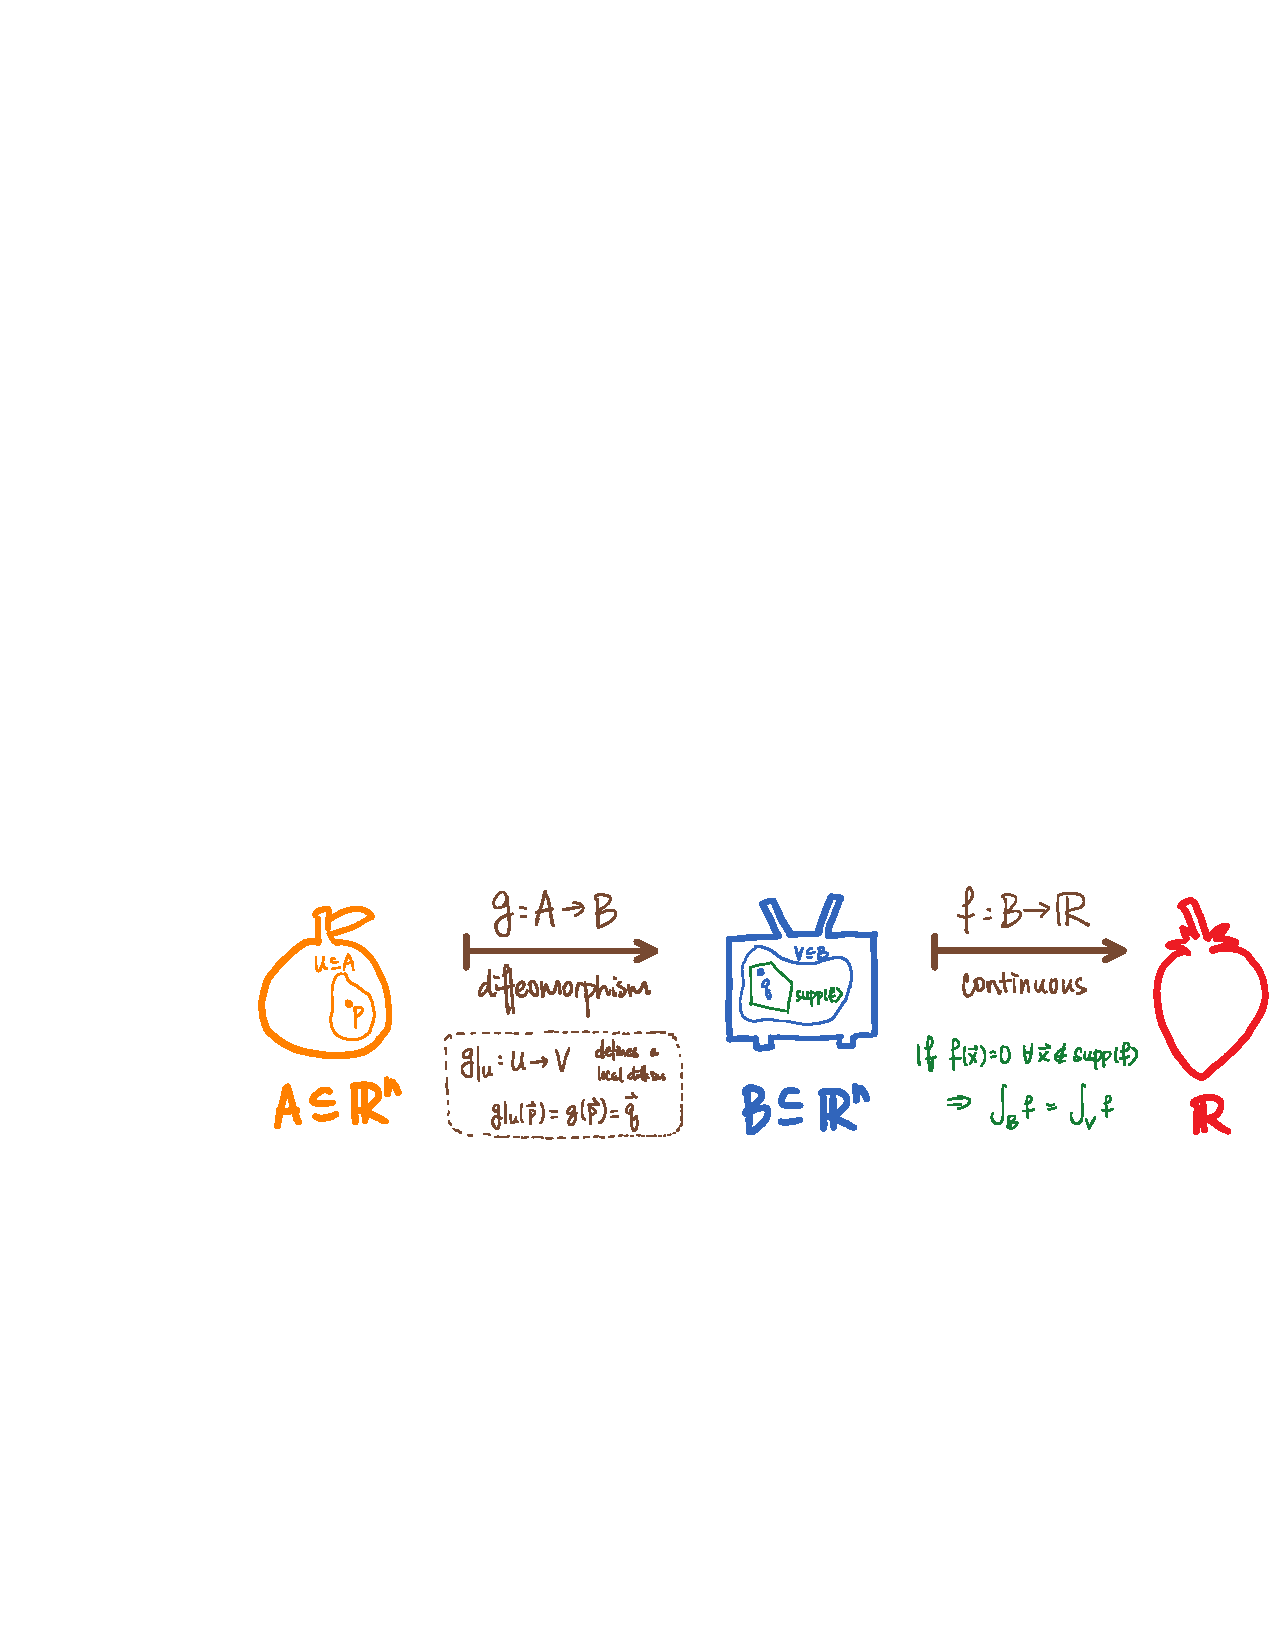
\includegraphics[scale=0.8]{cor13.4.pdf}\\
\text{\color{gray} Figure. Corollary 13.4.1 - Change of Variables and Partition of Unity\color{black}}
\end{center}
\vspace*{\fill}
This text is intended as a Birthday Gift for Chi Han who majors in Mathematical Science in Physics at the University of Michigan. We assume that he has taken one of the course sequences, Math 295-296, or Math 217-297, at the University of Michigan. We will make use of some usual notation that were introduced in those courses. The two course sequences each cover topics related to sets, groups, topology, series and sequences, differentiation and integration of functions of single variable, and linear algebra.\\

In this text, Munkres refers the the text \textit{Analysis on Manifolds}, 1st Edition (1990), by James R. Munkres, published by CRC Press in 2018; Spivak refers to the text \textit{Calculus}, 4th Edition (2008), by Michael Spivak, published by Publish-or-Perish Press in 2008.\\

The class number for 2020 Math 295/296/297 and 2021 Math 395/396 is $57$, but in this text we will use $19$ as our prime number, notice that we have $19\cdot 3 = 57$.\\

This text is edited by Jinyan Miao. The course 2021 Math 395/396 is taught by Professor David Barrett at the University of Michigan - Ann Arbor. Here we give special thanks to Jinyan's friends in 2021 Math 395/396 for helping Jinyan to transcribe notes and correcting typos in this text.\\ 

Except as permitted by both Jinyan and Professor Barrett, no part of this text is allowed to be distributed. This text contains information obtained from authentic sources, but the editors cannot assume responsibility for the validity of all materials in this text or the consequences of their use. The editors have attempted to trace the copyright holders of all material reproduced in this text and apologize to copyright holders if permission to share in this form has not been obtained. If any copyright material has not been acknowledged please write and let us know. If you have any questions or concerns regarding this text, or if you find any typos in this text, please contact Jinyan through jmiu@umich.edu. 


\newpage
\chapter{The Algebra and Topology}

\section[Functions and Sets]{\color{red} Functions and Sets \color{black}}
In the setting of the extended reals, $\R \coloneqq \{-\infty, \infty\}\cup (-\infty, \infty)$, every subset of $\R$ has a supremum and and an infimum. For $S\subseteq \R$, if $\exists\ x \in S$, then we have $\inf S\leq x\leq \sup S$. Notice that we might have $\sup S < \inf S$ in the case where $S = \emptyset$, because we have $\sup \emptyset = -\infty < +\infty = \inf \emptyset$. In this text, occasionally we will use the extended reals setting.\\

\begin{defn}
Let $A$ be an index set, let $X$ be a nonempty set of sets. For $\alpha \in A$, denote $S_\alpha \subseteq X$. $$\bigcup_{\alpha \in A} S_\alpha = \{ x \in X\mid x \in S_\alpha \text{ for at least one } \alpha \in A\}$$
$$\bigcap_{\alpha \in A} S_\alpha = \{x\in X \mid x \in S_\alpha \text{ for all } \alpha \in A\}$$
\end{defn}
In the settings of Definition 1.0.0.0.1, if $A =\emptyset$, we have $\bigcup_{\alpha \in \emptyset}S_\alpha = \emptyset$, and $\bigcap_{\alpha \in \emptyset}S_\alpha = X$.\\


\begin{defn}
Let $A$ be a set, let $S$ be a subset of $A$. The indicator function $\mathbb{I}_S$ is defined by:
$$\mathbb{I}_S: A \to \{0,1\} \qquad a\mapsto \begin{cases} 1 & a \in S \\ 0 & a \notin S\end{cases}$$
\end{defn}

\begin{defn}
Let $A$ be a set, $\Power^{finite}(A)$ denotes the collection of all finite subsets of $A$.\\
Let $A$ be a set, $\Power(A)$ denotes the collection of all subsets of $A$, called the superset of $A$.
\end{defn}

\begin{defn}
Let $A$ be a set. $\# : \Power(A) \to [0,\infty] \ \ \ A' \mapsto \begin{cases}
\text{cardinality of }A' & \text{if }A'  \in \Power^{finite}(A)\\
+ \infty & \text{if }A'  \notin \Power^{finite}(A)
\end{cases}$
\end{defn}


\begin{lem}
Given nonempty $S,T \subseteq \R$ such that $s\leq t$ for all $s \in S$ and $t \in T$.\\
We have the followings:
\begin{enumerate}[topsep=3pt,itemsep=-1ex,partopsep=1ex,parsep=1ex]
\item $\sup(S) = \inf(T) \iff \forall \epsilon>0,\ \exists\ s \in S$ and $t \in T$ such that $t \leq s+\epsilon$.
\item $\sup(S) \leq \inf(T)$
\end{enumerate}
\end{lem}
\newpage


\begin{prop}
Let $S_1,S_2,\cdots, S_k$ be sets, then $\#(S_1\cup S_2\cup \cdots\cup S_k) \leq \#(S_1)+\#(S_2)+\cdots+\#(S_k)$
\end{prop}
\begin{proof}
One might proceed by using induction. Or, we might want to write the following:
$$S_1\cup S_2\cup \cdots \cup S_k = S_1 \cup (S_2\setminus S_1) \cup (S_3\setminus(S_1\cup\S_2))\cup \cdots \cup \left(S_k \setminus\left(\bigcup_{i=1}^{k-1} S_k\right)\right)$$
Hence we have:
\begin{align*}
\#(S_1\cup S_2\cup \cdots \cup S_k) &= \#(S_1) + \#(S_2\setminus S_1) + \#(S_3\setminus(S_1\cup\S_2))+ \cdots + \#\left(S_k \setminus\left(\bigcup_{i=1}^{k-1} S_k\right)\right) \\
&\leq \#(S_1)+\#(S_2)+\cdots+\#(S_k)
\end{align*}
The result follows.
\end{proof}



\newpage
\section[Affine Sets]{\color{red} Affine Sets \color{black}}
\begin{defn}
Let $V$ be a vector space, and let $\vec{p}, \vec{q}, \vec{x} \in V$, where $\vec{p}\neq \vec{q}$. $\vec{p}, \vec{q}, \vec{x}$ are said to be collinear provided that we have $\vec{x}-\vec{p} = t\left(\vec{q}-\vec{p}\right)$ for some scalar $t$. \end{defn}

\begin{defn}
Let $V$ be a vector space over a field $F$, and let $\vec{p}, \vec{q} \in V$, where $\vec{p}\neq \vec{q}$. \\
A line through $\vec{p}, \vec{q}$ is a set $L$ defined by $L \coloneqq \{(1-t)\vec{p}+t\vec{q} \mid t \in F\}$. 
\end{defn}

\begin{defn}Let $V$ be a vector space over a field $F$, let $S$ be a subset of $V$. $S$ is called an affine set provided that $S$ contains all lines through any two vectors in $S$. That is, for $\vec{x},\vec{y} \in S$, and for $t\in F$, $S$ is said to be affine provided that $(1-t)\vec{x} + t\vec{y} \in S$. \end{defn}

\example Let $F$ be a field.\\
$S_1  = \{ (t+1,t,2t),\ t\in F\}$ is a line through $(1,0,0), (2,1,2)$ and $S_1$ is an affine set.\\
$S_2 = \{(x,y,3),\ x,y \in F\}$ is an affine set.\\

\begin{thm}
Let $V$ be a vector space over a field $F$, let $\vec{0}$ be the zero vector in $V$, and let $S\subseteq V$. If we have $\vec{0} \in S$, and $1_F+1_F \neq 0_F$ for $1_F, 0_F \in F$, then $S$ is affine if and only if $S$ is a vector subspace of $V$.
\end{thm}
\begin{proof}
For the $\Leftarrow$ direction, let $\vec{x},\vec{y}\in S$, and let $t$ be a scalar, then $(1-t)\vec{x}+t\vec{y} \in S$ because $S$ is a vector subspace of $V$, hence $S$ is affine. For the $\Rightarrow$ direction, let $\vec{0},\vec{y}\in S$, let $t$ be a scalar, since $S$ is affine, we have $t\vec{y}=t\vec{y}+(1-t)\vec{0}\in S$. Moreover, let $\vec{x},\vec{y} \in S$, since $S$ is affine, then we have $\frac{1}{2}(2\vec{x})+\frac{1}{2}(2\vec{y})\in S$, and here we conclude that $S$ is a vector subspace of $V$.
\end{proof}

\note Let $F = \{0_F,1_F\} = \Z/2\Z$, where we have $1_F+1_F=0_F$. Here, let $V$ be a vector space over the field $F$, let $\vec{p},\vec{q}\in V$, then any line through $\vec{p},\vec{q}$ is the set $\{\vec{p},\vec{q}\}$, hence all two-point sets are lines, and all sets are affine. \\

\remark Not all sets containing $\vec{0}$ will be vector subspaces.

\begin{defn}
Let $V$ be a vector space over a field $F$, let $A,B$ be subsets of $V$, and let $\vec{x}\in V$.
$$V-\vec{x} \coloneqq \{\vec{y}-\vec{x} \mid \vec{y} \in V\} \qquad\qquad\qquad\qquad
A-B \coloneqq \{ \vec{a}-\vec{b}\mid \vec{a} \in A,\vec{b} \in B\}$$
\end{defn}

\begin{lem}
Let $S$ be a subset of a vector space $V$ over a field $F$, and let $\vec{x}\in V$.\\ $S$ is affine if and only if $S-\vec{x}$ is affine.
\end{lem}
\begin{proof}
For the $\Rightarrow$ direction, let $\vec{a},\vec{b}\in S-\vec{x}$, we have $\vec{a} = \vec{m}-\vec{x}$ and $\vec{b} =\vec{n}-\vec{x}$ for some $\vec{m},\vec{n} \in S$. $\forall t \in F$, we have $(1-t)\vec{m}+t\vec{n} \in S$, hence we have $\forall t \in F$, $(1-t)\vec{m}+t\vec{n} -\vec{x}=(1-t)(\vec{m}-\vec{x})+t(\vec{n}-\vec{x}) = \vec{m}-\vec{x}-t\vec{m}+t\vec{x}+t\vec{n}-t\vec{x} = (1-t)\vec{a}+t\vec{b} \in S-\vec{x}$, this shows that $S-\vec{x}$ is affine when $S$ is affine. For the $\Leftarrow$ direction, we assume $S-\vec{x}$ is affine, let $t \in F$, let $\vec{m},\vec{n} \in S$, then $\vec{m}-\vec{x},\vec{n}-\vec{x}\in S-\vec{x}$, hence we know that $(1-t)(\vec{m}-\vec{x})+t(\vec{n}-\vec{x}) \in S-\vec{x}$, which implies $\exists\vec{z}\in S$ such that $\vec{z}-\vec{x} = (1-t)(\vec{m}-\vec{x})+t(\vec{n}-\vec{x}) = \vec{m}-\vec{x}-t\vec{m}+t\vec{x}+t\vec{n}-t\vec{x} = (1-t)\vec{m}+t\vec{n}-\vec{x}$, it follows that $\vec{z} = (1-t)\vec{m}+t\vec{n} \in S$, hence we know that $S$ is also affine. 
\end{proof}

\note Let $S$ be a subset of a vector space $V$ over a field $F$, and let $\vec{x}\in S$, by Theorem 2.1 and Lemma 2.1.1, we can conclude that $S$ is affine if and only if $S-\vec{x}$ is affine if and only if $S-\vec{x}$ is a vector subspace of $V$.

\begin{defn}
Let $S$ be a subset of $V$, where $V$ is a vector space over a field $F$. $\widetilde{S} \coloneqq \{\vec{a}-\vec{b} \mid \vec{a},\vec{b}\in S\}$
\end{defn}

\begin{thm}
Let $V$ be a vector space over a field $F$, let $S$ be a subset of $V$, and let $\vec{x}\in S$.\\ If $S$ is affine, then we have $S - \vec{x} = \widetilde{S}$.
\end{thm}
\begin{proof}
Let $\vec{y}\in S-\vec{x}$, then we have $\vec{y} = \vec{a} - \vec{x}$ for some $\vec{a}, \vec{x}\in S$, which implies $\vec{y} \in \widetilde{S}$, so we have $S-\vec{x} \subseteq \widetilde{S}$. Now let $\vec{k} \in \widetilde{S}$, then we have $\vec{k} = \vec{a}-\vec{b}$ for some $\vec{a},\vec{b}\in S$, which implies $\vec{k} = (\vec{a}-\vec{x})-(\vec{b}-\vec{x})\in S-\vec{x}$.
\end{proof}

\begin{corT}
Let $V$ be a vector space over a field $F$, let $S$ be a subset of $V$.\\ If $S$ is affine, for $\vec{x}_1,\vec{x}_2 \in S$, we have $S-\vec{x}_1 = S-\vec{x}_2$.
\end{corT}

\remark $\widetilde{S}$ is called the vector subspace associated to $S$.\\

\example\\
$\widetilde{S}_1 = \{(t,t,2t)\mid t\in F\}$ is an affine set.\\
$\widetilde{S}_2 = \{(x,y,0)\mid x,y \in F\}$ is an affine set.\\


\remark Let $\vec{a}_1,\vec{a}_2,\cdots, \vec{a}_k$ be a basis of $\widetilde{S}$, where $\widetilde{S}\subseteq V$, and $V$ is a vector space over a field $F$. Write $\widetilde{S} = S - \vec{x}$ for some $\vec{x}\in S$. Then we have the followings: 
$$\widetilde{S} = \{ t_1 \vec{a}_1+t_2\vec{a}_2+\cdots+t_k\vec{a}_k\mid t_j \in F\} \text{ and } S = \{ \vec{x} + t_1 \vec{a}_1+t_2\vec{a}_2+\cdots+t_k\vec{a}_k\mid t_j \in F\}$$

\begin{defn}
Let $S$ be a subset of $V$, where $V$ is a vector space over a field $F$. $S$ is said to be convex provided that $S$ contains all line segments joining two of its points. That is, $S$ is said to be convex provided that $\forall \vec{x},\vec{y}\in S$, and $\forall t \in [0,1]$, we have $(1-t)\vec{x}+t\vec{y}\in S$.
\end{defn}

\example\\
$S_3 = \{ (x,y,3)\mid x^2+y^2\leq 1\}$ is convex but not affine.\\

\begin{defn}
An affine line is an affine set of dimension 1.
\end{defn}

\exercise\\
For $S \subseteq V$, where $V$ is a vector space over $\R$ that has dimension $1$, $S$ is convex if and only if the set $S$ is connected. \\

\exercise\\
Let $V$ be a vector space over $\R$, let $S \subseteq V$, then $S$ is convex if and only if its intersection with each affine line is connected.\\

\newpage
In the rest of this section, when we define a field $F$, we assume that for $1_F,0_F \in F$, $1_F+1_F \neq 0_F$.

\begin{defn}
Let $F$ be a field, let $V,W$ be vector spaces over $F$, and let $T:V\to W$ be a function. Graph$(T) = \{(\vec{v}, \vec{w}) \in V\times W\mid \vec{w} = T\vec{v}\} = \{(\vec{v},T\vec{v})\in V\times W \mid \vec{v}\in V\}$ is called the graph of $T$.
\end{defn}

\begin{defn}
A function $T$ is said to be affine provided that the graph of $T$ is affine.
\end{defn}

\note Let $F$ be a field, let $V,W$ be vector spaces over $F$, and let $T:V\to W$ be a function. If we have $T(\vec{0}) = \vec{0}$, which is equivalent to say $(\vec{0},\vec{0})\in\ $Graph$(T)$, then the followings are equivalent:
\begin{enumerate}[topsep=3pt,itemsep=-1ex,partopsep=1ex,parsep=1ex]
\item $T$ is affine
\item Graph$(T)$ is a vector subspace of $V\times W$
\item For $v_1,v_2 \in V$ and $t \in F$, we have:\\${}$\ \ $(\vec{v}_1+\vec{v}_2, T(\vec{v}_1)+T(\vec{v}_2)) = (\vec{v}_1,T(\vec{v}_1))+(\vec{v}_2,T(\vec{v}_2)) \in Graph(T)$\\${}$\ \ $(t\vec{v}_1,tT(\vec{v}_1)) = t(\vec{v}_1,T(\vec{v}_1)) \in Graph(T)$
\item For $\vec{v}_1,\vec{v}_2\in V, t\in F$, we have:\\${}$\ \  $T(\vec{v}_1+\vec{v}_2) = T(\vec{v}_1)+T(\vec{v}_2)$, and $tT(\vec{v}_1) = T(t\vec{v}_1)$
\item $T$ is linear
\end{enumerate}

\hfill\break
\note Let $F$ be a field, let $V,W$ be vector spaces over $F$, and let $T:V\to W$ be a function, in general we have the followings being equivalent:
\begin{enumerate}[topsep=3pt,itemsep=-1ex,partopsep=1ex,parsep=1ex]
\item $T$ is affine
\item $Graph(T)$ is affine
\item $Graph(T)-(\vec{0},T(\vec{0})) = \{(\vec{v},T(\vec{v})-T(\vec{0}))\mid \vec{v}\in V\}$ is a vector subspace of $V \times W$
\item $L:V\to V\times W \qquad \vec{v}\mapsto T(\vec{v})-T(\vec{0})$ is a linear function
\item $T$ is of the form $T(\vec{v}) = \widetilde{T}(\vec{v})+\vec{b}$ with $\widetilde{T}$ being linear and $\vec{b}\in W$
\end{enumerate}

\exercise From (5), we have $\widetilde{T}$ being uniquely determined, and $\vec{b} = T(\vec{0})$
\newpage

\section[Metric Spaces]{\color{red}Metric Spaces\color{black}}

\begin{defn}
Let $X$ be a set, a function $d:X \times X \to \R$ is said to be a metric on $X$ provided that for $x,y,z\in X$, we have the followings hold:
\begin{enumerate}[topsep=3pt,itemsep=-1ex,partopsep=1ex,parsep=1ex]
\item $d(x,y) = d(y,x)$
\item $d(x,y)\geq 0$, where $d(x,y) = 0$ if and only if $x=y$
\item $d(x,z) \leq d(x,y)+d(y,z)$
\end{enumerate}
\end{defn}

\begin{defn}
A metric space is a set equipped with a metric.
\end{defn}

\begin{defn}
Let $(X,d)$ be a metric space, and let $Y\subseteq X$. The restriction of $d$ on $Y\times Y$, denoted as $d|_{Y\times Y}$, is the induced metric on $Y$, and $(Y,d|_{Y\times Y})$ forms a metric space.
\end{defn}


\example For vector space $\R^n$, the following function is the Euclidean metric on $\R^n$: $$d_{euc}:\R^n\times \R^n\to \R \ \ \ (\vec{x},\vec{y}) \mapsto \sqrt{\sum_{j=1}^n(y_j-x_j)^2}$$

\begin{defn}
Let $(X,d)$ be a metric space, and let $\epsilon>0$. \\
For $x_0\in X$, the set $B_\epsilon(x_0) = \{x \in X\mid d(x_0,x)<\epsilon\}$ is called the $\epsilon$-ball around $x_0$
\end{defn}

\begin{defn}
Let $(X,d)$ be a metric space, let $x_0 \in X$, and let $A \subseteq X$.\\ $x_0$ is interior to $A$ provided that $\exists\ \epsilon>0$ such that $B_\epsilon(x_0) \subseteq A$.\\ $x_0$ is exterior to $A$ provided that $\exists\ \epsilon>0$ such that $B_\epsilon(x_0) \cap A = \emptyset$.\\
$x_0$ is a boundary point of $A$ provided that $\forall \epsilon>0$, $B_\epsilon(x_0)\cap A\neq \emptyset \neq B_\epsilon(x_0)\cap (X\setminus A)$.
\end{defn}
\remark Let $(X,d)$ be a metric space, let $x_0 \in X$. \\
If $x_0$ is neither interior nor exterior to $A\subseteq X$, then $x_0$ is a boundary point of $A$. 

\begin{defn}
Let $A$ be a set. \\
Int$(A) \coloneqq $ The set of interior points of $A$\\
Ext$(A) \coloneqq $ The set of exterior points of $A$\\
Bd$(A) \coloneqq $ The set of boundary points of $A$
\end{defn}

\remark $X =$Int$(A)\ \cup $ Ext$(A)\ \cup $ Bd$(A)$

\begin{defn}
Let $(X,d)$ be a metric space, let $A \subseteq X$, $A$ is said to be open provided that $A =$ Int$(A)$.
\end{defn}
\remark Definition 3.0.0.0.7 defines a topology on $X$.\\

\note Let $(X,d)$ be a metric space, let $A \subseteq X$, and let $x_0 \in X$. The followings hold:
\begin{enumerate}[topsep=3pt,itemsep=-1ex,partopsep=1ex,parsep=1ex]
\item Int$(A)$ is an open subset of $A$, and it contains all open subsets of $A$.
\item $\forall \epsilon>0$, $B_\epsilon(x_0)$ is open.
\item Bd$(X\setminus A) =$Bd$(A)$
\item Bd$(A)$ is closed
\end{enumerate}

\begin{defn}
Let $(X,d)$ be a metric space and let $S\subseteq X$, $S$ is said to be closed provided that $X\setminus S$ is open. 
\end{defn}

\note A set $A$ is closed if and only if $A=$Int$(A)\ \cup$ Bd$(A)$

\begin{defn}
The closure of a set $S$ is the closed superset set of $S$ that is contained in all closed superset of $S$.
\end{defn}

\begin{defn}
Let $(X,d)$ be a metric space, and let $(x_n)$ be a sequence of points in $X$. $(x_n)$ converges to some $x\in X$, denoted as $x_n\to x$, provided that $\forall \epsilon>0$, $\exists\ N \in \N$ such that $d(x_n,x)<\epsilon$ for all $n\in \N$ with $n>N$. $(x_n)$ is said to be convergent provided that $\exists\ x \in X$ such that $x_n \to x$. 
\end{defn}
\note All metric spaces are Hausdorff, the convergence of a sequence in a Hausdorff space is unique. Hence, if $(x_n)$ is a sequence in a metric space $(X,d)$ with $x_n \to x$ and $x_n \to y$, then we have $x=y$.

\begin{defn}
Let $(X,d_x)$ and $(Y,d_y)$ be metric spaces, and let $f:X\to Y$ be a function. $f$ is said to be sequentially continuous at $x\in X$ provided that for all sequence $(x_n)$ in $X$, $x_n \to x$ implies $f(x_n) \to f(x)$.
\end{defn}

\begin{thm}
Let $(X,d_x)$ and $(Y,d_y)$ be metric spaces, and let $f:X\to Y$ be a function. $f$ is sequentially continuous if and only if $f$ is continuous.
\end{thm}

\begin{defn}
Let $(x_n)$ be a sequence of points in a metric space $(X,d)$. $(x_n)$ is said to be Cauchy provided that $\forall \epsilon>0$, $\exists\ N \in \N$ such that $d(x_n,x_m)< \epsilon$ for all $n,m\in\N$ with $n>N$ and $m>N$.
\end{defn}

\begin{defn}
A metric space $(X,d)$ is said to be complete provided that all Cauchy sequences of points in $X$ converge to some $x\in X$.
\end{defn}

\begin{defn}
A set $X$ is said to be sequentially closed provided that all convergent sequence of points in $X$ converges to some $x \in X$.
\end{defn}

\note Here we use $d_{euc}$ to denote the Euclidean metric.
\begin{enumerate}[topsep=3pt,itemsep=-1ex,partopsep=1ex,parsep=1ex]
\item The Euclidean metric space $(\R,d_{euc})$ is complete
\item For $Y \subseteq \R^n$, $(Y,d_{euc})$ is complete if and only if $Y$ is closed
\item $Z \subseteq X$ is closed if and only if $Z$ is sequentially closed 
\end{enumerate}

\begin{defn}
A topological space $(X,\T)$ is said to be compact provided that every open cover of $X$ admits a finite subcover. That is, $(X,\T)$ is said to compact provided that, if we have $X = \bigcup_{\alpha \in A} X_{\alpha}$ where $X_\alpha$ is open in $X$, then $\exists\ \alpha_1,\alpha_2,\cdots,\alpha_k \in A$ such that we have $X =  X_{\alpha_1}\cup X_{\alpha_2}\cup\cdots\cup X_{\alpha_k}$.
\end{defn}

\begin{lem}
$(X,d)$ is compact if and only if every sequence in $X$ admits a convergent subsequence. \end{lem}

\begin{defn}
A metric space $(X,d)$ is said to be sequentially compact provided that every sequence of points in $X$ has a convergent subsequence converging to a point in $X$.
\end{defn}

\begin{lem}
Let $(X,d)$ be a sequentially compact metric space, $\forall \epsilon >0$, we can cover $X$ by finitely many $\epsilon$-ball, in other words, $X$ is totally bounded.
\end{lem}
\begin{proof}
We proceed by contradiction, suppose there exists $\epsilon >0$ that $X$ cannot be covered by finitely many $\epsilon$-balls. let $x_1 \in X$, and let $x_2\notin B_\epsilon (x_1)$. In general, let for $i \in \N$, $x_{i+1}\notin B_\epsilon (x_1)\cup\cdots\cup B_\epsilon (x_i)$, we collect $x_i$ for all $i$ and form a sequence $(x_n)$. It is immediate that $(x_n)$ has no Cauchy subsequence, and hence $(x_n)$ has no convergent subsequence, we reach a contradiction, which completes the proof.
\end{proof}

\begin{thm}[Bolzano-Weierstrass Theorem for metric spaces]
A metric space $(X,d)$ is compact if and only if $(X,d)$ is sequentially compact.
\end{thm}
\begin{proof}
For the $\Rightarrow$ direction, we proceed by contradiction, let $(X,d)$ be a compact metric space, let $(x_n)$ be a sequence of points in $X$ that does not have convergent subsequence. We claim that for all $y \in X$, there exists an open neighborhood $B_y$ for $y$ such that $B_y$ contains only finitely many $x_n$. Here we have $X \subseteq \bigcup_{y \in X} B_y$. Since $X$ is compact, there exists some $k \in \N$ such that $X \subseteq \bigcup_{y_k \in X}^k B_{y_k}$. Note that each $B_{y_k}$ contains finitely many $x_n$, but the finite union of finite sets is finite, and $\{x_n \mid n \in \N\} $ is not finite, here we reach a contradiction, which completes the proof of the $\Rightarrow$ direction. For the $\Leftarrow$ direction, we let $X \subseteq \bigcup_{a \in A} X_a$, where $X_a\subseteq X$ is open, we will show that $X \subseteq X_{a_1}\cup\cdots\cup X_{a_k}$ for some $k \in \N$, and $a_k \in A$. We call $S \subseteq X$ to be Good if $S$ is contained in a finite union of $X_a$, and we call $S\subseteq X$ Bad otherwise. Note that, the finite union of Good sets is Good. We will show that $X$ is Good. We proceed by contradiction, suppose $X$ is bad, then by Lemma 3.1.2, for all $m \in \N$, $\exists\ v_m \in X$ such that $B_\frac{1}{m}(v_m)$ is Bad. We collect the $v_m$, for $m \in \N$, to be a sequence $(v_m)$. By hypothesis, we know that a subsequence $(v_{m_k})$ of $(v_m)$ converges to some $v$ in $X$. Pick $\alpha$ such that $v \in X_\alpha$, then $\exists\ \epsilon>0$ such that $B_\epsilon(v) \subseteq X_\alpha$. Now pick $k$ such that $m_k > \frac{2}{\epsilon}$, and $d(v,v_{m_k}) < \frac{\epsilon}{2}$. Now we can write $B_{\frac{1}{m_k}}(v_{m_k}) \subseteq B_{\epsilon/2}(v_{m_k}) \subseteq B_{\epsilon}(v) \subseteq X_\alpha$ by Triangle inequality, so here we know that $B_{\frac{1}{m_k}}(v_{m_k})$ is Good, a contradiction. This completes the proof.
\end{proof}

\begin{thm}[Bolzano-Weierstrass Theorem for $\R^n$ space]
For $X \subseteq \R^n$ and given Euclidean metric, $X$ is sequentially compact if and only if $X$ is closed and bounded.
\end{thm}
\begin{thm}[Heine-Borel Theorem]
For $X \subseteq \R^n$ with Euclidean metric, $X$ is compact if and only if $X$ is closed and bounded. 
\end{thm}

Notice here, a metric space $(X,d)$ is compact if and only if $(X,d)$ is complete and totally bounded.\\

\exercise Let $(X,d)$ be a metric space, let $\widetilde{d}:X \to \R\ \ \ x\mapsto \min\{ d(x),1\}$.\\ 
Here $\widetilde{d}$ is a metric on $X$. Moreover, $d,\ \widetilde{d}$ induce the same topology on $X$. \\


\newpage
\section[Connectivity and Continuity]{\color{red} Connectivity and Continuity \color{black}}

\begin{defn}
Let $(X,d_X)$ and $(Y,d_Y)$ be metric spaces, let $f:X \to Y$ be a function. $f$ is said to be Lipschitz provided that $\exists\ C \in [0,+\infty)$ such that $d_Y(f(x_1),f(x_2)) \leq C \cdot d_X(x_1,x_2)$ for all $x_1,x_2 \in X$. Here $C$ is called a Lipschitz constant for $f$.
\end{defn}
\note Lipschitz functions are continuous, but continuous functions are not necessarily Lipschitz. For example $f:\R \to \R\ \ \ x\mapsto x^2$ with Euclidean metric, $f$ is continuous but not Lipschitz.\\

\exercise If a function $f$ is Lipschitz, then $\inf(\{x \mid x\text{ is a Lipschitz constant for }f\})$ is also a Lipschitz constant for $f$, that is, the set $\{x \mid x\text{ is a Lipschitz constant for }f\}$ has a minimum value.\\

\begin{defn}
A function $f$ is said to be contraction provided that $f$ is Lipschitz with a Lipschitz constant $C<1$.
\end{defn}

\begin{defn}
A function $f$ is said to be bi-Lipschitz provided that $f$ is a bijection and $f$ and $f^{-1}$ are both Lipschitz. That is, $f$ is said to be bi-Lipschitz provided that $\exists\ C \in [0,+\infty)$ and  $\widetilde{C}\in (0,\infty)$ such that $\widetilde{C}\cdot d_X(x_1,x_2) \leq d_Y(f(x_1),f(x_2)) \leq C d_X(x_1,x_2)$ for all $x_1,x_2 \in X$. 
\end{defn}

\example The function $f:\R \to \R \ \ \ x\mapsto x+\frac{\sin(x)}{19}$ is bi-Lipschitz.

\begin{defn}
For metric spaces $(X, d_X)$ and $(Y, d_Y)$, a function $f:X \to Y$ is called a isometry provided that $d_Y(f(x_1),f(x_2)) = d_X(x_1,x_2)$ for all $x_1,x_2 \in X$. 
\end{defn}

\begin{defn}
Let $h:\R^n \to \R^n$ be a function, $h$ is called an affine isometry provided that $h(\vec{x})= A\vec{x}+\vec{b}$ for some matrix $A$ and vector $\vec{b}\in \R^n$, with $A^TA = I$ where $I$ is the identity matrix. 
\end{defn}

\begin{thm}[Theorem 20.6 on Munkres]
All isometries from $\R^n$ to $\R^n$ are affine isometry.
\end{thm}

\begin{defn}
Let $X$ be a vector space over a field $F$. A function $f: X \times X \to \R$ is a translation-invariant function provided that $f(\vec{x}_1+\vec{y},\vec{x}_2+\vec{y}) = f(\vec{x}_1,\vec{x}_2)$ for all $\vec{x}_1,\vec{x}_2,\vec{y}\in X$.
\end{defn}

\exercise For vector space $X$, if a function $d$ is translation-invariant, then we have $d(\vec{x}_1,\vec{x}_2) = d(\vec{0},\vec{x}_2-\vec{x}_1)$.

\begin{defn}
Let $X$ be a vector space over a field $F$. A function $f:X \times X \to \R$ is a said to be homogeneous provided that $f(t\vec{x}_1,t\vec{x}_2) = |t|\cdot f(\vec{x}_1,\vec{x}_2)$ for all $\vec{x}_1,\vec{x}_2\in X$ and $t \in F$.
\end{defn}


\exercise For vector space $X$, if a function $d$ is homogeneous, then $d(\vec{0},t\vec{x}) = |t|\cdot d(\vec{0},\vec{x})$. \\


\note Let $X$ be a vector space over $\R$, or $\Complex$, let $d$ be a metric on $X$. $d$ is both translation-invariant and homogeneous, and $d(\vec{0},\vec{x})$ is called a norm on $X$.\\


\example For vector space $\R^n$, $||\vec{x}||_p \coloneqq (|x_1|^p + \cdots + |x_n|^p )^\frac{1}{p}$ is a norm when $1\leq p < \infty$.\\
\example For vector space $\R^n$, $|\vec{x}| \coloneqq \max\{|x_1|,\cdots, |x_n|\}$ is a norm on $\R^n$.\\

\note For Euclidean norm $||\vec{x}||$, $|\vec{x}|\leq ||\vec{x}|| \leq  \sqrt{n}|\vec{x}|$.\\ 
Also, we have $||\vec{x}||_p$ tends to $|\vec{x}|$ as $p$ tends to infinity.



\begin{lem}
Let $(X,d)$ and $(Y,d)$ be metric spaces, and let $f:X\to Y$ be a function. Then $f$ is continuous if and only if $f^{-1}(U)$ is open in $X$ when $U$ is open in $Y$, if and only if $f$ is sequentially continuous.
\end{lem}

\begin{prop}
Let $f$ be a Lipschitz function, $f$ is uniformly continuous.
\end{prop}

\begin{prop}
Let $(X,\T)$ be a topological space, the followings are equivalent:
\begin{enumerate}[topsep=3pt,itemsep=-1ex,partopsep=1ex,parsep=1ex]
\item There exists $f:X \to \{0,1\}$ that is a continuous surjective function.
\item There exists nonempty $A \subsetneq X$ that is open and closed in $X$
\end{enumerate}
\end{prop}
\begin{proof}
First we note that, the topology on $\{0,1\}$ is the subspace topology inherited from the Euclidean topology on $\R$, hence we know that $\{1\}$ and $\{0\}$ are both open and closed. To show that (1) implies (2), let $A = f^{-1}(\{1\})$, the result follows. To show that (2) implies (1), we can make use of the indicator function $\mathbb{I}_A: X \to \{0,1\} \ \ \ x\mapsto 1$ if $x \in A$, $0$ if $x \notin A$, then the result follows.
\end{proof}


\begin{prop}
In Euclidean topological space $(\R,\T_{euc})$, the interval $[0,1]$ is connected. 
\end{prop}
\begin{proof}
For any continuous function $f:[0,1]\to \{0,1\}$, $f$ cannot be surjective by the Intermediate Value Theorem. Then the result follows.
\end{proof}

\begin{defn}
Let $(X,\T), (\{0,1\}, \T_E)$ be a topological spaces, where $\T_E$ is the subspace topology on $\{0,1\}$ inherited from the Euclidean topology on $\R$. $X$ is said to be connected provided that for all continuous function $f$ from $X$ to the set $\{0,1\}$, $f$ is not surjective. 
\end{defn}

\begin{defn}
A set $X$ is said to be path connected provided that there exists a continuous function $f:[0,1] \to X$ with $f(0) = \alpha$ and $f(1) = \beta$ for all $\alpha,\beta \in X$.
\end{defn}

\begin{prop}
A path connected topological space is connected.
\end{prop}
\begin{proof}
Let $(X,\T)$ be a path connected topological space. We will show that $X$ is connected, we proceed by contradiction, suppose $X$ is not connected, then there exists $f:X \to \{0,1\}$ that is a continuous surjective function. Pick $\alpha,\beta \in X$ with $f(\alpha) = 0$ and $f(\beta) = 1$. Let $\phi:[0,1] \to X$ be a continuous function with $\phi(0) = \alpha$ and $\phi(1) = \beta$, then we have $f\circ \phi :[0,1] \to \{0,1\}$ being a continuous surjective function, which implies $[0,1]$ is not connected, a contradiction. Hence $X$ must be connected.
\end{proof}
\newpage

\note \begin{enumerate}[topsep=3pt,itemsep=-1ex,partopsep=1ex,parsep=1ex]
\item If $X$ is a convex subset of $\R^n$, then $X$ is path connected.
\item If $X$ is a convex subset of $\R^n$, then $X$ is connected.
\item If $X$ is an open connected subset of $\R^n$, then $X$ is path connected.
\item Let $X=\{(x,y) \in \R^2 \mid x>0,\ y=\sin(\frac{1}{x})\}$, let $Y=\{(0,y)\mid -1\leq y \leq 1\}$,\\ then the set $X\cup Y$ is connected, but not path connected.
\item $GL(n,\R)\coloneqq \{$Invertible $n\times n$ real matrices$\}$ is not connected.
\item $GL_{+}(n,\R)\coloneqq \{ M \in GL(n,\R) \mid \det(M)>0\}$ is path connected.
\item If $X$ is a connected subset of $\R$, then $X$ is an interval or an singleton.
\end{enumerate}
Here (5) can be proved by using the function $f: GL(n,\R) \to \{0,1\} \ \ \ M \mapsto \frac{\frac{\det(M)}{|\det(M)|}+1}{2}$, which is continuous and surjective.\\

\remark The function $p_j : \R^n \to \R \ \ \ (x_1,\cdots,x_j,\cdots, x_n)\mapsto x_j$ is Lipschitz with $C=1$, and hence the function $p_j$ is continuous. \\

\begin{prop}
Let $(X,\T)$ be a topological space. The function $f: X\to \R^n \ \ \ x\mapsto (f_1(x),f_2(x),\cdots, f_n(x))$ is continuous if and only if each function $f_j:X \to \R$ is continuous.
\end{prop}
\begin{proof}
For the $\Rightarrow$ direction, note that $f_j = p_j \circ f$, and the composition of continuous functions is continuous. For the $\Leftarrow$ direction, fix $x_0 \in X$, let $\epsilon>0$, there exists $\delta >0 $ such that $|p_j(x)-f_j(x_0)|< \frac{\epsilon}{\sqrt{n}}$ for $1\leq j \leq n$. For $x \in X$, if we have $d(x,x_0) < \delta$, then we can wrtie $d(f(x),f(x_0)) = ||f(x)-f(x_0)|| \leq \sqrt{n}|f(x)-f(x_0)| < \sqrt{n}\frac{\epsilon}{\sqrt{n}} = \epsilon$, hence $f$ is continuous. This completes the proof.
\end{proof}

\example Consider a function $f$ of the form given by the following: $$f: \R^2 \to \R \ \ \ (x_1,x_2) \mapsto \begin{cases} \frac{x_1x_2}{x_1^2+x_2^2} & (x_1,x_2) \neq (0,0)\\ 0 & (x_1,x_2) = 0 
\end{cases}$$
The function $f$ is continuous when $x_1 \in \R$ is fixed, and continuous when $x_2\in \R$ is fixed, but the function $f$ is not continuous on $\R^2$. This is because the sequence $(a_n)$, where $a_n = (\frac{1}{n},\frac{1}{n})$ converges to $(0,0)$, but $f(\frac{1}{n},\frac{1}{n}) = \frac{1}{2}$ converges to $(\frac{1}{2},\frac{1}{2})$, and $f(0,0) = (0,0)$. 

\chapter{Multivariate Differentiation}
\setcounter{section}{4}
\section[Differentiability]{\color{red} Differentiability \color{black}}
Let $f:\R \to \R$ be a function. $f$ is continuous at $a\in \R$ as a if and only if the graph of $f$ is "almost horizontal" when magnified horizontally at $a$. $f$ is differentiable at $a$ if and only if the graph of $f$ at $a$ is "almost affine," and non-vertical when magnified the same scale in both vertical and horizontal direction. Here we note that the continuity of $f$ at $a$ does not imply its differentiability at $a$.\\

\begin{defn}
Let $V$ be a vector space over a filed $F$. A function $f:V \to V \ \ \ \vec{x}\mapsto \lambda \vec{x}$, for some scalar $\lambda \in F$, is called a dilation centered at $\vec{0}$. A function $d:V \to V \ \ \ \vec{x}\mapsto \lambda \vec{x} + (1-\lambda)\vec{p}$, for $\lambda \in F$ and $\vec{p}\in V$, is called a dilation centered at $\vec{p}$.\\
\end{defn}

In the following discussion, we will try to find a way to define the differentiability of functions in vector spaces. Let $V$ and $W$ be vector spaces over the field $\R$ or the field $\Complex$. Given $f:V \to W$ where Graph$(f) = \{ (\vec{x},f(\vec{x})) \mid \vec{x}\in V\}$. Dilate Graph$(f)$ about the point $(\vec{a},f(\vec{a}))$, we get $(\vec{x},f(\vec{x}))\mapsto (\lambda (\vec{x}-\vec{a})+\vec{a},\lambda (f(\vec{x})-f(\vec{a}))+f(\vec{a}))$. Set $t = \frac{1}{\lambda}$, and set $\vec{u} = \frac{\vec{x}-\vec{a}}{t} \Rightarrow \vec{x} = \vec{a}+t \vec{u}$ for convention. The dilated graph is given by the set: 
$$\left\{(\vec{a}+\vec{u},f(\vec{a})+\frac{f(\vec{a}+t\vec{u})-f(\vec{a})}{t})\mid \vec{u} = \frac{\vec{x}-\vec{a}}{t},\ \vec{x}\in V\right\}$$ 
Consider the case where $t$ tends to $0$. At $\vec{a}\in V$, we are hoping that the following can define an affine function of $\vec{u}$ around the point of interest $\vec{a}$:
$$\vec{u} \mapsto f(\vec{a})+\frac{f(\vec{a}+t\vec{u})-f(\vec{a})}{t}$$ 
To define the the approximation around $\vec{a}$, we hope to find $T(\vec{u})+\vec{b}$ where $\vec{b} = f(\vec{a})$, and $T(\vec{u}) = (f(\vec{a}+t\vec{u})-f(\vec{a}))/t$ being linear. Now the problem reduces to finding a linear function $T$ that satisfies the following:
$$\lim_{t\to 0} \frac{f(\vec{a}+t\vec{u})-f(\vec{a})}{t} = T(\vec{u})$$ If such $T$ exists, then we can write the directional derivative of $f$ at $\vec{a}$ in the direction of $\vec{u}$ as the following:
$$f'(\vec{a};\vec{u}) \coloneqq \lim_{t\to 0} \frac{f(\vec{a}+t\vec{u})-f(\vec{a})}{t}$$ 

\blfootnote{This page number is Jinyan's favorite number}
\newpage

We could try to use this as a core definition for multivariate differential calculus. However, we need to be careful with the following cases:\\

An example in Munkres Section 5 shows that there exists a function $f$ such that all $f'(\vec{0};\vec{u})$ exists but not linear at $\vec{u}$. Also, we might consider the function: $$f(x,y) = \begin{cases} \frac{x^3}{y} & y\neq 0 \\ 0 & y \neq 0\end{cases}$$ here we have $f'(\vec{0};\vec{u}) = 0$ for all $\vec{u}$, and $f(\frac{1}{n},\frac{1}{n^4}) = n$ which does not tends to $0$ when $n$ tends to $\infty$, so $f$ is not sequentially continuous, and hence not continuous at $(0,0)$. Moreover, the Chain Rule for multivariate calculus will fail without stronger assumptions for the differentiability of a function.\\

\note
Let $I$ be an open interval in $\R$, let $W$ be a vector space over a field $F$. Suppose $W$ is equipped with a norm which induces a metric $d$. If $\dim W < \infty$, then all norms on $W$ induce the same topology on $W$, and for metric $d_1$ and $d_2$ for $W$, the identity function $Id:(W,d_1)\to (W,d_2)$ is a bi-Lipschitz function. On another note, for function $f:I \to W$, we write the following: 
$$f'(x)= \lim_{t\to 0} \frac{f(x+t)-f(x)}{t}$$

\example Let $V$ and $W$ be normed vector spaces, let $f:V \to W$ be a function. For $\vec{a},\vec{u} \in V$, we define $g_{\vec{a},\vec{u}}:\R \to V \ \ \ t\mapsto \vec{a}+t\vec{u}$, then $g_{\vec{a},\vec{u}}'(t) = \vec{u}$ for all $t \in \R$. We write: $$(f \circ g_{\vec{a},\vec{u}})'(0)=\lim_{t\to 0}\frac{(f\circ g_{\vec{a},\vec{u}})(t)-(f\circ g_{\vec{a},\vec{u}})(0)}{t} = \lim_{t\to 0} \frac{ f(\vec{a}+t\vec{u})-f(\vec{a})}{t} = f'(\vec{a};\vec{u})$$ Now the directional derivative $f'(\vec{a};\vec{u})$ reduces to derivative of vector-valued function of a scalar. We do not really need $f$ to be defined on all of $V$, we just need $f\circ g_{\vec{a},\vec{u}}$ defined in neighborhood of $0$ in $\R$, in particular, it is good enough to have $\vec{a} \in $Int$($domain of $f)$. \\

\note Let $V$ and $W$ be normed vector spaces over field $\R$ or $\Complex$. For $T \in \hom(V,W)$, the followings are equivalent:
\begin{enumerate}[topsep=3pt,itemsep=-1ex,partopsep=1ex,parsep=1ex]
\item  $\exists\ M \in [0,\infty)$ such that $||T\vec{v}|| \leq M||\vec{v}||\ \forall \vec{v}\in V$, in which we say $T$ is bounded.
\item  $T$ is continuous at $\vec{0}\in V$.
\item  $T$ is Lipschitz.
\item  $T$ is continuous.
\end{enumerate}

\begin{defn}
For normed vector spaces $V$ and $W$: $$B(V,W) \coloneqq \{ T \in \hom(V,W)\mid T \text{ is continuous, bounded, and Lipschitz}\}$$
\end{defn}

\note For normed vector spaces $V$ and $W$, if $dim(V)<\infty$, then $\hom(V,W)= B(V,W)$. That is, the linearity of a function $f \in \hom(V,W)$ implies the continuity of $f$.\\

\newpage
Let $V$ and $W$ be vector spaces over the field $\R$ or the field $\Complex$. Given $f:V \to W$, we dilate Graph$(f)$ about the point $(\vec{a},f(\vec{a}))$, take the limit, the dilated graphs converge point-wise to $\{(\vec{a}+\vec{u},f(\vec{a})+f'(\vec{a};\vec{u})\mid \vec{u}\in V\} = \{(\vec{y}, f(\vec{a})+f'(\vec{a},\vec{y}-\vec{a}))\mid \vec{y}\in V\} =\ $Graph$(\vec{y}\mapsto f(\vec{a})+f'(\vec{a},\vec{y}-\vec{a}))$. To get a good theory, we need the followings hold: 
\begin{enumerate}[topsep=3pt,itemsep=-1ex,partopsep=1ex,parsep=1ex]
\item $f'(\vec{a};\vec{u}) = T(\vec{u})$ is linear in $\vec{u}$.
\item $T$ need to be continuous.
\item We need $f(\vec{a}) + T(\vec{y}-\vec{a}) \approx f(\vec{y})$. That is, let $\vec{h} = \vec{y}-\vec{a}$, we need $f(\vec{a})+T(\vec{h}) \approx f(\vec{a}+\vec{h})$. Here, the error defined by the following should be small compared to $\vec{h}$, or it should tends to $\vec{0}$:  $$\frac{f(\vec{a}+\vec{h}) - f(\vec{a}) - T(\vec{h})}{||\vec{h}||}$$
\end{enumerate}




\begin{defn}
Let $V,W$ be normed vector spaces over the field $\R$ or the field $\Complex$, let $\vec{a}\in A$, where $A$ is an open subset of $V$. For function $f:V \to W$, we write $Df(\vec{a}) = T$ provided that there exists $T \in B(V,W)$ that satisfies the following: $$\lim_{\vec{h}\to \vec{0}} \frac{f(\vec{a}+\vec{h})-f(\vec{a})-T(\vec{h})}{||\vec{h}||} = \vec{0}$$If such $T$ exists, then we write $Df(\vec{a})(\vec{h})=T(\vec{h})$ and $f$ is said to be differentiable at $\vec{a}$.
\end{defn}


\begin{prop}[Munkres Theorem 5.1]
Let $V,W$ be normed vector spaces over the field $\R$ or the field $\Complex$, let $\vec{a}\in A$, where $A$ is an open subset of $V$, and let $f:V \to W$ be a function that is differentiable at $\vec{a}$, for $\vec{u}\in V$, we have $f'(\vec{a};\vec{u}) = Df(\vec{a})(\vec{u})$ where $Df(\vec{a})$ is a linear map from $V$ to $W$.
\end{prop}


\begin{corT}
Let $V,W$ be normed vector spaces over the field $\R$ or the field $\Complex$, let $\vec{a}\in A$, where $A$ is an open subset of $V$, and let $f:V \to W$ be a function that is differentiable at $\vec{a}$. If we have $Df(\vec{a}) = T_1$ and $Df(\vec{a}) = T_2$, then $T_1 = T_2$.
\end{corT}

\exercise Let $V$ and $W$ be vector spaces over the field $\R$ or the field $\Complex$, and consider the function $f:V \to W \ \ \vec{v}\mapsto T(\vec{v})+\vec{b}$ where $T:V\to W$ is a linear transformation and $\vec{b}\in W$. Then the function $f$ is differentiable and $Df(\vec{a}) = T$ for all $\vec{a}\in V$.

\begin{prop}
Let $V,W$ be normed vector spaces over the field $\R$ or the field $\Complex$, let $\vec{a}\in A$, where $A$ is an open subset of $V$, and let $f:V \to W$ be a function that is differentiable at $\vec{a}$. $f$ is continuous at $\vec{a}$.
\end{prop}
\begin{proof}
It suffices to show that $f(\vec{x})$ approaches $f(\vec{a})$ as $\vec{x}$ approaches $\vec{a}$. Here we write $\vec{x} = \vec{a}+\vec{h} \Rightarrow \vec{h} = \vec{x}-\vec{a}$. We need to show that $f(\vec{a}+\vec{h}) - f(\vec{a})$ approaches $\vec{0}$ as $\vec{h}$ approaches $\vec{0}$. Let $T = Df(\vec{a})$.  Notice that we have: 
$$f(\vec{a}+\vec{h}) - f(\vec{a}) = ||\vec{h}||\cdot \frac{f(\vec{a}+\vec{h}) - f(\vec{a})-T(\vec{h})}{||\vec{h}||}+T(\vec{h})\qquad  (*)\coloneqq \frac{f(\vec{a}+\vec{h}) - f(\vec{a})-T(\vec{h})}{||\vec{h}||}$$ Here we have $||f(\vec{a}+\vec{h})-f(\vec{a})|| \leq ||\vec{h}||\cdot ||(*)||+||T(\vec{h})||$. Since $T$ is linear, then $T$ is continuous and hence it is bounded, and tends to $\vec{0}$ as $\vec{h}$ tends to $\vec{0}$. Since $f$ is differentiable, then we know that $(*)$ dents to $\vec{0}$ as $\vec{h}$ tends to $\vec{0}$, hence we conclude that $||\vec{h}||\cdot ||(*)||+||T(\vec{h})||$ tends to $\vec{0}$ as $\vec{h}$ tends to $\vec{0}$. This completes the proof.
\end{proof}
\newpage
\remark Check Munkres Theorem 5.4 for details about the following:\\
Let $V$ be a vector space, and let $f:V \to \R^n$ be a function. For $\vec{v}\in V$, the function $f$ can be written as $f(\vec{v}) = (f_1(\vec{v}),f_2(\vec{v}),\cdots, f_n(\vec{v}))$. We can also write $f$ as the following:
$$f(\vec{v})=\begin{bmatrix}
f_1(\vec{v})\\f_2(\vec{v})\\\vdots\\f_n(\vec{v})
\end{bmatrix}$$
The function $f$ is differentiable at $\vec{a}\in V$ if and only if each $f_j$ is differentiable at $\vec{a}$, and if each $f_j$ is differentiable at $\vec{a}$, then for $\vec{u} \in V$, we can write the following:
$$Df(\vec{a})(\vec{u}) = 
\begin{bmatrix}
Df_1(\vec{a})(\vec{u})\\Df_2(\vec{a})(\vec{u})\\\vdots \\Df_n(\vec{a})(\vec{u})
\end{bmatrix}
$$


\remark \\
Let $W$ be a vector space, let $f:\R^m \to W$ be a function. For $\vec{u} = (u_1,u_2,\cdots,u_m) \in \R^m$, $$Df(\vec{a})\begin{bmatrix}
u_1\\ \vdots \\ u_m
\end{bmatrix} = \sum u_j Df(\vec{a})(\vec{e}_j) = \sum u_j f'(\vec{a};\vec{e}_j) \coloneqq \sum u_j D_jf(\vec{a})
$$ here $D_jf(\vec{a})$ is called a partial derivative of $f$, and we have the following holds: $$Df(\vec{a})(\vec{u}) = [D_1f(\vec{a})\ \cdots\ D_mf(\vec{a})]\ [u_1\ \cdots\ u_m]^T$$
here we note that $[D_1f(\vec{a})\cdots D_mf(\vec{a})]$ is a list of vectors in $W$.\\

\remark \\
For $V = \R^m$, $W = \R^n$, and a differentiable function $f:V \to W$. Each $D_jf(\vec{a})$ is a column vector in $\R^n$. Here we have $[D_1f(\vec{a})\ \cdots D_mf(\vec{a})]$ being an $n\times m$ matrix representing $Df(\vec{a})$. In such matrix, the $(j,k)$ entry is $D_kf_j(\vec{a})$. If we have $n=1$, then $Df(\vec{a}) = [D_1f(\vec{a})\cdots D_mf(\vec{a})]\in \R_{row}^m$ is called the gradient of $f$.\\

\remark \\
Generally, or loosely, if $f$ is differentiable, then $f(\vec{a}+\vec{h}) \approx f(\vec{a}) + Df(\vec{a})(\vec{h})$ for $\vec{h}\approx \vec{0}$, as we result, we can write $f(\vec{x}) \approx f(\vec{a}) + Df(\vec{a}) (\vec{x}-\vec{a})$ for $\vec{x}\approx \vec{a}$.\\

In the following, we will show the Chain Rule holds to multivariate differentiation. Let $V,W,Z$ be normed vector spaces over the field $\R$ or the field $\Complex$, let $f:V \to W$ be a differentiable function. Suppose we have $f(\vec{a})= \vec{b}\in B$ for some $\vec{a}\in V$ and open subset $B$ of $V$, and suppose we have another differentiable function $g:B \to Z$, where $g(f(\vec{x}))\approx g(\vec{b})+Dg(\vec{b})(f(\vec{x})-f(\vec{a}))$ for $f(\vec{x}) \approx f(\vec{a})$, here $f(\vec{x}) \approx f(\vec{a})$ implies $\vec{x}\approx \vec{a}$ suffices. Note that we have the following holds:$$g(f(\vec{x})) \approx g(\vec{b})+Dg(\vec{b})(f(\vec{x})-f(\vec{a})) \approx g(f(\vec{a}))+Dg(\vec{b})(Df(\vec{a})(\vec{x}-\vec{a}))$$ which suggests that $D(g\circ f)(\vec{a}) = Dg(\vec{b})\circ Df(\vec{a})$ here $Dg(\vec{b})$ and $Df(\vec{a})$ are both matrices, hence $\circ$ should be replaced by a $\cdot$ , and this suggests the Chain Rule in multivariate calculus. \\


\begin{thm}[Chain Rule for Multivariate Differentiation]
Let $V,W,Z$ be normed vector spaces over the field $\R$ or the field $\Complex$, let $f:V \to W$ be a differentiable function such that im$(f) = B$ is an open subset of $W$, and let $g:B \to Z$ be a differentiable function. For $\vec{a}\in V$, $D(g\circ f)(\vec{a}) = Dg(\vec{b})\circ Df(\vec{a})$, where $f(\vec{a}) = \vec{b}$.
\end{thm}
\begin{proof}
Write $f(\vec{a}) = \vec{b}\in B$. We want to show that $(**)$ defined by the following approaches $\vec{0}$ as $\vec{h}\in V$ approaches $\vec{0}$: $$(**)\coloneqq\frac{g(f(\vec{a}+\vec{h})) - g(f(\vec{a})) - Dg(\vec{b})(Df(\vec{a})(\vec{h}))}{||h||}$$ Here we define:
$$F(\vec{h}) \coloneqq \begin{cases} \frac{f(\vec{a}+\vec{h})-f(\vec{a})-Df(\vec{a})(\vec{h})}{||h||} & \vec{h}\neq \vec{0} \\ \vec{0}& \vec{h}=\vec{0}\end{cases}\qquad \qquad G(\vec{t}) \coloneqq \begin{cases} \frac{g(\vec{b}+\vec{t})-g(\vec{b})-Df(\vec{b})(\vec{t})}{||t||} & \vec{t}\neq \vec{0} \\ \vec{0}& \vec{t}=\vec{0}\end{cases}$$
One can show that $F$ is continuous at $\vec{0}$ with $F(\vec{0}) = \vec{0}$. \\
Note that here we have $f(\vec{a}+\vec{h}) - f(\vec{a})=Df(\vec{a})(\vec{h})+||\vec{h}||F(\vec{h})$. \\
Similarly, we can write $g(\vec{b}+\vec{k})-g(\vec{b}) = Dg(\vec{b})(\vec{k})+||\vec{k}||G(\vec{k})$, with $G(\vec{0}) = \vec{0}$ and $G$ is continuous at $\vec{0}$, and here we let $\vec{k}\coloneqq f(\vec{a}+\vec{h})-f(\vec{a})$, then we can write the following:

\begin{align*}
(**) &= \frac{g(\vec{b}+\vec{k})-g(\vec{b})-Dg(\vec{b})(Df(\vec{a})(\vec{h}))}{||\vec{h}||} \\&= \frac{Dg(\vec{b})(\vec{k})+||\vec{k}||G(\vec{k})-Dg(\vec{b})(Df(\vec{a}(\vec{h}))}{||\vec{h}||}\\
&= \frac{Dg(\vec{b})(Df(\vec{a})(\vec{h}))+||\vec{h}||Dg(\vec{b})F(\vec{h})+||k||G(\vec{k})-Dg(\vec{b})(Df(\vec{a})(\vec{h}))}{||\vec{h}||}\\
&= Dg(\vec{b})(F(\vec{h}))+\frac{||\vec{k}||}{||\vec{h}||}G(\vec{k})
\end{align*}
As $\vec{h}$ goes to $\vec{0}$, we have $F(\vec{h})$ tends to $\vec{0}$ by continuity, and hence $Dg(\vec{b})(F(\vec{h}))$ tends to $\vec{0}$. Also, as $\vec{h}$ tends to $\vec{0}$, $\vec{k}$ also tends to $\vec{0}$ by definition of $\vec{k}$, and hence $G(\vec{k})$ tends to $\vec{0}$ by continuity. $$\frac{||\vec{k}||}{||\vec{h}||} = \left|\left|Df(\vec{a})\left(\frac{\vec{h}}{||\vec{h}||}\right)+F\left(\vec{h}\right)\right|\right|\leq M\left|\left|\frac{\vec{h}}{||\vec{h}||}\right|\right| = M$$ for some $M \in [0,\infty)$ as $Df(\vec{a})$ and $F$ being continuous, then we know that $(**)$ tends to $\vec{0}$ as $\vec{h}$ tends to $\vec{0}$, and hence the result follows.
\end{proof}

\note Let $f,g$ be functions over vector spaces, if both $f$ and $g$ have all directional derivatives, it is not necessary that $g\circ f$ has all directional derivatives.\\

\remark Let $W$ be a normed vector space, let $\alpha:W\times W \to W \ \ \ (\vec{w}_1,\vec{w}_2)\mapsto \vec{w}_1+\vec{w}_2$, then we know that $\alpha$ is linear and continuous. $D\alpha (\vec{w}_1,\vec{w}_2) = \alpha$.\\


\newpage
\remark Let $V,W$ be normed vector spaces, let $A$ be an open subset of $V$, let $f_1:A \to W$ and $f_2:A \to W$ be functions, and let $g:A \to W\times W \ \ \ \vec{a}\mapsto (f_1(\vec{a}),f_2(\vec{a}))$. If $f_1$ and $f_2$ are both differentiable at $\vec{a}$, then we have $Dg(\vec{a}) = (Df_1(\vec{a}),Df_2(\vec{a}))$. Let $\alpha:W\times W \to W \ \ \ (\vec{w}_1,\vec{w}_2)\mapsto \vec{w}_1+\vec{w}_2$, then if $f_1$ and $f_2$ are differentiable at $\vec{a}$, then $\alpha\circ g: A \to W$ is differentiable at $\vec{a}$ by the Chain Rule, and we have $D(\alpha \circ g)(\vec{a})=D\alpha(g(\vec{a}))(Df_1(\vec{a}),Df_2(\vec{a})) = Df_1(\vec{a})+Df_2(\vec{a})$ \\

\exercise Let $\mu:\R^2 \to \R\ \ \ (x_1,x_2)\mapsto x_1x_2$. We have the following holds:
$$D\mu
\begin{bmatrix} x_1\\ x_2 \end{bmatrix} = \left[
D_1\mu\begin{bmatrix}x_1\\ x_2\end{bmatrix} \ \ D_2\mu\begin{bmatrix}x_1\\ x_2\end{bmatrix}\right] = [x_2\ x_1]$$

\example Let $V$ be a normed vector space. Let $A$ be an open subset of $V$.\\ Let $f_1:A \to \R$ and $f_2: A \to \R$, both are differentiable at $\vec{a}\in A$. We also define:
$$g:A \to \R^2 \ \ \ \vec{a}\mapsto \begin{bmatrix}
f_1(\vec{a}) \\ f_2(\vec{a})
\end{bmatrix} \qquad\qquad\qquad \mu:\R^2 \to \R\ \ \ (x_1,x_2)\mapsto x_1x_2$$
By Chain Rule, we write the following:
\begin{align*}
D(\mu\circ g)(\vec{a})
&=D\mu \begin{bmatrix}
f_1(\vec{a}) \\ f_2(\vec{a})
\end{bmatrix} \begin{bmatrix}
Df_1(\vec{a})\\ Df_2(\vec{a})
\end{bmatrix} \\
&=[f_2(\vec{a}),f_1(\vec{a})]\begin{bmatrix}
Df_1(\vec{a})\\ Df_2(\vec{a})
\end{bmatrix} \\
&= f_2(\vec{a})Df_1(\vec{a})+f_1(\vec{a})Df_2(\vec{a})
\end{align*}

\example Consider $f_1:A \to $Mat$(n,m,\R)$, $f_2:A \to$Mat$(m,p,\R)$, $f_1f_2:A \to$Mat$(n,p,\R)$\\
$$D(f_1f_2)(\vec{a})(\vec{h}) = Df_1(\vec{a})(\vec{h})\cdot f_2(\vec{a})+f_1(\vec{a})\cdot Df_2(\vec{a})(\vec{h})$$

We can also let $f_1$ and $f_2$ be $\Complex$-valued, and identify $a+ib$ with the matrix
$\begin{bmatrix} a & -b \\ b & a \end{bmatrix}$ to get the expected results. 


























\newpage
\section[Continuously Differentiable Functions]{\color{red}Continuously Differentiable Functions \color{black}}
\begin{defn}
Let $V,W$ be vector spaces, let $A$ be an open subset of $V$, let $f:A \to W$ be a function. $f$ is said to be continuously differentiable on $A$ provided that $Df:A \to B(V,W)$ exists and $Df$ is continuous on $A$. In such case, we say $f$ belongs to $C^1(A,W)$.
\end{defn}
\note In the setting of Definition 6.0.0.0.1, the continuity of $Df$ is not automatic, example is included on Munkres Section 6 Exercise 2.\\

\hfill\break
Let $V$ and $W$ be vector spaces, and let $A$ be an open subset of $V$, let $f$ be a function from $V$ to $W$. Suppose $f$ is a differentiable at each $\vec{a}\in A$. For $\vec{h}\in V$, we have $Df(\vec{a})(\vec{h}) \in W$. Here we can write $Df:A \to B(V,W)$, where $B(V,W)$ is a normed space of linear continuous functions. On another note, if we have $V = \R^m$ and $W = \R^n$, then $B(V,W)$ is the matrix space $\text{Mat}_{n\times m}(\R)$. In such case, $A$ is an open subset of $\R^m$, $f:A \to \R^n \ \in C^1$ if and only if $f$ is differentiable at each $\vec{a}\in A$ and  $Df:A \to \text{Mat}_{n\times n}(\R)$ is continuous. In the following, we will show that $f \in C^1$ if and only if each $D_kf_j=f'_j(\vec{a};\vec{e}_k)$ exists and is continuous on $A$. Here $f_j$ denotes the component function of $f$.

\hfill\break
\begin{thm}
Let $A$ be an open subset of $\R^m$, and let $f:A \to \R^n \ \ \ \vec{a}\mapsto (f_1(\vec{a}),f_2(\vec{a}),\cdots, f_n(\vec{a}))$ be a function. If $D_kf_j$ exists and is continuous, then $f \in C^1(A,\R^n)$.
\end{thm}
\begin{proof}
It suffices to show that $f$ is differentiable at each $\vec{a}\in A$, and it suffices to consider $n=1$ by Theorem 5.4 from Munkres Section 5. For $m=2$, let $\vec{a}=(a_1,a_2)$ and $\vec{h}=(h_1,h_2)$, then we can write $f(a_1+h_1,a_2)-f(a_1,a_2) = D_1f(\vec{p})\cdot h_1$ for some $\vec{p}\in \R^2$ by the Mean Value Theorem (MVT), and $f(a_1+h_1,a_2+h_2) - f(a_1+h_1,a_2) = D_2f(\vec{q})\cdot h_2$ for some $\vec{q}\in \R^2$ by the MVT, which implies $f(\vec{a}+\vec{h})-f(\vec{a}) = D_1f(\vec{p})h_1+D_2f(\vec{q})h_2$. Consider the following:
\begin{align*}
\frac{f(\vec{a}+\vec{h})-f(\vec{a})-(D_1f(\vec{a})h_1+D_2f(\vec{a})h_2)}{||\vec{h}||} \tag{1} \end{align*} 
Since $f(\vec{a}+\vec{h})-f(\vec{a}) = D_1f(\vec{p})h_1+D_2f(\vec{q})h_2$,  we can rewrite equation $(1)$ as:
$$(D_1f(\vec{p})-D_1f(\vec{a}))\frac{h_1}{||\vec{h}||} - (D_2f(\vec{q})-D_2f(\vec{a}))\frac{h_2}{||\vec{h}||}$$
Since $D_1f$ and $D_2f$ are continuous, then we know that, when $\vec{h}$ tends to $\vec{0}$, $D_1f(\vec{p})-D_1f(\vec{a})$ and $D_2f(\vec{q})-D_2f(\vec{a})$ tends to zero, and we have $h_1/||\vec{h}||$ and $h_2/||\vec{h}||$ both bounded above by $1$. This shows that the limit for equation (1) as $\vec{h}$ tends to $\vec{0}$ is $0$, and the result for this reduced case follows.
\begin{center}
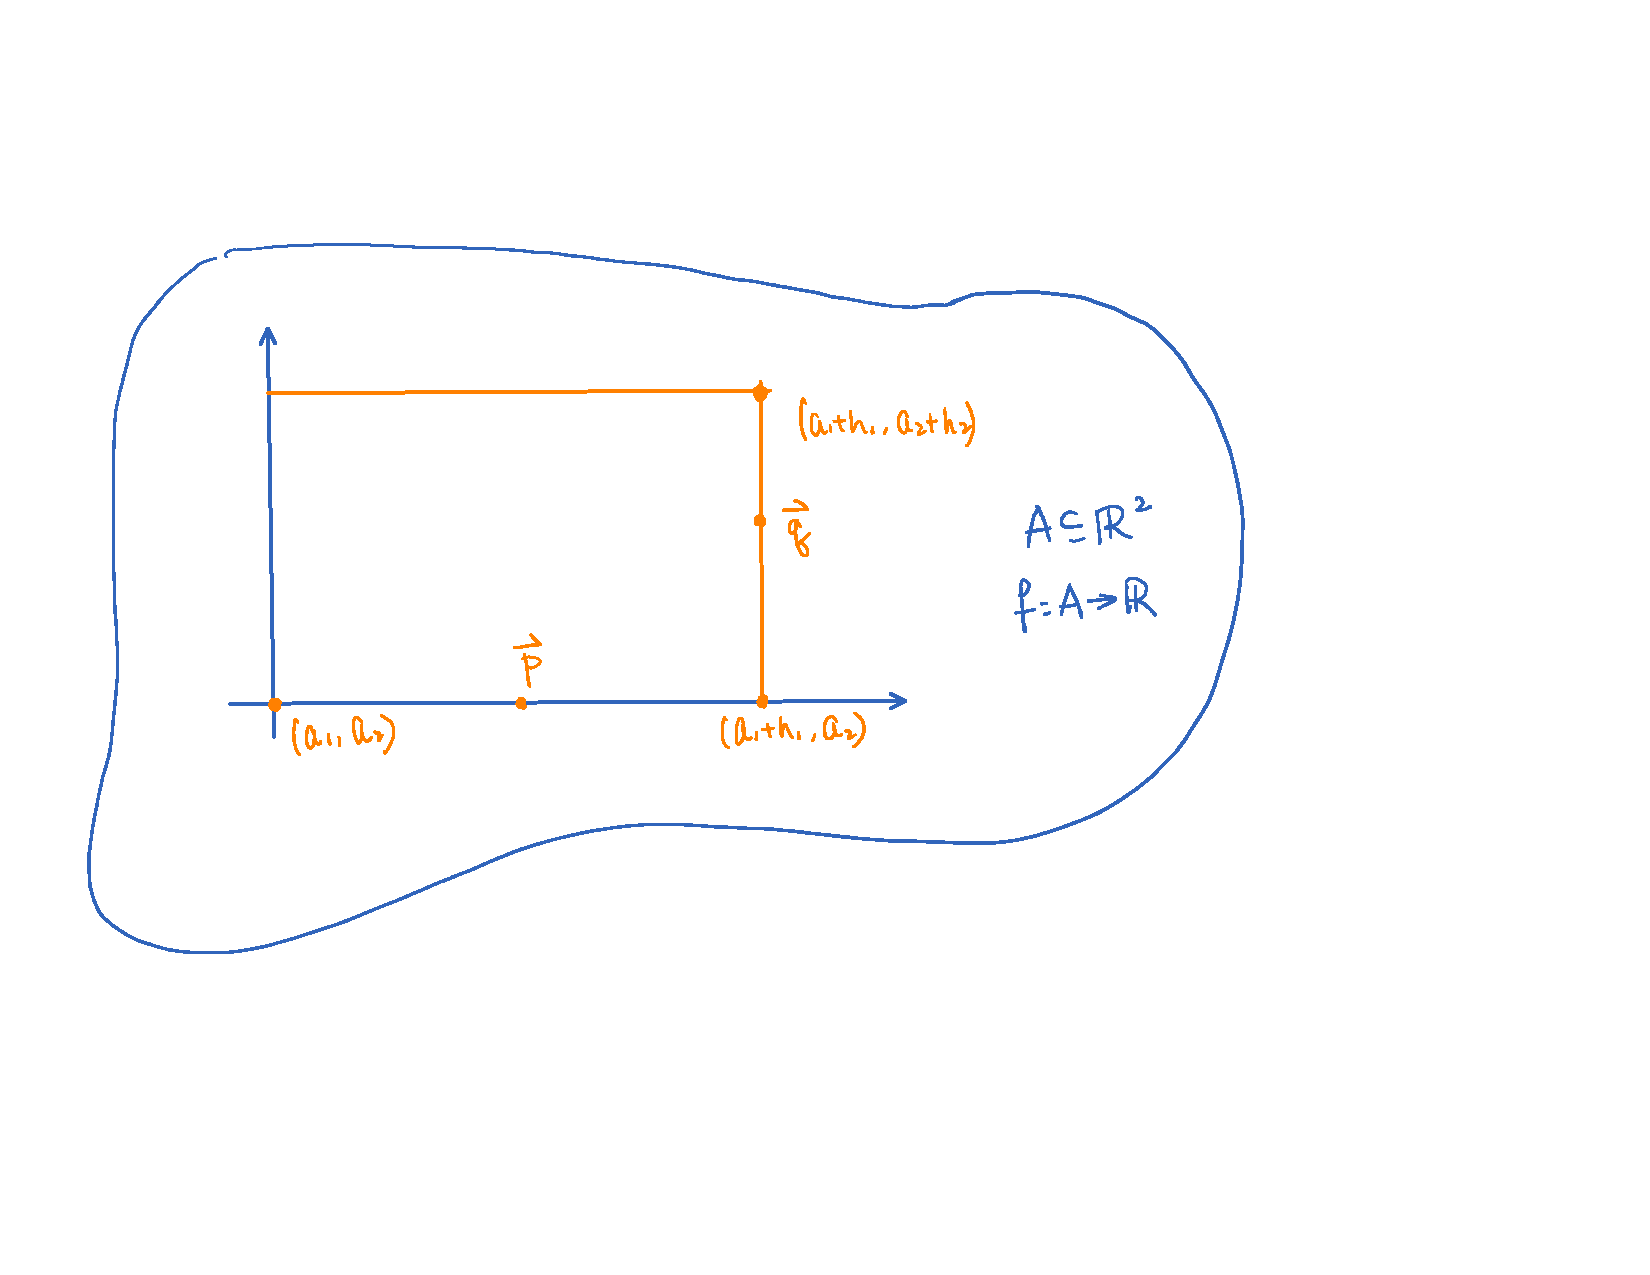
\includegraphics[scale=0.5]{thm6_1.pdf}
\end{center}
The proof for $m>2$ is left for reader, and can be found in Munkres Theorem 6.2.
\end{proof}

Suppose we have a continuous differentiable map from $A$ to $W$, where $A$ is a open subset of a vector space $V$ and $W$ is a vector space. Then we know that $Df:A \to B(V,W)$ is continuous, and $Df$ might be differentiable. If $Df$ is indeed differentiable, then we can define the following:
\begin{defn}
Let $V,W$ be vector spaces, let $A$ be an open subset of $V$, let $f:A \to W$ be a function that belongs to $C^1(A,W)$. We write $f \in C^2(A,W)$ provided that $Df\in C^1(A,B(V,W))$, that is, we write $f \in C^2(A,W)$ provided that $Df$ is differentiable at each $\vec{a}\in A$, and $D^2f$ is continuous on $A$, where $D^2f\coloneqq D(Df): A \to B(V,B(V,W))$
\end{defn}

\remark For vector spaces $V,W$\\ The set $B(V,B(V,W))$ can be viewed as a set of functions from $V \times V$ to $W$.\\

\note For vector spaces $\R^m,\R^n$, let $A$ be an open subset of $\R^m$. If we have that $f:A \to \R^n\ \in C^2(A,\R^n)$, then $f\in C^1(A,\R^n)$ and each $D_{j_1}D_{j_2}f$ exists and is continuous on $A$, Theorem 6.1 provides the converse.

\begin{defn}
Let $V,W$ be vector spaces, let $A$ be an open subset of $V$,\\
$C^0(A,W) = C(A,W)$ is the set of continuous function from $A$ to $W$.
\end{defn}

\begin{defn}
Let $V,W$ be vector spaces, let $A$ be an open subset of $V$,\\
$$C^\infty(A,W) \coloneqq \bigcap_{r \in \N} C^r(A,W)$$
\end{defn}

\note For $r \in \N$, a function $f$ is of $C^r$ type if and only if $Df$  is of $C^{r-1}$ type.

\begin{thm}
Given $f\in C^2(A,\R)$, where $A$ is an open subset of $\R^2$. Then we can write the following: $$D_2D_1f(a,b) = \lim_{(h,k)\to (0,0)} \frac{f(a+h,b+k)-f(a+h,b)-f(a,b+k)+f(a,b)}{hk}$$
\end{thm}
\begin{proof}
Let $\phi:M\to \R \ \ \ s\mapsto f(s,b+k)-f(s,b)$ where $M$ is an open interval contained in $[a,a+h]$. Differentiate $\phi$ using the Chain Rule, we get $\phi'(s) = D_1f(s,b+k) - D_1f(s,b)$. $$\text{Let }num \coloneqq f(a+h,b+k)-f(a+h,b)-f(a,b+k)+f(a,b)$$ Using $\phi'(s) = D_1f(s,b+k) - D_1f(s,b)$, we can write: $$num = \phi(a+h)-\phi(a) = \phi'(s_0)\cdot h = (D_1f(s_0,b+k) - D_1f(s_0,b))\cdot h = D_2D_1f(s_0,t_0)\cdot k \cdot h$$ for some $s_0 \in [a,a+h]$ and $t_0 \in [b, b+k]$ by the Mean Value Theorem. \\
For $\frac{num}{hk} = D_2D_1f(s_0,t_0)$, as $(h,k)$ tends to $(0,0)$, by continuity, we have $D_2D_1f(s_0,t_0)$ tends to $D_2D_1f(a,b)$, the result follows.
\begin{center}
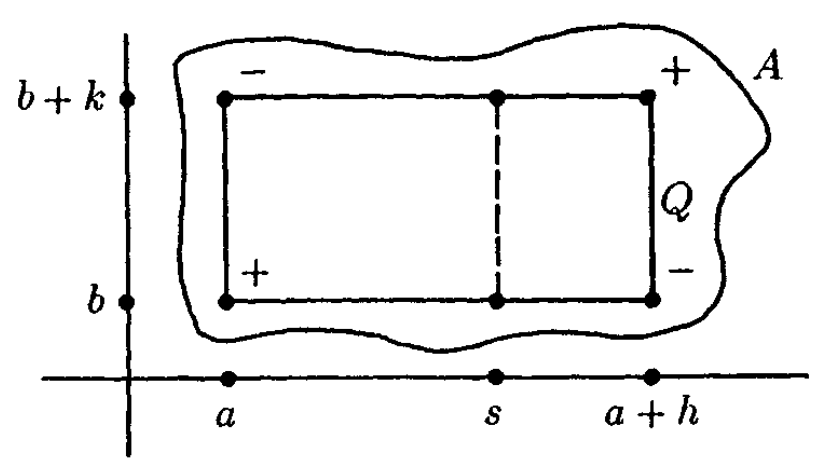
\includegraphics[scale=0.39]{thm6_2.png}${}$\ \ \  \\
(Figure 6.2 from Munkres Section 6)
\end{center}
\end{proof}

\note The existence of $D^2f$ is not enough for this result.\\

\begin{corT}[Clairaut's Theorem]
Given $f\in C^2(A,\R)$, where $A$ is an open subset of normed vector space $V$.\\ We have $D_1D_2f = D_2D_1f$
\end{corT}

\begin{defn}
Let $V,W$ be normed vector spaces, let $A$ be an open subset of $V$, let $f :A \to W$ be a function that is differentiable at $\vec{u}\in A$, we write the following: 
$$D_{\vec{u}} f:A \to W\ \ \ \vec{a}\mapsto f'(\vec{a};\vec{u}) = (Df(\vec{a}))(\vec{u})$$
\end{defn}

\begin{corT}
Given $f\in C^2(A,\R)$, where $A$ is an open subset of normed vector space $V$.\\ We have $D_{\vec{u}_1}D_{\vec{u}_2}f = D_{\vec{u}_2}D_{\vec{u}_1}f$
\end{corT}
\begin{proof}[Proof plan for Corollary 6.2.2]
${}$\\Apply the Chain Rule to $(x_1,x_2) \mapsto f(\vec{a}+x_1\vec{u}_1+x_2\vec{u}_2)$
\end{proof}
\begin{proof}[Another proof plan for Corollary 6.2.2]
${}$\\Adapted from the proof of Theorem 6.2, with the limit: \begin{align*}
lim_{(h,k)\to (0,0)}\frac{f(\vec{a}+h\vec{u}_1+k\vec{u}_2)-f(\vec{a}+h\vec{u}_1)-f(\vec{a}+k\vec{u}_2)+f(\vec{a})}{hk} 
&=D_{\vec{u}_1}D_{\vec{u}_2}f(\vec{a}) \\
&=D_{\vec{u}_2}D_{\vec{u}_1}f(\vec{a})
\end{align*}
The result follows.
\end{proof}

\begin{corT}
Given $f\in C^2(A,\R^m)$, where $A$ is an open subset of normed vector space $V$.\\ We have $D_{\vec{u}_1}D_{\vec{u}_2}f = D_{\vec{u}_2}D_{\vec{u}_1}f$
\end{corT}
\begin{proof}
Apply the proof of Theorem 6.2 to each component function of $f$ and reassemble.
\end{proof}
\remark Theorem 6.2 and its corollaries also work for $f \in C^2(A,W)$ where $W$ is an arbitrary real normed vector space and $A$ is an open subset of $\R^2$. If $\dim W <\infty$, we can use the equivalence of norms to get the result similar to $W = \R^n$. If $\dim W = \infty$, the statements in the theorem and the corollaries are still true, but we need addition tools to prove.\\

Suppose $f\in C^r$, consider $D_{\vec{u}_1}\cdots D_{\vec{u}_r}f$
We can interchange $D\vec{u}_j$ with $D\vec{u}_{j+1}$ by Theorem 6.2 and its corollaries, and hence any arbitrary permutation of $D\vec{u}_i$ can be achieved. \\

\exercise For $f \in C^r(\R^m,\R)$, find the number of distinct $D_{j_1},\cdots D_{j_r} f$.\\

\note For open set $A\subseteq \R^m$ and the function defined by the following: $$f =: A \to \R^n \ \ \ \vec{a}\mapsto  \begin{bmatrix} f_1(\vec{a})\\f_2(\vec{a})\\\vdots\\f_n (\vec{a})\end{bmatrix}$$ 
Here $f\in C^r(A,\R^n)$ if and only if for all $p\leq r$, $D_{j_1} D_{j_2}\cdots D_{j_p}f_r$ exists and is continuous. Also, for each of the $D_{j_1} D_{j_2}\cdots D_{j_p}f_r$, we can interchange the order of $D_{j_t}$ by the discussion above, and rewrite as $D_1^{\alpha_1}D_2^{\alpha_2}\cdots D_m^{\alpha_m}f_r$, where $\alpha_j \in \N\cup \{0\}$, and $|\alpha| = \alpha_1+\alpha_2+\cdots +\alpha_m \leq r$. \\

\note Let $V,W$ be normed vector spaces, and let $A$ be an open subset of $V$, $B$ be an open subset of $W$. Suppose the function $f:A \to B$ is differentiable at $\vec{a}\in A$, and the function $g:B \to A$ is differentiable at $\vec{b} = f(\vec{a}) \in B$, with the property that $g\circ f = Id_A : A \to A \ \ \ \vec{x}\mapsto \vec{x}$. Then by the Chain Rule, we can write $Dg(\vec{b})\cdot Df(\vec{a}) = I$, where $I$ is the identity transformation, which implies $Dg(\vec{b})$ is a left inverse for $Df(\vec{a})$, and we must have $\dim(V) \leq \dim(W)$. Here, if we have $\dim(V) = \dim(W)< \infty$, then  it is immediate that $Dg(\vec{b})$ is a two-sided inverse for $Df(\vec{a})$. Or, if we have $f\circ g = Id_B: B \to B \ \ \ \vec{y}\mapsto \vec{y}$. Then $Dg(\vec{b})$ will also become a two-sided inverse for $Df(\vec{a})$, and we have $\dim(V) = \dim(W)$.\\

\begin{prop}
Let $V,W$ be normed vector spaces with $\dim(V)<\infty$ and $\dim(W) < \infty$, and let $A$ be an open subset of $V$, $B$ be an open subset of $W$. Suppose $f:A \to B$ and $g:B \to A$ are continuous, not necessarily differentiable, with the property $g\circ f = Id_A$ and $f\circ g = Id_B$, then $\dim(V) = \dim(W)$. Here $Id_A$ and $Id_B$ denote the identity transformation in $A$ and in $B$, respectively. \hfill - L. E. J. Brouwer (1912)
\end{prop}

\hfill\break

\exercise There exists a continuous surjection from $\R$ to $\R^2$.\\

\newpage
\section[Homeomorphisms and Diffeomorphisms]{\color{red} Homeomorphisms and Diffeomorphisms \color{black}}

\begin{defn}
A homeomorphism is a continuous bijective function $f$ whose inverse is also continuous. 
\end{defn} 

\example Let $S^1\coloneqq\{(x,y) \in\R^2 \mid x^2 + y^2 = 1\}$.\\
Consider the function $f:[0,2\pi) \to S^1 \ \ \ t\mapsto (\cos(t),\sin(t))$. Notice here $f$ is a bijection, but not a homeomorphism from $[0,2\pi)$ to $S$. This can be shown by considering the sequence $(a_n)$, where $a_i = (\cos(1/i),-\sin(1/i))$. $(a_n)$ converges to $(1,0)$. The sequence $(f^{-1}(a_n))$ converges to $2\pi$, but we have $f^{-1}(-1,0) = 0$, hence $f^{-1}$ is not continuous.

\begin{defn}
Let $A$ be an open subset of normed vector space $V$ and let $B$ be an open subset of normed vector space $W$. A function $f:A \to B$ is called a $C^r$-diffeomorphism provided that $f$ is a bijection, $f\in C^r(A,B)$, and $f^{-1} \in C^r(B,A)$.
\end{defn}

\example $f:\R \to \R \ \ \ t\mapsto t^3$ is a homeomorphism, but not a $C^r$-diffeomorphism. 

\begin{defn}
A complete normed vector space is called a Banach space.
\end{defn}


\example Consider the followings:
$$A = \left\{\begin{bmatrix} r\\\Phi \end{bmatrix} \in \R^2 \mid r>0\right\}\qquad\qquad f:A \to \R^2 \ \ \ \begin{bmatrix} r\\\Phi \end{bmatrix}\mapsto \begin{bmatrix} r\cos(\Phi)\\r\sin(\Phi )\end{bmatrix}$$ 
Here we note that $f$ is of $C^\infty$ type, and we can write the following: $$Df\left(\begin{bmatrix} r\\\Phi \end{bmatrix}\right) = \begin{bmatrix} \cos\left(\Phi\right)& -r\sin\left(\Phi\right)\\\sin\left(\Phi\right)&r\cos\left(\Phi\right) \end{bmatrix}$$
where we have: $$\det\left(Df\left(\begin{bmatrix} r\\\Phi \end{bmatrix}\right)\right) = r$$ here we know that $Df\left(\vec{v}\right)$ is invertible for all $\vec{v} \in A$, but $f$ is not injective on $A$. \\Note that $f\left(A\right) = \R^2 \setminus \{0\}$, and there exists local inverse for $f$ of $C^\infty$ type, but there is no global inverse for $f$.

\begin{defn}
Let $A,B$ be topological spaces, a function $f:A \to B$ is said to be open proved that $f(U)$ is open in $B$ when $U$ is open in $A$.
\end{defn}

\note If a function $f$ is a bijection.
\begin{enumerate}[topsep=3pt,itemsep=-1ex,partopsep=1ex,parsep=1ex]
\item $f$ is continuous if and only if $f^{-1}$ is open.
\item $f$ is open if and only if $f^{-1}$ is continuous.
\item $f$ is a homeomorphism if and only if $f$ is continuous and open.\\
\end{enumerate}
\newpage

\begin{thm}[Inverse Function Theorem]
Let $A $ be an open subset of $\R^n$, let $\vec{a}\in A$, let $f\in C^r(A,\R^n)$ with $r\geq 1$, and given $Df(\vec{a})$ is invertible. There exists an open neighborhood $U$ of $\vec{a}$ such that $f|_U$ is a $C^r$-diffeomorphism, that is, $f$ maps $U$ bijectively to some open set in $\R^n$, and the inverse of $f$ defined by $f^{-1}:f(U) \to U$ is of $C^r$ type. 
\end{thm}
\note $E = \{ \vec{x}\in A\mid Df(\vec{x})$ is invertible $\} = \{\vec{x}\in A \mid \det(Df(\vec{x})) \neq 0\}$ is an open set containing $\vec{a}$. The theorem does not assume that $E=A$, but we could assume such by replacing $A$ by $E$.

\begin{proof}[Proof of the Inverse Function Theorem]
\hfill\break First we need some preliminaries:\begin{enumerate}[topsep=3pt,itemsep=-1ex,partopsep=1ex,parsep=1ex]
\item Let $T_{\vec{a}}$ be a function such that $\vec{x} \mapsto \vec{x}+\vec{a}$
\item Let $g$ denote the function $Df(\vec{a})^{-1}\circ T_{-f(\vec{a})} \circ f\circ T_{\vec{a}}$
\end{enumerate}

From (2), we note that the following holds:
\begin{enumerate}[topsep=3pt,itemsep=-1ex,partopsep=1ex,parsep=1ex]
\item $g(\vec{0}) = \vec{0}$
\item $Dg(\vec{0}) = I$ where $I$ is the identity transformation
\item $f = T_{f(\vec{a})}\circ Df(\vec{a})\circ g\circ T_{-\vec{a}}$
\end{enumerate}

In the following, diffeomorphism refers to $C^r$-diffeomorphism. It suffices to show that $g$ is a diffeomorphism on some open set containing $\vec{0}$. First we let $h = g-Id$, then we know that $Dh = Dg-I$, and $Dh(\vec{0}) = 0$, which implies that each $D_j h_k(\vec{0}) = 0$, $\forall 1\leq j,k \leq n$. Fix $\mu >0$, then there exists $\delta >0$ such that for $\vec{x}\in B_\delta(\vec{0})$, we have each $|D_jh_k(\vec{x})| < \mu$. Let $\vec{x} \in B_\delta(\vec{0})$, consider $Dh(\vec{x})(\vec{u})$. 
$$Dh(\vec{x})(\vec{u}) = \begin{bmatrix}
\sum_j D_jh_1(\vec{x})u_j\\\sum_j D_jh_2(\vec{x})u_j \\ \vdots \\ \sum_j D_j h_n (\vec{x})u_j
\end{bmatrix}$$
\medskip
$$||Dh(\vec{x})(\vec{u})||= \left|\left|\begin{bmatrix}
\sum_j D_jh_1(\vec{x})u_j \\ \vdots \\ \sum_j D_j h_n (\vec{x})u_j
\end{bmatrix}\right|\right|\leq \sqrt{n} \left|\begin{bmatrix}
\sum_j D_jh_1(\vec{x})u_j \\ \vdots \\ \sum_j D_j h_n (\vec{x})u_j
\end{bmatrix}\right| \leq \sqrt{n}n\cdot \mu |\vec{u}|\leq n^\frac{3}{2}\mu ||\vec{u}||$$
which implies the following holds:
$$||Dh(\vec{x})|| \leq n^{\frac{3}{2}} \mu \qquad\qquad\qquad\text{for }\vec{x} \in B_\epsilon(\vec{0})$$
Fix $0 <\epsilon <1$, let $\mu = \epsilon/(n^{3/2})$, then by argument above, there exists $\delta>0$ such that $\forall \vec{x}\in B_\delta(\vec{0})$, we have $||Dh(\vec{x})||<n^{3/2}\mu = \epsilon$. By Lipschitz Estimate from Math 395 HW4, we get $||h(\vec{x}) -h(\vec{y})|| \leq \epsilon ||\vec{x}-\vec{y}||$ for $\vec{x},\vec{y}\in B_\delta(\vec{0})$. Then for $\vec{x},\vec{y}\in B_\delta(\vec{0})$, we have: $$||g(\vec{x})-g(\vec{y})|| = ||\vec{x}-\vec{y} +h(\vec{x})-h(\vec{y})||\leq ||\vec{x}-\vec{y}|| + ||h(\vec{x}) - h(\vec{y})|| \leq (1+\epsilon) ||\vec{x}-\vec{y}||$$
Also, we have the following by the reverse triangle inequality:
$$||g(\vec{x})-g(\vec{y})|| = ||\vec{x}-\vec{y}+h(\vec{x})-h(\vec{y})|| \geq ||\vec{x}-\vec{y}|| - ||h(\vec{x})-h(\vec{y})|| \geq (1-\epsilon)||\vec{x}-\vec{y}||$$
because we have $0< \epsilon<1$, here we see that $g$ is injective on $B_\delta(\vec{0})$.\\ 
Here $B_\delta(\vec{0})$ is a convex set. Let $\psi_y : \vec{x}\mapsto \vec{y}-h(\vec{x})$.\\ 

Pick $0 < \widetilde{\delta} < \delta$ such that for $\vec{y}\in B_{(1-\epsilon)\widetilde{\delta}}(\vec{0})$ and $\vec{x}\in \overline{B_{\widetilde{\delta}}(\vec{0})}$, we have: $$||\psi_y(\vec{x})|| \leq (1-\epsilon)\widetilde{\delta} + \epsilon\widetilde{\delta} = \widetilde{\delta}$$
so the function $\psi_y:\overline{B_{\widetilde{\delta}}(\vec{0})} \to \overline{B_{\widetilde{\delta}}(\vec{0})}$ is well defined, with the following holds:
$$||\psi_y(\vec{x}_1) - \psi_y(\vec{x}_2) || \leq ||h(\vec{x}_2)-h(\vec{x}_1)|| \leq \epsilon||\vec{x}_2-\vec{x}_1||$$
So $\psi_y$ is a contraction on $\overline{B_{\widetilde{\delta}}(\vec{0})}$ where $\overline{B_{\widetilde{\delta}}(\vec{0})}$ is a complete metric space. By the Contraction Mapping Theorem, there exists a unique $\vec{x}\in \overline{B_{\widetilde{\delta}}(\vec{0})}$ such that $\psi_y(\vec{x})= \vec{y}-h(\vec{x}) = \vec{x}$, that is, $g(\vec{x}) = \vec{y}$. Take unions $\bigcup_{\widetilde{\delta} < \delta}\overline{B_{\widetilde{\delta}}(\vec{0})} = B_\delta(\vec{0})$ and $\bigcup_{\widetilde{\delta} < \delta}B_{(1-\epsilon)\widetilde{\delta}}(\vec{0}) = B_{(1-\epsilon)\delta}(\vec{0})$ to get $B_{(1-\epsilon)\delta}(\vec{0}) \subseteq g(B_{\delta}(\vec{0}))\subseteq g(A)$. Notice we get $\vec{0} \in $Int$(g(A))$. \\

We conclude the results that we shown above as a lemma:

\begin{lem}
\setlength{\leftskip}{1cm} Let $A$ be an open subset of $\R^n$, let $\vec{a}\in A$, let $f\in C^r(A,\R^n)$ with $r\geq 1$, and given $Df(\vec{a})$ is invertible. Let $T_{\vec{a}}$ be a function that maps $\vec{x}$ in its domain to $\vec{x}+\vec{a}$ in its codomian, with some $\vec{a}$ in its domain. Let $g$ denote the function $Df(\vec{a})^{-1}\circ T_{-f(\vec{a})} \circ f\circ T_{\vec{a}}$, and let $h = g-Id$ where $Id$ is the identity function. We have the followings hold:
\begin{enumerate}[topsep=3pt,itemsep=-1ex,partopsep=1ex,parsep=1ex,leftmargin=1.5cm]
\item For $\mu>0$, $\exists\ \delta>0$ s.t. $\forall \vec{x}\in B_\delta(\vec{0})$, we have $||Dh(\vec{x})||\leq n^{3/2}\mu$.
\item For $0<\epsilon<1$, $\exists\ \delta>0$ s.t. $\forall \vec{x},\vec{y}\in B_\delta(\vec{0})$, we have $||h(\vec{x})-h(\vec{y})|| \leq \epsilon ||\vec{x}-\vec{y}||$
\item For $0<\epsilon<1$, $\exists\ \delta>0$ s.t. $\forall  \vec{x},\vec{y}\in B_\delta(\vec{0})$, we have the following: $$(1-\epsilon)||\vec{x}-\vec{y}|| \leq ||g(\vec{x})-g(\vec{y})|| \leq (1+\epsilon)||\vec{x}+\vec{y}||$$
\item For $0<\epsilon<1$, $\exists\ \delta>0$ s.t. $g$ is injective on $B_{\delta}(\vec{0})$.
\item For $0<\epsilon<1$, $\exists\ \delta>0$ s.t. $B_{(1-\epsilon)\delta}(\vec{0}) \subseteq g(B_{\delta}(\vec{0}))\subseteq g(A)$.
\item $\vec{0}\in $ Int\,$(g(A))$.
\end{enumerate}
\end{lem}

To proceed proving the Inverse Function Theorem, we will make use of the followings:

\begin{thm}
\setlength{\leftskip}{1cm} Given $E$ as a open subset of $\R^n$, $f \in C^1(E,\R^n)$, and $\det(Df(\vec{x})) \neq 0$ for all $\vec{x}\in E$. Then we have the followings hold:
\begin{enumerate}[topsep=3pt,itemsep=-1ex,partopsep=1ex,parsep=1ex,leftmargin=1.5cm]
\item $\vec{a}\in E$ implies $f(\vec{a}) \in $ Int\,$(f(E))$.
\item $f(E)$ is open in $\R^n$.
\item $f:E \to f(E)$ is an open map.
\end{enumerate}
\end{thm}

\begin{proof}[Proof of Theorem 7.2]
\setlength{\leftskip}{1cm} Fix $\vec{a}\in E$, one can apply Lemma 7.1.1 to the function $g = Df(\vec{a})^{-1} \circ T_{-f(\vec{a})}\circ f \circ T_{\vec{a}}$ defined on the set $T_{-\vec{a}}(E)$. Notice here $g(\vec{0}) = \vec{0}$, and $Dg(\vec{0}) = I$, and we have $\vec{0}\in $Int$($Im$(g))$. Consider $Df(\vec{a})\circ g$, we see that $\vec{0}\in $\,Int$($Im$(Df(\vec{a})\circ g))=$\,Int\,$($Im$(T_{-f(\vec{a})}\circ f\circ T_{\vec{a}}))$. Then we consider $T_{f(\vec{a})}\circ Df(\vec{a})\circ g$, we have $f(\vec{a})\in$Int$($Im$(f\circ T_{\vec{a}}))=$Int$(f(E))$, which implies (1) holds, and (2) follows immediately as $f(E)$ contains all its interior points. For (3), let $U$ be an open subset of $E$, apply (2) to $f|_U$ and the result follows.
\end{proof}

\begin{corT}
\setlength{\leftskip}{1cm} Given $E$ as a open subset of $\R^n$, $f \in C^1(E,\R^n)$, and $\det(Df(\vec{x})) \neq 0$ for all $\vec{x}\in E$. If $f$ is injective, then $f:E \to f(E)$ is a homeomorphism.
\end{corT}


Using Lemma 7.1.1, we know that for $0<\epsilon<1$, $\exists\ \delta>0$ such that $g$ is injective on $B_{\delta}(\vec{0})$. Since $Df(\vec{a})$ is invertible, then $Df(\vec{a})$ is injective. So we know that the composition of injective functions $f|_{B_{\delta}(\vec{a})}=T_{f(\vec{a})} \circ Df(\vec{a}) \circ g|_{B_{\delta}(\vec{0})} \circ T_{-\vec{a}}$ is injective, then by Corollary 7.2.1, let $U = E \cap B_{\delta}(\vec{a})$, where $E$ is the open neighborhood of $\vec{a}$ in which $\det(Df(\vec{t})) \neq 0$ for all $\vec{t}\in E$, then we know that $f|_U: U\to f(U)$ defines a homeomorphism. On the other hand, we know that for all $\vec{x},\vec{y} \in U = B_\delta(\vec{0})$, we have $(1-\epsilon)||\vec{x}-\vec{y}|| \leq ||g(\vec{x}) - g(\vec{y}) || \leq (1+\epsilon) ||\vec{x}+\vec{y}||$, so we know that $g$ is bi-Lipschitz from $B_{\delta}(\vec{0})$ to $g(B_{\delta}(\vec{0}))$. It follows that $f|_U$ is bi-Lipschitz as the composition of bi-Lipschitz functions is bi-Lipschitz. To show that $f|_U$ is a diffeomorphism, we will make use of the following Proposition:


\begin{prop}
\setlength{\leftskip}{1cm} Given $E$ as a open subset of $\R^n$, $f \in C^1(E,\R^n)$ is an injective function, with $\det(Df(\vec{x})) \neq 0$ for all $\vec{x}\in E$. Then we have $f \in C^r$ implies $f^{-1} \in C^r$. 
\end{prop}
\begin{proof}
\setlength{\leftskip}{1cm}It suffices to show that $\psi \coloneqq f^{-1}$ is $C^1$. Fix $\vec{a}\in E$. Let $\vec{b} \in f(\vec{a})$, and let $M\coloneqq Df(\vec{a})$. To show that $\psi$ is differentiable, we want some linear transformation $T$ such that we have the following holds:
\begin{align*}\lim_{\vec{k}\to \vec{0}}\frac{\psi(\vec{b}+\vec{k})-\psi(\vec{b}) - T\vec{k}}{||\vec{k}||} = 0 \tag{1}
\end{align*}
Let $T = M^{-1}$, $\vec{h}= \psi(\vec{b}-\vec{k})-\psi(\vec{b})$, then we can write the following:
\begin{align*}
\frac{\psi(\vec{b}+\vec{k})-\psi(\vec{b}) - M^{-1}\vec{k}}{||\vec{k}||} &= \frac{\vec{h}-M^{-1}\vec{k}}{||\vec{k}||}\\ &= -M^{-1}\left(\frac{\vec{k}-M\vec{h}}{||\vec{k}||}  \right)\\
&= -M^{-1} \left(\frac{f(\vec{a}+\vec{h}) - f(\vec{a}) - M\vec{h}}{||\vec{h}||}  \right)\left(\frac{||\vec{h}||}{||\vec{k}||} \right) \\
&\coloneqq -M^{-1} (*)(**)
\end{align*}
where $(**)$ is bounded for small $||\vec{k}||$ by Lemma 7.1.1 (3), and we have $\vec{h}\to \vec{0}$ as $\vec{k}\to \vec{0}$. While $(*)$ tends to $0$ as $f$ is differentiable, we know that equation (1) must hold. Now we have shown that $\psi$ is differentiable and $D\psi(\vec{b}) = [Df(\psi(\vec{b}))]^{-1}$. Lastly, we will show that $D\psi: f(E) \to $Mat$(n,n,\R)$ is continuous. Here we have:
$$f(E)\xrightarrow[continuous]{\psi}E\xrightarrow[continuous]{Df}GL_{n}(\R) \xrightarrow[continuous]{Inverse}GL_{n}(\R)$$
with $D\psi = \text{(Inverse)} \circ Df \circ \phi$, here $\text{(Inverse)}$ is the function that sends an invertible matrix $M\in GL_{n}(\R)$ to its inverse $M^{-1}\in GL_{n}(\R)$. $\text{(Inverse)}$ is a continuous function by Cramer's Rule and Theorem 2.14 on Munkres. We know that the composition of continuous functions is continuous, hence $D\psi$ is continuous. This finishes the proof for $r=1$. For $r>1$, we can proceed by induction. Assume the result is known for $C^{r-1}$, where $\psi$ and $Df$ are of $C^{r-1}$ type, and we know that $C^{r-1}$ is closed under composition, then the result follows immediately. 
\end{proof}

Here we see that the results for the Inverse Function Theorem follows from Proposition 7.2.2 and Corollary 7.2.1. This completes the proof for the Inverse Function Theorem. \end{proof}

For $V,W,Z$ be normed vector spaces, and let $A$ be a open subset of $V$, $B$ be a subset of $W$. Consider function $f:A \to B$ and $g:B \to Z$, then we can write the chain rule $D(g\circ f) = ((Dg)\circ f) \circ Df$. If we have stronger condition where $f,g \in C^1$, then $Dg,f,Df$ are all continuous, hence we know that the composition of continuous functions $D(g\circ f)\in C^1$. If we have $f \in C^2$, then $D^2f:A \to B(V,B(V,W))$.
Now suppose $f,g \in C^2$, then $Df,Dg\in C^1$, and hence $D(g\circ f) \in C^1$ by the Chain Rule and composition of $C^1$ function, we have $g\circ f \in C^2$. \\ 

\note Consider an affine function $f$ which sends $\vec{x}$ to $T\vec{x}+b$, where $T$ is a linear transformation. We have $Df(\vec{x}) = T$, and $D^2f(\vec{x})=0$, because $T$ is a constant in the space $B(V,W)$.  \\

Let $V$ be a normed vector space, and let $A$ be an open subset of $V$.\\
\exercise Let $f,g \in C^r(A,\R)$, then we have $g\circ f \in C^r$.\\
\exercise Let $f \in C^r(A,\R\setminus\{0\})$, then we have $\frac{1}{f}\in C^r$.\\
\exercise Let $f,g \in C^r(A,\R)$, then we have $f+g \in C^r$, and $fg \in C^r$.\\



\newpage
\textbf{Leibniz's Notation in Several Variables}\\
Suppose we have five quantities, $x,y,u,v,t$, such that any two of these variables determine the other three. Consider the following:
$$f:\begin{bmatrix}
x\\y \end{bmatrix} \mapsto \begin{bmatrix}
u\\v \end{bmatrix}
$$
where we define
$$\begin{bmatrix}
\frac{\partial u}{\partial x} &\frac{\partial u}{\partial y} \\
\frac{\partial v}{\partial x} &\frac{\partial v}{\partial y}
\end{bmatrix} \coloneqq 
Df = \begin{bmatrix}
D_1f_1 & D_2f_2 \\ D_1f_2 & D_2f_2
\end{bmatrix} 
$$
Consider another function defined by the following:
$$g:
\begin{bmatrix}
u\\v
\end{bmatrix}\mapsto t$$
and we define:
$$
\begin{bmatrix}
\frac{\partial t}{\partial u}& \frac{\partial t}{\partial v}
\end{bmatrix} \coloneqq
Dg = \begin{bmatrix}D_1g& D_2g
\end{bmatrix}
$$
Then we write the following:
\begin{align*}
\begin{bmatrix}
\frac{\partial t}{\partial x} & \frac{\partial t}{\partial y}
\end{bmatrix} = D(g\circ f) &= (Dg\circ f)\circ Df 
\\&= \begin{bmatrix}
\frac{\partial t}{\partial u}& \frac{\partial t}{\partial v}
\end{bmatrix} \begin{bmatrix}
\frac{\partial u}{\partial x}&\frac{\partial u}{\partial y}\\
\frac{\partial v}{\partial x}&\frac{\partial v}{\partial y}
\end{bmatrix}
\\&=
\begin{bmatrix}
\frac{\partial t}{\partial u}\frac{\partial u}{\partial x}+\frac{\partial t}{\partial v}\frac{\partial v}{\partial x}& \frac{\partial t}{\partial u}\frac{\partial u}{\partial y} + \frac{\partial t}{\partial v}\frac{\partial v}{\partial y}
\end{bmatrix}
\end{align*}
Notice here, one disadvantage of using the Leibniz's Notation is that the notation "$\frac{\partial t}{\partial u}$" does not specify what quantity is being held fixed when taking the derivative. \\







\newpage
\section[The Implicit Function Theorem]{\color{red}The Implicit Function Theorem \color{black}}
Consider $M \in $Mat$(n,k+n,\R)$, $\vec{c}\in \R^n$, and we define: 
$$E=\{ \vec{v}\in \R^{k+n} \mid M\vec{v} = \vec{c}\}=\{ \vec{v}\in \R^{k+n} \mid M\vec{v}- \vec{c}=\vec{0}\}$$ 
Consider the function $T:\R^{k+n} \to \R^{n} \ \ \ \vec{v}\mapsto M\vec{v}-\vec{c}$, here $T$ is an affine. Let $\hat{M}: \R^{k+n} \to \R^n \ \ \ \vec{v}\mapsto M\vec{v}$. Note here $E$ could be empty, if $E$ is non-empty, then $E $ is an affine set because $E=\ker(\hat{M})+\vec{v}_p$ where $\vec{v}_p$ is any particular solution of $M\vec{v}_p = \vec{c}$. We also have $\dim(E) = \dim(\ker(\hat{M})) = k+n - \text{rank}(M)$ by the Rank-Nullity Theorem. Here we have $k \leq \dim(E) \leq k+n$. \\

In the following discussion, we will investigate if we can write $E$ as Graph$(g)$ for some $g:\R^k \to \R^n$. If such is true, then $g$ has to be affine. Consider the following:
$$M=\begin{bmatrix}
X & Y
\end{bmatrix}\text{ where }X\text{ is an }n\times k\text{ matrix, and } Y \text{ is an }n\times n\text{ matrix}$$
For $\vec{x}\in \R^k$ and $\vec{y}\in \R^n$, we can write the following:
\begin{align*}
M\begin{bmatrix}
\vec{x}\\\vec{y}
\end{bmatrix} = X\vec{x} + Y\vec{y}
\end{align*}

Case (1): $Y$ is non-invertible, then there exists $\vec{w}\in \R^n$ such that $Y\vec{w} = \vec{0}$ with $\vec{w}\neq \vec{0}$.\\ Then for $(\vec{x},\vec{y}) \in E$, we have the following holds:
\begin{align*}
\begin{bmatrix}
\vec{x}\\\vec{y}
\end{bmatrix} \in E \qquad\Rightarrow \qquad \begin{bmatrix}
\vec{x}\\\vec{y}+\vec{w}
\end{bmatrix} \in E
\end{align*}

Case (2): $Y$ is invertible, then we have the following holds:
\begin{align*}
M\begin{bmatrix}
\vec{x}\\\vec{y}
\end{bmatrix} = \vec{c} \iff Y^{-1}X\vec{x} + \vec{y} = Y^{-1}\vec{c} \iff \vec{y} = -Y^{-1}X\vec{x}+ Y^{-1}\vec{c} \coloneqq T(\vec{x})
\end{align*}
Here we see that $T$ is an affine function.\\

Consider $Proj_{k+1,\cdots,n} = [Z\ I]$, where $Z$ is the $n \times k$ zero matrix and $I$ is the $n \times n$ identity matrix. Here we can write the following: $$\hat{Proj_{k+1,\cdots,n}}:\R^{k+n} \to \R^n \ \ \ \begin{bmatrix}\vec{x}\\\vec{y}\end{bmatrix} \mapsto \vec{y}$$
Note here we have $Y = Proj_{k+1,\cdots,n}\cdot M$.\\

Here one might want a different set of $k$ independent vectors on the graph.\\ Let $\hat{p}: \R^{k+n} \to \R^{k+n} \ \ \ \vec{x}\mapsto P\vec{x}$ be a coordinate permutation, where we have: 
$$P = \begin{bmatrix}
 \vec{e}_{j_1} \\ \vec{e}_{j_2} \\ \vdots \\ \vec{e}_{j_{k+n}}
\end{bmatrix}$$
Here we view each standard basis vector $\vec{e}_{j_i}$ as a row vector.\\
The image $\hat{p}($Graph$(g))$ is a coordinate permuted graph with $k$ independent variables. 
\begin{align*}
\dim(&E) = k \iff \text{rank}(M) = n \iff \text{some }n\times n\text{ submatrix of }M\text{ is invertible}\\
&\iff E\text{ is permuted graph of an affine function with k independent variables}
\end{align*}

Consider a general vector in $\R^{k+n}$ defined by the following:
$$\vec{G} = \begin{bmatrix}
\vec{x} \\ \vec{y}
\end{bmatrix}\qquad\qquad\qquad\vec{x}\in \R^k,\ \vec{y}\in \R^n
$$
and a special vector in $\R^{k+n}$ defined by the following:
$$\vec{S} = \begin{bmatrix}
\vec{a} \\ \vec{b}
\end{bmatrix}\qquad\qquad\qquad\vec{a}\in \R^k,\ \vec{b}\in \R^n
$$
The Implicit Function Theorem states that, for $f \in C^r(A,\R^n)$, where $A$ is an open subset of $\R^{k+n}$, and given that the following holds:
\begin{align*}
\begin{bmatrix}
\vec{a}\\\vec{b}
\end{bmatrix} \in f^{-1}(\vec{0}) \coloneqq E \qquad\qquad\qquad \frac{\partial f}{\partial \vec{y}}\begin{bmatrix}
\vec{a}\\\vec{b}
\end{bmatrix} \text{ is invertible}
\end{align*}

Then there exists an open neighborhood $U$ of $\vec{S}$ such that $E \cap U = $Graph$(g)$ for some $g \in C^r(B,\R^n)$ where we have $\vec{a}\in B$ and $B$ is an open subset of $\R^k$. That is, we can solve for $\vec{y}$ in terms of $\vec{x}$ near $\vec{S}$. \\

\begin{thm}[Implicit Function Theorem]
Let $\vec{G}$ in $\R^{k+n}$ defined by the following:
$$\vec{G} = \begin{bmatrix}
\vec{x} \\ \vec{y}
\end{bmatrix}\qquad\qquad\qquad\vec{x}\in \R^k,\ \vec{y}\in \R^n
$$
and fix $\vec{S}$ in $\R^{k+n}$ by the following:
$$\vec{S} = \begin{bmatrix}
\vec{a} \\ \vec{b}
\end{bmatrix}\qquad\qquad\qquad\vec{a}\in \R^k,\ \vec{b}\in \R^n
$$
For $f \in C^r(A,\R^n)$, where $A$ is an open subset of $\R^{k+n}$. If we have the followings hold:
\begin{align*}
\vec{S} \in f^{-1}(\vec{0}) \coloneqq E \qquad\qquad\qquad \left[\frac{\partial f}{\partial \vec{y}}\ \vec{S}\right] \text{ is invertible}
\end{align*}

Then there exists a neighborhood $U$ of $\vec{S}$ such that $E \cap U = $Graph$(g)$ for a unique function $g \in C^r(B,\R^n)$, where $\vec{a}\in B$, and $B$ is an open subset of $\R^k$. In other words, $\exists$ an open neighborhood $B$ of $\vec{x}$ such that $\vec{y} = g(\vec{x})$ and $f(\vec{x},g(\vec{x})) = \vec{0}$ for all $\vec{x}\in B$, with a unique function $g \in C^r(B,\R^n)$.
\end{thm}


\begin{proof}
We will construct a function $F$ to apply the Inverse Function Theorem: $$F:A \to \R^{k+n}\qquad\qquad \begin{bmatrix}
\vec{x}\\\vec{y}
\end{bmatrix} \mapsto \begin{bmatrix}
\vec{x}\\ f\begin{bmatrix}
\vec{x}\\\vec{y}
\end{bmatrix}
\end{bmatrix} \text{\ \ \  for }\vec{x}\in \R^k,\ \vec{y}\in \R^n$$ 

Here we note that $f\begin{bmatrix} \vec{x}\\\vec{y} \end{bmatrix} \in \R^n$, and $F \in C^r(A,\R^{k+n})$ with:
$$DF = \begin{bmatrix}
I & Z \\ 
\frac{\partial f}{\partial \vec{x}}& \frac{\partial f }{\partial \vec{y}}
\end{bmatrix}$$
Here $I$ is the ${k \times k}$ identity matrix, $Z$ is the ${k \times n}$ zero matrix. $\frac{\partial f}{\partial \vec{x}}$ is an ${n \times k}$ matrix, and $\frac{\partial f }{\partial \vec{y}}$ is an ${n \times n}$ matrix. Note that $DF = \det I \cdot \det \frac{\partial f}{\partial \vec{y}} \neq 0$ by Munkres Lemma 2.12. Hence we know that the $DF$ is invertible when evaluated at $\vec{S}$. Here the inverse of $DF$ is given by the following:
$$(DF)^{-1} = \begin{bmatrix}
I & Z \\ -\left(\frac{\partial f}{\partial \vec{x}}\right)^{-1}\frac{\partial f}{\partial \vec{x}} & \left(\frac{\partial f}{\partial \vec{y}}\right)^{-1}
\end{bmatrix}$$
By the Inverse Function Theorem, we know that $F$ has local inverse of $C^{1}$ type, then we can write the following with a function $h$ of $C^r$ type that maps an open set $U\subseteq \R^{k+n}$ to $R^n$, and we get the following:
$$F^{-1}: W \to \R^n \qquad \begin{bmatrix}
\vec{x}\\\vec{z}
\end{bmatrix}  \mapsto \begin{bmatrix}
\vec{x} \\ h\begin{bmatrix}
\vec{x} \\ \vec{z}
\end{bmatrix}
\end{bmatrix} \text{\ \ \  for }\vec{x}\in \R^k,\ \vec{z}\in \R^n$$
Near $\vec{S}$, we have the following holds:
\begin{align*}
\begin{bmatrix}
\vec{x}\\\vec{y}
\end{bmatrix}\in E \iff f\begin{bmatrix}
\vec{x}\\\vec{y}
\end{bmatrix} = \vec{0} \iff F\begin{bmatrix}
\vec{x}\\ \vec{y}
\end{bmatrix}  =\begin{bmatrix}
\vec{x} \\ \vec{0}
\end{bmatrix} &\iff \begin{bmatrix}
\vec{x}\\\vec{y}
\end{bmatrix} = F^{-1}\begin{bmatrix}
\vec{x}\\ \vec{0}
\end{bmatrix}=\begin{bmatrix}
\vec{x} \\ h\begin{bmatrix}
\vec{x} \\ \vec{0}
\end{bmatrix}
\end{bmatrix}  \\&\iff \vec{y} = h\begin{bmatrix}
\vec{x}\\\vec{0}
\end{bmatrix}\coloneqq g(\vec{x})
\end{align*}
One can show that $g$ is unique and the result follows. 
\end{proof}
More details of this proof can be found on Munkres Theorem 9.2.
\hfill\break

In the proof of the Implicit Function Theorem:\\
\remark $F$ gives "change of coordinates" that locally straightens all levels set of $f$. 

\remark $E$ is locally a coordinate permuted graph if rank$(Df(\vec{S}))= n$.


\newpage
\section[Optimization]{\color{red} Optimization \color{black}}

\begin{thm}[First Derivative Test for Higher Dimensions]
Let $\Omega$ be an open subset of $\R^n$, and let $h: \Omega \to \R$ be a function that achieves a local maximum, or minimum, at $\vec{p}\in \Omega$, then $Dh(\vec{p}) = 0$.
\end{thm}
\begin{proof}
Suppose we have $h \in C^1(\Omega, \R)$ where $\Omega$ is an open subset of $\R^n$, with the property that $h$ achieves a maximum, or a minimum, at $\vec{p}\in \Omega$. Consider arbitrary $\gamma \in C^1(A, \Omega)$ with $\gamma(0) = \vec{p}$, where $A$ is an open subset of $\R$. Then $h\circ \gamma$ has a maximum, or a minimum, at $t=0$. So we have $0 = (h \circ \gamma)' (0) = Dh(\gamma(0))\gamma'(0)$. Since this is true for arbitrary $\gamma$ that satisfies $\gamma(0) = \vec{p}$, here we can conclude that $Dh(\gamma(0))=Dh(\vec{p}) = \vec{0}$, and hence we can write: 
$$D_1h(\vec{p}) = D_2h(\vec{p}) = \cdots  = D_nh(\vec{p}) = 0$$

Now assume $h$ has global maximum, or global minimum, at $\vec{p}$. Then for an open subset $U$ that contains $\vec{p}$, $h|_U$ has a local maximum, or a local minimum, and we can reach the same conclusion that $Dh(\vec{p}) = \vec{0}$ with the same argument. That is, $Dh(\vec{p}) = 0$ holds true regardless whether the maximum, or minimum, is global or local.
\end{proof}

\hfill\break
\begin{thm}[Lagrange Multiplier Theorem]
Let $U$ be an open subset of $\R^{k+n}$, let the constraint function be $f\in C^1(U,\R^n)$ with $E=f^{-1}(\vec{0})$, let the objective function be $h\in C^1(U,\R)$, with the property that $h|_E$ has a local maximum , or a local minimum, at $\vec{p}\in E$. Given rank$((Df(\vec{p})) = n$, we have $Dh(\vec{p})$ belongs to the row space of $Df(\vec{p})$, that is, we can write $Dh(\vec{p}) = \lambda_1 Df_1(\vec{p}) + \cdots \lambda_n Df_n(\vec{p})$ for $\lambda_j \in \R$.
\end{thm}

\note The goal of Theorem 9.2 is to maximize, or minimize, the value of the objective function $h$ restricted on the kernel of the constraint function $f$. That is, we want to find $\vec{t}\in \R^{n+k}$ such that $h(\vec{t})$ is maximized, or minimized, whenever $f(\vec{t}) = \vec{0}$ holds. We call such maximum, or minimum, point as $\vec{p}\in \R^{n+k}$. If we have rank$((Df(\vec{p})) = n$, then we can find such $\vec{p}$ with the equation $Dh(\vec{p}) = \lambda_1 Df_1(\vec{p}) + \cdots \lambda_n Df_n(\vec{p})$ for $\lambda_j \in \R$.

\begin{proof}[Proof of Theorem 9.2]
Here we will show the general idea of proving Theorem 9.2, a more general version of this proof is given on Theorem E.2 from Supplement to Munkres. Here we want to maximize, or minimize, $h$ while applying the constraints given by $f$ and its kernel $E$. Consider $\gamma \in C^1(A,E)$, where $A $ is an open subset of $\R$, with $\gamma(0) = \vec{p}$. By Theorem 9.1, we have the following:
\begin{align*}
Dh(\vec{p}) \cdot \gamma' (0) = 0 \tag{1}
\end{align*}

Notice here, we have $f\circ \gamma = \vec{0}$ by construction. Then $Df(\gamma(t)) \cdot \gamma' (t) = 0$, and hence we have the following:
\begin{align*}
\gamma'(0) \in \ker(Df(\vec{p})) \tag{2}
\end{align*}
where $Df(\vec{p}) \in \hom(\R^{k+n},\R^n)$. From Math 395 HW6, we will show that, if $Df(\vec{p})$ has maximal rank $n$, then there are no other constraints applied to $\gamma'(0)$. Then we can combine equation (1) and (2) to get the following: 
\begin{align*}
Dh(\vec{p}) \in (\ker(Df(\vec{p})))^\perp &= ((\text{row space of }Df(\vec{p}))^\perp)^\perp \\&= (\text{row space of }Df(\vec{p})) \\&= \spa\{Df_1(\vec{p}),\cdots, Df_n(\vec{p})\}
\end{align*}
Here we get: 
\begin{align*}
Dh(\vec{p}) = \lambda_1 Df_1(\vec{p})+ \lambda_2 Df_2(\vec{p}) + \cdots \lambda_n Df_n(\vec{p}) \tag{3}
\end{align*}
where $\lambda_i$ are scalars called the Lagrange multipliers.
\end{proof}

\remark From the settings of Theorem 9.2, let $f_i$ denote the component functions of $f$. When maximizing, or minimizing, $h$ with the constraints from $f$, we require $f(\vec{p}) = \vec{0}$, here we will get a set of $n$ equations as we require $f_i(\vec{p}) = 0$ for $1\leq i \leq n$. By equation (3), in order to have to columns of $Dh(\vec{p})$ to match the RHS of the equation (3), we get a set of $n+k$ equations, as we require $D_ih(\vec{p}) = \sum_{j=1}^n D_if_j(\vec{p})$ for $1\leq i \leq n+k$. In total, we will need to solve $k+2n$ unknowns, $k+n$ coordinate components in $\R^{k+n}$ and the $n$ Lagrange multipliers, using the $k+2n$ equations. Here Theorem 9.2 provides us a possible way to solve such optimization problem.\\


\note Suppose $K$ is an compact subset of $\R^n$, let $h: K \to \R$ be a continuous function, then by the Extreme Value Theorem, we know that $h$ has a maximum and a minimum on $K$. By Theorem 9.1, we might want to check the point $\vec{p}\in K$ that satisfies one of the followings to find the local maximum, or local minimum, of $h$:
\begin{enumerate}[topsep=3pt,itemsep=-1ex,partopsep=1ex,parsep=1ex]
\item $\vec{p} \in $Int$(K)$ and $Dh(\vec{p}) = \vec{0}$
\item $\vec{p} \in $Int$(K)$ and $h$ is not differentiable at $\vec{p}$
\item $\vec{p} \in $Bd$(K)$\\
\end{enumerate}

\hfill\break
\example \\
Let the objective function $h(x,y) = x^4+y^6$ be defined on $K=\{(x,y) \mid x^2+y^2 \leq 1\}$. \\We observe that $Dh= [4x^3 \ \ \, 6y^5]$, so $Dh(\vec{x}) = \vec{0}$ only if $\vec{x} = \vec{0}$, and we deduce that $h$ has a minimum at $\vec{0}$, and a maximum somewhere on $Bd(K) \coloneqq E$. Now we want to find such maximum on $E$. Let the constraint function $f(x,y) = x^2+y^2-1$ be defined on $K$, and we have $Df=[2x \ \ \, 2y]$. Notice here, for all $x,y \in \R$ that satisfy $f(x,y) = \vec{0}$, $(x,y) \in \Bd(K)$. Now we get the following equations by Theorem 9.2:
\begin{align*}
\begin{cases}
4x^3 = \lambda 2x & \text{if\ }x=0\Rightarrow y=\pm1 \Rightarrow h=1\\ 
6y^5 = \lambda 2y & \text{if\ }y=0\Rightarrow x=\pm1 \Rightarrow h=1\\ 
x^2+y^2 = 1 & \Rightarrow \lambda/2 + \sqrt{\lambda/3} = 1
\end{cases}
\end{align*}
Here $\lambda$ is the Lagrange multiplier. From such system of equations, we solve that $\lambda = \frac{2}{3}(4-\sqrt{7})$. Check all the critical points, if we have $x = \pm \sqrt{\lambda / 2}$, and $y = \pm\sqrt[4]{\lambda/3}$, we see that $h(x,y) = 0.368$ gives the minimum of $h$ along the boundary $\Bd(K)$. On the other hand, when $x=0, y=\pm1$, or $y=0$, $x=\pm1$, we have $h(x,y) = 1$, hence $max\{$im$(h|_E)\} = 1$. 
\hfill\break

\begin{lem}
Let $X$ be a closed subset of $\R^n$, let $\vec{p}\in \R^n$. Then $f:X \to \R \ \ \ ||\vec{x}-\vec{p}||$ has a minimum. 
\end{lem}
The proof of Lemma 9.2.1 is given on Math 395 HW5 Q5.\\

\example We want to investigate which points in the set $\{(x,y,z) \mid xyz=1\}$ lie closest to $\vec{0}$. Let constraint function be $f(x,y,z) = xyz-1$, and let objective function be $h(x,y,z) = x^2+y^2+z^2$. By Theorem 9.2, we can look for solutions of $f(x,y,z)=0$, with the following holds: 
$$[2x\ \ \, 2y \ \ \, 2z]=Dh = \lambda Df = \lambda[yz\ \ \, xz\ \ \, xy] = [\lambda yz \ \ \, \lambda xz \ \ \, \lambda xy]$$
Here we get the following set of equations:
$$\begin{cases}2x=\lambda yz &\Rightarrow 2x^2 = \lambda\\ 2y=\lambda xz &\Rightarrow 2y^2 = \lambda\\ 2z = \lambda xy &\Rightarrow 2z^2 = \lambda \\ xyz = 1 &\Rightarrow 3\sqrt{\lambda/2}=1  \end{cases}$$
We solve that $\lambda = 2$, and $(x,y,z) = (\pm 1, \pm 1, \pm 1)$ with even numbers of minus sign, so there is a total of four $(x,y,z)$ solutions. All these solutions are the points closest to $\vec{0}$.\\

\example
Let $B\in $ Mat$(n,n,\R)$ be a symmetric matrix, that is, we have $B = B^T$, let $h(\vec{x}) = \vec{x}^T B \vec{x}$. We want to maximize $h$ on the unit sphere $\{\vec{x}\mid ||\vec{x}|| = 1\}$. Let $f(\vec{x}) = ||\vec{x}||^2 - 1$. One might check that $Df(\vec{x})$ has rank $1$ when we have $||\vec{x}||^2 = 1$, and $Df(\vec{x}) = 2\vec{x}^T$. By Theorem 9.2, there exists a solution of this maximization problem when we have $Dh(\vec{x}) = \lambda Df(\vec{x})$. Here we have: 
$$h(\vec{x}) = \sum_{j,k} b_{j,k}x_{j}x_{k} \Rightarrow D_mh(\vec{x}) = \sum_{k} b_{m,k}x_k + \sum_{j} b_{j,m} x_j = 2\sum_{j} b_{j,m}x_j=(2\vec{x}^TB)_m$$ 
It follows that $Dh(\vec{x}) = 2\vec{x}^TB$. \\
Note that one might also write the following to show $Dh(\vec{x}) = 2\vec{x}^TB$:\\
$$Dh(\vec{x}) (\vec{u}) = h'(\vec{x};\vec{u}) = \vec{u}^TB\vec{x}+ \vec{x}^TB\vec{u} = 2\vec{x}^TB\vec{u}$$
Then by Theorem 9.1, we can write the following:
\begin{align*}
Dh(\vec{x}) &= \lambda Df(\vec{x})\\
2\vec{x}^TB &= 2\lambda \vec{x}^T\\
B\vec{x} &= \lambda \vec{x}
\end{align*}
Here we get a system of equations:
\begin{align*}
\begin{cases}B\vec{x} = \lambda\vec{x} \\  ||\vec{x}|| = \vec{x}^T\vec{x}=1  \end{cases} \tag{S1}
\end{align*}

Note here, we are trying to find the eigenvalues and the eigenvectors of unit length for the matrix $B$. Moreover, since the unit sphere $S^{n-1} = \{\vec{x}\mid ||\vec{x}|| = 1\}$ is compact, and we see that $h$ is a continuous function, then we know that $h(S^{n-1})$ is compact and hence $h(S^{n-1})$ admits a maximum value. Combining with Theorem 9.2, we know that there exists at least one solution to the system (S1). That is, there exists at least one eigenvalue $\mu_1$ for $B$ with its eigenvector $\vec{x}_1$, such that $h(\vec{x}_1) = \vec{x}_1^TB\vec{x}_1 = \vec{x}_1^T\mu\vec{x}_1 = \mu\vec{x}_1^T\vec{x}=\mu$ is a maximum of $h$ over the unit sphere $S^{n-1}$. Now we would like to maximize $h$ over $S^{n-1}\cap (\spa\{ \vec{x}_1\})^\perp$, we define $f_{\vec{x}_1}$ by the following:
$$f_{\vec{x}_1}(\vec{x}) =\begin{bmatrix}
 f_1(\vec{x}) \\ f_2(\vec{x})
\end{bmatrix} = \begin{bmatrix}
||\vec{x}||^2 - 1 \\ \vec{x}_1^T\vec{x}
\end{bmatrix} = \begin{bmatrix}
\vec{x}^T\vec{x}-1 \\ \vec{x}_1^T\vec{x}
\end{bmatrix}$$
Notice here we have: $f_{\vec{x}_1}^{-1}(\vec{0}) = S^{n-1}\cap (\spa\{ \vec{x}_1\})^\perp$.
By Theorem 9.2, if such local maximum of $h$ under the constraint from $f$ exists, then the following system of equations must hold:
\begin{align*}
\begin{cases}
\vec{x}^T \cdot \vec{x} = 1\\
\vec{x}_1^T\cdot \vec{x} = 0\\
2\vec{x}^TB = 2\lambda_1 \vec{x}^T + \lambda_2 \vec{x}_1^T 
\end{cases} \tag{S2}
\end{align*}
Here we see that:
$$2\vec{x}^TB = 2\lambda_1 \vec{x}^T + \lambda_2 \vec{x}_1^T \quad \Rightarrow\quad 2\vec{x}^T B \vec{x}_1 = \lambda_2 \quad \Rightarrow\quad 2\mu\vec{x}^T\vec{x}_1 = 0 = \lambda_2$$
So $\lambda_2 = 0$, $\vec{x}^TB = \lambda_1 \vec{x}^T \Rightarrow B\vec{x} = \lambda_1 \vec{x}$. Rewriting system (S2) we get the following:
\begin{align*}
\begin{cases}
\vec{x}^T \cdot \vec{x} = 1\\
\vec{x}_1^T\cdot \vec{x} = 0\\
B\vec{x} = \lambda_1 \vec{x}
\end{cases} \tag{S3}
\end{align*}
Since the orthogonal complement of a subset of a vector space is always closed, then we know that $ S^{n-1}\cap (\spa\{ \vec{x}_1\})^\perp$ is closed and bounded, and hence it is compact, then $h( S^{n-1}\cap (\spa\{ \vec{x}_1\})^\perp)$ is also compact and admits a maximum value. So we know that the system $S3$ has at least one solution for $\lambda_1$ and $\vec{x}$, here we get the second eigenvalue $\mu_2 = \lambda_1$, with eigenvector $\vec{x}_2 \in S^{n-1}\cap (\spa\{ \vec{x}_1\})^\perp$, for the symmetric matrix $B$. One might proceed using induction to show that $B$ admits an orthonormal basis of eigenvectors $\vec{x}_1,\vec{x}_2,\cdots,\vec{x}_n$, with $\mu_1 \geq \mu_2 \geq \cdots \geq \mu_n$. This example proposes a proof for the Spectral Theorem, we conclude our results as the followings:

\begin{lem}
Every symmetric matrix has at least one real eigenvalue. 
\end{lem}

\begin{thm}[Spectral Theorem]
Every symmetric square matrix admits an orthonormal basis of eigenvectors. The corresponding eigenvalues are all real.
\end{thm}

\exercise\\
For a symmetric $n\times n$ matrix $B$, from the previous exercise, $B$ admits a set of maximized real eigenvalues $\{\mu_1,\mu_2,\cdots,\mu_n\}$, with their corresponding eigenvectors $\{\vec{x}_1,\vec{x}_2,\cdots,\vec{x}_n\}$. Let $h(\vec{x}) = \vec{x}^TB\vec{x}$, we have $h(c_1\vec{x}_1 + \cdots + c_n\vec{x}_n) = c_1^2\mu_1 + \cdots + c_n^2 \mu_n$, with the following statements hold:
\begin{enumerate}[topsep=3pt,itemsep=-1ex,partopsep=1ex,parsep=1ex]
\item All $\mu_j \geq 0$ if and only if $\vec{x}^T B \vec{x} \geq 0\ \forall\vec{x} \in \R^n$.
\item All $\mu_j >0$ if and only if $\vec{x}^T B \vec{x} > 0\ \forall\vec{x}\neq \vec{0}\in \R^n$.
\item All $\mu_j \leq 0$ if and only if $\vec{x}^T B \vec{x} \leq 0\ \forall\vec{x} \in \R^n$.
\item All $\mu_j <0$ if and only if $\vec{x}^T B \vec{x} < 0\ \forall\vec{x}\neq \vec{0}\in \R^n$.
\end{enumerate}

\begin{defn}
For a symmetric $n\times n$ matrix $B$, here $B$ admits a set of maximized real eigenvalues $\{\mu_k\mid 1\leq k \leq n\}$, we define the followings:
\begin{enumerate}[topsep=3pt,itemsep=-1ex,partopsep=1ex,parsep=1ex]
\item If $\mu_j \geq 0$ for all $1\leq j \leq n$, then $B$ is said to be positive semi-definite.
\item If $\mu_j > 0$ for all $1\leq j \leq n$, then $B$ is said to be positive definite.
\item If $\mu_j \leq 0$ for all $1\leq j \leq n$, then $B$ is said to be negative semi-definite.
\item If $\mu_j < 0$ for all $1\leq j \leq n$, then $B$ is said to be negative definite.
\end{enumerate}
\end{defn}

\begin{defn}
Let $f$ be a $C^2$ type function defined in a neighborhood of $\vec{x}\in \R^n$. The Hessian $Hf(\vec{x})$ of $f$ at $\vec{x}$ is the $n\times n$ matrix whose entry at $i$-th row, $j$-th column is given by $D_kD_jf(\vec{x})$. 
\end{defn}

\begin{defn}
Symm$(n) \coloneqq \{ M \in $Mat$(n,n) \mid M^T = M \}$
\end{defn}

\begin{thm}[Second Derivative Test for Higher Dimensions]
Let $\Omega$ be an open subset of $\R^n$, let $f \in C^2(\Omega, \R)$, with $Hf(\vec{x})\geq 0$ for all $\vec{x}\in \Omega$. \\
If $Df(\vec{x}_0)= \vec{0}$ for some $\vec{x}_0 \in \Omega$, then $f(\vec{x}) \geq f(\vec{x}_0)$ for all $\vec{x} \in \Omega$. 
\end{thm}
\begin{proof}
We first note that $Hf(\vec{x})\in \Symm(n)$ by Corollary 6.2.1.
Let $\phi(t) = (1-t)\vec{x}_0 + t\vec{x}$. Let $(a_1,a_2,\cdots, a_n) = \vec{a}\coloneqq \phi'(t) = \vec{x}-\vec{x}_0$. We see that we have:
$$(f\circ \phi)'(t) = Df(\phi(t))\vec{a} = \sum_{j} D_jf(\phi(t))a_j$$ Notice here we have $(f\circ \phi)' (0) = 0$, and the following holds:
\begin{align*}
(f\circ \phi)''(t) 
&= \sum_{j} DD_jf(\phi(t)) \cdot \phi'(t)a_j \\
&= \sum_{j,k}D_kD_j f(\phi(t))a_ka_j = \vec{a}^T Hf(\phi(t))\vec{a} \\ &=Hf(\phi(t))\vec{a}^T \vec{a} \geq 0
\end{align*}
We conclude that $f(\vec{x})=(f\circ \phi)(1) \geq (f\circ \phi)(0)=f(\vec{x}_0)$
\end{proof}

\begin{corT}
Let $\Omega$ be an open subset of $\R^n$, let $f \in C^2(\Omega, \R)$, with $Hf(\vec{x})> 0$ for all $\vec{x}\in \Omega$. \\
If $Df(\vec{x}_0)= \vec{0}$ for some $\vec{x}_0 \in \Omega$, then $f(\vec{x}) > f(\vec{x}_0)$ for all $\vec{x} \in \Omega\setminus \{x_0\}$. 
\end{corT}


\begin{defn}
Pos$(n) $ is defined to be the set of positive definite symmetric matrices.
\end{defn}
\note Pos$(n) $ is an open subset of $\Symm(n)$.
\newpage

\begin{thm}[Local Second Derivative Test]
Let $A$ be an open subset of $\R^n$, let $f \in C^2(A , \R)$, let $\vec{x}_0 \in A$ with $Df(\vec{x}_0) = \vec{0}$. \\
Then we have the followings hold:
\begin{enumerate}[topsep=3pt,itemsep=-1ex,partopsep=1ex,parsep=1ex]
\item If we have $Hf(\vec{x}_0) > 0$, then $Hf(\vec{x})>0$ for all $\vec{x}\in B_\delta(\vec{x}_0)$ with some $\delta>0$, and the function $f$ achieves a local minimum at $\vec{x}_0$.
\item If we have $Hf(\vec{x}_0) \ngeq 0$, then $f$ has a strict local maximum at the point $\vec{x}_0$ along some line in $A$, and hence $f$ does not have a local minimum at the point $\vec{x}_0$.
\item If we have  $Hf(\vec{x}_0) < 0$, then $f$ has strict local maximum at $\vec{x}_0$
\item If we have $Hf(\vec{x}_0) \nleq 0$, then $f$ does not have a local maximum at $\vec{x}_0$
\item If we have $Hf(\vec{x}_0)$ is not definite nor semi-definite, then the function $f$ does not have a local max, nor local min, at the point $\vec{x}_0$.
\end{enumerate}
\end{thm}

\begin{corT}
Let $\Omega$ be an open subset of $\R^n$, let $f \in C^2(\Omega, \R)$ with the property that $Hf(\vec{x})\geq 0$ for all $\vec{x}\in \Omega$. Then $f(\vec{x}) \geq f(\vec{x}_0) + Df(\vec{x}_0)(\vec{x}-\vec{x}_0)$ for all $\vec{x}_0,\vec{x}\in \Omega$.
\end{corT}
\begin{proof}
Let $g(\vec{x}) = f(\vec{x}) - Df(\vec{x}_0)(\vec{x}-\vec{x}_0)$, then we have $Dg(\vec{x}) =  Df(\vec{x}) - Df(\vec{x}_0)$, here we note that $Dg(\vec{x}_0) = 0$. Also note that we have $Hg(\vec{x}) = Hf(\vec{x})$. Then by Theorem 9.4, we know that $g(\vec{x}) \geq g(\vec{x}_0) = f(\vec{x}_0)$. The result follows.
\end{proof}

\begin{corT}
Let $\Omega$ be an open subset of $\R^n$, let $f \in C^2(\Omega, \R)$ with the property that $Hf(\vec{x})> 0$ for all $\vec{x}\in \Omega$. Then $f(\vec{x}) > f(\vec{x}_0) + Df(\vec{x}_0)(\vec{x}-\vec{x}_0)$ for all $\vec{x}_0,\vec{x}\in \Omega$ with $\vec{x}_0 \neq \vec{x}$.
\end{corT}


\begin{defn}
Let $\Omega$ be an open subset of $\R^n$, let $\psi : \Omega \to \R$ be a function. \\
The set $\{(\vec{x},y) \in \Omega \times \R \mid y \geq \psi(\vec{x})\}$ is called the epigraph of $\psi$. \\
The set $\{(\vec{x},y) \in \Omega \times \R \mid y \leq \psi(\vec{x})\}$ is called the hypergraph of $\psi$.
\end{defn}


\begin{corT}
Let $\Omega$ be an open subset of $\R^n$, let $\psi \in C^2(\Omega, \R)$ with the property that $H\psi(\vec{x})> 0$ for all $\vec{x}\in \Omega$. We can write the following:
$$\text{epigraph}(\psi) = \bigcap_{\vec{x}_0 \in \Omega} \{ (\vec{x},y) \in \Omega \times \R \mid y\geq \psi(\vec{x}_0)+D\psi (\vec{x}_0) (\vec{x}-\vec{x}_0)\}$$
\end{corT}
\begin{proof}
Here we see that $(\vec{x},y) \in \text{epigraph}(\psi) \Rightarrow (\vec{x},y) \in \text{RHS}$ by Corollary 9.5.2. On the other hand, we have $(\vec{x},y) \in \text{RHS} \Rightarrow y \in \psi(\vec{x}) \Rightarrow (\vec{x},y) \in \text{epigraph}(\psi)$
\end{proof}

\begin{corT}
Let $\Omega$ be an open subset of $\R^n$, let $\psi \in C^2(\Omega, \R)$ with the property that $H\psi(\vec{x})> 0$ for all $\vec{x}\in \Omega$. Then the set epigraph$(\psi)$ is convex.
\end{corT}

\begin{defn}
Let $\Omega$ be a convex subset of $\R^n$, and let $f: \Omega \to \R^n$. The function $f$ is said to be convex provided that the set epigraph$(f)$ is a convex set.
\end{defn}

\remark Corollary 9.5.4 provides us a way to determine if a function $f$ is convex.


\begin{lem}
Let $\Omega$ be a convex subset of $\R^n$, let $f : \Omega \to \R$ be a function. \\ The function $f$ is convex if and only if the following holds: 
$$f((1-t)\vec{x}_0 + t\vec{x}_1) \leq (1-t)f(\vec{x}_0) + tf(\vec{x}_1),\quad \forall \vec{x}_1,\vec{x}_0 \in \Omega,\ 0\leq t \leq 1$$
\end{lem}


\newpage
\chapter{Multivariate Integration}
\setcounter{section}{9}
\section[Integrating Over a Box]{\color{red} Integrating Over a Box \color{black}}
\begin{defn}
Let $a_1,a_2,\cdots, a_n \in \R$, and $b_1,b_2,\cdots,b_n \in \R$, with $a_i \leq b_i$ for all $1 \leq i \leq n$, denote $I_i = [a_i, b_i]\subseteq \R$. $Q \coloneqq [a_1,b_1] \times [a_2,b_2] \times \cdots \times [a_n,b_n] \coloneqq I_1\times I_2 \times \cdots \times I_n$ is called a rectangle, or a box, in  $\R^n$, and $V(Q) \coloneqq (b_1-a_1)(b_2-a_2) \cdots (b_n-a_n) \text{ gives the volume of box }Q$.
\end{defn}
\begin{defn}
For $[a,b]\subseteq \R$ with $a<b$, a partition of $[a,b]$ is a finite collection $P$ of points in $[a,b]$ that includes $a,b$. That is, $P \in \Power^{finite} ([a,b])$ with $a,b\in P$. We index the elements of $P$ in increasing order, as $a =t_0 < t_1 < \cdots < t_k = b$. Each $[t_{i-1},t_i]$ for $1\leq i \leq k$ is called a subinterval determined by $P$.
\end{defn}
\begin{defn}
For a box $Q = [a_1,b_1] \times [a_2,b_2] \times \cdots \times [a_n,b_n] \in \R^n$, a partition $P$ of $Q$ is an $n$-tuple $(P_1,P_2,\cdots,P_n)$ such that $P_j$ is a partition of $[a_j,b_j]$ for $1 \leq j \leq n$. Let $I_j$ be one of the subintervals determined by $P_j$ of the interval $[a_j,b_j]$, the box $R\coloneqq I_1 \times I_2 \times \cdots \times I_n$ is called a subbox, or subrectangle, determined by $P$, of the box $Q$. 
\end{defn}

Let $Q$ be a box in $\R^n$, and let $P$ be a partition of $Q$. Consider a bounded function $f:Q \to \R$. In the following figure, we assume $n=2$ for simplicity. 
\begin{center}
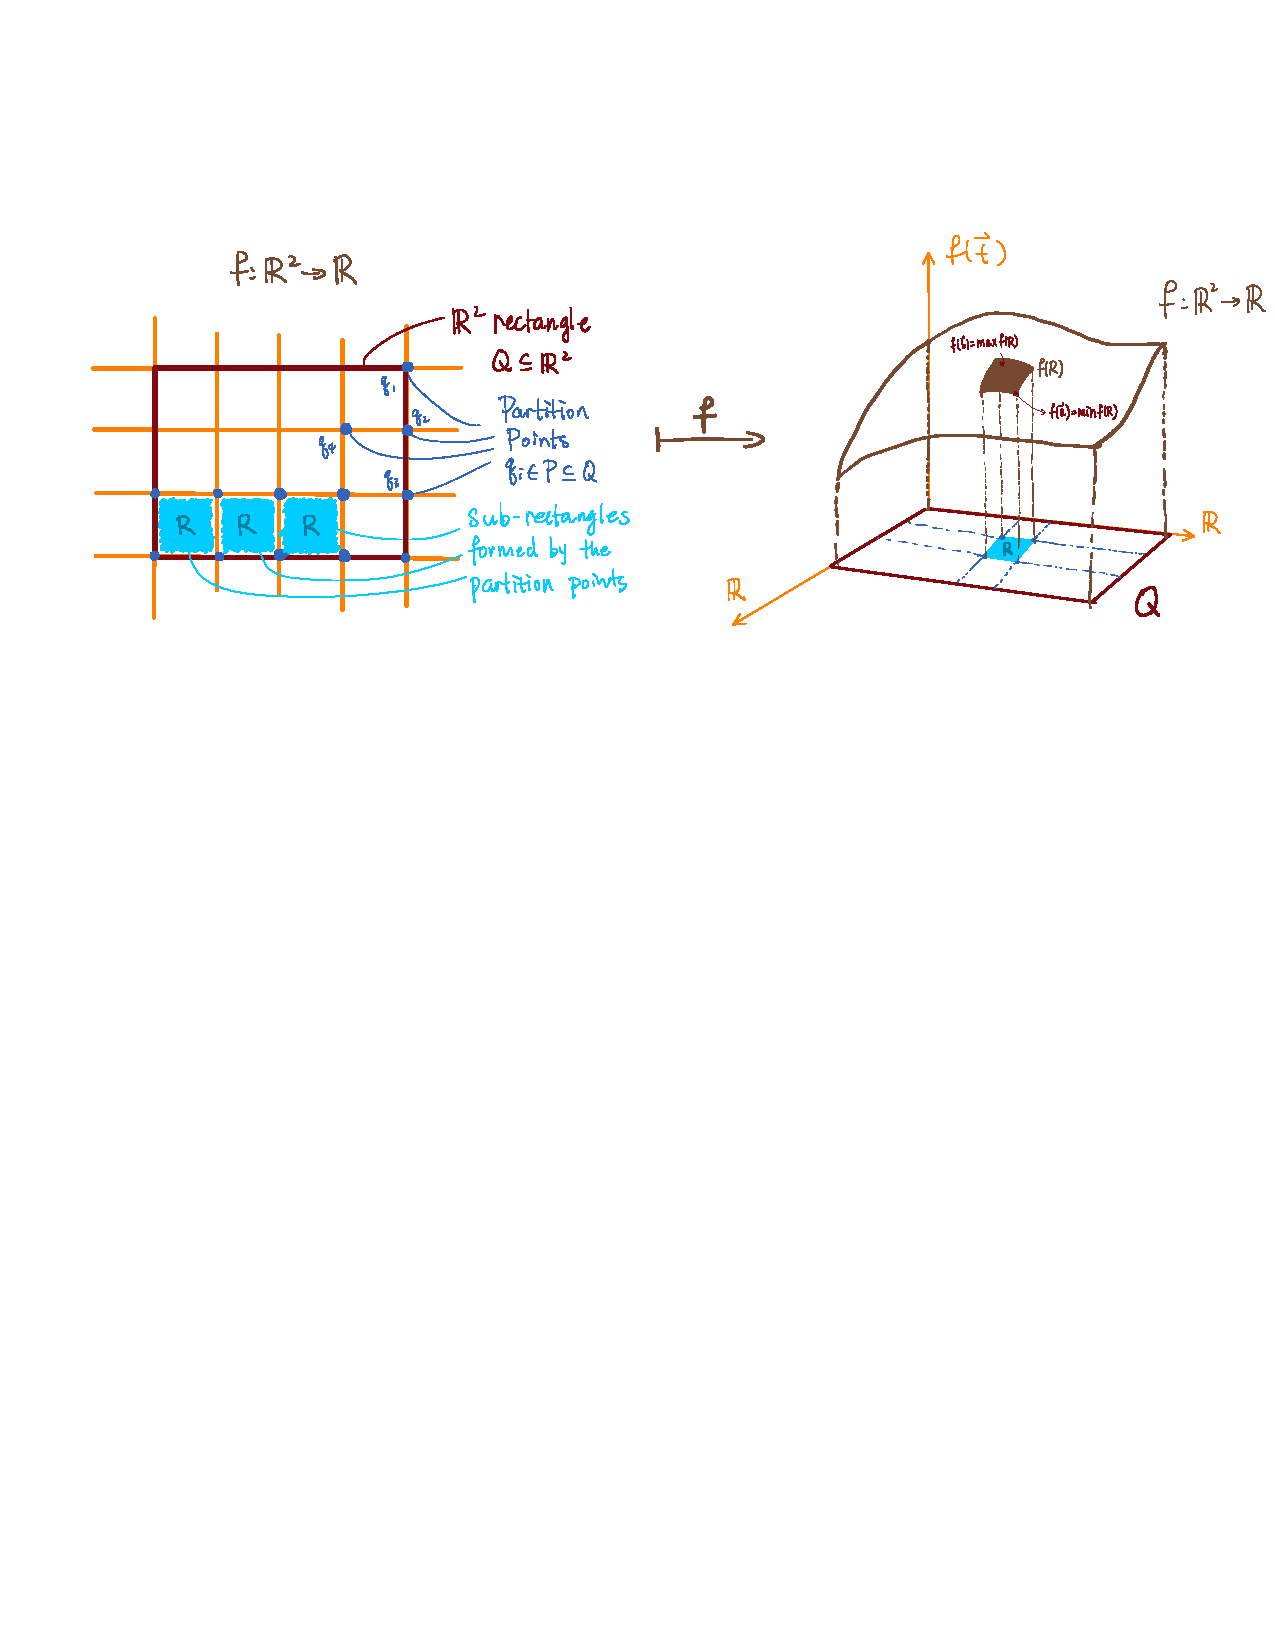
\includegraphics[scale=0.73]{integration.pdf}
\end{center}
We want to fine a way to define the integral $\int_Q$ for bounded functions over $Q$. For $f$ being defined above, bounded function $g:Q \to \R$, and a constant $C \in \R$, $\int_Q$ should satisfies the followings: 

$$\int_Q C = C \cdot V(Q) \qquad\qquad f\leq g \implies \int_Q f \leq \int_Q g \qquad\qquad \int_Q f = \sum_R \int_R f$$

\begin{defn}
For $f:Q \to \R$ with $P$ being a partition of a box $Q\subseteq \R^n$, let $\{R_i\}$ be the set of subboxes of $Q$ determined by $P$, we define the followings:
$$L(f,P) \coloneqq \sum_{R\in \{R_i\}} \left(\inf(f(R))V(R)\right) \qquad\qquad\quad	U(f,P) \coloneqq \sum_{R\in \{R_i\}} \left(\sup(f(R))V(R)\right)$$
\end{defn}

\note From Definition 10.0.0.0.4, it is immediate that $L(f,P) \leq U(f,P)$.

\begin{defn}
Let $P'$ and $P$ be partitions for  a box $Q\subseteq \R^n$, we say $P'$ refines $P$ provided that $P'$ is obtained by adding more partition points to $P$, that is, $P'$ refines $P$ provided that we have $P \subseteq P'$.  
\end{defn}


\begin{lem}
For bounded function $f:Q \to \R$ with $P$ being a partition of a box $Q\subseteq \R^n$, we have:
$$L(f,P) \leq L(f,P') \leq U(f,P') \leq U(f,P)$$
\end{lem}
\begin{proof}
The proof for this Lemma for $n\geq 1$ is on Munkres Lemma 10.1.\\ One might also want to check Spivak pg.255 for $n=1$.
\end{proof}

\begin{lem}
Let $P$ and $P'$ be arbitrary partitions of a box $Q\subseteq \R^n$, and let $f$ be a bounded function from $Q$ to $\R$. Then we have $L(f,P) \leq U(f,P')$. 
\end{lem}
\begin{proof}
First we form a partition $P''$ using all partition points from $P$ and $P'$. Here $P''$ refines $P$ and $P'$. By Lemma 10.0.1, we have the following holds: 
$$L(f,P) \leq L(f,P'') \leq U(f,P'') \leq U(f,P')$$
This completes the proof.
\end{proof}


\begin{defn}
Let $A$ be a subset of $\R$, and let $f:\Power(A) \to \R$ be a bounded function.
$$\inf_{A_i} f(A_i) \coloneqq \inf\{f(A_i) \mid A_i \subseteq A\} \quad\qquad\qquad \sup_{A_i} f(A_i) \coloneqq \sup\{f(A_i) \mid A_i \subseteq A\}$$
\end{defn}

\begin{defn}
Let $P$ be a partition of a box $Q \subseteq \R^n$, and let $f:Q \to \R$ be a bounded function.\\
The Darboux Upper Integral is defined to be:
$$\upint_Q f \coloneqq \inf_P U(f,P)$$
The Darboux Lower Integral is defined to be:
$$\lowint_Q f \coloneqq \sup_P L(f,P)$$
\end{defn}
\newpage

\begin{prop}
For a bounded function $f:Q \to \R$ with $Q$ being a box of $\R^n$, we have the following: 
$$\lowint_Q f \leq \upint_Q f$$
\end{prop}
\begin{proof}
Combining Lemma 1.0.1 with Lemma 10.0.2, the result follows.
\end{proof}

\begin{defn}
For a bounded function $f:Q \to \R$ with $Q$ being a box of $\R^n$, $f$ is said to be Riemann integrable over $Q$ provided that $\lowint_Q f = \upint_Q f$, in which case we write $\int_Q f \coloneqq \lowint_Q f$.
\end{defn}

\begin{thm}[Cauchy Criterion, or Riemann Condition, for Integrability]
For a bounded function $f:Q \to \R$ with $Q$ being a box of $\R^n$, $f$ is Riemann integrable on $Q$ if and only if for all $\epsilon>0$, there exists a partition $P$ such that $U(f,P) < L(f,P) + \epsilon$.
\end{thm}
\begin{proof}
For the $\Leftarrow$ direction, for all $\epsilon>0$, there exists some partition $P$ of $Q$ such that we have:
$$0 \leq \upint_Q f - \lowint_Q f \leq U(f,P) - L(f,P) < \epsilon$$
so we must have $\upint_Q f = \lowint_Q f $ by Lemma 1.0.1, this completes the proof for the $\Leftarrow$ direction. For the $\Rightarrow$ direction, for a given $\epsilon >0$, we see that there exists partitions $P,P'$ of $Q$ with $U(f,P') < L(f,P)+\epsilon$, take refinement $P''$ of $P$ and $P'$, we have $U(f,P'') < L(f,P'')+\epsilon$, the result follows.
\end{proof}


\begin{defn}
Let $Q $ be a box of $\R^n$, the osculation of a bounded function $f:Q \to \R$ at $\vec{a}\in \R^n$ is defined to be the following: 
$$osc(f,\vec{a}) \coloneqq \inf\left\{ \sup\{ f(\vec{t})\mid \vec{t} \in B_\delta(\vec{a})\cap Q\}  - \inf\{ f(\vec{m})\mid \vec{m} \in B_\delta(\vec{a})\cap Q\}  \mid {\delta>0} \right\} $$
\end{defn}

\note Let $f:Q \to \R$ be a bounded function with $Q$ being a box of $\R^n$. $osc(f,\vec{a}) < \epsilon$ if and only if $\exists\ $open neighborhood $U$ of $\vec{a}$ such that $\sup_{U\cap Q} f - \inf_{U\cap Q} f < \epsilon$. Moreover, $\{ \vec{a} \in Q,\ osc(f,\vec{a})<\epsilon\}$ is relatively open, and here $g:Q \to \R \ \ \ \vec{a}\mapsto osc(f,\vec{a})$ is an upper semi-continuous function.\\

\example
$$f: \R \to \R \ \ \ x\mapsto\begin{cases} \sin(1/x) & x \neq 0 \\ 0 & x = 0\end{cases} \qquad\qquad\qquad osc(f,a) = \begin{cases} 0 & a \neq 0 \\ 2 & a = 0 \end{cases}$$

\hfill\break
\begin{defn}
Let $f:Q \to \R$ be a bounded function with $Q$ being a box of $\R^n$. Here we define:
$$\D_k(f)\coloneqq \{ \vec{a} \in Q \mid osc(f,\vec{a}) \geq \frac{1}{k}\}$$
\end{defn}
 
\note The set $\D_k(f)$ defined in Definition 10.1.0.0.2 is closed.

\begin{defn}
Let $f:Q \to \R$ be a bounded function with $Q$ being a box of $\R^n$. $$\D(f) \coloneqq \bigcup_{k=1}^\infty \D_k(f) = \{\vec{a}\in Q \mid f \text{ is not continuous at } \vec{a}\}$$
\end{defn}
\note The set $\D(f)$ defined in Definition 10.1.0.0.3 is an $F_\sigma$ set.

\begin{defn}
Let $(X,\T)$ be a topological space, let $A$ be a subset of $X$ equipped with the subspace topology inherited from $X$, let $M$ be a subset of $A$, the relative interior of $M$, denoted as $\text{rInt}(M)$, is defined to be: $$\text{rInt}(M) \coloneqq \{x\in M \mid \exists\ \epsilon >0,\ s.t.\  B_\epsilon(x)\cap A \subseteq M \}$$
\end{defn}

\begin{defn}
Let $A$ be a subset of $R^n$. $A$ is said to have measure zero in 
$R^n$ provided that, for every $\epsilon > 0$, there exists countably many boxes $Q_1,Q_2,\cdots$ in $R^n$ such that we have $A \subseteq \bigcup_{i=1}^\infty Q_i$ and $\sum_{i=1}^\infty V(Q_i)< \epsilon$. 
\end{defn}


\begin{thm}
Let $f:Q \to \R$ be a bounded function with $Q$ being a box of $\R^n$.\\ Given $\epsilon>0$ and some $k \in \N$, the followings are equivalent:
\begin{enumerate}[topsep=3pt,itemsep=-1ex,partopsep=1ex,parsep=1ex]
\item The function $f$ is Riemann integrable on $Q$
\item There exists a partition $P$ such that $U(f,P) < L(f,P) + \epsilon$
\item There exists some subboxes $R_1,R_2,\cdots, R_j$ of $Q$ such that we have: 
$$\D_k(f) \subseteq R_1\cup R_2\cup\cdots\cup R_j \text{ and } \sum_{i=1}^j V(R_i) <\epsilon$$ 
\item There exists some subboxes $R_p$ of $Q$ such that we have: 
$$\D(f) \subseteq \bigcup_{p=1}^\infty R_p \text{ and } \sum_{p=1}^\infty V(R_p) < \epsilon$$
\item There exists some subboxes $R_p$ of $Q$ such that we have: 
$$\D(f) \subseteq \bigcup_{p=1}^\infty \text{rInt}(R_p) \text{ and } \sum_{p=1}^\infty V(R_p) < \epsilon$$
\end{enumerate}
In the context of this theorem, a box $R$ is called a subbox of $Q$ provided that $R$ is a box in $\R^n$ contained in $Q$, and here $R$ is allowed to have zero volume, or in other words, measure zero.
\end{thm}
\begin{proof}
The equivalency between (1) and (2) is immediate from Theorem 10.1. Now we will show that (2) implies (3). Given $k \in \N$, pick a partition $P$ of $Q$ such that for subboxes $R_i$ determined by $P$, we have the following holds: $$U(f,P) - L(f,P)=\sum_{R_i}\left(\sup_{R_i} f- \inf_{R_i} f\right)V(R) < \epsilon/(19k)$$
Let $R_{i,1},R_{i,2},\cdots, R_{i,l}$ denote the subboxes determined by $P$ that satisfies: 
$$\Int(R_{i,j}) \cap \D_k(f)\neq \emptyset$$ 
Then we can write the following:
\begin{align*}
\frac{1}{k}\sum_{p=1}^l V(R_p) = \sum_{p=1}^l \frac{1}{k} V(R_{i,p}) \leq \sum_{p=1}^l \left(\sup_{R_{i,p}} f - \inf_{R_{i,p}} f\right) V(R_{i,p}) \leq \frac{\epsilon}{19k}
\end{align*}
which implies that we have:
$$\sum_{p=1}^l V(R_{i,p}) < \epsilon$$
Here we note that, $\D_k(f)$ might not necessarily be a subset of $R_{i,1} \cup R_{i,2}\cup\cdots\cup R_{i,l}$ because $\D_k(f)$ might have nonempty intersection with the boundaries of some other subboxes $R_{b,1},R_{b,2},\cdots, R_{b,t}$ determined by $P$, so we can write the following:
$$\D_k(f)\subseteq R_{i,1}\cup R_{i,2} \cup \cdots R_{i,l} \cup\Bd(R_{b,1}) \cup \Bd(R_{b,2}) \cup \cdots \cup \Bd(R_{b,t})$$ 
where each $\Bd(R_{b,j})$ is a finite union of subboxes of $Q$ that have measure zero, hence we have the following: $$\D_k(f) \subseteq R_{i,1}\cup R_{i,2} \cup \cdots R_{i,l} \cup  R_{z,1}\cup R_{z,2} \cup \cdots \cup R_{z,m}$$
for some zero volume subboxes $R_{z,j}$ of $Q$. With the definition of a box in $\R^n$, it follows that we have the following:
$$\sum_{p=1}^l V(R_{i,p}) + \sum_{j=1}^m V(R_{z,j}) = \sum_{p=1}^l V(R_{i,p})< \epsilon$$ 
This shows that (2) implies (3). To show that (3) implies (4), for each $k \in \N$, pick finitely many subboxes of $Q$ such that $\D_k(f)$ is contained in the union of the subboxes and the volume sum of those subboxes is less than $\frac{\epsilon}{2^k}$, the result follows. Now we will show (4) implies (5), let $\epsilon>0$ be given, pick subboxes $R_p$ such that $\D(f) \subseteq \bigcup_{p=1}^\infty R_p$ with $\bigcup_{p=1}^\infty V(R_p) < \frac{\epsilon}{19}$. For each $p$, pick suboxes $\hat{R}_p$ of $Q$ such that we have the following conditions hold: 
\begin{enumerate}[topsep=3pt,itemsep=-1ex,partopsep=1ex,parsep=1ex]
\item If $V(R_p) >0$, then $R_p \subseteq \text{rInt}(\hat{R}_p)$ with $V(\hat{R}_p) < 2V(R_p)$
\item If $V(R_p) = 0$, then $R_p \subseteq \text{rInt}(\hat{R}_p)$ with $V(\hat{R}_p) < \frac{\epsilon}{2^{p+1}}$
\end{enumerate}
Here we get $\sum_{p=1}^\infty V(\hat{R}_p) < 2\cdot \frac{\epsilon}{19} + \sum \frac{\epsilon}{2^{p+1}} < \epsilon$. This shows that (4) implies (5). Lastly, we will show (5) implies (2). Given $\epsilon>0$, let $\hat{\epsilon} =(\epsilon)/(3(M+V(Q)))$ where $M = \max(|f||_Q)$. By assumption, there exists some suboxes $R_p$ such that we have $\D(f) \subseteq \bigcup_{p=1}^\infty \text{rInt}(R_p)$ with $\sum V(R_p)<\hat{\epsilon}$. For each $\vec{a}\in Q \setminus \D(f)$, $f$ is continuous at $\vec{a}$, so there exists a subbox $Q_{\vec{a}}$ of $Q$ with $\vec{a}\in \text{rInt}(Q_{\vec{a}})$ and $|f(\vec{x}) - f(\vec{a})| < \hat{\epsilon}$ for $\vec{x}\in Q_{\vec{a}}$. Note here $Q \subseteq \bigcup_{p=1}^\infty \text{rInt}(R_p) \cup (\bigcup_{\vec{a}\in Q\setminus \D(f)} \text{rInt}(Q_{\vec{a}}))$. Here we note that $Q$ is compact, and each $\text{rInt}(Q_{\vec{a}})$, or $\text{rInt}(R_p)$, is open, so there exists a finite subcover such that we have the following:
$$Q \subseteq \left(\bigcup_{p=1}^s \text{rInt}(R_{p})\right) \cup \left( \bigcup_{\text{finitely many }\vec{a}\in Q\setminus \D(f)} \text{rInt}(Q_{\vec{a}}) \right)$$
Here we write the followings:
$$\text{rInt}(Q_{\vec{a}_1}) \cup \text{rInt}(Q_{\vec{a}_2}) \cup \cdots \cdot \text{rInt}(Q_{\vec{a}_t}) = \bigcup_{\text{finitely many }\vec{a}\in Q\setminus \D(f)} \text{rInt}(Q_{\vec{a}}) $$
$$\text{rInt}(R_{p_1})\cup \text{rInt}(R_{p_2})\cup \cdots, \cup \text{rInt}(R_{p_s}) = \bigcup_{p=1}^s \text{rInt}(R_{p})$$ 
Pick partition $P'$ such that each subbox $R$ determined by $P'$ satisfies at least one of the two conditions:
(1) $R \subseteq Q_{\vec{a}_j}$, or
(2) $R \subseteq R_{p_k}$.
If $R$ satisfies condition (1), we say $R$ is good, and if $R$ does not satisfies (1), we say $R$ is bad. Then we can write the following:
\begin{align*}
U(f,P) - L(f,P) &= \sum_{R} (\sup_{R} f - \inf_R f) V(R)\\
&= \sum_{good\ R}(\sup_{R} f - \inf_R f) V(R) + \sum_{bad\ R} (\sup_{R} f - \inf_R f) V(R)\\ &\leq \sum_{good\ R} 2\hat{ \epsilon}(R)  + \sum_{bad \ R}2MV(R)\\ &\leq 2\hat{\epsilon}V(Q) + 2M\hat{\epsilon} \\&< \epsilon
\end{align*}
This shows that (5) implies (2). Now we have shown that (2), (3), (4), (5), are equivalent, and we know that (1) and (2) are equivalent by Theorem 10.1, this completes the proof of Theorem 10.2. 
\end{proof}

\begin{lem}
Let $f:Q \to \R$ and $g:Q \to \R$ be function defined on a box $Q \subseteq \R^n$. If we have $f(\vec{x})\leq g(\vec{x})$ for all $\vec{x}$ in $Q$, then we have $\lowint_Q f \leq \lowint_Q g$ and $\upint_Q f \leq \upint_Q g$.
\end{lem}
\begin{proof}
For partition $P$ of the box $Q$, we have $L(f,P) \leq L(g,P) \leq \lowint_Q g$, it follows that $\lowint_Q f \leq \lowint_Q g$. On the  other hand, we have  $\upint_Q f \leq U(f,P) \leq U(g,P)$, it follows that $\upint_Q f \leq \upint_Q g$. A more detailed proof can be found on Section 10 on Munkres. 
\end{proof}

\begin{thm}[Fubini's Theorem]
Let $A$ be a box in $\R^k$, $B$ be a box in $\R^n$, let $Q = A \times B$, and let $f:Q \to \R$ be a bounded function. Then we can write:
$$\lowint_Q f  \leq \lowint_{\vec{x}\in A} \lowint_{\vec{y}\in B}f(\vec{x},\vec{y})\leq \ \ \ \begin{cases}\begin{rcases} \lowint_{\vec{x}\in A} \upint_{\vec{y} B}f(\vec{x},\vec{y}) \\ \upint_{\vec{x}\in A} \lowint_{\vec{y}\in B}f(\vec{x},\vec{y})\ \  \end{rcases}\end{cases}\leq  \upint_{\vec{x}\in A} \upint_{\vec{y}\in B}f(\vec{x},\vec{y})\leq  \upint_Q f$$
\end{thm}
\begin{proof}
By Proposition 10.0.3, we know that $\lowint_Q f \leq \upint_Q f$, we will refer this result as (*). By Lemma 10.2.1, we know that $\lowint_Q f \leq \lowint_Q g$ when $f(\vec{x})\leq g(\vec{x})$ for all $\vec{x}\in Q$, we refer this result as (a). Also by Lemma 10.2.1, we know that $\upint_Q f \leq \upint_Q g$ when $f(\vec{x})\leq g(\vec{x})$ for all $\vec{x}\in Q$, we refer this result as (b). Here we see that, Using result from (*), we get $\lowint_{\vec{x}\in A} \lowint_{\vec{y}\in B} f(\vec{x},\vec{y}) \leq \upint_{\vec{x}\in A} \lowint_{\vec{y}\in B} f(\vec{x},\vec{y})$, and $\lowint_{\vec{x}\in A} \upint_{\vec{y}\in B} f(\vec{x},\vec{y}) \leq \upint_{\vec{x}\in A} \upint_{\vec{y}\in B} f(\vec{x},\vec{y})$. Combining the result from (*) and (a), we get $\lowint_{\vec{x}\in A} \lowint_{\vec{y}\in B} f(\vec{x},\vec{y}) \leq \lowint_{\vec{x}\in A} \upint_{\vec{y}\in B} f(\vec{x},\vec{y})$. Combining the result from (*) and (b), we get $\upint_{\vec{x}\in A} \lowint_{\vec{y}\in B} f(\vec{x},\vec{y}) \leq \upint_{\vec{x}\in A} \upint_{\vec{y}\in B} f(\vec{x},\vec{y})$. To show $\lowint_Q f \leq \lowint_{\vec{x}\in A} \lowint_{\vec{y}\in B}f\left(\vec{x},\vec{y}\right)$, we denote $\vec{x}_0 \in R_A$ where $R_A$ is a subrectangle of $A$, denote $R_b$ as subrectangle of $B$, we can write: $$\lowint_{\vec{y}\in B} f\left(\vec{x}_0, \vec{y}\right) \geq \sum_{R_B} \inf_{\vec{y}\in R_B} \left(f\left(\vec{x}_0,\vec{y}\right)\right) \cdot V\left(R_B\right) \geq \sum_{R_B} \inf_{R_A \times R_B}\left(f\right)\cdot V\left(R_B\right) $$
On the other hand, we have:
\begin{align*}
\lowint_{\vec{x}\in A }\left(\lowint_{\vec{y}\in B} f\left(\vec{x},\vec{y}\right)\right) &\geq  \sum_{R_A} \inf_{\vec{x}\in R_A} \left(\lowint_{\vec{y}\in B}f\left(\vec{x},\vec{y}\right)\right) V\left(R_A\right)\\
&\geq \sum_{R_A}\sum_{R_B} \inf_{R_A\times R_B} \left(f\right) V\left(R_A \times R_B\right) \\
&= L\left(f,P\right)
\end{align*}
Hence we see that $\lowint_Q f \leq \lowint_{\vec{x}\in A} \lowint_{\vec{y}\in B} f(\vec{x},\vec{y})$. Lastly, one can show that we have $\upint_{\vec{x}\in A} \upint_{\vec{y}\in B} f(\vec{x},\vec{y}) \leq \upint_Q f$ by combining $\lowint_Q f \leq \lowint_{\vec{x}\in A} \lowint_{\vec{y}\in B} f(\vec{x},\vec{y})$ with the fact that $\upint_Q f = -\lowint_Q  (-f)$.  This completes the proof of this theorem.
\end{proof}

\begin{corT}
Let $A$ be a box in $\R^k$, $B$ be a box in $\R^n$, let $Q = A \times B$, and let $f:Q \to \R$ be a bounded function. If $f$ is integrable on $Q$, then we have:
$$\lowint_Q f  = \lowint_{\vec{x}\in A} \lowint_{\vec{y}\in B}f(\vec{x},\vec{y})= \ \ \ \begin{cases}\begin{rcases} \lowint_{\vec{x}\in A} \upint_{\vec{y} B}f(\vec{x},\vec{y}) \\ \upint_{\vec{x}\in A} \lowint_{\vec{y}\in B}f(\vec{x},\vec{y})\ \  \end{rcases}\end{cases}= \upint_{\vec{x}\in A} \upint_{\vec{y}\in B}f(\vec{x},\vec{y})=  \upint_Q f$$ 
and we can write:
$$\int_Q f = \int_{\vec{x}\in A}\upint_{\vec{y}\in B}f(\vec{x},\vec{y}) = \int_{\vec{x}\in A}\lowint_{\vec{y}\in B} f(\vec{x},\vec{y})$$
\end{corT}
\note Given the settings in Corollary 10.3.1, $\int_{\vec{y}\in B} f(\vec{x},\vec{y})$ may not necessarily exist. 



\begin{corT}
A function $f$ is continuous on $Q = I_1 \times I_2 \times \cdots \times I_n$ implies the following:
$$\int_Q f = \int_{x_1\in I_1}  \int_{x_{n-1} \in I_{n-1}} \int_{x_n \in I_n} f(x_1,\cdots, x_n)$$
\end{corT}


\begin{lem}
Let $R$ be a subbox of a box $Q\in \R^n$. \\
For $y > V(R)$, there exists a subbox $\hat{R}$ of $Q$ with $R \subseteq \text{rInt}(\hat{R}) \subseteq Q$ such that $V(\hat{R})<y$. 
\end{lem}

\note Consider a bounded function defined on a box $Q$.
\begin{enumerate}[topsep=3pt,itemsep=-1ex,partopsep=1ex,parsep=1ex]
\item If $f^{-1}(0)$ is dense in $Q$, then all $L(f,P) \leq 0$, all $U(f,P) \geq 0$, which implies: $$\lowint_Q f \leq 0 \leq \upint_Q f$$
\item If $f^{-1}(0)$ is dense in $Q$ and $f$ is integrable, then $\int_Q f = 0$.
\item If $f \geq 0$, $f(\vec{a}) > 0$, and $\lowint_Q f =0$, then $f$ is discontinuous.
\item If $f \geq 0$, $f$ is integrable on $Q$, and $\int_Q f = 0$, then $Q \setminus f^{-1}(0)$ has measure zero. 
\item If $f \geq 0$, $f(\vec{a}) > 0$, $f $ is continuous at $\vec{a}$, then $\lowint_Q f > 0$. 
\end{enumerate}
\begin{proof}[Proof of (5)]
Choose partition $P$ such that $f > \frac{f(\vec{a})}{2}$ on some boxes $R^*$ determined by $P$. Then we can write the following:
$$\lowint_Q f \geq L(f,P) = \inf_{R^*} (f)\cdot V(R^*) + \sum_{R} \inf_R f\cdot V(R) \geq \frac{f(\vec{a})}{2}V(R^*)+ 0 $$
This completes the proof.
\end{proof}

\example Let $Q = [-1,1] \times [-1,1]$, and $f = \mathbb{I}_{\{0\} \times \Q}$, where $\mathbb{I}$ is the indicator function, we see that $\D(f) = \{0\} \times [-1,1]$, which is a set that has zero measure, so we know that $f$ is integrable on $Q$. Notice that, integrating over $y$ with fixed $x$, we have the followings:
$$\upint_{y \in [-1,1]} f(x,y)  = \begin{cases} 
0& x\neq 0 \\ 1 & x = 0
\end{cases} \qquad \qquad \qquad \lowint_{y \in [-1,1]} f(x,y) = \begin{cases} 0 & x \neq 0 \\ 0 & x= 0 \end{cases}$$
One might also integrate over $x$ with fixed $y$ and get $\int_{x \in [-1,1]} f(x,y) = 0$. From Fubini's Theorem, we can write $\int_Q f = 0$. \\




\newpage
\section[Integrating Over a Bounded Set]{\color{red} Integrating Over a Bounded Set \color{black}}


\begin{defn}
Let $S$ be a bounded subset of $\R^n$, and let $f:S \to \R$ be a bounded function.
$$f_S : \R^n \to \R \qquad \vec{x}\mapsto \begin{cases}f(\vec{x}) & \vec{x} \in S \\ 0 &\vec{x}\notin S\end{cases} \qquad \qquad\int_S f \coloneqq \int_Q f_S \quad \text{for box } Q \text{ that contains }S$$
\end{defn}

\begin{prop}
Let $S$ be a bounded subset of $\R^n$, and let $f:S \to \R$ be a bounded function. The existence and the value of $\int_Q f_S$ does not depend on the choice of the box $Q$ which contains $S$.
\end{prop}


\begin{proof}
For the existence of $\int_Q f_S$, let $Q_1,Q_2$ be boxes that contain $S$, and let $Q_3$ be a box of $S$ such that $Q_1$ and $Q_2$ are contained in the interior of $Q_3$. 

\begin{center}
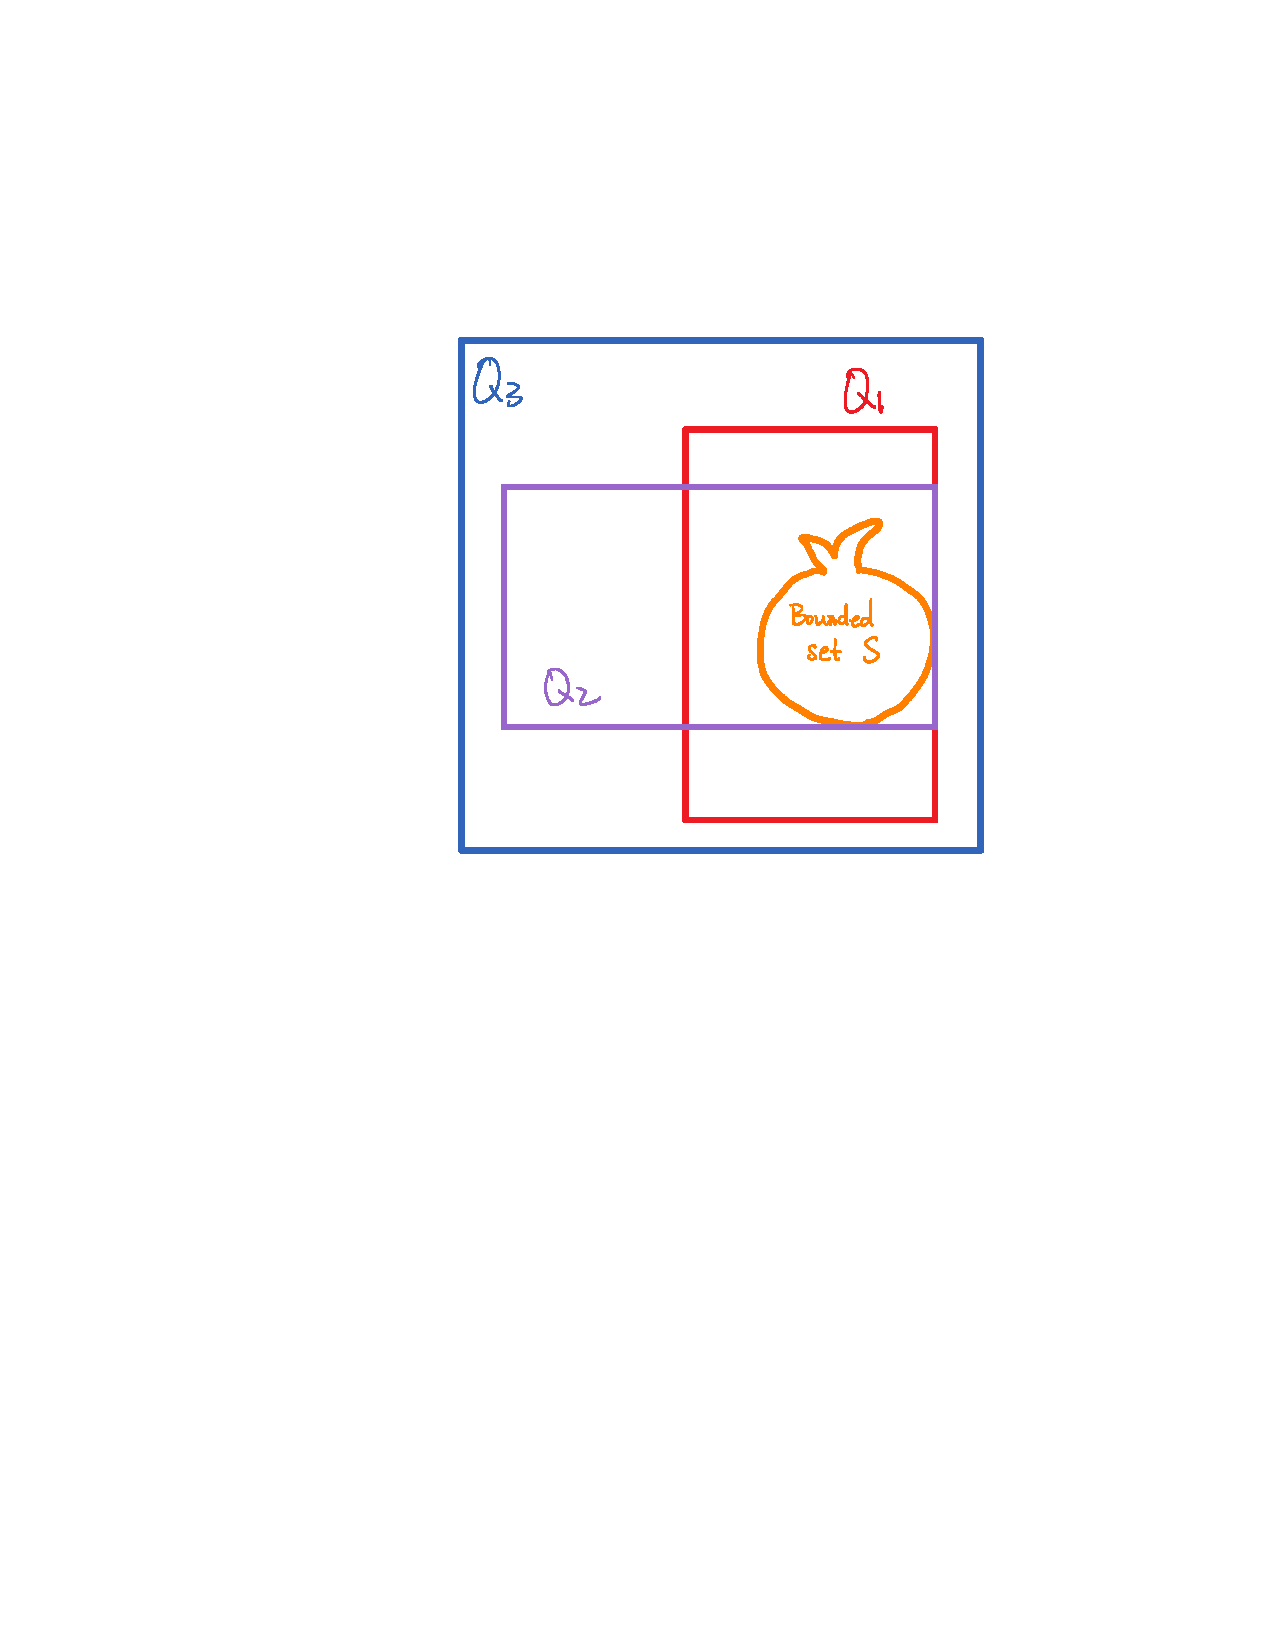
\includegraphics[scale=0.6]{IntOverBddSet.pdf}
\end{center}

We will investigate $\D(f_S)$ on $Q_3$, denoted as $\D(f_S)_3$, and $\D(f_S)$ on $Q_1$, denoted as $\D(f_S)_1$. We see that $\D(f_S)_3 = \D(f_S)_1 \cup \{ \text{subset of }\Bd(Q_1)\}$, here $\{ \text{subset of }\Bd(Q_1)\}$ can be covered by finitely many zero-volume boxes. Here we conclude that $f_S$ is integrable on $Q_1$ if and only if $f_S$ is integrable on $Q_3$ by Theorem 10.2, and similarly, $f_S$ is integrable on $Q_2$ if and only if $f_S$ is integrable on $Q_3$. Now we can conclude that $f_S$ is integrable on $Q_1$ if and only if $f_S$ is integrable on $Q_2$. That is, the integrability of $f_S$ does not depend on the choice of $Q$. Now we will show that $\int_{Q_1} f_S = \int_{Q_3} f_S$. Let $P $ be a partition of $Q_3$, and refine $P$ to $P'$ such that $Q_1$ is contained in a finite union of boxes determined by $P'$. We denote the boxes determined by $P'$ as $P'-$boxes. Then $L(f_S,P) \leq L(f_S, P')$, and we can write the following:
\begin{align*}
L(f_S, P')&= \sum_{\substack{P' \text{-boxes } R  \\ \text{ contained in } Q_1}} \inf_R (f_S) V(R) \quad + \sum_{\substack{\text{other }P'\text{-boxes } R' \\ \text{ contained in }Q \setminus \text{rInt}(Q_1)}} \inf_{R' }(f_S) V(R') \leq \lowint_{Q_1} f_S
\end{align*}
Here we can take the supremum over choice of $P$ to get $\int_{Q_3} f_S \leq \int_{Q_1} f_S$. With similar argument, we get $\int_{Q_3} f_S \geq \int_{Q_1} f_S$ using $U(f_S,P)$, and the result follows. 
\end{proof}
\newpage

\note The proof of the followings can be found on Section 13 in Munkres, and Chapter 13 in Spivak. Let $S\subseteq \R^n$ be bounded, let $a,b \in \R$, and let $f:Q \to \R$ and $g:Q \to \R$ be integrable functions.
\begin{enumerate}[topsep=3pt,itemsep=-1ex,partopsep=1ex,parsep=1ex]
\item $\int_S(af+bg) = a\int_S f + b\int_S g$
\item If $f(\vec{x})\leq g(\vec{x})$ for all $\vec{x}\in S$, then we have $\int_S f \leq \int_S g$
\item $|f|$ is integrable on $S$
\item If $f_S$ is continuous, then $|f|_S$ is continuous. 
\item $|\int_S f| = \max\{ (\int_S f),\ (- \int_S f)\} \leq \int_S |f|$
\item Let $T \subseteq S$, if $f(\vec{x}) \geq 0$ for all $\vec{x}\in S$,  and $f$ is integrable on $T$, then $\int_T f \leq \int_S f$. 
\item If $f$ is integrable on bounded sets $S_1$ and $S_2$, then $f$ is integrable on $S_1 \cup S_2$ and $S_1 \cap S_2$, with the following holds: $$\int_{S_1\cup S_2} = \int_{S_1} f + \int_{S_2} f - \int_{S_1\cap S_2} f$$
\end{enumerate}
\begin{proof}[Proof of (7)]
Let $A = \{ (x,y) \in \R^2 \mid x=0 \text{ or }y=0 \text{ or }x=y\}$. \\Let $\phi:A \to \R$ be a function defined by:
$$\phi:A \to \Q \qquad \begin{cases}(x,0) \mapsto x \\ (0,y) \mapsto y \\ (x,x) \mapsto x    \end{cases}$$
It is easy to check that $\phi$ is continuous, and we have $\phi(f_{S_1}, f_{S_2}) = f_{S_1\cup S_2}$, so we know that $f_{S_1\cup S_2} $ is continuous at the points where $f_{S_1}$ and $f_{S_2}$ are continuous. The discontinuous sets for $f_{S_1}$ and $f_{S_2}$ satisfies the condition of Theorem 10.2 because $f$ is integrable on $S_1$ and $S_2$, then it follows that the discontinuous set for $f_{S_1\cup S_2}$ also satisfies the condition in Theorem 10.2, and hence $f_{S_1\cup S_2}$ is integrable on $S_1 \cup S_2$, where one can easily show that $f_{S_1\cup S_2}+ f_{S_1\cap S_2} = f_{S_1} + f_{S_2}$. 
\end{proof}


\exercise Let $S = \{(x_1,x_2,x_3) \mid x_1 \geq 0,\ x_2\geq 0,\ x_3 \geq 0,\ x_1+x_2+x_3 \leq 1 \}$, here $S$ is a tetrahedron, or a $3$-simplex, with $S = ch( \vec{e}_1,\vec{e}_2,\vec{e}_3,\vec{0})$. Let $Q = [0,1]\times[0,1]\times[0,1]\supset S$, we have the following: 
\begin{align*}
\int_S 1 = \int_{Q} \mathbb{I}_S 
&= \int_{0\leq x_1\leq 1} \int_{0\leq x_2 \leq 1} \int_{0\leq x_3 \leq 1} \mathbb{I}_S 
\\&= \int_{0\leq x_1 \leq 1} \int_{0\leq x_2 \leq 1} \max\{ 1-x_1-x_2, 0\} 
\\&= \int_{0 \leq x_1 \leq 1} \int_{0 \leq x_2 \leq 1-x_1} 1-x_1-x_2
\\&= \int_{0\leq x_1 \leq 1} \left[(1-x_1) x_2 - \frac{x_2^2}{2}\right]^{x_2 = 1-x_1}_{x_2 = 0}
\\&= \int_{0\leq x_1 \leq 1} \frac{(1-x_1)^2}{2} = \left[-\frac{(1-x_1)^3}{2}\right]_{x_1 = 0}^{x_1=1} = \frac{1}{6}
\end{align*}


\newpage
\begin{defn}
Let $E$ be a subset of $\R^n$. $$m^*(E) \coloneqq  \inf\left\{\sum_{j=1}^\infty V(Q_j) \mid E \subseteq \bigcup_{j=1}^\infty Q_j, \text{ where } Q_j \text{ are boxes in }\R^n \right\} $$
Here $m^*(E)$ is called the outer Lebesgue measure of $E$.
\end{defn}

\note A set $E$ has outer Lebesgue measure $0$ provided that $m^*(E) = 0$, if and only if $E$ has measure $0$ as described in Munkres Section 11 and Math 395 IBL. \\

\remark Here we do not allow arbitrary coverage by boxes to avoid having $m^*(E) \equiv 0$.\\

\remark Here we allow infinite coverings. We might consider building the theory using finite coverings, called the outer Jardon measure, defined by the following when $E\subseteq \R^n$ is bounded:
$$m^{*,J}(E) \coloneqq  \inf\left\{\sum_{j=1}^k V(Q_j) \mid E \subseteq \bigcup_{j=1}^k Q_j, \text{ where } Q_j \text{ are boxes in }\R^n \right\} $$
and setting $m^{*,J}(E) \coloneqq \infty$ when $E$ is unbounded. \\


\note For a set $E\subseteq \R^n$, we have $m^*(E) \leq m^{*,J}(E)$.
\begin{prop}
For sets $E_j\subseteq \R^n$.\\ If $m^*(E_j) = 0$ for $j=1,2,\cdots$, then we have $m^*(\bigcup_{j=1}^\infty E_j) = 0$. \\If $m^{*,J}(E_j) = 0$ for $j=1,2,\cdots$, then we have $m^{*,J}(\bigcup_{j=1}^\infty E_j) = 0$.
\end{prop}
\begin{proof}
The proof of this proposition is given on Munkres Theorem 11.1.
\end{proof}


\begin{lem}
For $E \subseteq \R^n$, we have: 
$$m^*(E) = \inf\left\{\sum_{j=1}^\infty V(Q_j) \mid E \subseteq \bigcup_{j=1}^\infty \text{Int}(Q_j) , \text{ where } Q_j \text{ are boxes in }\R^n \right\}$$
$$m^{*,J}(E) = \inf\left\{\sum_{j=1}^k V(Q_j) \mid E \subseteq \bigcup_{j=1}^k \text{Int}(Q_j ), \text{ where } Q_j \text{ are boxes in }\R^n\right\} $$
here we use relative interior when appropriate. 
\end{lem}
\begin{proof}
Comparing to the definition of the Lebesgue and Jardon measure, such restrictions in this Lemma can only increase the infimum. Hence we need to show no increase in the infimum occurs. For the case $m^*(E) = \infty$, the result follows trivially. Let $\epsilon>0$ be given, for nonempty $E$, pick $\widetilde{Q}_j \supseteq \text{Int}(\widetilde{Q}_j) \supseteq Q_j$ with $V(\widetilde{Q}_j) < V(Q_j) + \frac{\epsilon}{2^j}$, by Lemma 10.3.3, here we get $\text{Int}(\widetilde{Q}_j)$ covering $E$ with $\sum V(\widetilde{Q}_j) < \sum V(Q_j) + \epsilon$. Since $\epsilon$ is arbitrary, we see that there is no change in infimum. 
\end{proof}
\newpage

\begin{prop}
Let $K$ be a compact subset of $\R^n$, then we have $m^{*,J}(K) = m^*(K)$
\end{prop}
\begin{proof}
It suffices to show that $m^*(K) \geq m^{*,J}(K)$ holds. Pick $Q_j$ with $\bigcup_{j=1}^\infty \text{Int}(Q_j) \supseteq K$. By compactness of $K$, there exists $M \in \N$ such that $\bigcup_{j=1}^M \Int(Q_j) \supseteq K$, then we can write the following:
$$\sum_{j=1}^\infty V(Q_j) \geq \sum_{j=1}^M V(Q_j) \geq m^{*,J}(K)$$
Now take infimum over choice of $Q_j$'s to get the desired result.
\end{proof}


\note In general, $m^{*,J}(E) \neq m^{*} (E)$ for $E \subseteq \R^n$.\\
\example Let $E = Q \cap [0,1]$, we have $m^*(E) = 0 \neq m^{*,J}(E) = 1$. 



\begin{defn}
Let $S$ be a bounded subset of $\R^n$, let $f:S \to \R$ be a bounded function. $$f_S: \R^n \to \R \ \ \ \vec{x}\mapsto\begin{cases} f(\vec{x}) & \vec{x}\in S \\ 0 & \vec{x}\notin S\end{cases}$$ 
The function $f$ is said to be Riemann integrable on $S$ provided that the function $f_S$ is Riemann integrable on a box $Q$ that contains $S$. 
\end{defn}


\begin{thm}
Let $S$ be a bounded subset of $\R^n$, let $f:S \to \R$ be a bounded continuous function, let $E = \{ \vec{x}_0 \in \Bd(S) \mid\lim_{\vec{x}\in S,\ \vec{x}\to \vec{x}_0} f(\vec{x}) \neq 0 \}$. If we have $m^*(E) = 0$, then $f$ is Riemann integrable on $S$. 
\end{thm}
\begin{proof}
Note that $E$ also contains isolated points of $S$, and for such isolated point $\vec{p}$, if exists, $\exists\ \epsilon >0$ such that $\#(B_\epsilon(\vec{p}) \cap S) = 1$, and $\vec{p}\notin \D(f_S)$. Here we have $\D(f_S) \subseteq E$, the result follows immediately from Theorem 10.2. 
\end{proof}

\begin{corT}
Let $S$ be a bounded subset of $\R^n$, let $f:S \to \R$ be a bounded continuous function.\\ 
If $m^*(\Bd(S)) = 0$, then $f$ is Riemann integrable on $S$. 
\end{corT}

\begin{defn}
A bounded set $S \subseteq \R^n$ is said to be rectifiable provided that one of the following holds:
\begin{enumerate}[topsep=3pt,itemsep=-1ex,partopsep=1ex,parsep=1ex]
\item The function $\mathbb{I}:S \to \R \ \ \ \vec{x}\mapsto 1$ is Riemann integrable on $S$
\item The indicator function $\mathbb{I}_S$ is integrable on some box $Q\subseteq \R^n$ that contains $S$
\item $m^*(\Bd(S)) = 0$
\item $m^{*,J}(\Bd(S)) = 0$
\end{enumerate} 
\end{defn}
\note By Corollary 10.4.1, if a bounded set $S\subseteq \R^n$ is rectifiable, then all bounded continuous functions defined on the set $S$ are integrable.

\begin{defn}
Let $S\subseteq \R^n$ be a rectifiable set, let $\mathcal{I}:S \to \R \ \ \ \vec{x}\mapsto 1$. $V(S) \coloneqq \int_{S} \mathcal{I}$.
\end{defn}


\note Let $S\subseteq \R^n$ be a rectifiable set, let $A = \Int(S)$. Then we have $\Bd(A) \subseteq \Bd(S) \ \Rightarrow  m^*(\Bd(A)) \leq m^*(\Bd(S)) = 0\ \Rightarrow A$ is rectifiable $\Rightarrow \mathbb{I}_S$ and $\mathbb{I}_A$ are integrable, where $\mathbb{I}_S,\,\mathbb{A}$ are indicator functions on $S$ and on $A$. Moreover, $\mathbb{I}_{S\setminus A}= \mathbb{I}_S - \mathbb{I}_A$ is integrable on a box $Q$ that contains $\bar{S}$ $\Rightarrow S\setminus A$ is rectifiable, $\Int(S\setminus A) = \emptyset$, for all partition $P$, $L(\mathbb{I}_{S\setminus A}, P) = 0 \ \Rightarrow\ \int_Q \mathbb{I}_{S\setminus A} = 0\ \Rightarrow \ \int \mathbb{I}_A = \int \mathbb{I}_S\  \Rightarrow \ V(A) = V(S)$. \\


\newpage
\section[Extended Riemann Integrals]{\color{red}Extended Riemann Integrals \color{black}}

In this section we will discuss the integrability of a function $f$ defined on a set $S\subseteq \R^n$, not necessarily bounded, with the property that $f$ is not necessarily bounded. We will focus on discussing the integrability of a continuous real-valued function $f$ defined on an open set $A\subseteq \R^n$, with $A$ and $f$ being not necessarily bounded. \textbf{We will start by assuming that $f(\vec{a}) \geq 0$ for all $\vec{a}\in A$.}

\begin{defn}
Let $A$ be an open subset of $\R^n$, and let $f:A \to \R$ be a continuous function with $f(\vec{a}) \geq 0,\ \forall\vec{a}\in A$, we define the Extended Riemann Integral of $f$ on $A$ as the following:
$$ext \int_A f \coloneqq \sup\left\{ \int_E f  \mid E \text{ is a compact rectifiable set that is contained in } A\right\}$$
\end{defn}

\begin{lem}
Let $A$ be an open subset of $\R^n$ and let $B$ be an open subset of $A$, then $ext \int_B f  \leq ext \int_A f$ for non-negative function $f$ defined on $A$ and on $B$. 
\end{lem}

\begin{defn}
For bounded open set $A\subseteq \R^n$ and bounded non-negative continuous function $f$ defined on $\R^n$. For a box $Q$ that contains $A$, we define the following: $$\lowint_A f \coloneqq \lowint_Q f_A$$ 
\end{defn}

\note For bounded open $A\subseteq \R^n$ and bounded non-negative continuous function $f$ defined on $\R^n$, we have the followings:
\begin{enumerate}[topsep=3pt,itemsep=-1ex,partopsep=1ex,parsep=1ex]
\item When $A$ is rectifiable, then $\int_A f$ exists.
\item For compact rectifiable subset $E$ of $A$, we have:
$$\int_E f = \lowint_E f \leq \lowint_A f \qquad \Rightarrow \qquad ext \int_A f \leq \lowint_A f$$
\item Let $P$ be a partition of a box $Q$ that contains $A$, let $M$ be the union of all the boxes determined by $P$ that are contained in $A$, we have $$L(f_A, P ) \leq \int_{M} f \leq ext \int_A f
\qquad \Rightarrow\qquad \lowint_A f \leq ext \int_A f$$
\item Combining (2) and (3) we have $\lowint_A f = ext \int_A f$.
\item From (4), we conclude that if $f$ is integrable on $A$, then $\int_A f = ext\int_A f$
\end{enumerate}

\begin{lem}[Computational Methods for Extended Riemann Integral]
Let $E_1\subseteq E_2\subseteq \cdots \subseteq A\subseteq \R^n$ with each $E_j$ being compact rectifiable, $\bigcup_j \Int(E_j) = A$, and $A$ being open. We have $ext \int_A f = \lim_{j \to \infty} \int_{E_j} f$ for any non-negative continuous function $f:\R^n \to \R$. 
\end{lem}
\begin{proof}
We have each of $\int_{E_j} f \leq ext\int_A f$. So $\lim_{j\to \infty} \int_{E_j} f \leq ext \int_A f$. If $E\subseteq A$ is compact rectifiable, then by the compactness of $E$, we have $E\subseteq E_M$ for some $M$, because $E\subseteq \Int (E_1) \cup \Int(E_2) \cup \cdots \cup \Int(E_M) = \Int (E_M) \subseteq E_M$. Here we can write that $\int_E f \leq \int_{E_M} f \leq \lim_{j \to \infty} \int_{E_j} f$, so we have $ext \int_A f \leq \lim_{j \to \infty} \int_{E_j} f$. We have proved both directions, the result follows.
\end{proof}
\note Given the setting in Lemma 12.0.2. It is not automatic to have $\bigcup E_j = A$. As an example, consider $E_j = [-j,0] \cup [\frac{1}{j},j]$, we have $\bigcup E_j = \R$, and $\bigcup \Int(E_j) = \R\setminus \{0\}$. 

\begin{prop}
For open subset $A$ of $\R^n$. One can always find $E_j$ that satisfies $E_1\subseteq E_2\subseteq E_3\subseteq \cdots \subseteq A$ with each $E_j$ being compact rectifiable, and $\bigcup_j \Int(E_j) = A$.
\end{prop}
\begin{proof}
One might propose a proof that is similar to the proof of Lemma 15.1 on Munkres. Alternatively, one can construct each $E_j$ by letting $E_j$ be the union of all closed hyper cubes, where each cube has side length $\frac{1}{2^{j}}$, each cube is a subset of $A$, and the vertex of each cube has coordinates in $\frac{\Z}{2^j} \cap [-j, j]$.
\end{proof}

\hfill\break
\example $$\int_\R \frac{1}{1+x^2} = \lim_{j \to \infty} \int_{\{x \mid -j \leq x \leq j\}}\frac{1}{1+x^2} = \lim_{j\to \infty} \arctan(x)]_{x=-j}^{x=j} = \lim_{j \to \infty} 2\arctan(j) = \pi$$

\hfill\break
\example 
\begin{align*}
\int_{\R^2} \frac{1}{1+x^2+y^2} &= \lim_{j\to \infty} \int_{\{x \mid -j \leq x\leq j\}\times \{y \mid  -j\leq y \leq j\}} \frac{1}{1+x^2+y^2} \\
&= \lim_{j\to \infty} \int_{\{y \mid -j\leq y \leq j\}} \int_{\{x \mid -j \leq x\leq j\}} \frac{1}{1+x^2+y^2} 
\\&= \lim_{j\to \infty} \int_{\{ y \mid -j \leq y \leq j\}} \frac{2\arctan\left((1+y^2)^{-\frac{1}{2}}\right)}{\sqrt{1+y^2}}
\end{align*}
To evaluate such integral, one might want to use the Risch Algorithm to determine whether such integral is an elementary function. However, there is another easier approach, by Spivak Chapter 24 Theorem 1, we can rewrite the following: 
\begin{align*}
\int_{\R^2} \frac{1}{1+x^2+y^2} &= \lim_{j \to \infty} \lim_{k \to \infty} \int_{\{x \mid -k\leq x \leq k \}\times\{y \mid -j \leq y \leq j\}} \frac{1}{1+x^2+y^2} \\&= \lim_{j \to \infty} \int_{-j}^j \left(\lim_{k \to \infty} \int_{-k}^k \frac{1}{1+x^2+y^2} \, dx\right)\, dy 
\\&= \lim_{j \to \infty} \lim_{k \to \infty} \int_{-j}^j \frac{2\arctan \left(k(1+y^2)^{-\frac{1}{2}}\right)}{\sqrt{1+y^2}} dy 
\\&= \lim_{j \to \infty} \int_{-j}^{j} \frac{\pi}{\sqrt{1+y^2}}\, dy
\end{align*}
Let $y = \sinh (u)$, we get the following: 
$$\lim_{j \to \infty} \int_{-j}^{j} \frac{\pi}{\sqrt{1+y^2}}\, dy = \lim_{j\to \infty} \pi u ]_{u=-arcsinh (j)}^{u = arcsinh (j)} = \pi(\infty) - \pi(-\infty) = \infty$$

\note Here we conclude the results from above: Let $A $ be an open subset of $\R^n$, let $f \in C(A, [0,\infty))$. $ext \int_A  = \int_A f$ if $\int_A f$ exists. $ext \int_A f = \lim_{j\to \infty} \int_{E_j} f$ provided that each $E_j$ is a compact rectifiable subset of $A$, $E_1 \subseteq E_2 \subseteq \cdots \subseteq A$, and $\bigcup_{j} \Int(E_j) = A$. 

\begin{lem}
Let $f:\R^n \to \R$ be non-negative continuous function, let $A$ be open subset of $\R^n$, let $U_1,U_2,\cdots$ be open subsets of $A$ with $U_1 \subseteq U_2 \subseteq \cdots \subseteq A$, and $\bigcup_{j}{U_j} = A$. We have $ext\int_A f = \lim_{j\to \infty} ext\int_{U_j} f$.
\end{lem}
\begin{proof}
Note here $ext\int_A f$ exists as the sequence $(ext\int_{U_j} f)$ is monotonic. Now we write each $ext\int_{U_j} f \leq ext \int_A f$, hence we have $\lim_{j\to \infty} ext\int_{U_j} f \leq ext \int_A f$. For each compact rectifiable $E$ subset of $A$, one can find finite subcover $U_j$ such that $E \subseteq U_1 \cup \cdots \cup U_j$, so we can write $\int_E f \leq ext\int_{U_j} f \leq \lim_{j\to \infty} ext \int_{U_j} f$. Take supremum over the choice of $E$, then we have $ext \int_A f \leq  \lim_{j\to \infty} ext\int_{U_j} f$. This completes the proof. 
\end{proof}

\begin{defn}
For $x \in [-\infty, \infty]$: $$x_+ \coloneqq \max\{x,0\}\qquad\qquad\qquad x_- \coloneqq \max\{-x,0\}$$
\end{defn}
\note For $x\in[-\infty, \infty] $, both $x_+$ and $x_-$ are non-negative. $$x_+ \cdot x_- = 0 \qquad\qquad x = x_+ - x_- \qquad\qquad |x| = x_++x_-$$

\remark For $x\in[-\infty, \infty] $, one might define $x_+ = \frac{|x|+x}{2}$ and $x_- = \frac{|x|-x}{2}$ instead.\\

In the discussion below, we will consider continuous function $f:\R^n \to \R$, \textbf{not necessarily non-negative}.

\begin{defn}
Let $X$ be a set, for $f:X \to [-\infty, \infty]$:
$$f_+: x\mapsto(f(x))_+ \qquad\qquad\qquad f_-: x\mapsto (f(x))_-$$ 
\end{defn}

\begin{defn}
Let $X$ be a set, let $f:X \to \R$ be a function. \\
If $f$ is non-negative, we denote $f\geq 0$. If $f$ is non-positive, we denote $f\leq 0$.\\
If $f$ is negative, we denote $f< 0$. If $f$ is positive, we denote $f> 0$.
\end{defn}



\note For $f:X \to [-\infty, \infty]$,  $f_+ \geq 0$, $f_- \geq 0$, $f_+\cdot f_- = 0$, $f = f_+ - f_-$, and $|f| = f_+ + f_-$.



\begin{defn}
For $f \in C(A,\R)$ where $A$ is an open subset of $\R^n$. $f$ is said to be extended-integrable on $A$, or integrable on $A$ in the extended sense, provided that both $ext \int_A f_+< \infty$ and $ext \int_A f_- < \infty$ holds. In other words, $f$ is extended-integrable on $A$ provided that $ext \int_A f_+ + ext \int_A f_- = ext \int_A |f| < \infty$. If $f$ is extended-integrable on $A$, then\footnote{By Munkres, $ext \int_A f$ exists provided that $f$ is extended-integrable on $A$. For the purpose of this course, Professor Barrett propose another definition for the existence of $ext \int_A f$, given in Definition 12.0.4.0.5. Note that existence does not imply integrable in this context.} we write $ext \int_A f \coloneqq ext \int_A f_+ - ext \int_A f_-$. 
\end{defn}

\begin{defn}
For $f \in C(A,\R)$ where $A$ is an open subset of $\R^n$, \\$ext \int_A f$ exists \footnote{In the rest of this text, the existence of $ext \int_A f$ refers to Definition 12.0.4.0.5} provided that at least one of $ext \int_A f_+$ and $ext \int_A f_-$ is finite.
\end{defn}


\exercise Let $f$ be a real-valued continuous bounded non-positive function defined on an open subset $A $ of $\R^n$. Then we have $f_- = -f$, and here the following holds:
$$ext \int_A f = -ext\int_A (-f) = -\lowint_A (-f) = \upint_A f$$ \\

\begin{lem}
Let $a,b\in \R$, let $f:A \to \R$ and $g:A \to \R$ be continuous functions that are extended-integrable on an open subset $A$ of $\R^n$, we have $ext \int_A (a\cdot f+b\cdot g) = a\cdot ext\int_A f + b \cdot ext\int_A g$.
\end{lem}

\begin{lem}
Let $A$ be an open subset of $\R^n$, let $f:A \to \R$ and $g:A \to \R$ be continuous functions with $f(\vec{a})\leq g(\vec{a})$ for all $\vec{a}\in A$, then $ext \int_A f \leq ext \int_A g$ whenever $f$ and $g$ are extended-integrable on $A$. 
\end{lem}

\begin{thm}[Theorem 15.2 on Munkres]
Let $A$ be an open subset of $\R^n$, let $E_1 \subseteq E_2\subseteq \cdots \subseteq A$ be compact rectifiable sets with $\bigcup_j \Int(E_j) = A$, then we have $ext\int_A f = \lim_{j\to \infty} \int_{E_j} f$ when $ext\int_A f $ exists for continuous function $f:A \to \R$.
\end{thm}

\begin{thm}[Theorem 15.6 on Munkres] 
Let $A$ be an open subset of $\R^n$, let $U_1 \subseteq U_2 \subseteq \cdots \subseteq A$ be open subsets of $A$ with $\bigcup_j U_j = A$, then we have $ext \int_A f = \lim_{j \to \infty} ext \int_{U_j} f$ whenever $ext\int_A f $ exists for the continuous function $f:A \to \R$. 
\end{thm}

\begin{lem}
Let $f \in C\left(\R^2,\R\right)$. We have the following holds:
\begin{align*}
ext \int_{\R^2} f_\pm &= \lim_{j\to \infty} \int_{|y|<j} \left(ext\int_{x \in \R} f_\pm\left(x,y\right)\right) \\&= ext\int_{y\in \R} \left(ext\int_{x \in \R} f_\pm\left(x,y\right)\right) = ext \int_{x \in \R} \left(ext\int_{y \in \R} f_\pm\left(x,y\right)\right)
\end{align*}
\end{lem}

\begin{corL}
Let $f \in C\left(\R^2,\R\right)$. We have the following holds:
\begin{align*}
ext\int_{\R^2} f &= \left(ext \int_{y \in \R} ext\int_{x \in \R}f_+(x,y) \right)- \left(ext\int_{y \in \R} ext\int_{x \in \R} f_-(x,y)\right) \\&= \left(ext\int_{x \in \R} ext \int_{y \in \R} f_+ (x,y)\right) - \left(ext \int_{x \in \R} ext \int_{y \in \R} f_-(x,y)\right) \\&= ext \int_{y \in \R} ext\int_{x \in \R} f(x,y) = ext \int_{x \in \R} ext\int_{y \in \R} f(x,y)
\end{align*}
whenever $ext\int_{R^2} f $ exists. 
\end{corL}

\begin{prop}
Let $Q$ be a box in $\R^n$, then we have $ m^{*,J}(Q) = m^*(Q) = V(Q)$
\end{prop}
\begin{proof}
Note here we have $m^*\left(Q\right) = m^{*,J}\left(Q\right)$ since $Q$ is compact. By the definition of $m^*$, one must show that, if we have $Q \subseteq Q_1\cup Q_2\cup \cdots\cup Q_k$ for some boxes $Q_1,Q_2,\cdots,Q_k$, then we have $V\left(Q\right) \leq V\left(Q_1\right) + V\left(Q_2\right) +\cdots +V\left(Q_K\right)$.  We proceed by defining $m_{pixel}$ as the following: $$m_{pixel}\left(E\right) \coloneqq \lim_{N \to \infty} \frac{\#\left(E\cap \frac{\Z^n}{2^N}\right)}{2^{nN}}$$
Here we leave it to the reader to prove that $m_{pixel}\left(R\right) = V\left(R\right)$ for any box $R$. By Proposition 1.0.2, we can write the following:
$$\frac{\#\left(Q\cap \frac{\Z^n}{2^N}\right)}{2^{nN}} \leq \sum_{j=1}^k\frac{\#\left(Q_j\cap \frac{\Z^n}{2^N}\right)}{2^{nN}}$$ Hence we have:
$$V\left(Q\right) = \lim_{N \to \infty} \frac{\#\left(Q\cap \frac{\Z^n}{2^N}\right)}{2^{nN}} \leq \lim_{N \to \infty} \sum_{j=1}^k\frac{\#\left(Q_j\cap \frac{\Z^n}{2^N}\right)}{2^{nN}} = \sum_{j=1}^k V\left(Q_j\right)
$$The result follows.
\end{proof}

From previous result, for bounded function $f:Q \to [0,\infty)$ where $Q$ is a box in $\R^n$, if $f$ is continuous at $\vec{a}\in Q$, and if we have $f(\vec{a})>0$, then $\lowint_Q f >0$. So if a bounded function $g:Q \to [0,\infty)$ is integrable, and if $\int_Q g = 0$ with $g(\vec{a}) >0$, then $g$ is discontinuous at each point in $Q\setminus f^{-1}(0)$, then we know that $m^*(Q\setminus f^{-1}(0)) = 0$ by Theorem 11.3 on Munkres.

\newpage
\section[Change of Variables]{\color{red} Change of Variables \color{black}}

Let $A$ be an open subset of $\R^n$, and let $B$ be an open subset of $\R^n$. Let $g$ be a diffeomorphism from $A$ to $B$, and let $f$ be a continuous function from $B$ to $\R$. We wan to find some function $h:A \to \R$ such that $ext \int_B f = ext \int_A h$ . In this section, we will show that $h = f\circ g \cdot |\det Dg|$.\\
\begin{center}
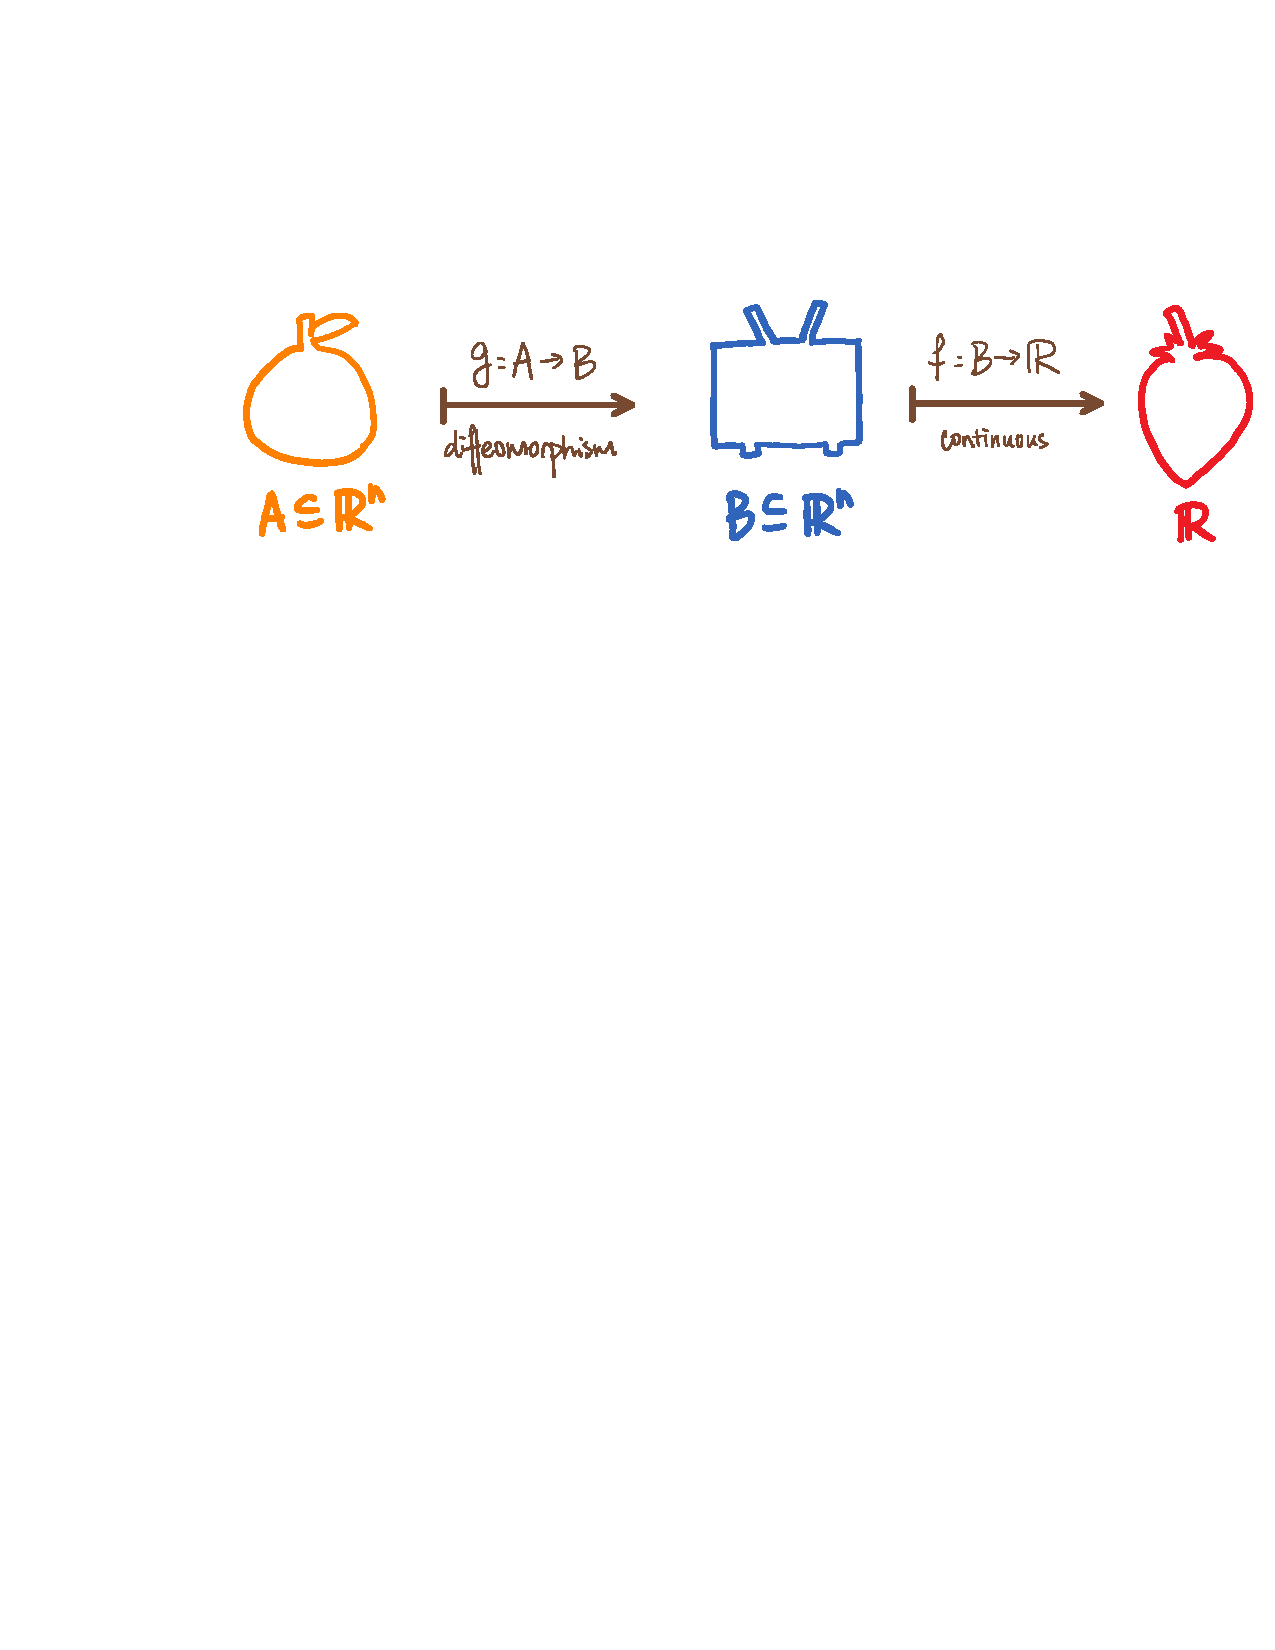
\includegraphics[scale=0.69]{chngOfVar.pdf}
\end{center}

\begin{defn}
Let $Q$ be a box in $\R^n$, and consider an affine map $T:\R^n \to \R^k \ \ \ \vec{x}\mapsto M\vec{x}+\vec{b}$ that maps $Q$ to $P$. $P$ is called a parallelepiped.  
\end{defn}
\note Given the settings in Definition 13.0.0.0.1, $P$ is rectifiable, and we have: $$V(P) = |\det(M)| \cdot V(Q)$$

\hfill\break
\begin{defn}
Let $C$ be a compact rectifiable set in $\R^{n-1}$ for $n \geq 2$, let $\phi:C \to \R$ and $\psi:C \to \R$ be continuous functions such that $\phi(x) \leq \psi(x)$ for all $x \in C$. The set defined by the following is called a simple region in $\R^n$:
$$S\coloneqq \{(x,t) \mid x \in C,\ \phi(x) \leq t \leq \psi(x)\}$$
\end{defn}

\hfill\break
\begin{lem}[Lemma 14.3 on Munkres]
Simple regions are compact and rectifiable.
\end{lem}

\begin{thm}[Fubini's Theorem for Simple Regions]
Let $S\coloneqq \{(x,t) \mid x \in C,\ \phi(x) \leq t \leq \psi(x)\}$ be a simple region in $\R^n$, where $C$ is a compact rectifiable set in $\R^{n-1}$ for $n \geq 2$, $\phi:C \to \R$ and $\psi:C \to \R$ are continuous functions with the property $\phi(x) \leq \psi(x)$ for all $x \in C$, let $f:S \to \R$ be a continuous function. Then $f$ is integrable over $S$ and we have the following holds: 
$$\int_S f = \int_{x \in C} \int_{t=\phi(x)}^{t=\psi(x)} f(x,t)\, dt\, dx$$
\end{thm}
\begin{proof}
The proof of this theorem is given by Theorem 14.4 on Munkres.
\end{proof}
\newpage

\begin{thm}[Substitution Rule]
Let $I = [a,b]\subseteq \R$, let $g:I \to \R$ be a function of $C^1$ type, with $g'(x) \neq 0$ for all $x \in (a,b)$. Then the set $g(I)$ is a closed interval $J$ with end points $g(a)$ and $g(b)$. For continuous function $f:J \to \R$, we have the following holds:
$$\int_{g(a)}^{g(b)} f = \int_a^b (f\circ g) g'\qquad\qquad\qquad \int_J f = \int_I (f\circ g)|g'|$$
\end{thm}
\begin{proof}
The proof of this theorem is given by Theorem 17.1 on Munkres.
\end{proof}


\begin{thm}[Change of Variable Theorem]
Let $A$ be an open subset of $\R^n$, let $B$ be an open subset of $\R^n$, and let $g$ be a diffeomorphism from $A$ to $B$. For continuous function $f:B\to \R$, $f$ is integrable over $B$ if and only if the function $(f\circ g) \cdot |\det Dg|$ is integrable over $A$. Moreover, if $f$ is integrable over $B$, we have the following holds:
$$ext \int_B f = ext \int_A (f\circ g) \cdot |\det Dg|$$ 
That is, for continuous function $f:B \to \R$, either $ext \int_B f = ext \int_A (f\circ g) \cdot |\det Dg|$, or neither $ext \int_B f$ nor $ext \int_A (f\circ g) \cdot |\det Dg|$ exists.
\end{thm}

\note (The restriction of the Change of Variable Theorem on $\R$)\\
First we generalize the the Substitution Rule as a consequence of the Change of Variable Theorem:
Given the settings in Theorem 13.3, suppose we have $n=1$, and suppose further $A\subseteq \R$ is an open connected set, that is, we can write $A= (\alpha,\beta)$. In such case, the diffeomorphism $g$ defined on $A$ must be strictly monotonic, and we have either (1) $B = (g(\alpha),g(\beta))$,  or (2) $B = (g(\beta),g(\alpha))$. For case (1), we can write: $$ext \int_{(g(\alpha),g(\beta))} f = ext \int_{(\alpha,\beta)} (f\circ g)\cdot g'$$ 
For case (2), we have: 
$$ext \int_{(g(\beta),g(\alpha))} f = -ext\int_{g(\alpha)}^{g(\beta)} f=- ext \int_{(\alpha,\beta)} (f\circ g)\cdot g' $$
These results follows immediately from the Substitution Rule, one can use Chain Rule and Fundamental Theorem of Calculus to prove these results easily.\\



\begin{proof}[Proof of Theorem 13.3]
\hfill\break
We start with some temporary added assumptions:
\begin{enumerate}[topsep=3pt,itemsep=-1ex,partopsep=1ex,parsep=1ex]
\item $f \in C(\bar{B},\R)$
\item $A,B$ are bounded and rectifiable
\item $g$ is a diffeomorphism from an open set containing $\bar{A}$ to an open set containing $\bar{B}$
\end{enumerate}

First we consider Special Case 1: \\
Suppose the function $g$ defined in the settings of Theorem 13.3 is a coordinate transposition that maps $(x_1,\cdots, x_l,\cdots,x_k,\cdots,x_n)$ to $(x_1,\cdots x_k, \cdots, x_l, \cdots, x_n)$. Then we know that $\det (Dg(\vec{x})) = -1 \Rightarrow |\det (Dg(\vec{x}))| =1$ for all $\vec{x}\in A$. Note that reorienting boxes does not alter their volume, then we can write:
$$\int_B f = \int_A f\circ g = \int_A (f\circ g)|\det(Dg)|$$ use extended integral when appropriate. This completes the proof of Theorem 13.3 for this Special Case 1. In this rest of the proof of Theorem 13.3, we will call such coordinate transposition function $g$ as Type-1 diffeomorphism.\\


Now consider Special Case 2: \\
Suppose the set $B$ defined in the settings of Theorem 13.3 is given by the following: 
$$B = \left\{ \vec{x}=(x_1,x_2,\cdots,x_n)\in \R^n\left|\ \substack{(x_1,\cdots, x_{n-1}) \in E,\\ \phi(x_1,\cdots, x_{n-1}) < x_n < \psi(x_1,\cdots, x_{n-1})}\right.\right\}$$
where $E$ is a bounded open rectifiable subset of $\R^{n-1}$, $\phi,\psi \in C(\bar{E}, \R)$ with $\phi(\vec{x}) < \psi(\vec{x}) $ for all $\vec{x}\in E$. Suppose further that the function $g$ defined in the settings of Theorem 13.3 maps $(x_1,x_2,\cdots, x_{n-1}, x_n)$ to $(x_1,\cdots, x_{n-1}, \alpha(\vec{x}))$, for some function $\alpha:A \to \R$. Here we can write: 
$$A = \{ \vec{x}\mid (x_1,\cdots,x_{n-1}) \in E , \phi(x_1,\cdots, x_{n-1}) < \alpha(\vec{x}) < \psi(x_1,\cdots,x_{n-1})\}$$
And we see that we get the followings:
\begin{enumerate}[topsep=3pt,itemsep=-1ex,partopsep=1ex,parsep=1ex]
\item $A$, $B$ are rectifiable by Lemma 14.3 on Munkres.
\item Given $\vec{x}' = (x_1,x_2,\cdots, x_{n-1}) \in E$, we see that: $$\vec{x}=(\vec{x}',x_n) \in A \iff x_n \text{ belongs to an interval determined by } \vec{x}'$$
\item Given $\vec{x}\in A$, we have $\det(Dg(\vec{x})) = D_n\alpha(\vec{x})$ because we have:
$$Dg(\vec{x})= \bmat{1&0&\cdots&0 \\ 0 & 1 & \cdots & 0 \\ \vdots &\vdots & &\vdots \\ D_1\alpha(\vec{x})& D_2\alpha(\vec{x}) &\cdots &D_n \alpha(\vec{x})}$$
\end{enumerate}

Let $\vec{x}' = (x_1,x_2,\cdots,x_{n-1})$ denote a vector in $E$, let $\vec{x} = (\vec{x}',x_n)$ denote a vector in $A$ determined by $\vec{x}'$, and let $I_{\vec{x}'}\subseteq \R$ denote the interval determined by $\vec{x}'$. By Fubini's Theorem on Simple Regions and Substitution Rule, one can write the following:
\begin{align*}
\int_B f &= \int_{\vec{x}' \in E} \int_{x_n \in (\phi(\vec{x}'), \psi(\vec{x}'))} f \\
&= \int_{\vec{x}' \in E} \int_{\alpha(\vec{x}) \in I_{\vec{x}'}} (f\circ g) |D_n\alpha| \\
&= \int_A (f\circ g) |D_n\alpha| = \int_A (f\circ g) |\det Dg|
\end{align*}
This completes the proof of Theorem 13.3 for Special Case 2. In the rest of the proof of Theorem 13.3, we will call the function $g$ defined in Special Case 2 as Type-2 diffeomorphism. \\


\newpage
To proceed, we will make use of the following proposition:
\begin{prop}
\setlength{\leftskip}{1cm}Let $A,B,C$ be open subsets of $\R^n$, let $g:A \to B$ and $h:B \to C$ be diffeomorphisms, and let $f:C \to \R$ be a continuous function. If $f$ is integrable over $C$, and $f\circ h$ is integrable over $B$, then we have $\int_C f =\int_A (f\circ (h \circ g))| \det(D(h\circ g))|$. 
\end{prop}
\begin{proof}\setlength{\leftskip}{1cm}By the Change of Variable Theorem, one can write the following:
\begin{align*}
\qquad\qquad\int_C f = \int_B (f\circ h) |\det(D h)| &= \int_A ((f\circ h) \circ g) |\det (Dh)| \cdot g |\det(Dg)| \\
&= \int_A f\circ h \circ g |\det (D(h\circ g))|
\end{align*}
Use extended integral here when appropriate.
\end{proof}

Now suppose the function $g$ defined in the settings of Theorem 13.3 can be characterized by the following: $$g:A \to B \qquad\vec{x} =(x_1,\cdots,x_{j-1},x_j,x_{j+1},\cdots, x_n) \mapsto (x_1,\cdots, x_{j-1}, \eta(\vec{x}), x_{j+1},\cdots, x_n)$$
for some function $\eta:A \to \R$. Such diffeomorphism is called a generalized shear. In the rest of the proof of Theorem 13.3, we will call generalized shear as Type-3 diffeomorphism. Notice that, Type-3 diffeomorphisms can be obtained by compositions of of Type-1 and Type-2 diffeomorphism. Combing Proposition 13.3.1 with Special Case 1 and Special Case 2, it follows that the results of Theorem 13.3 holds for Type-3 diffeomorphism. Note that Type-1 diffeomorphism is a composition of two Type-3 diffeomorphism. Check Page 157 on Munkres for details.\\

The following proposition and theorem ensure that one can locally factorize any diffeomorphism into compositions of Type-1 and Type-2 diffeomorphism.

\begin{prop}\setlength{\leftskip}{1cm}
Any invertible affine map can be factored into composition of affine maps of Type-1 and Type-2, or equivalently, composition of Type-1 and Type-3.
\end{prop}
\begin{proof}\setlength{\leftskip}{1cm}
For linear maps, this follows from element matrix factorization from Theorem 2.4 on Munkres. For translation maps, one can move one coordinate at a time by using Type-3 diffeomorphism. All invertible affine maps can be obtained from composition of linear maps and translation maps. This completes the argument of this proposition.
\end{proof}

\begin{thm}[Theorem 18.3 on Munkres]\setlength{\leftskip}{1cm}
Let $A,B$ be open subset of $\R^n$, let $g:A \to B$ be a diffeomorphism, let $\vec{p}\in A$ with $g(\vec{p}) = \vec{q}\in B$. In some neighborhood of $\vec{p}$, the diffeomorphism $g$ can be factored into a composition of Type-1 diffeomorphisms and Type-2 diffeomorphisms. 
\end{thm}
\begin{proof}\setlength{\leftskip}{1cm}
Let $C$ denote the matrix $Dg(\vec{p})$. Since $g$ is a diffeomorphism, then by the Inverse Function Theorem, we know that $C$ is invertible. Define the following invertible affine maps:
$$\ \ \ \qquad t_1:\R^n \to \R^n\ \ \ \vec{x}\mapsto\vec{x}+\vec{p} \quad\qquad t_2:\R^n \to \R^n \ \ \ \vec{x}-\vec{q}\quad\qquad t_3:\R^n \to \R^n \ \ \ \vec{x}\mapsto C^{-1}\vec{x}$$
\newpage
Now let $T_1=t_2^{-1}\circ t_3^{-1}$ and $T_2=t_1^{-1}$, we get the followings:
\begin{enumerate}[topsep=3pt,itemsep=-1ex,partopsep=1ex,parsep=1ex,leftmargin=2cm]
\item $\hat{g} \coloneqq T_1^{-1} \circ g \circ T_2^{-1}$ is a diffeomorphism, $g = T_1 \circ \hat{g} \circ T_2$.
\item $T_2(\vec{p}) = \vec{0}$, and $T_1(\vec{0}) = \vec{q}$
\item $D\hat{g}(\vec{0}) = I $, where $I$ is the $n \times n$ identity matrix.
\end{enumerate}
From (2), we get $\hat{g}(\vec{0}) = \vec{0}$. \\
From (3), we get $D\hat{g}_k(\vec{0}) = \vec{e}_k^T$.\\
From Chain Rule, we get $DT_1= Dg(\vec{p})$ and $DT_2 = I$. \\ 
Now we define the following maps:
\begin{align*}
\quad\qquad
\bmat{x_1\\x_2\\x_3\\\cdots,\\x_n} \mapsto \bmat{\hat{g}_1(\vec{x})\\x_2\\x_3\\\cdots \\x_n} \quad\qquad
\bmat{x_1\\x_2\\x_3\\\cdots,\\x_n}\mapsto \bmat{\hat{g}_1(\vec{x})\\\hat{g}_2(\vec{x})\\x_3\\\cdots\\ x_n} \quad\qquad
\cdots \qquad\quad
\bmat{x_1\\x_2\\x_3\\\cdots,\\x_n} \mapsto \hat{g}(\vec{x})
\end{align*}
By the Inverse Function Theorem, each of these maps is a diffeomorphism in some neighborhood of $\vec{0}$ because the derivative of each of them at $\vec{0}$ is $I$. We observe that each of these maps is a Type-3 diffeomorphism. Then we get an induced map given by the following:
$$\qquad\qquad\bmat{x_1\\x_2\\x_3\\\cdots,\\x_n} \mapsto \bmat{\hat{g}_1(\vec{x})\\x_2\\x_3\\\cdots \\x_n} \mapsto \bmat{\hat{g}_1(\vec{x})\\\hat{g}_2(\vec{x})\\x_3\\\cdots\\ x_n} \mapsto
\cdots \mapsto \hat{g}(\vec{x})$$
Combining with Proposition 13.3.2, the result follows.
\end{proof}

Concluding the above, we have got a local version of Theorem 13.3. To finish the proof of Theorem 13.3, we will need the Partition of Unity Theorem to partition the function $f$ on the open set $B$.

\begin{defn}
Let $X$ be a metric space, and let $V$ be a vector space, let $f:X \to V$.
The support of $f$, denoted as $supp(f)$, is defined to be the closure of the set $\{\vec{x}\mid f(\vec{x}) \neq \vec{0}\}$ in $X$.
\end{defn}

\note Let $X$ be a metric space, and let $V$ be a vector space, let $f:X \to V$. \\For $\vec{x}\in X$, $\vec{x}\notin supp(f)$ if and only if $\exists\ \epsilon > 0$ such that $f(\vec{t}) = \vec{0}$, $\forall \vec{t}\in B_\epsilon(\vec{x})$. 

\begin{corT}\setlength{\leftskip}{1cm}
Let $A,B$ be open subset of $\R^n$, let $g:A \to B$ be a diffeomorphism, let $\vec{p}\in A$ with $g(\vec{p}) = \vec{q}\in B$. There exists some open neighborhood $U$ of $\vec{p}$, and some open neighborhood $V$ of $\vec{q}$ such that $g|_U:U \to V$ defines a diffeomorphism that can be factored into Type-1 and Type-2 diffeomorphisms. For some continuous function $f:B \to \R$, if $supp(f) \subseteq U$, then we have either $ext \int_B f = ext \int_A (f\circ g) \cdot |\det Dg|$, or neither $ext \int_B f$ nor $ext \int_A (f\circ g) \cdot |\det Dg|$ exists.
\end{corT}

\begin{center}
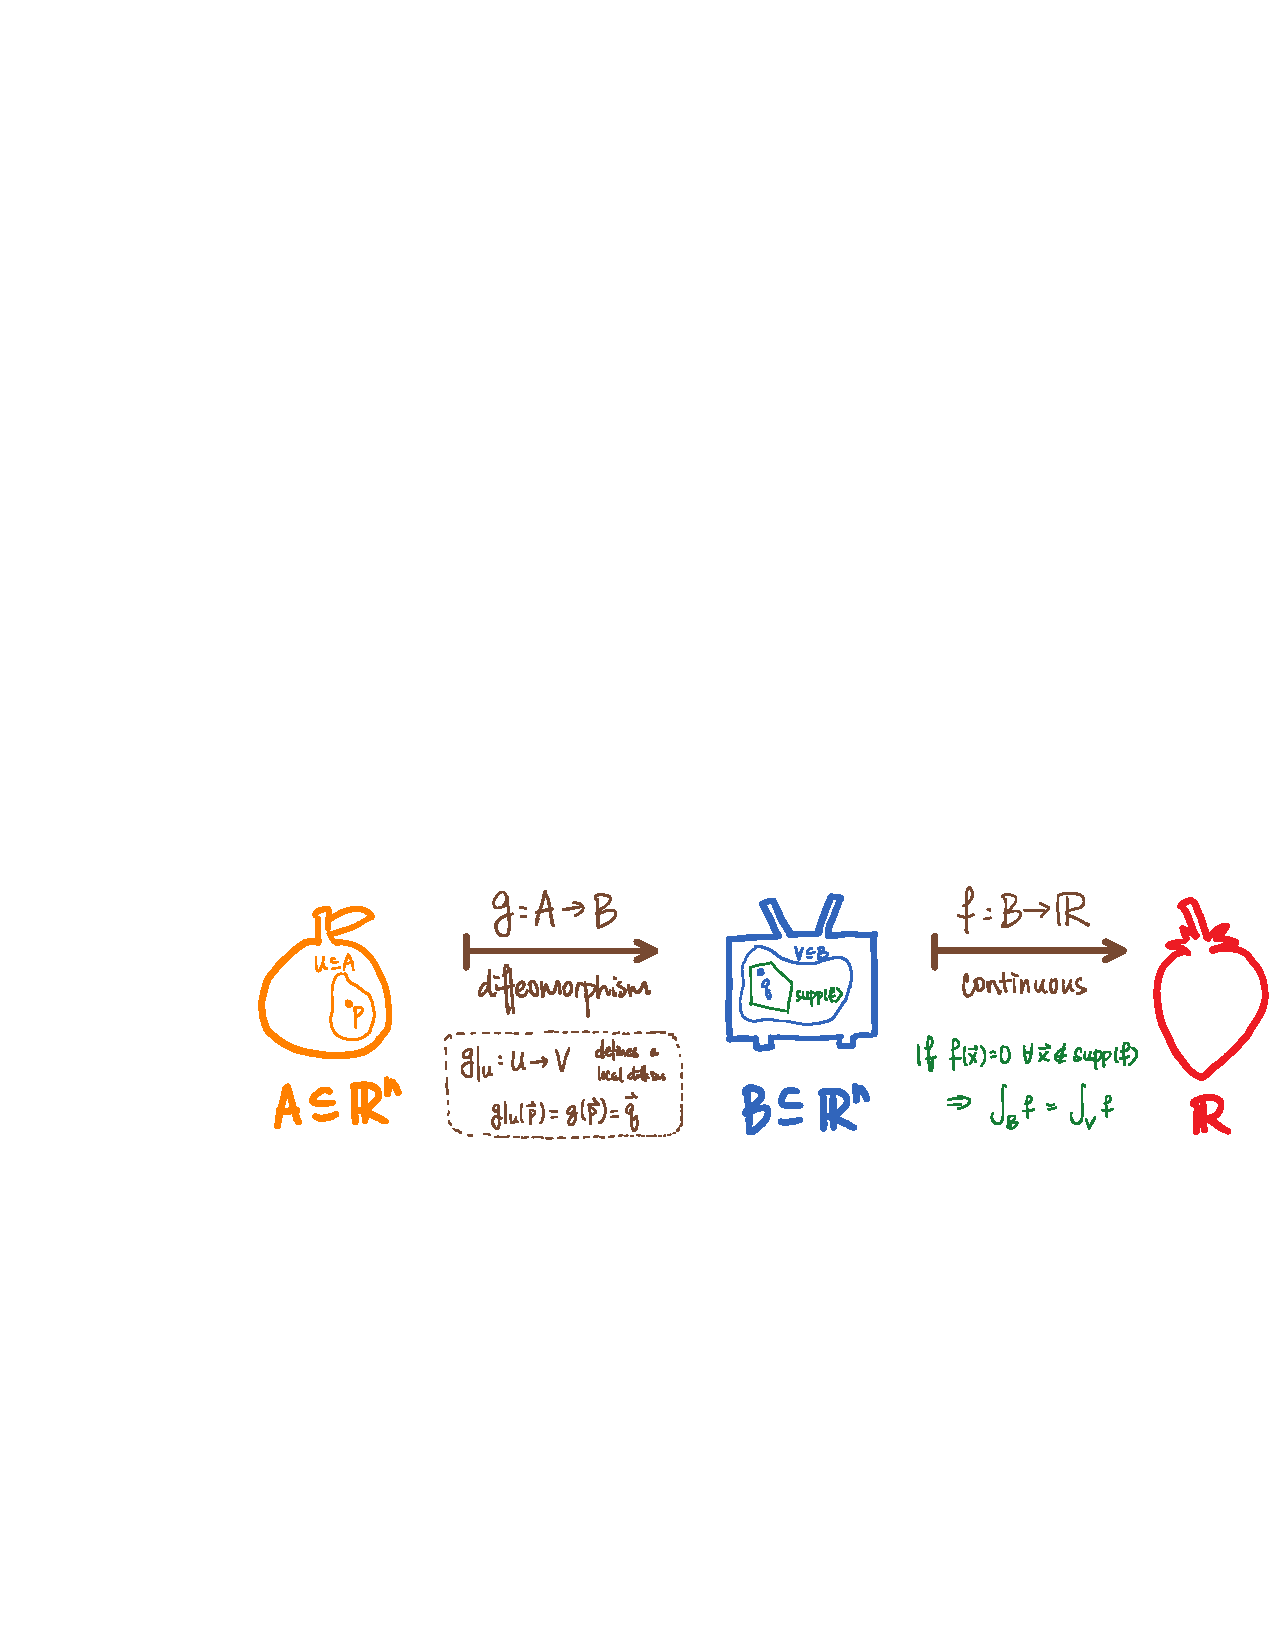
\includegraphics[scale=0.69]{cor13.4.pdf}
\end{center}

The Partition of Unity Theorem gives us a way to partition the function $f$ on the open set $B$ such that the support of each partition of $f$ is contained in some desired open subset of $B$, in which case we can apply Corollary 13.4.1 to complete the proof of the Change of Variable Theorem.

\begin{lem}
\setlength{\leftskip}{1cm}The function $f$ given by the following belongs to $C^\infty (\R,[0,\infty))$: $$f:\R \to \R \ \ \ \begin{cases}e^{-1/x} &x>0\\0&x\leq 0  \end{cases}$$
\end{lem}
\begin{proof}
\setlength{\leftskip}{1cm}The proof of this lemma is given in Spivak Chapter 18.
\end{proof}

\begin{corL}
\setlength{\leftskip}{1cm}Consider the function: 
$$f:\R \to \R \ \ \ \begin{cases}e^{-1/x} &x>0\\0&x\leq 0  \end{cases}$$
For the box $Q = [a_1,b_1]\times [a_2,b_2] \times \cdots \times [a_n,b_n]$, the function characterized by $\Phi_Q(\vec{x}) = f(x_1-a_1)f(b_1-x_1)\cdots f(x_n-a_n)$ is in $C^\infty(\R^n,[0,\infty))$, with they property that $supp(\Phi_Q) = Q$ and $\Phi_Q (\vec{x})> 0$ for all $\vec{x}\in Q$. 
\end{corL}


\begin{lem}
\setlength{\leftskip}{1cm}One can find positive volume boxes $Q_1,Q_2,\cdots$ such that the following holds:
\begin{enumerate}[topsep=3pt,itemsep=-1ex,partopsep=1ex,parsep=1ex,leftmargin=1.5cm]
\item $\Omega = \bigcup_j \Int(Q_j)$
\item Each $Q_j$ is contained in some $U_{\alpha_j}$
\item Each $y \in \Omega$ has neighborhood meeting only finitely many $Q_j$,\\ such property is called the local finiteness 
\end{enumerate} 
\end{lem}
\begin{proof}
\setlength{\leftskip}{1cm}Write $\Omega = K_1 \cup K_2\cup \cdots$ with each $K_j$ being compact, and $K_j \subseteq \Int(K_{j+1})$. Check Lemma 15.1, or a previous theorem in this text. Let $E_j = K_j \setminus \Int(K_{j-1})$, each $E_j$ is compact, and disjoint from $K_{j-2}$ for $j \geq 3$. Here we have:
$$E_j \subseteq \Int(\hat{Q}_{j,1}) \cup \cdots \cup \Int(\hat{Q}_{j,M_j})$$ 
with each $\hat{Q}_{j,k}$ contained in some $U_\alpha$, and each $\hat{Q}_{j,k}$ is disjoint from $K_{j-2}$. Then we can write $\Omega = \bigcup_{j,k} \Int(\hat{Q}_{j,k})$. $K_j$ meets at most $M_{i} + \cdots + M_j$ of the $\hat{Q}_{j,k}$. Relabel the $\hat{Q}_{j,k}$ as $Q_1,Q_2,Q_3,\cdots$ This completes the proof of the lemma. 
\end{proof}

Now we have got our setup for the Partition of Unity Theorem.

\newpage
\begin{thm}[Partition of Unity Theorem]
\setlength{\leftskip}{1cm}Let $\Omega$ be an open subset of $\R^n$. If $\Omega = \bigcup_{\alpha \in A} U_\alpha$ for some open subsets $U_\alpha$ of $\R^n$, then there exist some functions $\phi_1,\phi_2,\cdots \in C^\infty(\Omega, [0,\infty))$ such that we have:
\begin{enumerate}[topsep=3pt,itemsep=-1ex,partopsep=1ex,parsep=1ex,leftmargin=1.5cm]
\item Each $supp(\phi_j)$ is compact
\item Each $supp(\phi_j)$ is contained in some $U_\alpha$
\item Each $\vec{x}\in \Omega$  has an open neighborhood that intersects only finitely many $supp(\phi_j)$
\item $\sum_{j=1}^\infty \phi_j(\vec{x}) = 1$ for all $\vec{x}\in \Omega$, such sum is called the locally finite sum
\end{enumerate}
\end{thm}
\begin{proof}\setlength{\leftskip}{1cm}
The proof of this theorem follows from the Fundamental Theorem of Laziness. Section 16 on Munkres gives a proof for this theorem. Alternatively, consider the following:
Let $\Phi(Q_i)$ be functions defined appropriately similar to those given in Corollary 13.4.2.1. Let $\lambda$ be a function defined by $\lambda(\vec{x}) = \sum_{j=1}^\infty \Phi_{Q_j}(\vec{x})$. Here we have $\lambda \in C^\infty(\Omega,(0,\infty))$, and the following holds: $$1 = \sum_{j=1}^\infty \frac{\Phi_{Q_j}(\vec{x})}{\lambda(\vec{x})} $$ 
Here we let $\phi_j$ be a function characterized by the following: 
$$\phi_j(\vec{x}) \coloneqq \frac{\Phi_{Q_j}(\vec{x})}{\lambda(\vec{x})}$$ 
which is a $C^\infty$ function, and we have $supp(\phi_j) =Q_j$. \\
Then the results of Theorem 13.5 follow immediately. 
\end{proof}

\begin{lem}\setlength{\leftskip}{1cm}
Let $B$ be an open subset of $\R^n$, let $f \in C(B ,\R)$ such that $ext\int_B f$ exists, let $(\phi_j)$ be a sequence of functions in $C^\infty(B,[0,\infty])$ that satisfies conditions (1),(3),(4) in the Partition of Unity Theorem. Then we can write $ext\int_B f = \sum_{j =1}^\infty \int_B \phi_j \cdot f$.
\end{lem}
\begin{proof}\setlength{\leftskip}{1cm}
First we will tackle the case where $f\geq 0$, then apply to $f_+$ and $f_-$ and combine the results. Assume that $f \geq 0$, suppose $E$ is a compact rectifiable subset of $B$. Then there exists $M$ such that $\phi_j = 0$ on $E$ for $j \geq M$. Since $f \geq 0$, here we have the following:
$${}\qquad\int_E f = \int_E \sum_{j=1}^\infty \phi_j\cdot f = \int_E \sum_{j=1}^M \phi_j \cdot f = \sum_{j=1}^M \int_E \phi_j \cdot f  \leq \sum_{j=1}^M \int_B \phi_j \cdot f \leq \sum_{j=1}^\infty \int_B \phi_j \cdot f$$
Take the supremum over $E$, and get the following:
$$ext \int_B f \leq \sum_{j=1}^\infty \int_B \phi_j \cdot f$$
On the other hand, we have the following:
$$\sum_{j=1}^\infty \int_B \phi_j\cdot f = \lim_{M \to \infty} \sum_{j=1}^M \int_B \phi_j\cdot f = \lim_{M\to \infty} \int_B \sum_{j=1}^M \phi_j f \leq ext\int_B f$$
Combine the two inequalities and apply to $f_+$ and $f_-$ to get the result for this Lemma.
\end{proof}

Here we combine the results from above to complete the proof of Theorem 13.3:\\

For $\vec{y}\in B$, choose an open subset $U_{\vec{y}}$ of $B$ such that $g$ can be factorized into Type-1 and Type-2 diffeomorphisms on $U_{\vec{y}}$, then choose a partition of unity $(\phi_j)$ dominated by $\{U_{\vec{y}} \mid \vec{y}\in B \}$. Now we can write the following:
$$ext\int_B f_+ = \sum_{j=1}^\infty \int_A (\phi_j \circ g) (f_+\circ g) |\det Dg| = ext \int_A (f_+\circ g)|\det Dg| $$
$$ext\int_B f_- = \sum_{j=1}^\infty \int_A (\phi_j \circ g) (f_-\circ g) |\det Dg| = ext \int_A (f_-\circ g)|\det Dg| $$
Combining the results for $f_+$ and $f_-$ to get the desired results for Theorem 13.3.
\end{proof}


\note In the settings of Theorem 13.3, suppose we have $g :A \to B \ \ \  \vec{x}\mapsto r \vec{x}$ for some $r >0$, then we can write the following:
$$ext \int_{\vec{x}\in B} f(\vec{x}) = ext\int_{\vec{x}\in A} f(r\vec{x})\cdot r^n$$

\hfill\break
\begin{defn}
The number $\pi$ is defined to be the following:
$$\pi \coloneqq \lambda_2 \coloneqq V(B_1^2(\vec{0}))$$
\end{defn}

\hfill\break

\example Let $B_r^n(\vec{0}) \coloneqq \{ \vec{x}\in \R^n \mid ||\vec{x}|| <r\}$, we have $V(B_r^n(\vec{0})) = r^n V(B_1^n(\vec{0})) \coloneqq r^n\lambda_n$.\\

\newpage
\example We have $\frac{V(B_1^n(\vec{0}))}{V([-1,1]^n)} \leq 1$.
\begin{align*}
\lambda_n = \int_{B_1^n(\vec{0}))} 1 = \int_{\vec{x}\in B_1^k (\vec{0})} \int_{\vec{y}\in B_{\sqrt{1-||\vec{x}||^2}}^{n-k}} 1 = \int_{\vec{x}\in B_1^k(\vec{0})} \left(1-||\vec{x}||^2\right)^{\frac{n-k}{2}} \lambda_{n-k} 
\end{align*}
Here we choose $k=2$, then we can rewrite:
\begin{align*}
\lambda_n &= \lambda_{n-2} \int_{B_1^2(\vec{0})} (1-||\vec{x}||^2)^{\frac{n}{2}-1} \\&= \lambda_{n-2} \int_{B_1^2(\vec{0})\setminus ((-1,0]\times \{0\})} (1-||\vec{x}||^2)^{\frac{n}{2}-1} + \lambda_{n-2} \int_{(-1,0]\times \{0\}} ( 1-||\vec{x}||^2)^{\frac{n}{2}-1}
\end{align*}
Here $\lambda_{n-2} \int_{(-1,0]\times \{0\}} ( 1-||\vec{x}||^2)^{\frac{n}{2}-1} = 0$ by Theorem 11.13 from Munkres. \\
Let $g:\R^2 \to \R^2 \ \ \ (r,\Phi) \mapsto (r\cos(\Phi),r\sin(\Phi))$. Notice that $g$ is a local diffeomorphism and $\det Dg(r,\Phi) = r$. Here we can write the following:
\begin{align*}
\lambda_n &=  \lambda_{n-2} \int_{B_1^2(\vec{0})\setminus ((-1,0]\times \{0\})} (1-||\vec{x}||^2)^{\frac{n}{2}-1} \\
&= \lambda_{n-2} \int_{\{r \mid 0<r<1\}\times \{\Phi \mid -\pi<\Phi <\pi\}} (1-r^2)^{\frac{n}{2}-1} r\\
&= \lambda_{n-2} \int_0^1 \int_{-\pi}^\pi (1-r^2)^{\frac{n}{2}-1} r\, d\Phi\, dr\\
&= 2 \pi \lambda_{n-2} \int_0^1 (1-r^2)^{\frac{n}{2}-1} r\, dr\\
&= \pi \lambda_{n-2} \int_{0}^1 t^{\frac{n}{2}-1}\, dt \\
&= \frac{2\pi\lambda_{n-2}}{n}
\end{align*}
with $t =1-r^2$ and $dt = 2r\, dr$. It follows that, for $u \in \N$, we have: $$\lambda_{2u} = \frac{\pi^u}{u!} \qquad\qquad\qquad\lambda_{2u+1} = \frac{2^{u+1}\pi^u}{(2u+1)(2u-1)(2u-3)\cdots(3)(1)}$$

\exercise
For $n \in \N$, let $\mu_n = V([-1,1]^n) = 2^n$, and let $\kappa_n$ be defined as:
$$\kappa_n = V\left(\left\{\vec{x}=(x_1,x_2,\cdots,x_n)\in \R^n \left|\  \sum_{i=1}^n|x_i| < 1 \right.\right\} \right)= \frac{2^n}{n!}$$
We get $\kappa_n \leq \lambda_n \leq \mu_n$, $\lim_{n\to \infty} \frac{\lambda_n}{\mu_n} = 0$, and $\lim_{n \to \infty} \frac{\kappa_n}{\lambda_n}= 0$. \\

\exercise Let $\Omega$ be a rectifiable subset of $\R^n$, let $h$ be an isometry that maps $\Omega$ to $h(\Omega)$, we have the following holds: $$V(h(\Omega)) = \int_{h(\Omega)} 1 = \int_{\Omega} 1\cdot |\det Dh| = V(\Omega)$$

\newpage
\begin{defn}
Let $A$ be a rectifiable subset of $\R^n$ with positive volume, let $f:A \to \R$ be an integrable function. The average of $f$ over $A$ is defined to be the following: $${\text{avg}}_A f = \frac{\int_A f}{V(A)}$$
\end{defn}
\note In the setting of Definition 13.5.1.0.2, we have $\inf_A f \leq {\text{avg}}_A f \leq \sup_A f$.\\

\begin{defn}
Let $A$ be a rectifiable subset of $\R^n$, and let $f:A\to \R^n \ \ \ \vec{x} \mapsto (f_1(\vec{x}),f_2(\vec{x}),\cdots, f_n(\vec{x}))$ be an integrable function. $$\int_A f \coloneqq \bmat{\int_A f_1 \\ \int_A f_2 \\ \vdots \\ \int_A f_n}$$
\end{defn}
\note In the settings of Definition 13.5.1.0.3, we have the following holds: 
$$\text{avg}_A f\coloneqq \frac{\int_A f}{V(A)}\in \R^n$$ 
and for a special case where $f:\R^n \to \R^n \ \ \ \vec{x}\mapsto \vec{x}$, $\text{avg}_A f$ is called the centroid of $A$. \\
Here we can write:
$$\text{avg}_A f = \bmat{\text{avg}_A \,f_1 \\ \text{avg}_A \, f_2 \\ \vdots \\ \text{avg}_A \, f_n}$$

\remark The height of the centroid of the upper half of a unit sphere is greater than the height of the centroid of the upper half of a unit ball.\\



\newpage
\section[Volume of Parallelopipeds]{\color{red} Volume of Parallelopipeds \color{black}}

\begin{defn}
Let $Q$ be a box in $\R^k$, and let $T$ be an affine injection from $\R^k$ to $\R^n$ of the form $T(\vec{x}) = A\vec{x}+\vec{b}$ for some matrix $A$ and $\vec{b}\in \R^n$. $T(Q)$ is called a $k$-parallelopiped.
\end{defn}

For $k<n$, let $Q$ be a box in $\R^k$, and let $T$ be an affine injection from $\R^k$ to $\R^n$ of the form $\vec{x}\mapsto A\vec{x}+\vec{b}$ for some matrix $A$ and vector $\vec{b}\in \R^n$. $T(Q)$ is a $k$-parallelopiped. Here we note that the $n$-volume of the $k$-parallelopiped $T(Q)$ is always zero because $T(Q)$ lies in a $k$-dimensional subspace of $\R^n$ which has measure zero. We want to find a way to define the $k$-volume of $T(Q)$, denoted as $V_k(T(Q))$. Here are some expectations for such definition: 
\begin{enumerate}[topsep=3pt,itemsep=-1ex,partopsep=1ex,parsep=1ex]
\item In the case where we have: 
$$A = \bmat{M \\ Z}$$ for some $k\times k$ matrix $M$ and zero matrix $Z$, we should have the following: $$V_k(T(Q))= |\det M|\cdot V(Q)$$
\item For isometry $h:\R^n \to \R^n$, we should have the following: $$V_k(h(T(Q))) = V_k(T(Q))$$
\end{enumerate}


\hfill\break
\begin{thm}[Theorem 21.2 from Munkres] 
For $k\leq n$, let $T:\R^k \to \R^n \ \ \ \vec{x} \mapsto A\vec{x}+\vec{b}$ be an affine injection for some matrix $A$ and $\vec{b}\in \R^n$. One can pick an orthogonal $n \times n$ matrix $B$ such that we have: $$B\cdot A= \bmat{M \\ Z}$$ for some $k\times k$ matrix $M$ and zero matrix $Z$.
\end{thm}
\begin{proof}
First $k$ rows of $B$ forms an orthonormal basis for column space of $A$. Extend such orthonormal basis to an orthonormal basis of $\R^n$ to obtain the remaining rows of $B$ by applying the Gram-Schmidt Process. 
\end{proof}


In the settings of Theorem 14.1, we have $(BA)^T = \bmat{M& Z}$, and $(BA)^T (BA) = M^TM$. Now let $h:\R^n \to \R^n \ \ \ \vec{y}\mapsto B\vec{y}$, note that $h$ is an isometry, and we have the following being satisfied:
\begin{align*}
V_k(T(Q)) = V_k(h(T(Q))) &= |\det(M)|\cdot V(Q) \\&= \sqrt{\det(M^TM)}\cdot V(Q) \\&= \sqrt{\det((BA)^T(BA))}V(Q) \\&= \sqrt{\det(A^TA)}\cdot V(Q)
\end{align*}

\begin{lem}
Let $A$ be an $n \times k$ matrix, we have $\ker(A^TA) = \ker(A)$
\end{lem}
\begin{proof}
It is trivial that we have $\ker(A) \subseteq \ker(A^TA)$. On the other hand, if $A^TA\vec{x}=0$ for some $\vec{x}$, then $||A\vec{x}||^2=\left<A\vec{x}, A\vec{x}\right>= \vec{x}^TA^TA\vec{x} = 0 \Rightarrow A\vec{x} = \vec{0}$. This shows that we have $\ker(A^TA)\subseteq \ker(A)$.
\end{proof}

\begin{corL}
Let $A$ be an $n \times k$ matrix, then we have the following:
$$rank(A^TA) = k-\dim(\ker(A^TA))=k-\dim(\ker(A)) = rank(A)$$
\end{corL}

\begin{corL}
Let $A$ be an $n \times k$ matrix. If $k>n$, then $\det(A^TA) = 0$. 
\end{corL}
\begin{proof}
$k>n$ implies $rank(A) \leq n <k$, which implies $rank(A^TA)<k$, hence we have $\det(A^TA) = 0$. This completes the proof.
\end{proof}

\begin{corL}
Let $A$ be an $n \times k$ matrix. If $k<n$, then $\det(AA^T) = 0$.
\end{corL}

\begin{lem}
Let $A$ be an $n \times k$ matrix. We have $A^TA\geq 0$.
\end{lem}
\begin{proof}
For $\vec{x}$, we have $\vec{x}^TA^TA\vec{x} = \left<A\vec{x},A\vec{x}\right>\geq 0$.
\end{proof}

\begin{corL}
Let $A$ be an $n \times k$ matrix. All eigenvalues of $A^TA$ are greater than or equal to $0$.
\end{corL}

\begin{corL}
Let $A$ be an $n \times k$ matrix, $\det(A^TA) \geq 0$. 
\end{corL}

\begin{defn}
Let $Q$ be a box in $\R^k$, and let $T$ be an affine injection from $\R^k$ to $\R^n$ of the form $\vec{x}\mapsto A\vec{x}+\vec{b}$ for some matrix $A$ and vector $\vec{b}\in \R^n$. We define $V_k(T(Q)) = \sqrt{\det(A^TA)}\cdot V(Q)$. 
\end{defn}

In the following discussion, we will show that the $k$-volume of a parallelopied defined in Definition 14.1.2.2.1 is legitimate. Let $Q_1$ be a box in $\R^k$, and let $T_1$ be an affine injection from $\R^k$ to $\R^n$ of the form $\vec{x}\mapsto A_1\vec{x}$ for some matrix $A_1$.\\

First check independent of choices. Suppose $T_1(Q_1)$ can also be obtained by a composition of affine maps $T_2$ and $C$, $T_1(Q_1) = T_2(C(Q_1))$. Here $C$ is a diffeomorphism. \\
\begin{center}
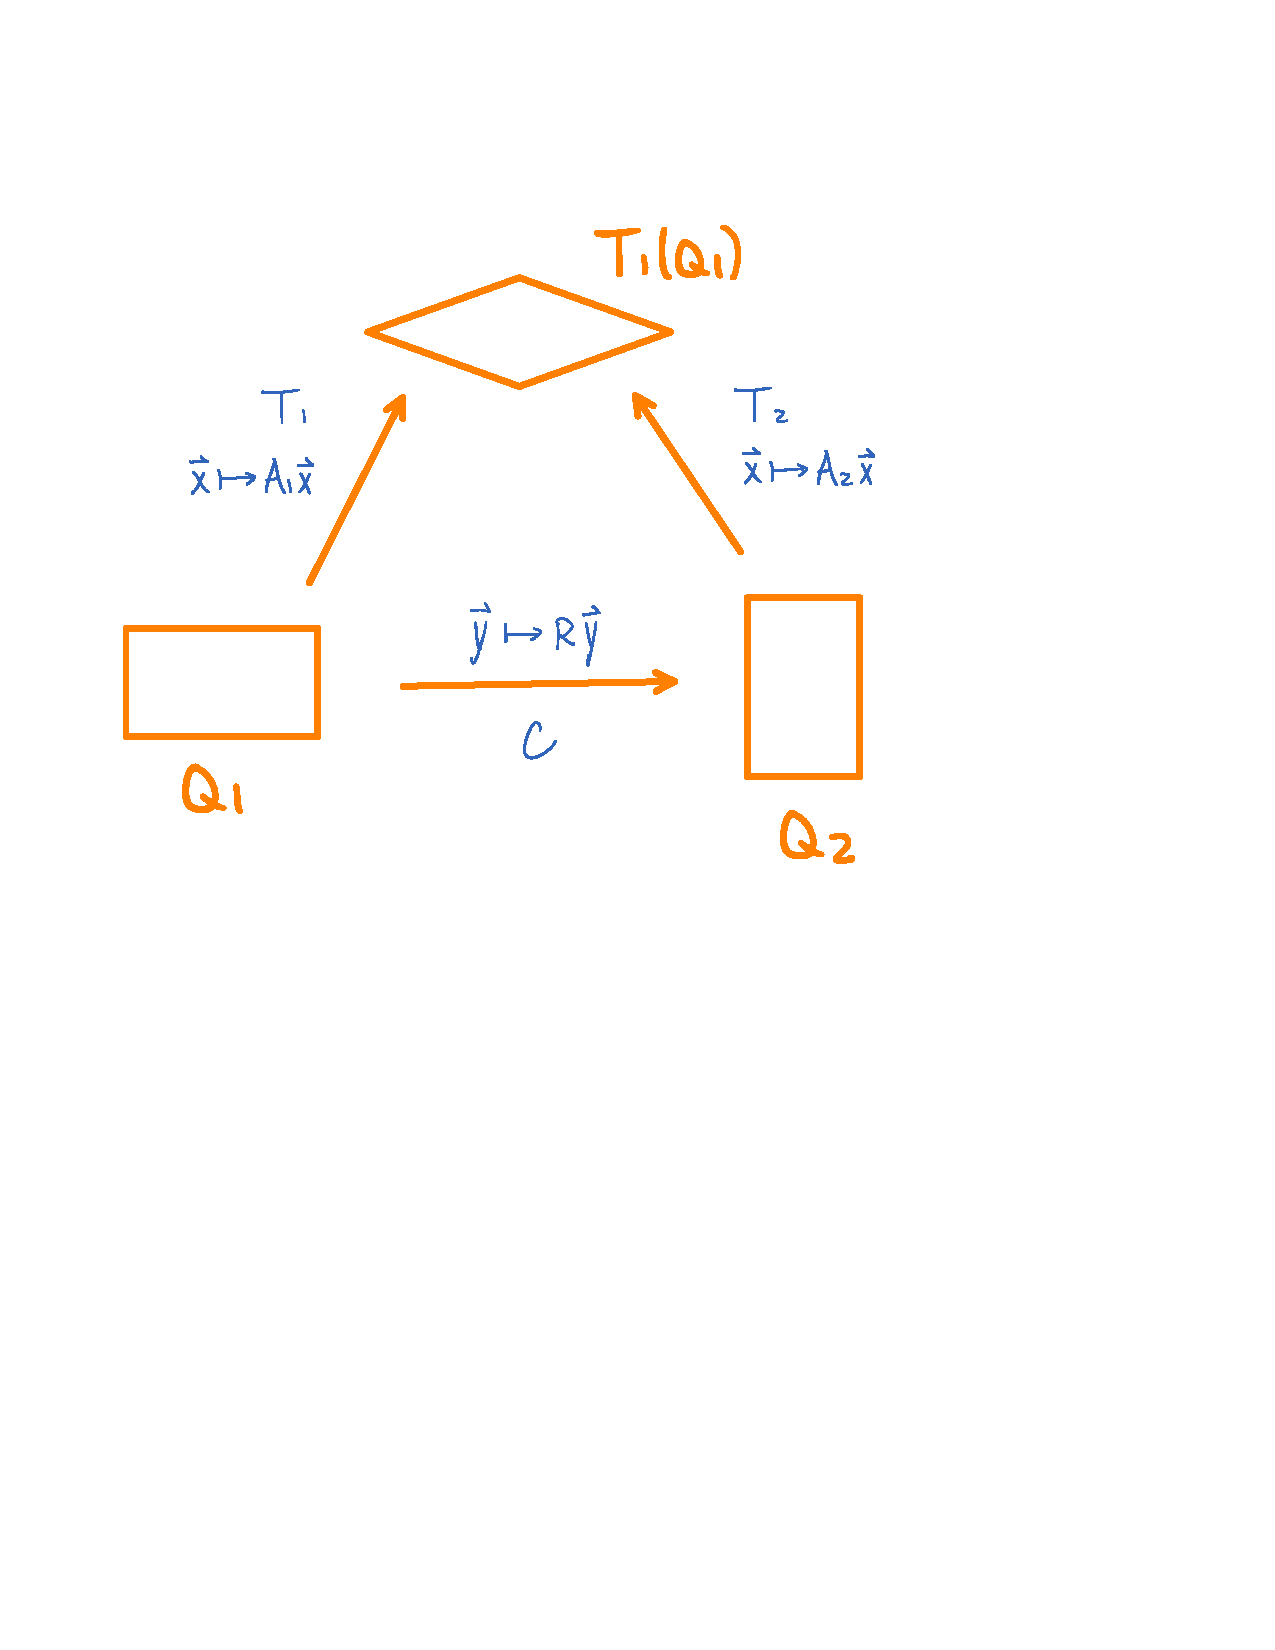
\includegraphics[scale=0.5]{parallpied.pdf}
\end{center}
Let $A_1$ denote the matrix for $T_1$, and let $A_2$ denote the matrix for $T_2$. \\
Here we have $A_1 = A_2 R$, and we can write the following:
\begin{align*}
\sqrt{\det(A_1^TA_1)} \cdot V(Q_1) &= \sqrt{\det((A_2R)^T(A_2R))} \cdot V(Q_1) \\&= \sqrt{\det(R^TA_2^TA_2R)} \cdot V(Q_1) \\&= \sqrt{\det(R^T)\det(A_2^TA_2)\det(R)}\cdot V(Q_1) \\&= \sqrt{\det(A_2^TA_2)}\cdot |\det(R)|\cdot V(Q_1) \\&= \sqrt{\det(A_2^TA_2)}\cdot V(Q_2)
\end{align*}
This shows that the $k$-volume of $T_1(Q_1)$ is well-defined. \\
Now we will check the expectations for the definition of $k$-volume of a parallelopiped:
\begin{enumerate}[topsep=3pt,itemsep=-1ex,partopsep=1ex,parsep=1ex]
\item If $A_1 = \bmat{M \\ Z}$ for some $k\times k$ matrix $M$ and zero matrix $Z$, then we have: 
$$V_k(T_1(Q_1))= |\det M|\cdot V(Q_1)$$
\item For isometry $h:\R^n \to \R^n$, we should have the following:
$$V_k(h(T(Q))) = V_k(T(Q))$$
\end{enumerate}
For expectation (1). Suppose we have $A_1 = \bmat{M&Z}^T$, then we see that we have: 
$$\sqrt{\det(A_1^TA_1)} = \sqrt{\det(M^TM)} = |\det(M)|$$ 
which implies $V_k(T_1(Q_1)) = |\det(M)| V(Q_1)$. For  expectation (2). Consider an isometry defined by $h:\vec{x}\mapsto B\vec{x}+\vec{p}$ for some orthogonal matrix $B$, we see that we have $\det((BA_1)^T(BA_1)) = \det(A_1^TA_1)$, hence it follows that $V_k(h(T_1(Q_1))) = V_k(T_1(Q_1))$.\\

So we see that there exists a map 
$V_k: \{k-\text{parallelopipeds}\}\mapsto (0,\infty)$ that satisfies expectation (1) and expectation (2) that can define the $k$-volume of a parallelopiped, given by the following:
$$V_k(T(Q)) = \sqrt{\det(A^TA)}\cdot V(Q)$$

\begin{defn}
Let $A$ be an $n \times k$ matrix. $\mathcal{V}(A) \coloneqq \sqrt{\det(A^TA)}$
\end{defn}

\begin{thm}[Pythagorean Theorem]
For $n\geq k$, let $A$ be an $n \times k$ matrix. \\
$(\mathcal{V}(A))^2=$ the sum of the squares of the determinant of $k \times k$ sub-matrices of $A$. 
\end{thm}
\begin{proof}
The proof of this theorem is given in Theorem 21.4 on Munkres.
\end{proof}

\begin{corT}
Let $\vec{a}=(a_1,a_2,\cdots,a_n),\vec{b}=(b_1,b_2,\cdots,b_n)\in \R^n$. \\$$\left[\text{the one dimensional volume of the line segment from }\vec{a}\text{ to }\vec{b}\right]^2 = \sum_{j=1}^n (b_j - a_j)^2$$
\end{corT}
\begin{proof}
Proceed by using the affine map $f:[0,1] \to \R^n \ \ \ t\mapsto t(\vec{b}-\vec{a})+\vec{a}$. 
\end{proof}

\newpage
\chapter{Differentiable Manifolds \ \rom{1}}
\setcounter{section}{14}
There are three kinds of non-affine $k$-dimensional objects. 
\begin{enumerate}[topsep=3pt,itemsep=-1ex,partopsep=1ex,parsep=1ex]
\item Parametrized $k$-manifold, discussed in section 22 on Munkres
\item $k$-manifold in $\R^n$, discussed in section 23 on Munkres
\item Abstract $k$-manifold, discussed in section 41 on Munkres
\end{enumerate} 

\section[Parametrized Manifolds]{\color{red} Parametrized Manifolds \color{black}}

\begin{defn}
Let $k,n,r\in \N$ with $k \leq n$, let $\alpha \in C^r(U, \R^n)$, where $U$ is an open subset of $\R^k$.  The set $Y \coloneqq \alpha(U)$, equipped with the map $\alpha$, constitute a parametrized $k$-manifold of class $C^r$, denoted as $Y_\alpha$. The $k$-volume of $Y_\alpha$ is defined by the following:
$$V_k(Y_\alpha) \coloneqq ext \int_U \mathcal{V}(D\alpha)$$
\end{defn}

\remark In the settings of Definition 15.0.0.0.1, for a special case where we have $k=n$, we will have $\mathcal{V}(D\alpha) = |\det D\alpha|$. Suppose further $Y$ is an open rectifiable subset of $\R^n$, and $\alpha:U \to Y$ is a diffeomorphism, then we have: 
$$V_n(Y_\alpha) = \int_U|\det (D\alpha)| = \int_Y 1 = V(Y)$$
In such case, we consider an example where $U = (0,1) \times (0,3\pi)$, and $\alpha$ defined by:
\begin{center}
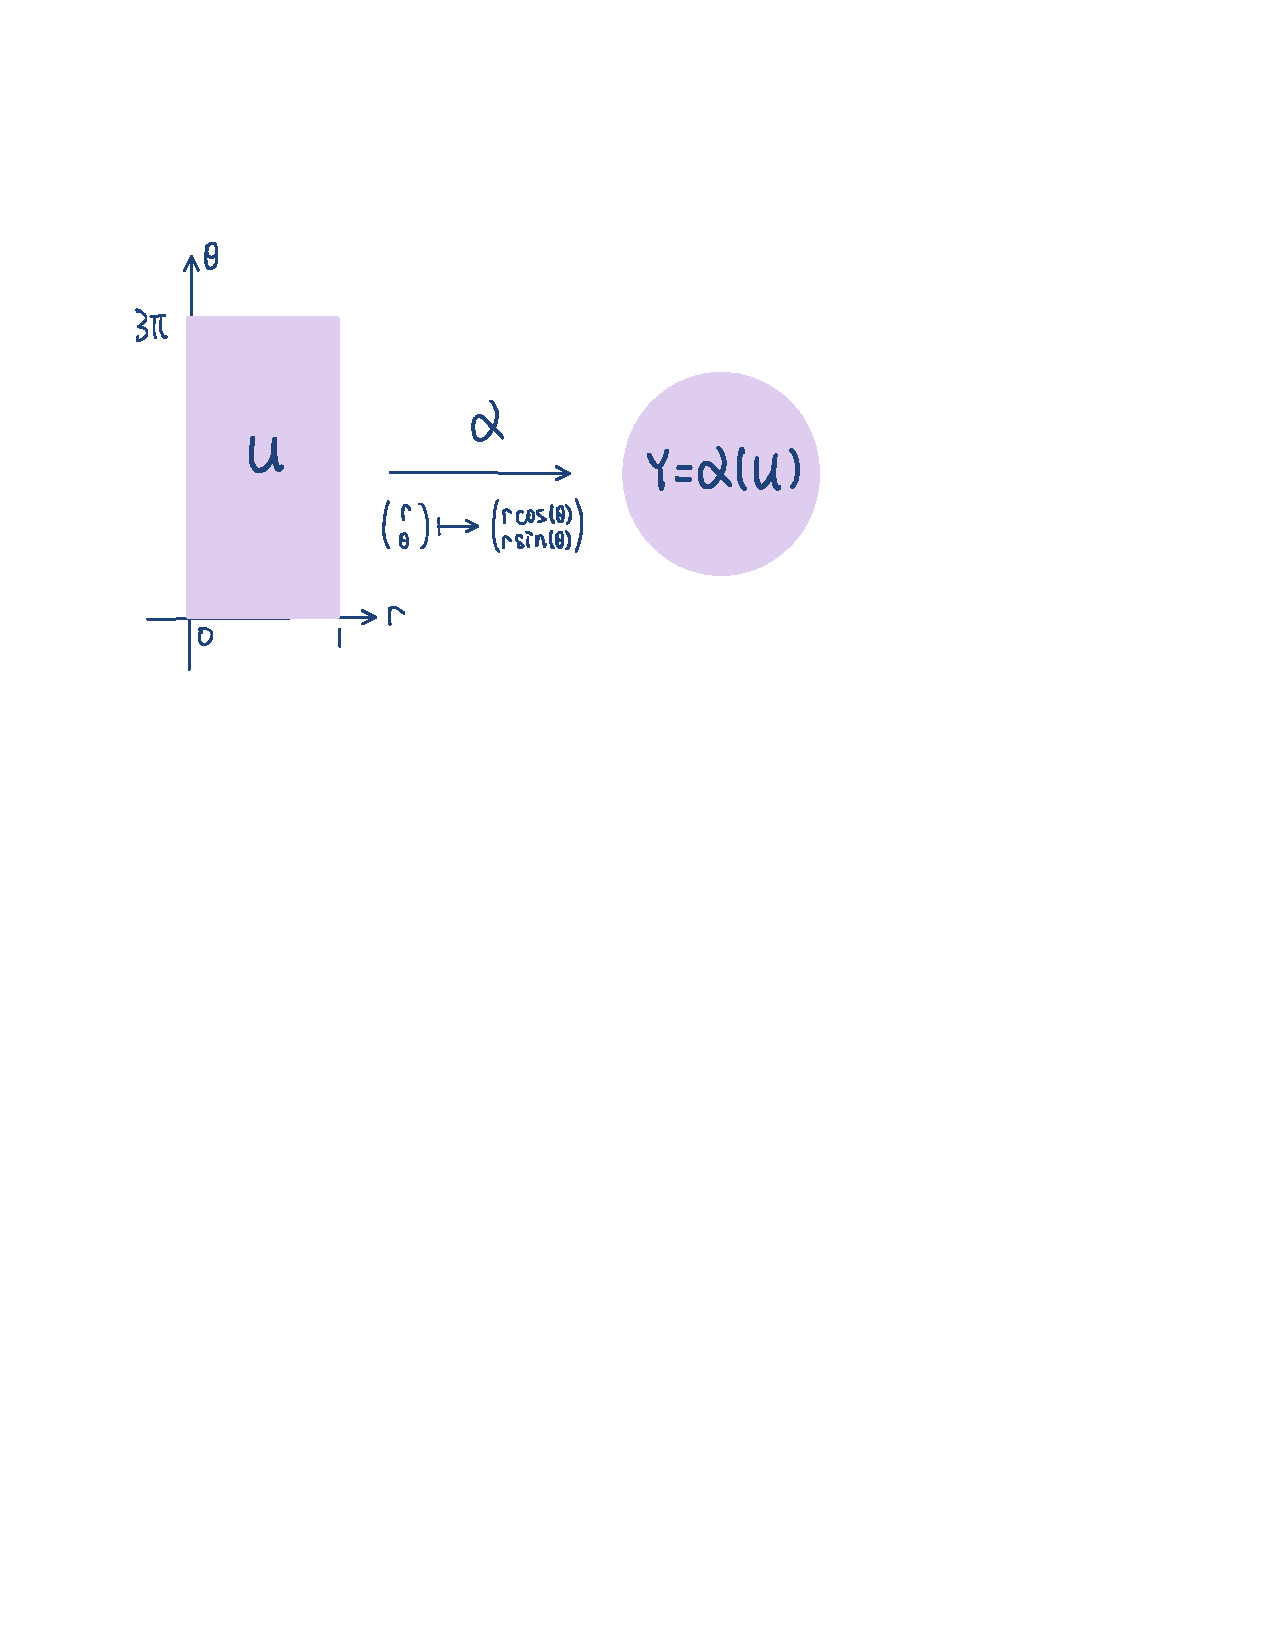
\includegraphics[scale=0.6]{par-manifold.pdf}
\end{center}
Here we have: $V_2(Y_\alpha) = \int_U r = \int_0^1 \int_0^{3\pi} r\, d\Phi \, dr = \frac{3}{2}\pi$.\\

\newpage
\note Let $U$ and $V$ be open sets, $\alpha \in C^r(U,\R^n)$, $\beta\in C^r(V,\R^n)$ with $\alpha(U) = \beta(V)$. \\
If there is a diffeomorphism $g$ from $U$ to $V$, then we can write:
\begin{align*}
V_k(Y_\alpha) &= \int_U \sqrt{\det((D(\beta\circ g))^TD(\beta \circ g))} \\
&= \int_U \sqrt{\det\left((Dg)^T \, \left((D\beta)^T\circ g\right) \, \left(D\beta)\circ g\right)\, Dg\right)}\\
&= \int_U \sqrt{\det(Dg^T) \cdot \det(((D\beta)^T\circ g)(D\beta\circ g))\cdot \det (Dg)}\\
&= \int_U \sqrt{\det(((D\beta)^T\circ g)(D\beta\circ g))} |\det(Dg)|\\
&= \int_V \sqrt{\det((D\beta)^T(D\beta)}= \int_V \mathcal{V}(D\beta)= V_k(Y_\beta)
\end{align*}

\hfill\break
\begin{defn}
Let $Y_\alpha$ be a parametrized $k$-manifold of class $C^r$ with $Y = \alpha(U)$. \\
Given $f \in C(Y,\R)$, we define: $$\int_{Y_\alpha} f\, dV \coloneqq ext \int_U (f\circ \alpha) \mathcal{V}(D\alpha)$$
\end{defn}
\hfill\break
\exercise Let $U$ and $V$ be open sets, $\alpha \in C^r(U,\R^n)$, $\beta\in C^r(V,\R^n)$ with $\alpha(U) = \beta(V)$. If there is a diffeomorphism $g$ from $U$ to $V$, we have $\int_{Y_\alpha} f\, dV = \int_{Y_\beta} f \, dV$ for $f \in C(Y,\R)$. \\

\note Let $Y_\alpha$ be a parametrized $k$-manifold of class $C^r$, let $h:Y \to Z \ \ \ \vec{z}\mapsto B\vec{z}+\vec{h}$ be an isometry with orthogonal matrix $B$ and $Z = h(Y)$, and let $f:Z \to \R$ be a continuous function. Here $Z_{h\circ \alpha}$ defines a parametrized $k$-manifold, we can write the following:
\begin{align*}
\int_{Z_{h\circ \alpha}}f\, dV = \int_U (f\circ h \circ \alpha) V(B \cdot D\alpha) = \int_U(f\circ h\circ \alpha) V(D\alpha) = \int_{Y_\alpha} (f\circ h) \, dV
\end{align*}
Consider $\delta:Y \to M \ \ \ \vec{x}\mapsto r\vec{x}$ for some $r \in \R$ with $M = \delta(Y)$. $M_{\delta \circ \alpha}$ defines a parametrized $k$-manifold, let $f:M \to \R$ be a continuous function, we can write:
\begin{align*}
\int_{M_{\delta\circ \alpha}}f\, dV =r^k \int_{Y_\alpha} f\circ \delta\, dV
\end{align*}

\example 
\begin{center}
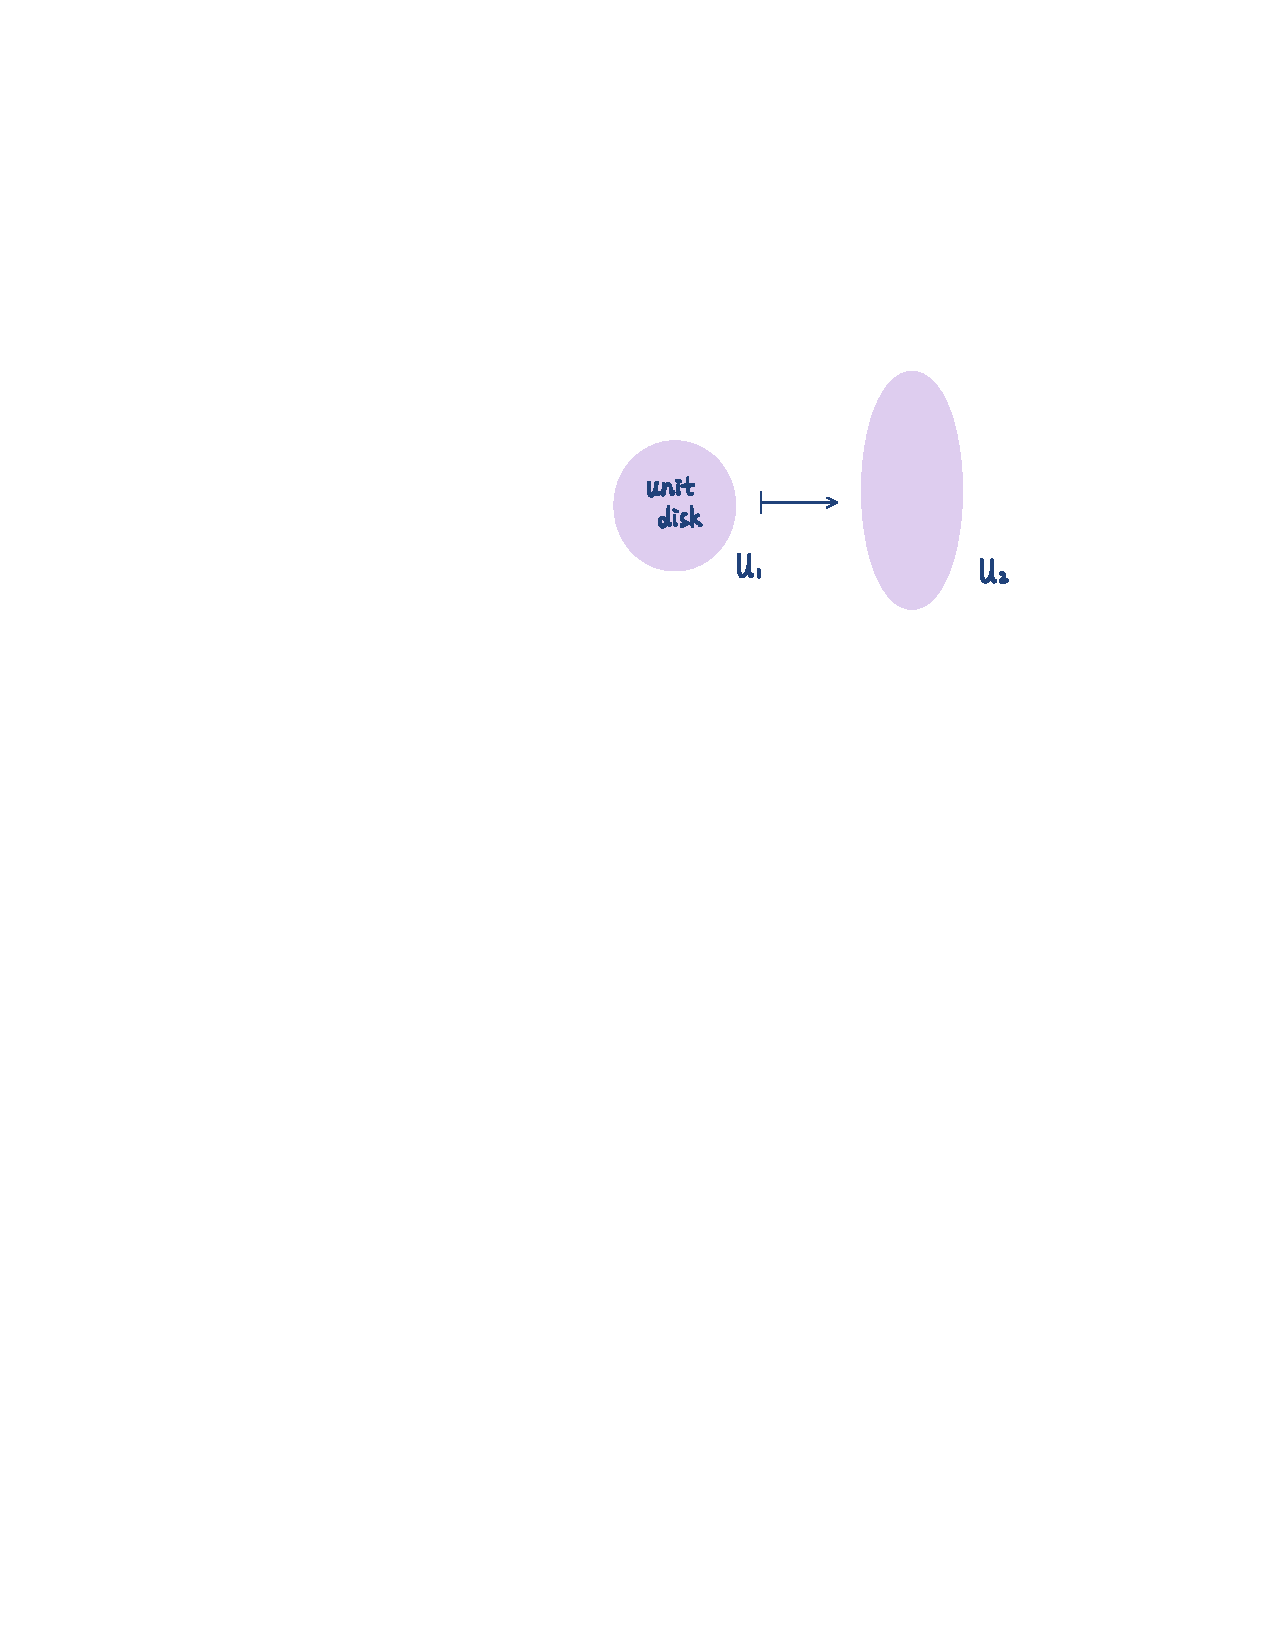
\includegraphics[scale=0.8]{manifold-disk.pdf}
\end{center}
$U_2$ is the image of the function $\alpha:U_1 \to U_2 \ \ \ (x,y) \mapsto (x,2y)$. Here we can write:
$$V_2(U_2)= 2V_2(U_1) \qquad \qquad \qquad \qquad V_1(\Bd(U_1)) = 2\pi$$
\hfill\break



\newpage
\section[Manifolds without Boundaries]{\color{red}Manifolds without Boundaries\color{black}}
\begin{defn}
Given $r,k,n \in \N$, a set $M \subseteq \R^n$ is called a k-manifold without boundary of class $C^r$ provided that for all $\vec{p} \in M$, there exist a set $V \subseteq M$ that contains $\vec{p}$, a set $U\subseteq \R^k$, with $V$ being open in $M$ and $U$ being open in $\R^k$, and a homeomorphism $\alpha \in C^r(U,V)$, with $rank(D\alpha(\vec{x})) = k$ for all $\vec{x}\in U$. The map $\alpha$ is called a coordinate patch on $M$ about $\vec{p}$.
\end{defn}

\example Consider the set $M = \{(x,y) \mid x^2 = y^3\}$, and the map $\alpha:\R \to M \ \ \ t \mapsto (t^3,t^2)$, here $\alpha $ is a homeomorphism, but $\alpha'(0) = 0$, so we have $rank(\alpha'(0)) = 0$. With such $\alpha$, $M$ is not a $1$-manifold, but $M \setminus \{(0,0)\}$ is a $1$-manifold. \\

\example Consider the set $M = \{(x,y) \mid y=|x| \}$. The map $\alpha:\R \to M \ \ \ t\mapsto (t^3, |t|^3)$ defines a homeomorphism, but $\alpha'(0) = 0$, so we have $rank(\alpha'(0)) = 0$. With such $\alpha$, $M$ is not a $1$-manifold. \\

\example Consider the set $M = \{(x,y) \mid y = x^2\}$. The map $\alpha:\R \to M \ \ \ t\mapsto (t^3,t^6)$ defines a homeomorphism, but $\alpha'(0) = 0$. The map $\widetilde{\alpha}:\R \to M \ \ \ t\mapsto (t,t^2)$ also defines a homeomorphism, and we have $\widetilde{\alpha}'(x) \neq 0$ for all $x \in \R$, here we found $\widetilde{\alpha}$ that satisfies the conditions that makes $M$ a $1$-manifold, and $\widetilde{\alpha}$ is called a coordinate patch on $M$\\

\example Check Section 23 Example 3 on Munkres Page 198.\\

\example Consider the set $M = \{(x,y) \mid x^2+y^2 = 1\}$. Note that continuous functions map compact set to compact set, here $M$ is compact, hence we cannot handle $M$ with a single coordinate patch, but we can make $M$ a $1$-manifold without boundary using the following four coordinate patches to cover all points on $M$:
$$\alpha_1: (-1,1) \to M \ \ \  x\mapsto \left(x,\sqrt{1-x^2}\right) \qquad\ \quad \alpha_2: (-1,1) \to M \ \ \  y\mapsto \left(\sqrt{1-y^2},y\right) $$
$$\alpha_3: (-1,1) \to M \ \ \  y\mapsto \left(-\sqrt{1-y^2},y\right)\qquad\ \quad \alpha_4: (-1,1) \to M \ \ \  x\mapsto \left(x,-\sqrt{1-x^2}\right)$$
\newpage

\example Consider the set $M=\{ \vec{x}\in \R^n \mid ||\vec{x}||=1\}$. One might use the following $2n$ coordinate patches to make $M$ a $n-1$-manifold:
\begin{align*}
&\alpha_1: \R^{n-1} \to \R^n \ \ \ (x_1,x_2,\cdots, x_{n-1})\mapsto \left(x_1,x_2,\cdots, x_{n-1}, \sqrt{1-\sum_{i=1}^{n-1} x_i^2}\right)\\
&\alpha_2: \R^{n-1} \to \R^n \ \ \ (x_1,x_2,\cdots, x_{n-1})\mapsto \left(x_1,x_2,\cdots, x_{n-1}, -\sqrt{1-\sum_{i=1}^{n-1} x_i^2}\right)\\
&\alpha_3: \R^{n-1} \to \R^n \ \ \ (x_1,x_2,\cdots, x_{n-1})\mapsto \left(x_1,x_2,\cdots, x_{n-2}, \sqrt{1-\sum_{i=1}^{n-1} x_i^2}\ , x_{n-1}\right)\\
&\alpha_4: \R^{n-1} \to \R^n \ \ \ (x_1,x_2,\cdots, x_{n-1})\mapsto \left(x_1,x_2,\cdots,x_{n-2}, -\sqrt{1-\sum_{i=1}^{n-1} x_i^2}\ ,x_{n-1}\right)\\
&{}\qquad\qquad\qquad\qquad\qquad\qquad\qquad\vdots\\
&\alpha_{2n-1}: \R^{n-1} \to \R^n \ \ \ (x_1,x_2,\cdots, x_{n-1})\mapsto \left(\sqrt{1-\sum_{i=1}^{n-1} x_i^2}\ ,x_1,x_2,\cdots, x_{n-1}\right)\\
&\alpha_{2n}: \R^{n-1} \to \R^n \ \ \ (x_1,x_2,\cdots, x_{n-1})\mapsto \left(-\sqrt{1-\sum_{i=1}^{n-1} x_i^2}\ ,x_1,x_2,\cdots, x_{n-1}\right)\\
\end{align*}

\hfill\break
\hfill\break
Let $M$ be a manifold. For $p\in M$, there might be two coordinate patches for $p$, $\alpha_1:U_1\to V_1$ and $\alpha_2:U_2\to V_2$, such that $\alpha_1(q_1) = p$ and $\alpha_2(q_2) = p$. 
\begin{center}
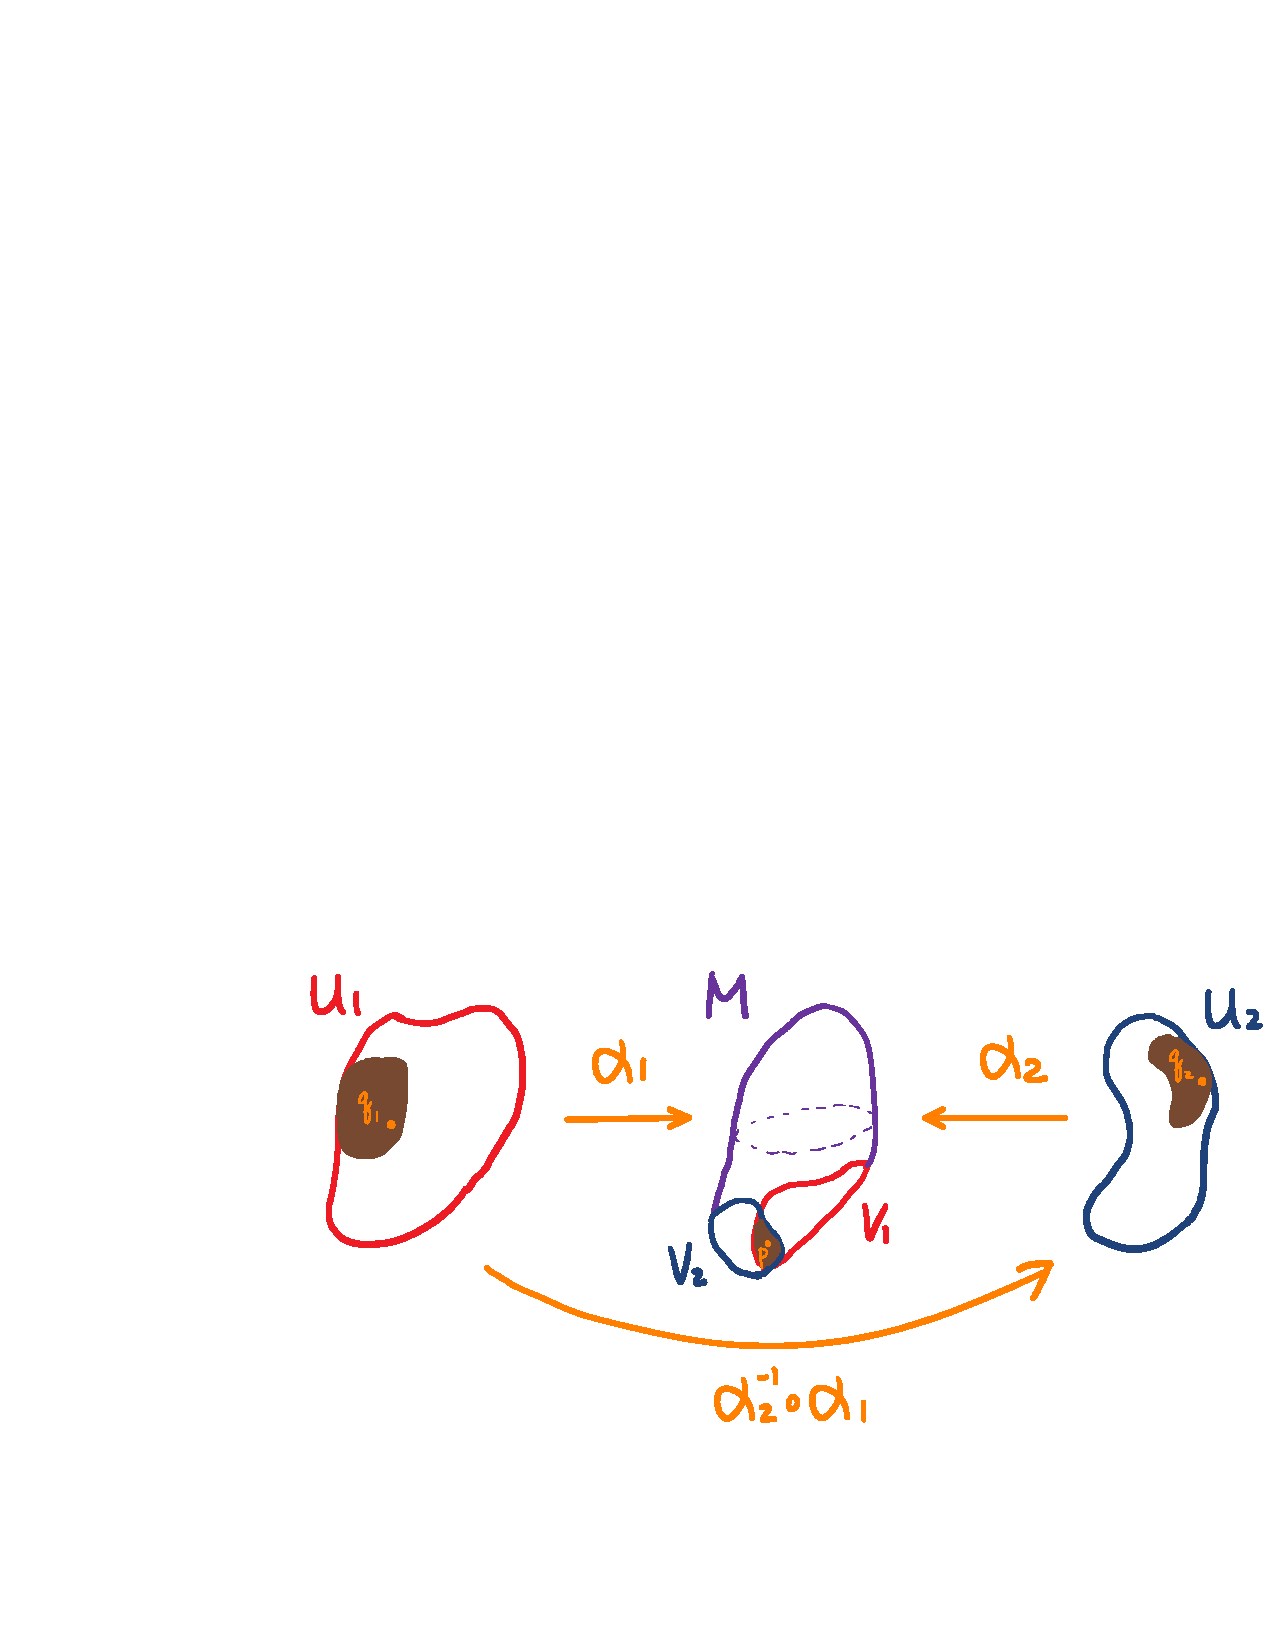
\includegraphics[scale=0.69]{coorPatch.pdf}
\end{center}
Here we note that $\alpha_2^{-1}\circ \alpha_1$ is of $C^r$ type when defined, and $(\alpha_2^{-1}\circ \alpha_1)^{-1} = \alpha_1^{-1} \circ \alpha_2$ is also of $C^r$ type. Hence we know that $\alpha_2^{-1}\circ \alpha_1$ is a $C^r$-diffeomorphism. \\
\newpage

\begin{thm}
For $M \subseteq  \R^n$, the followings are equivalent:
\begin{enumerate}[topsep=3pt,itemsep=-1ex,partopsep=1ex,parsep=1ex]
\item For all $\vec{p}\in M$, there exist a set $U\subseteq \R^k$ open in $\R^k$, a set $V \subseteq M$ open in \mbox{$M$ that contains $\vec{p}$,} and a homeomorphism $\alpha \in C^r(U,V)$ with rank $D\alpha(\vec{x}) = k$ for all $\vec{x}\in U$.  
\item For all $\vec{p}\in M$, there exist a set $A \subseteq \R^k$ open in $\R^k$, a set $V\subseteq M$ open in $M$ that \mbox{contains $\vec{p}$,} a function $g\in C^r(A,\R^{n-k})$, and a coordinate permutation $\rho:\R^n \to \R^n$, such that we have $\rho(V) = Graph(g)$.  
\end{enumerate}
\end{thm}
\begin{proof}
First we will show that (2) implies (1). Take $\alpha: A \to V \ \ \ \vec{x} \mapsto \rho^{-1}(\vec{x},g(\vec{x}))$. We see that $\alpha^{-1} = (\text{projection onto }\R^k)\circ \rho$ is a continuous function. This completes the proof for this direction. Now we will show that (1) implies (2). For $1 \leq s_1 < s_2 <\cdots, < s_k \leq n$ where $s_i \in \N$ for all $1\leq i\leq k$, let $\mathbb{S} = \{s_1,\cdots, s_k\}$. Define $P_\mathbb{S}:\R^n \to \R^k \ \ \ \vec{x}=(x_1,x_2,\cdots,x_n)\mapsto(x_{s_1},x_{s_2},\cdots,x_{s_k})$. Let $\vec{q}\coloneqq \alpha^{-1}(\vec{p})$. Here we can write $D(P_\mathbb{S}\circ \alpha)(\vec{q})= (DP_\mathbb{S}(\vec{p})) \cdot D\alpha(\vec{q}) = P_\mathbb{S}D\alpha(\vec{q}) = (k \text{ selected row of }D\alpha(\vec{q}))$. Hence we can choose $P_\mathbb{S}$ such that $D(P_\mathbb{S}\circ \alpha)$ is invertible. Let $\Omega$ denote the image of $P_\mathbb{S}$. By the Inverse Function Theorem, we can shrink $U,V, \Omega$ to $\widetilde{U},\widetilde{V},\widetilde{\Omega}$ such that $P_\mathbb{S}\circ \alpha$ is a diffeomorphism from $\widetilde{U}$ to $\widetilde{\Omega}$. Let $h = \alpha\circ (P_\mathbb{S}\circ \alpha)^{-1}$, note here we have $P_\mathbb{S}\circ h = P_\mathbb{S}\circ \alpha\circ (P_\mathbb{S}\circ \alpha)^{-1} = $ identity transformation. Let $\rho$ takes $\mathbb{S}$ to $\{1,\cdots, k\}$, one can check $\rho(\widetilde{V}) = Graph(h)$. This completes the proof.
\begin{center}
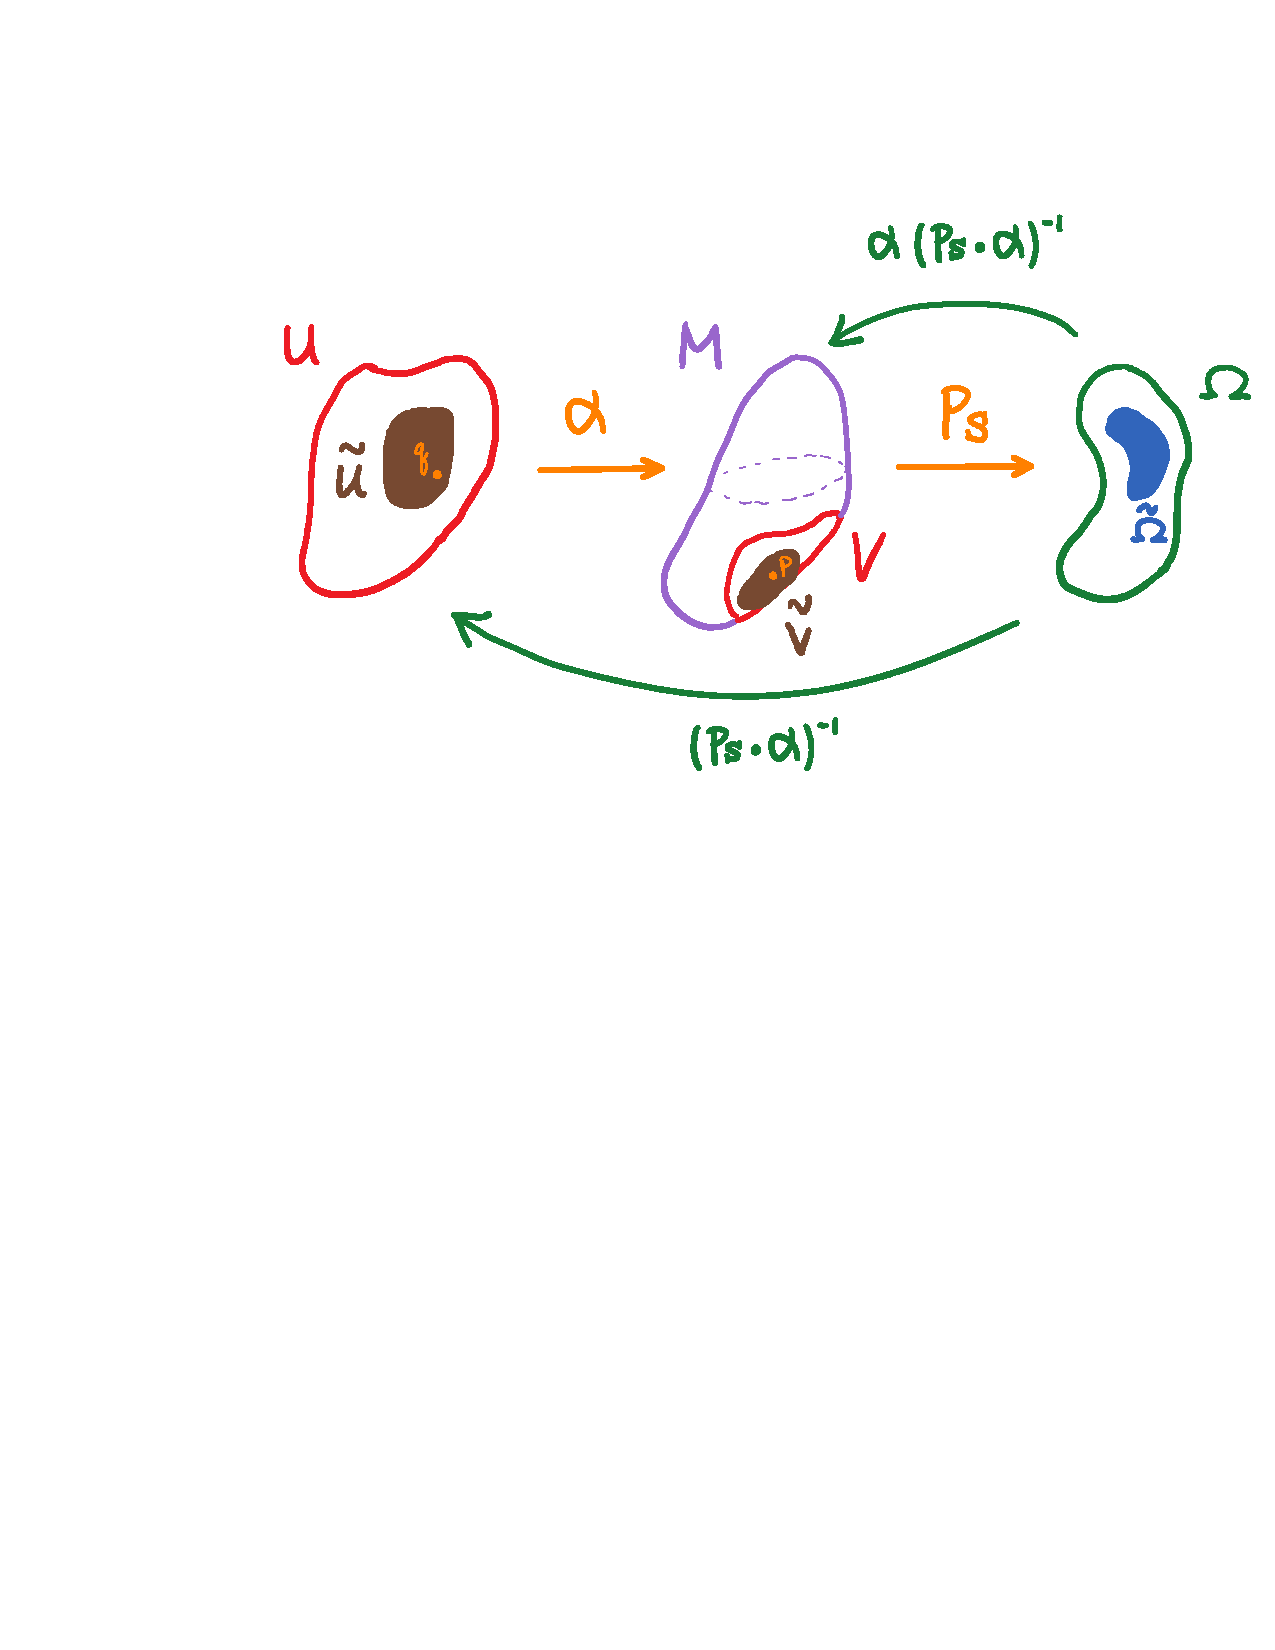
\includegraphics[scale=0.69]{manifoldsDefn.pdf}
\end{center}
\remark $(P_\mathbb{S} \circ \alpha)^{-1} \circ P_\mathbb{S} \in C^r(\rho^{-1}(\widetilde{\Omega}\times \R^{n-k} ),\widetilde{U})$.
\end{proof} 
 
In the settings of Theorem 16.1, a region of $M$ can be viewed as an affine set after a  dilation $\T_{\vec{p}}$ of the region of $M$ centered at $\vec{p}$, we denote this affine set by $\vec{p} + \T_{\vec{p}}(M)$, which is called the tangent space of $M$ at $\vec{p}$. For $\vec{x}$ near $\vec{q}$, we have:
$$\alpha(\vec{x}) \approx \alpha(\vec{q}) + D\alpha(\vec{q}) \cdot (\vec{x}-\vec{q})$$
We observe that $\T_{\vec{p}}(M)$ is approximately $D\alpha(\vec{q}) (\R^k)$. Now we suppose there is another coordinate patch $\that{\alpha}$ for $\vec{p}\in M$, with $\that{\alpha}(\vec{q}') = \vec{p}$. By Chain Rule, we can write:
$$D\that{\alpha}(\vec{q}')(\R^k) = (D\that{\alpha}(\vec{q}'))(D(\that{\alpha}^{-1}\circ \alpha )(\vec{q}))(\R^k) = D\alpha(\vec{q})(\R^k)$$

\begin{thm}
Let $U$ be an open subset of $\R^n$, let $F \in C^r(U,\R^{n-k})$, let $M = F^{-1}(\vec{0})$. 
If we have $rank(DF(\vec{x})) = n-k$ for all $\vec{x}\in M$, then $M$ is a $k$-manifolds without boundary of class $C^r$.
\end{thm}
\begin{proof}
One can apply the Implicit Function Theorem, and show that $M$ is locally a coordinate-permuted $C^r$ graph. Theorem 24.4 on Munkres provides a very similar proof.
\end{proof}

\note The converse of Theorem 16.2 might fail.\\

\note In the settings of Theorem 16.2 and Theorem 16.1, we have $F(\alpha(\vec{q})) = 0$ for all $\vec{q}$ in the domain of $\alpha$, hence by Chain Rule, we can write the following:
$$D(F\circ \alpha)(\vec{q}) = DF(\vec{p})\cdot D\alpha(\vec{q}) = 0 \qquad \Rightarrow \qquad \T_{\vec{p}}(M) = D\alpha(\vec{q})(\R^k) \subseteq \ker (DF(\vec{p}))$$
Here $D\alpha(\vec{q})(\R^k) $ has dimension $k$, and $\ker (DF(\vec{p}))$ has dimension $n-(n-k)= k$, so we have the following holds: 
$$\T_{\vec{p}}(M) = \ker (DF(\vec{p}))$$

\hfill\break
\exercise $F:\R^n \to \R \ \ \ \vec{x}\mapsto ||\vec{x}||^2 -1$. $F^{-1}(\vec{0})\coloneqq S^{n-1}$.\\
Here we have $DF(\vec{p}) = 2\cdot \vec{p}^T\Rightarrow \ker(DF(\vec{p})) = \{\vec{p}\}^\perp= \T_{\vec{p}}(S^{n-1})$.\\
\hfill\break


\remark Let $U$ be an open subset of $\R^{n+k}$, let $f\in C^1(U,\R^n)$ and $h \in C^1(U,\R)$, with $Df = n$. Each $f^{-1}(\vec{a})$ is a $k$-manifold without boundary by Theorem 16.2. Say we want to maximize, or minimize, $h$ under the constraint $f^{-1}(\vec{a})$. Lagrange Multiplier Theorem states that,if $h$ is maximized, or minimized at $\vec{x}$, we must have: $$f(\vec{x}) = \vec{a} \qquad\text{ with }\qquad Dh(\vec{x}) =\vec{\lambda}\cdot Df(\vec{x})$$ 
with some row vector $\vec{\lambda}$. If we vary $\vec{a}$, one might view the pair $(\vec{x},\vec{\lambda})$ as a function of $\vec{a}$ locally via Implicit Function Theorem. In the case where $n=1$, $\vec{a}\in \R$, here we denote $\vec{a}$ as scalar $a$, by argument above, $\vec{x}$ and $\lambda$ are functions of $a$. Here we have $f(\vec{x}(a)) = a$, with the following holds:
$$\frac{d}{da}h(\vec{x}(a)) = Dh(\vec{x}(a) ) \cdot \vec{x}'(a) = \lambda(a) Df(\vec{x}(a))\cdot \vec{x}'(a) = \lambda(a) \cdot \frac{d}{da}(f(\vec{x}(a))) = \lambda(a)$$

\newpage
\section[Manifolds which might have Boundaries]{\color{red}Manifold which might have Boundaries\color{black}}
\begin{defn}
For $S \subseteq \R^k$, $g:S \to \R^n$. For some $r \in \N$. $g$ is of $C^r$ type provided that there exists open subset of $\R^k$ that contains $S$, and $G \in C^r(U,\R^n)$ such that $G|_S = g$. If such $G$ exists, then $G$ extends $g$, and we write $g\in C^r(S,\R^n)$.
\end{defn}
\note Let $S\subseteq \R^k$, for $g\in C^r(S,\R^n)$, the extension $G$ of $g$ is not unique in general. For $|\alpha| \leq r$, we have $D^\alpha g \coloneqq D^\alpha G$ on $\Int(S)$ and on $\overline{\Int(S)}\cap S$. Suppose we have $g(S) \subseteq T \subseteq \R^n$, and let $h\in C^r(T,\R^m)$. We have $h\circ g \in C^r(S,\R^m)$. The extension $G$ of $g$ can be obtained through Whitney Extension Theorem, or, sometimes, simply by using the Taylor Polynomial. \\


\begin{defn}
$$\mathbb{H}^k\coloneqq \{(x_1,x_2,\cdots,x_k)\in \R^k \mid x_k \geq 0\} \qquad\qquad \mathbb{H}_+^k \coloneqq \{(x_1,x_2,\cdots,x_k)\in \R^k \mid x_k > 0\}$$
\end{defn}
\hfill\break
\begin{defn}
Given $r,k,n \in \N$, a set $M \subseteq \R^n$ is called a $k$-manifold of class $C^r$ provided that, for all $\vec{p}\in M$, there exist a subset $U$ of $\R^k$ open in either $\R^k$ or $\mathbb{H}^k$, a subset $V$ of $M$ open in $M$, and a homeomorphism $\alpha \in C^r(U,V)$ with $rank(D\alpha(\vec{x})) = k$ for all $\vec{x}\in U$. If such $\alpha$ exists for $\vec{p}\in M$, then $\alpha$ is called the coordinate patch on $M$ about $\vec{p}$, and $M$ is also called a $C^r$ manifold which might have  boundary. 
\end{defn}

\note Let $M$ be a $C^r$ manifold which might have  boundary, for $\vec{p}\in M$, let $\alpha_1$ and $\alpha_2$ be coordinate patches on $M$ about $\vec{p}$. Then $\alpha_1^{-1}$ is a $C^r$ function. $\alpha_2^{-1}\circ \alpha_1$ is a $C^r$ diffeomorphism between the domain of $\alpha_2^{-1} \circ \alpha_1$ and domain of $\alpha_1^{-1} \circ \alpha_2$. \\

Let $U$ and $W$ be relatively open in $\mathbb{H}^k$, let $\gamma:U \to W$ be a diffeomorphism.\\ 
Then $U \cap \mathbb{H}_+^k$ is open in $\R^k$. $D\gamma(\vec{x})$ is invertible for all $\vec{x}\in U\cap \mathbb{H}_+^k$. By the Inverse Function Theorem, $\gamma(U\cap \mathbb{H}_+^k)$ is open in $\mathbb{H}^k$ and must be contained in $\mathbb{H}_+^k$. Here we have $\gamma(U\cap \mathbb{H}_+^k) \subseteq (W \cap \mathbb{H}_+^k)$. With similar argument applying to $\gamma^{-1}$, we get $\gamma(U \cap \mathbb{H}_+^k) = W \cap \mathbb{H}_+^k$, so we have $\gamma(U\cap (\R^{k-1} \times \{0\}) = W\cap (\R^{k-1} \times \{0\})$. 


\begin{defn}
Let $M$ be a $k$-manifold. For $\vec{p}\in M$, $\vec{p}$ is called a boundary point of $M$ provided that there exists a coordinate patch $\alpha:U \to V$ on $M$ about $\vec{p}$ such that $U$ is open in $\mathbb{H}^k$, $V$ is open in $M$, and $\vec{p} = \alpha((x_1,x_2,\cdots, x_{k-1},0))$. The set of boundary points of $M$ is called the manifold boundary of $M$. denoted as $\partial M$. For $\vec{q}\in M\setminus \partial M$, $\vec{q}$ is called an interior point of $M$. 
\end{defn}

\begin{lem}
Let $M$ be a $k$-manifold in $\R^n$, and let $\alpha:U \to V$ be a coordinate patch about the point $\vec{p}\in M$. If $U$ is open in $\mathbb{H}^k$ and $\vec{p} = \alpha(\vec{x})$ for some $\vec{x}\in \mathbb{H}_+^k$, then $\vec{p}$ is an interior point of $M$. If $U$ is open in $\R^k$, then $\vec{p}$ is an interior point of $M$. 
\end{lem}

\newpage
\begin{thm}[Theorem 24.4 on Munkres]
Let $M$ be a $k$-manifold, $\partial M$ is a $C^r$ $(k-1)$-manifold without boundary.
\end{thm}
\begin{proof}
For coordinate patch $\alpha:U \to V$ where $V \subseteq M$, it induces coordinate patch defined by the following: 
\begin{align*}
\hat{\alpha}: \{(x_1,x_2,\cdots, x_{k-1})\mid (x_1,x_2,\cdots, x_{k-1},0) \in U\}&\to \partial M \\ (x_1,x_2,\cdots, x_{k-1})&\mapsto \alpha(x_1,x_2,\cdots, x_{k-1},0)
\end{align*}
\end{proof}

\exercise For $k$-manifold $M_1$ and $M_2$ in $\R^n$. If there exists a diffeomorphism defined by $\alpha:M_1 \to M_2$, then $\alpha|_{\partial M_1}$ is a diffeomorphism from $\partial M_1$ to $\partial M_2$.\\

\example Let $M$ be a $k$-manifold in $\R^n$. Consider the extreme case where we have $k=n$, $n$-manifold without boundary is an open subset of $\R^n$. $n$-manifold which might have boundary is an open subset of $\R^n$ union with a set $\partial M$ that is an $n-1$-manifold without boundary, and $\partial M$ is contained in the topological boundary of $M$. \\

\example
Consider a closed triangle in $\R^2$, which is not a $2$-manifold, because the boundary of the closed triangle fails to be a 1-manifold. If we take out the vertices of the closed triangle, that becomes a $2$-manifold. If we take out all boundary points of the closed triangle, then we get a 2-manifold without boundary.\\

\hfill\break
Here we extend the definition for $k$-manifolds in $\R^n$ for the case where $k=0$: \begin{defn} 
A countable collection of of points in $\R^n$ is called a $0$-manifold in $\R^n$.
\end{defn}

\remark $0$-manifold $M$ has $\partial M = \emptyset$. $M$ is a $0$-manifold if and only if each singleton subset of $M$ is relatively open, that is, if and only if each point of $M$ is isolated. \\

\note A set $M$ is a compact $0$-manifold $\iff$ $M$ is a finite set. For such we write: $$\int_M fdV \coloneqq \sum_{x \in M} f(x)$$
\note All $0$-manifolds are countable sets. \\

\exercise For open subset $U$ of a $k$-manifold $M$, $U$ is a $k$-manifold.\\

\begin{thm}
Every $k$-manifold $M$ can be decomposed uniquely as a disjoint union of open connected $k$-manifolds, which are called the components of $M$. 
\end{thm}
\begin{proof}
The proof of this theorem can be found on Math 395 Supplement materials Section $H$.
\end{proof}

\newpage
\begin{thm}
Every connected 1-manifold of class $C^r$ is $C^r$-diffeomorphic to an interval in $\R$ or to the circle $S^1$. 
\end{thm}
\begin{proof}[Outline of the proof]
Suppose $M$ is a connected $1$ manifold. Let $x_0 \in M \setminus \partial M$. One might want to prove the following exercise:\\

\exercise For any $x_1 \in M\setminus\{ x_0\}$, there is $I \subseteq M$ such that $I$ is homeomorphic to closed interval with $\partial I = \{ x_0,x_1\}$, this can be viewed as a path connecting $x_0$ and $x_1$, one can mimic the proof of Math 395 HW3 Q4 to construct such path.\\

Now consider the following two cases:\\
(1) There exists only one such $I$ connecting $x_0$ and $x_1$ for each $x_1\in M\setminus\{ x_0\}$. Denote such $I$ as $I_{x_0,x_1}$. Consider a partition of $M\setminus \{x_0\}$ into two subsets, one is called the left of $x_0$ and the other one is called the right of $x_0$. $x_1 \in M\setminus \{x_0\}$ belongs to left or right of $x_0$ according to whether $I_{x_0,x_1}$ is contained in the left of $x_0$ union with $\{x_0\}$, or the right of $x_0$ union with $\{x_0\}$, as defined by the following:

\begin{center}
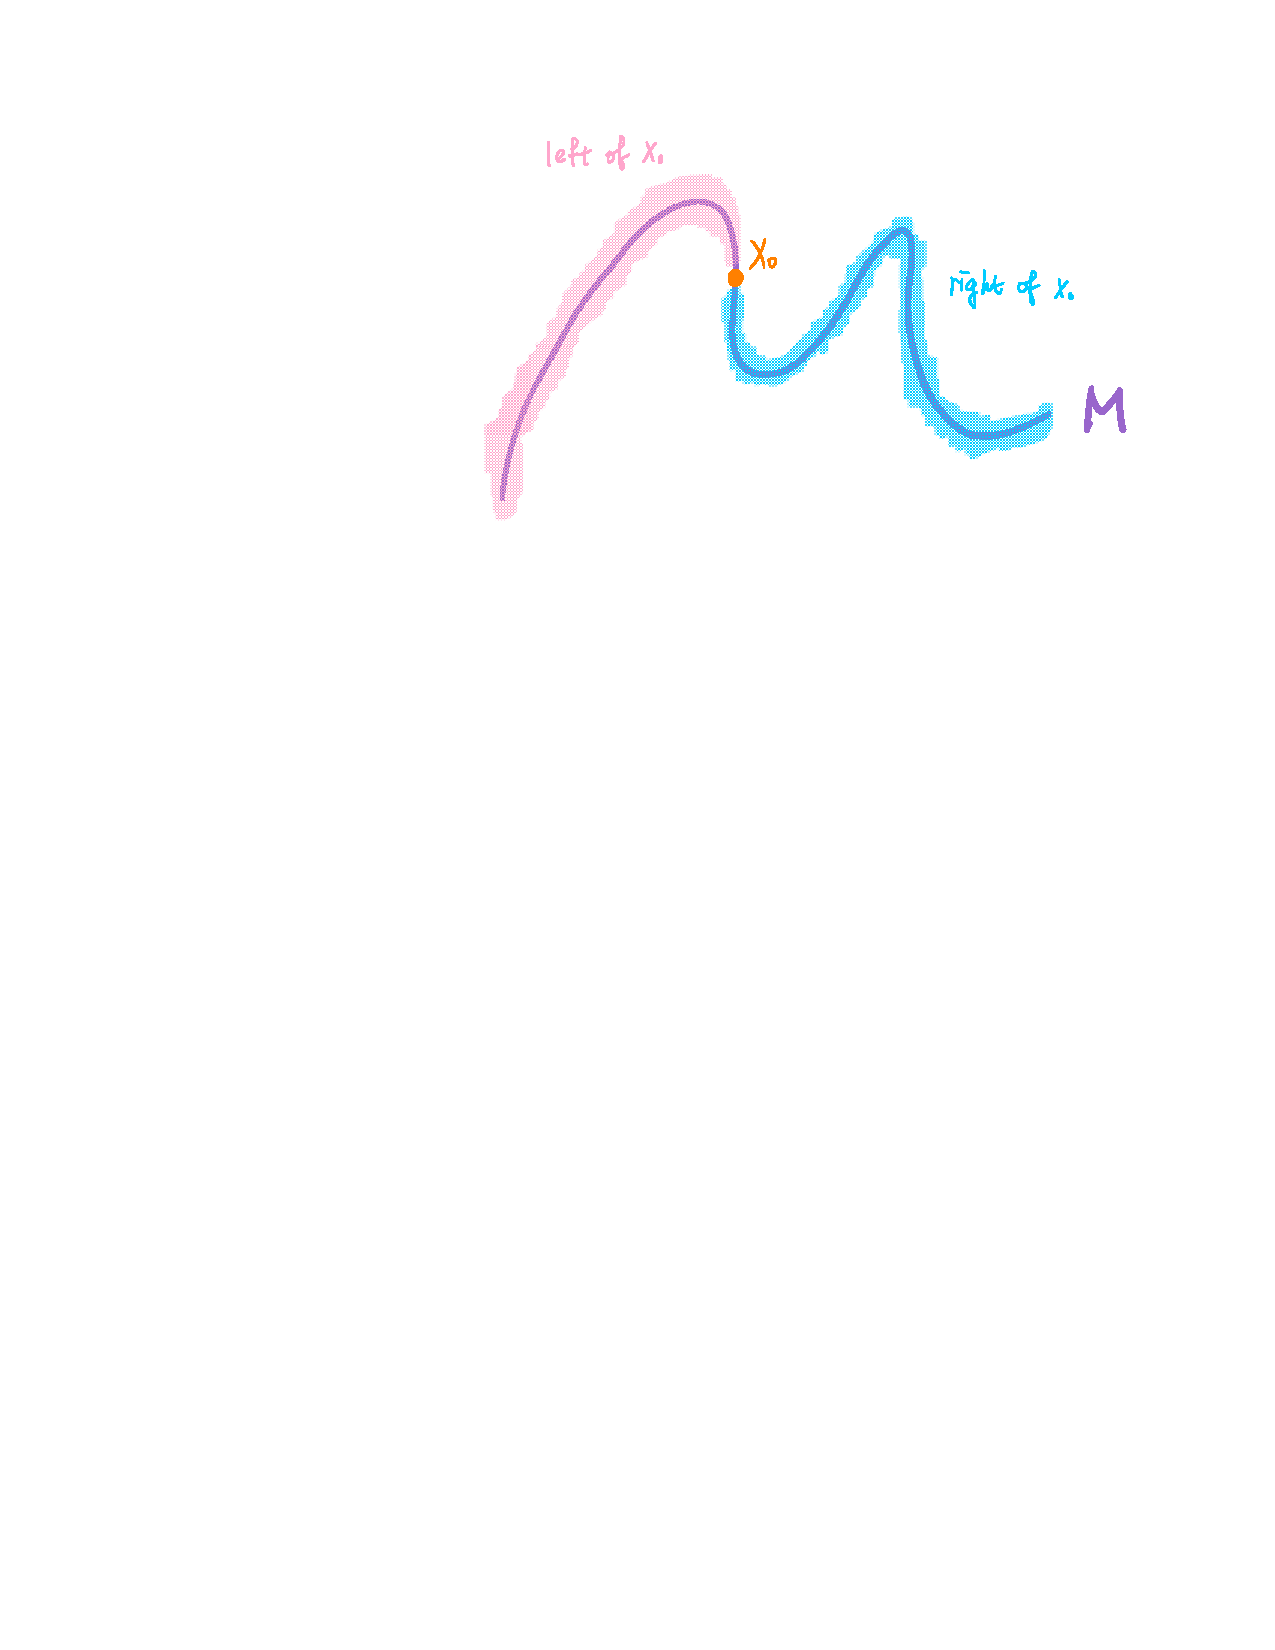
\includegraphics[scale=0.5]{1-manifoldHom.pdf}
\end{center}

Now consider a function $f:M \to \R$ defined by the following: 
$$f:M \to \R \ \ \ x_1\mapsto\begin{cases} 0 & x_1 = x_0 \\ V_1(I_{x_0,x_1}) & x_1\text{ lies on the right of }x_0 \\ -V_1(I_{x_0,x_1}) & x_1\text{ lies on the left of }x_0\end{cases}$$ 
One can check that $f:M \to \R$ is continuous, and here $f(M)$ is connected because $M$ is connected, then we know that $f(M)$ must be an interval. Consider the following exercise:\\

\exercise\\ 
The set $\{y \in f(M)\mid \#(f^{-1}(y)) = 1\}$ is open in $f(M)$, closed in $f(M)$, and contains $0$. \\

with this exercise, we know that $f:M \to f(M)$ is a continuous bijection. Consider coordinate patch $\alpha: U \to V \subseteq M$ with $U$ being an interval and $[t_0,t_1] \subseteq U$, we have $f(\alpha(t_2))$ either being greater than or less than $f(\alpha(t_1))$. WLOG, we suppose $f(\alpha(t_2)) > f(\alpha(t_1))$. We can write the following:
$$\int_{[t_1,t_2]} ||D\alpha|| = \int_{[t_1,t_2]} \mathcal{V}(D\alpha) = V_1(\alpha([t_1,t_2])) = f(\alpha(t_2)) - f(\alpha(t_1))$$
Then by the Fundamental Theorem of Calculus, we see that $D(f\circ \alpha) = ||D\alpha||$. From the definition of coordinate patch, we know that $D(f\circ \alpha) = ||D\alpha|| > 0$. Here $D\alpha$ and $||D\alpha||$ are both $C^{r-1}$ functions, note that the norm function is of $C^\infty$ type except at $\vec{0}$, but $D\alpha$ is nonzero. Then we know that $D(f\circ \alpha)$ is of $C^{r-1}$ type and hence $f\circ \alpha$ is of $C^r$ type. Hence $f = (f\circ \alpha) \circ \alpha^{-1}$ is also of $C^r$ type.  Since $D(f\circ \alpha) \neq 0$, then by Inverse Function Theorem, we know that $(f\circ \alpha)^{-1}$ is of $C^r$ type, and hence $f^{-1} = \alpha \circ (f\circ \alpha)^{-1}$ is also of $C^r$ type. This completes the proof for case (1).\\

Now consider case (2), in which case there exists $I_1, I_2 \subseteq M$ that are homeomorphic to closed intervals in $\R^2$ with $\partial I_1 = \{x_0,x_1\} = I_2$ and $I_1 \neq I_2$, for some $\vec{x}_1 \in M\setminus\{x_0\}$. WLOG, here we assume $I_1 \nsubseteq I_2$. We will make use of the following exercises:\\

\exercise $I_1 \setminus I_2$ is relatively open in $I_1 \setminus \partial I_1$, relatively closed in $I_1 \setminus \partial I_1$, and nonempty.\\

From this exercise, we know that $I_1 \setminus I_2 = I_1 \setminus \partial I_1$, hence we have $I_1 \cap I_2 = \{x_0,x_1\}$. \\

\exercise $I_1 \cup I_2$ is relatively open in $M$, relatively closed in $M$, and non-empty.\\

With these exercises, we conclude that $M = I_1\cup I_2$. From similar constructions in case (1), one can obtain the following $C^r$-diffeomorphisms:
\begin{align*}
f_1&:I_1 \to [0, V_1(I_1)] \ \ \ \vec{x}_2\mapsto V_1(I_{x_0,x_2})\\
f_2&:I_2 \to [-V_1(I_2),0] \ \ \ \vec{x}_2\mapsto -V_1(I_{x_0,x_2})
\end{align*}


Let $l_1\coloneqq  V_1(I_1) $ and $l_2 \coloneqq V_1(I_2)$, and consider the following map:
$$\mu:M \to \R^2 \ \ \ \vec{x} \mapsto \begin{cases}\left(\cos\frac{2\pi f_1(\vec{x})}{l_1+l_2}, \sin\frac{2\pi f_1(\vec{x})}{l_1+l_2}\right) & \vec{x}\in I_1\\
\left(\cos\frac{2\pi f_2(\vec{x})}{l_1+l_2}, \sin\frac{2\pi f_2(\vec{x})}{l_1+l_2}\right) & \vec{x}\in I_2\\
\end{cases}$$
One can verify that $\mu$ defines a diffeomorphism from $M$ to $S^1$.
\end{proof}


\begin{corT}
Every connected $1$-manifold is differomorphic to one of the followings:
$$1.\ \ (0,1) \qquad\qquad\qquad
2.\   \ [0,1] \qquad\qquad\qquad
3.\   \ [0,1)\qquad\qquad\qquad
4.\   \ S^1$$
\end{corT}
\begin{proof}
Use the arctangent function and some affine maps. For the uniqueness, we note that diffeomorphism preserves compactness, and also note that if two 1-manifolds are diffeomorphic, then their boundary points of manifolds are also diffeomorphic to each other, hence the manifold boundaries of these two $1$-manifolds have the same cardinality. 
\end{proof}

\newpage
\begin{thm}
Every compact connected $2$-manifold without boundary in $\R^3$ is diffeomorphic to a sphere in $\R^3$, or a sphere glued with some handles.
\begin{center}
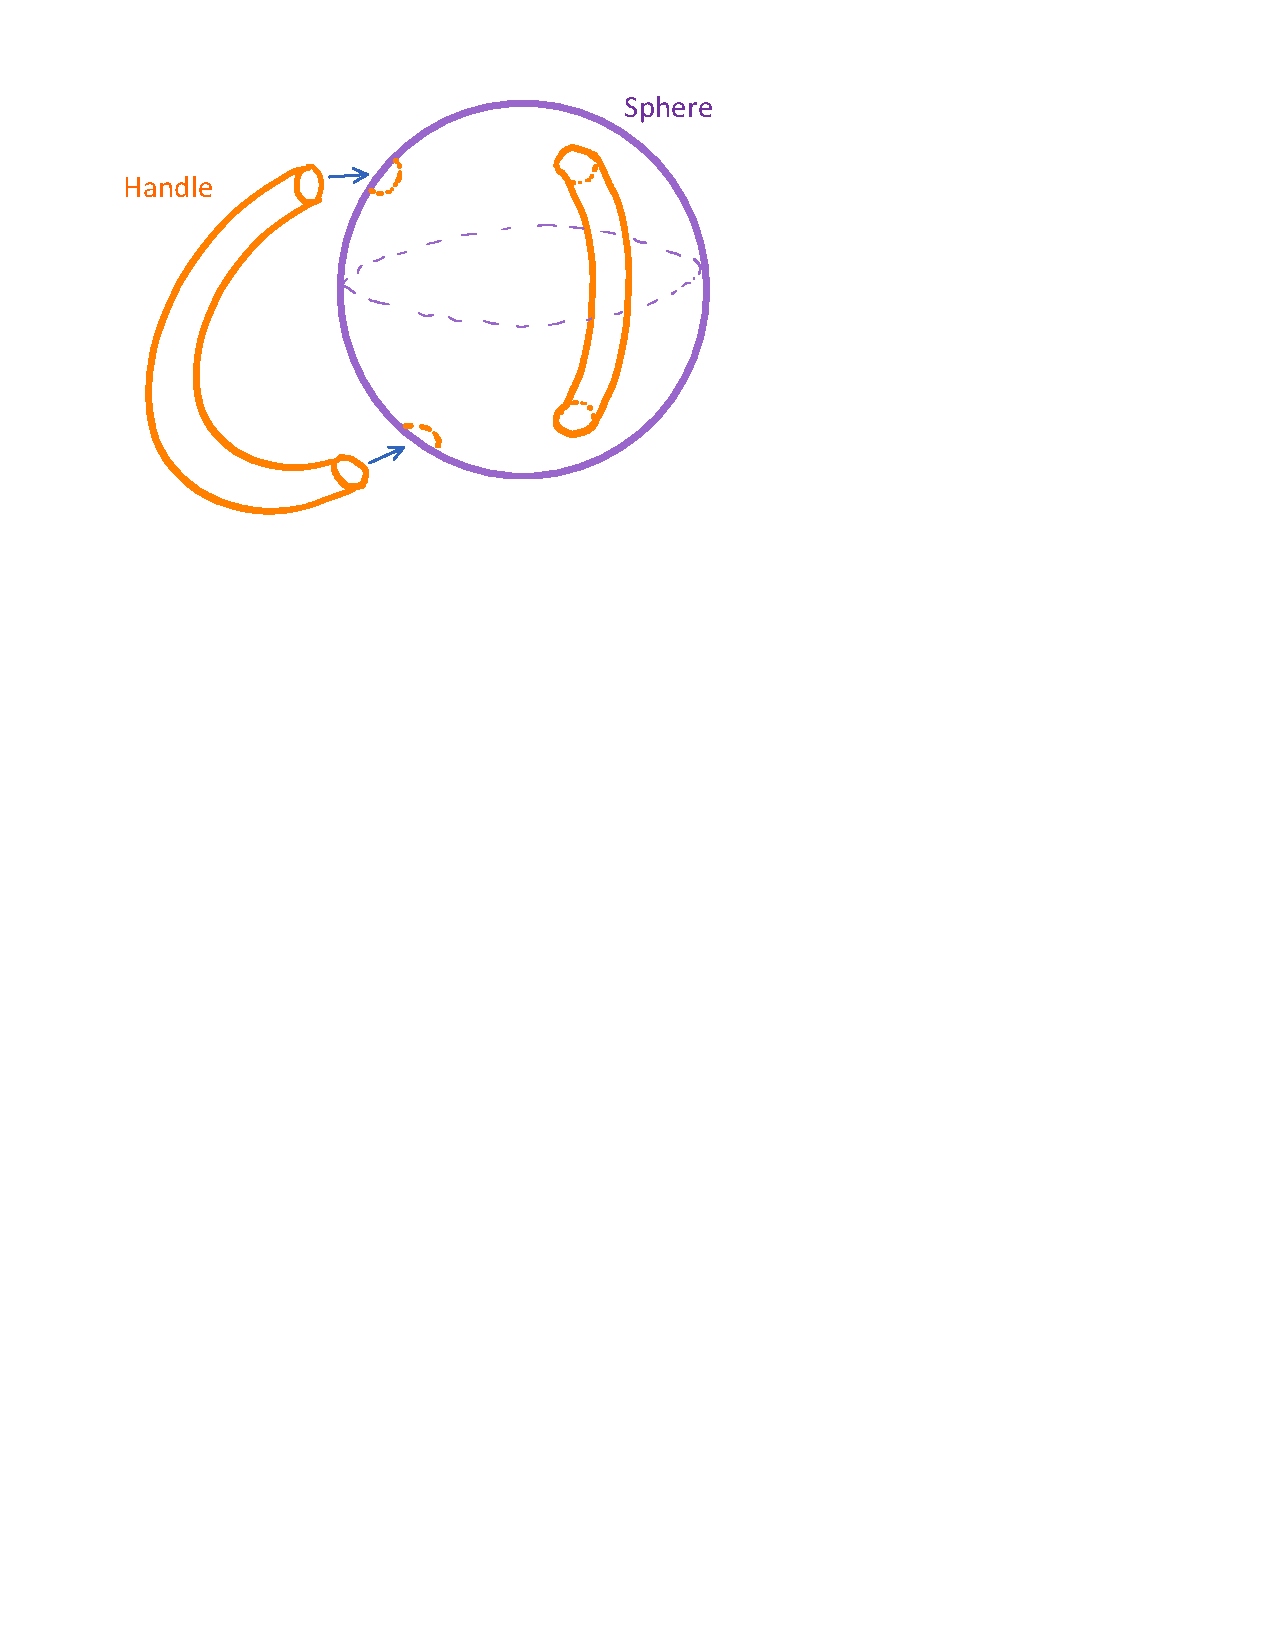
\includegraphics[scale=0.8]{handleBody.pdf}
\end{center}
\end{thm}

If a $2$-manifold with boundary lives in $\R^4$ or higher dimensions, one can glue a disk along the boundary of a Mobius strip to get a projective plane.\\

\begin{thm}
More generally, every compact connected $2$-manifold without boundary in $\R^n$ is diffeomorphic to one of these with handles: (1) a sphere with handles, (2) a projective plane, (3) a Klein bottle.
\end{thm}

One can glue two disks to get a sphere $S^2$ in $\R^3$, glue a disk to boundary of Mobius strip to get a projective plane in $\R^4$, and glue two Mobius strip to get a Klein Bottle in $\R^4$.








\newpage
\section[One-forms and Pullbacks]{\color{red}One-forms and Pullbakcs\color{black}}
\begin{defn}
A $1$-form on an open subset $A$ of $\R^n$ is a continuous function from $A$ to $\R^n_{row}$
\end{defn}

\note Here $R^n_{row}$ is the space of vectors in $\R^n$ represented by row vector. \\

\remark For notation, one might write $(\R^n)^* \coloneqq R^n_{row}$.\\

\example Let $A$ be an open subset of $\R^n$. For $f \in C^1(A,\R)$, the function $Df$ which maps $\vec{x}$ to $Df(\vec{x})$ is a $1$-form. In multivariate differentiation, the operator $D$ takes functions defined on some open subset of $\R^n$ to matrices in $Mat(m,n)$. In the case we $m=1$, we denote the operator $D$ as $d$, which takes functions defined on some open subset of $\R^n$ to $1$-forms.\\

\begin{defn}
Let $A$ be an open subset of $\R^n$, $B$ be an open subset of $\R^m$, let $\alpha \in C^1(B,A)$, and let $\omega$ be an $1$-form defined on $A$.  $\alpha^*\omega \coloneqq (\omega\circ \alpha) \cdot D\alpha$ is called the pullback of $\omega$ by $\alpha$. 
\end{defn}

\remark In the settings of definition 18.0.0.0.2, $\omega\circ \alpha$ is an $1 \times n$ matrix and $D\alpha$ is an $n \times m$ matrix, hence $\alpha^*\omega$ is an $1 \times m$ matrix, which is an $1$-form on $B$.\\

\note For $\R$-valued function $f$ defined on an open subset $A$ of $\R^n$, and $\alpha\in C^1(B,A)$ where $B$ is an open subset of $\R^m$, we can write the following: 
$$\alpha^*df = (df\circ \alpha)\cdot D\alpha =(Df\circ \alpha)\cdot D\alpha = D(f\circ \alpha) = d(f\circ \alpha)$$ 
%Since we have $f\circ \alpha = \alpha^*f$, so $\alpha^*df = d(\alpha^*f)$. \\
\note \textbf{Fundamental Theorem of Calculus II for one-forms}\\
For $C^1$ type function $\alpha:[a,b]=I \to A$ where $A$ is an open subset of $\R^n$, with $\omega$ being an $1$-form on $A$. Then $\alpha^*\omega$ is a $1$-form on $I$, which can be viewed as $\R$-valued function. Consider the $1$-manifold $Y_\alpha$, we can define the following:
$$\int_{Y_\alpha} \omega \coloneqq \int_I \alpha^*\omega$$
For $C^1$ type function $f$ defined on $A$, we can write the following: 
\begin{align*}
\int_{Y_\alpha} df = \int_I \alpha^*df = \int_I d(f\circ \alpha) = \int_I (f\circ \alpha)' 
&= (f\circ \alpha)(b) - (f\circ \alpha) (a) \\
&= f(\alpha(b)) - f(\alpha(a))\coloneqq \Delta_{Y_\alpha}f
\end{align*}
Here we get the results by the Fundamental Theorem of Calculus II. \\


\example Let $A$ be an open subset of $\R^n$. For $f\in C^1(A,\R)$, $df:\vec{x} \to Df(\vec{x})$ is a $1$-form. We write the following:
\begin{align*}
df &= \bmat{\frac{\partial f}{\partial x_1}&\frac{\partial f}{\partial x_1} &\cdots& \frac{\partial f}{\partial x_n}}\\ &= \frac{\partial f}{\partial x_1}\bmat{1&0&\cdots&0} + \frac{\partial f}{\partial x_2}\bmat{0&1&0&\cdots&0} + \cdots + \frac{\partial f}{\partial x_n}\bmat{0&0&\cdots&1} \\&= \frac{\partial f}{\partial x_1} dx_1 + \frac{\partial f}{\partial x_2 }dx_2 + \cdots + \frac{\partial f}{\partial x_n}dx_n
\end{align*}
Here $dx_i \coloneqq d\pi_i$, where $\pi_i : \R^n \to \R \ \ \ (x_1,x_2,\cdots, x_n)\mapsto x_i$ is the projection function.
In general, for $1$-form defined on $A$, we write the following: 
$$\omega = \bmat{\omega_1 &\omega_2 &\cdots &\omega_n} = \omega_1 dx_1 +\omega_2 dx_2 + \cdots + \omega_n dx_n$$

\begin{defn}
Let $f:\R^n \to \R$ be a $C^1$ function, and let $\alpha:\R^m \to \R^n$, we write $\alpha^{*,0}f = f\circ \alpha$.
\end{defn}


\note In the settings of Definition 18.0.0.3, $\alpha^*df = d(\alpha^{*,0}f)$\\

\note Let $\omega$ be a $1$-form defined on open subset $A$ of $\R^n$, let $B$ be an open subset of $\R^m$, let $C$ be open subset of $\R^k$, and let $\alpha_1 \in C^1(A,B)$, and let $\alpha_2 \in C^1(B,C)$, we have: 
$$(\alpha_2 \circ \alpha_1)^*\omega = \alpha_1^*(\alpha_2^*\omega)$$

\example Consider the map $\alpha:\R^2 \to \R^2$ defined by $(r,\Phi) \mapsto (r\cos(\Phi), r\sin(\Phi))$. \\We can write the following:
\begin{align*}
\alpha^* \left(\frac{x_1}{x_1^2+x_2^2}dx_1 + \frac{x_2}{x_1^2+x_2^2}dx_2  \right)=&\frac{r\cos(\Phi)}{r^2}d(r\cos(\Phi)) + \frac{r\sin(\Phi)}{r^2}d(r\sin(\Phi))\\
=&+\frac{r\cos(\Phi)}{r^2}(\cos(\Phi)dr - r\sin(\Phi) d\Phi)\\
 &+ \frac{r\sin(\Phi)}{r^2}(\sin(\Phi) dr + r\cos(\Phi)d\Phi)\\
=&\frac{1}{r}dr
\end{align*}
Similarly, we have:
$$\alpha^*  \left(\frac{-x_2}{x_1^2+x_2^2}dx_1 + \frac{x_1}{x_1^2+x_2^2}dx_2  \right)=\frac{r\cos(\Phi)}{r^2}d(r\cos(\Phi)) + \frac{r\sin(\Phi)}{r^2}d(r\sin(\Phi)) = d\Phi$$


\remark Suppose $\omega:[a,b]\to \R$ is a $1$-form on $[a,b]$. Here we can write the following:
$$\int_{[a,b]} \omega = \int_a^b \omega$$


\note Let $I,J$ be intervals of $\R$ such that $\beta:I\to J$ defines a diffeomorphism. \\
For $\alpha \in C^1(I,\R^n)$, let $\omega$ be a $1$-form defined on $Y_\alpha$, we can write the following:
\begin{align*}
\int_{Y_{\alpha\circ \beta}} \omega &= \int_{J} (\alpha\circ \beta)^*\omega =\int_J \beta^*\alpha^*\omega = \int_J ((\alpha^*\omega) \circ \beta)\cdot D\beta
\end{align*}
Here we see that $D\beta = \det(D\beta)$ because $D\beta$ is a $1\times 1$ matrix. Also note that, since $\beta$ defines a diffeomorphism, then $D\beta(x)\neq 0$ for all $x \in J$, and $D\beta$ is continuous, hence $D\beta$ is a negative, or positive function. Then by the Change of Variable Theorem, we can write the following:
\begin{align*}
\int_{Y_{\alpha\circ \beta}} \omega &= \int_J ((\alpha^*\omega) \circ \beta)\cdot D\beta = \begin{cases}\int_I \alpha^*\omega & D\beta(x) > 0,\ \forall x \in J\\\ -\int_I \alpha^*\omega & D\beta(x) < 0,\ \forall x \in J \end{cases}
\end{align*}
On the other hand, we have:
\begin{align*}
\int_{Y_\alpha} \omega = \int_{I} \alpha^*\omega 
\end{align*}
Combining, we can write the following:
\begin{align*}
\int_{Y_{\alpha\circ \beta}} \omega = \begin{cases}\int_{Y_\alpha} \omega & D\beta(x) > 0,\ \forall x \in J\\\ -\int_{Y_\alpha} \omega & D\beta(x) < 0,\ \forall x \in J \end{cases}
\end{align*}

\note For $1$-form $\omega$ defined on open subset $A$ of $\R^n$, and $\alpha\in C^1([a,b] \to A)$, we have:
\begin{align*}
\int_{Y_\alpha} \omega &= \int_{Y_\alpha} \omega_1dx_1+\omega_2dx_2+\cdots +\omega_n dx_n \\&= \int_{I} (\omega_1\circ \alpha)\cdot  D\alpha_1 + (\omega_2\circ \alpha)\cdot  D\alpha_2
+\cdots + (\omega_2\circ \alpha)\cdot  D\alpha_2
\end{align*}

\example In Physics, a force field can be described by a $1$-form $\omega$ defined on an open subset $A$ of $\R^n$. Let $I\subseteq \R$ be an interval, and let $\alpha\in C^1(I,A)$, then $\alpha$ can be viewed as a path of a particle in the $\R^n$ space. The formula $\int_{Y_\alpha} \omega$ describes the work acted on the particle through the path $Y_\alpha$.\\

\example Consider $\alpha : [0,1]\to \R^n \ \ \ t\mapsto (t,t^n)$.\\ Let $\pi_1:\R^2 \to \R \ \ \ (x,y)\mapsto x$, $\pi_2:\R^2 \to \R \ \ \ (x,y)\mapsto y$ be the projection functions, we can write the following:
\begin{align*}
\int_{Y_\alpha} \pi_2\, d\pi_1 - \pi_1\, d\pi_2 = \int_0^1 t^n  - n t^{n} = \frac{1-n}{n+1}
\end{align*}

\begin{prop}
Let $f:[a,b]\to \R^n$, the followings are equivalent:
\begin{enumerate}[topsep=3pt,itemsep=-1ex,partopsep=1ex,parsep=1ex]
\item There exists a function $g\in C^k(A,\R^n)$ such that $g(x) = f(x)$ for $x\in [a,b]$, with $A$ being an open subset of $\R$ that contains $[a,b]$.
\item $f \in C([a,b])$, with $f|_{(a,b)} \in C^k((a,b),\R^n)$, both $\lim_{t \to a^+} f^{(j)}(t)$ and $\lim_{t \to b^-}f^{(j)}(t)$ exist and are finite for $j\in \N$ with $1\leq j \leq k$.
\end{enumerate}
\end{prop}
\begin{proof}
It is trivial to show that (1) implies (2). For (2) implies (1), one can use the Taylor Polynomials to extend the function $f$. 
\end{proof}

\begin{defn}
For interval $[a,b]\subseteq \R$, a function $f:[a,b] \to \R^n$ is said to be of $C^k$ type provided that there exists a function $g\in C^k(A,\R^n)$ such that $g(x) = f(x)$ for $x\in [a,b]$, with $A$ being an open subset of $\R$ that contains $[a,b]$. In such case, we write $f \in C^k([a,b],\R^n)$. 
\end{defn}

\begin{defn}
For interval $[a,b]\subseteq \R$, a function $f:[a,b] \to \R^n$ is said to be of piecewise $C^k$ type provided that $f$ is continuous on $[a,b]$, and $f|_{[t_{j-1},t_j]} \in C^k([t_{j-1},t_j],\R^n)$ for each $j$, where $\{t_1,t_2,\cdots, t_m\}$ defines a partition on $[a,b]$. In such case, we write $f \in C_{pw}^k([a,b],\R^n)$. 
\end{defn}

\example The function $M:[a,b]\to \R^2$ defined by the following is of piecewise $C^k$ type. 
\begin{center}
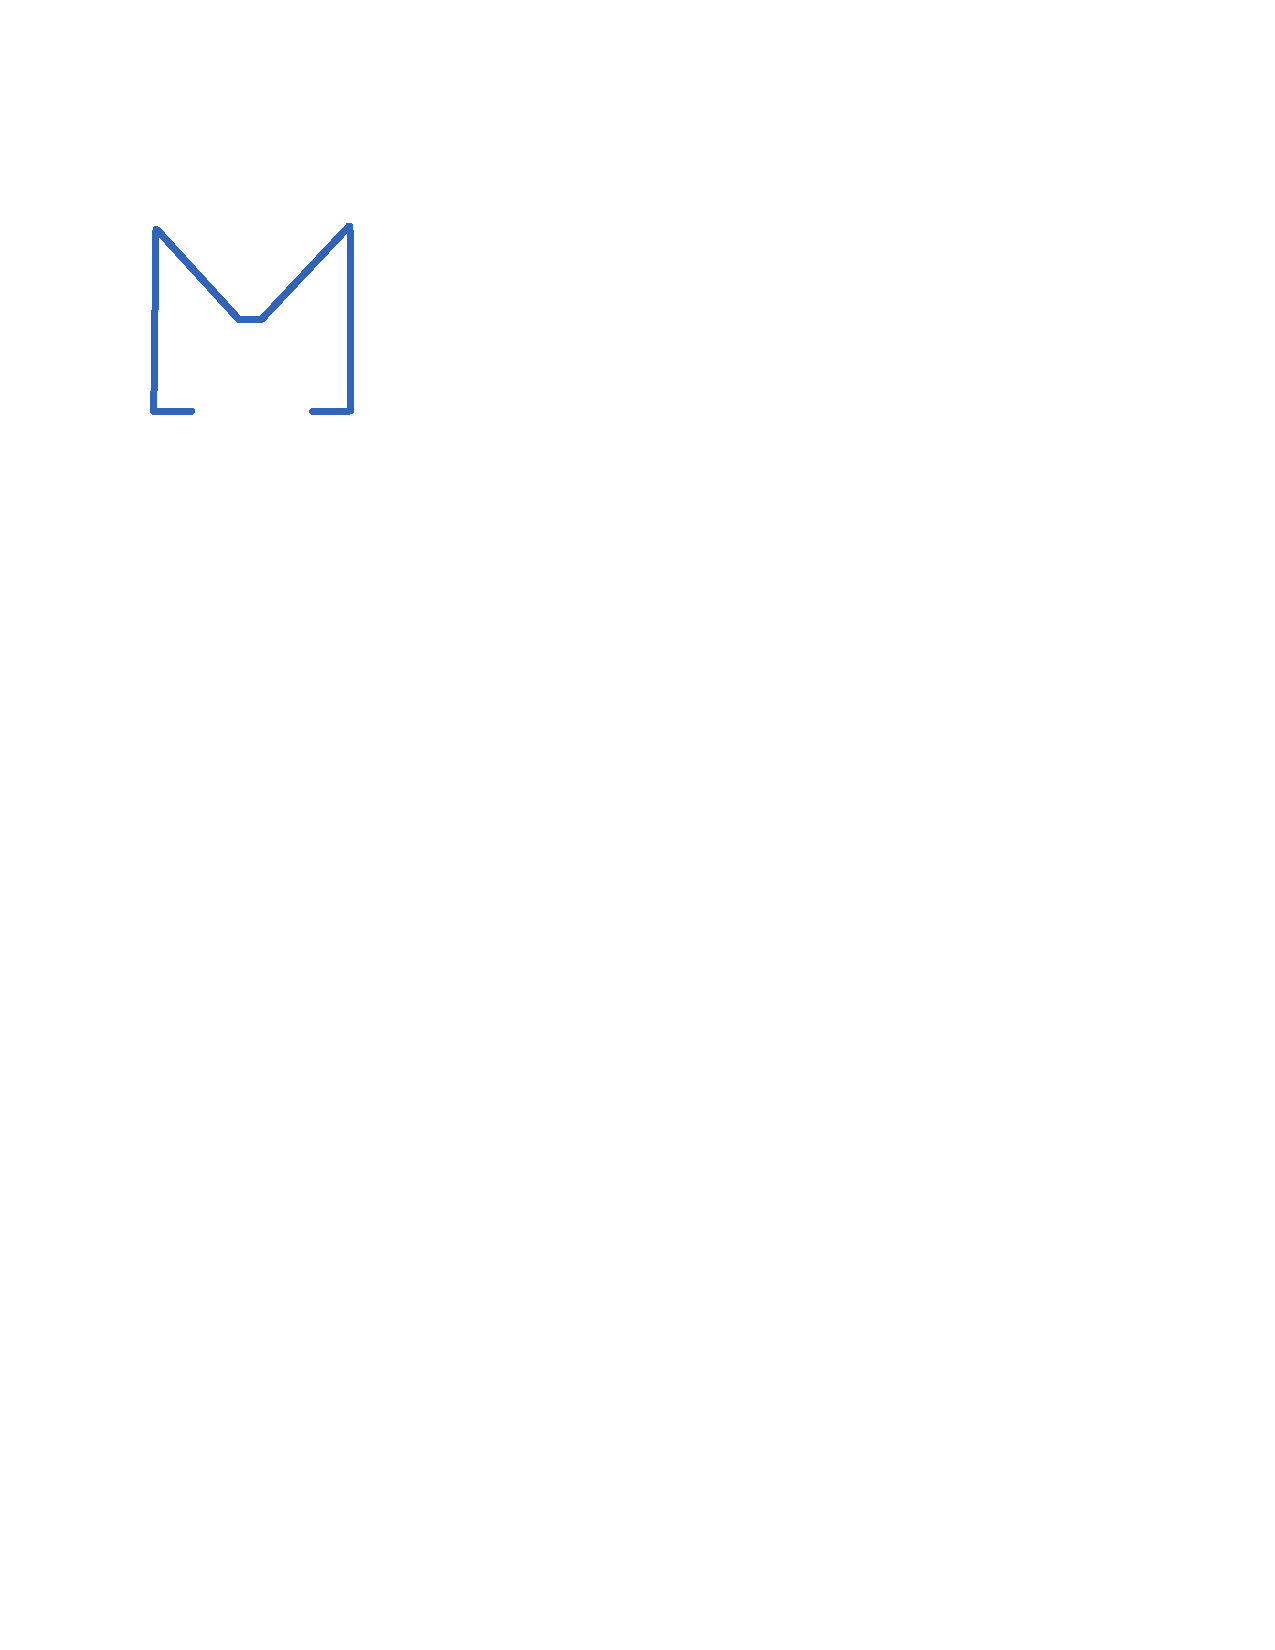
\includegraphics[scale=0.5]{M.pdf}
\end{center}

\begin{defn}
Let $[a,b]\subseteq \R$ be an interval, let $\{t_1,t_2,\cdots, t_n\}$ defines a partition of $[a,b]$. For piecewise function $\alpha:[a,b]\to \R^n$ that satisfies $\alpha|_{[t_{j-1},t_j]}$ being continuous on  $[t_{j-1},t_j]$, we denote $\alpha_{(j)} \coloneqq \alpha|_{[t_{j-1},t_j]}$.
\end{defn}

\begin{defn}
For $\alpha \in C_{pw}^k([a,b],\R^n)$, $Y \coloneqq \alpha([a,b])$ is usually denoted as $Y_{\alpha}$, and we write:
$$\int_{Y_{\alpha}} \omega = \int_{[a,b]} \alpha^*\omega$$
where $\omega $ is a $1$-form defined on $Y$. Moreover, for function $f$ such that $df$ is a $1$-form defined on $[a,b]$, we write the following:
$$\int_{Y_\alpha} df = \sum_j \int_{Y_{\alpha_{(j)}}}df = \sum_j \Delta_{Y_{\alpha_{(j)}}} f$$  
\end{defn}

\begin{thm}
Let $A$ be an open connected subset of $\R^n$, let $f \in C^1(A,\R)$. $df(x) = 0$ for $x \in A$ if and only if $f$ is a constant function. 
\end{thm}
\begin{proof}
The $\Leftarrow$ direction is trivial. For the $\Rightarrow$ direction, we know that open sets can be decomposed into path connected components, one can choose $\alpha\in C^1_{pw}$ such that $\Delta_{Y_\alpha} f = \int_{Y_\alpha} df = 0 \Rightarrow f(b) = f(a)$. This completes the proof of this theorem.
\end{proof}

\newpage
\section[Integration of One-forms]{\color{red}Integration of One-forms \color{black}}
We now have defined two kinds of integrals over a parametrized $k$-manifold $Y_\alpha$ in $\R^n$, with coordinate patch $\alpha$ defined on $I$, one for usual function $g$ and one for $1$-form $\omega$:
\begin{enumerate}[topsep=3pt,itemsep=-1ex,partopsep=1ex,parsep=1ex]
\item For function $g:Y\to \R$, we have $\int_{Y_\alpha} g\, dV = \int_I (g\circ \alpha)\mathcal{V}(D\alpha)$
\item For 1-form $\omega$ defined on $Y$, $\int_{Y_\alpha} \omega = \int_{I} \alpha^*\omega$
\end{enumerate}
If $I \subseteq \R$, then we can write the following:
$$\int_{Y_{\alpha}} g\, dV = \int_I (g\circ \alpha) \sqrt{\det((D\alpha)^TD\alpha)} = \int_I (g\circ \alpha) ||D\alpha|| = \int_I (g\circ \alpha) ||\alpha'||$$
On the other hand, we have:
$$\int_{Y_\alpha} (\omega \circ \alpha) \cdot D\alpha= \int_I (\omega \circ \alpha) \cdot \alpha'$$
Here we have $\int_{Y_\alpha} g\, dV  = \int_{Y_\alpha} \omega$ provided that we have the following holds:
$$(g\circ \alpha)||\alpha'|| = (\omega \circ \alpha) \alpha'$$
That is, for all $t\in I$, with $\vec{p} = \alpha(t)$, we must have $g(\vec{p})||\alpha'(t)|| = \omega(\vec{p})\cdot \alpha'(t)$, which is equivalent to the following:
$$g(\vec{p}) = \omega(\vec{p}) \cdot \frac{\alpha'(t)}{||\alpha'(t)||}$$
Here we require $\alpha'(t) \neq 0$ and $\alpha$ being injective. If $\alpha\in C^1$ is injective and $\alpha'(t)\neq 0$ for all $t \in I$, then one can set $T:Y \to \R^n \ \ \ \alpha(t)\mapsto \frac{\alpha'(t)}{||\alpha'(t)||}$, and get the followings:
$$\int_{Y_{\alpha}} (\omega \cdot T)dV = \int_{Y_\alpha}\omega \qquad\qquad\qquad\qquad\qquad\int_{Y_{\alpha}} g\, dV = \int_{Y_\alpha} (g\cdot T^T)$$
\hfill\break

\begin{thm}[Fundamental Theorem of Calculus I(a) for 1-forms]
Let $\omega$ be a 1-form on $A$, where $A$ is a connected open subset of $\R^m$. \\
The followings are equivalent:
\begin{enumerate}[topsep=3pt,itemsep=-1ex,partopsep=1ex,parsep=1ex]
\item $\omega = df$ for some $f \in C^1(A,\R)$, in which case $\omega$ is said to be exact on $A$.
\item For $\alpha \in C_{pw}^1 ([a,b],A)$ with $\alpha(a) = \alpha(b)$, we have $\int_{Y_\alpha} \omega = 0$.
\item For $\alpha_j \in C_{pw}^1 ([a_j,b_j],A)$ with $\alpha_1(a_1) = \alpha_2(a_2)$ and $\alpha_1(b_1) = \alpha_2(b_2)$, we have $\int_{Y_{\alpha_1}}\omega = \int_{Y_{\alpha_2}} \omega $, in which case $\omega$ is said to be path independent. 
\end{enumerate}
\end{thm}
\begin{proof}
First we note that (1) implies (2) is immediate by previous discussion: 
$$\int_{Y_\alpha} df = f(\alpha(b))-f(\alpha(a)) = 0$$
Details of (2) implying (3) can be found on Theorem M.1 on the Math 395 Supplement materials. The idea is reversing the orientation of $\alpha_2$ in (3) and form a closed loop to get $\int \omega = 0$. Now we will show (3) implies (1), for $a,b \in A$, one can define the integral $\int_a^b \omega$ with the path independent property of $\omega$ such that the following holds:
$$\int_x^y \omega + \int_y^z \omega = \int_x^z \omega$$
for $x,y,z \in A$. Fix $x_0 \in A$, define $f(x) = \int_{x_0}^ x \omega$, we will show that we have $df = \omega$ for some $f \in C^1(A,\R)$, that is, we want to evaluate the following as $h\in \R^m$ tends to zero:
\begin{align*}
\frac{f(x+h)-f(x) -\omega(x)\cdot h}{||h||} \tag{*}
\end{align*}
Assuming that $h$ is small enough, with $\alpha:[0,1]\to A\ \ \ t\mapsto x+th$ such that $\alpha'(t) = h$, we can write the following:
$$f(x+h)-f(x) = \int_x^{x+h}\omega = \int_0^1 \omega (x+th) \cdot h\, dt $$
So we can write:
\begin{align*}
(*) = \frac{\int_0^1 \left(\omega(x+th) - \omega(x)\right)\cdot h \, dt}{||h||}
\end{align*}
Here we see that:
$$|(*)|\leq \frac{\int_0^1||\omega(x+th)-\omega(x)||\cdot ||h||\, dt}{||h||} \leq \max_{0\leq t\leq 1} ||\omega(x+th)-\omega(x)||$$
It follows that $\lim_{h\to 0}(*) = 0$. The results of this theorem follows immediately.
\end{proof}

Let $\omega$ be a one form defined on an open subset $A$ of $\R^m$. By Corollary 6.2.1, the Clairaut's Theorem, suppose there exists $f \in C^2$ such that $D_jf = \omega_j$ and $D_kf = \omega_k$, here we have $D_kD_jf = D_jD_kf$, so if we have $\omega \in C^1$ and is exact, then $D_k\omega_j = D_j \omega_k$, in which case $\omega$ is said to be closed on $A$. 

\begin{defn}
Let $A$ be an open subset of $\R^m$, let $\omega$ be a $1$-form defined on $A$.\\
$\omega$ is said to be closed on $A$ provided that $D_k\omega_j = D_j \omega_k$. 
$\omega$ is said to be exact on $A$ provided that $\omega = df$ for some $f \in C^1(A,\R)$. $\omega$ is said to be path independent provided that $\int_{Y_{\alpha_1}} \omega = \int_{Y_{\alpha_2}}\omega$ for $\alpha_j \in C_{pw}^1([a_j,b_j],A)$ with $\alpha_1(a_1) = \alpha_2(a_2)$ and $\alpha_1(b_1) = \alpha_2(b_2)$. 
\end{defn}

\example Consider the $1$-form $\omega $ defined on $\R^2$ that maps $(x_1,x_2)$ to $(-\frac{x_2}{x_1^2+x_2^2} , \frac{x_1}{x_1^2+x_2^2})$.\\
One can verify that $\omega$ is closed on $\R^2 \setminus \{\vec{0}\}$ with $\omega = d(\arctan(\frac{x_2}{x_1}))$ on $(0,\infty) \times \R$.\\
For $\alpha:[0,2\pi] \to \R^2 \ \ \ t\mapsto (\cos(t),\sin(t))$, we can write the following:
\begin{align*}
\int_{Y_\alpha} \omega = \int_0^{2\pi} \alpha^*\omega &= \int_0^{2\pi} (-\sin(t))d(\cos(t)) + \cos(t) d(\sin(t)) \\&= \int_0^{2\pi} (-\sin(t))(-\sin(t))dt + \cos(t)\cos(t)dt \\&= \int_0^{2\pi} dt \\&= 2\pi \neq 0
\end{align*}
Here we conclude that $\omega$ is not exact on $\R^2 \setminus \{\vec{0}\}$. 
\newpage

\begin{lem}
Let $\omega$ be a closed 1-form of $C^1$ type, and let $\alpha$ be a $C^2$ type function. Then $\alpha^*\omega$ is closed. 
\end{lem}
\begin{proof}
Check Theorem 32.3 on Munkres and Lemma M.6 on Math 395 Supplement material.
\end{proof}

\begin{lem}[Green's Theorem for Two-dimensional Boxes]
Let $\omega$ be a 1-form defined on an open set $A\subseteq \R^2$ which contains a box $R$ of $\R^2$, then we have the following holds: 
$$\int_{\substack{{\Bd(R)}\\ \text{ counter-clockwise orientation}}} \omega = \int_R (D_1\omega_2 - D_2\omega_1)$$ 
where $\omega_1,\omega_2$ are component functions of $\omega$. The counter-clockwise orientation of $\Bd(R)$ refers to a path which maps an interval in $\R$ to $\Bd(R)$ that goes in counter-clockwise direction on $\Bd(R)$.
\end{lem}
\begin{proof}
Denote $a_1\leq x_1\leq b_1$, $a_2\leq x_2\leq b_2$. 
\begin{align*}
\int_{\Bd(R)}\omega =&+ \int_{a_1}^{b_1}\omega_1(x_1,a_2)\, dx_1+\int_{a_2}^{b_2}\omega_2(b_1,x_2)\, dx_2 \\
&-\int_{a_1}^{b_1} \omega_1 (x_1,b_2)dx_1 - \int_{a_2}^{b_2} \omega_2(a_1,x_2)dx_2\\
=& \int_{a_2}^{b_2}\int_{a_1}^{b_1} D_1\omega_2(x_1,x_2)\,dx_1\, dx_2 \ -\  \int_{a_1}^{b_1}\int_{a_2}^{b_2} D_2\omega_1(x_1,x_2)\,dx_2\,dx_1\\
=& \int_R (D_1\omega_2 - D_2\omega_1)
\end{align*}
The result of this lemma follows.
\end{proof}

\begin{corL}
Let $\omega$ be a 1-form on an open set containing a box $R$ of $\R^2$, if $\omega$ is closed, then we have: 
$$\int_{\Bd(R)}\omega = 0$$
\end{corL}


\begin{thm}[Fundamental Theorem of Calculus I(b) for 1-forms]
Let $\omega$ be a closed 1-form on $A\subseteq \R^m$. \\
If $A$ is a convex open subset of $\R^m$, then  $\omega$ is exact on $A$.  
\end{thm}
\begin{proof}
Theorem M.5 on the Math 395 Supplement material gives a proof to this theorem.
\end{proof}

\remark In the settings of Theorem 19.2, the result also holds when $A$ is $C^2$-diffeomorphic to a convex set. Suppose a set $A$ is $C^2$-diffeomorphic to a convex set $B$, let $\omega$ be a closed $1$-form defined on $A$. Suppose further that $\gamma$ defines a $C^2$-diffeomorphism from $B$ to $A$. Then by Lemma 19.1.1, we know that $\gamma^*\omega$ defined on $B$ is closed, and hence $\gamma^*\omega$ is exact on $B$. That is, there exists some $f \in C^1$ such that $\gamma^*\omega  = df$. Then we can write $\omega = (\gamma\circ \gamma^{-1})^*\omega  = {\gamma^{-1}}^*(\gamma^*\omega) = {\gamma^{-1}}^*(df) = d({\gamma^{-1}}^*f)$.\\

\example Consider the $1$-form $\omega $ defined on $\R^2$ that maps $(x_1,x_2)$ to $(-\frac{x_2}{x_1^2+x_2^2} , \frac{x_1}{x_1^2+x_2^2})$.\\
We see that such $1$-form is closed but not exact on $\R^2 \setminus \{\vec{0}\}$, hence it follows that $\R^2 \setminus \{\vec{0}\}$ is not diffeomorphic to any convex set. 


\newpage
\section[Integral Manifolds]{\color{red}Integral Manifolds \color{black}}
Let $\omega$ be a $1$-form defined on an open subset $A$ of $\R^n$. Here $\omega$ can be viewed as a function from $A$ to $(\R^n)^* = \hom(\R^n, \R)$. For $\vec{p}\in A$, we have $\omega(\vec{p}):\R^n \to \R$, and $\dim(\ker(\omega(\vec{p}))) = n-1$ or $n$. 
\begin{prop}
Let $A$ be an open subset of $\R^n$, and let $\omega$ be a $1$-form defined on $A$. \\
For $k$-manifold $M\subseteq A$, the followings are equivalent:
\begin{enumerate}[topsep=3pt,itemsep=-1ex,partopsep=1ex,parsep=1ex]
\item $\T_{\vec{p}}(M) \subseteq \ker(\omega(\vec{p}))$ for all $\vec{p}\in M$
\item $\alpha^*\omega = 0$ for all coordinate patches $\alpha$ for $M$
\item $\int_C \omega =0$ for all $1$-manifold $C\subseteq M$. 
\end{enumerate} 
\end{prop}
\begin{proof}
The proof of this proposition is given in Math 396 HW1. 
\end{proof}

\begin{defn}
Let $\omega$ be a $1$-form defined on an open subset $A$ of $\R^n$, for $k$-manifold $M \subseteq A$, $M$ is called an integral manifold for $\omega$ provided that $\int_C \omega =0$ for all $1$-manifold $C\subseteq M$. 
\end{defn}

\note Let $\omega$ be a $1$-form defined on an open subset $A$ of $\R^n$. Integral manifolds for $\omega$ are also integral manifold for $g\omega$ where $g$ is a scalar function, because $\alpha^*(g\omega) = (\alpha^*g)(\alpha^*\omega)$.

\begin{lem}
Let $f \in C^1(A,\R)$ where $A$ is an open subset of $\R^n$, with $df \neq 0$ on $A$. \\Then, for $c \in \R$, the level set $f^{-1}(c)$ is an $(n-1)$-manifold without boundary.
\end{lem}
\begin{proof}
The proof of this lemma is given in Theorem I.6 on Math 396 Supplement Materials. 
\end{proof}

\begin{corL}
Let $f \in C^1(A,\R)$ where $A$ is an open subset of $\R^n$, with $df \neq 0$ on $A$.\\
Each level set of $f$ is an integral manifold for $df$.
\end{corL}
\begin{proof}
For some $c \in \R$, the level set $M \coloneqq f^{-1}(c)$ is an $(n-1)$-manifold without boundary. let $\alpha$ be a coordinate patch for $M$, we see that $\alpha^*(df) = d(\alpha^* f) = d(f\circ \alpha) = 0$, and here we have $f\circ \alpha = c$, hence $d(f\circ \alpha) = 0$, so $M$ is an integral manifold for $df$. 
\end{proof}

\subsection*{Integral curves for solving differential equations}
In this section, a function $f$ denoted as $f(x)$ has domain being a subset of $\R$ and codomain being a subset of $\R$; A function $g$ denoted as $g(x,y)$ has domain being a subset of $\R^2$ and codomain being a subset of $\R$. A $1$-form $\omega$ has domain $\R^2$ and codomain $\R^2_{row}$.\\

Let $\omega = U(x,y)\, dx + V(x,y) \, dy$ be defined on an open subset $A$ of $\R^2$, with $V$ being a non-vanishing function on $A$. Let $f \in C^1((a,b),\R)$. Consider a parametrized manifold $M\coloneqq Graph(f) \subseteq A$ parametrized by $\alpha:(a,b) \to M \ \ \ x\mapsto (x,f(x))$ for some continuous function $f:\R \to \R$. Here we observe that $M$ is an integral manifold for $\omega$ if and only if $\alpha^* \omega = 0$, where we have:
$$\alpha^*\omega = (U(x,f(x))+V(x,f(x))f'(x)) =0 \quad \iff \quad f'(x) =- \frac{U(x,f(x))}{V(x,f(x))}$$ 
Suppose further that $U,V \in C^1(\R^2,\R)$, then $-\frac{U(x,y)}{V(x,y)} \in C^1$, consider $(0,y_0) \in A$, we claim that there exists $\Phi \in C^1(\R^2,\R)$ with bounded function $D\Phi :\R^2 \to \R^2_{row}$ such that $\Phi (x,y) = -\frac{U(x,y)}{V(x,y)}$ for $(x,y)$ in the neighborhood of the point $(0,y_0)$. Here we will prove the claim:
\begin{proof}
Pick $\eta \in C^\infty (\R^2, \R)$ with $\eta(x,y) = 1$ in neighborhood of $(0,y_0)$ such that $supp(\eta)$ is a compact subset of $A$. Then we define the following:
$$\Phi(x,y) = \begin{cases}-\frac{U(x,y)}{V(x,y)}\eta(x,y) & (x,y) \in A \\ 0 &(x,y) \notin A \end{cases}$$
Here $D\Phi$ is bounded because $\Phi$ has compact support, and $\Phi$ satisfies the conditions in the claim. This completes the proof.
\end{proof}
By Math 395 HW4 Q6, $\Phi$ is partially Lipschitz on $\R^2$. By Math 395 HW10 Q5, $\exists\ \epsilon>0$ such that $f'(x) = \Phi(x,f(x))$ has a unique solution $f$ on $(-\epsilon,\epsilon)$. One can shrink $\epsilon$, if necessary, to $\bar{\epsilon}>0$ such that $f'(x) = -\frac{U(x,f(x))}{V(x,f(x))}$ has unique solution $f$ on $(-\bar{\epsilon},\bar{\epsilon})$, so there exists a unique local integral curve for $\omega$ passing through $(0,y_0)$. We claim that we get the same result for each $(x_0,y_0) \in A$, one can show by using a translation in the $x$-direction. \\

If $U$ and $V$ are continuous but not differentiable, one can show that the solutions guaranteed to exist, but the uniqueness can fail. One example is given by Math 395 HW11 Q5, which considers the $1$-form $\omega = y^{1/3}\,dx - dy$ with $f'(x) = \sqrt[3]{f(x)}$\\

Conversely given differential equation: 
\begin{align*}
f'(x) = \Phi(x,f(x)) \tag{D1}
\end{align*}
then the graphs of solutions of (D1) are integral curves for $\omega \coloneqq -\Phi(x,y)dx+dy$, and also for $\that{\omega} \coloneqq B(x,y) \omega = -B(x,y)\Phi(x,y)\, dx + B(x,y)\, dy$ with some function $B(x,y)$. If $\that{\omega}$ is exact, that is, if $\that{\omega} = dg$ for some function $g$, then $B$ is called an integrating factor for $\omega$. For constant $c$, since the level set $g^{-1}(c)$ is integral manifolds for $dg = \that{\omega}$, assuming $B$ is not the zero function, then $g^{-1}(c)$ is also an integral manifold for $\omega = \Phi(x,y)\, dx + dy$, and hence $g^{-1}(c)$ is a graph of solutions of (D1).\\

Now suppose $f$ solves the differential equation (D1), then we can write the following:
\begin{align*}
\frac{d}{dx} \left( g\bmat{x \\ f(x)}\right) &= dg\left(\bmat{x\\ f(x)}\right) \cdot \bmat{1 \\ f'(x)} \\
&= \bmat{-B\left(\bmat{x \\ f(x)} \right)\Phi\left(\bmat{x \\ f(x)} \right) & B\left(\bmat{x \\ f(x)} \right)} \cdot \bmat{1 \\ f'(x)} \\
&= -B\left(\bmat{x\\ f(x)}\right) \Phi\left( \bmat{x\\f(x)}\right) + B\left( \bmat{x\\ f(x)}\right) f'(x) = 0
\end{align*}
Here we see that $g(x,f(x))$ is locally constant on each component of domain of definition for $g(x,f(x))$. In conclusion, the good news are, such $B$ always exists, looking for $B$ is often useful when solving differential equation (D1), but the bad news is that finding such $B$ is not always easier than trying to solve (D1). \\
\newpage

Here are two classes of examples:
\begin{enumerate}
\item Consider $f'(x) = \beta(f(x))$, that is, here we suppose the velocity of a particle is given by the predetermined function of its position, and the position function $f(x)$ of the particle is a function of time $x$. Here we want $-B(x,y) \beta(y)\, dx + B(x,y)\, dy$ to be exact with some integrating factor $B(x,y)$, one can choose $B(x,y) = \frac{1}{\beta (y)}$. Then the solution to  $f'(x) = \beta(f(x))$ are integration curves for the $1$-form: $$-dx + \frac{dy}{\beta(y)} = d\left(-x + \int \frac{dy}{\beta(y)}\right)$$ Hence the solutions $f(x)$ for the differential equation $f'(x) = \beta(f(x))$ satisfies $-x + \int \frac{dy}{\beta(y)} = C$. Solving $y = f(x)$ could be done implicitly. In the following, we will try to calculate the travel time from position $y_0$ to $y_1$. the path is traced out by the parametrized manifold $M$: 
\begin{center}
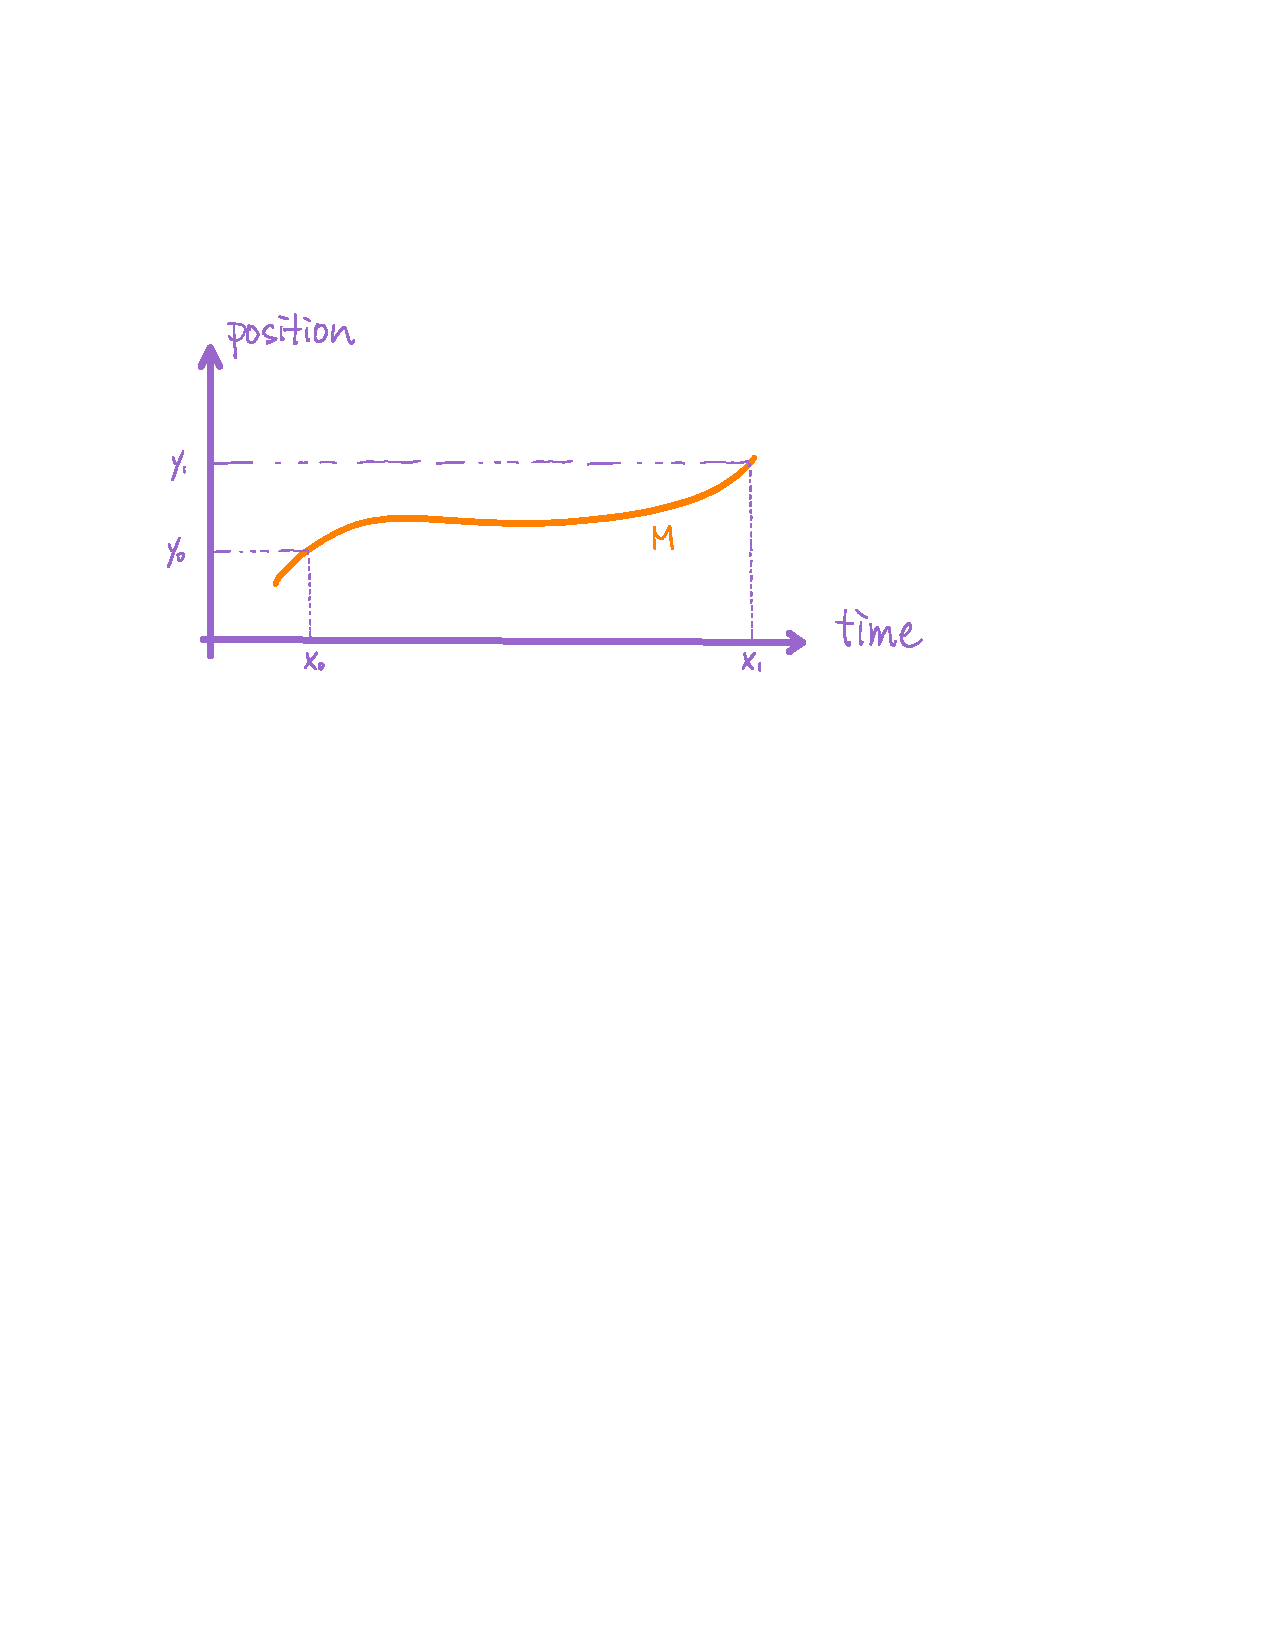
\includegraphics[scale=0.7]{integralCurve.pdf}
\end{center}
\begin{align*}
x_1 - x_1 = \int_M dx = \int_M dx + \int_M \left( -dx + \frac{dy}{\beta(y)}\right) = \int_M \frac{dy}{\beta(y)} = \int_{y_0}^{y_1}\frac{dy}{\beta(y)}
\end{align*}
\item Consider $f''(t) = \beta(f(t))$ with $f(t_0) = x_0$ and $f'(t_0) = x_1$, that is, here we suppose we have a unit mass particle in 1-dimensional universe, subject to force field $\beta (x)$. Let $h(t) = f'(t)$, and let $h'(t) = \beta(f(t)) = f''(t)$. Then we can write the following:
$$ \bmat{f(t_0)\\ h(t_0)} = \bmat{x_0\\x_1}$$
with the following:
\begin{align*}
\bmat{f'(t) \\ h'(t)} = \bmat{h(t) \\ \beta(f(t))} \coloneqq \Psi\bmat{f(t) \\ h(t)} \qquad\Rightarrow \qquad \bmat{f'\\ h'} = \Psi \circ \bmat{f \\ h} \tag{D2}
\end{align*}
Math 395 HW10 Q6 suggests that there is a unique local solution $(f,h)$ for such $\Psi$ if $\beta\in C^1$. Suppose $f$ and $h$ solves the system (D2). Consider $\alpha: x\mapsto (x, f(x), h(x))$, and consider the manifold $Y_\alpha$ parametrized by $\alpha$. Denote $(t,x,v) \in \R^3$, we have $x= f(t), \ v=h(t) = f'(t)$ for $(t,x,v) \in Y_{\alpha}$. Here we see that $Y_\alpha$ is a integral manifold for $\omega_1 = dx - h\,dt$, and also for $\omega_2 = dv -\beta\, dt$, where $\omega_1$ and $\omega_2$ are not closed, hence not exact. One can show that $\omega_1$ has no integral $2$-manifold, and $\omega_1$ has no non-zero integrating factors. \\

\exercise If $M$ is a integral manifold for the $1$-form $\omega_1$ and for the $1$-form $\omega_2$, then $M$ is integral for the $1$-form $f_1 \omega_1 + f_2 \omega_2$, where $f_1$ and $f_2$ are scalar functions.  \\

Applying to specific situation, $\omega_3 \coloneqq h\cdot\omega_2 - \beta\cdot \omega_1 = h\,dv - \beta \, dx = d(\frac{h^2}{2} - \int \beta \, dx)$. Note that $\beta$ is a function of $x$ for $(t,x,v) \in Y_{\alpha}$. Hence $\frac{h^2}{2} - \int \beta \, dx$ is constant for any solution of the system (D2). In physics interpretation, at any point $(t,x,v) \in Y_{\alpha}$, $\frac{(h(t))^2}{2} =\frac{(f'(t))^2}{2} =  \frac{v^2}{2}$ is the kinetic energy of an object of unit mass, and $-\int \beta dx$ is the potential energy. 
\begin{align*}
E \coloneqq \frac{h^2}{2} - \int \beta \, dx
\tag{E}
\end{align*}
here $E$ gives the total energy of the system, which is a constant. Also $\beta$ can be interpreted as a function of $\text{force field}$ divided by the ${\text{constant mass}}$ of a particle, and the path of the particle is traced out by $f(t)$ as a function of time $t$. Rearranging equation (E) we can write:
$$f'(t) = \pm \sqrt{2\left(E+\int \beta\, dx\right)} $$
which is a autonomous first order equation, and by the first class of example in this section, one can get the following implicit solution to the system (D2):
$$t+C = \pm \int \frac{dx}{\sqrt{2(E+\int \beta \, dx)}}$$
with $x = f(t)$, and some constant $C$ determined by the initial conditions. \\

\example (Simple Harmonic Motion) Take $\beta(x) = -x$. \\
We get $E = \frac{v^2 + x^2}{2}$, and we have: $$t+C = \pm \int \frac{dx}{\sqrt{2E-x^2}} = \pm \arcsin\left(\frac{x}{\sqrt{2E}}\right) \qquad\Rightarrow\qquad x = \sqrt{2E} \sin(t+C)$$ which is called a simple harmonic motion of a particle. \\

\example (The Motion of a Frictionless Pendulum) Take $\beta(x) = -\sin(x)$. 
\\We get $E = \frac{v^2}{2}-\cos(x)$, hence $v^2 = 2(E+\cos(x))$, so $v = \pm \sqrt{2(E+\cos(x))}$.
$$t+C = \pm \int \frac{dx}{\sqrt{2(E+\cos(x)}} = \pm \frac{\sqrt{2}\cdot  \textit{Elliptic\,F}\left[ \frac{x}{2}, \frac{2}{1+E}\right]}{\sqrt{1+E}}$$\\

\example (The Motion of a Pendulum under Friction) \\Take $f''(t) = -\sin(f(t)) -\gamma \cdot f'(t)$ for some constant $\gamma$. \\
One can show that $E'(x) <0$. 
\end{enumerate}


\newpage
\chapter{Complex Analysis \ \rom{1}}
\setcounter{section}{20}
\section[Integration of Complex-valued Functions]{\color{red}Integration of Complex-valued Functions\color{black}}
\begin{defn}
Let $A$ be an open subset of $\R^n$, let $f:A \to \Complex$ be a function, with $u:A \to \R\ \ \ \vec{a}\mapsto \Re(f(\vec{a}))$ and  $v:A\to \R \ \ \ \vec{a}\mapsto \Im(f(\vec{a}))$, the integral of $f$ over $A$ is defined to be the following:
\begin{align*}
\int_A f \coloneqq \int_A u + i\, \int_A v
\end{align*}
here extended integral can be used when $\int_A u_+$, $\int_A u_-$, $\int_A v_+$, and $\int_A v_-$ are all finite. 
\end{defn}

\note Let $A$ be an open subset of $\R^n$, let $f:A \to \Complex$ be a function, we write $f = u + iv$ for functions $u$ and $v$ provided that $u$ and $v$ are real-valued, and they are characterized by $u:A \to \R\ \ \ \vec{a}\mapsto \Re(f(\vec{a}))$ and  $v:A\to \R \ \ \ \vec{a}\mapsto \Im(f(\vec{a}))$. 

\begin{defn}
Let $A$ be an open subset of $\R^n$, let $f:A \to \Complex  \ \ \ \vec{a}\mapsto f(\vec{a})$ with $f = u+iv$. \\
For parametrized manifold $Y_\alpha \subseteq A$, we define the following:
\begin{align*}
\int_{Y_\alpha} f\, dV = \int_{Y_\alpha}u \, dV + i \int_{Y_\alpha} v \, dV
\end{align*}
\end{defn}

\exercise Let $A$ be an open subset of $\R^n$, let $f:A \to \Complex$. For $\lambda \in \Complex$, we have: $$\int_A \lambda f = \lambda \int_A f$$


\begin{prop}
Let $A$ be an open subset of $\R^n$, let $f:A \to \Complex$.
$$\left|\int_A f\right| \leq \int_A |f|$$
\end{prop}
\begin{proof}
Note that $|\int_A f|\in \Complex$, and hence $|\int_A f| = e^{i\Phi} \cdot \int_A f$ for some $\Phi \in \R$. \\Then we obtain:
\begin{align*}
\left| \int_A f\right| = e^{i\Phi} \int_A f = \int_A e^{i\Phi} f
\end{align*}
Here $\int_A e^{i\Phi} f \in \R$. That is, if we write $v:A \to \R \ \ \ \vec{a}\mapsto \Im(f(\vec{a}))$, then $i \int_A v = 0$. \\Then we obtain the following by the triangle inequality:
$$\int_A e^{i\Phi} f = \int_A \Re(e^{i\Phi} f) \leq \int_A |e^{i\Phi} f| = \int_A |e^{i\Phi}| \cdot |f| = \int_A |f|$$
This completes the proof.
\end{proof}


\newpage
\section[Holomorphic Functions]{\color{red}Holomorphic Functions\color{black}}
\begin{defn}
Let $A$ be an open subset of $\R^n$, $\omega:A \to \Complex^n_{row}$ is called a $\Complex$-valued $1$-form. Denote $\omega = \omega_1 + i \omega_2$,  where $\omega_1: A \to \R^n_{row} \ \ \ \vec{a}\mapsto \Re(\omega(\vec{a}))$ and $\omega_2:A \to \R^n_{row}\ \ \ \vec{a}\mapsto \Im(\omega(\vec{a}))$, and let $Y_\alpha \subseteq A$ be a parametrized manifold, we define: 
$$\int_{Y_\alpha} \omega \coloneqq \left(\int_{Y_\alpha} \omega_1 \right)+\left( i\int_{Y_\alpha} \omega_2\right)$$
\end{defn}

\exercise In the settings of Definition 21.0.1.0.1, we get $\int_{Y_\alpha} \lambda \omega = \lambda \int_{Y_\alpha} \omega$ for $\lambda \in \Complex$. \\
If $Y_\alpha$ is a parametrized $1$-manifold, we get the following:
$$\left| \int_{Y_\alpha}  \omega \right| \leq (\text{The length of }Y_\alpha) \cdot \sup_{\vec{x}\in Y} ||\omega (\vec{x})||$$


\begin{defn}
Let $A$ be an open subset of $\R^n$, let $f:A \to \Complex$ with $f = u+iv$ for functions $u$ and $v$. The function $f$ is said to be of $C^r$ type, denoted as $f \in C^r(A,\Complex)$, provided that $u,v \in C^r(A,\R)$. Here we define $D_j f \coloneqq D_j u + i D_j v$ if $f \in C^1(A,\Complex)$ is given. 
\end{defn}


\note Let $A$ be an open subset of $\R^n$, let $f:A \to \Complex$ with $f=u+iv$, we have: $$df = du + i dv$$ 
\note Consider $z:\R^2 \to \Complex \ \ \ (x,y)\mapsto x+iy$,\footnote{In this chapter, Complex Analysis I, and the chapter Complex Analysis II, if not specified, one might consider the notation $z$ is referred to the function $z:\R^2 \to \Complex \ \ \ (x,y)\mapsto x+iy$, where we denote $z = x+iy$} we write $\bar{z}:\R^2 \to \Complex \ \ \ (x,y) \mapsto x-iy$, and we get the following:
$$dz = dx+idy \qquad\qquad\qquad d\bar{z} = dx - i dy$$ 
Rearranging we have:
$$dx = \frac{dz+d\bar{z}}{2}\qquad\qquad\qquad dy = \frac{dz-d\bar{z}}{2i}$$

\subsection*{Euler's Formula}
With $dz = dx+idy$, we proceed to investigate the $1$-form $\frac{dz}{z}$ defined on $\Complex\setminus \{0\}$.
\begin{align*}
\frac{dz}{z} &= \frac{dx+i dy}{x+iy}\\
&= \frac{x-iy}{x-iy}\cdot \frac{dx + iy}{x+iy}\\
&= \left( \frac{x\, dx}{x^2+y^2} + \frac{y\, dy}{x^2+y^2}\right) +i\left(-\frac{y\, dx}{x^2+y^2} dx + \frac{x\, dy}{x^2+y^2}\right) \tag{*}
\end{align*}
Let $\log$ function defined by the followings:
$$\log: (0,\infty) \to \R \ \ \ \ m \mapsto \int_1^m \frac{1}{t}$$
Let $X\subseteq \Complex$ be a ray starting at $\vec{0}$ making an angle $\theta_0 = 0$ from the $x$-axis.\\ One can define polar coordinates $(r,\Phi_X)$ on $\Complex \setminus X$ with $0< \Phi_X < 2\pi$:
$$r:\Complex \setminus X\to \R \ \ \ z\mapsto \sqrt{(\Re(z))^2 + (\Im(z))^2}$$
$$\Phi_X: \Complex\setminus X \to (0,2\pi) \ \ \ z\mapsto \cos^{-1}\left(\frac{\Re{(z)}}{\sqrt{(\Re{(z)})^2+(\Im(z))^2}}\right)$$ 
In general, one can propose a definition for the polar coordinate $(r,\Phi_X)$ on $\Complex \setminus X$, with $X$ being a ray starting at $\vec{0}\in \Complex$ making an angle $\theta_0 \in \R$ from the $x$-axis, in which case the codomain of $\Phi_X$ is defined to be on $(\theta_0,\, \theta_0 + 2\pi)$. \\

For nonzero $z\in \Complex$, the polar coordinate of $z$ is denoted as $(r(z),\Phi_X(z))$. Here $r(z)$ is called the absolute value, or the modulus, of $z$, and $\Phi_X(z)$ is called the argument, or phase, of $z$. Here we denote $|z| \coloneqq r(z)$, and $\text{arg}(z) \coloneqq \Phi_X(z)$. \\


One can show that the equation (*) is exact on $\Complex \setminus X$.\\
Equation (*) suggests that we can define the following:
$$\log_X:\Complex\setminus X \to \Complex \ \ \ \omega \mapsto \int_1^\omega \frac{dz}{z} = \int_1^\omega d\log(r) + i\, d\Phi_X = \log (r(\omega)) + i\,\Phi_X(\omega)$$ 


Solve $z = \log_X \omega$ for $\omega \in \Complex$, we get $\Re(z) = \log r(\omega)$ and $\Im(z) = \Phi_X(\omega)$, so we can write:
$$e^z \coloneqq \omega = r(\omega)(\cos(\Phi_X(\omega)) + i\sin(\Phi_X(\omega))) = e^{\Re(z)} (\cos(\Im(z))+ i\sin(\Im(z)))$$
Here $e^z = e^{\Re(z)} (\cos(\Im(z))+ i\sin(\Im(z)))$ is known as the Euler's Formula.\\






For $z=x+iy$, we also have the following holds:
\begin{align*}
de^z &= de^{x+iy}\\
&= d(e^x(\cos(y)+i\sin(y))) \\
&= e^x(\cos(y)+i\sin(y))dx + e^x(-\sin(y)+i\cos(y))dy \\
&= e^x(\cos(y) + i\sin(y)) (dx+idy)\\
&= e^z dz
\end{align*}

Let $A$ be an open subset of $\Complex$, let $f:A \to \Complex$ with $f = u+iv$ for functions $u$ and $v$.\footnote{Hereafter, we consider $\Complex \cong \R^2$ when defining a function $f:\Complex\to\Complex$, with $f=u+iv$, in which case it makes sense to write $D_1u$, $D_2u$, $D_1v$, and $D_2 v$. That is, $D_1u$ is the derivative of $u$ with respect to the real part of the input, and $D_2u$ is the derivative of $u$ with respect to the complex part of the input.} We can write:
$$f\, dz = (u+iv)(dx+idy) = (u+iv)dx+(iu-v) dy$$
If the $1$-form $f\, dz$ is closed, we need $D_1(if) = D_2(f)$. \\
Or equivalently, we need the following holds:
\begin{align*}
\begin{cases}
D_1 u = D_2 v\\
D_2 u = -D_1 v
\end{cases}
\tag{CR}
\end{align*}
The system (CR) of equations is called the Cauchy-Riemann Equations.

\begin{defn}
Let $A$ be an open subset of $\Complex$, a function $f:A \to \Complex$ of $C^1$ type, with $f = u+iv$, is holomorphic provided that $f\, dz$ is closed. Or equivalently, $f$ is holomorphic provided that the Cauchy-Riemann Equations hold for the function $f$. 
\end{defn}


\begin{thm}
Let $f$ be a holomorphic function defined on an open subset $A$ of $\Complex$. \\
If $A$ is diffeomorphic to a convex set, then $f\, dz$ is exact.
\end{thm}
\begin{proof}
The proof of this theorem follows similarly from M.8 in Math 396 Supplement Materials.
\end{proof}

\begin{corT}[Cauchy Integral Theorem]
Given a holomorphic function $f$ defined on an open subset $A$ of $\Complex$, where $A$ is diffeomorphic to a convex set, and given $\alpha:[a,b] \to A$ being a piecewise $C^1$ function with $\alpha(a) = \alpha(b)$, we have: $$\int_{Y_\alpha} f\, dz = 0$$
\end{corT}


\hfill\break

\example
Let $A$ be an open subset of $\Complex$, the followings are holomorphic functions:
\begin{enumerate}[topsep=3pt,itemsep=-1ex,partopsep=1ex,parsep=1ex]
\item $f:A \to \Complex  \quad z\mapsto z$
\item $f:A \to \Complex  \quad z\mapsto \log_X z$
\item $f:A \to \Complex  \quad z\mapsto c$ with $c \in \Complex$
\item $f:A \to \Complex  \quad z\mapsto z^{-1}$, that is, we have $f(x+iy) = \frac{x}{x^2 + y^2}-i\frac{y}{x^2 + y^2}$
\item $f:A \to \Complex  \quad z\mapsto e^z$, that is, we have $f(x+iy) = e^x \cos(y) + ie^x \sin(y)$
\end{enumerate}

\example
Let $A$ be an open subset of $\Complex$, the followings are non-holomorphic functions:
\begin{enumerate}[topsep=3pt,itemsep=-1ex,partopsep=1ex,parsep=1ex]
\item $f:A \to \Complex  \quad z\mapsto \bar{z}$, that is, we have $f(x+iy) = x-iy$
\item $f:A \to \Complex  \quad z\mapsto  \Re(z)$, that is, we have $f(x+iy) = x$
\item $f:A \to \Complex  \quad z\mapsto  \Im(z)$, that is, we have $f(x+iy) = y$\\
\end{enumerate}

\exercise Let $f$ and $g$ be holomorphic functions defined on an open subset $A$ of $\Complex$. \\
Then $f+g$, $f-g$ are holomorphic functions on $A$\\

\hfill\break
\begin{lem}
Let $f$ and $g$ be holomorphic functions defined on an open subset $A$ of $\Complex$. \\
Then $f\cdot g$ is ha holomorphic function on $A$.
\end{lem}
\begin{proof}
\begin{align*}
D_2(f\cdot g) = fD_2 g + gD_2 f = ifD_1 g+ igD_1 f = i(D_1(f\cdot g))
\end{align*}
The result follows.
\end{proof}

\newpage
\begin{lem}
Let $f$ and $g$ be holomorphic functions such that $g\circ f$ is well defined.\\ 
Then $g\circ f$ is a holomorphic function.
\end{lem}
\begin{proof}
For $z \in \Complex$, Cauchy-Riemann Equations require the followings hold:
\begin{align*}
D\bmat{\Re(f)(z) \\ \Im(f)(z)} = \bmat{\alpha &-\beta \\ \beta & \alpha} \qquad\qquad\qquad 
D\bmat{\Re(g)(z) \\ \Im(g)(z)} = \bmat{\gamma &-\delta \\ \delta & \gamma}
\end{align*}
for some scalars $\alpha,\beta,\gamma,\delta$. Here we get:
\begin{align*}
D\bmat{\Re(g\circ f)(z) \\ \Im(g\circ f)(z)} = \bmat{\gamma &-\delta \\ \delta & \gamma} \cdot \bmat{\alpha &-\beta \\ \beta & \alpha}  = \bmat{\sigma & -\tau \\ \tau & \sigma}
\end{align*}
for some scalars $\sigma,\tau$. The result follows.
\end{proof}

\begin{lem}
Let $f$ and $g$ be holomorphic functions defined on an open subset $A$ of $\Complex$, with $g\neq 0$. \\
Then $\frac{1}{g}$ and $\frac{f}{g}$ are holomorphic functions on $A$.
\end{lem}

\begin{corL}
The rational functions $\frac{P(z)}{Q(z)}$ are holomorphic on where defined. \\
Here $P(z)$ and $Q(z)$ are polynomial functions.
\end{corL}

\example \\
The function $f:\Complex \to \Complex  \quad z\mapsto e^{-z^2}$ is holomorphic on $\Complex$.\\
The function $f:\Complex \setminus \{\vec{0}\} \to \Complex  \quad z\mapsto \frac{e^{iz} -1}{z^2}$ is holomorphic on $\Complex \setminus \{\vec{0}\}$. 

\begin{prop}
Let $A,B$ be open subsets of $\Complex$. If the function $f:A \to B$ is a holomorphic diffeomorphism. Then the function $f^{-1}$ is holomorphic.
\end{prop}
\begin{proof}
Let $g\coloneqq f^{-1}$, by Cauchy-Riemann Equation, we can write:
\begin{align*}
D\bmat{\Re(f(z))\\ \Im(f(z))} = \bmat{\alpha & -\beta \\ \beta &-\alpha}
\end{align*}
with the following holds:
\begin{align*}
D\bmat{\Re(g(f(z)))\\ \Im(g(f(z)))} = \bmat{\alpha & -\beta \\ \beta &\alpha^{-1}}^{-1} = \bmat{\frac{\alpha}{\alpha^2+\beta^2}& \frac{\beta}{\alpha^2+\beta^2} \\ \frac{-\beta}{\alpha^2+\beta^2} & \frac{\alpha}{\alpha^2+\beta^2}}
\end{align*}
which agrees with the form required by Cauchy-Riemann Equations. The result follows.
\end{proof}

\newpage
\example Note that we have the following:
\begin{align*}
ext \int_{(x,y) \in \R^2}e^{-x^2 - y^2} = \int_{(x,y) \in \R^2}e^{-x^2}e^{-y^2} = \int_{y \in \R} e^{-y^2} \left(\int_{x \in \R} e^{-x^2} \right) = \left(\int_{x \in \R} e^{-x^2}\right)^2
\end{align*}
Or we can apply the Change of Variable Theorem:
\begin{align*}
ext \int_{(x,y) \in \R^2}e^{-x^2 - y^2} &= \int_{\R^2\setminus \{(x,0) \mid x\leq 0\}} e^{-x^2-y^2}\\
&= \int_{0}^\infty \int_{-\pi}^{\pi} e^{-r^2} r\, d\Phi dr \\
&= 2\pi \int_{0}^{\infty} e^{-r^2} r\, dr \\
&= \pi \int_{0}^\infty e^{-u} du \\
&= \pi
\end{align*}
So we see that we have:
\begin{align*}
\int_{x \in \R} e^{-x^2} = \sqrt{\pi}
\end{align*}

\hfill\break
\hfill\break
\example Consider the closed $1$-form $e^{-z^2} dz$ on $\Complex$ and the parametrized $1$-manifold given by the following:\\
\begin{center}
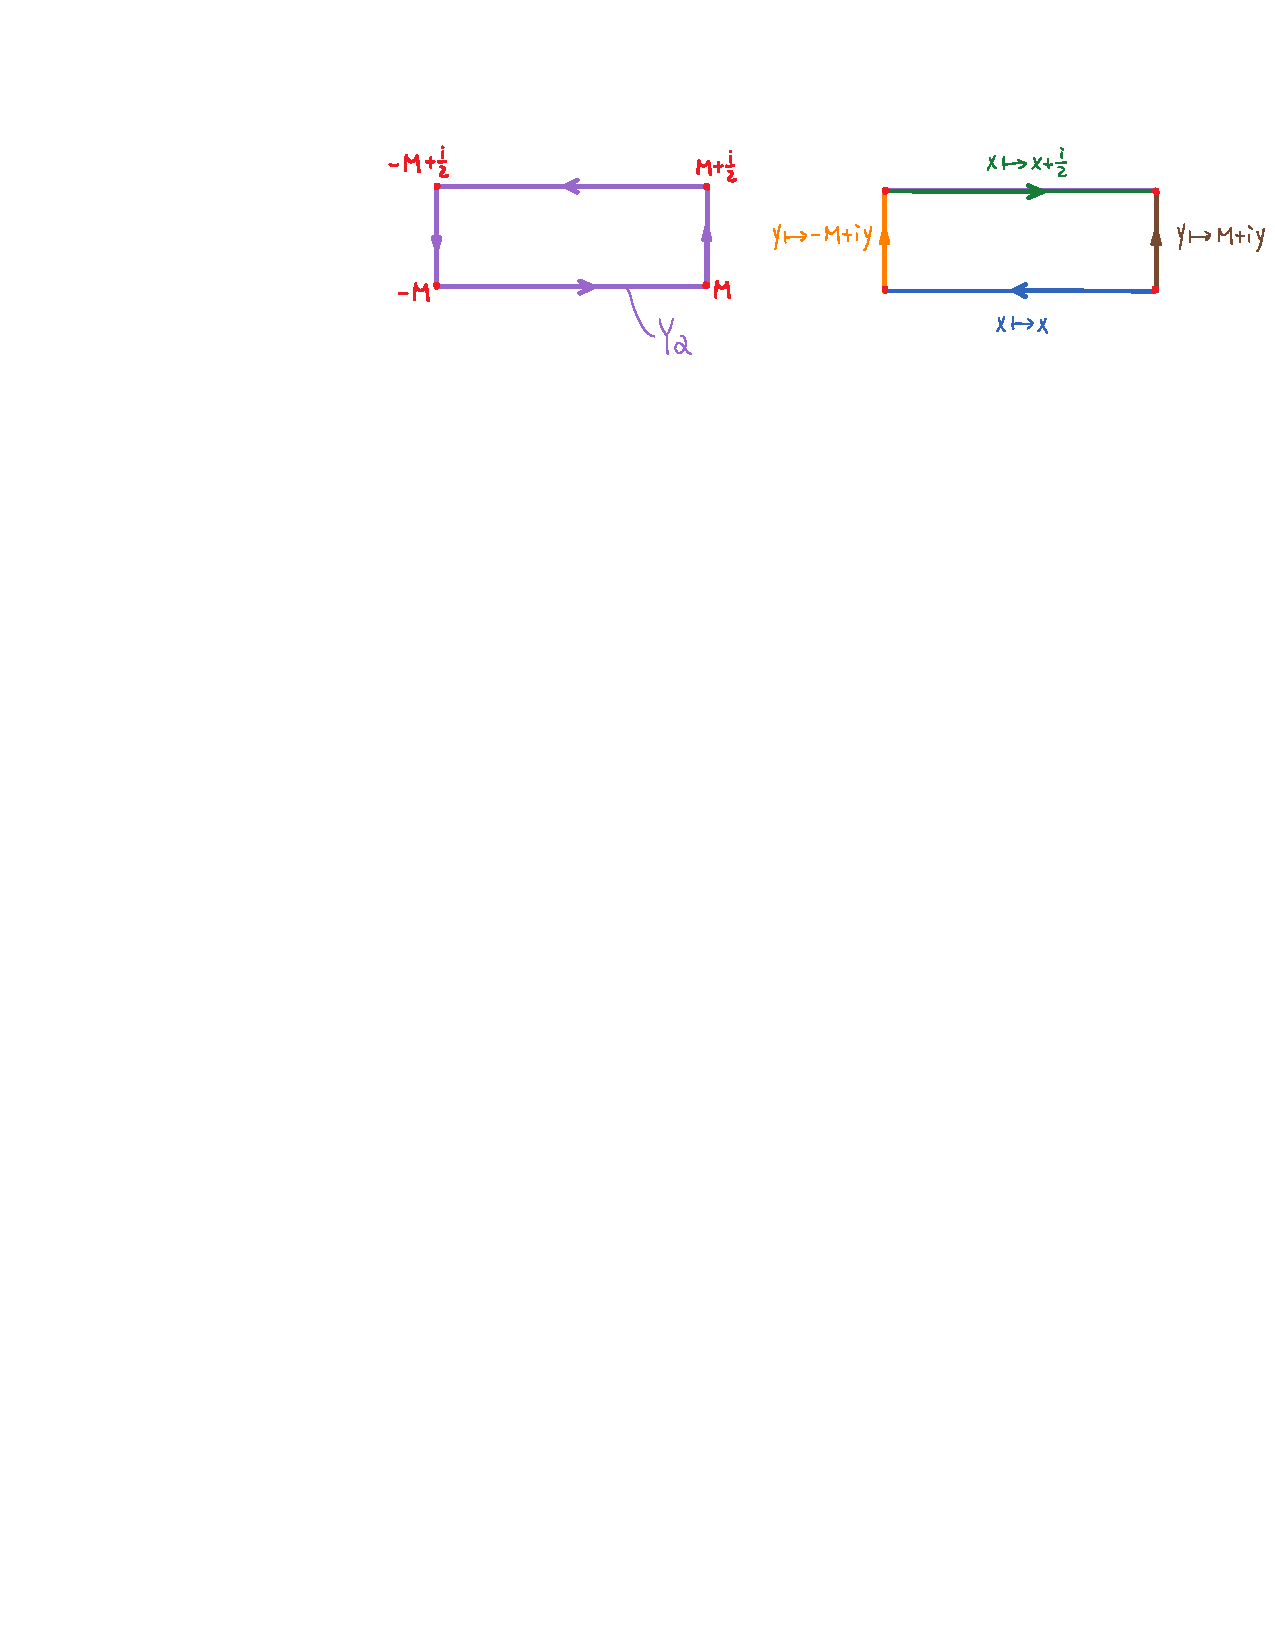
\includegraphics[scale=0.9]{paths.pdf}
\end{center}

By Cauchy Integral Theorem, we have $\int_{Y_\alpha} e^{-z^2} dz = 0$, but here we can also write:
\begin{align*}
\int_{Y_\alpha}e^{-z^2} dz 
=& +\int_{-M}^M e^{-x^2}\, dx - \int_{-M}^M e^{-\left(x+\frac{i}{2}\right)^2} \,dx \\
&+ \int_{0}^{1/2} e^{-(M+iy)^2} \, dy - \int_0^{1/2}e^{-(-M+iy)^2}\, dy\\
=& + \int_{-M}^M e^{-x^2}\, dx - \int_{-M}^M e^{-x^2 - ix + \frac{1}{4}} \, dx \\
&+ \int_0^{1/2} e^{-M^2 - i2My + y^2} \, dy - \int_0^{1/2} e^{-M^2 + i2My + y^2} \, dy
\end{align*}
Now suppose $M$ approaches infinity, the following term vanishes:
$$\int_0^{1/2} e^{-M^2 - i2My + y^2} \, dy - \int_0^{1/2} e^{-M^2 + i2My + y^2} \, dy$$
 
In which case we obtain the following:
\begin{align*}
\int_{-\infty}^{\infty} e^{-x^2} \, dx = e^{1/4} \int_{-\infty}^\infty e^{-x^2} (\cos(x) - i \sin(x)) \, dx
\end{align*}
where we have: 
$$\sqrt{\pi} = \int_{-\infty}^{\infty} e^{-x^2} \, dx$$
Hence we see that:
$$0 = -e^{1/4} \int_{-\infty}^{\infty} e^{-x^2} \sin(x) \, dx\qquad\qquad \sqrt{\pi} = e^{-1/4} \int_{-\infty}^\infty e^{-x^2} \cos(x) \, dx$$
Rearranging we can write the following:
\begin{align*}
\int_{-\infty}^{\infty} e^{-x^2} \cos(x) \, dx = e^{-1/4} \sqrt{\pi}
\end{align*}

\hfill\break
\hfill\break
\exercise\footnote{In Fourier analysis, one can build generation functions from $\cos(ax)$ and $\sin(ax)$. \\ ${}$\qquad That is, the decomposition of a function $f(x)$ relies on the followings:
$$\int_{-\infty}^\infty f(x) \cos(ax)\, dx \qquad\qquad\qquad\qquad \int_{-\infty}^\infty f(x) \sin(ax)\, dx$$} $$\int_{-\infty}^{\infty} e^{-x^2} \cos(ax)\,dx = e^{-a^2/4} \sqrt{\pi}$$


\hfill\break

\begin{defn}
The orientation of a $1$-manifold in $\R^n$ can be viewed as the direction of motion on the manifold, and one might argue the positive tangent vectors point in the direction of forward motion. While now we suppose a compact $1$-manifold in $\R^2$, and suppose $\R^2 \setminus M$ is disconnected and has two components, the default orientation of $M$ is set by the condition that if we travel along $M$, then the bounded component of $\R^2 \setminus M$ lies to the left.
\end{defn}

\begin{thm}[Cauchy Integral Theorem]
Let $C_1$ and $C_2$ be disjoint circles in $\Complex$ with $C_2$ lying inside $C_1$, let $A$ be an open set of points lying inside $C_1$ and outside of $C_2$, let $U$ be an open subset of $\Complex$ containing $A\cup C_1 \cup C_2$, and let $f$ be a holomorphic function on $U$, then we have the following holds: $$\int_{C_1} f \, dz = \int_{C_2} f\, dz$$ 
\end{thm}
\begin{proof}
This theorem is a consequence of Theorem 37.2 on Munkres. While alternatively, we can consider the following proof. First construct a regular $P$-gon inscribed in $C_2$ so that $P$ and all points lying between $P$ and $C_2$ are contained in $U$. Use the $n$ rays from the center of $C_2$ through vertices of $P$ to divide $A$ into $n$ pieces with each piece bounded by a piecewise $C^1$ curve $Y_j$ consisting of an arc of $C_1$, an arc of $C_2$ and two ray segments. Note that by
pushing the arc of $C_2$ out to the corresponding side of $P$ we obtain a compact convex set $K\subseteq U$ containing $Y_j$. Slightly pushing out the pieces of $\Bd(K_j)$ we obtain an open convex set $V_j \subseteq U$ containing $Y_j$. Then by Corollary 22.1.1, we know that $\int_{Y_j} f\, dz = 0$. Summing over $Y_j$ we obtain the desired result. 
\end{proof}

\begin{corT}
Let $U$ be an open subset of $\Complex$ with some $z_0 \in U$, let $f$ be a holomorphic function defined on $U\setminus \{z_0\}$, then for $K = \{z \in \Complex \mid ||z - z_0|| = r\} \subseteq U$, we have $\frac{1}{2\pi i}\int_K f\, dz$ being independent of $r$. 
\end{corT}

\begin{defn}
Let $U$ be an open subset of $\Complex$ with some $z_0 \in U$, let $f$ be a holomorphic function defined on $U\setminus \{z_0\}$, then for $K = \{z \in \Complex \mid ||z - z_0|| = r\} \subseteq U$. The residue of $f\, dz$ at $z_0$, denoted as $Res(f\,dz, z_0)$, is defined by the following: $$Res(f\,dz, z_0)\coloneqq \frac{1}{2\pi i}\int_K f\, dz$$
\end{defn}


\begin{thm}
Let $U$ be an open subset of $\Complex$, let $D$ be a closed disc in $U$ with $z_0 \in \Int(D)$, and let $f$ be a holomorphic function defined on $U \setminus \{ z_0\}$. We have the following holds:
$$\int_{\Bd(D)} f\, dz = 2\pi i \, Res(f\, dz, z_0)$$
\end{thm}
\begin{proof}
Theorem 22.3 follows immediately from the Fundamental Theorem of Laziness.
\end{proof}


Let $g$ be a holomorphic function defined on an open subset $U$ of $\Complex$ with $z_0 \in U$.\\ 
We have the following holds:
\begin{align*}
Res\left(\frac{g(z)}{z-z_0}\, dz, z_0\right) &= \frac{1}{2\pi i}\int_{||z-z_0||=r} \frac{g(z)}{z-z_0}\, dz \\
&=\frac{1}{2\pi i} \int_0^{2\pi} \frac{g(z_0+re^{it})}{re^{it}}ire^{it}\, dt \\
&=\frac{1}{2\pi}\int_0^{2\pi} g(z_0+re^{it})\, dt\\
&= \frac{1}{2\pi}\,\left(\lim_{r \to 0}\int_0^{2\pi} g(z_0+re^{it})\, dt\right)\\
&= \frac{1}{2\pi}\, \int_0^{2\pi} g(z_0)\, dt\\
&= g(z_0)
\end{align*}
Note that, since $g$ is continuous at $z_0$, $g(z_0+re^{it})$ converges uniformly to $g(z_0)$ as $r$ approaches $0$.\\


\newpage
\subsection*{ML-Estimate}


\begin{prop}[ML-estimate in $\R^n$]
Let $Y_\alpha \subseteq \R^n$ be a parametrized $1$-manifold parametrized by $\alpha:[a,b] \to Y_\alpha$. Let $\omega$ be a $1$-form defined on an open subset of $\R^n$ containing $Y_\alpha$. Let $\text{length}(Y_\alpha)$ denote the $1$-volume of the manifold $Y_\alpha$. Then we have the following holds:
\begin{align*}
\left|\left|\int_{Y_\alpha} \omega \right|\right| \leq \sup_{\vec{v}\in Y_\alpha}||\omega(\vec{v})|| \cdot \text{length}(Y_\alpha)
\end{align*}
\end{prop}
\begin{proof}
Here we can write the following:
\begin{align*}
\left|\left|\int_{Y_\alpha} \omega \right|\right|= \left|\left|\int_a^b (\omega\circ \alpha) \cdot \alpha' \right|\right|
&\leq \int_a^b ||(\omega\circ \alpha) \cdot \alpha'||\\
&\leq \int_a^b ||\omega\circ \alpha|| \cdot ||\alpha'||\\
&\leq \sup||\omega|| \cdot \int_a^b d\mathcal{V}\\
&= \sup||\omega|| \cdot \text{length}(Y_\alpha)
\end{align*}
The result follows.
\end{proof}


\begin{thm}[ML-estimate in $\Complex$]
Let $Y_\alpha \subseteq \Complex$ be a parametrized $1$-manifold parametrized by $\alpha:[a,b] \to Y_\alpha$. Let $f:A \to \Complex$ be a continuous function with $A$ being an open open subset of $\Complex$ containing $Y_\alpha$. Let $\text{length}(Y_\alpha)$ denote the $1$-volume of $Y_\alpha$. Then we have the following holds:
\begin{align*}
\left|\left|\int_{Y_\alpha} f\, dz \right|\right| \leq \sup_{z \in Y_\alpha} |f(z)| \cdot \text{length}(Y_\alpha)
\end{align*}
\end{thm}
\begin{proof}
Note that we have $dz = \bmat{1&i}$, we can write the following:
\begin{align*}
\int_{Y_\alpha} f\, dz = \int_a^b f(t) \bmat{1 & i} \bmat{\alpha'_1(t) \\ \alpha'_2(t)} \, dt = \int_a^b f(t)\cdot (\alpha'_1(t) + i \alpha'_2(t))\, dt
\end{align*}
Hence we have:
\begin{align*}
\left|\left|\int_{Y_\alpha} f\, dz\right|\right| \leq \int_a^b |f(t)|\cdot ||\alpha'(t)||\, dt \leq \sup_{Y_\alpha} |f| \cdot \text{length}(Y_\alpha)
\end{align*}
The result follows.
\end{proof}



\newpage
\section[Complex Differentiability]{\color{red}Complex Differentiability\color{black}}

Consider $dz = dx+idy$ and $d\bar{z} = dx-idy$, we have: 
$$dx = \frac{dz+d\bar{z}}{2}\qquad\qquad\qquad\qquad\qquad dy = \frac{dz - d\bar{z}}{2}$$ 
Let $\alpha,\beta$ be $\Complex$-valued functions. We first show that $\alpha\, dx + \beta\, dy $ has one-to-one correspondence with some function $\Complex$-valued function $g,h$ such that $\alpha\, dx + \beta\, dy = g\, dz + h\, d\bar{z}$. Here we can write:
\begin{align*}
\alpha\, dx + \beta\, dy = \frac{\alpha-i\beta}{2} \, dz + \frac{\alpha + i\beta}{2}\, d\bar{z} \tag{E}
\end{align*}

Here we let $g,h$ be defined such that equation (E) holds, then the result follows.\\

Consider $f \in C^1(U, \Complex)$ with $f= u+iv$, where $U$ is an open subset of $\Complex$, first note that we can write:
\begin{align*}
Df = \bmat{D_1f & D_2f} = \bmat{D_1u + iD_1v & D_2u+iD_2v}
\end{align*}
Here we use $\frac{\partial f}{\partial x}$ to denote $D_1f$, and $\frac{\partial f}{\partial y}$ to denote $D_2f$. Then we can write the following:
$$df = \frac{\partial f}{\partial x}\, dx +\frac{\partial f}{\partial y}\, dy = \frac{1}{2}\left( \frac{\partial f}{\partial x}-i \frac{\partial f}{\partial y}\right) dz + \frac{1}{2}\left( \frac{\partial f}{\partial x}+i \frac{\partial f}{\partial y}\right) d\bar{z}$$
Here we let:
$$\frac{\partial f}{\partial z}\coloneqq \frac{1}{2}\left( \frac{\partial f}{\partial x}-i \frac{\partial f}{\partial y}\right)\qquad\qquad\qquad\quad\frac{\partial f}{\partial \bar{z}}\coloneqq \frac{1}{2}\left( \frac{\partial f}{\partial x}+i \frac{\partial f}{\partial y}\right)$$ Note that we have:
\begin{align*}
\frac{\partial f}{\partial x} = \frac{\pd f}{\pd z}+ \frac{\pd f}{\pd \bar{z}}\qquad\qquad\qquad\qquad\quad
\frac{\pd f}{\pd y}= i \frac{\pd f}{\pd z} - i \frac{\pd f}{\pd \bar{z}}
\end{align*}


\hfill\break
\begin{defn}
Let $U$ be an open subset of $\Complex$, let $f:U \to \Complex$ be a function. $f$ is said to be differentiable in real sense at $t \in U$ provided that $u:U \to \R \ \ \ z\mapsto\Re(f(z))$ and $v:U \to \R \ \ \ z\mapsto\Im(f(z))$ are both differentiable at $t$. Here we consider $\Complex \cong \R^2$ when evaluating the differentiability of $u$ and $v$.  
\end{defn}
\hfill\break
Here we note that, for $U$ being an open subset of $\Complex$, if a function $f:U \to \Complex$ is of $C^1$ type, then $f$ is differentiable in the real sense, but in the following discussion we will investigate how we can define the differentiability of the function $f$ in complex sense, given the additional algebraic structures of $\Complex$.\\

Now let $f$ be a function of $C^1$ type defined on $U$, where $U$ is an open subset of $\Complex$. Here we consider affine approximation of $f$ at $z_0 \in U$, for $z = x+iy$ in a small neighborhood of $z_0$, we can write:
\begin{align*}
f(z) 
&\approx f(z_0) + \frac{\pd f}{\pd x}(z_0)(x-x_0) +\frac{\pd f}{\pd y}(z_0)(y-y_0)\\ 
&= f(z_0) + \frac{\pd f}{\pd z}(z_0)(z-z_0) + \frac{\pd f}{\pd \bar{z}}(z_0)(\overline{z-z_0})
\end{align*}

By the differentiability of $f$ in real sense, we have the following holds:
\begin{align*}
 \lim_{(z-z_0) \to 0}\frac{f(z) - f(z_0) - \frac{\pd f}{\pd z}(z_0)(z-z_0) - \frac{\pd f}{\pd \bar{z}}(z_0)(\overline{z-z_0}) }{z-z_0} = 0
\tag{P}\end{align*}

We shall evaluate the following limit and define it as the complex derivative of $f$:
\begin{align*}
\lim_{(z-z_0)\to 0}\frac{f(z) - f(z_0)}{z-z_0} \tag{L}
\end{align*}

Suppose that we have $\frac{\partial f}{\partial \bar{z}}(z_0) =0$, then by (P) we get the following: 
\begin{align*}
\lim_{(z-z_0)\to 0}\frac{f(z) - f(z_0)}{z-z_0} = \frac{\pd f}{\pd z}(z_0)
\end{align*}
For notation, we denote:
\begin{align*}
\text{(F)} = \frac{f(z)-f(z_0)}{z-z_0}
\end{align*}
Here, on the other hand, if $\frac{\pd f}{\pd \bar{z}}(z_0) \neq 0$, we can write:
\begin{align*}
\text{(F)}=\frac{\pd f}{\pd z}(z_0) + \frac{\pd f}{\pd \bar{z}}(z_0)\frac{\overline{z-z_0}}{z-z_0}+\frac{f(z) - f(z_0) - \frac{\pd f}{\pd z}(z_0)(z-z_0) - \frac{\pd f}{\pd \bar{z}}(z_0)(\overline{z-z_0}) }{z-z_0}  
\end{align*}
Here $\frac{\pd f}{\pd z}(z_0)$ does not depend on $z-z_0$, while $\frac{\pd f}{\pd \bar{z}}(z_0)\frac{\overline{z-z_0}}{z-z_0} $ depends on $z-z_0$.\\ Denote $z-z_0 = he^{i\Phi}$ with $h = ||z-z_0||$, we can rewrite (F) as the following:
\begin{align*}
\text{(F)}=\frac{\pd f}{\pd z}(z_0) + \frac{\pd f}{\pd \bar{z}}(z_0)he^{-i2\Phi} +\frac{f(z) - f(z_0) - \frac{\pd f}{\pd z}(z_0)(z-z_0) - \frac{\pd f}{\pd \bar{z}}(z_0)(\overline{z-z_0}) }{z-z_0} 
\end{align*}
we see that if $\frac{\pd f}{\pd \bar{z}}\neq 0$, the limit (L) depends on $\Phi$, hence the limit is not defined.\\

When the limit (L) exists and is finite, $f$ is said to be complex differentiable, and we define the complex derivative of $f$ at $z_0$ as $f'_{\Complex}(z_0)\coloneqq \frac{\pd f}{\pd z}(z_0)$. Notice that, $f$ is of $C^1$ type, so $\frac{\pd f}{\pd z}(z_0)$ guarantees to exist, but $f$ might not be complex differentiable because $\frac{\partial f}{\partial \bar{z}}(z_0)$ might not necessarily be zero, and hence limit (L) might not necessarily exists. \\

\begin{defn}
Let $f$ be a function of $C^1$ type defined on $U$, where $U$ is an open subset of $\Complex$. $f$ is said to be complex differentiable, denoted as $\Complex$-differentiable, at $z_0\in U$ provided that $\frac{\partial f}{\partial \bar{z}}(z_0)= 0$. If $f$ is $\Complex$-differentiable, $f'_{\Complex}(z_0) = \frac{\pd f}{\pd z}(z_0)$ is called the derivative of $f$ at $z_0$.\footnote{$f'_{\Complex}(z_0)$ might be denoted as $f'(z_0)$ thereafter.}
\end{defn}

\begin{thm}
Let $f$ be a function defined on $U$, where $U$ is an open subset of $\Complex$. \\
The followings are equivalent:
\begin{enumerate}[topsep=3pt,itemsep=-1ex,partopsep=1ex,parsep=1ex]
\item $f$ is holomorphic on $U$
\item $f$ is of $C^1$ type on $U$, and $\frac{\pd f}{\pd \bar{z}} = 0$ 
\item $f$ is $\Complex$-differentiable at each point in $U$, and $f'_{\Complex}$ is continuous. 
\end{enumerate}
\end{thm}


\begin{corT}
Let $U$ be an open subset of $\Complex$, let $D\subseteq U$ be a closed disc with $z_0 \in \Int(D)$, and let $g$ be a holomorphic function defined on $U$. Then we have the followings:
$$\int_{z \in \Bd(D)} \frac{g(z)}{z-z_0}\, dz = 2\pi i g(z_0) \quad\qquad\qquad g'_{\Complex}(z_0) = \frac{1}{2\pi i}\int_{z\in \Bd(D)} \frac{g(z)}{(z-z_0)^2}\, dz$$
\end{corT}
\begin{proof}
We will show $\frac{g(z_0+h)-g(z_0)}{h}$ approaches $ \frac{1}{2\pi i}\int_{z\in \Bd(D)} \frac{g(z)}{(z-z_0)^2}$ as $h $ approaches $0$:
\begin{align*}
\frac{g(z_0+h)-g(z_0)}{h}= \frac{1}{2\pi i h}\int_{z\in \Bd(D)} g(z) \left( \frac{1}{z-z_0-h} - \frac{1}{z-z_0}\right)\, dz 
\end{align*}
Hence with ML-estimate, we see that:
\begin{align*}
(*)&\coloneqq  \left|\left|\frac{g(z_0+h)-g(z_0)}{h} -\frac{1}{2\pi i}\int_{z\in \Bd(D)} \frac{g(z)}{(z-z_0)^2}\, dz\right|\right| \\
&\leq \frac{\text{length}(\Bd(D))}{2\pi}\cdot |h|\cdot \left(\sup_{z \in \Bd(D)}|g(z)|\right)\cdot \frac{1}{(d(z_0,\Bd(D)) - |h|) \cdot d(z_0,\Bd(D))^2} 
\end{align*}
as $h$ approaches $0$, the fraction (*) approaches $0$. The result follows.
\end{proof}




\begin{corT}
Let $U$ be an open subset of $\Complex$, let $D\subseteq U$ be a closed disc with $z_0 \in \Int(D)$, and let $g$ be a holomorphic function defined on $U$. Then we have: 
$$g''_{\Complex}(z_0) = \frac{1}{2\pi i}\int_{\Bd(D)} \frac{2g(z)\, dz}{(z-z_0)^3}$$ 
That is, $g''_{\Complex}(z_0)$ exists.
\end{corT}

\begin{corT}[Differentiated Cauchy Integral Formula]
Let $U$ be an open subset of $\Complex$, let $D\subseteq U$ be a closed disc with $z_0 \in \Int(D)$, and let $g$ be a holomorphic function defined on $U$. Then we have:
$$g^{(m)}_{\Complex}(z_0) = \frac{m!}{2\pi i}\int_{z\in \Bd(D)}\frac{g(z)\, dz}{(z-z_0)^{m+1}}$$
The function $g$ is infinitely $\Complex$-differentiable.
\end{corT}

\newpage
\section[Complex Series]{\color{red} Complex Series \color{black}}
\begin{thm}[Taylor's Theorem]
Let $z_0 \in \Complex$, let $f$ be a holomorphic function defined on an open subset $\Omega$ of $\Complex$ that contains $z_0$. For all $z \in \Complex$ that satisfies $|z-z_0|<\rho$ for some $d(z_0, \Bd(\Omega))>\rho >0$, we have the following holds:
$$f(z) = \sum_{k=0}^\infty \frac{f^{(k)}_{\Complex}(z_0)}{k!}(z-z_0)^k$$
Here we denote $f^{(0)} \coloneqq f$, $0!\coloneqq 1$, and $(z-z_0)^0 \coloneqq 1$ for $z= z_0$. 
\end{thm}

\note ALTIR \footnote{\ "Ain't like this in $\R$."\hfill --\,David Barrett\ \ 1/24/2022}
\begin{enumerate}[topsep=3pt,itemsep=-1ex,partopsep=1ex,parsep=1ex]
\item In $\R$, the Taylor series in Theorem 24.1 could converge to the real-valued function $f$, example includes the function $f$ characterized by the following: $$f(x) = \begin{cases}e^{1/x} & x>0 \\ 0 & x\leq 0 \end{cases}$$ Note here $f^{(k)}(0) = 0$ for all $k$.
\item In $\R$, the Taylor series in Theorem 24.1 might not converge to $f$ except at the point of interest $z_0$.
Examples of these are connected with Stirling's Formula.  
\end{enumerate}
\remark All complex differentiable functions defined on an open subset of $\Complex$ is analytic.


\begin{proof}[Proof of Theorem 24.1]
Pick $0<r<\that{r} <\rho$. We will first prove the following Lemma:
\begin{lem}
\setlength{\leftskip}{1cm}
For $\zeta,z \in \Complex$, the series $$\sum_{k=0}^\infty \left( \frac{z-z_0}{\zeta - z_0}\right)^k$$
converges uniformly to the limit:
$$\frac{1}{1-\frac{z-z_0}{\zeta - z_0}}$$ 
for $\zeta$ and $z$ satisfies $|\zeta - z_0| = \that{r}$ and $|z-z_0| \leq r$.
\end{lem}

\begin{proof}
\setlength{\leftskip}{1cm} Here we can write:
$$\left|\frac{1}{1-\frac{z-z_0}{\zeta - z_0}} - \sum_{k=0}^m \left( \frac{z-z_0}{\zeta - z_0}\right)^k \right|=\left| \frac{\left(\frac{z-z_0}{\zeta - z_0}\right)^{m+1}}{1- \frac{z-z_0}{\zeta - z_0}}\right| \leq \frac{\left( \frac{r}{\that{r}}\right)^{m+1}}{1-\frac{r}{\that{r}}} \coloneqq (*)$$
Note that $(*)$ tends to $0$ when $m$ tends to infinity. \\
The result of the Lemma follows.
\end{proof}

By Cauchy Integral Formula, we have the following holds:
$$|z-z_0|\leq r \qquad\Rightarrow \qquad f(z) = \frac{1}{2\pi i} \int_{|\zeta - z_0|= \that{r}} \frac{f(\zeta)d\zeta}{\zeta - z}$$
Here we have:
\begin{align*}
\frac{1}{2\pi i} \int_{|\zeta - z_0|= \that{r}} \frac{f(\zeta)d\zeta}{\zeta - z} &= \frac{1}{2\pi i}\int_{|\zeta - z_0|= \that{r}} \frac{1}{\zeta - z_0} \frac{1}{1-\frac{z-z_0}{\zeta - z_0}} f(\zeta) \, d\zeta \\
&= \frac{1}{2\pi i} \int_{|\zeta - z_0| =\that{r}}\frac{1}{\zeta -z_0} \sum_{k=0}^\infty\left(\frac{z-z_0}{\zeta - z_0}\right)^k f(\zeta)\,d\zeta\\
&=\sum_{k=0}^\infty \frac{(z-z_0)^k}{2\pi i} \int \frac{f(\zeta)\, d\zeta}{(\zeta - z_0)^{k+1}} \\
&= \sum_{k=0}^\infty (z-z_0)^k \frac{f^{(k)}_{\Complex} (z_0)}{k!}
\end{align*}
This completes the proof.
\end{proof}

\begin{thm}
Let $f$ be a holomorphic function defined on a open subset $\Omega$ of $\Complex$. We denote: 
$$E \coloneqq  \bigcap_{k=0}^\infty (f_{\Complex}^{(k)})^{-1}(0)$$ 
If we have $\Omega$ being connected, then we have either $E = \emptyset$ or $f(z)= 0$ for all $z\in \Omega$. 
\end{thm}
\begin{proof}
Here we can write:
$$E = \{ z_0 \in \Omega \mid f_{\Complex}^{(k)}(z_0)=0 \ \forall k\in \N\cup \{0\} \} = \bigcap_{k=0}^\infty (f_{\Complex}^{(k)})^{-1}(0)$$
Since $f$ is continuous, then the preimage of a close set is relatively closed. Hence $(f_{\Complex}^{(k)})^{-1}(0)$ is closed for all $k$, and hence $E$ is relatively closed. Note that $E$ is open because if some $z_0 \in \Omega$ satisfies $f^{(k)}_{\Complex}(z_0) = 0$ for all $k \in \N \cup \{0\}$, then by Taylor's Theorem, there is a open neighborhood $B$ of $z_0$ such that $f^{(k)}_{\Complex}(z) = 0$ for all $z \in U$. Here we see that $E$ is both open and relatively closed, hence we must have either $E = \emptyset$ or $E = \Omega$. The result follows.
\end{proof}

\begin{corT}
Let $\Omega$ be a connected open subset of $\Complex$ that contains $z_0$, let $f_1$ and $f_2$ be holomorphic functions on $\Omega$, with $f_1^{(k)}(z_0) = f_2^{(k)}(z_0)$ for all $k$. 	Then we have $f_1(z) = f_2(z)$ for all $z \in \Omega$. 
\end{corT}

\begin{corT}
Let $\text{Holo}(A)$ denote the set of holomorphic functions defined on a set $A$. Let $V$ be an open connected subset of $\Complex$, let $U$ be a nonempty open proper subset of $V$. The restriction map from $\text{Holo}(V)$ to $\text{Holo}(U)$ is injective.
\end{corT}

\exercise ALTIR. Let $V$ be an open connected subset of $\Complex$, let $U$ be a nonempty open proper subset of $V$. The restriction map from $\text{Holo}(V)$ to $\text{Holo}(U)$ is not surjective.\footnote{Sometimes in several complex variables analysis, this is surjective}

\begin{thm}
For $z_0 \in \Complex$, consider the following power series:
\begin{align*}
\sum_{k=0}^\infty a_k(z-z_0)^k \tag{S}
\end{align*}
If $\sum_{k=0}^\infty a_k(z-z_0)^k$ converges pointwise on $|z-z_0| <r$ for some $r >0$. Then the function defined by the sum (S) is holomorphic on the set $\{ z \in \Complex \mid \, |z-z_0|<r\}$. 
\end{thm}
\begin{proof}
The proof of this theorem is given on Section 27 Theorem 6 in Spivak.
\end{proof}


\begin{thm}
Let $z_0 \in \Complex$, let $\Omega$ be a connected open subset of $\Complex$ that contains $z_0$, let $f$ be a holomorphic function defined on $\Omega$ and being not all zero on $\Omega$. Then there exists $m \in \N\cup\{0\}$ such that, for $z \in \Omega$, $f(z) = (z-z_0)^m h(z)$ with some holomorphic function $h$ defined on $\Omega$ and $h(z_0) \neq 0$. 
\end{thm}
\begin{proof}
Let $u = d(z_0, \Bd(\Omega))$. On $B_u (z_0)$, by Theorem 24.1, we have the Taylor series expansion for $f$ around $z_0$, here we can write the following, for $z \in \Omega$ that satisfies $|z-z_0|<u$, with $m=\min\{ k \in \N \cup \{0\} \mid f^{(k)}_\Complex(z_0 ) \neq 0 \}$ such that $a_m \neq 0$:
\begin{align*}
f(z) &= \sum_{k=m}^\infty a_k (z-z_0)^k
= (z-z_0)^m \sum_{k=m}^\infty a_k (z-z_0)^{k-m}
= (z-z_0)^m \sum_{j=0}^\infty a_{j+m} (z-z_0)^{j}
\end{align*}
Here we can define $h$ on $\Omega$ by the following:
\begin{align*}
h:\Omega \to \Complex \ \ \ z\mapsto \begin{cases}
\sum_{j=0}^\infty a_{j+m} (z-z_0)^{j} & z \in B_u (z_0)\\
\frac{f(z)}{(z-z_0)^m} & z \in \Omega\setminus \{z_0\}
\end{cases}
\end{align*}
The result follows.\\
\end{proof}

\begin{defn}
In the settings of Theorem 24.4, $m$ is called the order of $f$ at $z_0$, denoted as $\text{ord}_{z_0}f \coloneqq m$.
\end{defn}


\begin{corT}
Let $z_0 \in \Complex$, let $\Omega$ be a connected open subset of $\Complex$ that contains $z_0$, let $f$ be a holomorphic function defined on $\Omega$ with $f(z) \neq 0$ for some $z \in \Omega$. Then there exists $r>0$ such that $f(z) \neq 0$ for all $z \in \Omega$ that satisfies $0<|z-z_0|<r$. 
\end{corT}
\begin{proof}
One can make use of Theorem 24.4. Pick $r$ such that the function $h$ defined in Theorem 24.4 is nonzero on $|z-z_0|<r$. The result follows immediately.
\end{proof}

\begin{corT}
Let $K$ be a compact set that is contained in some connected open subset of $\Complex$, let $f$ be a holomorphic function defined on $\Omega$ with $f(z) \neq 0$ for some $z\in \Omega$. Then we have: 
$$\#(K\cap f^{-1}(0)) < \infty$$ 
\end{corT}
\begin{proof}
For each $z_i \in K$, since $f(z)\neq 0$ for some $z \in \Omega$, then by Corollary 24.4.1, there is a ball $B_{\epsilon_{z_i}}(z_i)$ such that $\#(B_{\epsilon_{z_i}}(z_i) \cap f^{-1}(0)) \in \{0,1\}$. Here $K \subseteq \bigcup_{i=1}^M B_{\epsilon_{z_i}}(z_i)$ for some $M \in \N$, then we have $\#(K\cap f^{-1}(0)) \leq M$. The result follows. 
\end{proof}

\begin{corT}
Let $f_1$ and $f_2$ be holomorphic functions on an open connected subset $\Omega$ of $\Complex$ with $f_1 = f_2$ on some infinite subset of a compact subset of $\Omega$. Then $f_1 = f_2$ on $\Omega$. 
\end{corT}

\begin{corL}[Persistence of Relations]
Let $f_1$ and $f_2$ be holomorphic functions defined on an open connected subset $\Omega$ of $\Complex$ that satisfies $\Omega \cap \R \neq \emptyset$.
If with $f_1(z) = f_2(z)$ for all $z \in \Omega\cap \R$, then we have $f_1 = f_2$ on $\Omega$. 
\end{corL}

\begin{defn}
A sequence on functions $(f_j)$ defined on $\Omega\subseteq \Complex$ is said to converge almost uniformly to a function $f$ defined on $\Omega$ provided that the sequence $(f_j)$ converges uniformly to $f$ on each compact subset $K$ of $\Omega$.
\end{defn}


\begin{thm}[Weierstrass Convergence Theorem]
The limit of a almost uniformly convergent sequence of holomorphic functions is holomorphic. 
\end{thm}

\begin{proof}
Let $(f_j)$ be a sequence of functions defined on an open subset $\Omega$ of $\Complex$. Suppose $(f_j)$ converges almost uniformly to a function $f $ defined on $\Omega$.  It suffices to show that $f$ is a holomorphic function on $\Int(D)$ where $D$ is a closed disc of $\Omega$. Note that by definition $f_j \, dz$ is closed in $\Omega$, hence by Theorem M.5 from Math 396 Supplement materials, $f_j \, dz$ is exact on $\Int(D)$, which, by Math 395 HW14 Q1, implies $f\, dz$ is exact on $\Int(D)$. Then we can write:
\begin{align*}
 f \, dz = dg = \frac{\partial g}{\partial z}\, dz + \frac{\partial g}{\partial \bar{z}}d\bar{z}
\end{align*}
Here we see that $\frac{\partial g}{\partial \bar{z}} = 0$, so $g$ is holomorphic, and hence $g'_{\Complex} = \frac{\partial g}{\partial z} = f$. By Differentiated Cauchy Integral Formula, we know that $f$ is holomorphic on $\Int(D)$. This completes the proof, but also note that ALTIR.
\end{proof}

Given power series: 
$$\sum_{n=0}^\infty a_n z^n$$
with $a_n, z \in Complex$, let $R$ be defined by:
$$R \coloneqq \frac{1}{\limsup_{n\to \infty} \sqrt[n]{|a_n|}} $$ and if $\limsup_{n\to \infty} \sqrt[n]{|a_n|}=0$, let $R \coloneqq \infty$, if $\limsup_{n\to \infty} \sqrt[n]{|a_n|} = \infty$, let $R = 0$. One can show that the series converges almost uniformly when $|z|<R$, and diverges when $|z|>R$.  \\

\exercise Let $z_0 \in \Complex$, let $(f_j)$ be a sequence of functions defined on an open set that contains $D = \{z \in \Complex \mid |z-z_0| < \rho\}$. $(f_j)$ converges almost uniformly to some function $f$ on $D$ if and only if $(f_j)$ converges uniformly to $f$ on each $D_r = \{ z \in \Complex |z-z_0|\leq r\}$ for all $r<\rho$. \\


\example
$$1-x^2 + x^4 -x^6+\cdots = \frac{1}{1+x^2} \qquad\qquad\qquad\text{ for }-1<x<1$$


\chapter{Differentiable Manifolds \ \rom{2}}
\setcounter{section}{24}
\section[Tensors]{\color{red}Tensors\color{black}}
\begin{defn}
Let $V$ be a vector space, denote $V_i = V$. For $k \in \N$, $V^k \coloneqq V_1 \times V_2 \times \cdots \times V_k$. $V^k$ is the set of $k$-tuples $(\vec{v}_1,\vec{v}_2,\cdots, \vec{v}_k)$ for vectors $\vec{v}_1,\vec{v}_2,\cdots, \vec{v}_k \in V$. 
\end{defn}

\begin{defn}
Let $V$ be a vector space, a function $f:V^k\to \R$ is said to be linear in the $i$-th variable provided that the function characterized by the following is linear:
$$T:V \to \R \ \ \ \vec{v}\mapsto f(\vec{v}_1,\cdots, \vec{v}_{i-1}, \vec{v}, \vec{v}_{i+1},\cdots, \vec{v}_k)$$
\end{defn}

\begin{defn}
Let $V$ be a vector space. A function $f:V^k \to \R$ is said to be multilinear provided that $f$ is linear in the $i$-th variable for all $1 \leq i \leq k$.  If $f$ is multilinear, then $f$ is called a $k$-tensor on $V$.
\end{defn}

\example The function $f$ defined by the following is a $2$-tensor: 
$$f:\R^2 \to \R \ \ \ \lr{\bmat{x_1\\y_1},\ \bmat{x_2\\ y_2}}\mapsto x_1y_2+x_2y_1$$

\example The function $f$ defined by the following is not a $2$-tensor: 
$$f:\R^2 \to \R \ \ \ \lr{\bmat{x_1\\y_1},\ \bmat{x_2\\ y_2}}\mapsto x_1y_1+x_2y_2$$

\begin{defn}
A $k$-tensor $f$ defined on a vector space $V$ is symmetric provided that the following holds:
$$f(\vec{v}_1,\cdots, \vec{v}_{i+1}, \vec{v}_i,\cdots, \vec{v}_k) = f(\vec{v}_1,\cdots, \vec{v}_{i}, \vec{v}_{i+1},\cdots, \vec{v}_k) $$ 
\end{defn}

\begin{defn}
A $k$-tensor $f$ defined on a vector space $V$ is alternating provided that the following holds:
$$f(\vec{v}_1,\cdots, \vec{v}_{i+1}, \vec{v}_i,\cdots, \vec{v}_k) = -f(\vec{v}_1,\cdots, \vec{v}_{i}, \vec{v}_{i+1},\cdots, \vec{v}_k) $$ 
\end{defn}

\note Let $f$ be a tensor defined on a vector space $V$. Let $\vec{v}_i = \vec{v}_j$ for some $i \neq j$. \\
$f$ is alternating if and only if we have $f(\vec{v}_1,\cdots, \vec{v}_{i}, \cdots \vec{v}_{j},\cdots, \vec{v}_k) = 0$. In other words, for $f \in \A^k(V)$, if we have $\#\{ i_1,i_2,\cdots, i_k\} < k$, then $f(\vec{v}_{i_1},\vec{v}_{i_2}, \cdots, \vec{v}_{i_k}) = 0$. 

\begin{defn}
Let $V$ be a vector space. We define the followings:\\
$\Lt^k(V)$ is the set of all $k$-tensor defined on $V$.\\
$\Symm^k(V)$ is the set of all symmetric $k$-tensor defined on $V$.\\
$\Alt^k(V)$, or denoted as $\A^k(V)$, is the set of all alternating $k$-tensor defined on $V$.
\end{defn}

\note For a vector space $V$, $\Lt^k(V)$, $\Symm^k(V)$, and $\A^k(V)$ are all vector spaces.\\ 
\note For a vector space $V$, $\Lt^1(V) = \Symm^1(V) = A^1(V)$ gives the dual space $V^*$ of $V$.\\


Let $V$ be a finite dimensional vector space with basis $(\vec{a}_1,\vec{a}_2,\cdots, \vec{a}_n)$. \\
For $\vec{a}\in V$, one can write $\vec{a} = \sum_n c_j \vec{a}_j$, then for a $k$-tensor $f$, we can write the following:
\begin{align*}
f\lr{\sum_{j_1=1}^n c_{1,j_1} \vec{a}_{j_1}, \right.&\left.\sum_{j_2=1}^n c_{2,j_2} \vec{a}_{j_2}, \cdots, \sum_{j_k=1}^n c_{k,j_k} \vec{a}_{j_k}} \\
&= \sum_{j_1=1}^n \left(c_{1,j_1}\cdot f\lr{\vec{a}_{j_1} , \sum_{j_2=1}^n c_{2,j_2} \vec{a}_{j_2}, \cdots, \sum_{j_k=1}^n c_{k,j_k} \vec{a}_{j_k}}\right) \\
&= \sum_{1\leq j_1, j_2,\cdots, j_k \leq n} c_{1,j_1}\cdot c_{2,j_2}\cdots \cdot c_{k,j_k}\cdot f(\vec{a}_{j_1}, \vec{a}_{j_2}, \cdots, \vec{a}_{j_k})  
\end{align*}
so the value of $f$ is completely determined by $f(\vec{a}_{i_1},\vec{a}_{i_2},\cdots, \vec{a}_{i_k})$, where $(\vec{a}_{i_1},\vec{a}_{i_2},\cdots, \vec{a}_{i_k})$ is some combination of the basis vectors $\vec{a}_1,\vec{a}_2,\cdots,\vec{a}_n$.\\
\hfill\break


Just as a linear transformation from vector spaces $V$ to $W$ can be defined by specifying its values arbitrarily on basis elements for $V$, a $k$-tensor defined on $V$ can be defined by specifying its values arbitrarily on $k$-tuples of basis elements. This fact is a consequence of the next theorem:

\begin{thm}
Let $V$ be an $n$-dimensional vector space with basis $(\vec{a}_1,\vec{a}_2,\cdots, \vec{a}_n)$, let $I = (i_1,i_2,\cdots, i_k)$ be a $k$-tuple of integers from the set $\{1,2,\cdots, n\}$. There exists a unique $k$-tensor $\Phi_I$ on $V$ such that for every $k$-tuple $M = (m_1,m_2,\cdots,m_k)$ of integers from the set $\{1,2,\cdots, n\}$, we have the following holds:
\begin{align*}
\Phi_I\left(\vec{a}_{m_1},\vec{a}_{m_2},\cdots, \vec{a}_{m_k},\right) = \begin{cases} 
0 & I \neq M \\
1 & I = M
\end{cases}
\end{align*}
\end{thm}

\begin{proof}
One can define $\Phi_I$ by the following:
\begin{align*}
\Phi_I:V^k \to \R \ \ \ \lr{\sum_{j_1=1}^n c_{1,j_1} \vec{a}_{j_1}, \sum_{j_2=1}^n c_{2,j_2} \vec{a}_{j_2}, \cdots, \sum_{j_k=1}^n c_{k,j_k} \vec{a}_{j_k}}\mapsto c_{1,i_1}\cdot c_{2,i_2} \cdot \cdots \cdot c_{k,i_k}  \tag{I}
\end{align*}
Here one can show that $\Phi_I$ satisfies the conditions and is a $k$-tensor. The rest of the proof of this theorem follows from Theorem 26.3 from on Munkres. 
\end{proof}
\newpage

If one define $\Phi_I$ with equation (I) by using the basis $(\vec{a}_1,\vec{a}_2,\cdots, \vec{a}_n)$ of $V$, then we have the following proposition, with the exact same settings as in Theorem 25.1:
\begin{prop}
Let $V$ be an $n$-dimensional vector space with a basis $(\vec{a}_1,\vec{a}_2,\cdots, \vec{a}_n)$, let $I = (i_1,i_2,\cdots, i_k)$ be a $k$-tuple of integers from the set $\{1,2,\cdots, n\}$. For $f \in \Lt^k(V)$, we have: 
$$f = \sum_I f(\vec{a}_I) \Phi_I$$ 
where we write $\vec{a}_I \coloneqq \left(\vec{a}_{m_1},\vec{a}_{m_2},\cdots, \vec{a}_{m_k},\right)$.
\end{prop}

\begin{proof}
The proposition follows immediately if one expand the equation $f = \sum_I f(\vec{a}_I) \Phi_I$.
\end{proof}

Given an $n$-dimensional vector space $V$ and a basis $(\vec{a}_1,\vec{a}_2,\cdots, \vec{a}_n)$, let $\Phi_I$ be defined with equation (I), we conclude that the set defined by the following forms a basis for $\Lt^k(V)$, denoted as the following:
\begin{align*}
\mathbb{P} \coloneqq \left\{ \Phi_I \mid I = (i_1,i_2,\cdots, i_k) \text{ is a }k\text{-tuple of integers from the set } \{1,2,\cdots, n\} \right\}
\tag{P}
\end{align*}

\remark The definition of $\mathbb{P}$ depends on the choice of basis of $V$. 

\begin{defn}
Let $V$ be a vector space. The tensor product operator $\otimes$ is defined to be the following:
\begin{align*}
\otimes: \Lt^k(V)\times \Lt^l(V) \to \Lt^k(V) \ \ \ (f,g)\mapsto f\otimes g
\end{align*}
where, for $f\in \Lt^k(V)$ and $g \in \Lt^l(V)$, we write:
\begin{align*}
f\otimes g : V^{k+l} &\to \R\\
(\vec{v}_1,\vec{v}_2,\cdots, \vec{v}_k, \vec{v}_{k+1},\cdots, \vec{v}_{k+l})&\mapsto f(\vec{v}_1,\vec{v}_2,\cdots, \vec{v}_k)\cdot g(\vec{v}_{k+1},\vec{v}_{k+2}, \cdots, \vec{v}_{k+l} )
\end{align*}
\end{defn}

\note Let $V$ be a vector space. \\
For $f \in \Lt^k(V)$, $h \in \Lt^m(V)$, and $g \in \Lt^l(V)$, and $c \in \R$, we have:
\begin{enumerate}[topsep=3pt,itemsep=-1ex,partopsep=1ex,parsep=1ex]
\item $(f\otimes g) \otimes h = f\otimes (g\otimes h)$
\item $(c\cdot f) \otimes g = c\cdot (f\otimes g) = f\otimes (c\cdot g)$
\item $(f+g) \otimes h = f\otimes h + g\otimes h$
\item $f\otimes (g+h) = f\otimes g+ f\otimes h$\\
\end{enumerate}

Let $V$ be an $n$-dimensional vector space over the field $F$, with basis $\mathbb{A} = (\vec{a}_1,\vec{a}_2,\cdots, \vec{a}_n)$, let $\mathbb{D} = (\Phi_1,\Phi_2,\cdots,\Phi_n)$ be the dual basis of $V$ associated to the basis $\mathbb{A}$, we can write:
\begin{align*}
\Phi_i: V \to F \qquad \sum_{j=1}^n t_j\vec{a}_j \mapsto t_i
\end{align*}
Note that $\mathbb{D}$ forms a basis of $\A^1(V)$. Moreover, let $\mathbb{P}$ be the basis of $\Lt^k(V)$ as defined by equation (P), for $\Phi_I \in \mathbb{P}$, we can write the following, with $I = (i_1,i_2,\cdots, i_k)$: $$\Phi_I \coloneqq \Phi_{i_1}\otimes \Phi_{i_2}\otimes \cdots \otimes \Phi_{i_k}$$

\begin{defn}
Let $V$ and $W$ be vector spaces, let $T:V \to W$ be a linear transformation. We define the dual transformation $T^*$ by the following:
\begin{align*}
T^*:\Lt^k(W) \to \Lt^k(V) \ \ \ f\mapsto T^*f
\end{align*}
where, for $f \in \Lt^k(W)$, and $\vec{v}_1,\vec{v}_2,\cdots, \vec{v}_k \in V$, we have:
\begin{align*}
T^*f:V^k \to \R \ \ \ (\vec{v}_1,\vec{v}_2,\cdots, \vec{v}_k ) \mapsto f\left(T(\vec{v}_1),T(\vec{v}_2),\cdots, T(\vec{v}_k) \right) 
\end{align*}
\end{defn}

\note In the settings of Definition 25.1.1.0.2, it is immediate that $T^*f$ is multilinear because $T$ is linear and $f$ is multilinear. It is also true that $T^*$ itself is linear, as map of tensors. Let $X$ be a vector space, and let $S:W \to X$ be a linear transformation, then we have the followings hold:
\begin{enumerate}[topsep=3pt,itemsep=-1ex,partopsep=1ex,parsep=1ex]
\item $T^*(f\otimes g) = T^*f \otimes T^* g$ for all $f,g \in \Lt^k(W)$
\item $(S\circ T)^*f = T^*(S^*f)$ for all $f \in \Lt^k(W)$
\end{enumerate}

\newpage
\section[The Permutation Group]{\color{red}The Permutation Group \color{black}}
\begin{defn}
Let $k \geq 2$. A permutation of the set of integers $K= \{1 , 2,\cdots, k\}$ is a bijection function $\sigma$ from $K$ to $K$. We denote the set of all such permutations by $S_k$. 
\end{defn}

\note For $k\geq 2$, if $\sigma, \tau \in S_k$, then $\sigma\circ \tau ,  \sigma^{-1} \in S_k$. The set $S_k$ equipped with function composition operation forms a group called the symmetric group, or the permutation group, on the set $\{1, 2,\cdots, k\}$. There are $k!$ elements in such group. \\

\begin{defn}
For $k\geq 2$, let $K \coloneqq \{ 1,2,\cdots, k\}$, given $1 \leq i \leq k$, let $e_i$ be the element of $S_k$ defined by: 
$$e_i : K \to K \ \ \ j \mapsto \begin{cases} j & j\neq i \text{ and } j\neq i+1\\
i+1 & j=i \\
i & j=i+1
\end{cases}$$
The element $e_i$ is called an elementary permutation on $K$. 
\end{defn}

\note In the settings of Definition 26.0.0.0.2, we have $e_i \circ e_i$ being the identity permutation, so $e_i$ is its own inverse in the group $S_k$ equipped with function composition operation. \\

\begin{lem}[Lemma 27.1 on Munkres]
Let $\sigma \in S_k$, $\sigma$ is a composition of elementary permutations in $S_k$. 
\end{lem}

\begin{defn}
Let $\sigma \in S_k$. Consider the set of all pairs of integers $(i, j)$ from the set $K \coloneqq \{1,2,\cdots, k\}$, for which $i<j$ and $\sigma(i) > \sigma(j)$. Each such pair is called an inversion in $\sigma$. We define the sign of $\sigma$, denoted as $\sgn(\sigma)$, or $\sgn \sigma$ by the following:
\begin{align*}
\sgn: S_k \to \{0,1\} \ \ \ \sigma\mapsto \begin{cases}
1 & \text{ the number of inversion in }\sigma \text{ is even}\\
-1 & \text{ the number of inversion in }\sigma \text{ is odd}
\end{cases}
\end{align*}
We call $\sigma$ an odd or even permutation according to the sign of $\sigma$ equals to $-1$ or $+1$, respectively. 
\end{defn}

\begin{lem}[Lemma 27.2 on Munkres]
Let $\sigma \in S_k$. If $\sigma $ is a composition of $m$ elementary permutations, then $\sgn (\sigma) = (-1)^m$.
\end{lem}

\begin{lem}[Lemma 27.2 on Munkres]
Let $\sigma ,\tau \in S_k$, we have $\sgn(\sigma\circ \tau) = \sgn(\sigma) \cdot \sgn(\tau)$, and $\sgn(\sigma^{-1}) = \sgn(\sigma)$. 
\end{lem}

\begin{lem}[Lemma 27.2 on Munkres]
For $p,q \in \{1,2,\cdots, k\}$ with $p \neq q$, if $\tau$ is a permutation in $S_k$ that exchanges $p$ and $q$ and leaves all other integers fixed, then $\sgn(\tau) = -1$. 
\end{lem}


\newpage
\section[The Wedge Product]{\color{red}The Wedge Product\color{black}}

\begin{defn}
For a family $I \in \{1,2,\cdots, n\}^k$, $I=(i_1,i_2,\cdots, i_k)$ is said to be ascending provided that we have: \footnote{Here $\{1,2,\cdots, n\}^k$ is viewed as a set of families. Each family in this set has entries from $\{1,2,\cdots, n\}$.} $$1\leq i_1< i_2,<\cdots <i_k\leq n$$ 
\end{defn}
\hfill\break
\note For a family $J=(j_1,j_2,\cdots, j_k) \in \{1,2,\cdots, n\}^k$. If $\#(\{j_1,j_2,\cdots, j_k\}) = k$, then there exists a unique $\sigma$, and a unique ascending $I=(i_1,i_2,\cdots, i_k) \in \{1,2,\cdots, n\}^k$ such that we have:
$$J = I_\sigma  \coloneqq (i_{\sigma(1)}, i_{\sigma(2)},\cdots, i_{\sigma(k)}) $$
Let $V$ be a vector space with basis $(\vec{a}_1,\vec{a}_2, \cdots, \vec{a}_n)$, and let $\mathbb{P}$ denote the basis of $\Lt^k(V)$ as defined in section 25 equation (P) in this text. For $f \in \A^k(V)$, we can write:
\begin{align*}
f = \sum\limits_{\substack{I \in \{1,2\cdots,n\}^k \\ I \text{ has no duplicate}}} f(\vec{a}_I) \Phi_I &= \sum\limits_{\substack{I \in \{1,2\cdots,n\}^k \\ I \text{ is ascending}}} \sum_{\sigma \in S_k} f(\vec{a}_{I_\sigma}) \Phi_{I_\sigma}
\end{align*}
Note that $f(\vec{a}_{I_{\sigma}}) = \sgn(\sigma) f(\vec{a}_I)$ because $f$ is alternating, then we can write:
\begin{align*}
f =\sum\limits_{\substack{I \in \{1,2\cdots,n\}^k \\ I \text{ is ascending}}} \sum_{\sigma \in S_k} \sgn (\sigma) f(\vec{a}_{I}) \Phi_{I_\sigma} 
= \sum\limits_{\substack{I \in \{1,2\cdots,n\}^k \\ I \text{ is ascending}}} f(\vec{a}_{I}) \sum_{\sigma \in S_k} \sgn (\sigma)  \Phi_{I_\sigma} \tag{A}  
\end{align*}
For ascending $I$, we define the following: 
$$\Psi_{I}\coloneqq \sum_{\sigma \in S_k} \sgn(\sigma) \Phi_{I_{\sigma}}$$
From equation (A), we see that the set defined by the following forms a basis for $\A^k(V)$:
\begin{align*}
\mathbb{S} \coloneqq \left\{ \Psi_{I} \mid I \text{ is an ascending }k\text{-tuple in }\{1, 2, \cdots, n\}^k\right\}
\end{align*}
Note here the definition of $\mathbb{S}$ depends on the definition of $\mathbb{P}$, and the definition of $\mathbb{P}$ depends on the choice of the basis of $V$, so we know that the definition of each elements in the basis $\mathbb{S}$ of $\A^k(V)$ depends on the choice of basis of $V$.\\

In such setting, if we have $k>n$, then $A^k(V) = \{ \vec{0}\}$. If we have $1\leq k \leq n$, then the dimension of $\A^k(V)$ equals to the cardinality of ascending $k$-tuples in $\{1,2,\cdots, n\}^k$, which is equals to $C_n^k$. Moreover, we have $\A^n(V) = \spa(\{\Psi_{(1,2,\cdots, n)}\})$. We further notice that, for $f\in \A^k(V)$ and $g \in \A^l(V)$, $f\otimes g$ might not necessarily belongs to $\A^{k+l}(V)$.\\


\note Let $V$ be a finite dimensional vector space with basis $(\vec{a}_1,\vec{a}_2,\cdots, \vec{a}_n)$. Let $(\Phi_1,\Phi_2,\cdots, \Phi_n)$ be the dual basis of $V^* = \Lt^1(V) = \A^1(V)$. For $I = (i_1,i_2,\cdots, i_k) \in \{1,2,\cdots, n\}^k$, let $\Phi_I = \Phi_{i_1}\otimes \Phi_{i_2} \otimes \cdots \otimes \Phi_{i_k}$, the following set forms a basis for $\Lt^k(V)$: 
$$\{\Phi_I\mid I = (i_1,i_2,\cdots, i_k) \in \{1,2,\cdots, n\}^k\}$$ For ascending $I= (i_1,i_2,\cdots, i_k)$, set $\Psi_I  = \sum_{\sigma \in S_k}\text{sgn}(\sigma) \Phi_{I_{\sigma}}$, here $I_{\sigma} = (i_{\sigma(1)},\cdots, i_{\sigma(k)})$, and $\Psi_I \in \A^k(V)$. $\{\Psi_I \mid I= (i_1,i_2,\cdots, i_k) \text{ is ascending}\}$ forms a basis for $\A^k(V)$. 
\begin{thm}
Let $V$ be a vector space, there exists a function $W$ characterized by the following: 
$$W:\A^k(V) \times \A^l(V) \to \A^{k+l}(V) \ \ \ (f,g)\mapsto f \wedge g$$ 
such that $f\wedge g \in \A^{k+l}(V)$ for $f \in \A^k(V)$, $g \in \A^l(V)$, and satisfies all of the followings:
\begin{enumerate}[topsep=3pt,itemsep=-1ex,partopsep=1ex,parsep=1ex]
\item For $f \in \A^k(V)$, $g \in \A^l(V)$, and $h \in \A^m(V)$, we have $f\wedge(g\wedge h) = (f\wedge g) \wedge h$
\item For $f \in \A^k(V)$, $g \in \A^l(V)$, and scalar $c$, we have $(c\cdot f) \wedge g = c\cdot (f\wedge g) = f\wedge (c\cdot g)$
\item For $f,g \in \A^k(V)$ and $h \in \A^l(V)$, we have $h\wedge (f+g) = h\wedge f + h\wedge g$, and we have $(f+g)\wedge h = f\wedge h + g \wedge h$
\item For $f \in \A^k(V)$ and $g \in \A^l(V)$, we have $g\wedge f = (-1)^{kl} \cdot f\wedge g$
\item Given a finite basis of $V$, let $(\Phi_i \mid 1 \leq i \leq n)$ be the corresponding dual basis for $V^*$, and let $(\Psi_I\mid I \text{ is an ascending }k\text{-tuple}\text{ of integers from the set }\{1,2,\cdots, n\})$ be the corresponding family of elementary alternating tensors. For any  ascending $k$-tuple $I = (i_1,i_2,\cdots, i_k)$ of integers from the set $\{1,2,\cdots, n\}$, we can write $\Psi_I = \Phi_{i_1}\wedge \Phi_{i_2}\wedge \cdots \wedge \Phi_{i_k}$. 
\item Let $T:V\to W$ be a linear transformation with $W$ being a vector space, let $f$ and $g$ be alternating tensors on $W$, then we have $T^*(f\wedge g) = T^*f \wedge T^* g$. 
\end{enumerate}
\end{thm}

\begin{proof}
Let $[I]$ denote the set of ascending $k$-tuple with entry from $Z = \{1,2,\cdots,n \}$, and let $[J]$ denote the set of ascending $l$-tuple with entry from $Z$, let $f = \sum_{I \in [I]} \alpha_I \Psi_I$ and $g = \sum_{J\in [J]}\beta_J \Psi_J$. Then we can define:
\begin{align*}
f \wedge g \coloneqq \sum\limits_{\substack{I\in [I], \ J\in [J]\\ no \ duplicates}} \alpha_I \beta_I \Psi_I \wedge \Psi_J \coloneqq \sum\limits_{\substack{I\in [I], \ J\in [J]\\ no \ duplicates}} \alpha_I  \beta_J \, \text{sgn}(I,J) \Psi_{sort(I,J)}
\end{align*}
here no duplicate means $I\cap J = \emptyset$, $(I,J)$ denote the $(k+l)$-tuple with the first $k$ entries being $I$ and then the last $l$ entries being $K$, $sort$ denote the function that sorts entries in the concatenated $(k+l)$-tuple $(I,J)$, which is equivalent to apply a corresponding permutation $\sigma_{IJ}$ to the tuple $(I,J)$ that sorts $(I,J)$, and $\text{sgn}(I,J)$ denotes $\sgn(\sigma_{IJ})$.\\ 

Here (2), (3), and (5) are cleared from such definition. \\

For (4), we consider the special case $f = \Psi_I$ and $g = \Psi_J$. It takes $kl$ steps to go from $(J,I)$ to $(I,J)$, that is, we have $\text{sgn}(J,I) = (-1)^{kl}\text{sgn}(I,J)$, so we have $\Psi_J \wedge \Psi_I  = (-1)^{kl}\Psi_I \wedge \Psi_J$. For a more general case, one can decompose the tensor using $\Psi_I$ and $\Psi_J$. \\

For (1), consider the special case where $f = \Psi_I$, $g = \Psi_J$, and $h = \Psi_K$, with $I,J,K$ being disjoint. Here we can write the following:
$$\text{sgn}(I,J)\cdot \text{sgn}(sort(I,J),K) = \text{sgn}(I, sort(J,K))\cdot \text{sgn}(J,K)$$ 
so $(\Psi_I \wedge \Psi_J) \wedge \Psi_K = \Psi_I \wedge (\Psi_J \wedge \Psi_k)$. The general case is left of exercise. \\

For (6), we first define the following function: 
$$\hat{A}: \Lt^k(V) \to \Lt^k(V) \ \ \ \ f\mapsto \sum_{\sigma \in S_k}\text{sgn}(\sigma) f^{\sigma}$$
where $f^\sigma(\vec{v}_1,\cdots, \vec{v}_k) \coloneqq f(\vec{v}_{\sigma(1)}, \cdots, \vec{v}_{\sigma(k)})$. It follows from Munkres Theorem 28.1 that we have $\hat{A}(f) \in \A^k(V)$ for all $f\in \Lt^k(V)$. Note that the definition for $\hat{A}$ does not rely on a basis of $V$. For ascending tuple $I$, we have $\hat{A}\Phi_{I} = \Psi_I$. Moreover, for $f \in \A^k(V)$, we have $f = \sgn(\sigma)f^\sigma$, hence we can write the following:
$$\hat{A}(f) =\sum_{\sigma \in S_k}\sgn(\sigma)\sgn(\sigma)f = \sum_{\sigma \in S_k} f = k! f$$
To completes the proof for (6), here we will make use of the following proposition:

\begin{prop}\setlength{\leftskip}{1cm}
Let $f \in \A^k(V)$ and $g \in \A^l(V)$, we have the following holds:
$$f\wedge g = \frac{1}{k!l!}\hat{A}(f\otimes g)$$
\end{prop} 
\begin{proof}\setlength{\leftskip}{1cm}
Consider the special case where $f = \Psi_I$ and $g = \Psi_J$ where $I$ is and ascending $k$-tuple and $J$ is an ascending $l$-tuple. It suffices to check that the following holds:
\begin{align*}
(\Psi_I \wedge \Psi_J)(\vec{a}_S) = \frac{1}{k!l!}\hat{A}(\Psi_I \otimes \Psi_J)(\vec{a}_S) \tag{*}
\end{align*}
for $S$ ascending $(k+l)$-tuples, with $\vec{a}_S = (\vec{a}_{s_1},\vec{a}_{s_2}, \cdots, \vec{a}_{s_{k+l}})$. Here $(\vec{a}_1,\vec{a}_2,\cdots,\vec{a}_n)$ is the basis of $V$ associated to the basis $(\Psi_K \mid K \text{ is ascending})$ of $\A^{k+l}(V)$. Note here we have:
\begin{align*}
\text{LHS of equation (*)} = \begin{cases}0 & I \cup J \neq S \\ \text{sgn}(I,J)& I \cup J = S \end{cases}
\end{align*}
Here we write $S_{\sigma} = (S_{\sigma}', S_{\sigma}'')$, where $S_{\sigma}'$ denotes the first $k$ entries of $S_{\sigma}$ and $S_{\sigma}''$ denotes the last $l$ entries of $S_{\sigma}$, then we can write the following:
\begin{align*}
\qquad\qquad\text{RHS of equation (*)} &= \frac{1}{k!l!}\sum_{\sigma \in S_{k+l}}\text{sgn}(\sigma) (\Psi_I \otimes \Psi_J ) (\vec{a}_{S_{\sigma}}) \tag{**}
\end{align*}
where we have, with some $\sigma' \in S_k$ and $\sigma'' \in S_l$:
\begin{align*}
\qquad\text{sgn}(\sigma) (\Psi_I \otimes \Psi_J ) (\vec{a}_{S_{\sigma}}) = \begin{cases} 0 & I\neq S_\sigma' \text{ or } J \neq S_\sigma'' \\ \text{sgn}(\sigma)\cdot \text{sgn}(\sigma')\cdot \text{sgn}(\sigma'')=\text{sgn}(I,J) & S_{\sigma} = (I_{\sigma'}, J_{\sigma''})\end{cases}
\end{align*}
Computing equation (**), the result follows.
\end{proof}
From Proposition 27.1.1, we also get the following property of the wedge product:
\begin{corT}\setlength{\leftskip}{1cm}
\setlength{\leftskip}{1cm} In the setting of Theorem 27.1, for $f \in \A^{k}(V)$ and $g \in \A^l(V)$, the value of $f \wedge g$ does not depend on the choice of basis of $V$.
\end{corT}
With Proposition 27.1.1, we get the following result:
\begin{align*}
T^*(f \wedge g) &= \frac{1}{k!l!} T^*\left(\sum_{\sigma \in S_{k+l}} \text{sgn}(\sigma) (f\otimes g)^\sigma\right)\\
&= \frac{1}{k!l!}\sum_{\sigma \in S_{k+l}} \text{sgn}(\sigma)T^*(f\otimes g)^\sigma\\
&= \frac{1}{k!l!}\sum_{\sigma \in S_{k+l}} \text{sgn}(\sigma)(T^*f \otimes T^* g)^\sigma\\
&= T^*f \wedge T^*g
\end{align*}
The results of Theorem 27.1 follows. 
\end{proof}

\hfill\break
\hfill\break
\hfill\break
\example\\
In the settings of Theorem 27.1 with $n=3$, let $\alpha, \beta, \gamma , \that{\alpha},\that{\beta},\that{\gamma}, \hat{\alpha},\hat{\beta},\hat{\gamma},A,B,C \in \R$.
\begin{align*}
(\alpha \Psi_1 + \beta \Psi_2 + \gamma \Psi_3) \wedge ( \that{\alpha} \Psi_1 + \that{\beta} \Psi_2 + \that{\gamma} \Psi_3) \wedge(\hat{\alpha}\Psi_1 + &\hat{\beta}\Psi_2 + \hat{\gamma}\Psi_3)  \\
&= \det\lr{\bmat{\alpha & \beta & \gamma \\ \that{\alpha}& \that{\beta}& \that{\gamma} \\ \hat{\alpha}& \hat{\beta}&\hat{\gamma}}} \Psi_{(1,2,3)}
\end{align*}
The wedge product of $n$ $1$-tensor gives determinant of the coefficients.
\begin{align*}
(\alpha \Psi_1 +\beta \Psi_2 + \gamma \Psi_3)\wedge (A\Psi_{(2,3)}-B\Psi_{(1,3)}+C\Psi_{(1,2)}) = (\alpha A + \beta B + \gamma C)\Psi_{(1,2,3)}
\end{align*}
The wedge product of an $1$-tensor with an (n-1)-tensor gives, sort of, with some sign issues, the dot product of the coefficients.
\begin{align*}
(\alpha \Psi_1 + \beta \Psi_2 +\gamma \Psi_3) \wedge (\that{\alpha} &\Psi_1 + \that{\beta} \Psi_2 + \that{\gamma} \Psi_3) \\
&= (\alpha \that{\beta} - \beta \that{\alpha})\Psi_{(1,2)} + (\beta \that{\gamma} - \gamma \that{\beta}) \Psi_{(2,3)} + (-\alpha \that{\gamma} + \gamma \that{\alpha}) \Psi_{(3,1)}
\end{align*}
The wedge product of $1$-tensor with $1$-tensor gives cross product of the coefficients. 

\newpage
\section[Differential Forms and Pullbacks]{\color{red}Differential Forms and Pullbacks\color{black}}
Let $\{\vec{e}_1,\vec{e}_2,\cdots,\vec{e}_n\}$ be the standard basis for $\R^n$. By our discussion in previous sections, we have $\Lt^1(\R^n) = \A^1(\R^n) = (\R^n)_{row}$, and the basis for $\Lt^1(\R^n)$ is given by: 
$$\{\vec{e}^T_j \mid 1 \leq j \leq n\}$$ 
Here we will, for most of the discussion, restrict our view to the standard basis of $\R^n$. 

\begin{defn}
Let $[I]$ denote the set of ascending $k$-tuples of integers from $\{1,2,\cdots, n\}$. \\
A $k$-form defined on an open subset $U$ of $\R^n$ is a continuous function defined by: 
$$\omega:U \to \A^k(\R^n) \ \ \ \vec{x}\mapsto \sum_{I \in [I]} b_I(\vec{x}) \Psi_I$$
where $b_I$ are continuous functions from $U$ to $\R$. \\The degree of a $k$-form is $k$, denoted as $\text{deg}(\omega) = k$. 
\end{defn}

Let $\omega$ be defined as in Definition 28.0.0.0.1, with standard basis of $\R^n$, here we have:
\begin{align*}
 \omega(\vec{x}) = \sum_{[I]} b_I(\vec{x}) \Psi_I 
 &= \sum_{[I]} b_I(\vec{x}) \Psi_{i_1}\wedge \Psi_{i_2}\wedge \cdots \wedge \Psi_{i_k}= \sum_{[I]} b_I(\vec{x})\, dx_{i_1}\wedge dx_{i_2}\wedge \cdots \wedge dx_{i_k} \tag{W}
\end{align*}

\begin{defn}
Let $U$ be an open subset of $\R^n$, let $k$-form $\omega$ be defined by:
$$\omega :U \to \A^k(\R^n) \ \ \ x\mapsto \sum_{I \in [I]} b_I(\vec{x}) \Psi_I $$ 
where $b_I$ are continuous functions from $U$ to $\R$. \\
$\omega$ is said to be of $C^r$ type provided that each $b_I$ is of $C^r$ type. 
\end{defn}

Let $U$ be an open subset of $\R^n$:\\
\remark A scalar function defined on $U$ can be viewed as a $0$-form defined on $U$. \\
\note The sum of two $k$-forms defined on $U$ is a $k$-form defined on $U$\\
\note A scalar function multiplied by a $k$-form defined on $U$ is a $k$-form defined on $U$.\\
\note A $k$-form wedge with a $l$-form, both defined on $U$, is a $(k+l)$-form defined on $U$,\\

\begin{defn}
Let $U$ be a subset of $\R^n$ and let $V$ be a subset of $\R^l$, let $\Phi:U \to V$ be a $C^1$ function, let $\omega$ be a $k$-form defined on $V$, then $\Phi^*\omega$ is a $k$-form defined on $U$ given by:
\begin{align*}
\Phi^*\omega: U \to \A^k(U) \ \ \ \vec{x}\mapsto (D\Phi(\vec{x}))^*\omega(\Phi(\vec{x}))
\end{align*}
where we have:
\begin{align*}
(D\Phi(\vec{x}))^*\omega(\Phi(\vec{x})): U^k &\to \R \\ 
(\vec{u}_1,\vec{u}_2,\cdots, \vec{u}_k) &\mapsto \omega(\Phi(\vec{x}))(D\Phi(\vec{x})(\vec{u}_1), D\Phi(\vec{x})(\vec{u}_2), \cdots , D\Phi(\vec{x})(\vec{u}_k))
\end{align*}
\end{defn}

\newpage
Now we need an exterior derivative operator $d$ that takes $k$-forms of $C^r$ type defined on $U$ to $(k+1)$-forms of $C^{r-1}$ type defined on $U$. Intuitively, we expect the operator $d$ to satisfy all of the following conditions:
\begin{enumerate}[topsep=3pt,itemsep=-1ex,partopsep=1ex,parsep=1ex]
\item $d$ is linear
\item $(d \circ d)$ should be a zero function. \\This is because the boundary of the boundary of a manifold get us an empty set
\item $d$ should satisfy some sort of product rule 
\end{enumerate} These expectation suggests a definition that we can write:

\begin{defn}
Let $\omega$ be the $k$-form defined by equation (W) and of $C^1$ type, $\omega$ is defined on an open subset $U$ of $\R^n$. $d(\omega)$ is defined to be the following: \footnote{$d(\omega)$ will be denoted as $d\omega$ thereafter.}
\begin{align*}
d\left( \omega \right):U \to \A^{k+1}(\R^n) \qquad \vec{x}\mapsto \sum_{[I]} db_I(\vec{x})\wedge dx_{i_1}\wedge dx_{i_2}\wedge \cdots \wedge dx_{i_k} 
\end{align*}
\end{defn}

\example
Let $\alpha:\R^2 \to \R$, $\beta:\R^2 \to \R$ be continuous functions.\\ 
Here $\omega = \alpha dx_1 + \beta \, dx_2$ is an $1$-form, and we can write the following:
\begin{align*}
d\left(\alpha\, dx_1+ \beta \, dx_2\right) &= \left(\frac{\partial \alpha}{\partial x_1}dx_1 + \frac{\partial \alpha}{\partial x_2}dx_2 \right)\wedge dx_1 + \left(\frac{\partial \beta}{\partial x_1}\, dx_1 + \frac{\partial \beta}{\partial x_2}\, dx_2 \right)\wedge dx_2 \\
&= \left( \frac{\partial \beta}{\partial x_1} - \frac{\partial \alpha}{\partial x_2}\right) dx_1\wedge dx_2
\end{align*}
\example Let $U$ be an open subset of $\R^n$, and let $\omega:U \to \R^n_{row} \ \ \ x\mapsto \sum_{j=1}^n b_j(\vec{x}) dx_j$ be a $1$-form of $C^1$ type, then by definition we can write the following:
\begin{align*}
d\lr{\sum_j b_j(\vec{x}) dx_j} = \sum_j \sum_k \frac{\pd b_j}{\pd x_k}dx_k \wedge dx_j = \sum_{j<k}\lr{\frac{\pd b_j}{\pd x_j} - \frac{\pd b_j}{\pd x_k}} dx_j \wedge dx_k
\end{align*}

\begin{defn}
A $k$-form $\omega$ is sad to be closed provided that we have $d\omega = 0$.
\end{defn}

\begin{lem}
For $k$-forms $\omega_1$ and $\omega_2$, we have $d(\omega_1 + \omega_2) = d\omega_1 + d\omega_2$.
\end{lem}
\begin{proof}
This lemma should follow from the definition.
\end{proof}

\begin{lem}
$d(\omega_1 \wedge \omega_2) = d\omega_1 \wedge \omega_2 +(-1)^{deg(\omega_1)}\, \omega_1\wedge d\omega_2$
\end{lem}
\begin{proof}
First note that for $0$-forms $f$ and $g$, we have $d(fg) = f\, dg+ df\, g$ for functions $f$ and $g$. Consider the key special case where $\omega_1 = \alpha\, dx_I$ and $\omega_2 = \beta\, dx_J$, where $\alpha$ and $\beta$ are $0$-forms. Here we can write the following:
\begin{align*}
d(\alpha\, dx_I \wedge \beta\, dx_J) &= d(\alpha\beta \, dx_I \wedge dx_J)  \\
&=  \beta \, d\alpha \wedge dx_I \wedge dx_J + \alpha\, d\beta \wedge dx_I \wedge dx_J \\
&= d(\alpha\, dx_I) \wedge (\beta\, dx_J) + (-1)^{deg(\alpha \, dx_I)} ( \alpha \, dx_I)\wedge d(\beta\, dx_J) 
\end{align*}
\end{proof} 

\begin{lem}
For a $k$-form $\omega$ of $C^2$ type, we have $d(d\omega) = 0$.
\end{lem}
\begin{proof}
If the degree of $\omega$ is zero, $d\omega$ is exact, and exact $1$-forms are closed, and hence the result follows. If the degree of $\omega$ is non-zero, we can write the following, with $\alpha_I$ being $0$-forms:
\begin{align*}
d\left( d\left(\sum_{[I]} \alpha_I dx_I \right) \right) = d\left(\sum_{[I]} d\alpha \wedge dx_I\right) = \sum_{[I]} d(d \alpha) \wedge dx_I - \sum_{[I]} d\alpha_I \wedge d(d x_I)
\end{align*}
Note here $d\alpha$ is an exact $1$-form, and $dx_j$ is exactly one form for all $j$, then we see that:
\begin{align*}
d\left( d\left(\sum_{[I]} \alpha_I dx_I \right) \right) =\sum_{[I]} d(d \alpha) \wedge dx_I - \sum_{[I]} d\alpha_I \wedge d(d x_I) = 0
\end{align*}
The result follows.
\end{proof}
\hfill\break


\begin{lem}
Let $U$ be a subset of $\R^l$ and let $V$ be a subset of $\R^n$, let $\Phi:U \to V$ be a $C^1$ function, let $\omega$ be a $k$-form defined on $V$ given by equation (W), we have $d(\Phi^* \omega) = \Phi^* d\omega$.
\end{lem}
\begin{proof}
A detailed proof of this Lemma is given on Theorem 32.3 in Munkres. If the degree of $\omega$ is zero, then we can rewrite $d(\Phi^* \omega)$  through Chain Rule and the result will follow. If the degree of $\omega$ is non zero, then we can write the following, summing over $[I]$:
\begin{align*}
d(\Phi^* \omega) &= \sum d\Phi^*(b_I dx_{i_1}\wedge dx_{i_2}\wedge \cdots \wedge dx_{i_k})\\
&= \sum d\left(\Phi^*b_I \cdot \Phi^*(dx_{i_1})\wedge \Phi^*(dx_{i_2})\wedge \cdots \wedge \Phi^*(dx_{i_k}) \right)\\
&= \sum d(\Phi^*b_I \cdot d(\Phi^*x_{i_1}) \wedge d(\Phi^*x_{i_2})\wedge \cdots \wedge d(\Phi^*x_{i_k}) )\\
&= \sum d(\Phi^*b_I) \wedge d(\Phi^*x_{i_1}) \wedge d(\Phi^*x_{i_2}) \wedge \cdots \wedge d(\Phi^*x_{i_k}) +0 \\
&= \sum \Phi^*db_I \wedge \Phi^* dx_{i_1} \wedge \Phi^* dx_{i_2} \wedge \cdots \wedge \Phi^* dx_{i_k}\\
&= \Phi^* d\omega
\end{align*}
\end{proof}

\newpage
\section[Integration of Differential Forms]{\color{red} Integration of Differential Forms \color{black}}
\begin{defn}
Let $U$ be a subset of $\R^k$ that is open in either $\R^k$ or $\mathbb{H}^k$, and let $\omega$ be a $k$-form defined on an open subset $U$ of $\R^k$ given by the following:
\begin{align*}
\omega:U \to \A^k(\R^k) \ \ \ \vec{x}\mapsto  f(\vec{x}) \,dx_1 \wedge dx_2 \wedge \cdots \wedge dx_k \tag{WF}
\end{align*}
where $f$ is a zero form defined on $U$. We define the following integral:
\begin{align*}
\int_U \omega \coloneqq \int_U f
\end{align*}
whenever $\int_U f$ exists.
\end{defn}
\note In the settings of Definition 29.0.0.0.1, the integral $\int_U \omega$ guarantees to exist if the support of the function $f$ is compact.\\

Let $U,V$ be subsets of $\R^k$ that are open in either $\R^k$ or in $\mathbb{H}^k$, such that there is a function $\Phi$ which defines a diffeomorphism from $U$ to $V$, with $\Phi_1, \Phi_2,\cdots, \Phi_k$ being component functions of $\Phi$, let $\omega$ be a $k$-form defined by equation (WF). Here we can write the following:
\begin{align*}
\int_U \Phi^*\omega &= \int_U \Phi^*f \cdot \Phi^*(dx_1)\wedge \Phi^*(dx_2)\wedge \Phi^*(dx_k)\\
&= \int_U (\Phi^* f) \cdot d\Phi_1 \wedge d\Phi_2 \wedge \cdots\wedge d\Phi_k \\
&= \int_U f\circ \Phi \cdot h(D\Phi) \cdot dx_1\wedge dx_2 \wedge \cdots \wedge dx_k
\end{align*}
Note here $h(D\Phi)$ is an alternating multilinear function of rows of $D\Phi$ with $h(I) = 1$ where $I$ is the identity matrix. One can show that we have $h(D\Phi) = \det(D\Phi)$, details can be found on Theorem 32.2 on Munkres, and then we can write the following:
\begin{align*}
\int_U \Phi^*\omega &= \int_U f\circ \Phi \cdot h(D\Phi) \cdot dx_1\wedge dx_2 \wedge \cdots \wedge dx_k\\
&= \int_U f\circ \Phi \cdot \det(D\Phi) \cdot dx_1\wedge dx_2 \wedge \cdots \wedge dx_k
\end{align*}
If $U$ is connected, or equivalently, if $V$ is connected, by the Change of Variable Theorem, we have:
$$\begin{cases}\int_U \Phi^*\omega =  \int_V f = \int_V \omega &  \det(D\Phi(\vec{x}))>0\ \ \ \forall/ \vec{x}\in U \\ \int_U \Phi^*\omega = - \int_V f = -\int_V \omega & \det(D\Phi(\vec{x}))<0\ \ \ \forall \vec{x}\in U \end{cases}$$ 
Note here $\det(D\Phi(\vec{x}))$ is nonzero for all $\vec{x}\in U$ because $\Phi$ is a diffeomorphism, and  $\det(D\Phi(\vec{x}))$ does not change sign for all $\vec{x}\in U$ if $U$ is connected. \\


\begin{defn}
Let $U$ be an open subset of $\R^k$, let $Y$ be a parametrized $k$-manifold in $\R^n$ parametrized by $\alpha:U \to Y$, let $\omega$ be a $k$-form defined on some open subset of $\R^n$ containing $Y$, we define the following integral:
\begin{align*}
\int_{Y_\alpha} \omega \coloneqq \int_U \alpha^*\omega
\end{align*} 
\end{defn}
\newpage

Consider a $k$-manifold $Y \in \R^n$ parametrized by $\alpha:U \to Y$, and can be reparametrized by $\that{\alpha}:V \to Y$, with $U,V$ being open subsets of $\R^k$. Let $\Phi$ denote a diffeomorphism between $U$ and $V$. 
\begin{center}
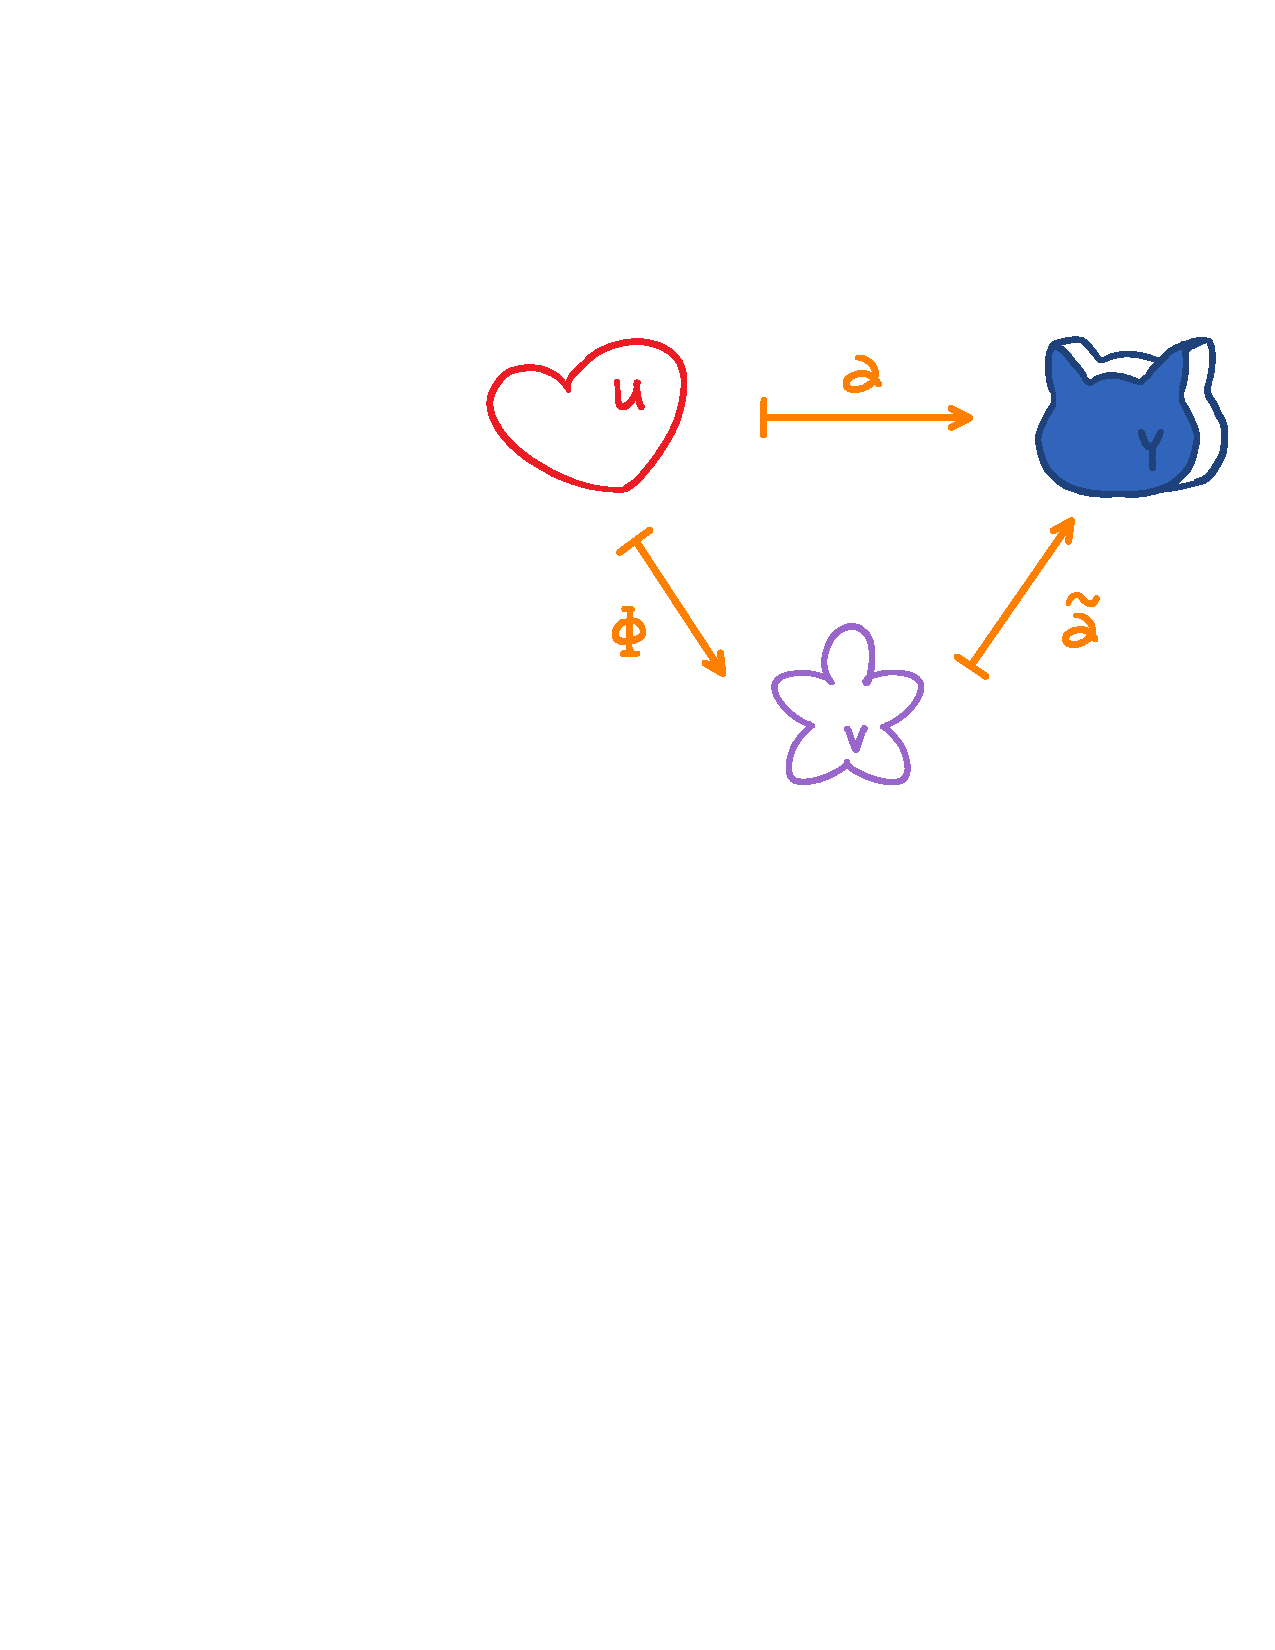
\includegraphics[scale=0.5]{Intkform.pdf}
\end{center}

Form argument in the discussion above, here we can write:
\begin{align*}
\int_{Y_\alpha} \omega = \int_V \that{\alpha}^*\omega &= \pm\int_U \Phi^*\that{\alpha}^*\omega = \pm \int_U \alpha^*\omega = \pm \int_{Y_\alpha} \omega
\end{align*}
The sign of $\pm \int_{Y_\alpha} \omega$ depends on the whether $\Phi$ is orientation preserving or orientation reversing, which we will discuss in the following section.\\



Now consider a $k$-manifold $Y \in \R^n$ parametrized by $\alpha:U \to Y$, with $U$ being open subsets of $\R^k$, let $\Phi$ denote a diffeomorphism between $Y$ and $\that{Y} \subseteq \R^n$, that is, $\that{Y}$ can be parametrized by $\Phi \circ \alpha$. 
\begin{center}
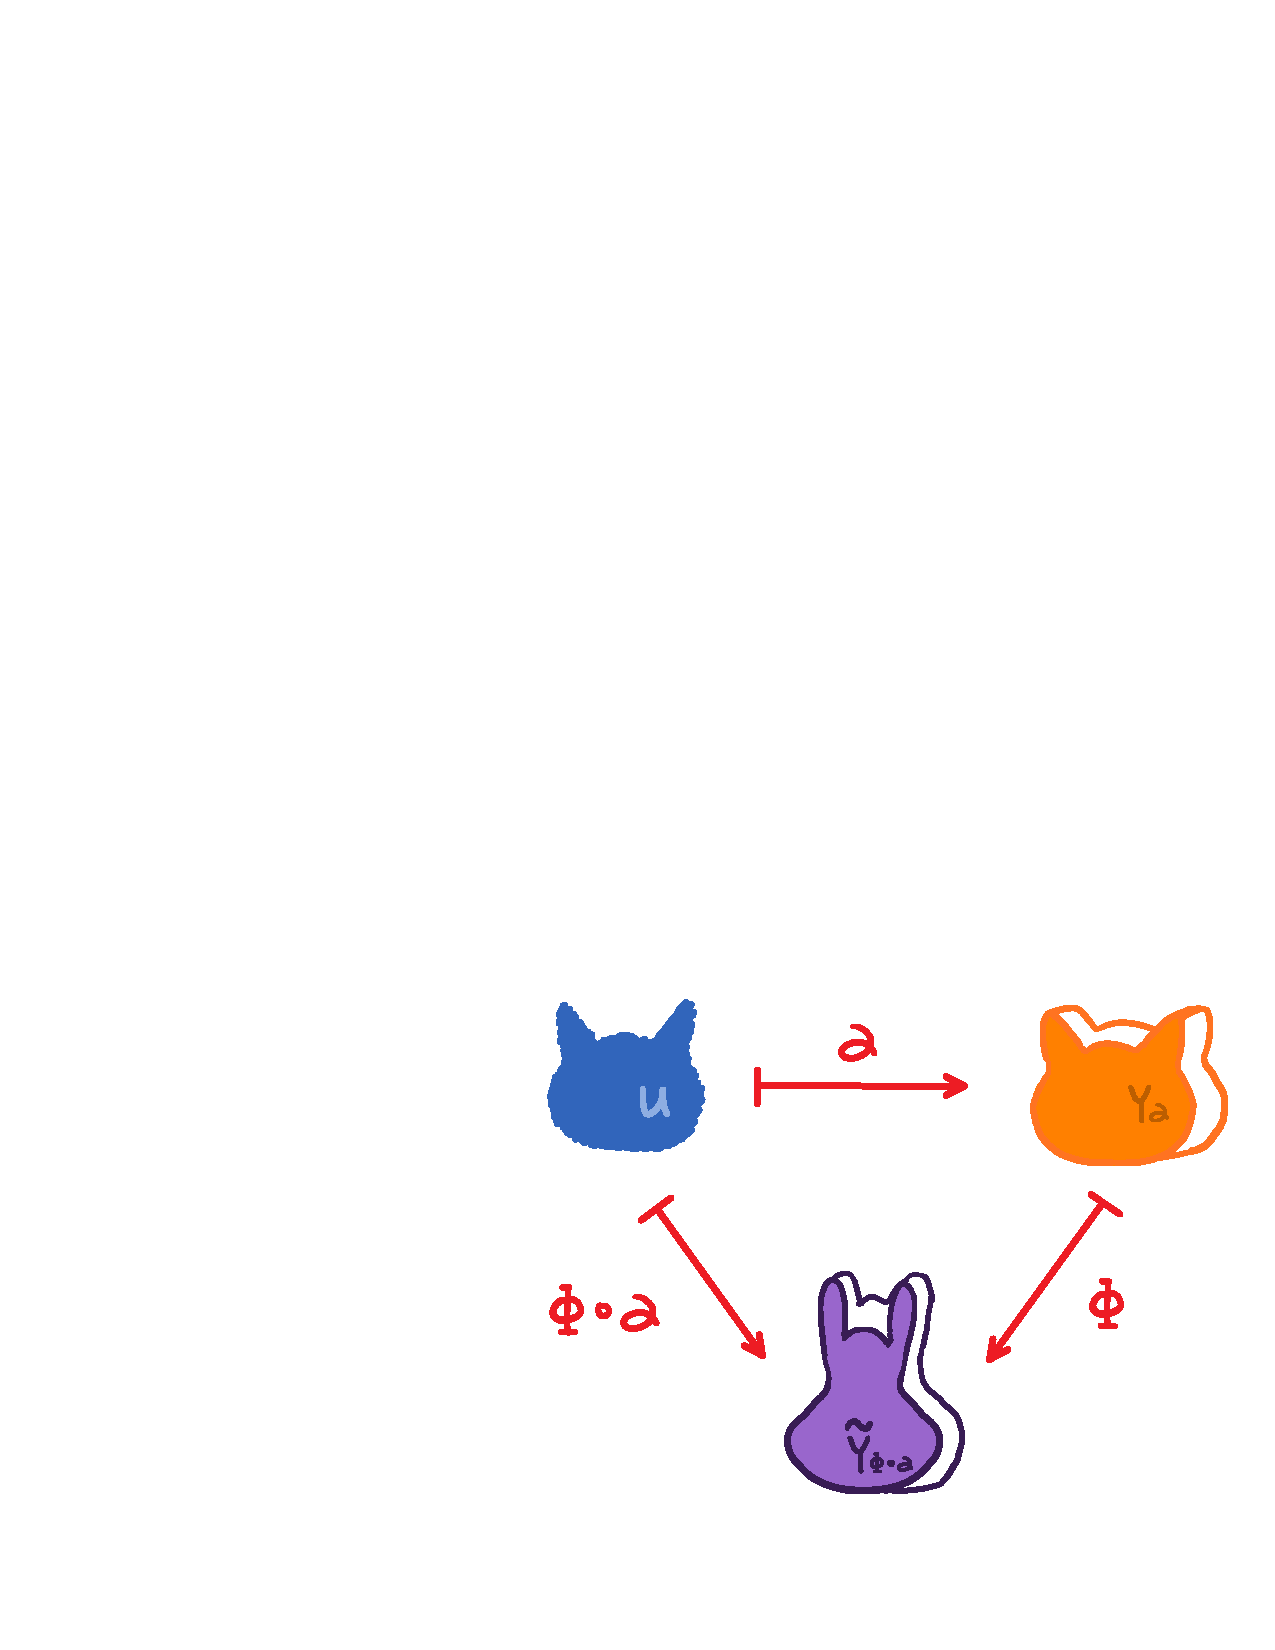
\includegraphics[scale=0.5]{Intkform1.pdf}
\end{center}

Here we can write the following:
\begin{align*}
\int_{\that{Y}_{\Phi \circ \alpha}} = \int_U (\Phi\circ \alpha)^*\omega = \int_U \alpha^*\Phi^*\omega = \int_{Y_\alpha} \Phi^*\omega
\end{align*}


\newpage
\section[Orientations of Manifolds]{\color{red} Orientations of Manifolds\color{black}}
Here we see that the integral of a $k$-form over a parametrized $k$-manifold in $\R^n$, defined by Definition 29.0.0.0.2, is invariant under reparametrization up to a sign difference. That is, if $\alpha$ and $\beta$ are two parametrizations for a $k$-manifold $Y$, with $k$-form defined on an open subset of $\R^n$ containing $Y$, we have the following holds:
\begin{align*}
\int_{Y_\beta} \omega = \pm \int_{Y_\alpha} \omega
\end{align*}
Hence it is natural to discuss the orientation of a manifold to resolve this issue. Intuitively, the orientation on a manifold $M$ is the division of coordinate patches with connected domains into Group A and Group B, determined by the following conditions:\\

\textit{For coordinate patches $\alpha_1$ and $\alpha_2$ of $M$ with $\alpha_2^{-1} \circ \alpha_1$ being well defined: \\
If we have $\det(D(\alpha_2^{-1} \circ \alpha_1))>0$, then $\alpha_1$ and $\alpha_2$ belong to the same group. \\
If we have $\det(D(\alpha_2^{-1} \circ \alpha_1))<0$, then $\alpha_1$ and $\alpha_2$ belong to opposite groups. }\\

We call one of the two groups, say Group A, to be orientation preserving group, and the other to be orientation reversing group. Any coordinate patch in the orientation preserving group is said to be orientation preserving, and any coordinate path in the orientation reversing group is said to be orientation reversing. \\

\exercise Given an oriented $k$-manifold $M $ in $\R^n$, there exists a $k$-form $\omega$ defined on an open subset of $\R^n$ containing $M$ such that, for each point $\vec{p}\in M$ along with a coordinate patch $\alpha_{\vec{p}}$ for $\vec{p}\in M$, $(\alpha_{\vec{p}})^*\omega(\alpha_{\vec{p}}^{-1}(\vec{p}))$ is positive, or negative, multiple of $dx_1\wedge dx_2 \wedge \cdots \wedge dx_k$, for orientation preserving $\alpha_{\vec{p}}$, or orientation reversing $\alpha_{\vec{p}}$, respectively.\\

\begin{defn}
Let $V$ be an $n$-dimensional vector space, let $A = (\vec{a}_1,\vec{a}_2,\cdots, \vec{a}_n)$ be an $n$-tuple of independent vectors in $V$. $A$ is called an $n$-frame in $V$. If $V = \R^n$, $A$ is said to be right-handed provided that:
$$\det\left(\bmat{\vec{a}_1 & \vec{a}_2 & \cdots & \vec{a}_n}\right) > 0$$ 
and $A$ is said to be left-handed provided that we have: 
$$\det\left(\bmat{\vec{a}_1 & \vec{a}_2 & \cdots & \vec{a}_n}\right) < 0$$
\end{defn}

\begin{defn}
The collection of all right-handed frames in $\R^n$ is called an orientation of $\R^n$, and so is the collection of left-handed frames. 
\end{defn}

\begin{defn}
To define the orientation of an $n$-dimensional vector space $V$, one can choose a linear isomorphism $T:\R^n \to V$ and define one orientation of $V$ to consist of all frames of the form: $$(T(\vec{a}_1), T(\vec{a}_2),\cdots, T(\vec{a}_n))$$ 
for which $(\vec{a}_1,\vec{a}_2,\cdots, \vec{a}_n)$ is a right-handed frame in $\R^n$, and the other orientation of $V$ to consist of all such frames for which $(\vec{a}_1, \vec{a}_2,\cdots, \vec{a}_n)$ is left-handed.
\end{defn}

\remark For an $n$-dimensional vector space $V$, from Definition 30.0.0.0.3, we see that $V$ has two orientations, each is called the reverse, or the opposite, of the other. \\

\note It is easy to see that, in the settings of Definition 30.0.0.0.3, the orientation of $V$ is independent of the choice of $T$. Note that in an arbitrary $n$-dimensional vector space, there is no well-defined notion of "right-handed," although there is a well-defined notion of orientation.

\begin{thm}[Theorem 20.3 on Munkres]
Let $C$ be an invertible $n\times n$ matrix, let $h:\R^n \to \R^n \ \ \ \vec{x}\mapsto C\cdot \vec{x}$ be a linear transformation, and let $A=(\vec{a}_1,\vec{a}_2,\cdots, \vec{a}_n)$ be a frame in $\R^n$. If $\det(C) >0$, then the frames $A$ and $H=(h(\vec{a}_1),h(\vec{a}_2),\cdots, h(\vec{a}_n))$ belong to the same orientation of $\R^n$. If $\det(C)<0$, then the frames $A$ and $H$ belong to opposite orientations of $\R^n$.
\end{thm}

\begin{defn}
Let $C$ be an invertible $n\times n$ matrix, let $h:\R^n \to \R^n \ \ \ \vec{x}\mapsto C\cdot \vec{x}$ be a linear transformation. $h$ is said to be orientation preserving provided that $\det(C)>0$. $h$ is said to be orientation reversing provided that $\det(C)<0$. 
\end{defn}

More generally, we can write the following:
\begin{defn}
Let $A,B$ be open subsets of $\R^k$, let $g:A \to B$ be a diffeomorphism, $g$ is said to be orientation preserving provided that $\det(Dg(\vec{x}))>0$ for all $\vec{x}\in A$, and $g$ is said to be orientation-reversing provided that $\det(Dg(\vec{x}))<0$ for all $\vec{x}\in A$. 
\end{defn}

In order for Definition 30.1.0.0.2 to make sense, we here formulate a definition for the tangent spaces, following the notation from Munkres:
\begin{defn}
Let $\vec{x}\in \R^n$. For $\vec{v}\in \R^n$, the pair $(\vec{x};\vec{v})$ is called a tangent vector to $\R^n$ at $\vec{x}$. 
\end{defn}

\begin{defn}
Let $\vec{x}\in \R^n$. For $\vec{v},\vec{w}\in \R^n$, and $c \in \R$, we define:
\begin{align*}
(\vec{x};\vec{v}) + (\vec{x};\vec{w}) = (\vec{x}; \vec{v}+\vec{w})\qquad\qquad\qquad c(\vec{x};\vec{v}) = (\vec{x};c\vec{v})
\end{align*}
The set of all tangent vectors to $\R^n$ at $\vec{x}$ forms a vector space, called the tangent space to $\R^n$ at $\vec{x}$, denoted as $\T_{\vec{x}}(\R^n)$
\end{defn}

\note Although both $\vec{x}$ and $\vec{v}$ given in Definition 30.1.0.0.4 are element of $\R^n$, they play different roles in such definition. One can think of $\vec{x}$ as a point in $\R^n$ and picture it as a dot, think of $\vec{v}$ as an element in $\R^n$ and picture it as an arrow. We picture $(\vec{x};\vec{v})$ as an arrow with its initial point at $\vec{x}$. The set $\T_{\vec{x}}(\R^n)$ is pictured as the set of all arrows with their initial points at $\vec{x}$, which equivalently, can be written as $\{\vec{x}\}\times \R^n$. \\

\note We do not attempt to form the sum $(\vec{x};\vec{v})+(\vec{y};\vec{w})$ for $\vec{x},\vec{y},\vec{v},\vec{w} \in \R^n$ if $\vec{x}\neq \vec{y}$.

\begin{defn}
Let $(a,b)$ be an open interval in $\R$, let $\gamma:(a,B) \to \R^n$ be a function of $C^r$ type. \\
The velocity vector of $\gamma$ at $t \in (a,b)$ is defined to be $(\gamma(t); D\gamma(t))$. 
\end{defn}

\begin{center}
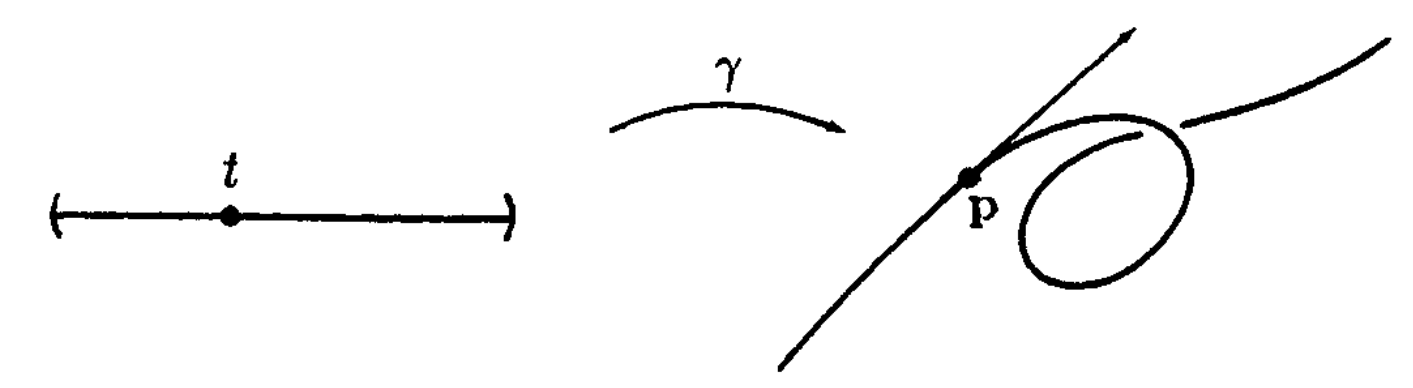
\includegraphics[scale=0.3]{1tangent.png}\\
(Figure 29.1 from Munkres Section 29)
\end{center}

\note In the settings of Definition 30.1.0.0.5, $(\gamma(t); D\gamma(t))$ is viewed as an arrow in $\R^n$ with its initial point at $\vec{p} = \gamma(t)$, pointing towards the direction of motion. \\

\begin{defn}
Let $A$ be a subset of $\R^k$, open in $\R^k$, or in $\mathbb{H}^k$, let $\alpha:A \to \R^n$ be a function of $C^r$ type, let $\vec{x} \in A$, and let $\vec{p} = \alpha(\vec{x})$. We define a linear transformation:
\begin{align*}
\alpha_*: \T_{\vec{x}}(\R^k) \to \T_{\vec{p}}(\R^n) \ \ \ (\vec{x},\vec{v})\mapsto (\vec{p}; D\alpha(\vec{x})\cdot \vec{v})
\end{align*}
$\alpha_*$ is said to be the transformation induced by the differentiable map $\alpha$. 
\end{defn}

\begin{center}
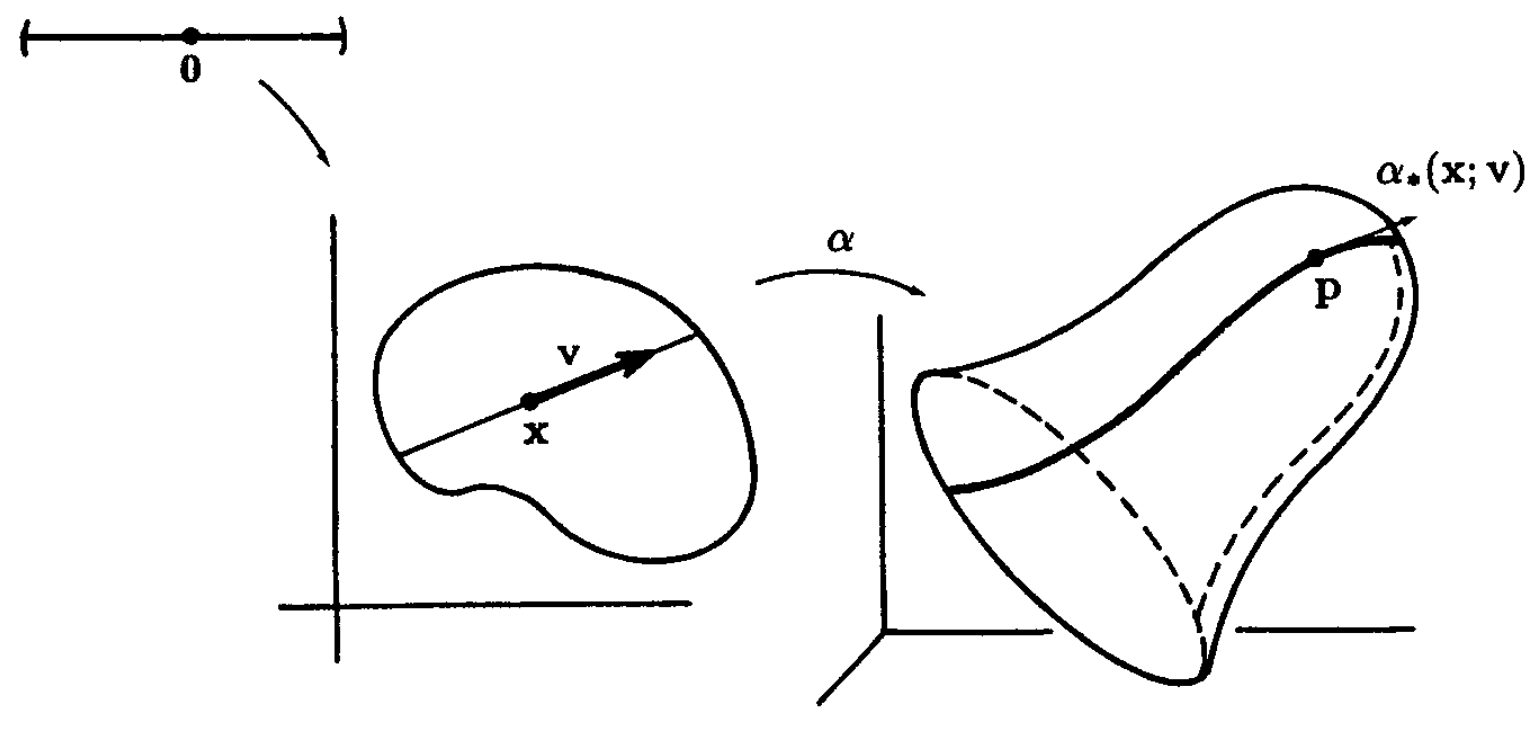
\includegraphics[scale=0.29]{ntangent.png}\\
(Figure 29.2 from Munkres Section 29)
\end{center}

\note Given $(\vec{x}; \vec{v})$ in the definition 30.1.0.0.6, the chain rule implies that the vector $\alpha_*(\vec{x};\vec{v})$ is the velocity vector of the curve $\gamma(t) = \alpha(\vec{x}+t\vec{v})$, corresponding to the parameter value $t = 0$.\\

\note From Lemma 29.1 on Munkres, Let $A,B$ be an subsets of $\R^k$, open in either $R^k$ or in $\mathbb{H}^k$, let $\alpha :A \to R^m$ be a function of of $C^r$ type, with $B$ containing $\alpha(A)$, let $\beta:B \to \R^n$ be a function of $C^r$ type. Then we have $(\beta\circ \alpha)_* = \beta_* \circ \alpha_*$.\\

\begin{defn}
Let $A$ be an open subset of $\R^n$, a tangent vector field in $A$ is a continuous function $F:A \to \R^n \times \R^n$ such that $F(\vec{x}) \in \T_{\vec{x}}(\R^n)$ for each $\vec{x}\in A$. 
\end{defn}

\note In the settings of Definition 30.1.0.0.7, $F$ has the form $F(\vec{x}) = (\vec{x};f(\vec{x}))$ where $f :A \to \R^n$. If $F$ is of $C^r$ type, we say that it is a tangent vector field of $C^r$ type. 

\begin{defn}
Let $M$ be a $k$-manifold of class $C^r$ in $\R^n$, let $\vec{p}\in M$ with a coordinate patch $\alpha: U \to V$ for $\vec{p} \in M$, where $U$ is a subset of $\R^k$, open in either $\R^k$ or $\mathbb{H}^k$, let $\vec{x}\in U$ such that $\alpha(\vec{x})  = \vec{p}$. The set of all vectors of the form $\alpha_*(\vec{x}; \vec{v})$, where $\vec{v}\in \R^k$, is called the tangent space to $M$ at $\vec{p}$, denoted as $\T_{\vec{p}}(M)$. That is, we have $\T_{\vec{p}}(M) = \alpha_*(\T_{\vec{x}}(\R^k))$. 
\end{defn}

\begin{center}
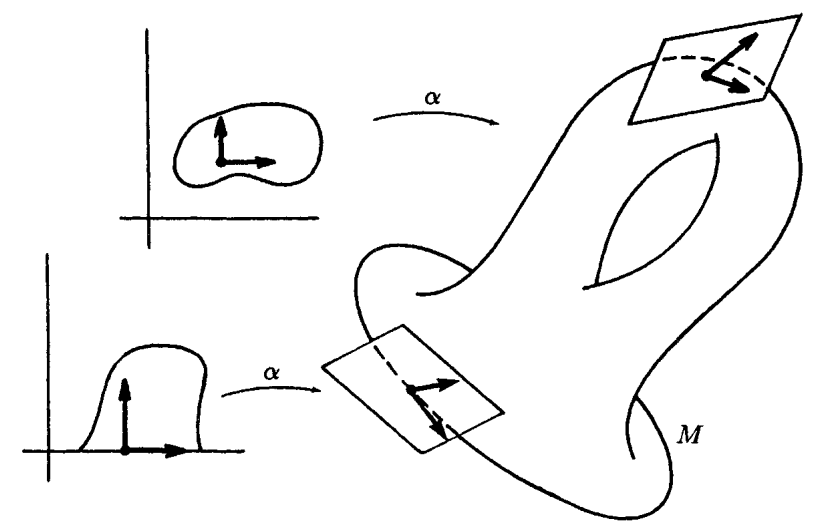
\includegraphics[scale=0.45]{mtangent.png}\\
(Figure 29.3 from Munkres Section 29)
\end{center}

From discussion in section 16 in this text, it is easy to show that $\T_{\vec{p}}(M)$ given in Definition 30.1.0.0.8 is a linear subspace of $\T_{\vec{p}}(\R^n)$ that is well-defined, independent of the choice of $\alpha$. Since $\R^k$ is spanned by the standard basis $\vec{e}_1,\vec{e}_2,\cdots, \vec{e}_k$, the space $\T_{\vec{p}}(M)$ is spanned by the vectors in the family given by:
$$T = \left((\vec{p}\ ;\ D\alpha(\vec{x})\cdot \vec{e}_j ) = \left.\left(\vec{p}\ ;\ \frac{\partial \alpha}{\partial x_j }\right) \right| j \in \N , \ 1\leq j \leq k\right) $$
Since $D\alpha$ has rank $k$, vectors in $T$ are linearly independent, hence they form a basis for the vector space $\T_{\vec{p}}(M)$. \\

Now for the function $g $ defined in Definition 30.1.0.0.3, there is an associated linear transformation of tangent space:
\begin{align*}
g_*: \T_{\vec{x}}(\R^k) \to \T_{g(\vec{x})}(\R^k) \ \ \ (\vec{x};\vec{v}) \mapsto (g(\vec{x}) ; Dg(\vec{x}) \cdot \vec{v})
\end{align*}
Then $g$ is orientation preserving provided that for each $\vec{x}$ in the domain of $g$, the linear transformation of $\R^k$, whose matrix is $Dg$, is orientation-preserving in the sense of Definition 30.1.0.0.1.\\

\begin{defn}
Let $M$ be a $k$-manifold in $\R^n$. Given coordinate path $\alpha_i:U_i \to V_i$ on $M$ for $i = 0,1$, we say $\alpha_1,\alpha_0$ overlap if $V_0 \cap V_1 \neq \emptyset$. We say $\alpha_1,\alpha_0$ overlap positively provided that the transition function $\alpha_1^{-1} \circ \alpha_0$ is orientation preserving.
\end{defn}

\begin{defn}
Let $M$ be a $k$-manifold in $\R^n$. $M$ is said to be orientable provided that $M$ can be covered by a collection of coordinate patches such that each pair of coordinate patches overlap positively, if they overlap at all. $M$ is said to be non-orientable if it cannot be covered by such collection of coordinate patches. 
\end{defn}

\begin{defn}
Let $M$ be an orientable $k$-manifold in $\R^n$. Given a collection of coordinate patches covering $M$ that overlap positively, adjoin to this collection all other coordinate patches on $M$ that overlap these patches positively, denote such collection as $O$. $O$ is called an orientation on $M$. 
\end{defn}

\note In the settings of Definition 30.1.0.0.11, it is easy to see that coordinate patches in $O$ overlap one another positively.

\begin{defn}
A manifold $M$ together with an orientation of $M$ is called an oriented manifold. Given an oriented manifold $M$ along with its orientation $O$, a coordinate patch $\alpha$ on $M$ is said to be orientation preserving provided that $\alpha$ overlaps any one of the coordinate patches in $O$ positively. Otherwise $\alpha$ is said to be orientation reversing. 
\end{defn}

\note If a $k$-manifold $M$ in $\R^n$ is orientable, let $N$ denote the number of connected components of $M$, then $M$ has $2^{N}$ orientations. \\


\newpage
\section[Orientable Manifolds]{\color{red}Orientable Manifolds \color{black}}

First we note that, by the definition of orientable manifold, the discussion makes no sense for a $0$-manifold, which is just a discrete collection of points. A details about orientation of $0$-manifold is discussed in Munkres.\\

In certain dimensions, the notion of orientation of a $k$-manifold has a geometric interpretation that is easily described. This situation occurs when $k = 1$, $k=n-1$, or $k=n$.\\

In the case $k=1$, we can picture an orientation in terms of a tangent vector field, as we proposed in the following definition:
\begin{defn}
Let $M$ be an oriented $1$-manifold in $\R^n$. We define a corresponding unit tangent vector field $\vec{T}$ on $M$ as follows: Given $\vec{p} \in M$, choose a coordinate patch $\alpha_{\vec{p}} :U \to V$ on $M$ about $\vec{p}$ belonging to the given orientation of $M$, and define the following:
\begin{align*}
\vec{T}:M \to \R^n\times \R^n \ \ \ \vec{p}\mapsto \left(\vec{p}\ ;\ \frac{D\alpha_{\vec{p}}(t_0)}{||D\alpha_{\vec{p}}(t_0)||}\right)
\end{align*}
where $t_0$ is the parameter value such that $\alpha_{\vec{p}}(t_0 ) = \vec{p}$. Here $\vec{T}$ is called the unit tangent field corresponding to the orientation of $M$.
\end{defn}

Note that, in the settings of Definition 31.0.0.0.1, $(\vec{p};D\alpha(t_0))$ is the velocity vector of the curve $\alpha$ corresponding to the parameter value $t = t_0$. Then we know that $\vec{T}(\vec{p})$ is such velocity vector divided by its length. \\

In the following we will show that $\vec{T}$ given in Definition 31.0.0.0.1 is well defined.
\begin{proof}
Let $\beta$ be a another coordinate patch on $M$ about $\vec{p}$ belonging to the orientation of $M$, and we denote $\vec{p} = \beta(t_1)$, let $g = \beta^{-1}\circ \alpha$. Then $g$ is a diffeomorphism between an open neighborhood of $t_0$ and an open neighborhood of $t_1$. Here we can write:
\begin{align*}
D\alpha(t_0) = D(\beta \circ g) (t_0) = D\beta(t_1) \cdot Dg(t_0)
\end{align*}
Note that $Dg(t_0)$ is a $1\times 1$ matrix, and since $g$ is orientation preserving, we must have $Dg(t_0) >0$, so we conclude that:
\begin{align*}
\frac{D\alpha(t_0)}{||D\alpha(t_0)||} = \frac{D\beta(t_1)}{||D\beta(t_1)||} 
\end{align*}
The result follows.
\end{proof}

\hfill\break
\example Note that a difficulty arises if a $1$-manifold $M$ has nonempty manifold boundary, in particular, if $\partial M$ contains two distinct points $\vec{p}$ and $\vec{q}$. The coordinate patches for $\vec{p}$ and $\vec{q}$, defined on a subsets of $\mathbb{H}^1$ open in $\mathbb{H}^1$, will induce tangent vectors pointing into $M$ from the two points. 
\begin{center}
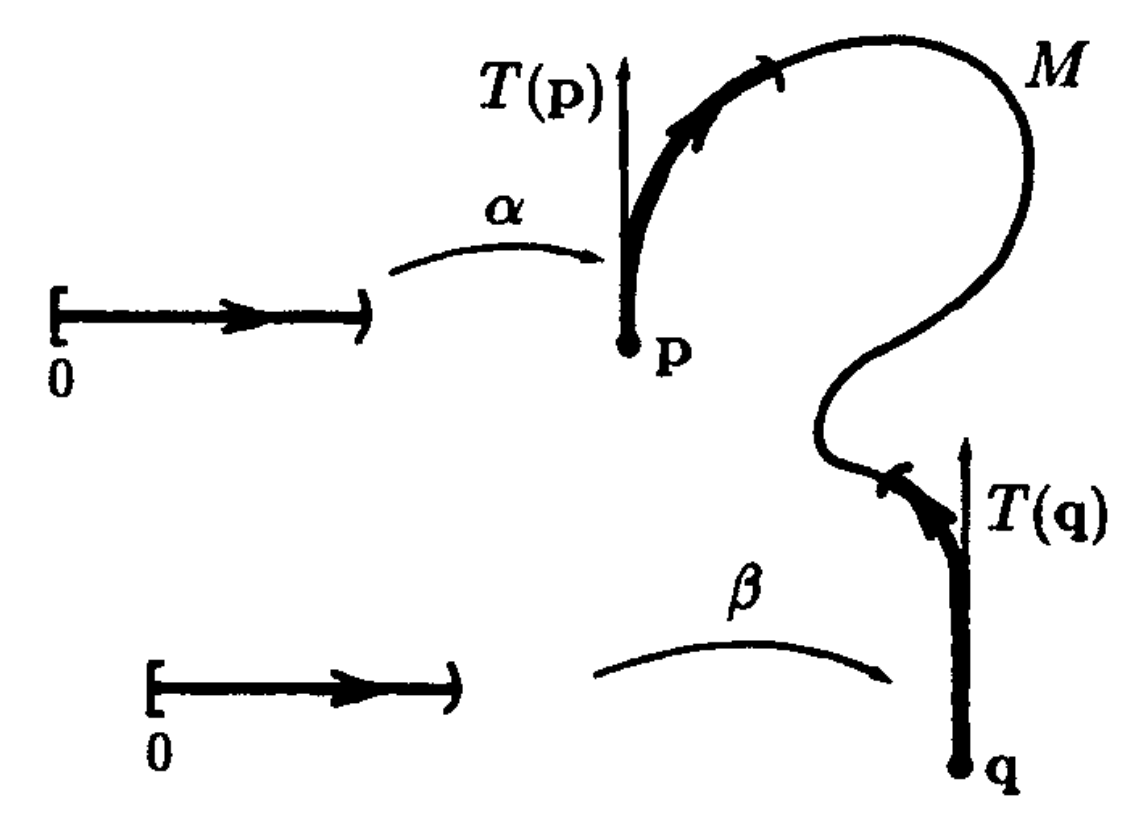
\includegraphics[scale=0.18]{tangent1.png}\qquad\qquad 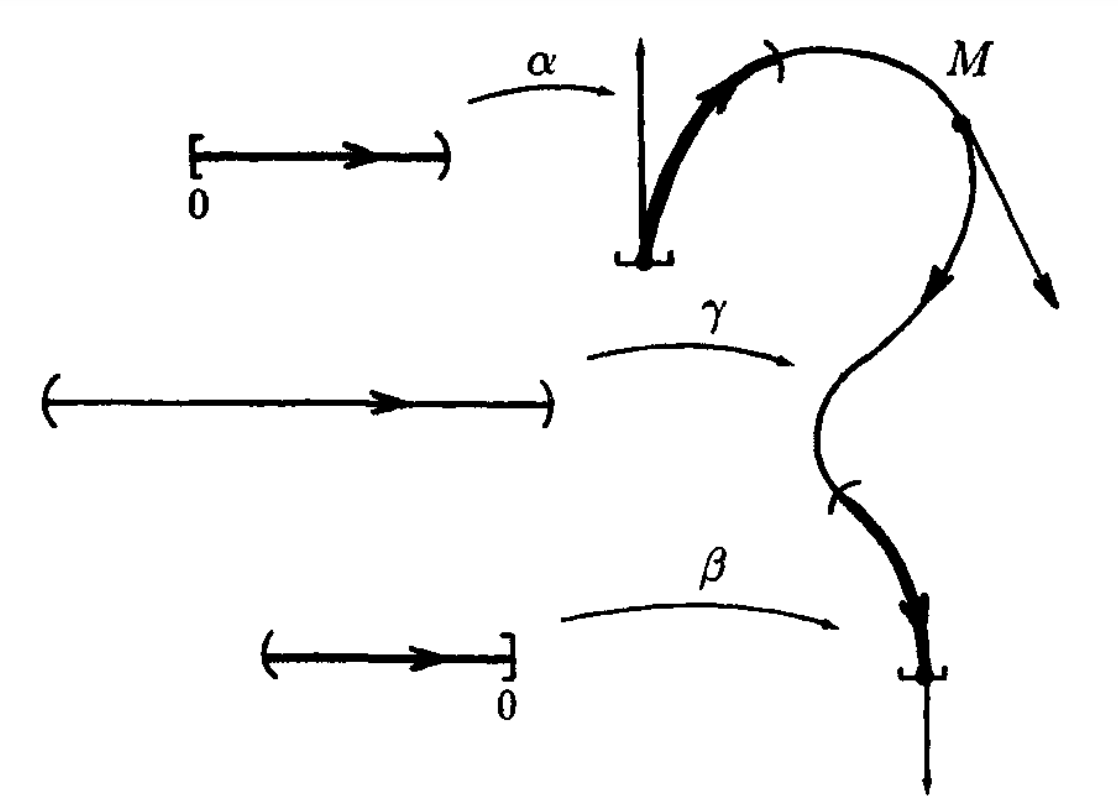
\includegraphics[scale=0.23]{tangent1-1.png}\\
(Figure 34.2 from Munkres Section 34)\qquad\
(Figure 34.3 from Munkres Section 34)\quad
\end{center}
\hfill\break

In the $1$-manifold indicated in the picture, there is no way to define a unit tangent field on $M$ that points into $M$ at both $\vec{p}$ and $\vec{q}$. This problem disappears if we allow our coordinate patches whose domains are open in $\R^1$, or $\mathbb{H}^1$, or in  the left half-line $\mathbb{L}^1 = \{x \mid x\leq 0\}$. With this extra degree of freedom, it is easy to cover the $1$-manifold with two boundary points that overlap positively, and such that the unit tangent field of such manifold is well defined. \\

\note In the case of $1$-manifold $M$, we allow the domains of the coordinate patches on $M$ to be open sets in $\R^1$, $\mathbb{H}^1$, or in $\mathbb{L}^1$, such that every $1$-manifold is orientable.\\

\hfill\break
Now we consider the case where $M$ is an $(n-1)$-manifold in $\R^n$. In this case, we can picture an orientation of $M$ in terms of a unit normal vector field to $M$, as proposed in the following:
\begin{defn}
Let $M$ be an oriented $(n-1)$-manifold in $\R^n$, let $\vec{p} \in M$, let $\alpha:U \to V$ be a coordinate patch on $M$ about $\vec{p}$ belonging to the given orientation of $M$, denote $\alpha(\vec{x}) = \vec{p}$, then the columns $D_i\alpha(\vec{x})$ of the matrix $D\alpha(\vec{x})$ gives basis for $\T_{\vec{p}}(M)$, the tangent space to $M$ at $\vec{p}$. That is, the family of vectors defined by the following defines a basis of $\T_{\vec{p}}(M)$:
\begin{align*}
\left(\left(\vec{p}\ ; D_1\alpha(\vec{x})\right),\ \left(\vec{p}\ ; D_2\alpha(\vec{x})\right),\ \cdots, \left(\vec{p}\ ; D_{n-1}\alpha(\vec{x})\right)\right)
\end{align*}
Let $(\vec{p};\, \vec{n}(\vec{p}))$ be a unit vector in the $n$-dimensional vector space $\T_{\vec{p}}(\R^n)$ that is orthogonal to the $(n-1)$-dimensional linear subspace $\T_{\vec{p}}(M)$. Here $\vec{n}(\vec{p})$ is uniquely determined up to a sign, we specify the sign of $\vec{n}(\vec{p})$ by requiring the frame defined by the following to be right-handed:
\begin{align*}
\left(\vec{n}(\vec{p}),\ D_1\alpha(\vec{x}),\ D_2\alpha(\vec{x}),\ \cdots,\ D_{n-1}\alpha(\vec{x})\right)
\end{align*}
That is, the matrix $\bmat{\vec{n}(\vec{p})& D\alpha(\vec{x})}$ has positive determinant.  The vector field defined by the following is called the unit normal field to $M$ corresponding to the orientation of $M$:
$$\vec{N}:M \mapsto \R^n\times \R^n \ \ \ \ \vec{p}\mapsto (\vec{p};\, \vec{n}(\vec{p}))$$
\end{defn}
 
\example The $2$-manifold Mobius Band in $\R^3$ is not orientable, because it has no continuous unit normal vector field. \\

\example The $2$-manifold Klein Bottle in $\R^4$ is also non-orientable. \\

Now we consider the case where $M$ is an $n$-manifold in $\R^n$. In this case, $M$ is always orientable, and it also has a natural orientation, as a proposed in the following definition:
\begin{defn}
Let $M$ be an $n$-manifold in $\R^n$. The natural orientation of $M$ consists of all coordinate patches $\alpha$ on $M$ for which $\det(D\alpha(\vec{x})) >0$ for all $\vec{x}$ in the definition of domain of $\alpha$. 
\end{defn}

\begin{prop} All $n$-manifolds in $\R^n$ are orientable. 
\end{prop}
\begin{proof}
Let $\vec{p}\in M$, let $\alpha:U \to V$ be a coordinate patch on $M$ about $\vec{p}$. Here we note that $U$ is either open in $\R^n$ or open in $\mathbb{H}^n$, by shrinking $U$ if necessary, we can assume that $U$ is either an open ball, or the intersection of an open ball with $\mathbb{H}^n$. In either case, we know that $U$ is connected, so $\det(D\alpha(\vec{x}))$ is either all positive, or all negative, for all $\vec{x}\in U$. If the former, then $\alpha$ is our desired coordinate patch about $\vec{p}$. If the later, then $\alpha\circ r$ is our desired coordinate patch about $\vec{p}$, where $r$ is defined by $r:\R^n \to \R^n \ \ \ (x_1,x_2,\cdots, x_n) \mapsto (-x_1,x_2,\cdots, x_n)$. Since $\vec{p}$ is arbitrary, this completes the proof. 
\end{proof}

\begin{defn}
Let $r:\R^k \to \R^k \ \ \ (x_1,x_2,\cdots, x_n) \mapsto (-x_1,x_2,\cdots, x_n)$ be the reflection map, let $M$ be an oriented $k$-manifold in $\R^n$. For each coordinate patch on $M$, $\alpha_i :U_i \to V_i$, that belongs to the orientation of $M$, let $\beta_i $ be the coordinate patch on $M$ defined by:
\begin{align*}
\beta_i : r(U_i) \to V_i \ \ \ \ \vec{x}\mapsto (\alpha_i \circ r)(\vec{x})
\end{align*}
The set of all such $\beta_i$ is called the reverse, or opposite, orientation to the orientation of $M$ specified by the the coordinate patches $\alpha_i$
\end{defn}

\note In the settings of the Definition 31.0.1.0.1, $\beta_i$ does not overlap $\alpha_i$ positively, so $\beta_i$ does not belong to the orientation of $M$ specified by the set of coordinate patches that contains $\alpha_i$. By the definition, $\beta_i$ overlap each other positively. \\


\note The reflection map $r$ defined in Definition 31.0.1.0.1 is it s own inverse. $r$ carries $\mathbb{H}^k$ to $\mathbb{H}^k$ if $k>1$, and it carries $\mathbb{H}^1$ to $\mathbb{L}^1$. \\

\note Now it follows that every orientable $k$-manifold $M$ has at least two orientations, a given one and its opposite. If $M$ is connected, it has only two orientations, and otherwise it has more than two. \\

\note If $M$ is an oriented $1$-manifold with corresponding tangent field $\vec{T}$, then reversing the orientation of $M$ induces the corresponding tangent field $-\vec{T}$.\\

\note If $M$ is an $n-1$ manifold in $\R^n$ with corresponding normal field $\vec{N}$, reversing the orientation of $M$ induces the corresponding normal field $-\vec{N}$. \\
\newpage

\begin{thm}[Theorem 34.1 on Munkres]
Let $k>1$, let $M$ be an orientable $k$-manifold with non-empty boundary. \\
$\partial M$ is orientable.
\end{thm}
\begin{proof}
Let $\vec{p} \in \partial M$, and let $\alpha:U \to V$ be a coordinate patch on $M$ about $\vec{p}$ belonging to a given orientation of $M$. Here we define:
\begin{align*}
b:\R^{k-1}\to \R^k \ \ \ \ (x_1,x_2,\cdots, x_{k-1}) \mapsto (x_1,x_2,\cdots, x_{k-1},0)
\end{align*}
The function $\alpha_0 \coloneqq \alpha\circ b$ defines a coordinate patch on $\partial M$ about $\vec{p}$. Here $\alpha_0$ is said to be obtained by restricting $\alpha$. Theorem 34.1 on Munkres shows in details that the set of such coordinate patches $\alpha_0$ on $\partial M$, obtained by restricting coordinate patches $\alpha$ on $M$ in the given orientation of $M$, constitutes an orientation of $\partial M$. 
\end{proof}

\hfill\break
\hfill\break
Theorem 31.1 shows that, given an orientation of a $k$-manifold $M$ that has nonempty boundary, one can obtain an orientation of $\partial M$ by simply taking restrictions of coordinate patches that belong to the orientation of $M$. However, this orientation of $\partial M$ is not always the one we prefer. Here we propose the following definition:
\begin{defn}
Let $M$ be an orientable $k$-manifold with nonempty manifold boundary $\partial M$. Given an orientation $O$ of $M$, the corresponding induced orientation of $\partial M$ is defined as follows:
\begin{enumerate}[topsep=3pt,itemsep=-1ex,partopsep=1ex,parsep=1ex]
\item If $k$ is even, the corresponding induced orientation of $\partial M$ is the orientation obtained by restricting coordinate patches belonging to $O$.
\item If $k$ is odd, the corresponding induced orientation of $\partial M$ is the opposite of the orientation of $\partial M$ obtained by restricting coordinate patches belonging to $O$.
\end{enumerate}
\end{defn}

\example \\
Let $M$ be a naturally oriented $3$-manifold in $\R^3$ with nonempty boundary, and let $\vec{p}\in \partial M$ with coordinate patch $\alpha: U \to V$ on $M$ about $\vec{p}$ belonging to the orientation of $M$. Since $M$ is naturally oriented, then we can write, with $\alpha(\vec{q}) = \vec{p}$:
\begin{align*}
\det(D\alpha(\vec{q})) 
&=\det \left(\bmat{D_1\alpha(\vec{q}) & D_2\alpha(\vec{q})& D_3\alpha(\vec{q})}\right) \\
&=\det \left(\bmat{D_3\alpha(\vec{q}) & D_1\alpha(\vec{q})& D_2\alpha(\vec{q})}\right)>0
\end{align*}
so we know that the frame $( D_3\alpha(\vec{q}),\ D_1\alpha(\vec{q}),\ D_2\alpha(\vec{q}))$ is right-handed. Restricting $\alpha$ in the orientation of $M$, we get an orientation of $\partial M$, but the induced orientation of $\partial M$ induced by the orientation of $M$ is, by definition, taken to be to opposite of the orientation of $\partial M$ obtained by restricting $\alpha$. Thus the normal field at point $\vec{p}$, denoted as $\vec{N}(\vec{p}) = (\vec{p}; \vec{n}(\vec{p}))$,  corresponding to the induced orientation of $\partial M$ satisfies the following condition:
\begin{align*}
\text{The frame }\left(-\vec{n}(\vec{p}),\ D_1\alpha(\vec{q}), \ D_2\alpha(\vec{q}) \right) \text{ is right-handed}
\end{align*}
Here we notice that $D_3\alpha(\vec{q})$, by definition, must points into $M$, and hence $-\vec{n}(\vec{p})$ points into $M$. Then we know that $\vec{n}(\vec{p})$, which is the unit normal vector at point $\vec{p}$ specified by the induced orientation of $\partial M$ by the orientation of $M$, points outward from $M$. One might denote $D_1\alpha(\vec{q}), D_2\alpha(\vec{q}), D_3\alpha(\vec{q})$ as $\frac{\partial \alpha}{\partial x_1},\ \frac{\partial \alpha}{\partial x_2},\ \frac{\partial \alpha}{\partial x_1}$ respectively.

\begin{center}
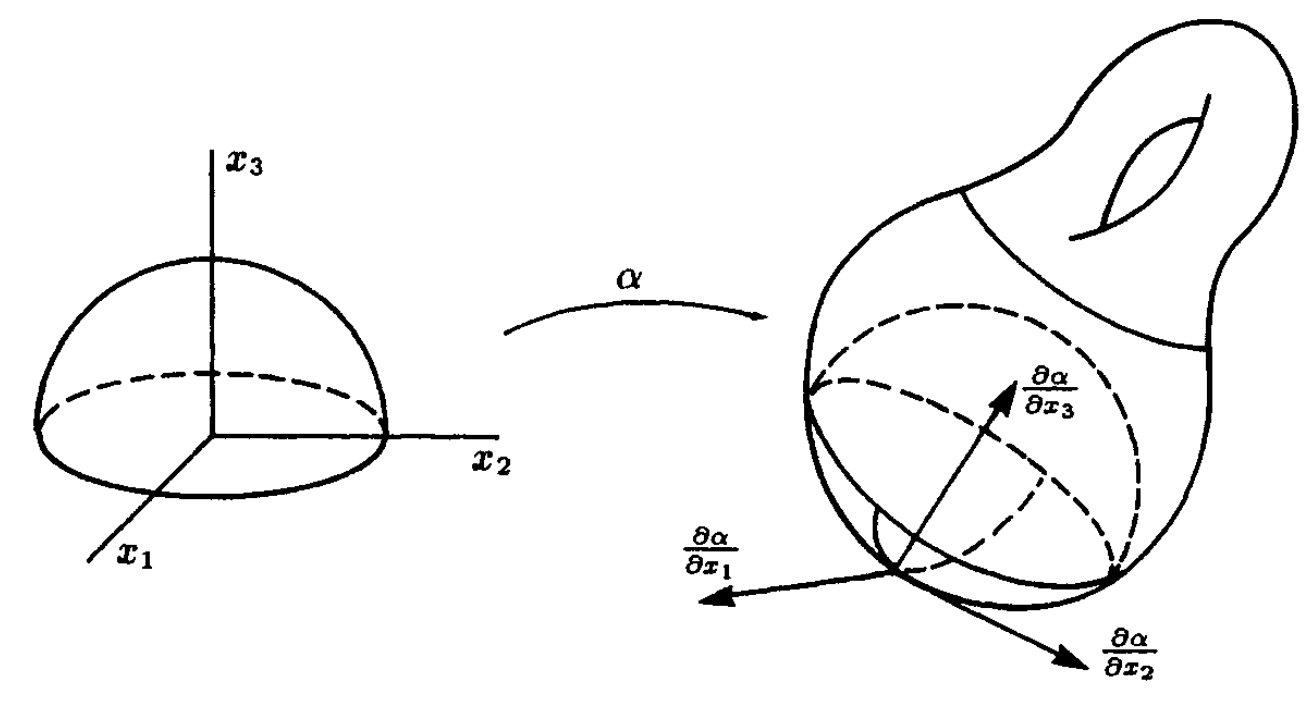
\includegraphics[scale=0.29]{3Orientation.png}\\
(Figure 34.9 from Munkres Section 34)
\end{center}

\example \\
Now let $M$ be an oriented $2$-manifold with nonempty boundary in $\R^3$, and give $partial M$ the induced orientation. Let $\vec{N}$ be the unit normal field to $M$ corresponding to the orientation of $M$, and let $\vec{T}$ be the unit tangent field to $\partial M$ corresponding to the induced orientation of $\partial M$. Note that given a coordinate patch on $M$ about a point $\vec{p} \in \partial M$, with $\alpha(\vec{q}) = \vec{p}$, we note that $D_1\alpha(\vec{q})$ represents the velocity vector of the parametrized curve $\alpha\circ b$ where $b$ is the function defined in Theorem 31.1, hence by definition it points in the same direction as the unit tangent vector $\vec{T}$. On the other hand, $D_2\alpha(\vec{q})$ points in the direction into $M$ from $\partial M$ by definition. Let $\vec{n}(\vec{p})$ be the unit normal vector at point $\vec{p} \in \partial M$, one can compute that: 
$$\det\left(\bmat{\vec{n}(\vec{p})& D_1\alpha(\vec{q})& D_2\alpha(\vec{q})}\right) > 0$$ 

\remark Now let $M$ be an oriented $2$-manifold with nonempty boundary in $\R^3$, and give $partial M$ the induced orientation. Let $\vec{N}$ be the unit normal field to $M$ corresponding to the orientation of $M$, and let $\vec{T}$ be the unit tangent field to $\partial M$ corresponding to the induced orientation of $\partial M$. Informally speaking, the relation between $\vec{N}$ and $\vec{T}$ is such that if one walks around $\partial M$ in the direction specified by $\vec{T}$, with his head pointing in the direction specified by $\vec{N}$, then the manifold $M$ is on his left, in the direction given by a vector $\vec{W}$ orthogonal to both $\vec{T}$ and $\vec{N}$. \\
\begin{center}
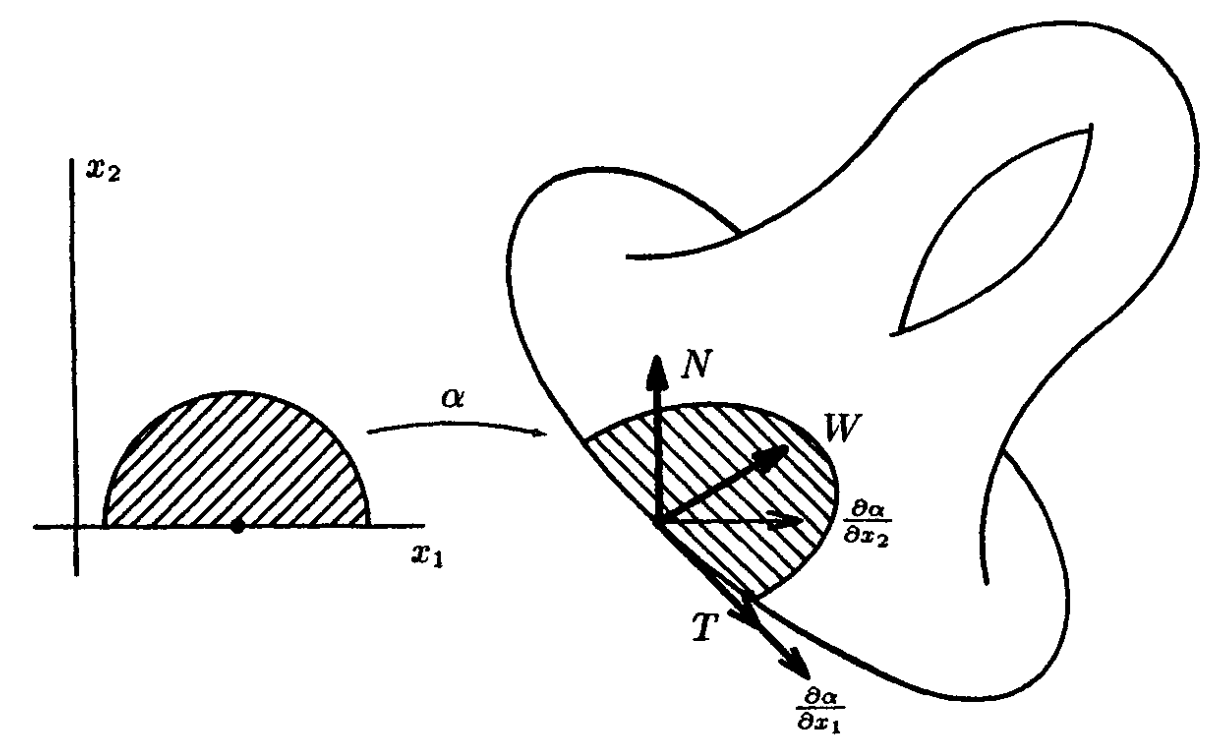
\includegraphics[scale=0.29]{2Orientation.png}\\
(Figure 34.10 from Munkres Section 34)
\end{center}

\hfill\break\hfill\break
Now let $X$ be an oriented $(n-1)$-manifold in $\R^n$, and suppose further that $X$ is the boundary of a $n$-manifold $M$. Let $\alpha$ be a coordinate patch on $X$ belonging to the given orientation of $X$, the tangent space of $X$ at $\vec{p}$, denoted as $\T_{\vec{p}}(X)$ is given by the column space of $D\alpha(\vec{q})$, here $\dim(\T_{\vec{p}}(X)) = n-1$, and $\dim((\T_{\vec{p}}(X))^{\perp}) = 1$. Notice that, here we can define: 
$$\mathcal{N}_{\vec{p}}(X) \coloneqq (\T_{\vec{p}}(X))^\perp$$ 
Here we can pick $\vec{N}(\vec{p}) \in \mathcal{N}_{\vec{p}}(X)$ such that $||\vec{N}(\vec{p})|| = 1$ and the following holds: 
$$\det\left(\bmat{\vec{N}(\vec{p}) & D\alpha(\vec{q})}\right) >0$$ 
Define $\vec{N}:X \to \R^n$ such that $\vec{N}(\vec{p}) \perp \vec{t}$ for all $\vec{t}\in \T_{\vec{p}}(X)$, and such that $||\vec{N}(\vec{p})|| = 1$. Here we note that, such definition of the unit normal field $\vec{N}$ on $X$ corresponding to the given orientation of $X$ is consistent with the definition of normal field given in Definition 31.0.0.0.2. \\

\exercise Let $X$ be an orientable $(n-1)$-manifold in $\R^n$, the definition of the unit normal field $\vec{N}$ on $X$ does not depend on the choice of coordinate patch up to the orientation of $X$ which the coordinate patch belongs to.\\ 

\exercise (Munkres Corollary 38.4)\\
If $X$ is an $(n-1)$-manifold in $\R^n$ of class $C^r$, then $\vec{N} \in C^{r-1}(X, \R^n)$. \\

\exercise For special case where $n$-manifold $M= \mathbb{H}^n$ in $\R^n$, we have $X = \pd M = \R^{n-1}\times \{0\}$, and we have the unit normal field on $X$ has the property that $\vec{N}(\vec{p}) = -\vec{e}_n$, where $\vec{e}_n$ is the last vector in the standard basis of $\R^n$. \\

\exercise Let $M$ be an oriented $n$-manifold in $\R^n$ with nonempty boundary $X = \pd M$. Given the induced orientation of $\partial M$, the unit normal field on $X$ at each point, $\vec{N}(\vec{p})$, points outwards from $X$, that is, we have $\vec{p} + t\vec{N}(\vec{p}) \notin M$ for $0<t<\epsilon$ with some $\epsilon>0$. \\

Conversely, given a unit normal vector field $\vec{N}$ for an orientable $(n-1)$-manifold $X$ in $\R^n$, one can use the sign of following the determinant as a criteria to test the orientation of a coordinate patch $\alpha$ on $X$, or define the orientation of $X$:
$$\det\left(\bmat{\vec{N}(\vec{p})  & D\alpha(\vec{q})}\right)$$ 

Given an orientable $(n-1)$-manifold $X$ and a vector field $v:X \to \R^{n}$ such that $v(\vec{x}) \notin \T_{\vec{p}}(X)$, we obtain an orientation on $X$ by declaring that each coordinate patch $\alpha:U \to V $ on $X$ is orientation preserving provided that the following holds with $\vec{q } = \alpha^{-1}(\vec{p})$: $$\det\left(\bmat{v(\vec{p}) &D\alpha(\vec{q})}\right) >0$$

The orientation of a $1$-manifold $M$ is equivalent to the choice of continuous forward pointing motion $\vec{T}$ along the tangent space of $M$, here $\vec{T}$ is the unit tangent field as we defined above. For $2$-manifold $M $ in $\R^2$, let $X = \pd M$, we get the following for $\vec{p}\in X$:
$$\vec{N}(\vec{p}) = \bmat{0&1 \\ -1 & 0}\vec{T}(\vec{p})$$

In this sense of orientable manifolds, the orientation of $0$-manifold can be defined with the direction of traveling towards the positive and away from the negative.\\

\begin{defn}
Let $M$ be an oriented $k$-manifold in $\R^n$, let $\alpha: U \to V$ be a coordinate patch on $M$ belonging to the given orientation, with $\alpha(\vec{q}) = \vec{p} \in M$, let $\omega$ be a $k$-form defined on an open subset of $\R^n$ containing $M$. We can write $\alpha^*\omega = f(\vec{x}) \, dx_1 \wedge dx_2 \wedge \cdots \wedge dx_k$ for some $0$-form $f$ defined on the definition of domain of $\omega$. $\omega$ is said to be positive for $M$ at $\vec{p}$ provided that $f(\vec{a})>0$, $\omega$ is said to be negative for $M$ at $\vec{p}$ provided that $f(\vec{a})<0$, and $\omega$ is said to be integral for $M$ at $\vec{p}$ provided that $f(\vec{a})=0$.
\end{defn}

\exercise In the settings of Definition 31.1.0.0.2, $\omega$ is integral at $\vec{p}$ if and only if we have:
\begin{align*}
\omega(\vec{p}) (\vec{v}_1,\vec{v}_2,\cdots, \vec{v}_k) = 0\qquad \forall \vec{v}_1,\vec{v}_2,\cdots, \vec{v}_k \in \T_{\vec{p}}(M) 
\end{align*} 

\exercise Let $\alpha$ and $\beta$ be $0$-form defined on $\R^2$. $\alpha\, dx + \beta \, dy$ is integral for the $1$-manifold $\R\times \{0\}$ in $\R^2$ at $\vec{0}$ if and only if we have $\alpha(0,0) = 0$.\\

\begin{defn}
$M$ is integral manifold for $\omega$ provided that $\omega$ is integral for $M$ at $\vec{p}$ for all $\vec{p}\in M$. 
\end{defn}

\exercise If $M$ is an oriented $k$-manifold, then there exists an $k$-form $\omega$ being positive for $M$ at all $\vec{p} \in M$. Conversely, given an $k$-form $\omega$ that is nowhere integral on $M$, there is a unique orientation of $M$ such that $\omega$ is positive for $M$ at all $\vec{p}\in M$.\\

\begin{thm}[Theorem 36.2 on Munkres]
Let $M$ be a compact oriented $k$-manifold in $\R^n$, let $\omega$ be a $k$-form defined in a open subset of $\R^n$ containing $M$, and let $\lambda$ be the scalar function on $M$ defined by the following:
\begin{align*}
\lambda:M \to \R \qquad \vec{p}\mapsto \omega(\vec{p})((\vec{p};\vec{a}_1),(\vec{p};\vec{a}_2),\cdots, (\vec{p};\vec{a}_k))
\end{align*}
where, for $\vec{p}\in M$, the family $((\vec{p};\vec{a}_1),(\vec{p};\vec{a}_2),\cdots, (\vec{p};\vec{a}_k))$ forms an orthonormal frame in the linear space $\T_{\vec{p}}(M)$ belonging to the given orientation of $M$. Then $\lambda$ is continuous, and we have:
\begin{align*}
\int_M \omega = \int_M \lambda \, dV
\end{align*}
\end{thm}
\begin{proof}
A general proof is given in Theorem 36.2 on Munkres. \\
For the case where $k=1$, we can show the following holds:
\begin{align*}
\int_M \omega = \int_M \omega\cdot \vec{T} \, dV
\end{align*}
here $\vec{T}$ is the unit tangent field corresponding to the orientation of $M$.
\end{proof}

\note One can use Theorem 31.2 to define the extended integral $ext\int_M \omega$ for integrating $k$-form over oriented $k$-manifold $M$ in $\R^n$.


\begin{defn}
Let $M$ be an $n$-manifold in $\R^n$ with nonempty manifold boundary. The inward normal to $\partial M$ at $\vec{p}\in \partial M$ is the velocity vector of a curve that begins at $\vec{p}$ and moves into $M$ as parameter value increases, the outward normal is the negative velocity vector of a curve that begins at $\vec{p}$ and moves into $M$ as parameter value increases.
\end{defn}

\begin{lem}[Lemma 38.7 on Munkres]
Let $M$ be an orientable $n$-manifold in $\R^n$. If $M$ is oriented naturally, then the induced orientation of $\partial M$ corresponds to the unit normal field $\vec{N}$ to $\partial M$ that points outwards from $M$ at all $\vec{p}\in \partial M$. 
\end{lem}
\begin{proof}
Let $\vec{p}\in \partial M$, let $\alpha:U \to V$ be a coordinate patch on $M$ about $\vec{p}$ belonging to the orientation of $M$, such that $\alpha(\vec{q}) = \vec{p}$. Here $\alpha_0 = \alpha\circ b$ is a coordinate patch on $\partial M$ about $\vec{p}$, which belongs to the induced orientation of $\partial M$ if $n$ is even, and to the opposite if $n$ is odd, with the function $b$ as defined in Theorem 31.1. Let $\vec{N}$ be the unit normal field to $\partial M$ corresponding to the induced orientation of $\partial M$, denote $\vec{N}(\vec{p}) = (\vec{p};\,\vec{n}(\vec{p}))$, here we can write:
\begin{align*}
\det\left(\bmat{(-1)^n\vec{n}(\vec{p}) & D\alpha_0} \right) > 0 
\quad\Rightarrow\quad  0>\det\left(\bmat{D\alpha_0& \vec{n}(\vec{p})} \right)=-\det\left(\bmat{D\alpha_0& D_{n}\alpha(\vec{q})} \right)   
\end{align*}
$D_n\alpha(\vec{q})$ is the velocity vector of a curve that begins at $\vec{p}$ moving into $M$, hence it follows that $\vec{n}(\vec{p})$ is the outward normal to $\partial M$ at $\vec{p}$. The result follows.
\end{proof}

\newpage
\section[The Generalized Stokes' Theorem]{\color{red}The Generalized Stokes' Theorem\color{black}}
\begin{lem}[Lemma 25.2 on Munkres]
Let $M$ be a compact $k$-manifold in $\R^n$ of class $C^r$. Given a covering $\mathcal{C}$ of $M$ by coordinate patches, there exists a finite collection of $C^\infty$ functions from $\R^n$ to $\R$, denoted as $P = \{ \phi_1, \phi_2,\cdots, \phi_l\}$, such that the followings hold:
\begin{enumerate}[topsep=3pt,itemsep=-1ex,partopsep=1ex,parsep=1ex]
\item For each $1\leq i\leq l$, $\phi_i$ has compact support and there exists a coordinate patch $\alpha_i : U_i \to V_i$ in the collection $\C$ such that we have $\text{supp}(\phi_i) \cap M \subseteq V_i$
\item $\phi_i(\vec{x})\geq 0$ for all $\vec{x} \in \R^n$
\item $\sum_{i=1}^l \phi_i(\vec{x}) = 1$ for all $\vec{x}\in M$
\end{enumerate}
\end{lem}

\note In the settings of Lemma 32.0.1, the collection $P = \{ \phi_1, \phi_2,\cdots, \phi_l\}$ is called a partition of unity on $M$ dominated by the collection $\C$ of the coordinate patches.\\

Let $M$ be a compact oriented $k$-manifold in $\R^n$, along with the orientation $O$, let $\omega$ be a $k$-form defined in an open subset of $\R^n$ containing $M$, let $C = M \cap \text{supp}(\omega)$. Here we see that $C$ is compact because both $M$ and $\text{supp}(\omega)$ are compact. Suppose there exists a coordinate patch $\alpha:U \to V$ on $M$ belonging to the orientation $O$ such that $C \subseteq V$. By replacing $U$ by a smaller open set if necessary, we can assume that $U$ is bounded, and here we define the integral of $\omega$ over $M$ by:
\begin{align*}
\int_M \omega \coloneqq \int_{\text{Int}(U)}\alpha^*\omega \tag{KM}
\end{align*}
Here we note that $U = \text{Int}(U)$ if $U$ is open in $\R^k$, and $\text{Int}(U) = U \cap \mathbb{H}_+^k$ if $U$ is open in $\mathbb{H}^k$.\\

We note that the integral defined by equation (KM) is linear. More precisely, if $k$-forms $\omega$ and $\eta$ have supports whose intersections with $M$ can be covered by the single coordinate patch $\alpha:U \to V$ belonging to $O$, then we can write:
\begin{align*}
\int_M a\omega+ b \eta =\left( a \int_M \omega\right) + \left(b \int_M \eta\right)
\end{align*}
where $a,b \in \R$. We also note that, if $-M$ denotes the manifold $M$ with the opposite orientation, then, given that all appropriate conditions in the discussion above hold, we have the following:
\begin{align*}
\int_{-M}\omega  = -\int_M \omega
\end{align*}

To define $\int_M \omega$ in general, we need to make use of a partition of unity:

\begin{defn}
Let $M$ be a compact oriented $k$-manifold in $\R^n$, along with orientation $O$ on $M$. Cover $M$ by a collection $\C$ of coordinate patches in $O$, then choose a partition of unity $\phi_{1},\phi_2,\cdots, \phi_l$ on $M$ that is dominated by the collection $\C$. Let $\omega$ be a $k$-form defined in an open neighborhood of $M$. We define the integral of $\omega$ over $M$ by the following:
\begin{align*}
\int_M \omega = \sum_{i=1}^l\left( \int_M\phi_i\, \omega\right)
\end{align*}
Equivalently, since $M$ is compact, then we can cover $M$ by finitely many coordinate patches, that is, we can take $\C$ to be a finite collection of coordinate patches in $O$, denoted as $C = \{ \alpha_1, \alpha_2,\cdots, \alpha_N\}$. One can use partition of unity to write $\omega = \sum_{j=1}^N\omega_j $ such that the support of each $\omega_j$ is a subset of $V_j$, where $V_j$ is the codomain of a coordinate patch $\alpha_j: U_j \to V_j$ in $C$. Here we define: 
\begin{align*}
\int_M \omega = \sum_{j=1}^N \left(\int_{(V_j)_{\alpha_j}}\omega_j \right)
\end{align*}
\end{defn}

\note In the settings of Definition 32.0.1.0.1, let $c \in \R$, $\omega_m$ and $\omega_n$ be $k$-forms defined in an open set in $\R^n$ containing $M$, we have immediately that the following holds:
\begin{align*}
\int_M c \omega = c \int_M \omega \qquad\qquad\qquad \int_M(\omega_1+\omega_2) = \int_M \omega_1 + \int_M \omega_2
\end{align*}


\remark Let $U$ be an open subset of $\R^k$, and let $V$ be a $k$-manifold in $\R^n$, let $\alpha:U \to V$ be a orientation preserving coordinate patch for $V$, and let $\beta \coloneqq \alpha^{-1}$. Here $\beta$ is called a chart. For $g :V \to \R$, we can write the following:
\begin{align*}
\int_{V_\alpha} g\, d\beta_1 \wedge d\beta_2 \wedge\cdots \wedge d\beta_k = \int_U (g\circ \alpha)\, dx_1\wedge dx_2 \wedge \cdots \wedge dx_k
\end{align*}

Intuitively, the integral $\int_M dx\wedge dy$ of a $2$-manifold $M$ in $\R^3$ is the projection area of $M$ on the $xy$-plane. Similarly, $\int_M dy\wedge dz$ is the projection area of $M$ on the $yz$-plane, and  $\int_M dx\wedge dz$ is the projection area of $M$ on the $xz$-plane. Note that the orientation of the manifold $M$ would affect the projection area, some of the regions would cancel each other due to the opposite sign specified the orientation.\\
 
\example\\
Consider such chef hat as a $2$-manifold $H$ in $\R^3$, and suppose the bottom of the chef hat, which is the manifold boundary of $H$, is a circle of radius $1$ lies on the $xy$-plane. 
\begin{center}
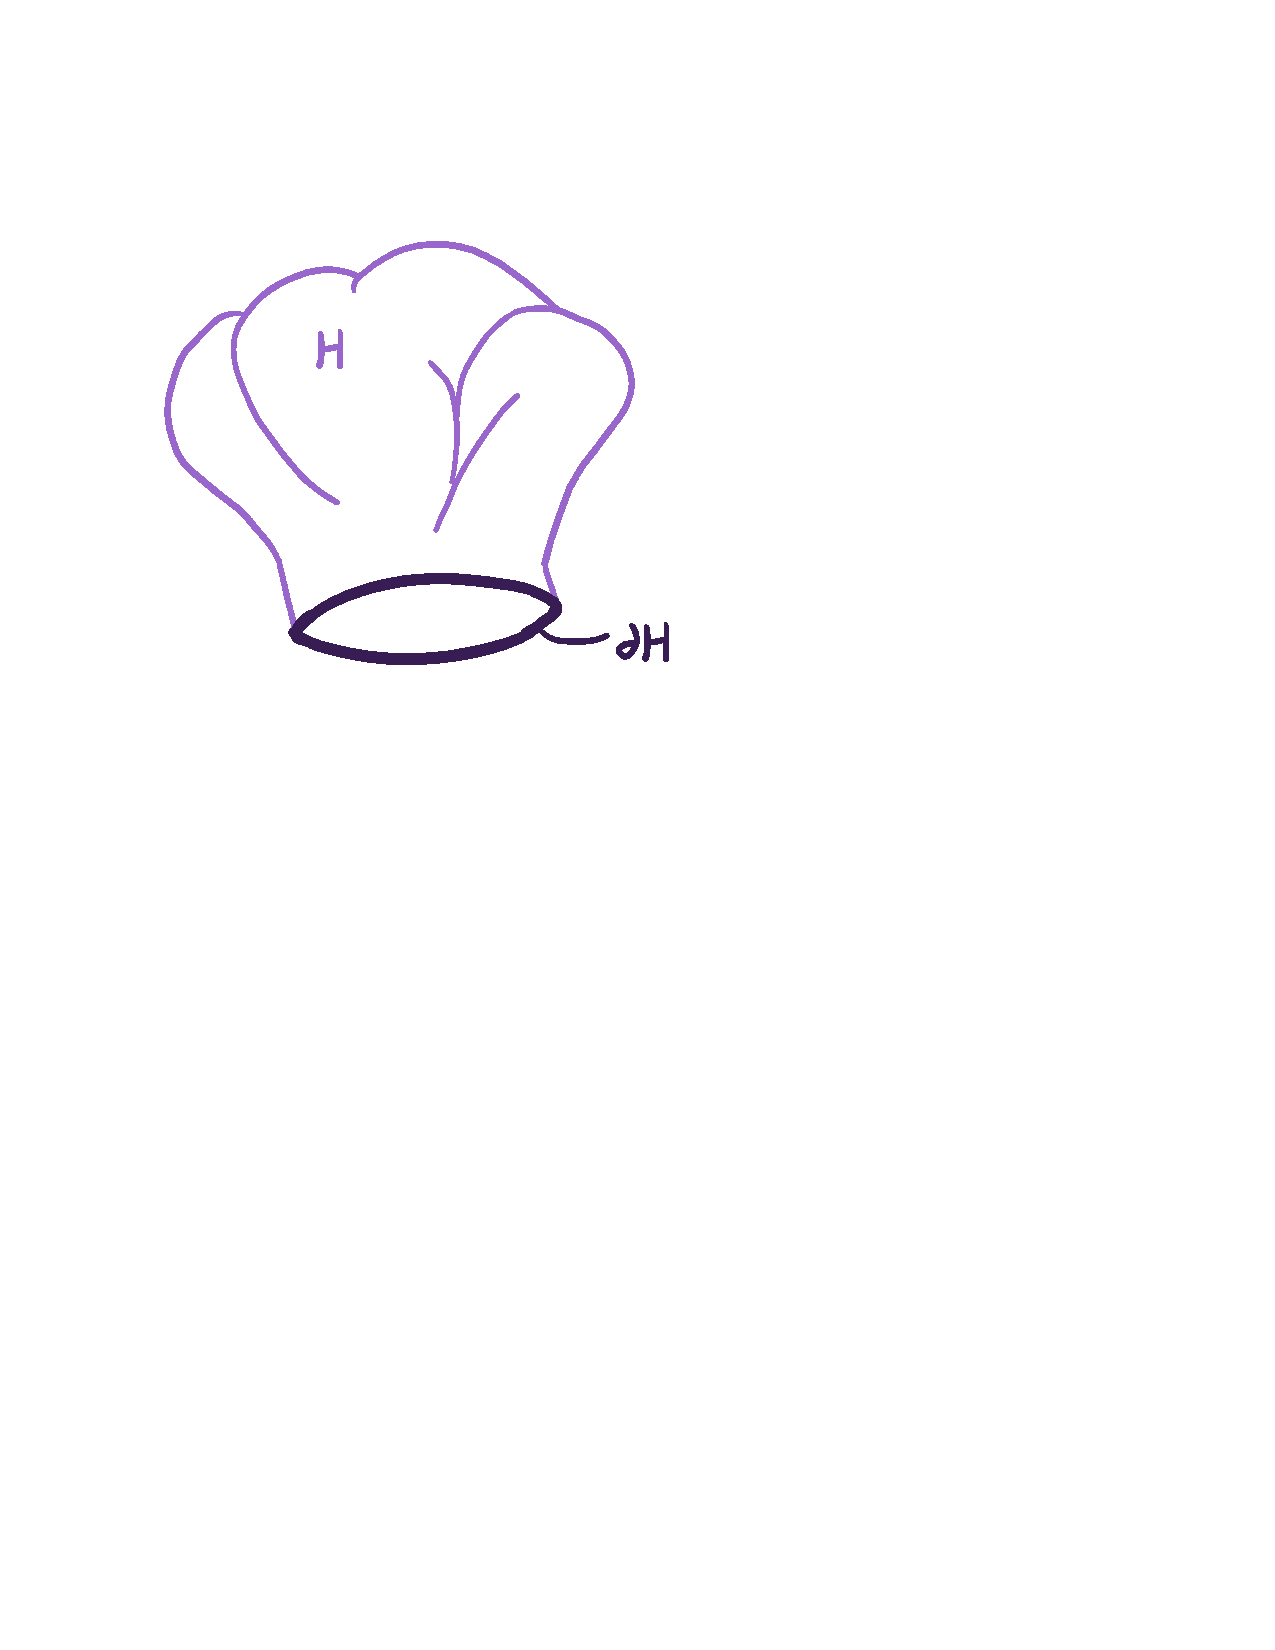
\includegraphics[scale=0.65]{chef-hat.pdf}\\
\end{center}
Then we can write:
\begin{align*}
\int_H dx\wedge dy = \pi \qquad\qquad \int_H dy \wedge dz = \int_H dx\wedge dz = 0
\end{align*} 

\hfill\break\hfill\break\hfill\break
\example Consider the sphere $S^2= \{(x,y,z)\mid x^2+y^2+z^2 = 1\}$.\\ Intuitively one can write:
\begin{align*}
\int_{S^2} dx\wedge dy  = \int_{S^2} dy\wedge dz = \int_{S^2} dx\wedge dz = 0
\end{align*}
\begin{align*}
\int_{S^2} x\, dx\wedge dy = \int_{S^2} y \, dx\wedge dy = 0
\end{align*}
Let $S^2_+$ denote the upper hemisphere, we can write:
\begin{align*}
\int_{S^2} z \, dx\wedge dy = 2\int_{S^2_+} \sqrt{1-x^2-y^2} \, dx\wedge dy = 4\pi \int_0^1 \sqrt{1-r^2}\, r \, dr = \frac{4\pi}{3}
\end{align*}

\hfill\break\hfill\break\hfill\break

Now we will prove the generalized Stokes' Theorem, which is a general theorem about integrals of differential forms that includes the three basic theorems of vector integral calculus, the Green's theorem, the Stokes' theorem, and the divergence theorem, as special cases.\\

We will begin with a lemma that is in some sense a special case of the Stokes' Theorem:

\begin{lem}
Let $I = [0,1]$, and let $I^k$ denote the unit $k$-cube in $\R^k$:
\begin{align*}
I^k = [0,1]^k = [0,1]\times [0,1]\times \cdots [0,1]
\end{align*}
Let $k>1$, let $\eta$ be a $k-1$ form defined on an open subset $U$ of $\R^k$ containing $I^k$. If $\eta$ vanishes at all points of $\Bd(I^k)$ except possibly at points of the subset $(\Int(I^{k-1}))\times \{0\}$, then we have:
\begin{align*}
\int_{\Int(I^k)}\, d\eta = (-1)^{k} \int_{\Int(I^{k-1})} b^*\eta \tag{*}
\end{align*}
with the function $b:I^{k-1} \to I^k \ \ \ \ (u_1,u_2,\cdots, u_{k-1}) \mapsto (u_1,u_2\cdots, u_{k-1},0)$. 
\end{lem}
\begin{proof}
First we note that $\Int(I^k)$ is the open cube $(0,1)^k$, and $\Bd(I^k) = I^k \setminus \Int(I^k)$. Given $j \in \N$ with $1\leq j \leq k$, let $I_j$ be the $(k-1)$-tuple $I_j=(1,2,\cdots, j-1, j+1, \cdots, k)$. Here we can write:
\begin{align*}
dx_{I_j} \coloneqq dx_1 \wedge dx_2 \cdots \wedge dx_{j-1}\wedge dx_{j+1}\wedge \cdots \wedge dx_k
\end{align*}
Since the integrals in equation (*) are linear and the operator $d$ and pullback are linear, it suffices to consider the case where $\eta = f\, dx_{I_{j}}$ with some $0$-form $f$. First, by Fubini's Theorem we can write the following:
\begin{align*}
\int_{\Int(I^k)} d\eta 
&= \int_{\Int(I^k)} df \wedge dx_{I_j} \\
&= \int_{\Int(I^k)} \left( \sum_{i=1}^k D_i fdx_i\right) \wedge dx_{I_j}\\
&= \int_{\Int(I^k)} (-1)^{j-1}(D_j f)\, dx_1 \wedge dx_2 \wedge \cdots \wedge dx_k\\
&= (-1)^{j-1}\int_{\Int(I^k)} D_j f\\
&= (-1)^{j-1}\int_{I^k} D_j f\\
&= (-1)^{j-1}\int_{\vec{v}\in I^{k-1}}\int_{x_j \in I} D_j f(x_1, x_2,\cdots, x_k)
\end{align*}
where $\vec{v} = (x_1,x_2,\cdots, x_{j-1}, x_{j+1}, \cdots, x_k)$. By the Fundamental Theorem of Calculus, we have the following:
\begin{align*}
\int_{x_j \in I} D_j f(&x_1, x_2,\cdots, x_k)\\ 
&= f(x_1,x_2,\cdots, x_{j-1}, 1, x_{j+1}, \cdots, x_k) - f(x_1,x_2,\cdots, x_{j-1}, 0, x_{j+1}, \cdots, x_k)
\end{align*}
By assumption, $\eta$, and hence $f$, vanish at all points of $\Bd(I^k)$ except possibly at points of the subset $(\Int(I^{k-1}))\times \{0\}$. Then we can write:
\begin{align*}
\int_{x_j \in I} D_j f(x_1, x_2,\cdots, x_k)  = \begin{cases}
0 & j \neq k\\
-f(x_1,x_2,\cdots, x_{k-1}, 0) & j=k
\end{cases}
\end{align*}
Concluding the results we get:
\begin{align*}
\int_{\Int(I^k)} d\eta  = 
\begin{cases} 0  & j\neq k\\
(-1)^k \int_{I^{k-1}}(f\circ b) & j=k
\end{cases}
\end{align*}
On the other hand, let $I_{k-1}$ denote the $(k-1)\times (k-1)$ identity matrix, we can write:
\begin{align*}
Db(\vec{u}) =\bmat{1&0&0 & \cdots & 0& 0\\
0&1&0 & \cdots & 0& 0\\
0&0&1 & \cdots & 0& 0\\
\vdots&\vdots&\vdots & & \vdots& \vdots\\
0&0&0 & \cdots & 1& 0\\
0&0&0 & \cdots & 0& 1\\
0&0&0 & \cdots & 0& 0}= \bmat{I_{k-1} \\ \vec{0}} \qquad\qquad \forall \vec{u}\in \R^{k-1}
\end{align*}
Then by Theorem 32.2 on Munkres, we can write:
\begin{align*}
b^*(dx_{I_j}) = \det\left(\frac{\partial (b_1, b_2,\cdots, b_{j-1}, b_{j+1}, \cdots, b_k)}{\partial (x_1,x_2,\cdots, x_{k-1})}\right) dx_1 \wedge dx_2 \wedge \cdots \wedge dx_{k-1}
\end{align*}
with $\vec{u}\in \R^{k-1}$, here $\frac{\partial (b_1, b_2,\cdots, b_{j-1}, b_{j+1}, \cdots, b_k)}{\partial (x_1,x_2,\cdots, x_{k-1})} (\vec{u})$ is the matrix formed by removing the $j$-th row of the matrix $Db(\vec{u})$. Combining with the value of $Db(\vec{u})$, we can write:
\begin{align*}
b^*(dx_{I_j}) = \begin{cases}
0 & j<k \\
dx_1 \wedge dx_2 \wedge \cdots \wedge dx_{k-1} & j=k
\end{cases}
\end{align*}
Here we can conclude that:
\begin{align*}
\int_{\Int(I^{k-1})} b^*\eta = \begin{cases}
0 & j\neq k\\
\int_{\Int(I^{k-1})}(f\circ b) & j=k
\end{cases}
\end{align*}
Here we see that the results follows.
\end{proof}


\begin{thm}[The Generalized Stokes' Theorem]
Let $k>1$, let $M$ be a compact oriented $k$-manifold in $\R^n$, with $\partial M$ having the induced orientation if $\partial M$ is not empty, let $\omega$ be a $(k-1)$-form defined in an open set of $\R^n$ containing $M$, then we have the following holds if $\partial M$ is not empty:
\begin{align*}
\int_M d\omega  = \int_{\partial M}\omega
\end{align*}
and we have the following holds if $\partial M$ is empty:
\begin{align*}
\int_{\partial M}\omega = 0
\end{align*}
\end{thm}
\begin{proof}
Here we consider two cases: 
\begin{enumerate}[topsep=3pt,itemsep=-1ex,partopsep=1ex,parsep=1ex]
\item Consider a point $\vec{p}\in M \setminus \partial M$
\item Consider a point $\vec{p}\in \partial M$
\end{enumerate}
For case (1), choose a coordinate patch $\alpha:U \to V$ belonging to the orientation of $M$, such that $U$ is open in $\R^k$ containing the unit cube $I^k$ defined in Lemma 32.0.2, and such that $\alpha$ carries a point of $I^k$ to the point $\vec{p}$. Here we note that, if we begin with an arbitrary coordinate patch $\alpha': U' \to V$ about $\vec{p}$ belonging to the orientation of $M$, one can obtain our desired coordinate patch $\alpha$ by a translation and possibly a stretching in $\R^k$. Let $W = \Int(I^k)$, and let $Y = \alpha(W)$, then the map $\alpha:W \to Y$ is still a coordinate patch belonging to the orientation of $M$ about the point $\vec{p}$, with $W = \Int(I^k)$ open in $\R^k$. Since the operator $d$ and the integrals involved are linear, it suffices to consider the special case $\omega$ being a $(k-1)$-form such that the set $C\coloneqq M\cap (\supp(\omega))$ is a subset of $Y$. Note that the suppose of $d\omega$ is contained in the support of $\omega$, hence the set $M\cap (\supp(\omega))$ is contained in $C$, which is contained in $Y$. Let $\eta$ denote the $(k-1)$-form $\alpha^*\omega$, we see that the definition of domain of the $(k-1)$-form $\eta$ can be extended to an open subset of $\R^k$ containing $I^k$, and we have $\eta$ vanishes outside of $\Int(I^k)$ as $\omega$ vanishes outside of $W$. Thus we now can apply Lemma 32.0.2, with $\alpha^*d\omega = d(\alpha^*\omega) = d\eta$:
\begin{align*}
\int_M d\omega = \int_{\Int(I^k)}\alpha^*d\omega = \int_{\Int(I^k)} d\eta = (-1)^k \int_{\Int(I^{k-1})} b^* \eta
\end{align*}
In this case, the form $\eta$ vanishes outside of $\Int(I^k)$, and hence $\eta$ vanishes on $I^{k-1}\times \{0\}$, so we have:
\begin{align*}
\int_M d\omega = (-1)^k \int_{\Int(I^{k-1})} b^* \eta  = (-1)^k \int_{\Int(I^{k-1})}0 = 0
\end{align*}
If $\partial M$ is empty, the result follows, and if $\partial M$ is nonempty, we note that the support of $\omega$ is disjoint from $\partial M$, hence $\int_{\partial M}\omega = \int_M \partial \omega$ as desired.\\

Now consider the second case where $\vec{p}\in \partial M$. Here we choose a coordinate patch $\alpha:U \to V$ belonging to the orientation of $M$, such that $U$ is a subset of $\mathbb{H}^k$ being open in $\mathbb{H}^k$, $U$ contains $I^k$, and such that $\alpha$ carries a point of $\Int(I^{k-1}) \times \{0\}$ to the point $\vec{p}$. Here we let $W = (\Int(I^k))\cup (\Int(I^{k-1}) \times \{0\})$, and let $Y = \alpha(W)$, then the map $\alpha:W \to Y$ is still a coordinate patch belonging to the orientation of $M$ about the point $\vec{p}$, with $W$ being open in $\mathbb{H}^k$ but not open in $\R^k$. Since the operator $d$ and the integrals involved are linear, it suffices to consider the special case $\omega$ being a $(k-1)$-form such that the set $C\coloneqq M\cap (\supp(\omega))$ is a subset of $Y$. Note that the suppose of $d\omega$ is contained in the support of $\omega$, hence the set $M\cap (\supp(\omega))$ is contained in $C$, which is contained in $Y$. Let $\eta$ denote the $(k-1)$-form $\alpha^*\omega$, we see that the definition of domain of the $(k-1)$-form $\eta$ can be extended to an open subset of $\R^k$ containing $I^k$, and we have $\eta$ vanishes at all points of $\Bd(I^k)$ except possibly at points in $\Int(I^{k-1})\times \{0\}$, as $\omega$ vanishes outside of $W$. Thus we now can apply Lemma 32.0.2. First note that $Y$ intersects $\partial M$ non-trivially, and we have $\Int(W) = \Int(I^k)$. Here we can compute:
\begin{align*}
\int_M d \omega = \int_{\Int(I^k)} d\eta = (-1)^k \int_{\Int^{k-1}} b^*\eta \tag{**}
\end{align*}
Now notice that $\partial M \cap (\supp(\omega))$ is covered by the following coordinate patch on $\partial M$:
$$\beta: \Int^{k-1}\to Y \cap \partial M \ \ \ \vec{x}\mapsto (\alpha\circ b)(\vec{x})$$ 
Note that $\beta$ belongs to the induced orientation of $\partial M$ if $k$ is even, and to the opposite orientation if $k$ is odd. If we use $\beta$ to compute the integral of $\omega$ over $\partial M$, we must reverse the sign of the integral when $k$ is odd. Thus now we can write:
\begin{align*}
\int_{\partial M} \omega = (-1)^k \int_{\Int(I^{k-1})} \beta^*\omega
\end{align*}
Since we have $\beta^*\omega = (\alpha \circ b)^* \omega = b^*\alpha^*\omega = b^*\eta$, comparing with equation (**) we see that the result of Theorem 31.1 follows.
\end{proof}


\example
Let $H$ be a chef hat in $\R^3$, which is a manifold, the boundary of $H$ is a circle, here we suppose further that the boundary of $H$ is a circle of radius $1$ that lies on the $xy$-plane.\\ 
\begin{center}
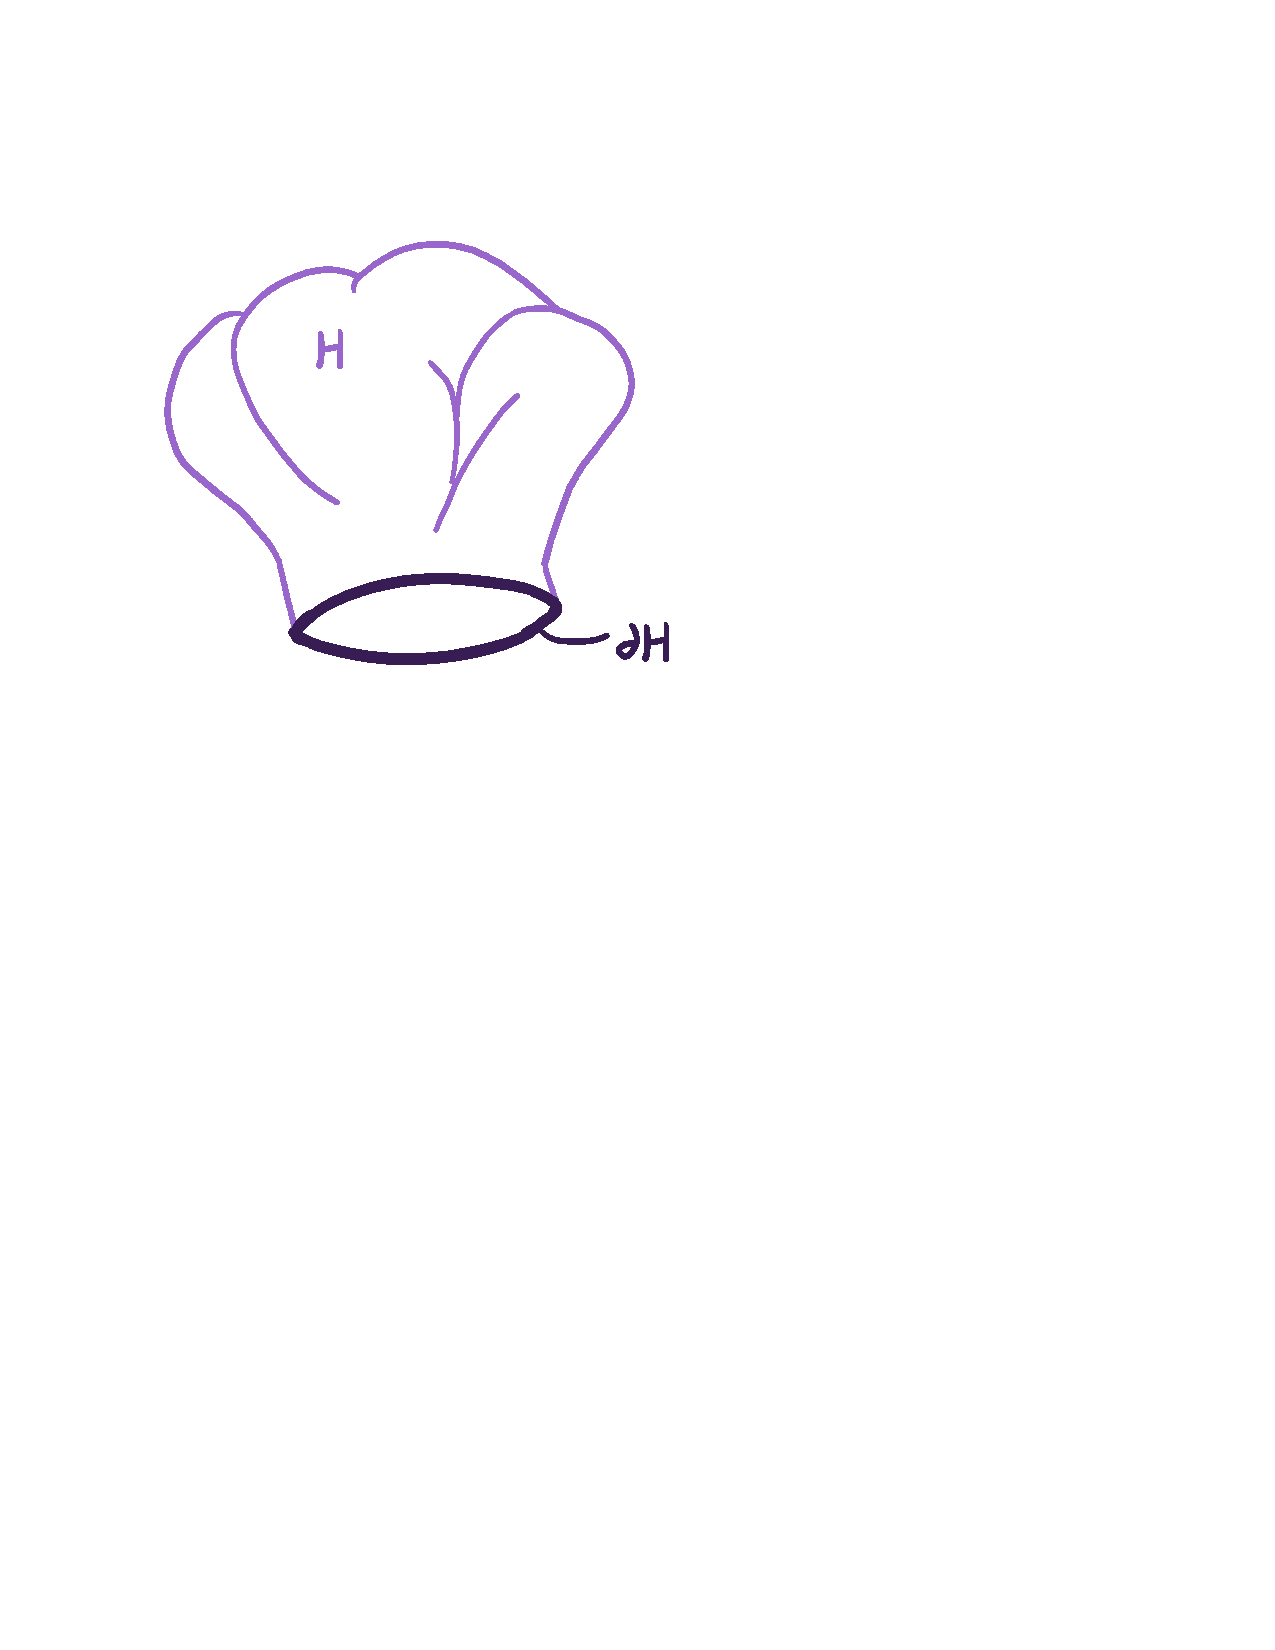
\includegraphics[scale=0.65]{chef-hat.pdf}
\end{center}
Let $M = \{ (x,y,0) \mid x^2 + y^2 \leq 1\}$, here we have $\pd M = \{ (x,y,0) \mid x^2 + y^2 = 1\} = \pd H$. We can write:
\begin{align*}
 \int_{H} dx\wedge dy = \int_{\pd H} x \, dy=\int_{\pd M} x \, dy = \int_{M}\, dx \wedge dy = \pi
\end{align*}
Here we can also write:
\begin{align*}
\int_{H} dy \wedge dz = \int_{\pd H} ( -z \, dy) = 0 \qquad\qquad\qquad \int_{H}dx \wedge dz = \int_{\pd H} (-z \wedge dy) = 0
\end{align*}
\hfill\break\hfill\break



\example 
For a sphere of radius $1$, denoted as $S^2 \in \R^3$, we can write the following:
\begin{align*}
 \int_{S_2} dx \wedge dy = \int_{\pd S_2}x \, dy = 0
\end{align*}
Similarly, we can write:
\begin{align*}
0 = \int_{S^2} dy \wedge dz = \int_{S^2} dx \wedge dz
\end{align*}
We can also write:
\begin{align*}
\int_{S^2} x\, dx \wedge dy = \int_{\pd S^2} \frac{x^2}{2}\, dy = 0
\end{align*}
Similarly we have:
\begin{align*}
 \int_{S^2} y \, dx \wedge dy = 0
\end{align*}
Now let $B^3 \coloneqq \{ (x,y,z) \in \R^3 \mid x^2 + y^2 + z^2 \leq 1\}$, we know that $\pd B^3 = S^2$. \\
Here we can write:
\begin{align*}
\int_{S^2} z \, dx \wedge dy = \int_{B^3} dz \wedge dx \wedge dy = \int_{B^3} dx \wedge dy \wedge dz = \frac{4\pi }{3}
\end{align*}
\hfill\break\hfill\break

\example Let $M = \{ (x,y,z) \mid x^2 + y^2 =1 , \ 0 \leq z \leq 1\}$. Here we define a $1$-form $\omega$:
\begin{align*}
\omega:\R^3\setminus\{(x,y,z) \in \R^3 \mid x=y=0\} \to \R^3_{row} \qquad (x,y,z)\mapsto \frac{-y\, dx + x \, dy}{x^2 + y^2}
\end{align*}
We have the following holds:
\begin{align*}
 \int_{M} d\omega = \int_{\pd M} \omega = 2\pi -2 \pi =  0
\end{align*}

\blfootnote{We have learned 100 pages of multivariable calculus, YAY!}



\newpage
\section[Application in Vector Calculus]{\color{red}Application in Vector Calculus\color{black}}

\begin{defn}
Let $A$ be an open subset of $\R^n$. \\
Any function of the form $f: A \to \R$ is called a scalar field.
\end{defn}

\begin{defn}
Let $A $ be an open subset of $\R^n$. \\
Any function of the form $v :A \to \R^n$ is called a vector field.
\end{defn}

\example \\
Velocity of fluid defines a vector field, while force field can be viewed as $1$-form.\\

\begin{defn}
Let $\alpha$ be a local diffeomorphism, let $v$ be a vector field defined on an open subset $A$ of $\R^n$. The function $\alpha^*v \coloneqq (D\alpha)^{-1} \cdot (v\circ \alpha)$ is called the pullback of vector field $v$ by $\alpha$. 
\end{defn}

For $1$-form $\omega$, we see that $\omega^T\coloneqq \left(\omega(\vec{x})\right)^T$ is a vector field, here for $\alpha$ being a local diffeomorphism such that $\omega \circ \alpha$ is well defined, we can write the following, for all $\vec{x}$ in the definition of domain of $\alpha$:
\begin{align*}
((\alpha^*\omega)(\vec{x}))^T = (\omega(\alpha(\vec{x})) \cdot D\alpha(\vec{x}))^T = (D\alpha(\vec{x}))^T \cdot (\omega(\alpha(\vec{x})))^T 
\end{align*}
Here we see that:
\begin{align*}
(\alpha^*\omega)^T = \alpha^*(\omega^T)\qquad \iff \qquad (D\alpha(\vec{x}))^T = (D\alpha(\vec{x}))^{-1}
\end{align*}
Note that $(D\alpha(\vec{x}))^T = (D\alpha(\vec{x}))^{-1}$ for all $\vec{x}$ in the definition of domain of $\alpha$ if and only if $\alpha$ is orthogonal, and by Theorem 20.5 on Munkres, this is true if and only if $\alpha$ is an isometry.\\


Exterior Calculus in $\R^3$ works well with diffeomorphism. Differential forms in $\R^3$ has the following forms, with $\alpha,\beta,\gamma$ being scalar functions, or $0$-forms defined on $\R^3$:
\begin{enumerate}[topsep=3pt,itemsep=-1ex,partopsep=1ex,parsep=1ex]
\item $0$-forms $f$
\item $1$-forms $\alpha\, dx + \beta\, dy + \gamma\, dz$
\item $2$-forms $\alpha\, dy \wedge dz + \beta \, dz\wedge dx + \gamma\, dx\wedge dy$
\item $3$-forms $f \, dx \wedge dy\wedge dz$
\end{enumerate}

Vector Calculus in $\R^3$ works well with isometry.
\begin{enumerate}[topsep=3pt,itemsep=-1ex,partopsep=1ex,parsep=1ex]
\item Scalar Fields $f$, corresponding to $0$-forms or $3$-forms defined on $\R^3$.
\item Vector Fields $v$, corresponding to $1$-forms, or $2$-forms defined on $\R^3$. 
\end{enumerate}

\note Isometries defined on $\R^2$, or $\R^3$, consist of translations, rotation, and reflection. \\

In the following table, we compare objects in exterior calculus to objects in vector calculus. One will find that, on each row, the object on the right column can be interpreted in a way very similar to the object on the left column. First we restrict our view in $\R^3$, and assume that $f:\R^3 \to \R$ is a scalar field of $C^1$ type, $\alpha,\beta,\gamma$ are $0$-forms, $\omega,\zeta,\nu$ are $1$-forms, $\mu$ is $2$-form, all defined on $\R^3$, and $\vec{F}, \vec{F}_1,\vec{F}_2$ are vector fields defined on $\R^3$, with $\vec{F}$ defined by the following:
$$\vec{F}: \R^3 \to \R^3 \ \ \ \ \vec{x}\mapsto \bmat{\alpha(\vec{x})\\ \beta(\vec{x}) \\ \gamma(\vec{x})}$$
Here we get the table:
\begin{center}
\begin{tabular}{|c|c|}
\hline
\cellcolor{orange!29} Exterior Calculus & \cellcolor{blue!29} Vector Calculus \\
\hline
Exterior derivative operator $d$ & Del operator $\nabla = \left(\frac{\partial}{\partial x}, \ \frac{\partial }{\partial y},\ \frac{\partial}{\partial z} \right)$\\
\hline
$df$ & The gradient of $f$, $\text{grad}(f) \coloneqq \nabla f$ \\
\hline
$d(\alpha dx + \beta\, dy + \gamma\, dz)$ & The curl of $\vec{F}$, $\text{curl}(\vec{F}) \coloneqq \nabla \times \vec{F}$\\
\hline
$d\left(\alpha\, dy\wedge dz + \beta dz\wedge dx + \gamma dx\wedge dy\right)$ & The divergence of $\vec{F}$, $\text{div}(\vec{F}) \coloneqq \nabla \cdot \vec{F} = \left< \nabla , \vec{F}\right>$\\
\hline
$\omega \wedge \mu$& Scalar field $\left<\vec{F}_1, \vec{F}_2\right>$\\
\hline
$\omega \wedge \zeta$& Vector field $\vec{F}_1 \times \vec{F}_2$ \\
\hline
$\omega \wedge \zeta \wedge \nu$& Scalar field $\det\bmat{\vec{F}_1,\vec{F}_2,\vec{F}_3}$\\
\hline
\end{tabular}
\end{center}

Now in $\R^2$, we note that exterior calculus in $\R^2$ works well with diffeomorphism, and vector calculus in $\R^2$ works well with isometry. Here we let $f$ be a scalar field of $C^1$ type, $\alpha,\beta$ be $0$-forms defined on $\R^2$, $\omega = \alpha\, dx + \beta\, dy$ defined on $\R^2$, vector field $\vec{F}:\R^2 \to \R^2 \ \ \ \vec{x}\mapsto (\alpha(\vec{x}), \beta(\vec{x}))$, and let $M_1$ be $1$-manifold in $\R^2$, $M_2$ be $2$-manifold in $\R^2$. Here we get the table:

\begin{center}
\begin{tabular}{|c|c|}
\hline
\cellcolor{orange!29} Exterior Calculus & \cellcolor{blue!29} Vector Calculus \\
\hline
Exterior derivative operator $d$ & Del operator $\nabla = \left(\frac{\partial}{\partial x}, \ \frac{\partial }{\partial y}\right)$\\
\hline
$0$-form $k$ define on $\R^2$ & Scalar field $k$ of $C^1$ type defined on $\R^2$ \\
\hline
$1$-forms $\omega = \alpha \, dx + \beta \, dy$ & Vector field $\vec{F}$ \\
\hline
$2$-forms $f\,dx \wedge dy$ defined on $\R^2$ & Scalar field $f$\\
\hline
$1$-form $\omega$ wedged with $1$-form $\eta$ & ${}\qquad\quad$ Scalar field $\det\left(\bmat{\vec{F}_1 \vec{F}_2}\right) \qquad\quad   {}^1$ \\
\hline
$df = \frac{\pd f}{\pd x}\, dx + \frac{\pd f}{\pd y}\, dy$ & ${}\, \qquad$ Gradient of $f$, $\text{grad}(f) \coloneqq \nabla f \qquad\, {}^2$ \\
\hline
$d(\alpha\, dx + \beta \, dy) = \lr{\frac{\pd \beta}{\pd x} - \frac{\pd \alpha }{\pd y}}\, dx\wedge dy$ & Curl of $\vec{F}$, $\text{curl}(\vec{F}) \coloneqq \lr{\frac{\pd \beta}{\pd x} - \frac{\pd \alpha}{\pd y}}$\\
\hline
$\int_{M_1} \omega$ &  \qquad$\int_{M_1} \left<\vec{F}, d\vec{l} \right> = \int_{M_1} \left< \vec{F},\, \vec{T}\right> \, dV$ \qquad${}^3$\\
\hline
$\int_{M_1}df = \Delta_{M_1} f$ &\qquad\qquad $\int_{M_1}\left< \nabla f, \vec{T}\right> = \Delta_{M_1} f$\,\qquad\qquad${}^4$\\
\hline
$\int_{M_2} f\, dx \wedge dy = \int_{M_2} f$ & $\int_{M_2} f$\\
\hline
$\int_{\pd {M_2}}\omega = \int_{M_2} d\omega$ & Circulation of $\vec{F}$ along $\pd M_2$, $\int_{M_2} \, \text{curl}(\vec{F})$\\
\hline
\end{tabular}
\end{center}

${}^1$ Here $\vec{F}_1,\vec{F}_2$ are vector fields.\\
${}^2$ $\nabla f = \lr{\frac{\pd }{\pd x}, \frac{\pd }{\pd y}}f =\lr{\frac{\pd f}{\pd x}, \frac{\pd f}{\pd y}}$.\\
${}^3$ Here we define: $$d\vec{l} \coloneqq \bmat{dx \\ dy}$$ 
${}\ \,$ Since we have $\vec{F}(\vec{x}) =(\alpha(\vec{x}),\beta(\vec{x}))$, so we have $d\vec{l} = \vec{T} \, dV$.\\
\makebox[\linewidth][s]{${}^4$ The standard interpretation here is that $f$ is called the potential energy. The force}\\ 
\makebox[\linewidth][s]{${}\ \:$ associated to potential energy $f$ is defined to be $-\nabla f$, here the negative sign for force}\\
\makebox[\linewidth][s]{${}\ \:$ simplifies the conservation of energy, and work done by such force is then defined to} 
${}\ \ $ be the following:
$$\int_{M_1} \left<-\nabla f, \vec{T} \right>\, ds = -\Delta_{M_1} f$$

\begin{defn}
Let $M$ be a compact $2$-manifold in $\R^2$ with nonempty boundary, let $\vec{F}$ be a vector field defined on an open subset of $\R^2$ containing $M$. Integrating the curl of $\vec{F}$ over $M$ is called the circulation of $\vec{F}$ along $\pd M$. That is, we can write:
\begin{align*}
\text{Circulation of }\vec{F}\text{ along }\pd M \ \coloneqq \ \int_M \, \text{curl}(\vec{F})
\end{align*}
\end{defn}

Consider a vector field $\vec{F}:A \to \R^2$  measuring the velocity of a fluid, with $A$ being an open subset of $\R^2$. Let $D$ denote a disc in $\R^2$, with a circular boundary $X$ of radius $r$. Here $D$ can be viewed as a $2$-manifold in $\R^2$ with natural orientation. Here we give the $1$-manifold $X=\partial D$ the induced orientation, and denote its unit tangent field corresponding to such orientation as $\vec{T}$. The inner product defined by the following along the boundary of $D$ is called the tangential velocity of the fluid at the point $\vec{x}\in X$: 
$$\left<\vec{F}(\vec{x}), \vec{T}(\vec{x})\right>$$  
With results from above, the following integral gives the circulation of $\vec{F}$ on $X$:
$$\text{Circulation} \coloneqq \int_X \left< \vec{F}, \vec{T}\right>\, dV$$
The average tangential velocity on $X$ is defined to be the following:
\begin{align*}
\text{Average Tangential Velocity} \coloneqq \frac{\int_X \left< \vec{F},\vec{T}\right> \, dV}{\int_X \, dV} 
\end{align*}
note that the average tangential velocity has unit $[\text{Distance}]\,/\,[\text{Times}]$. \\Notice that in our settings, we have:
\begin{align*}
\int_X \, dV = 2\pi r
\end{align*}
The average angular velocity is defined to be the following:
$$\text{Average Angular Velocity} \coloneqq \frac{\int_X \left< \vec{F}, \vec{T}\right>\, dV}{ 2\pi r^2}$$
We denote:
\begin{align*}
\vec{F}:\R^2 \to \R^2 \ \ \ \ \vec{x}\mapsto \bmat{\alpha(\vec{x})\\ \beta(\vec{x})}\qquad\qquad\qquad \omega:\R^2\to \R^2_{row} \ \ \ \ \vec{x}\mapsto \alpha(\vec{x})\, dx +\beta(\vec{x}) \, dy
\end{align*}
with $\alpha,\beta$ being scalar-valued differentiable functions defined on $\R^2$. \\
Now by Stokes' Theorem, we can write the following:
\begin{align*}
\frac{\int_X \left< \vec{F}, \vec{T}\right>}{ 2\pi r^2} = \frac{\int_X \alpha\, dx + \beta\, dy}{2\pi r^2} = \frac{\int_D \left(\frac{\pd \beta}{\pd x}- \frac{\pd \alpha}{\pd y}\right)\, dx\wedge dy}{2\pi r^2} = \frac{\int_{D} \left(\frac{\pd \beta}{\pd x}- \frac{\pd \alpha}{\pd y}\right)}{2\pi r^2}  \tag{AA}
\end{align*}
Let $\vec{o}$ denote the center of the disc $D$, the angular velocity of the fluid at $\vec{o}$ is defined as the average angular velocity of the disc $D_r$, centered at $\vec{o}$, with radius $r$ tends to zero. In such case, $(\frac{\pd \beta}{\pd x}- \frac{\pd \alpha}{\pd y})$ is approximately constant, with equation (AA) we can write:
\begin{align*}
\text{Angular Velocity at }\vec{o} = \frac{1}{2} \left[\frac{\pd \beta}{\pd x}- \frac{\pd \alpha}{\pd y}\right]_{(x,y) = \vec{o}} = \frac{1}{2}\ \text{curl}(F)(\vec{o})
\end{align*}

In general, for a compact $2$-manifold $M$ and a vector field defined by the following:
$$\vec{F}:A \to \R^2 \ \ \ \vec{x} \to \bmat{\alpha(\vec{x})\\\beta(\vec{x})}$$ 
with $A$ being open subset of $\R^2$, $\alpha$, $\beta$ being scalar-valued differentiable functions defined on $A$. We can write the following by Stokes' Theorem:
\begin{align*}
\text{Circulation of }\vec{F}\text{ along }\partial M = \int_M \text{curl}( \vec{F}) = \int_{\partial M} \left< \vec{F},\vec{T}\right> \, dV = \int_{\partial M} \alpha\, dx + \beta\, dy
\end{align*}
This result is concluded as the Green's Theorem for vector calculus.\\

Let $M$ be a compact oriented $2$-manifold in $\R^3$, by Theorem 38.9 on Munkres, the circulation of a vector field $\vec{F}$ defined on $\R^3 $ along $\partial M$ is given by the following:
\begin{align*}
\int_{\partial M}\left< \vec{F}, \vec{T}\right> \, dV = \int_{M}\left< \text{curl}(\vec{F}), \vec{N}\right>\, dV
\end{align*}

%&= \int_{M} (d\omega)(\vec{p})(\vec{v}_1(\vec{p}), \vec{v}_2(\vec{p})) \, dV \\
%&= \int_{M} \left<\text{curl}(\vec{F}), (\vec{v}_1(\vec{p}))\times (\vec{v}_2(\vec{p}))\right> dV \\

where $\vec{N}$ is the unit normal field corresponding to the orientation of $M$, and $\vec{T}$ is the unit tangent vector field corresponding to the induced orientation of $\partial M$. This result is concluded as the classical version of the Stokes' Theorem. \\


Now let $\vec{p} \in \R^3$ and $r \in \R$ with $r>0$, let $\vec{v_1},\vec{v}_2$ be orthonormal vectors, let $M_r \subseteq \R^3$ be the $1$-manifold parametrized by the following function:
$$\alpha:[\,0, 2\pi)\qquad \theta \mapsto \vec{p} + r\cos(\theta) \vec{v}_1 + r\sin(\theta) \vec{v}_2$$ 
Consider a vector field $\vec{F}$ defined by the following, with $\alpha,\beta, \gamma$ being scalar valued differentiable functions defined on an open subset $A$ containing $M_r$:
$$\vec{F}:A \to \R^3 \ \ \ \vec{x}\mapsto \bmat{\alpha(\vec{x})\\ \beta(\vec{x}) \\ \gamma(\vec{x})}$$
Here $\vec{F}$ is equivalent to an $1$-form defined by $\omega = \alpha\, dx + \beta\, dy + \gamma \, dz$ defined on $A$. \\
The average angular velocity along $M_r$ is then given by the following:
\begin{align*}
\text{Average angular velocity along }M_r = \left(\text{Circulation of }\vec{F}\text{ along }M_r\right)/(2\pi r^2) = \frac{\int_{M_r} \omega}{2\pi r^2} 
\end{align*}
And the angular velocity of $\vec{F}$ at the point $\vec{p}$ is given by:
\begin{align*}
\text{Angular velocity at }\vec{p} =  \frac{1}{2}\left< \text{curl}(\vec{F})(\vec{p}), \ \vec{v}_1\times \vec{v}_2 \right> = \frac{1}{2}\det\left( \bmat{ \text{curl}(\vec{F})(\vec{p})& \vec{v}_1&  \vec{v}_2 }\right)
\end{align*}

The discussion above can be concluded more precisely following the notation from Munkres, given in the following:\\

Let $(\vec{e}_i\mid 1\leq i\leq n)$ denote the standard basis in $\R^n$, let $A$ be an open subset in $\R^n$. First we note that, each vector field $\vec{F}:A \to \R^n \ \ \ \vec{x}\mapsto \sum_{i=1}^n F_i (\vec{x}) \vec{e}_i$, with $F_i$ being component functions of $\vec{F}$, can be equivalently written as the following:
\begin{align*}
\vec{F}:A \to \R^n \times \R^n \qquad\vec{x}\mapsto \left(\vec{x};\, \sum_{i=1}^n F_i (\vec{x}) \vec{e}_i\right)
\end{align*}
and such vector field corresponds to a $1$-form defined on $A$ defined by the following:
\begin{align*}
\omega :A \to \R^n_{row}\qquad \vec{x}\mapsto \sum_{i=1}^n F_i(\vec{x}) \, dx_i
\end{align*}
In such case, we say the $1$-form $\omega$ corresponds to the vector field $\vec{F}$. 

\begin{lem}[Lemma 38.1 on Munkres]
Let $M$ be a compact oriented $1$-manifold in $\R^n$, and let $\vec{T}$ be the unit tangent vector to $M$ corresponding to the given orientation of $M$. Let $\vec{F}$ be a vector field defined in $\R^n$ and let $\omega$ be the $1$-form corresponds to $\vec{F}$. Then we have:
\begin{align*}
\int_M \omega = \int_M \left< \vec{F}, \vec{T}\right> \, dV \tag{sv}
\end{align*} 
\end{lem}
\begin{proof}
Here it suffices to consider the case where $M\cap \supp(\omega)$ is contained in the image of a single coordinate patch $\alpha:U \to V$ on $M$ belonging to the orientation of $M$. Let $F_i$ denote the component functions of $\vec{F}$. Since $\mathcal{V}(D\alpha) = \sqrt{\det((D\alpha)^T D\alpha)} = ||D\alpha||$, we can write the following:
\begin{align*}
\int_M \omega = \int_U \alpha^*\omega &= \int_U \left< \vec{F} \circ \alpha, \ D\alpha\right> \\
&= \int_U \left< \vec{F}\circ \alpha,\ \frac{D\alpha}{||D\alpha||} \right> \,\mathcal{V}(D\alpha)\\
&= \int_U \left< \vec{F}\circ \alpha,\ \vec{T}\circ \alpha \right> \,\mathcal{V}(D\alpha)\\
&= \int_M \left< \vec{F}, \vec{T}\right>
\end{align*}
The result follows.
\end{proof}

\remark The notation $dV$ in equation (sv) is sometimes denoted as $ds$ for $1$-volume. \\

\begin{thm}[The Gradient Theorem]
Let $M$ be a compact oriented $1$-manifold in $\R^n$, let $\vec{T}$ be the unit tangent vector field to $M$ corresponding to the orientation of $M$, and let $f$ be a $0$-form defined on an open subset of $\R^n$ containing $M$. If $\partial M$ is empty, then we have:
\begin{align*}
 \int_M \left< \nabla f,\ \vec{T}\right> dV = 0
\end{align*}
If $\partial M$ is not empty, and $\partial M = (\vec{x}_1,\vec{x}_2,\cdots, \vec{x}_m)$, we let $\epsilon_i = -1$ if $\vec{T}(\vec{x}_i)$ points into $M$,  and let $\epsilon_i = 1$ if $\vec{T}(\vec{x}_i)$ points out of $M$. Then we have:
\begin{align*}
 \int_M \left< \nabla f,\ \vec{T}\right> dV =  \sum_{i=1}^M \epsilon_i f(\vec{x}_i) 
\end{align*}
\end{thm}
\begin{proof}
Note that the $1$-form $df$ correspond to the vector field $\nabla f$, then by Theorem 31.1 on Munkres and Lemma 38.1 on Munkres, the result follows.
\end{proof}

Let $\vec{F}$ be a vector field defined on an open subset $A$ of $\R^n$, by Munkres Theorem 31.1, $\vec{F}$ corresponds to an $(n-1)$-form defined by the following:
\begin{align*}
\omega = \sum_{i=1}^n (-1)^{i-1}F_i\, dx_1 \wedge dx_2 \wedge \cdots \wedge dx_{i-1}\wedge dx_{i+1}\wedge \cdots \wedge dx_n
\end{align*}
where $F_i$ are the component functions of $\vec{F}$. 

\begin{lem}[Lemma 38.5 on Munkres]
Let $M$ be a compact oriented $(n-1)$-manifold in $\R^n$, and let $\vec{N}$ be the corresponding unit normal vector field, let $\vec{F}$ be a vector field defined on an open subset $A$ of $\R^n$ containing $M$, and let $\omega$ be the $(n-1)$-form corresponds to $\vec{F}$, then we have:
\begin{align*}
\int_M \omega = \int_M \left< \vec{F},\vec{N}\right> \, dV
\end{align*}
\end{lem}
\begin{proof}
Here we note that, for the case where $n=2$, it is equivalent to write the following:
\begin{align*}
\int_M \omega = \int_M \lambda\, dV 
\end{align*}
where we have:
\begin{align*}
\lambda:M \to \R \ \ \ \ \vec{p}\mapsto \omega(\vec{p})(\vec{v}_1(\vec{p}),\vec{v}_2(\vec{p})) 
\end{align*}
where $\vec{v}_1$ and $\vec{v}_2$ are functions such that for $\vec{p}\in M$, $(\vec{v}_1(\vec{p}),\vec{v}_2(\vec{p})) $ constitutes an orthonormal frame in $\T_{\vec{p}}(M)$ belonging to the given orientation of $M$. Given the result of this lemma, we can write:
\begin{align*}
\int_M \lambda\, dV  =  \int_M \left< \vec{F},\vec{v}_1\times \vec{v}_2\right> \, dV =   \int_M \left< \vec{F},\vec{N}\right> \, dV
\end{align*}
The general proof of this Lemma is given in Lemma 38.5 on Munrkes. 
\end{proof}

In the settings of Lemma 33.1.1, given $n=3$, one might consider $\vec{F}$ as the velocity of fluid with unit density, here $\int_M \omega$ is called the flux of $\vec{F}$ across $M$, which measures the rate of flow with cancellation, for which we get positive flow in a small region when $\left<\right.\vec{F}, \vec{N}\left.\right>>0$, and negative flow in such small region when $\left<\right.\vec{F},\vec{N}\left.\right>< 0$. If the fluid has density $\rho$, then fluid crosses $M$ at a velocity given by $\rho \vec{F}$. Here $\rho$ might not necessarily be a constant and can be a scalar-valued function defined on an open subset of $\R^3$ containing $M$. In general, $\vec{F}$ and $\rho$ could also be time dependent. \\

Let $\omega$ be an $n$-form defined on an open subset $A$ of $\R^n$, we note that $\omega$ can be written as the following form:
\begin{align*}
\omega = h\, dx_1\wedge dx_2 \wedge \cdots \wedge dx_n
\end{align*}
with $h$ being a scalar-valued function defined on $A$. Here $h$ is called the scalar field associated to the $n$-form $\omega$. 

\newpage
\begin{lem}[Lemma 38.6 on Munkres]
Let $M$ be a compact $n$-manifold in $\R^n$, oriented naturally, and let $\omega = h\, dx_1 \wedge dx_2 \wedge \cdots \wedge dx_n$ be an $n$-form defined on an open set of $\R^n$ containing $M$, with $h$ being the scalar field corresponds to $\omega$, then we have:
\begin{align*}
\int_M \omega = \int_M h\, dV
\end{align*} 
\end{lem}
\begin{proof}
It suffices to consider the case where the set $M\cap \supp(\omega)$ is contained in the image of a coordinate patch $\alpha:U \to V$ on $M$ belonging to the orientation of $M$. Note that $\det(D\alpha)>0$ as $\alpha$ belongs to the natural orientation of $M$, hence we can write:
\begin{align*}
\int_M \omega = \int_U \alpha^*\omega &=\int_U (\omega \circ \alpha) \\
&= \int_{U}(h\circ \alpha) \, \det(D\alpha) \\
&=\int_{U}(h\circ \alpha) \, \sqrt{\det(D\alpha)\cdot \det((D\alpha)^T)} \\
&= \int_h (h\circ \alpha) \mathcal{V}(D\alpha) \\
&= \int_U h\, dV  
\end{align*}
\end{proof}

\begin{defn}
Let $A$ be an open subset of $\R^n$, let $f:A \to \R$ be a scalar field defined on $A$, the gradient of $f$, denoted as $\nabla f$, or $\text{grad}(f)$, is a vector field defined on $A$ defined by the following:
\begin{align*}
\nabla f: A \to \R^n \qquad \vec{x}\mapsto (D_1f(\vec{x}), D_2f(\vec{x}),\cdots , D_nf(\vec{x}))
\end{align*}
One might also denote:
\begin{align*}
\nabla f(\vec{x}) = \text{grad}(f)(\vec{x}) = (\vec{x};\, (D_1f(\vec{x}), D_2f(\vec{x}),\cdots , D_nf(\vec{x})))
\end{align*}
\end{defn}

\begin{defn}
Let $A$ be an open subset of $\R^n$, let $\vec{F}:A \to \R^n$ be a vector field defined on $A$, let $F_i$ denote the component functions of $\vec{F}$, the divergence of $\vec{F}$, denoted as $\nabla \cdot \vec{F}$ or $\text{div}(\vec{F})$, is a scalar field defined on $A$ defined by the following:
\begin{align*}
\nabla \cdot \vec{F} :A \to \R \qquad \vec{x}\mapsto \sum_{i=1}^n D_iF_i(\vec{x})
\end{align*}
\end{defn}

\begin{defn}
Let $A$ be an open subset of $\R^3$, let $\vec{F}:A \to \R^3$ be a vector field defined on $A$, let $F_i$ denote the component functions of $\vec{F}$, the curl of $\vec{F}$, denoted as $\nabla \times \vec{F}$ or $\text{div}(\vec{F})$, is a vector field defined on $A$ defined by the following:
\begin{align*}
\nabla \times \vec{F} :A \to \R^3 \quad \vec{x}\mapsto(D_2F_3(\vec{x}) - D_3F_2(\vec{x}), D_3F_1(\vec{x}) - D_1F_3(\vec{x}), D_1F_2(\vec{x}) - D_2F_1(\vec{x}))
\end{align*}
One might also denote:
\begin{align*}
(\nabla \times \vec{F})(\vec{x}) 
&= \text{curl}(\vec{F})(\vec{x}) \\
&= (\vec{x}; \ (D_2F_3(\vec{x}) - D_3F_2(\vec{x}), D_3F_1(\vec{x}) - D_1F_3(\vec{x}), D_1F_2(\vec{x}) - D_2F_1(\vec{x})))
\end{align*}
\end{defn}


\begin{thm}[The Divergence Theorem]
Let $M$ be a compact $n$-manifold in $\R^n$, let $\vec{N}$ e the unit normal vector field to $\partial M$ that points outwards from $M$, and let $\vec{F}$ be a vector field defined on an open subset of $\R^n$ containing $M$, then we have:
\begin{align*}
\int_M \text{div}(\vec{F}) \, dV = \int_{\partial M}\left< \vec{F}, \vec{N}\right> \, dV
\end{align*}
\end{thm}
\begin{proof}
Here we can orient $M$ naturally such that $\partial M$ has the induced orientation. Let $\omega$ be the $(n-1)$-form corresponds to the vector field $\vec{F}$, then we can write the following by Lemma 33.1.1:
\begin{align*}
\int_{\partial M} d\omega = \int_{\partial M} \left< \vec{F}, \vec{N}\right> \, dV
\end{align*}
By Theorem 31.1 on Munkres, we have $d\omega = \text{div}(\vec{F})\, dx_1 \wedge dx_2 \wedge \cdots \wedge dx_n$. \\
Then by Lemma 33.1.2 and Stokes' Theorem, we get the following:
\begin{align*}
\int_{\partial M} \left< \vec{F}, \vec{N}\right> \, dV =\int_{\partial M} d\omega= \int_M d\omega = \int_M \text{div}(\vec{F}) \, dV
\end{align*}
The result follows.
\end{proof}
\note \\
In the settings of $\R^3$, the Divergence Theorem is sometimes called the Gauss's Theorem.\\

\example For compact oriented $3$-manifold $U$ in $\R^3$, let $\vec{F}$ be a vector field defined on an open subset of $\R^3$ containing $U$, representing the fluid velocity around $U$, let $\rho$ be a scalar field defined on an open subset of $\R^3$ containing $U$, representing the density of the fluid around $U$. The flow out of $U$ is the flux of $\rho \vec{F}$ across $\partial U$, by the Divergence Theorem, let $\omega$ denote the $(n-1)$-form corresponds to the vector field $\rho \vec{F}$, here we can write the following:
\begin{align*}
\text{Flow out of }U = \int_{\partial U}\omega = \int_U d\omega = \int_U \text{div}(\rho \vec{F})
\end{align*}

If $\text{div}(\rho \vec{F})>0$ on $U$, the fluid is said to be expanding. \\
If $\text{div}(\rho \vec{F})<0$ on $U$, the fluid is said to be contracting.\\
For incompressible fluid, $\rho$ is constant in space and time, and $\text{div}(\rho \vec{F})  =0$ on $U$.\\
\newpage

\begin{thm}[Stokes' Theorem for $2$-manifold in $\R^3$]
Let $M$ be a compact oriented $2$-manifold in $\R^3$, let $\vec{N}$ be a unit normal field to $M$ corresponding to the orientation of $M$, and let $\vec{F}$ be a vector field of $C^\infty$ type defined on an open subset of $\R^3$ containing $M$. If $\partial M$ is empty, then we have:
\begin{align*}
\int_M \left< \text{curl}(\vec{F}),\vec{N}\right> \, dV = 0
\end{align*}
If $\partial M$ is nonempty, let $\vec{T}$ be the unit tangent vector field to $\partial M$ chosen such that $\vec{N}(\vec{p}) \times \vec{T}(\vec{p})$ points into $M$ from $\vec{p}\in \partial M$, then we have:
\begin{align*}
\int_M \left< \text{curl}(\vec{F}),\vec{N}\right> \, dV = \int_{\partial M}\left< \vec{F},\vec{N}\right>\, dV
\end{align*}
\end{thm}
\begin{proof}
Let $\omega$ be the $1$-form corresponds to the vector field $\vec{F}$. Then by Theorem 31.2, the vector field $\text{curl}(\vec{F})$ corresponds to the $2$-form $d\omega$. By Lemma 33.1.1, one can write the following:
\begin{align*}
\int_M d\omega = \int_M \left< \text{curl}(\vec{F}),\vec{N}\right>\, dV
\end{align*}
If $\partial M$ is nonempty, then by Stokes' Theorem and Lemma 33.0.1, we have:
\begin{align*}
\int_M \left< \text{curl}(\vec{F}),\vec{N}\right>\, dV = \int_{M}d\omega=\int_{\partial M}\omega = \int_{\partial M}\left< \vec{F},\vec{T}\right> \, dV
\end{align*}
The result follows.
\end{proof}


For $\vec{v}_1,\vec{v}_2 \in \R^3$, we get the followings:
\begin{enumerate}[topsep=3pt,itemsep=-1ex,partopsep=1ex,parsep=1ex]
\item $\vec{v}_1\times \vec{v}_2 \in (\spa\{ \vec{v}_1,\vec{v}_2\})^\perp$
\item $||\vec{v}_1\times \vec{v}_2|| = ||\vec{v}_1|| \cdot ||\vec{v}_2|| \sin(\theta), \text{where }\theta\text{ represents the angle between} \vec{v}_1\text{ and }\vec{v}_2$
\item If $\{\vec{v}_1$, $\vec{v}_2\}$ forms a orthonormal set of vectors, then $\vec{v}_1,\vec{v}_2$ induce a positively oritented orthonormal basis for $\R^3$, given by $(\vec{v}_1,\vec{v}_2, \vec{v}_1\times \vec{v}_2)$.
\end{enumerate}

\hfill\break
\begin{thm}
Let $M$ be a compact $2$-manifold in $\Complex$, let $f \in C^1(M, \Complex)$ be holomorphic on $M \setminus \partial M$. \\
We have the following holds:
\begin{align*}
\int_{\partial M}f\, dz = 0
\end{align*}
\end{thm}
\begin{proof}
Here we can write:
\begin{align*}
\int_{\partial M}f\, dz = \int_M d(f\, dz) = \int_M df\wedge dz = \int_{M}(f'(z)\, dz) \wedge dz = \int_{M} 0 =0
\end{align*}
The result follows.
\end{proof}


\newpage
\begin{prop}[Euler's Equations for Non-viscous Incompressible Fluid]
For non-viscous incompressible fluid, let $\vec{F}$ denote the fluid velocity vector field, we have:
\begin{align*} 
\text{div}(\vec{F}) = 0 \qquad\qquad\qquad\qquad
\frac{\partial }{\partial t}\left(\text{curl}(\vec{F})\right) + \text{curl}\left(\left(\text{curl}(\vec{F})\right)\times \vec{F}\right) = \vec{0}
\end{align*}
\end{prop}
\remark Here non-viscous means that there is no fluid friction.\\
\note One can include viscosity to get the Navier–Stokes equations.\footnote{Get a million dollars by solving this or finding a counterexample!} \\

If we have $\text{curl}(\vec{F}) = \vec{0}$, then the fluid is said to be irrotational, such imcompressible irrotational fluid satisfies the Euler's Equations for Non-viscous Incompressible Fluid.\\

Consider the special case where we have: 
$$\vec{F}(x,y,z) = \bmat{\alpha(x,y)\\ \beta(x,y) \\ 0}$$ 
for some differentiable scalar-valued functions $\alpha,\beta$ defined on $\R^2$. \\If $\vec{F}$ satisfies $\text{div}(\vec{F}) = \vec{0}$, then we get the following:
\begin{align*}
\frac{\partial \alpha}{\partial x} + \frac{\partial \beta}{\partial y} = 0 \qquad\qquad\qquad
\frac{\partial \beta}{\partial x} - \frac{\partial \alpha}{\partial y} = 0
\end{align*} 
which is equivalent to say that the function $\alpha - i\beta$ is holomorphic. \\


%Let $f$ be a holomorphic function defined on an open subset $U$ of $\Complex$, and let $U$ be contained in $\bar{A}$, Cauchy Integral Theorem stated that $\int_{C_1}f(z) \, dz = \int_{C_2}f(z) \, dz$. \\




%Q4. $v_1,v_2$ being $C^\infty $ vector field on open subset $A$ of $\R^n$ induces commuter, or the Lie Bracket, $[\vec{v}_1, \vec{v}_2]$. For a $1$-form $\omega$, we have:
%\begin{align*}
%(d\omega) (\vec{v}_1,\vec{v}_2) = L_{v_1}(\omega(v_2)) - L_{v_2}(\omega(v_1)) - \omega([\vec{v}_1,\vec{v}_2])
%\end{align*}




\newpage
\chapter{Differential Equations}
\setcounter{section}{33}
\section[The Cauchy-Lipschitz Theorem]{\color{red}The Cauchy-Lipschitz Theorem\color{black}}
\begin{lem}
Let $\Phi:\R^{n+1} \to \R^n$ be a continuous function that satisfies the Partial Lipchitz Estimate:
$$||\Phi(\vec{x}_2, y) - \Phi(\vec{x}_1,y)|| \leq M||\vec{x}_2-\vec{x}_1||$$
with some $M\in (0,\infty)$, for all $\vec{x}_1,\vec{x}_2 \in \R^n$ and $y \in \R$. Let $\vec{a}\in \R^n$. Then there exists $\tau \in (0,\infty)$ such that the function $T$ defined by the following is a contraction: $$T:C([-\tau,\tau],\R^n) \to C([-\tau,\tau],\R^n)\qquad(Tf)(t)= \vec{a}+\int_0^t\Phi(f(s),s)\, ds$$ here $C([-\tau,\tau],\R^n)$ is equipped with the norm $||f||_{sup} \coloneqq \max_{t\in [-\tau,\tau]} ||f(t)||$.
\end{lem}

\begin{proof}
Take $\tau = \frac{1}{19M}$. Consider $f,g \in C([-\tau,\tau],\R^n)$, we can write the following:
\begin{align*}
||T(f) - T(g)||_{sup} 
&= \left|\left|\left(\int_{0}^t \Phi(f(s),s)\,ds \right)-\left(\int_{0}^t \Phi(g(s),s)\,ds \right) \right|\right|_{sup} \\
&= \left|\left|\int_{0}^t \Phi(f(s),s)- \Phi(g(s),s)\,ds  \right|\right|_{sup} \\
&\leq |t-0|\cdot \left|\left|\Phi(f(s),s)- \Phi(g(s),s) \right|\right|_{sup} \\
&\leq \tau\cdot \left|\left|\Phi(f(s),s)- \Phi(g(s),s) \right|\right|_{sup} \\
&\leq \tau M ||f-g||_{sup} \\
&\leq \frac{1}{19} ||f-g||_{sup}
\end{align*}
Hence we see that $T$ is a Lipchitz map on $C([-\tau,\tau],\R^n)$ with Lipchitz constant $\frac{1}{19}< 1$. We conclude that $T$ is a contraction when $\tau = \frac{1}{19M}$. This completes the proof.
\end{proof}

Given the settings in Lemma 34.0.1, by the Contraction Mapping Theorem, we see that $T$ has a unique fixed point $f \in C([-\tau,\tau],\R^n)$. That is, we have $T(f) = f$. 
\newpage

\begin{corL}
In the settings in Lemma 34.0.1, the function $T$ has a unique fixed point $f \in C([-\tau,\tau],\R^n)$ such that $f$ solves the following initial value problem:
\begin{align*}
f'(t) = \Phi(f(t),t)\ \text{for }t\in(-\tau,\tau),\qquad f(0) = \vec{a} \tag{IVP}
\end{align*}
\end{corL}
\begin{proof}
By the Fundamental Theorem of Calculus, we can write the following: 
\begin{align*}
f'(t) = (Tf)'(t) &= \frac{d}{dt} \left(\vec{a}+\int_0^t\Phi(f(s),s)\, ds\right) \\
&=  \frac{d}{dt}\left(\vec{a}\right)+\frac{d}{dt}\left(\int_0^t\Phi(f(s),s)\, ds \right) \\
&=\vec{0}+ \Phi(f(t),t) =\Phi(f(t),t)
\end{align*}
On the other hand, we have:
$$f(0) = \vec{a}+\int_0^0\Phi(f(s),s)\, ds = \vec{a}$$
The result follows.
\end{proof}

\begin{corL}
Given the settings in Lemma 34.0.1, any function $f \in C([-\tau,\tau],\R^n)$ that solves the initial value problem given by (IVP) must be a fixed point of the function $T$.
\end{corL} 
\begin{proof}
Suppose $f\in C([-\tau,\tau],\R^n)$ solves the initial problem (IVP). Then we know that $f'(t) = \Phi(f(t),t)$. Note here $\Phi$ is a continuous function and $f$ is also a continuous function, we know that composition of continuous functions is continuous, hence $f'$ is continuous. Then we know that $f'$ is integrable. Hence by the Fundamental Theorem of Calculus, we can write the following:
$$\int_0^t f' = f(t) - f(0) =f(t) - \vec{a} \qquad \Rightarrow \qquad f(t) = \vec{a}+ \int_0^t f' = \vec{a}+ \int_0^t \Phi(f(t),t) = (Tf)(t)$$
Hence we see that $(Tf)(t) = f(t)$ for all $t \in [-\tau,\tau]$, it follows that $Tf = f$, and hence $f$ is a fixed point of $T$. This completes the proof.
\end{proof}

Now combining Lemma 34.0.1, Corollary 34.0.1.1, and Corollary 34.0.1.2 with a translation on $\R$, it is easy to obtain the following result, called the Cauchy-Lipschitz Theorem, or the Fundamental Theorem of Existence and Uniqueness for Ordinary Differential Equations, or simply the Existence and Uniqueness Theorem:
\begin{thm}[Cauchy-Lipschitz Theorem]
Let $\vec{a}\in \R^n$, let $V$ be an open neighborhood of $\vec{a}$, let $I$ be a an open neighborhood of $t_0 \in \R$, and let $\Phi:V \times I \to \R^n$ be a continuous function that satisfies the Partial Lipchitz Estimate:
$$||\Phi(\vec{x}_2, y) - \Phi(\vec{x}_1,y)|| \leq M||\vec{x}_2-\vec{x}_1||$$
with some $M \in (0,\infty)$, for all $\vec{x}_2,\vec{x}_1 \in V$ and $y \in I$. Then there exists $\tau >0$ and a function $F:B_{\tau}(\vec{a}) \times (t_0 - \tau, t_0 + \tau) \to V$ uniquely determined by the following conditions:
\begin{align*}
D_{n+1}F(\vec{z},t) = \Phi(F(\vec{z},t),t) \qquad\qquad\qquad\qquad F(\vec{z},t_0) = \vec{z}
\end{align*}
\end{thm}

\begin{defn}
For $0$-forms $f_1$ and $f_2$ defined on an open subset of $\R$, we have:
$$f_1\, df_2 - f_2\, df_1 = (f_1f_2' - f_1' f_2) \, dx$$ 
Here $(f_1f_2' - f_1' f_2)$ is called the Wronskian of $f_1$ and $f_2$, denoted as $\mathcal{W}(f_1,f_2)$.
\end{defn}

\begin{lem}
If the $0$-forms $f_1,f_2$ are linearly dependent, then $\mathcal{W}(f_1,f_2) = 0$, while $\mathcal{W}(f_1,f_2) = 0$ does not imply $f_1$ and $f_2$ are linearly dependent in general. $\mathcal{W}(f_1,f_2) = 0$ implies $f_1$ and $f_2$ are linearly dependent in the cases where: (1) $f_1,f_2$ both solve the differential equation $f'' = a\, f' + b\, f$ with scalar-valued functions $a$ and $b$ defined on $\R$, and $f_1,f_2$ have no common zeros, or (2) $f_1,f_2$ are holomorphic if they were defined on some convex subset of $\Complex$. 
\end{lem}
\begin{proof}
Assume that $A$ is the connected domain of definition for $f_1$ and $f_2$, and we assume that $f_1$ is non zero on $B$, with $B$ being nonempty connected subset of $A$. Then we can write the following:
$$d\left(\frac{f_2}{f_1}\right)=\frac{f_1\, df_2 - f_2 \, df_1}{(f_1)^2}$$
Here we see that ${f_1 df_2 - f_2 \, df_1} = 0$ on $B$ if and only if $f_2/f_1$ is constant on $B$, if and only if $f_2 -cf_1 = 0$ on $B$ with constant $c$, if and only if $f_2 - cf_1 = 0$ on $A$, if and only if $f_2$ and $f_1$ are linearly independent. 
\end{proof}

\newpage


\section[Retractions]{\color{red}Retractions\color{black}}
\begin{defn}
Let $A$ be a set, let $B$ be a subset of $A$. A retraction from $A$ to $B$ is a function $R:A \to B$ that satisfies $R(x) = x$ for all $x \in B$. 
\end{defn}

\example The function defined by the following is a retraction from $\mathbb{H}^k$ to $\partial \mathbb{H}^k$: 
$$R:\mathbb{H}^k \to \partial \mathbb{H}^k \ \ \ (x_1,x_2,\cdots, x_{k-1}, x_k) \mapsto (x_1,x_2,\cdots, x_{k-1}, 0)$$

\begin{lem}
Let $M$ be a nonempty compact orientable $k$-manifold in $\R^n$ with $\partial M\neq \emptyset$. \\There exists an $(k-1)$-form of $C^\infty$ type defined on $\R^n$ such that $\int_{\partial M}\omega \neq 0$. 
\end{lem}
\begin{proof}
The lemma should follow from Math 396 HW6 Q1. \\
Lemma Y.1 on Math 396 Supplement martial also gives a proof.
\end{proof}

\begin{lem}
Let $M$ be a $k$-manifold in $\R^n$ with nonempty manifold boundary $\partial M$, and let $\omega$ be an $(k-1)$-form defined on an open subset of $\R^n$ containing $M$. If $R:M \to \partial M$ is a $C^1$ retraction, then $\partial M$ is integral for the $(k-1)$-form $\omega - R^*\omega$. 
\end{lem}
\begin{proof}
Let $\alpha:U \to V$ be a coordinate patch on $\partial M$, then we can write:
\begin{align*}
\alpha^*(\omega - R^*\omega) &= \alpha^*\omega  - \alpha^*R^*\omega= \alpha^*\omega - (R\circ \alpha)^*\omega= \alpha^*\omega - \alpha^*\omega=0
\end{align*} 
The result follows.
\end{proof}

\begin{lem}
Let $M$ be a $k$-manifold in $\R^n$ with nonempty manifold boundary $\partial M$. Let $R:M \to \partial M$ be a function of $C^1$ type and let $\eta$ be a $k$-form defined on an open subset of $\R^n$ containing $\partial M$, then $M$ is an integral for $R^*\eta$. 
\end{lem}
\begin{proof}
Here we want to show $\alpha^*R^*\eta = 0$ for coordinate patch $\alpha$ on $M$, and let $\beta$ denote a regional coordinate patch on the codomain of $R\circ \alpha$, which is a subset of $\partial M$. 
\begin{center}
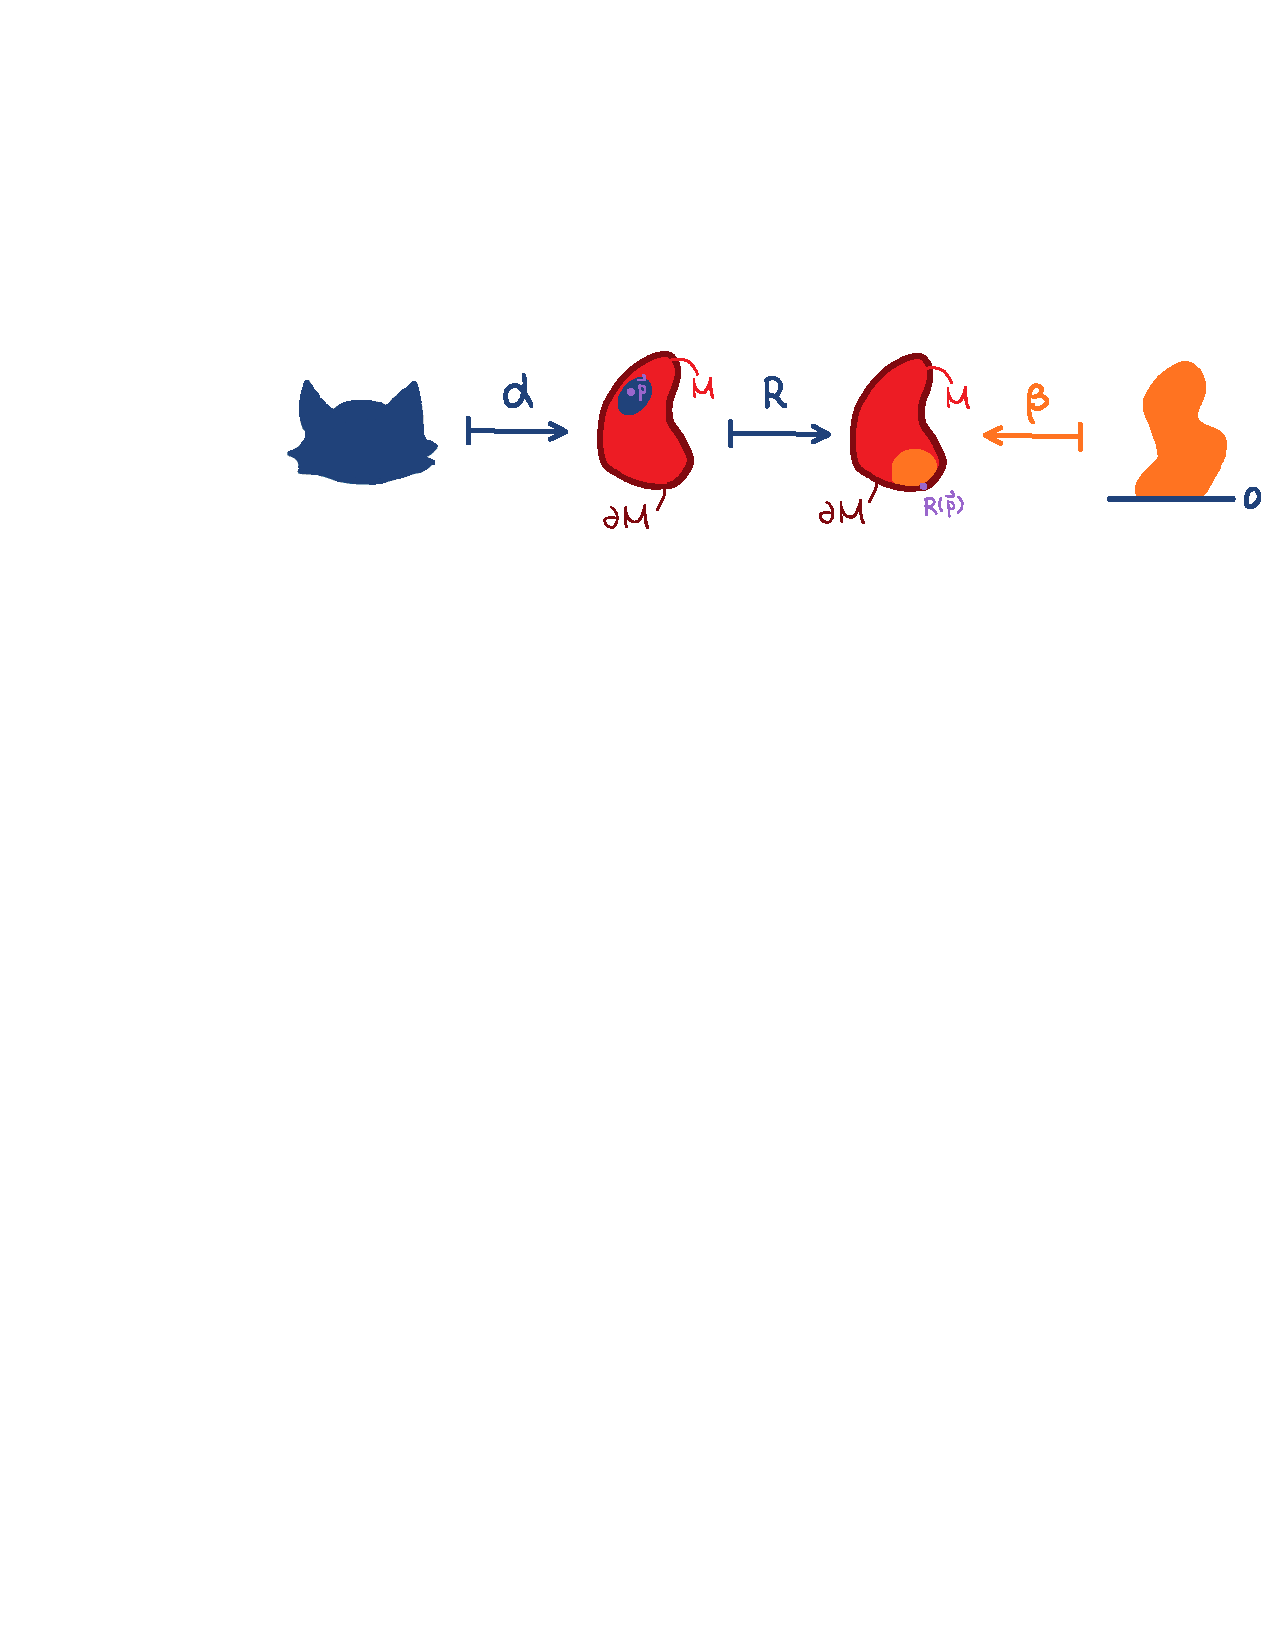
\includegraphics[scale=0.8]{retraction.pdf}
\end{center}
Here we can write:
\begin{align*}
\beta^*\eta = f\, dx_1 \wedge dx_2 \wedge \cdots \wedge dx_k
\end{align*}
for some scalar-valued function $f$, hence we can write the following:
\begin{align*}
\alpha^*R^*\eta = \alpha^*R^*(\beta^{-1})^*\beta^*\eta &= \alpha^*R^*(\beta^{-1})^*(f\, dx_1 \wedge dx_2 \wedge \cdots \wedge dx_k)\\
&= \alpha^*R^*(\beta^{-1})^*(f\, dx_1\wedge dx_2 \wedge \cdots \wedge dx_{k-1})\wedge \alpha^*R^*(\beta^{-1})^*dx_k\\
&= \alpha^*R^*(\beta^{-1})^*(f\, dx_1\wedge dx_2 \wedge \cdots \wedge dx_{k-1})\wedge d(\alpha^*R^*(\beta^{-1})^*x_k)\\
&= \alpha^*R^*(\beta^{-1})^*(f\, dx_1\wedge dx_2 \wedge \cdots \wedge dx_{k-1})\wedge d(\alpha^*R^*0)\\
&= 0
\end{align*}
Then the result follows.
\end{proof}


\begin{thm}[Non-retraction Theorem]
Let $M$ be a nonempty compact orientable $k$-manifold in $\R^n$. \\
There is no retraction of $C^1$ type from $M$ to $\partial M$. 
\end{thm}
\begin{proof}
For the case where $\partial M = \emptyset$, the result follows immediately. For the case where $\partial M \neq \emptyset$, we proceed by contradiction, suppose there exists a retraction $R:M \to \partial M$ of $C^1$ type, then by the Stokes' Theorem, Lemma 35.0.2, Lemma 35.0.3, and Lemma 35.0.4, let $\omega$ be a $(k-1)$-form defined on an open subset of $\R^n$ containing $\partial M$ such that $\int_{\partial M}\omega \neq 0$, we can write:
\begin{align*}
0 &= \int_M R^*d\omega = \int_M d(R^*\omega) = \int_{\partial M} R^*\omega = \int_{\partial M}\omega \neq 0
\end{align*}
Here we reach a contradiction, the result follows.
\end{proof}



\begin{thm}[Brouwer Fixed Point Theorem]
Let $B^n\coloneqq \{ \vec{x}\in \R^n \mid ||\vec{x}|| \leq 1 \}$ be the closed unit ball in $\R^n$. 
If $f:B^n \to B^n$ is a function of $C^1$ type, then there exists $\vec{x}\in B^n$ such that $f(\vec{x}) = \vec{x}$, and such $\vec{x}$ is called a fixed point of $f$. 
\end{thm}
\begin{proof}
Let $U = \{ \vec{x}\in B^n \mid f(\vec{x}) \neq \vec{x}\}$. Connecting $\vec{x}$ and $f(\vec{x})$ for $\vec{x}\in U$ through a line, which intersects $\partial B^n$ at two points, pick one of the two, and get $C^1$ retraction $R$ from $U$ to $\partial B^n$. 
\begin{center}
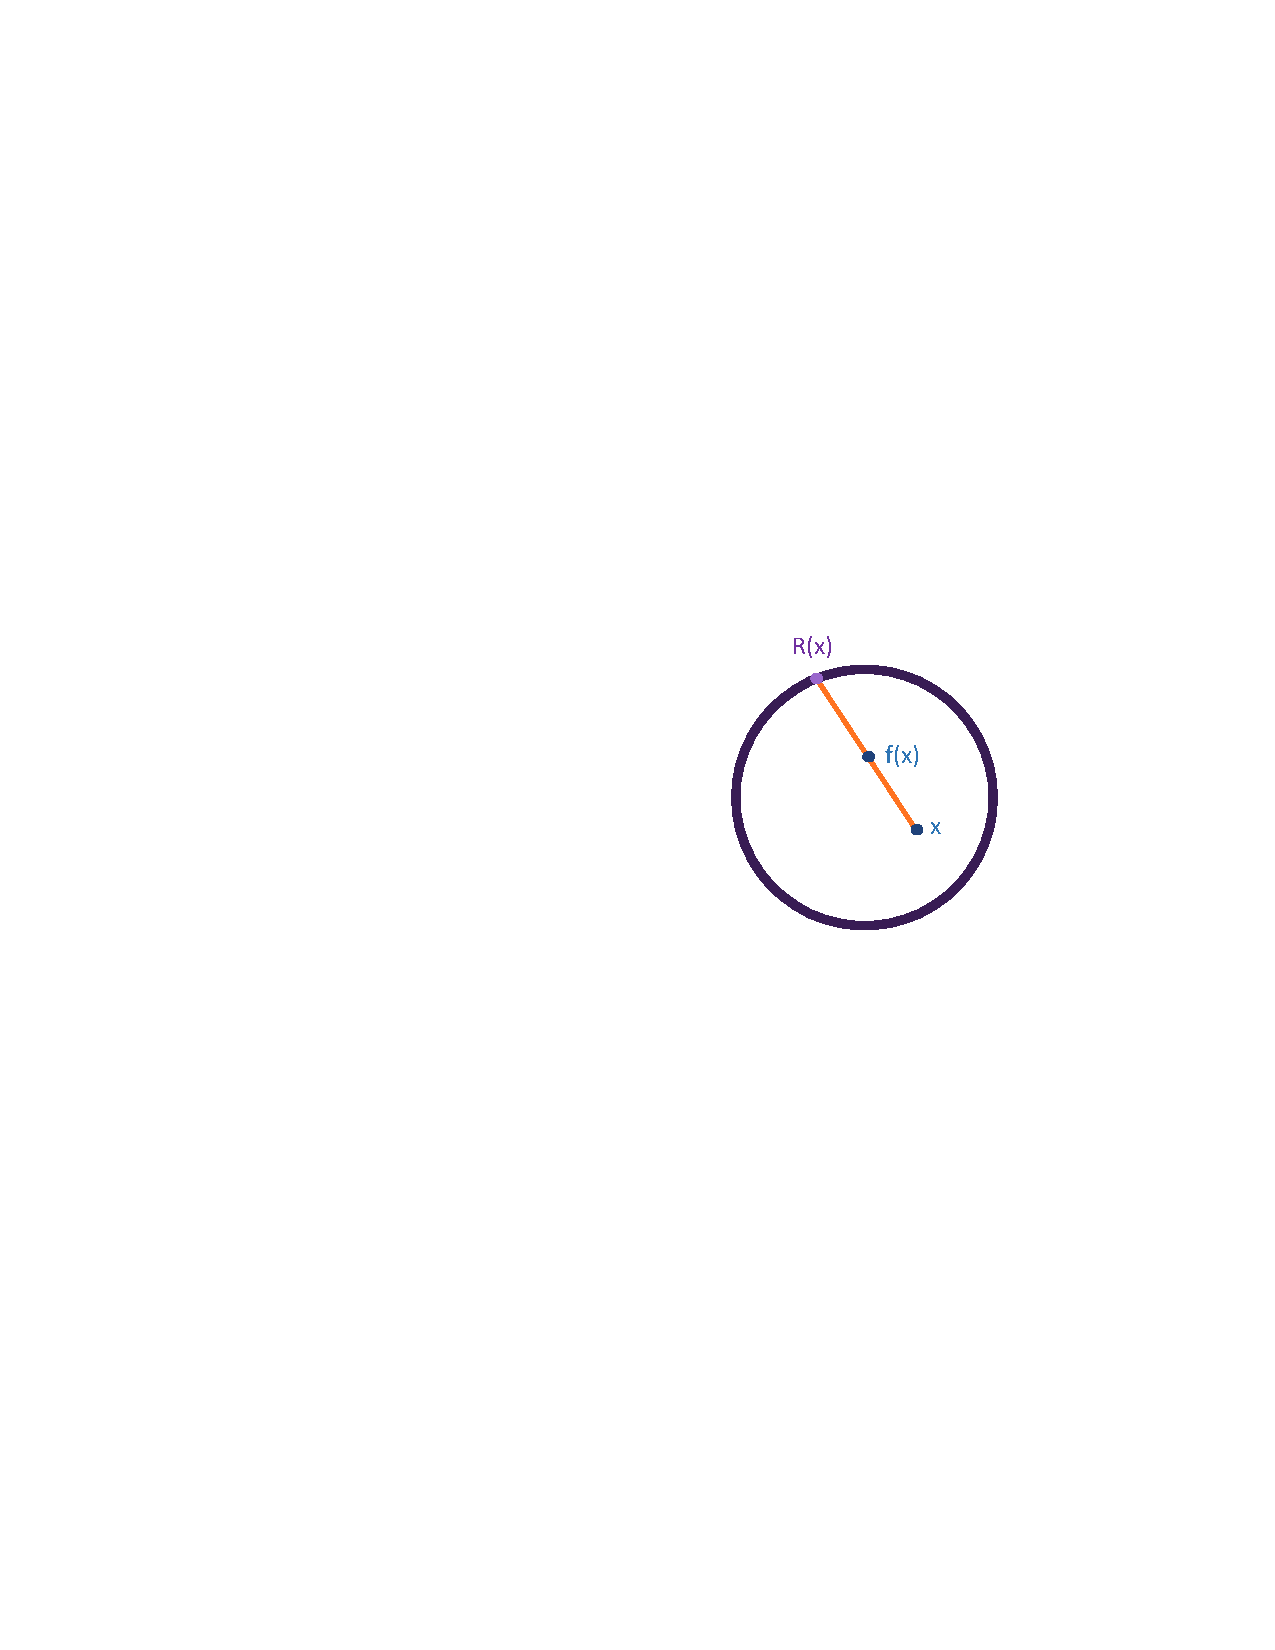
\includegraphics[scale=0.9]{fixpt.pdf}
\end{center}
Math 396 HW9 proposes a formula for such function $R$, and one can check that $R$ is a $C^1$ retraction. Non-retraction theorem implies that $U \subsetneq B^n$, and $\vec{x}\in B^n\setminus U$ is gives fixed point of $f$.
\end{proof}

\remark The result of Theorem 35.2 also holds for continuous $f$.\\
\remark For the case where $n=1$, Spivak Chapter 7 gives a proof.\\
\remark Contraction mapping theorem is also a fixed point theorem.\\

\example For discrete time dynamical system: given $f:X \to X$ defined similarly as in Theorem 35.2, one can construct a sequence $(x_1, f(x_1), f(f(x_1)), \cdots)$ with $x_1 \in X$, the fixed point of $f$ is the equilibrium. Denote $f_i = f$, define $f^{\circ\, k} \coloneqq f_1\circ f_2 \circ\cdots \circ f_k$, we get a semi-group homomorphism: 
$$H:\N \mapsto \{\text{self map of }f: X \to X\} \ \ \ k \mapsto f^{\circ \, k}$$





\newpage
\section[Equilibriums and Flows of Vector Fields]{\color{red}Equilibrium and Flow of Vector Fields\color{black}}
\begin{defn}
Let $M$ be a $k$-manifold in $\R^n$, and let $v$ be a vector field in $\R^n$. For $\vec{p} \in M$, $\vec{p}$ is called fixed point, or a equilibrium point, on $M$ associated to $v$ provided that $v(\vec{p}) = 0$. 
\end{defn}


Let $v$ be a vector field in $\R^n$ satisfying the Lipchitz estimate $||v(\vec{x}_2) - v(\vec{x}_1|| \leq M ||\vec{x}_2 - \vec{x}_1||$ for some $M>0$, and all $\vec{x}_1,\vec{x}_2 \in \R^n$. By the Existence and Uniqueness Theorem, one can solve the following ODE for $f:A \to \R^n$ uniquely, where $A$ is a subset of $\R$:
\begin{align*}
f'(t) = v(f(t)) \qquad\qquad\qquad\qquad f(t_0 ) = \vec{z} 
\end{align*}
This result is related to the $\R$-action on $\R^n$. Equilibrium points for $f$ are points where $v$ vanishes, and this result suggests Theorem 36.1, while the proof of the theorem is left for the reader:
\begin{thm}
Let $B^n$ denote the closed unit ball in $\R^n$. If $\vec{v}$ points inwards at all points $\vec{p}$ on the boundary $\partial B^n$, then there is an equilibrium point in $B^n$. 
\end{thm}
\hfill\break

Now consider a vector field $v:\R^n \to \R^n$ satisfying the Lipchitz Estimate, that is, for $\vec{x}_1,\vec{x}_2 \in \R^n$, we can write the following, with $M\in (0,\infty)$:
\begin{align*}
||v(\vec{x}_2) - v(\vec{x}_2)|| \leq M ||\vec{x}_2-\vec{x}_1|| 
\end{align*}
By Theorem 34.1, one can solve the following system with a unique function $f$:
\begin{align*}
f'(t) = v(f(t)) \qquad\qquad\qquad\qquad f(t_0) = \vec{z} \tag{*}
\end{align*}  
with $f$ defined on $(t_0 - \frac{1}{19M}, t_0 + \frac{1}{19M})$, one can check that, by manipulating the constant $19$ in the proof of Lemma 34.0.1, that $f$ is well defined on $(t_0 - \frac{1}{2M}, t_0 + \frac{1}{2M})$. \\
Now we can also solve the following system with some function $\that{f}$:
\begin{align*}
\that{f}'(t) = v(\that{f}(t)) \qquad\qquad\qquad\qquad \that{f}\left(t_0 + \frac{1}{4m}\right) = f\left(t_0 + \frac{1}{4m}\right)
\end{align*}
where $\that{f}$ is defined on $t \in (t_0 - \frac{1}{4M}, t_0+\frac{3}{4M})$. \\
By the uniqueness of $f$ and $\that{f}$, we can write:
\begin{align*}
\that{f}(t) = f(t) \qquad \forall t\in\left(t_0 - \frac{1}{4m}, t_0 + \frac{1}{2m}\right)
\end{align*}
By redefining $f$ on $(t_0 - \frac{1}{2m}, t_0+\frac{3}{4m})$, we get a solution for the initial value problem (*) on $(t_0 - \frac{1}{2m}, t_0+\frac{3}{4m})$. Continue going forward and backward on the definition of domain of $f$, one can obtain a solution for (*) on all of $\R$, and get a function $F:\R^{n+1} \to \R^n$ defined for $\vec{z}\in \R^n$, $t \in \R$, such that the following holds:
\begin{align*}
D_{n+1}F(\vec{z},t) = v(F(\vec{z},t))
\qquad\qquad\qquad\qquad
F(\vec{z},0) = \vec{z}
\end{align*}
Suppose further that $v\in C^2$, by Math 396 HW8 Q4, $F$ is of $C^1$ type. More generally, if $v\in C^{r}$, one can show that $F \in C^{r}$, and if $v \in C^\infty$, then $F \in C^\infty$. \\

Now we denote $F^s(\vec{z},t) \coloneqq F(\vec{z}, t+s)$, then one can get the following:
\begin{align*}
D_{n+1} F^s(\vec{z},t) = v(F^s(\vec{z},t)) \qquad\qquad\qquad\qquad F^s(\vec{z},0) = F(\vec{z},s)
\end{align*}
so we get $F(\vec{z},t+s) = F^s(\vec{z},t) = F(F(\vec{z},s),t)$. Then we can define:
$$g^t:\R^n \to \R^n \qquad \vec{z}\mapsto F(\vec{z},t)$$ 
with the property $g^{t+s}(\vec{z}) = g^t(g^s(\vec{z}))$ for $\vec{z}\in \R^n$, $t,s \in \R$, and $g^0$ being the identity transformation. \\

Here we denote: 
$$\text{Diffeo}(\R^n)\coloneqq \text{Diffeo}(\R^n, \R^n) \coloneqq \{\text{Diffeomorphisms from }\R^n \text{ to }\R^n\}$$ 
We define the function:
\begin{align*}
H:\R \to \text{Diffeo}(\R^n) \ \ \ \ t\mapsto g^t
\end{align*}
Here $H$ is a group homomorphism from $\R$ to $\text{Diffeo}(\R^n)$.\\

Conversely, one can show that, given a group homomorphism characterized by the following: 
$$H: \R \to \text{Diffeo}(\R^n) \ \ \ t\mapsto g^t$$ 
we get a vector field $v$ defined on $\R^n$:
$$v:\R^n \to \R^n \ \ \ \ \vec{x}\mapsto\left( D_{n+1}(g^t(\vec{x}))\right)|_{t = 0}$$

Concluding from above, let $v$ be a $C^\infty$ Partially Lipchitz vector field defined on $\R^n$, the definition of $\vec{v}$ leads to a group homomorphism $H: \R \to \text{Diffeo}(\R^n) \ \ \ t\mapsto g^t$ with $D_{n+1}(g^t(\vec{x})) = v(g^t(\vec{x}))$. Here, sometimes we denote $D_{n+1}F(\vec{z},t)$ as $D_{t}F(\vec{z},t)$. \\

A Lipchitz vector field $v:\R^n \to \R^n$ of $C^2$ type induces a unique group homomorphism from $\R$ to $\text{Diff}_{C^1}(\R^n) \coloneqq \{\text{Diffeomorphisms from }R^n \text{ to }\R^n \text{ of }C^1 \text{ type}\}$, defined by:
\begin{align*}
H : \R \to \text{Diffeo}_{C^1}(\R^n) \ \ \ t\mapsto g^t
\end{align*}
such that $D_{t}(g^t(\vec{x})|_{t=0} = v(\vec{x})$. Here $H$ is called the flow of $v$.\\

\note A function is Lipschitz and of $C^2$ type if and only if the function is of $C^2$ type with bounded first derivative.


\begin{thm}[Rectification Theorem]
Let $\vec{x}_0 \in A$ where $A $ is an open subset of $\R^n$, let $v $ be a vector field of $C^\infty$ type defined on $A$, with $v(\vec{x}_0) \neq \vec{0}$. Then there exists an open neighborhood $U$ of $\vec{x}_0$ contained in $A$, and a $C^\infty$-diffeomorphism $\alpha:U\to V$ such that $D\alpha(\vec{x})(v(\vec{x})) = \vec{e}_1$, where $\vec{e}_1 = (1,0,0,\cdots, 0)$ is the first element in the standard basis of $\R^n$. 
\end{thm}

\note Stated differently, Theorem 35.5 suggests that, given $\vec{x}_0 \in A$ where $A$ is an open subset of $\R^n$, let $v $ be a vector field of $C^{r+1}$ type defined on $A$ with $v(\vec{x}_0) \neq \vec{0}$, then there exists a $C^r$-diffeomorphism $\alpha$ such that $D\alpha(\vec{x})\cdot \vec{e}_1 = v(\alpha(\vec{x}))$. 

\begin{thm}
Let $M$ be a closed $k$-manifold without boundary in $\R^n$ of $C^\infty$ class, let $v$ be a vector field that is tangent to $M$ at all $\vec{p}\in M$, that is, we have $v(\vec{p}) \in \T_{\vec{p}}(M)$ for all $\vec{p}\in M$. Then each $g^t|_M$ induced by $v$ belongs to $\text{Diffeo}(M)$, where $\text{Diffeo}(M) \coloneqq \text{Diffeo}(M,M)$.  \footnote{Given a tangent vector field on a differentiable manifold $X$. The flow of the vector field is the group of diffeomorphisms of $X$ that lets the points of the manifold flow along the vector field, hence which sends them along flow lines, or the integral curves, that are tangent to the vector field.}
\end{thm}
\begin{proof}
It suffices to show that $g^t(M) \subseteq M$, then $(g^t)^{-1}\coloneqq g^{-t}$ also map $M$ to $M$. Let $\vec{x} \in M$, let $E \coloneqq \{ t\in \R \mid g^t(\vec{x})\subseteq M\}$, we want to show that $E = \R$. Note that we have $0 \in E$ and $E$ is closed as $M$ is closed. It suffices to show that $E$ is open. For $\vec{x}\in M$, consider two cases, case (1) $v(\vec{x}) = 0$, and case (2) $v(\vec{x})\neq 0$. For case (1), since $v(\vec{x}) = 0$, then  $g^t(\vec{x}) = \vec{x}$, and so for all $t \in \R$, $g^t(\vec{x}) \in M$. For case (2), assume that $v(\vec{x})\neq 0$, after the change of coordinate, locally, it suffices to consider the special case where we have $v(\vec{x}) = \vec{e}_1$, in which case we get $g^t(\vec{x}) = \vec{x}+ t\vec{e}_1$ for small enough $t$. Note that $M$ in such case, by Theorem 16.1, is equivalently given by $\text{Graph}(f)$, where $f \in C^1(U,\R^{n-k})$ with $U$ being convex open subset of $\R^k$. By assumption, $v(\vec{x}) = \vec{e}_1$ is tangent to $M$ at $\vec{x}$, so we must also have $D_1 f = 0$, so $f$ is independent of $q_1$ at $\vec{q}=(q_1,q_2,\cdots, q_k) \in U$ such that $\vec{x} = (\vec{q},f(\vec{q}))$. Since $U$ is convex, this implies that, if $\vec{x}+t_0 \vec{e}_1 \in M$, then $\vec{x}+t\vec{e}_1  \in M$ for $|t-t_0|<\epsilon$ for some $\epsilon>0$, then we see that $E$ is open, which completes the proof.
\end{proof}

\begin{corT}
Let $M$ be a compact $k$-manifold without boundary in $\R^n$ of $C^\infty$ class, and let $U$ be an open subset of $\R^n$ containing $M$. For vector field $v \in C^2(U, \R^n)$ such that $v$ is tangent to $M$, each $g^t|_M$ induced by $v$ belongs to $\text{Diffeo}(M)$, and there exists Lipchitz $\hat{v} \in C^2(\R^n, \R^n)$ such that $\hat{v} = v$ on some neighborhood of $M$, here the flow for $\hat{v}$ along $M$ is also a flow for $v$ along $M$.
\end{corT}
\begin{proof}
Use a partition of unity on $\R^n$, $\{\phi_j\}$ , such that $\supp(\phi_j) \cap M \neq \emptyset$ if and only if $j \leq N$, let $\hat{v} = \sum_{j=1}^N (\phi_j \, v)$. One can check that $\hat{v}$ has bounded first derivative.
\end{proof}

\example Consider $v_1:\R^2 \to \R^2 \ \ \ (x,y)\mapsto (y,-x)$.\\
Here $v$ defines a non-vanishing vector field tangent to $S^1$.\\

\example Consider $v_2:\R^4 \to \R^4 \ \ \ (x,y,a,b)\mapsto(y,-x, b, -a)$.\\
Here $v_2$ defines a non-vanishing vector field tangent to $S^3$.\\

\example Consider $v_3:\R^3 \to \R^3 \ \ \ (x_1,x_2,x_3)\mapsto(x_2,x_1,0)$.\\
Here $v_3$ defines non-vanishing vector field tangent to torus $T$.\\


\begin{thm}[Hairy Billiard Ball Theorem]
Any tangential vector field of $C^1$ type defined on an even-dimensional sphere $S^{2n}$ vanishes at some point $\vec{p}$ in $S^{2n}$. That is, "you cannot comb a hairy billiard ball without creating a cowlick."
\end{thm}
\begin{proof}
We proceed by contradiction, suppose we do have $v:S^{2n} \to \R^{2n+1}\setminus \{0\}$ with $\left<v(\vec{p}), \vec{p}\right> = 0$ for all $\vec{p}\in S^{2n}$, then we can define the following function:
\begin{align*}
h: \R^{2n+1}\setminus \{0\} \to \R^{2n+1} \ \ \ \vec{p}\mapsto\cos(||\vec{p}||-1) \frac{\vec{p}}{||\vec{p}||} + \sin(||\vec{p}||-1) \frac{v(\vec{p}/||\vec{p}||)}{||v(\vec{p}/||\vec{p}||)||}
\end{align*}
one can show that the image of $h$ belongs to $S^{2n}$. Moreover, for $||\vec{p}|| = 1$, we can write $h(\vec{p}) = \vec{p}$, and for $||\vec{p}|| = \pi +1$, we can write $h(\vec{p}) = -\vec{p}/(\pi+1)$. By Lemma 35.0.1, one can pick $(2n)$-form $\omega$ with $\int_{S^{2n}}\omega \neq 0$. By Lemma Y.2, Y.3, and Y.4 on Math 396 Supplement Materials, we see that $S^{2n}$ is an integral for $d\omega$, and $h$ defines a smooth function from $R^{2n+1}\setminus \{0\}$ to $S^{2n}$, then we have: 
$$0 = \int_{1\leq ||\vec{x}|| \leq {\pi+1}} h^*d\omega $$ 
and hence we can write the following:
\begin{align*}
0 = \int_{1\leq ||\vec{x}|| \leq {\pi+1}} h^*d\omega = \int_{1\leq ||\vec{x}|| \leq \pi+1} d(h^*\omega) = \int_{||\vec{x}|| = \pi+1}h^*\omega - \int_{||\vec{x}||=1} h^*\omega
\end{align*}
Here the diffeomorphism between $(2n)$-sphere of radius $1$ and $\pi+1$ is induced from the diffeomorphism between $(2n+1)$-ball of radius $1$ and of radius $\pi+1$:
\begin{align*}
g: \{||\vec{x}||\leq \pi+1\} \to \{ ||\vec{x}||\leq 1\} \qquad \vec{x}\mapsto - \frac{\vec{x}}{\pi+1}
\end{align*}
Note that $g$ is orientation reversing, hence we have:
\begin{align*}
0 = \int_{||\vec{x}|| = \pi+1}h^*\omega - \int_{||\vec{x}||=1} h^*\omega  =-\int_{S^{2n}}\omega - \int_{S^{2n}}\omega   \neq 0 
\end{align*}
Here we reach a contradiction. 
\end{proof}


\begin{corT}
$S^2$ is not diffeomorphic to the torus in $\R^2$. 
\end{corT}


\begin{defn}
Let $M$ be a compact naturally oriented $n$-manifold in $\R^n$, let $v$ be a vector field defined on a neighborhood of $M$, and let $\vec{N}$ denote  the unit normal field corresponds to the induced orientation of $\partial M$. $v$ is said to be inward-pointing to $M$ provided that the following holds for all $\vec{p}\in \partial M$: $$\left<v(\vec{p}), \vec{N}(\vec{p})\right> \leq 0$$
\end{defn}

\begin{defn}
Let $X$ be a subset of $\R^n$. A function $h:[0,\infty)\to C^1(X,X)$ is said to be a monoid homomorphism provided that we have $h(t) \circ h(s) = h(t+s)$ and $h(0) = Id$, where $Id$ is the identity transformation.
\end{defn}

\begin{thm}
Let $M$ be a compact $n$-manifold in $\R^n$, let $v$ be a vector field defined on an open subset of $\R^n$ containing $M$ that is of $C^2$ type and inward-pointing to $M$. The function defined by the following is a monoid homomorphism:
\begin{align*}
h: [0,\infty) \to C^1(M,M) \qquad t\mapsto g^t
\end{align*}
where we have $\left(D_t(g^t(\vec{x}))\right)|_{t=0} = v(\vec{x})$
\end{thm}

\newpage
Suppose we have an inward-pointing $v$ of $C^1$ type on $B^n$. it is easy to show that each $g^t$ induced by $v$ has at least one fixed point, a natural question arises that whether or not all $g^t$ in $\{g^t\}$ have a common fixed point, which is the point where $v$ vanishes. The answer to this question is yes, as proposed in the following theorem:

\begin{thm}
Let $v$ be a $C^1$ inward-pointing vector field on $B^n$, then $v$ must vanish some point on $B^n$.
\end{thm}
\begin{proof}
By Math 396 HW Study Exercise, there exists some $\epsilon>0$ such that the image of the function $h:B^n \to \R^n \vec{x}\mapsto \vec{x}+\epsilon v(\vec{x})$ is a subset of $B^n$. Now by Brouwer Fixed Point Theorem, there exists $\vec{x} \in B^n$ such that $h(\vec{x})  =\vec{x}$, which suggests that $v(\vec{x}) = \vec{0}$, which completes the proof.
\end{proof}

\begin{thm}[Poincare-Bendixson Theorem]
Let $v$ be a inward-pointing vector field on a compact 2-manifold $M$ in $\R^2$. Then we have either one of the two holds: (1) $v$ has a equilibrium point in $M$, or (2) there exists $t_0 > 0$ such that $g^{t_0}$ has a fixed point in $M$. 
\end{thm}


\newpage
\chapter{Complex Analysis \ \rom{2}}
\setcounter{section}{36}
\section[Residues and Contour Integrals]{\color{red}Residues and Contour Integrals\color{black}}
\begin{thm}[Cauchy Integral Theorem]
Let $M$ be a naturally oriented compact $2$-manifold in $\Complex$, let $f \in C^1(M, \Complex)$ be holomorphic on $M \setminus \partial M$, and let $\partial M$ obtain the induced orientation from $M$. then we have: 
$$\int_{\partial M}f\, dz = 0$$ 
\end{thm}
\begin{proof}
The result follows immediately from Theorem 32.1, the Stokes' Theorem.
\end{proof}

\begin{corT}
Let $M$ be a naturally oriented compact $2$-manifold in $\Complex$, let $f \in C^1 ( M,\Complex)$ be holomorphic on $M\setminus \partial M$. If $\partial M$ is the disjoint union of two $1$-manifolds $C_1$ and $C_2$, each with the induced orientation from $M$, with $C_2$ lying in the bounded component of $\Complex \setminus C_1$, then we have the following holds:
$$\int_{C_1}f \, dz = \int_{C_2} f\, dz$$
\end{corT}
\begin{proof}
This follows immediately from Theorem 37.1. Note that the orientation of $\partial M$ is obtained from the standard orientation of $M$ and the orientation of disjoint circles are opposite.
\end{proof}


\begin{thm}[Residue Theorem]
Let $M$ be a compact $2$-manifold in $\Complex$, let $E = \{z_1,z_2,\cdots, z_k\} \subseteq M\setminus \partial M$, and let $f\in C^1(M\setminus E, \Complex)$ be holomorphic on $M \setminus (\partial M\cup E)$, then we have the following holds:
$$\int_{\partial M}f\, dz = 2\pi i \sum_{j=1}^k Res(f\, dz, z_j)$$ 
\end{thm}
\begin{proof}
For each $z_j$, one can choose a circle $C_j$ centered at $z_i$ with radius small enough such that the circle is contained in $M\setminus (\partial M\cup E)$, now apply Cauchy Integral Theorem, we get the following:
\begin{align*}
0 = \int_{\partial M}f\, dz - \sum_j \int_{C_j}f\, dz
\end{align*}
The result follows.
\end{proof}

Let $\Omega$ be a connected open subset of $\Complex$, let $f,g$ be holomorphic on $\Omega$ that are not identically zero. By results from Chapter 5, $h = \frac{f}{g}$ is holomorphic on $\Omega \setminus g^{-1}(0)$, and $g^{-1}(0)$ is a discrete set, that is, it has no limit points in $\Omega$. By easy computation we get:
\begin{align*}
\frac{h'_{\Complex}}{h} = \frac{f'_{\Complex}}{f} -\frac{g'_{\Complex}}{g}
\end{align*}

\remark For holomorphic function $f$, the derivative of $f$ in complex sense, as previously denoted as $f_{\Complex}'$, might be denoted as $f'$ thereafter.\\

By Math 396 HW4 Q2, we also have the following:
\begin{align*}
Res\left(\frac{h'}{h}\, dz, z_0\right) = Res\left(\frac{f'}{f}\, dz, z_0\right) - Res\left(\frac{g'}{g}\, dz, z_0\right)= \text{ord}_{z_0}f - \text{ord}_{z_0}g
\end{align*}

Now consider a compact $2$-manifold $M\subseteq \Omega$ with $\partial M \cap (f^{-1}(0) \cup g^{-1}(0)) = \emptyset$, we have:
\begin{align*}
\frac{1}{2\pi i}\int_{\partial M}\frac{h'}{h}\, dz &= \sum_{z_0 \in M\setminus \partial M} Res\left(\frac{h'}{h}\, dz, z_0\right) \\
&= \sum_{z_0 \in M\setminus \partial M} Res\left(\frac{f'}{f}\, dz, z_0\right)  - \sum_{z_0 \in M\setminus \partial M} Res\left(\frac{g'}{g}\, dz, z_0\right) \\
&= \sum_{z_0 \in M\setminus \partial M} ord(f,\, z_0) - \sum_{z_0 \in M\setminus \partial M} ord(g,z_0) \tag{SMS}
\end{align*}
Note that since $M$ is compact, then each of the sums in equation (SMS) is finite. We count the zeros of a holomorphic functions according to multiplicity, that is, a zero of order $m$ counts as $m$ zeros, then we can write:
\begin{align*}
\frac{1}{2\pi i}\int_{\partial M}\frac{h'}{h}\, dz = \#\{\text{zeros of }f \text{ in }M\} - \#\{\text{zeros of }g \text{ in }M\} \tag{ARP}
\end{align*}
Equation (ARP) is known as the argument principle. \\

\begin{lem}
Let $\Omega$ be a connected open subset of $\Complex$, let $M$ be a compact $2$-manifold in $\Complex$, let $f,g$ be holomorphic on $\Omega$ that are not identically zero, and let $h = \frac{f}{g}$ defined on $\Omega \setminus g^{-1}(0)$. We have the following holds, with some $N \in \N$:
\begin{align*}
\partial M  = \bigcup_{j=1}^N C_j
\end{align*} 
where each $C_j$ is diffeomorphic to $[0,1]$, the $C_j$ overlap only at the endpoints, and there exists a holomorphic function $\log_{X_j}$, with associated $\text{arg}_{X_j} $ on each neighborhood of $C_j$ solving $\exp(\log_{X_j} (h(x))) = h(x)$ for $x $ in the domain of definition of $h$. \footnote{\  Here we define the function $\log_{X_j}: h(C_j) \to \Complex \ \ \  z \mapsto \log |z| + i\, \text{arg}_{X_j}(z)$, where $X_j$ is a ray starting at $\vec{0}\in \Complex$, as what we defined in Chapter 8.}
\end{lem}
\begin{proof}
The proof of this lemma is left for exercise.
\end{proof}



In the settings of Lemma 37.2.1, and with discussion above, we can write the following:
\begin{align*}
\#\{\text{zeros of }f \text{ in }M\} - \#\{\text{zeros of }g \text{ in }M\}  &= \frac{1}{2\pi i}\int_{\partial M}\frac{h'}{h}\, dz \\
&= \frac{1}{2\pi i}\sum_{j=1}^N \int_{C_j}\frac{h'}{h}\, dz\\
&= \frac{1}{2\pi i}\sum_{j=1}^N \int_{C_j} d(\log_{X_j} h)\\
&= \frac{1}{2\pi i}\sum_{j=1}^N \Delta_{C_j}\log_{X_j} h\\
&= \frac{1}{2\pi i} \sum_{j=1}^{N} \Delta_{C_j}\log|h| + \frac{1}{2\pi}\sum_{j=1}^N \Delta_{C_j} \text{arg}_{X_j} h \\
&= \frac{1}{2\pi} \sum_{j=1}^N \Delta_{C_j} \text{arg}_{X_j} h
\end{align*}

Now we suppose further that $h(\partial M) \subseteq V$, where $V$ is an open subset of $\Complex \setminus \{0\}$ being diffeomorphic to a convex set, then there exits a holomorphic function characterized by $\log_{X}:V \to \Complex\ \ \ z\mapsto \log|z|+i\,\text{arg}_{X}(z)$, which is exact on $V$, so we get:
$$\# \{\text{zeros of }f\text{ in }M\}=\# \{\text{zeros of }g\text{ in }M\} $$


\begin{thm}[Rouche's Theorem]
Let $M$ be a compact $2$-manifold in $\Omega$, where $\Omega$ is an open subset of $\Complex$, let $f, h$ be holomorphic functions on $\Omega$, with $|h(x)|< |f(x)|$ for $x\in\partial M$, then the number of zeros of $f+h$ in $M$ is equal to the number of zeros of $f$ in $M$.  
\end{thm}
\begin{proof}
Here we can write:
\begin{align*}
h + f = f\left( 1 + \frac{h}{f}\right)
\end{align*}
Note that $1+\frac{h}{f}$ maps $\partial M$ into $\{w \in \Complex \mid ||w - 1 || <1\}\subseteq \{ w \in \Complex \mid \Re(w) >0\}$ because $|h(x)|<|f(x)|$ for $x \in \partial M$. Here $\{w \in \Complex \mid ||w - 1 || <1\}$ is diffeomorphic to a convex set, then by Lemma 37.2.1 and discussion above, we can write the following with some $N \in \N$, $C_j$ and $\text{arg}_{X_j}$ being defined as in Lemma 37.2.1 and discussion above:
\begin{align*}
\# \{\text{zeros of }h+f\text{ in }M\} &= \frac{1}{2\pi}\sum_{j=1}^N \Delta_{ C_j}\text{arg}_{X_j}\left( f\left( 1+\frac{h}{f}\right)\right) \\
&= \frac{1}{2\pi} \sum_{j=1}^N \Delta_{C_j}\text{arg}_{X_j}(f) = \# \{\text{zeros of }f\text{ in }M\}
\end{align*}
The result of the theorem follows. 
\end{proof}
\newpage
Consider $f:\Complex \to \Complex \ \ \ z \mapsto z^n$, and $h:\Complex \to \Complex \ \ \ z\mapsto a_0 + a_1 z+ a_2 z^2 + \cdots + a_{n-1}z^{n-1}$ with nonzero $a_0, a_1,\cdots, a_{n-1}$, and consider $2$-manifold $M_R\{ z \in \Complex \mid |z| \leq R\}$ in $\Complex$, with with some $R>0$. It is trivial to show that there exists some $R >0$ such that $|h(x) | < |f(x)| $ for $x \in \partial M_R$, and $f+h$ has no zero in $\Complex \setminus M_R$, and we have the following holds:
\begin{align*}
\# \{\text{zeros of }h+f\text{ in }M_R\} = \# \{\text{zeros of }f\text{ in }M_R\} = n
\end{align*}

\note For $z =re^{i\theta} \neq 0$ with $r,\theta \in \R$, we write $\text{arg}(z) \coloneqq \{\theta + 2\pi k \mid k\in \Z\}$.\\
\note For $z_1,z_2 \in \Complex$ with $z_1\neq \vec{0}\neq z_2$, we have: 
$$\text{arg}(z_1z_2) = \text{arg}(z_1) + \text{arg}(z_2)\qquad\qquad\text{arg}(z_1^2) = 2\text{arg}(z_1)$$

\hfill\break
\example The number of roots of $z^9 + z^5 - 8z^3 + 2z +1$ in the set $\{z\in \Complex \mid 1< |z|<2\}$ is $6$. Apply argument from the discussion above, one can find that there are $9$ roots of the equation have absolute value less than $2$, and $3$ of the $9$ roots of the equation have absolute value less than $1$, hence there are $6$ roots of the equation lie in the set $\{z\in \Complex \mid 1< |z|<2\}$.


\newpage
\section[Fourier Transform]{\color{red} Fourier Transformation \color{black}}
\begin{defn}
For nonzero $z = re^{i\theta}\in \Complex$ with $r \in \R_{>0}$ and $\theta \in \R$. We define the followings:
$$\text{arg}(z) = \{ \theta +2k \pi \mid k \in \Z\}\quad\qquad 
\log(z) \coloneqq \log|z|+i \arg(z) = \{\log|r| +\theta i + 2k \pi i \mid k \in \Z\}$$
\end{defn}

We will show that $\log(z)$ for nonzero $z \in \Complex$ is multiple-valued. We proceed by contradiction, suppose we had a single-valued holomorphic function $\log$ defined on $\Complex\setminus \{0\}$, then we have: 
$$\int_{M}d\log z = \Delta_M \log(z) = 0$$ on the closed path $M= \{|z| = 1\}$, but we also have:
\begin{align*}
\int_M \frac{dz}{z} = 2\pi i
\end{align*}
Hence such single-valued holomorphic function $\log$ is not well defined.\\

Let $z,w \in \Complex$ with $z \neq 0 \neq w$, we also get a set of values $z^w = (e^{\log(z)})^{w} = e^{w \log(z)}$, where we write:
\begin{align*}
z^w = \{ e^{w \log|r| + iw \theta + i w 2\pi k} \mid k \in \Z\} = \{ e^{w\log|r| + i w \theta} e^{iw 2\pi k}\mid k \in \Z\}
\end{align*}
Here we have four cases:
\begin{enumerate}[topsep=3pt,itemsep=-1ex,partopsep=1ex,parsep=1ex]
\item If $w$ is an integer, then $e^{iw 2\pi k} = 1$ for all $k$, we get only one value of $z^w$.
\item If $w \in \Q \setminus \Z$, then we can write $w = \frac{m}{n}$ for $m,n \in \Z$ in the lowest term. In this case, the set $\{e^{iw 2\pi k}\mid k \in \Z\}$ consists of $n$ evenly-spread points on the unit circle in $\Complex$, so it follows that $z^k$ has $n$ values.
\item If $w \in \R \setminus \Q$, one can show that the set $\{e^{iw 2\pi k}\mid k \in \Z\}$ is a countable dense subset of the unit circle in $\Complex$. 
\item If we have $w \in \Complex \setminus \R$, one can show that, if $\Im(w) >0$, we get a sequence of values of $z^w$ that tends to $0$ as $k$ tends $\infty$, and $|z^w|$ tends to $\infty$ as $k$ tends to $-\infty$. In the case where $\Im(w)<0$, we get the reverse.
\end{enumerate}

\begin{defn}
Let $f:\R \to \Complex$ be a bounded function such that the set $\{x \in \R \mid f\text{ is discontinuous at }x\}$ has measure zero, the condition $ext \int_{\R}|f| < \infty$ holds if and only if we have all of the followings hold:
$$
ext\int_{\R}(\Re(f))_+ < \infty \quad\qquad\qquad ext\int_{\R}(\Re(f))_- < \infty
$$
$$
ext\int_{\R}(\Im(f))_+ < \infty\quad\qquad\qquad ext\int_{\R}(\Im(f))_- < \infty
$$
\end{defn}

\hfill\break
\begin{defn}
Let $f:\R \to \Complex$ be a bounded function such that the set $\{x \in \R \mid f\text{ is discontinuous at }x\}$ has measure zero, and $ext \int_{\R}|f| < \infty$. The Fourier Transform of $f$, denoted as $\hat{f}$, is the function defined by: 
\begin{align*}
\hat{f}:\R \to \R \ \ \ \ \ t\mapsto ext\int_{\R}f(x) e^{-i xt}\, dx
\end{align*}
\end{defn}

\remark In the settings of Definition 38.0.0.0.3, one can check that $\hat{f}$ is well defined and finite, and $\hat{f}$ can be used for comparison test for integrals.\\

\example\\
Consider the function $f:\R \to \Complex\qquad x\mapsto e^{-x^2}$, the Fourier transform of $f$ is given by:
\begin{align*}
\hat{f}:\R \to \R \ \ \ \ \ t\mapsto ext\int_{\R}e^{-x^2}\, e^{-i xt}\, dx
\end{align*}
where we can evaluate $\hat{f}(t)$ for $t \in \R$:
\begin{align*}
\hat{f}(t) 
&= \int e^{-x^2}e^{-ixt}\, dx \\
&= \int e^{-x^2}\cos(xt)\ dx  - i \int e^{-x^2} \sin(xt)\, dx \\
&= \sqrt{\pi} e^{-t^2/4} + 0 =\sqrt{\pi} e^{-t^2/4}
\end{align*}
\hfill\break

\example\\
Consider the function $f$ defined by the following: 
$$f:\R \to \Complex \ \ \ x\mapsto \frac{1}{(x-\alpha) (x-\beta)}$$ 
with $\alpha,\beta \in \Complex$, $\Im(\alpha)<0$, $\Im(\beta)<0$, and $\alpha \neq \beta$. \\
We are interested in finding the Fourier transform of $f$, denoted as $\hat{f}:\R \to \R$. To evaluate $\hat{f}(t)$ for $t \in \R$, one can extend the definition of domain of $f$ to $\Complex$ so that we can make use of Contour integral in the complex field. Here we redefine $f$ as the following: 
$$f:\Complex \to \Complex \ \ \ x\mapsto \frac{1}{(x-\alpha) (x-\beta)}$$
Note that with $t \in \R$ and $z =x+iy$, we have: 
$$f(z)\cdot e^{-iz t} = \frac{e^{yt - ixt}}{(z-\alpha)(z-\beta)} $$
We see that we get the following with some constants $C$ and $M$:
\begin{align*}
\left|\left|f(z)\cdot e^{-iz t} \right|\right|  = \left|\left| \frac{e^{-ixt+yt}}{z^2 -z(\beta+\alpha)+\alpha\beta} \right|\right| \leq \frac{C||e^{ixt}||\cdot  ||e^{yt}||}{||z^2||} = \frac{Ce^{yt}}{||z^2||} \qquad \text{for }|z| \geq M
\end{align*}
For $t<0$, let $Y_{up,\,R}$ denote the arc of the upper semi-circle in $\Complex$ of radius $R>M$. \\
Note that for $z \in Y_{up,\,R}$, we can write the following:
\begin{align*}
\left|\left|f(z) \cdot e^{-iz t} \right|\right| \leq \frac{Ce^{yt}}{R^2} \leq \frac{C}{R^2}
\end{align*}
hence we see that, for all $z \in Y_{up,\, R}$, we have:
\begin{align*}
0\leq \lim_{R\to \infty} \pi R\left|\left|f(z)\cdot e^{-iz t} \right|\right| \leq \lim_{R\to \infty} \frac{C}{R} = 0
\end{align*}
By ML-estimate and Cauchy Integral Theorem, for $t<0$, and $L_R = \{z \in \R \mid r\leq R\}$, we get the following:
\begin{align*}
\hat{f}(t) 
&= \int_{\R} f(z)\cdot e^{-iz t}\, dz \\
&= \lim_{R\to \infty} \int_{z \in L_R} f(z) e^{-iz t}\, dz\\
&= \left( \lim_{R\to \infty}\int_{z \in (L_R\,\cup\, Y_{up,\,R})} f(z) e^{-iz t}\, dz\right)-\left( \lim_{R\to \infty}\int_{z \in  Y_{up,\,R}} f(z) e^{-iz t}\right)\\
&= \left( \lim_{R\to \infty}\int_{z \in (L_R\,\cup\, Y_{up,\,R})} f(z) e^{-iz t}\, dz \right) - \left(\lim_{R\to \infty} \pi R \cdot \sup\left\{ \left|\left|f(z) e^{-iz t} \right|\right| \mid {z \in  Y_{up,\,R}}\right\}\right)\\
&= 0
\end{align*}

For $t\geq 0$, we proceed similarly but using the arc of the lower semi-circle in $\Complex$, the Residue Theorem, and ML-estimate. One can show that for $t \geq 0$ we get the following:
\begin{align*}
\hat{f}(t) 
&= -2\pi i\, \left(Res\left(\frac{e^{iz t}}{(z-\alpha)(z-\beta)}\, dz, \alpha\right) + Res\left(\frac{e^{iz t}}{(z-\alpha)(z-\beta)}\, dz, \beta\right)\right) \\
&= 2\pi i \left( \frac{e^{-i\alpha t} - e^{-i\beta t}}{\beta -\alpha}\right)
\end{align*}

\hfill\break
\remark For the function $f$ defined in the two examples in section 38, we get:  
\begin{align*}
f(x) = \frac{1}{2\pi} \int_{\R} \hat{f}(t)\cdot e^{ixt}\, dt
\end{align*}

\hfill\break

\begin{thm}[Fourier Inversion Theorem]
Let $f:\R \to \Complex$ be a bounded function such that the set $\{x \in \R \mid f\text{ is discontinuous at }x\}$ has measure zero, and $ext \int_{\R}|f| < \infty$. If $\int_R |\hat{f}(t)|\, dt < \infty$, then we have: \begin{align*}
f(x) = \frac{1}{2\pi} \int_{\R} \hat{f}(t)\cdot e^{ixt}\, dt
\end{align*}
\end{thm}

\newpage
\section[The Cotangent Function]{\color{red}The Cotangent Function\color{black}}
\begin{defn}
For $z \in \Complex \setminus \{w \mid \sin(w) = 0\}$, we define the following: \footnote{Here we use $\sin'$ to denote the derivative of $\sin$ defined on $\Complex$.}
$$\cot(z) = \frac{\cos(z)}{\sin(z)} = \frac{\sin'(z)}{\sin(z)}$$
\end{defn}
\note For $z = x+iy$, we can write the following:
\begin{align*}
\frac{e^{iz}-e^{-iz}}{2i} = \sin(z) = 0 &\iff e^{iz} = e^{-iz}\\
&\iff e^{2iz } = 1\\
&\iff e^{2ix}e^{-2y} = 1\\
&\iff y=0,\ x \in \{k\pi\mid k\in \Z\}\\
&\iff z \in \{k\pi\mid k\in \Z\}
\end{align*}

\note By Exercise V.7 on Math 396 Supplement Material, we can write:
\begin{align*}
Res\left( \cot(z) \, dz , n\pi\right) = Res\left( \frac{\sin'(z)}{\sin(z)}\, dz , \ n\pi\right) = (\text{order of }\sin \text{ at }n\pi) = 1
\end{align*}
\newpage

\exercise For $n \neq 0$, we get the following:
\begin{align*}
Res\left(\frac{\cot(z)}{z^2}\, dz, \ n\pi\right) = \frac{1}{n^2 \pi^2} 
\end{align*}

\hfill\break
\example \\For $n = 0$, to calculate $Res(\cot(z)/z^2\, dz, \ n\pi)$, we note that $\cos(z)$ is not well defined at $z = 0$, then by the Residue Theorem, we get the following:
\begin{align*}
Res\left(\frac{\cot(z)}{z^2}\, dz, \ 0\right) &= \frac{1}{2\pi i}\int_{|z|=1}\frac{\cot (z)}{z^2}\, dz \\
&= \lim_{\epsilon\to 0}\left( \frac{1}{2\pi i}\int_{|z| = 1}\frac{\cot(z)}{z^2 - \epsilon^2}\, dz \right) \\
&= \lim_{\epsilon \to 0}\left( Res\left(\frac{\cot(z)}{z^2 - \epsilon^2} ,\ \epsilon\right) + Res\left(\frac{\cot(z)}{z^2 - \epsilon^2} , -\epsilon\right) + Res\left(\frac{\cot(z)}{z^2 - \epsilon^2}, 0\right)\right)
\end{align*}
By Proposition U.11 and Exercise V.5 on Math 396 Supplement Materials, we get:
\begin{align*}
Res\left(\frac{\cot(z)}{z^2}\, dz, \ 0\right) 
&= \lim_{\epsilon \to 0}\left( Res\left(\frac{\cot(z)}{z^2 - \epsilon^2} ,\ \epsilon\right) + Res\left(\frac{\cot(z)}{z^2 - \epsilon^2} , -\epsilon\right) + Res\left(\frac{\cot(z)}{z^2 - \epsilon^2}, 0\right)\right)\\
&= \lim_{\epsilon \to 0}\left( \frac{\cos(\epsilon)}{2\epsilon \sin(\epsilon)} + \frac{\cos(-\epsilon)}{-2\epsilon \sin(-\epsilon)} -\frac{1}{\epsilon^2}\right)\\ 
&= \lim_{\epsilon\to 0}\frac{\epsilon\cos(\epsilon)-\sin(\epsilon)}{\epsilon^2 \sin(\epsilon)}\\
&= \lim_{\epsilon\to 0}\frac{\epsilon(1- \frac{\epsilon^2}{2!}+\frac{\epsilon^4}{4!}+ \cdots) - ( \epsilon - \frac{\epsilon^3}{3!}+ \frac{\epsilon^5}{5!}+\cdots )}{\epsilon^2( \epsilon - \frac{\epsilon^3}{3!}+ \frac{\epsilon^5}{5!}+\cdots )}\\
&= \lim_{\epsilon\to 0} -\frac{\epsilon^3/3}{\epsilon^3} \frac{( 1 - \frac{\epsilon^2}{10}+ \frac{\epsilon^4}{280}+\cdots )}{( 1 - \frac{\epsilon^2}{3!}+ \frac{\epsilon^4}{\,\,5!\,\,}+\cdots )} \\
&= -\frac{1}{3}
\end{align*}

\newpage
\exercise
\begin{center}
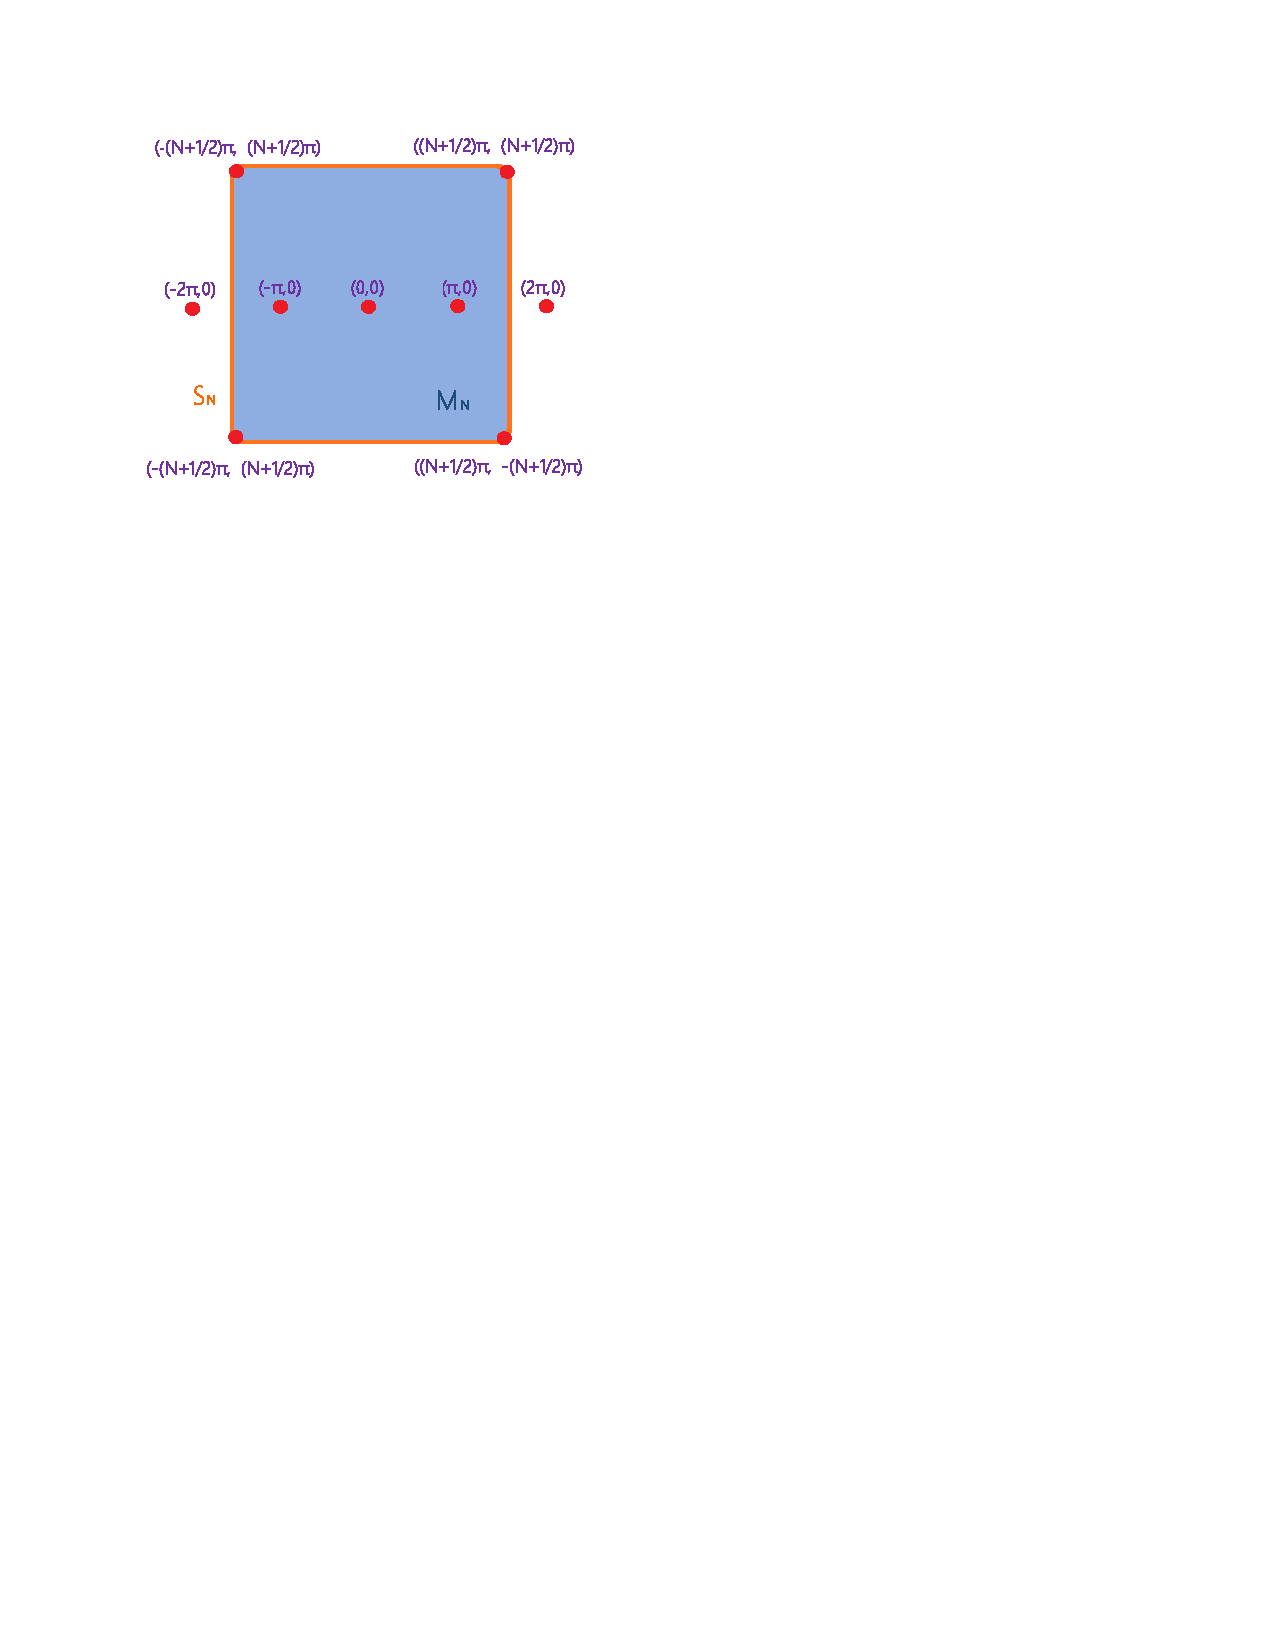
\includegraphics[scale=0.8]{MNSN.pdf}
\end{center}
Consider $M_N \in \Complex$ as described above. Note that for $z \in S_n \coloneqq \Bd(M_N)$,  we have $|\cot(z)|\leq 2$. Here we round the corners of $M_N$ to make it a $2$-manifold. Note that we have $|\frac{\cot(z)}{z^2}|\leq \frac{2}{N^2}$ on $S_N$. Then applying ML-estimate, we get the following:
\begin{align*}
\left| \int_{S_N}\frac{\cot(z)}{z^2}\, dz \right| \leq \frac{2}{N^2} \left( \pi (8N+4)\right)
\end{align*}
hence by Residue Theorem and ML-estimate, we have the following:
\begin{align*}
0&=\lim_{N\to \infty} \frac{1}{2\pi i}\int_{S_N}\frac{\cot(z)}{z^2}\, dz \\
&= \lim_{N\to \infty}\sum_{k=-N}^{N}Res\left( \frac{\cot(z)}{z^2}\, dz,\ k\pi\right) \\
&= \lim_{N\to \infty}\left( -\frac{1}{3}+ 2\sum_{k=1}^N \frac{1}{k^2 \pi^2}\right) \\
&= -\frac{1}{3}+2\sum_{k=1}^{\infty}\frac{1}{k^2 \pi^2}
\end{align*}
Rearranging we have:
\begin{align*}
\sum_{k=1}^\infty \frac{1}{k^2} = \frac{\pi^2}{6}
\end{align*}


\hfill\break\hfill\break
One can use the same technique as the example above to evaluate the following:
\begin{align*}
\sum_{k \in \Z \setminus F} \frac{P(k)}{Q(k)}
\end{align*}
with $P, Q$ being polynomials satisfying $\deg(Q) \geq \deg(P) + 2$, and $F$ is a finite subset of $\Z$. \\

One can show that we have the following holds:
\begin{align*}
\sum_{k \in \Z\setminus\{0\}}\frac{1}{k^p} = \begin{cases}2\sum_{k=1}^\infty \frac{1}{k^p} & p \text{ is even} \\ 0 & p\text{ is odd} \end{cases}
\end{align*}
\begin{defn}
For $p \in \Z$, $\zeta (p) = \sum_{k=1}^\infty \frac{1}{k^p}$ is the Riemann zeta function evaluated at $p$.
\end{defn}
\begin{thm}[Apery's Theorem]
$\zeta(3)$ is irrational. \hfill - Roger Apéry (1978)
\end{thm}
\begin{thm}
At least one of $\zeta(5)$, $\zeta(7)$, $\zeta(9)$, $\zeta(11)$ is irrational.  \hfill - W. V. Zudilin (2001)
\end{thm}
\hfill\break\hfill\break
Let $f:\Complex \to \Complex$ be a holomorphic function, let $z \in \Complex$, note here $(\zeta - z) \sin(\pi \zeta) = 0$ for $\zeta \in \Z\cup\{z\}$. Applying the Residue Theorem and proceed similar to what we did above, we get:
\begin{align*}
\int_{\zeta \in M_N}\frac{f(\zeta)\, d\zeta}{(\zeta - z) \sin(\pi \zeta)} = 2\pi i \left(\frac{f(z)}{\sin(\pi z)}+\sum_{k = -N}^{N} \frac{(-1)^k f(k)}{\pi (k-z)} \right)\tag{IN}
\end{align*}
For some well-defined $M_N \subseteq \Complex$. If $|f(z)|\leq C e^{\sigma |\Im(z)|}$ for constant $C$ and $0 < \sigma < \pi$, then $LHS $ of equation (IN) tends to $0$ when $N$ tends to $\infty$. Here we get:
\begin{align*}
\frac{f(z)}{\sin(\pi z) } = \sum_{k=-\infty}^{\infty}\frac{(-1)^{k+1}f(k)}{\pi (k - z)}
\end{align*} 
Rearranging we get:
\begin{align*}
f(z) = \sum_{k=-\infty}^{\infty} f(k) \frac{\sin(\pi (z-k))}{\pi (z-k)}
\end{align*}
That is, we can explicitly recover $f$ from $f|_{\Z}$, but we might not be able to do so if the condition $|f(z)|\leq C e^{\sigma |\Im(z)|}$ fails. For detains on information theory, check out Shannon's Theorem.

\newpage
\section[Winding Numbers]{\color{red}Winding Numbers\color{black}}
\begin{defn}
Let $M$ be compact oriented $1$-manifold without boundary in $\R^2\simeq \Complex$. We define the following function:
\begin{align*}
\mathbb{W}_M: \Complex\setminus M \to \Complex  \qquad z\mapsto \frac{1}{2\pi i}\int_{\zeta \in M} \frac{d\zeta}{\zeta -z}
\end{align*}
\end{defn}

In the settings Definition 40.0.0.0.1, let $M_1$, $M_2$, $\cdots$, $M_n$ denote the components of $M$, one can show that we have:
\begin{align*}
\frac{1}{2\pi i}\int_{\zeta \in M_j}\frac{d\zeta}{\zeta- z} = \frac{1}{2\pi} \left( \Delta_{M_j} \that{\text{arg}}(\zeta - z)\right)  \in \Z
\end{align*}
the term $ \Delta_{M_j} \that{\text{arg}}(\zeta - z)$ measures the total angle of the path $M_j$ winding around $z$, hence $\frac{1}{2\pi} \ \Delta_{M_j} \that{\text{arg}}(\zeta - z)$ is an integer and it measures the number of times $M_j$ winding around $z$. Here $\mathbb{W}_M(z)$ is called the winding number of $M$ with respect to $z$, which measures the total number of times the components of $M$ winding around $z$.\\


\note If $M$ is a compact connected oriented $1$-manifold without boundary in $\R^2\simeq \Complex$, then $M$ is diffeomorphic to $S^1$.\\

In general, for compact oriented $1$-manifold $M$ without boundary in $\Complex$, one can show that $\mathbb{W}_M(z) \in \Z$ for all $z \in \Complex$, and $\mathbb{W}_M$ is a continuous function on $\Complex \setminus M$, that is, $\mathbb{W}_M$ is constant on each component of $\Complex \setminus M$. \\

On the other hand, for $z \in \Complex$, we observe that $\mathbb{W}(z)$ tends to $0$ as $|z|$ tends to infinity. Then given $\epsilon>0$, there exists $R>0$ such that $\mathbb{W}_M(z) < \epsilon$ for $z \in \Complex$ that satisfies $|z|>R$, and hence $W_M(z) = 0$ on the component containing $\{z \in \Complex \mid |z| >R\}$, such component of $\Complex \setminus M$ is called unbounded component.\\


Let $M$ be an oriented connected compact $1$-manifold without boundary in $\Complex$, let $p \in M$. 
\begin{center}
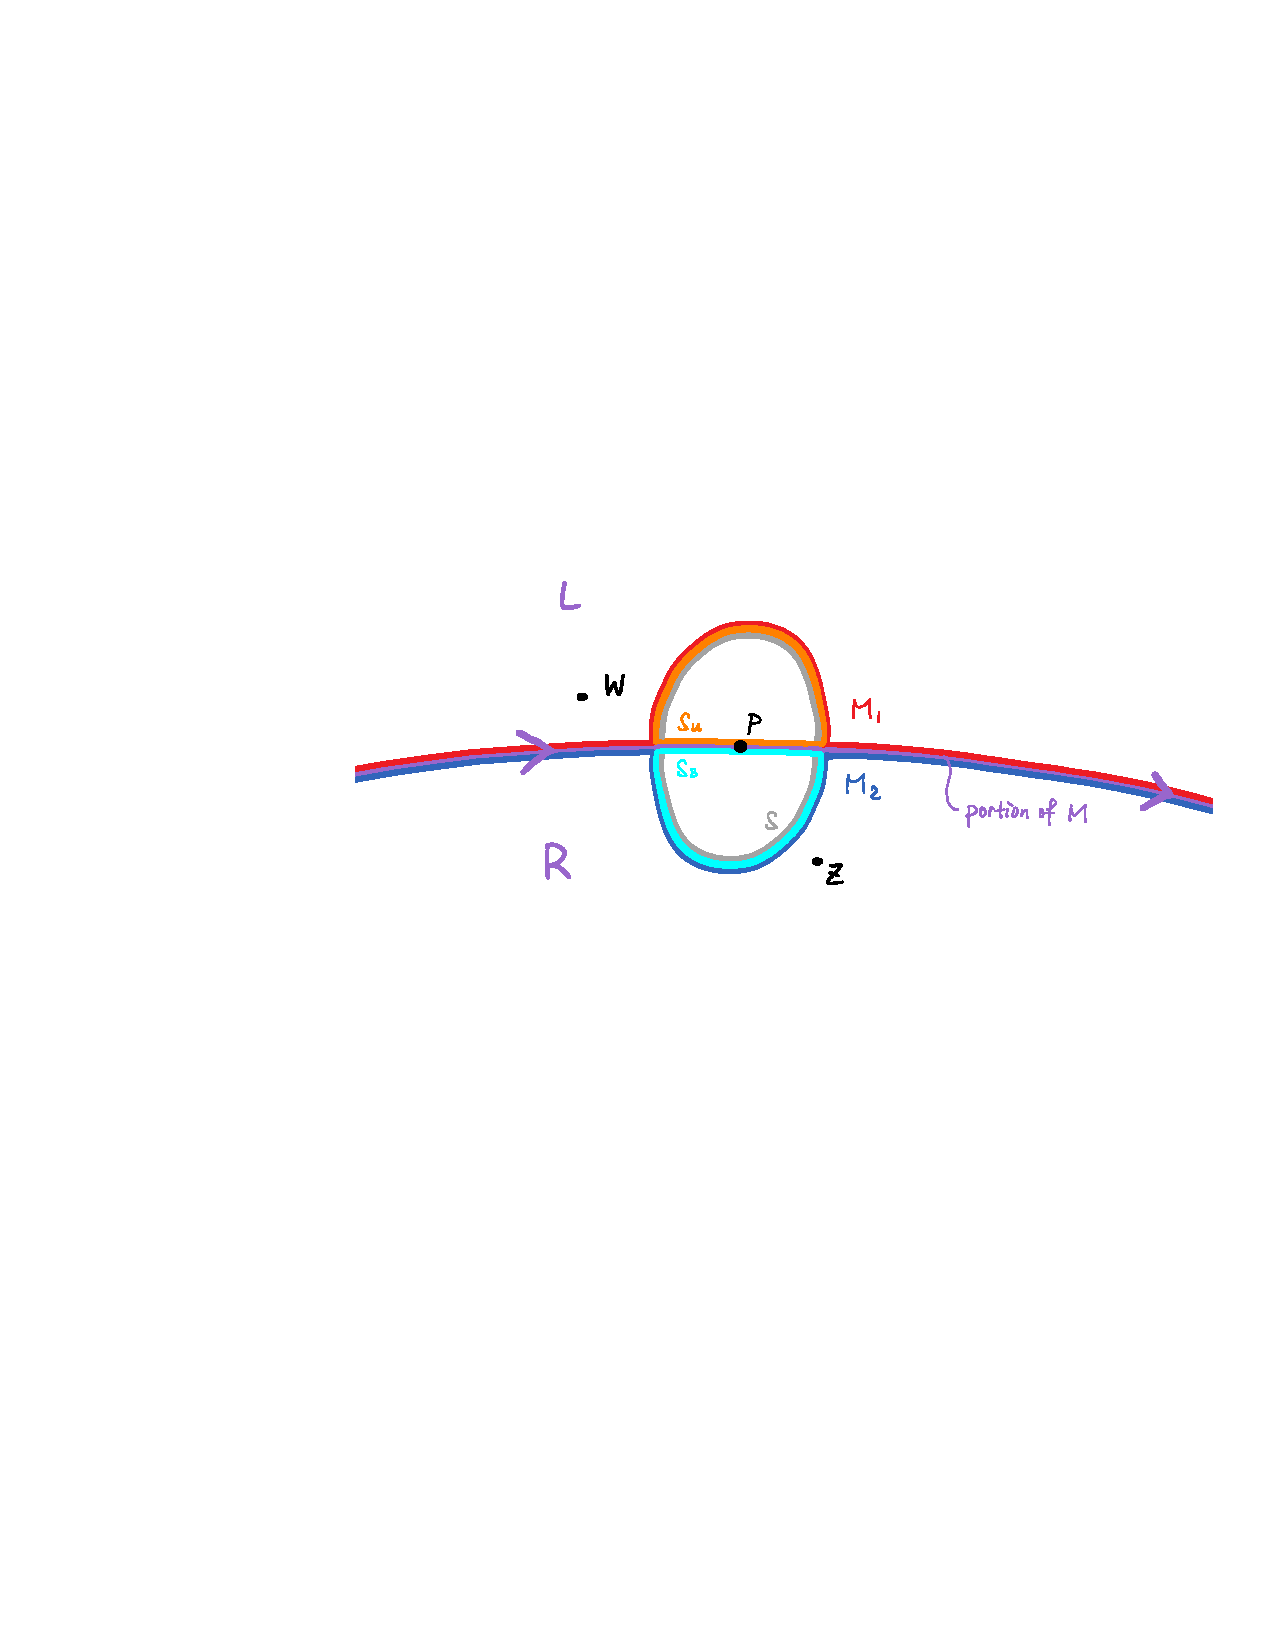
\includegraphics[scale=0.65]{winding.pdf}
\end{center}

From the figure,  by Cauchy Integral Theorem, we can write:
\begin{align*}
\mathbb{W}_{M}(z)  - \mathbb{W}_{M_1}(z) = \frac{1}{2\pi i}\int_{\zeta \in S_{u}} \frac{d\zeta}{\zeta - z} = 0 \qquad \Rightarrow \qquad \mathbb{W}_{M_1}(z) = \mathbb{W}_{M}(z) 
\end{align*}
similarly we have:
\begin{align*}
\mathbb{W}_{M}(w) - \mathbb{W}_{M_2}(w)  = \frac{1}{2\pi i}\int_{\zeta \in S_{b}} \frac{d\zeta}{\zeta - w} = 0 \qquad \Rightarrow \qquad \mathbb{W}_{M_2}(w) = \mathbb{W}_{M}(w) 
\end{align*}
Now we can write the following by following the orientation of $M$:
\begin{align*}
\mathbb{W}_{M}(z) - \mathbb{W}_{M}(w) = \mathbb{W}_{M_1}(z) - \mathbb{W}_{M_2}(w) =
\mathbb{W}_{M_1}(p) - \mathbb{W}_{M_2}(p) = -\frac{1}{2\pi i}\int_{\zeta \in S}\frac{d\zeta}{\zeta - p} =  -1
\end{align*}

\exercise There exists $U\subseteq \Complex$ containing $M$ such that $U \setminus M$ has two components $L,R$. Denote the winding number of $w \in L$ as $\mathbb{W}(L)$ and denote the winding number of $z \in R$ as $\mathbb{W}(R)$, we have: 
$$\mathbb{W}(L) = \mathbb{W}(R)+1$$

We conclude that, for compact connected $M$ without manifold boundary, $\Complex\setminus M$ has exactly $2$ components, and hence $\mathbb{W}_M(\Complex \setminus M) = \{0,1\}$ or $\{0,-1\}$. Reversing orientation of $M$ if needed, we have $\mathbb{W}_M(\Complex \setminus M) = \{0,1\}$. Here $\mathbb{W}_M^{-1}(1)$ is a connected open set forming the interior of a connected compact $2$-manifold, and we have $\Bd(\mathbb{W}_M^{-1}(1)) = M$. This result is known as Jordan Curve Theorem for differentiable case.\\

In general, let $M$ be a compact $1$-manifold without boundary in $\Complex$, not necessarily connected. One can show that $\mathbb{W}_M(\Complex \setminus M) $ is a finite subset of $Z$. On the other hand, for $j \in \Z\setminus \{0\}$, $X_j \coloneqq W_M^{-1}(j)$ is either $\emptyset$, or is the interior of a compact $2$-manifold in $\Complex$.\\

\begin{thm}[Residue theorem for Winding Numbers]
Let $M$ be a compact $1$-manifold without boundary in $\Complex$, let $K$ denote the union of the bounded components on $\Complex \setminus M$, let $U$ be an open subset of $\Complex$ containing $M\cup K$, let $\{z_1,z_2,\cdots, z_m\} \in U\setminus M$, and let $f$ be a function being holomorphic on the set $U \setminus \{z_1,z_2,\cdots, z_m\}$,  then we have:
$$\int_M f\, dz = 2\pi i \sum_{j=1}^m \mathbb{W}_M(z_j) \cdot Res(f\, dz, z_j)$$
\end{thm}
 


\newpage
\chapter{Geometry}
\setcounter{section}{40}
\section[The Isoperimetric Inequality]{\color{red}The Isoperimetric Inequality \color{black}}
Some problems related to infinite dimensional functional spaces make essential use of the fact that, the set of functions $C([a,b],\R^n)$ equipped with the metric defined by the following constitutes a complete normed vector space, or called a Banach space: $$n_{\sup}: C([a,b],\R^n) \to \R_{\geq 0} \qquad f \mapsto \max\{||f(t)||\ \mid a\leq t\leq b\}$$
Here $||f||_{\sup} \coloneqq n_{\sup}(f)$ for $f \in C([a,b],\R^n)$.
\hfill\break
\begin{defn}
The following set defines a set of periodic functions of $C^2$ type defined on $\R$:
$$C^2_{per}(\R, \R^2) \coloneqq \{ f \in C^2(\R,\R^2)\mid f(t+1) = f(t)\}$$ 
\end{defn}
\hfill\break

\exercise The set $C^2_{per}(\R, \R^2)$ equipped with the norm $n:C^2_{per}(\R, \R^2) \to \R_{\geq 0} \ \ \ f\mapsto ||f|| $ constitutes a Banarch space, where for $f \in C^2_{per}(\R, \R^2)$, we define:
$$||f|| \coloneqq \max\{||f(t)||\ \mid 0 \leq t\leq 1\} + \max\{||f'(t)||\ \mid 0 \leq t\leq 1\} + \max\{||f''(t)||\ \mid 0 \leq t\leq 1\}$$

\begin{defn}
For $f\in C^2_{per}(\R, \R^2)$, we denote: 
$$f:\R \to \R^2 \ \ \ t\mapsto \bmat{x(t)\\y(t)}$$ 
Here we define the following function:
$$l:C^2_{per}(\R, \R^2) \to \R \ \ \ f\mapsto \int_0^1 \sqrt{(x'(t))^2 + (y'(t))^2}\, dt$$ 
\end{defn}

\remark Let $f\in C^2_{per}(\R, \R^2)$. \\
$l(f)$ gives the $1$-volume of a parametrized $1$-manifold parametrized by $f$. \\

\note For $f\in C^2_{per}(\R, \R^2)$, $l(cf) = |c| \cdot l(f)$ for $c \in \R$ and $f\in C^2_{per}(\R, \R^2)$. 
\newpage

\begin{defn}
For $h:C^2_{per}(\R, \R^2) \to \R$, we define the directional derivative of $h$ at $f$ in the direction of $g$ as the following, if exists:
\begin{align*}
h'(f;g) \coloneqq \lim_{u \to 0}\frac{h(f+ug) - h(f)}{u}
\end{align*}
\end{defn}

Now we get the following for $f,g \in C^2_{per}(\R, \R^2)$: 
$$l'(f;g) \coloneqq \lim_{u \to 0}\frac{l(f+ug) - l(f)}{u} = \left(\frac{d}{du}(l(f+ug))\right)|_{u = 0}$$
\note For notation, $(\mu(u))|_{u=0}$ denote the function $\mu(u)$ evaluated at $u = 0$.\\

In this section, for notation, for $g,f \in C^2_{per}(\R, \R^2)$, we denote:
\begin{align*}
g:\R \to \R^2 \ \ \ t\mapsto \bmat{p(t)\\ q(t)} \qquad \qquad \qquad f:\R \to \R^2 \ \ \ t\mapsto \bmat{x(t)\\y(t)}
\end{align*}
Then we can write:
\begin{align*}
l(f+ug) = \int_0^1 \sqrt{\lr{x'(t) + up'(t)}^2 + \lr{y'(t) + uq'(t)}^2}\, dt
\end{align*}
By Leibniz Integral Rule, we get:
\begin{align*}
l'(f;g) &= \int_0^1 \left(\frac{\partial}{\partial u}\sqrt{\lr{x'(t) + up'(t)}^2 + \lr{y'(t) + uq'(t)}^2}\right)|_{u=0} \, dt   \\
&= \int_0^1 \left(\frac{x'(t)p'(t)+y'(t)q'(t)+u(p'(t))^2+u(q'(t))^2}{\sqrt{\lr{x'(t) + up'(t)}^2 + \lr{y'(t) + uq'(t)}^2}}\right)|_{u=0} \, dt \\
&= \int_0^1 \frac{x'(t)p'(t)+y'(t) q'(t)}{\sqrt{(x'(t))^2+(y^2(t))^2}}\, dt \tag{LO}
\end{align*}
Equation (LO) is valid if $(x'(t))^2+(y^2(t))^2 \neq 0$ for all $t$.

\begin{defn}
Let $U$ be a subset of $\R^k$, let $f:U \to \R^n$ be a function.\\ 
$f$ is called an immersion provided that $Df(\vec{x})$ is injective for all $\vec{x}\in U$. \\
$f$ is called a submersion provided that $Df(\vec{x})$ is surjective for all $\vec{x}\in U$.  
\end{defn}

In this section, for notation, we denote $V = C_{per}^2 (\R,\R^2)$. The image of $f \in V$ might be a compact connected $C^2$ parametrized $1$-manifold without boundary, but it depends on whether $f$ is injection on $[0,1)$. We denote $U_1 = \{ f\in V \mid Df(\vec{x}) \neq 0\}$, for $f \in U_1$, we see that $f$ is an immersion. Note that $U_1$ is an open subset of $V$, and $l'(f;g)$ exists for $f \in U_1$ and $g \in V$.\\

\exercise $l'(f;f) = l(f)$ for $f \in U_1$. \\
\exercise $l$ is differentiable at each $f \in U_1$. \\
\exercise $l'(f; cg) = c\, l'(f;g)$ for $c \in \R$, $f \in U_1$, and $g \in V$.\\

\begin{defn}
$$a:V \to \R \ \ \ f\mapsto \frac{1}{2}\int_0^1 (\,x(t)\,y'(t) - x'(t)\,y(t)\,)\, dt$$
\end{defn}
\note Denote $Y = f([0,1])$ for $f \in V$, we have:
\begin{align*}
a(f) = \frac{1}{2}\int_{Y_f} x\, dy - y\, dx 
\end{align*}
\note We have $a(cf) = c^2a(f)$ for $f \in V$ and $c \in \R$.\\

In this section, for notation, denote $U_2 \coloneqq \{ f \in U_1 \mid f\text{ is injective on }[0,1)\}$. Note that $U_2$ is an open subset of $U_1$. For $f\in U_2$, $f$ parametrizes manifold without boundary.\\

\note $f \in U_2$ implies $f(\R)  = \partial \Omega$, where $\Omega$ is a compact $2$-manifold in $\R^2$. We can write:
\begin{align*}
a(f) =\pm  \frac{1}{2}\int_{\partial \Omega} x\, dy - y\, dx = \pm \int_{\Omega} dx \wedge dy =\pm (\,2\text{-volume of }\Omega\,)
\end{align*} 

Define $U_3 = \{ f\in U_2 \mid a(f) >0 \}$, in which case $a(f)$ gives the $2$-volume of $\Omega$ for $f \in U_3$ and we have $f(\R) = \partial \Omega$. \\


\exercise \\
For $f,g \in V$, by Integration by Part and noticing that $f,g$ are periodic, one can get:
\begin{align*}
a'(f;f) = 2a(f) \qquad\qquad
a'(f;g) &= \frac{1}{2} \int_0^1 xq' - x'q - yp' + y' p \\
&= \int_0^1 xq' - yp' = \int_0^1 y'p - x'q 
\end{align*}

\exercise $a$ is differentiable on $V$. \\

\note Here we have:
\begin{align*}
\sup a(U_j) = \infty  = \sup l(U_j) \qquad\qquad\qquad\qquad \inf a(U_j) = 0 = \inf l(U_j)
\end{align*}
Now consider the following with $\alpha,\beta \in \R$:
\begin{align*}
\frac{a^\alpha (cf)}{l^\beta (cf)} = |c|^{2\alpha - \beta} \frac{a^\alpha(f)}{l^{\beta}(f)} \tag{RT}
\end{align*}
the supremum of infimum of (RT) over $U_j$ is still $\infty$ and $0$ respectively unless $\beta = 2\alpha$. \\

\begin{defn}
$$h:U_1 \to \R \qquad f \mapsto \frac{a(f)}{l^2(f)}$$
\end{defn}

\newpage
By results derived above, for $f \in U_1$, $a'(f;g) = 0$ for all $g \in V$ if and only if we have $x'(x) = y'(x) = 0$ for all $x \in U_1$, if and only if $f$ is a constant function. Note that we also have, for $f \in U_1$ and $g \in V$, the following holds:
\begin{align*}
l'(f;g) = \int_0^1 \frac{x'p'+y'q'}{\sqrt{(x')^2 + (y')^2}} = \int_0^1 (y'p - x'q) \frac{x'y'' - x'' y'}{\lr{(x')^2 + (y')^2}^{3/2}}
\end{align*}
Here $\kappa_f \coloneqq \frac{x'y'' - x'' y'}{\lr{(x')^2 + (y')^2}^{3/2}} $ is know as the curvature of $f$. \\

Here we see that, for $f \in U_1$, $l'(f;g) = 0$ for all $g \in U_1$ if and only if we have $y'(x'y''-x''y') = 0 = x'(x'y''-x''y')$, if and only if $x'y'' - x'' y' = 0$. If $x',y'$ are linearly dependent, then $x'y'' - x''y' = 0$ is guaranteed by Math 396 HW3 Q3, if $x'y'' - x''y' =0$ holds on $U_1$, then $x', y'$ are linearly dependent. \\

\note If $x'$ and $y'$ are linearly dependent, then $f(\R)$ is a subset of a line in $\R^2$. \\

For $f,g \in U_1$, we can write the following:
\begin{align*}
h'(f;g) = \frac{l(f)a'(f;g)-2a(f)l'(f;g)}{l^3(f)}
\end{align*} 

\exercise $h'(f,f) = 0$ for all $f \in U_1$\\

For $f \in U_1$, here we see that $h'(f;g) = 0$ for all $g \in V$ if and only if we have:
\begin{align*}
a'(f;g) = \frac{2a(f)}{l(f)}l'(f;g) \tag{*}
\end{align*}
for all $g \in V$. \\

Suppose on the other hand,for $f \in U_1$, we get $a'(f;g) = \lambda l'(f;g)$ for all $g \in V$ for some constant $\lambda$. Set $g = f$, from result derived above we have $2a(f) = \lambda l(f)$, then $\lambda = \frac{2a(f)}{l(f)}$, in which case we see that (*) holds. We conclude that $h'(f;g) = 0$ for all $g$ if and only if there exists some $\lambda$ such that $a'(f;g) = \lambda l'(f;g)$ for all $g$, if and only if $f$ satisfies Lagrange condition for maximizing or minimizing $a$ with $l$ being a constant, if and only if $f$ satisfies Lagrange condition for maximizing or minimizing $l$ with $a$ being a constant. \\

Also, for $f \in U_1$, and constant $\lambda$, $a'(f;g) = \lambda l'(f;g)$ for all $g \in V$ if and only if we have:
\begin{align*}
\int_0^1 (y'p - x'q) = \lambda \int_0^1 (y'p - x'q)\frac{x'y''-x''y'}{((x')^2 + (y')^2)^{3/2}} \qquad \forall p,q,\ s.t.\ g\in V \tag{**}
\end{align*}
Equation (**) implies that we have:
\begin{align*}
\frac{1}{\lambda} = \frac{x'y'' - x''y'}{((x')^2 + (y')^2)^{3/2}} = \kappa_f =\text{curvature of }f 
\end{align*}
In general curvature of $f$ is a function. For $f \in U_1$, by Math 396 HW11, if $\kappa_f $ is a constant, then $f(\R)$ is contained in a circle of radius $\frac{1}{\kappa_f} = \lambda$, or $f(\R)$ is a line with $\kappa_f = 0$. \footnote{Here $f(\R)$ are called clircles} \\

Here if $\kappa_f$ is a nonzero constant, $f$ is a critical point of $h$ as we have $\frac{1}{\lambda}$ being constant, and equation (**) gives rise to a form of Lagrange-Euler Equation, solving for the critical points of $h$.\\

Here if $f$ is a critical point of $h$, we get the following:\\
If $f\in U_3$, $f$ winds once forward on a circle each period.\\
If $f \in U_2 \setminus U_3$, $f$ winds once backward on a circle each period.\\
If $f \in U_1 \setminus U_2$, then $f$ goes around a circle multiple times each period. \\

\remark Many important PDE and ODE come from Lagrange-Euler Equation. For examples of applications of the Euler-Lagrange Equation of the form rising from equation (**), check out \textit{Chapter 3 - Lagrangian and Hamiltonian Dynamics} in the text \textit{Class Note: Physics 401 - Classical Mechanics}, transcribed by Jinyan Miao in Winter 2022. The course Physics 401 at the University of Michigan in Winter 2022 was taught by Professor Bing Zhou.\\

\note The critical points for $h$ in $U_3$ are circles. If $f\in U_3$ is a critical point for $h$, and $f$ traces out a circle of radius $r$, then we have: 
$$h(f) = \frac{\pi r^2}{(2\pi r)^2} = \frac{1}{4\pi}$$

\hfill\break
\begin{thm}[Isoperimetric Inequality]
Let $\Omega$ be a compact connected $2$-manifold in $\R^2$ with $\partial \Omega$ being connected, we have: 
$$\text{area}(\Omega) \leq \frac{1}{4\pi}\left( \text{length}(\partial \Omega)\right)^2$$ 
with $\text{area}(\Omega) = \frac{1}{4\pi}\left( \text{length}(\partial \Omega)\right)^2$ holds if and only if $\Omega$ is a disk.\\ Here $\text{area}(\Omega)$ is the $2$-volume of $\Omega$, and $\text{length}(\partial \Omega)$ is the $1$-volume of $\partial\Omega$.
\end{thm}

\hfill\break
Let $\Omega$ be a oriented compact connected $2$-manifold in $\R^2 \simeq \Complex$, let $\vec{N}$ be the unit normal vector field of $\partial \Omega$ corresponding to the induced orientation of $\partial \Omega$. One can show that there exists some $\epsilon_0>0$ such that the function $\Psi_\epsilon :\partial \Omega \to \R^2 \ \ \ \vec{z} \mapsto \vec{z} + \epsilon \vec{N}(\vec{z})$ satisfies the following conditions:
\begin{enumerate}[topsep=3pt,itemsep=-1ex,partopsep=1ex,parsep=1ex]
\item $\Psi_{\epsilon} (\partial \Omega) \cap \bar{\Omega} = \emptyset $ for $0<\epsilon\leq \epsilon_0$
\item for $0 < \epsilon \leq \epsilon_0$ and $z \in \Omega$, we have:
\begin{align*}
\frac{1}{2\pi i}\int_{\zeta \in \Psi_{\epsilon}(\partial \Omega)} \frac{d\zeta}{\zeta - z} = 1
\end{align*}
\item $l(\Psi_{\epsilon}(\partial \Omega))$ tends to $l(\partial \Omega)$ as $\epsilon $ tends to $0$. 
\end{enumerate} 

\newpage
\begin{thm}
Let $\Omega$ be a compact $2$-manifold in $\R^2$, we have the following holds:
$$\text{area}(\Omega) \leq \frac{1}{4\pi}\left( \text{length}(\partial \Omega)\right)^2$$
\end{thm}
\begin{proof}
Here we can write:
\begin{align*}
\text{area}(\Omega) = \int_{\Omega} dx\wedge dy &= \int_{\Omega} \frac{i}{2}\, dz \wedge d\bar{z}\\
&= \int_{z \in \Omega}\left( \frac{1}{2\pi i}\int_{\zeta \in \Psi_{\epsilon}(\partial \Omega)} \frac{d\zeta}{\zeta - z} \frac{i}{2}\right)\, dz \wedge d\bar{z} \\
&= \frac{1}{4\pi}\int_{z\in \Omega}\left(\int_{\zeta \in \Psi_{\epsilon}(\partial \Omega)} \frac{d\zeta}{\zeta - z} \right) dz\wedge d\bar{z}\\
&= \frac{1}{4\pi}\int_{\zeta \in \Psi_{\epsilon}(\partial \Omega)}\left( \int_{z \in \Omega} \frac{dz \wedge d\bar{z}}{\zeta - z}\, \right)d\zeta \\
&= \frac{1}{4\pi}\int_{\zeta \in \Psi_{\epsilon}(\partial \Omega)}\left( \int_{z \in \Omega} d\left(\frac{\bar{\zeta}-\bar{z}}{\zeta - z}\,dz\right)\, \right)\,d\zeta \\
&= \frac{1}{4\pi} \int_{\zeta \in \Psi_\epsilon(\partial \Omega)} \left( \int_{z\in \partial\Omega} \frac{\bar{\zeta} - \bar{z}}{\zeta - z}\, dz\right)\, d\zeta
\end{align*}
Note here we have $\left|\left|\frac{\bar{\zeta} - \bar{z}}{\zeta - z} \right|\right|  = 1$, and area is non-negative, then we get:
\begin{align*}
\text{area}(\Omega) = \frac{1}{4\pi}\left| \int_{\zeta \in \Psi_\epsilon(\partial \Omega)} \left( \int_{z\in \partial\Omega} \frac{\bar{\zeta} - \bar{z}}{\zeta - z}\, dz\right)\, d\zeta \right| \tag{AM}
\end{align*}
Applying ML-estimate for both integrals in equation (AM), we get the following:
\begin{align*}
\text{area}(\Omega) \leq \frac{1}{4\pi} l(\partial \Omega) l(\Psi_{\epsilon} (\partial \Omega)) \tag{AO}
\end{align*}
Let $\epsilon$ in equation (AO) tends to $0$, the result follows.
\end{proof}

\newpage
\section[Riemannian Metrics]{\color{red}Riemannian Metrics\color{black}}
Consider $f \in C^1(U,\R)$ where $U$ is an open subset of $\R^2$, let $M$
be $Graph(f) \subseteq \R^3$, let $Y$ be a parametrized $1$-manifold in $M$ parametrized by the following function:
\begin{align*}
\eta: V \to M \qquad t\mapsto \bmat{x(t)\\ y(t) \\ f\left(\bmat{x(t)\\y(t)}\right)}
\end{align*}
where $V=[a,b]\subseteq \R$, and $x,y$ are scalar-valued functions defined on $V$.

In such setting one can show that we get:
\begin{align*}
\text{le}&\text{ngth}\left(Y_{\eta}\right) \\
&= \int_a^b \sqrt{\alpha\left(\bmat{x\left(t\right)\\y\left(t\right)}\right)\left(x'\left(t\right)\right)^2 + 2\beta\left(\bmat{x\left(t\right) \\ y\left(t\right)}\right) x'\left(t\right) y'\left(t\right) + \gamma\left(\bmat{x\left(t\right) \\ y\left(t\right)}\right) \left(y'\left(t\right)\right)^2 }\, dt
\end{align*}
where $\alpha = 1+\left(D_1f\right)^2$, $\beta = D_1f \cdot D_2f$, $\gamma = 1+\left(D_2f\right)^2$. Note here we have:
\begin{align*}
\alpha\left(\bmat{x\left(t\right)\\y\left(t\right)}\right)\left(x'\left(t\right)\right)^2 + 2\beta\left(\bmat{x\left(t\right) \\ y\left(t\right)}\right) x'\left(t\right) y'\left(t\right) + \gamma&\left(\bmat{x\left(t\right) \\ y\left(t\right)}\right) 
\left(y'\left(t\right)\right)^2  \\
&= \bmat{x'\left(t\right) & y'\left(t\right)}\bmat{\alpha &\beta \\ \beta & \alpha} \bmat{x'\left(t\right) \\ y'\left(t\right)}
\end{align*}
which is positive as length must be positive, and the following matrix is always symmetric and positive with the set of eigenvalues $\{1, 1+(D_1f)^2 + (D_2f^2)\}$:
$$\bmat{\alpha &\beta \\ \beta & \alpha}$$  

\hfill\break
\begin{defn}
$\text{Symm}(k)$ denotes the set of $k\times k$ symmetric matrix. 
\end{defn}
\note $\text{Symm}(k)$ defines the space of symmetric $2$-tensors on $\R^k$. 

\begin{defn}
$\text{Pos}(k)$ is the set of positive symmetric $k\times k$ matrix.
\end{defn}
\note $\text{Pos}(k)$ is an ope subset of the set of symmetric $k\times k$ matrix.\\

\begin{defn}
Let $A$ be an open subset of $\R^k$. A Riemannian metric $G$ on $A$ is a smooth function defined by $G:A \to \text{Pos}(k)$. Given $\psi\in C^2([a,b],A)$, we define the $G$-length of $Y_\psi$, or the length of $Y_{\psi}$ in $G$ metric, as the following: 
$$l_G(Y_{\psi}) \coloneqq \int_a^b \sqrt{\psi'(t)^T \cdot G(\psi(t))\cdot \psi'(t)}\, dt$$
\end{defn}

\newpage
\begin{thm}[John Forbes Nash Jr. (1956), Mikhael Gromov (1986)]
Let $A$ be an open subset of $\R^k$. Let $G:A \to \text{Pos}(k)$ be a Riemannian metric on $A$. There exists diffeomorphism $\psi : A \to X$, where $X$ is a $k$-manifold in $\R^{k^2 + 10k +3}$ such that, for all $\phi\in C^2([a,b],A)$, we have the following holds:
$$ l_G(Y_\phi) = l(Y_{\psi \circ \phi})$$
\end{thm}
Similarly, let $A$ be an open subset of $\R^k$, there exists $\psi : A \to \R^{k+1}$ such that, for all $\phi\in C^2([a,b],A)$, we have $ l_G(Y_\phi) = l(Y_{\psi \circ \phi})$. Conversely, for $A,U \subseteq \R^k$ with $A \subseteq U$, given a coordinate patch $\psi: U \to V$, then there exists Riemannian metric $G$ on $U$ such that $ l_G(Y_\phi) = l(Y_{\psi \circ \phi})$ for all $\phi \in  C^2([a,b],A)$.\\

\example
Consider $A\subseteq \R^2$, define a Riemannian metric $G$ by the following:
\begin{align*}
G:A\to \text{Pos}(2) \qquad (x,y)\mapsto\frac{4}{(1+x^2 + y^2)^2}\, I
\end{align*} 
where $I$ is the identity matrix, define a function $\psi:\R^2 \to S^2\setminus \{\vec{e}_3\}$ by setting: 
$$\psi(x,y) = \frac{1}{x^2 + y^2 + 1}(2x,\ 2y,\ x^2 +y^2 -1)$$ 
$\psi$ defines a diffeomorphism. \\

\hfill\break
For $A = \R^2$, and graph curves $\phi_f : x \mapsto (x,f(x))$, suppose we have $\that{a},\that{b} \in \R$, we set: 
$$E = \{ f\in C^2([a,b], \R)\mid f(a) = \that{a}, f(b) = \that{b}\}$$ Consider $L:E \to \R \ \ \ f\mapsto l_G(Y_{\phi_f})$, we are interested in the critical points for $L$.\\

Here $E$ is a space of functions, in particular, $E$ is an affine subset of $C^2([a,b],\R)$, then there exists an associate vector space $E' \coloneqq \{f \in C^2([a,b], \R) \mid f(a) = 0 = f(b)\}$. \\

To find critical points of $L$, one can apply the two constraints $f(a) = 0 = f(b)$ and use the Lagrange Multiplier method, or one can look for $f \in E$ solving $L'(f;g) = 0$ for $g \in E'$. Here we write:
\begin{align*}
L'(f;g) &= \left(\frac{d}{ds} \left(L (f+sg)\right)\right)|_{s= 0} \\
&= \left.\frac{d}{ds} \left(\int_a^b \sqrt{\bmat{1 & f'+sg'}\bmat{\alpha\bmat{t \\ f+sg}&\beta\bmat{t \\ f+sg}\\\beta\bmat{t \\ f+sg}&\alpha\bmat{t \\ f+sg}}\bmat{1 \\ f'+sg'}} \right)\right|_{s= 0}
 \end{align*}
By Leibniz Integral Rule, boundary conditions, and Integration by Parts, one can show that we have the following holds:
\begin{align*}
L'(f;g) = \int_a^b \left(g\cdot \eta_1(f,f';t) + g'\cdot \eta_2(f,f';t)\right) \, dt = \int_a^b g\cdot \left(\eta_1(f,f';t) - (\eta_2(f,f';t))'\right) \, dt
\end{align*}
Here $f$ is a critical point for $L|_E$ if and only if $\eta_1(f,f';t) = (\eta_2(f,f';t))'$, if and only if we have the following:
\begin{align*}
f'' = \eta(f,f';t) \tag{*}
\end{align*} 
if and only if we have the following:
\begin{align*}
\bmat{f \\ f'}' = \bmat{f' \\ \eta(f,h;t) }\tag{**}
\end{align*}
for some functions $\eta,\eta_1,\eta_2$ which can be computed. \\


Fundamental Theorem of ODEs implies that one can uniquely solve $(**)$ under condition $f(x_0) = y_0$ and $f'(x_0) = v_0$, which is equivalent to solve $(*)$ with condition $f(x_0) = y_0$ and $f'(x_0) = v_0$.\\

\example\\
Let $A \subseteq \R^2$, consider a Riemannian metric $G$ defined by the following: 
$$G:A \to \text{Pos}(2) \qquad (x,y)  = I$$ 
where $I$ is the $2\times 2$ identity matrix, and here $G$ defines the Euclidean metric. \\
For $f \in \{ g\in C^2([a,b], \R)\mid g(a) = \that{a}, g(b) = \that{b}\}$, we can write the following with Leibniz Rule and Integration by Parts:
\begin{align*}
L'(f,g) 
&= \left( \frac{d}{ds} \int_a^b \sqrt{1 + (f'+sg')^2}\, dt \right)|_{s= 0} \\
&= \int_a^b \frac{f'g'}{\sqrt{1+(f')^2}}\, dt = -\int_a^b \frac{f'' g}{\sqrt{(1+(f')^2)^{3/2}}}\, dt
\end{align*}
$$\frac{f''}{\sqrt{(1+(f')^2)^{3/2}}} \coloneqq \text{ is called the curvature of graph curves }\text{Graph}(f)$$
Here $f$ is a critical point for $L$ if and only if $f'' = 0$ if and only if $\text{Graph}(f)$ is affine. \\

\exercise Given $Y_{\phi}$ parametrized by $\psi\in C^2([a,b],A)$, where $A$ is an open set, rotating $Y_{\phi}$ does not change the value of $l_I(Y_{\phi})$, where $I$ is the identity matrix.\\ 

For Riemannian matrix $G = I$, we have shown that affine graph curves minimize $L$. Now consider joining point $(a,\that{a})$ to point $(b,\that{b})$ by a curve, here we can use rotation of the curves to reduce to the case where $\that{b} = \that{a}$. Let $\phi$ be a function in $C^1([a,b],\R^2)$. For $t\in [a,b]$, let $\phi(t) = (x(t), y(t))$, with $\phi(A) = (a,\that{a})$ and $\phi(B) =(b,\that{b}) = (b,\that{a})$. We write:
\begin{align*}
l_I(Y_{\phi}) = \int_A^B \sqrt{(x')^2 + (y')^2} \geq \int_A^B \sqrt{(x')^2} = \int_A^B |x'| \geq \int_A^B x' = x(B) - x(A) = b-a
\end{align*}
Note here $b-a$ gives the length, under the Riemannian metric $G = I$, of a straight line segment joining the point $(a,\that{a})$ to the point $(b,\that{b})$.\\

\example (Poincare Metric)\\
Let $A = \mathbb{H}_+^2$, consider the Riemannian metric $G$ defined by the following:
\begin{align*}
G:A \to \text{Pos}(k) \qquad \bmat{x\\y}\mapsto \bmat{\frac{1}{y^2} & 0 \\ 0 & \frac{1}{y^2}}
\end{align*}
Here $G$ here is called the Poincare metric, or hyperbolic metric. \\
For $\phi\in C^1([a,b], \R^2)$, denote $\phi(t) = (x(t),y(t))$, here we can write:
\begin{align*}
l_G(Y_{\phi}) = \int_a^b \frac{\sqrt{(x')^2 + (y')^2}}{y} = \int_a^b \frac{dV}{y}
\end{align*}
For technical reasons, we will focus on sideways graphs, that is, we write:
\begin{align*}
\phi:C^1([a,b], \R \qquad y \mapsto \bmat{f(y) \\ y}
\end{align*}
then we have:
\begin{align*}
L(f) = \int_a^b \frac{\sqrt{1+(f'(y))^2}}{y}\, dy
\end{align*}
Using Leibniz Rule, and Integration by Parts, we get:
\begin{align*}
L'(f;g) = \int_a^b \frac{f'(y) g'(y)}{\sqrt{1+ (f'(y))^2}}\, dy = \int_a^b  \frac{-y f''(y) + f'(y) + (f'(y))^3}{y(1+(f'(y))^2)^{3/2}}g(y)\, dy
\end{align*}
for $f$ to be a critical point for constrained $L$, we must have the following holds:
\begin{align*}
L'(f;g) = 0 \ \ \forall g \in E' \qquad \iff \qquad yf''(y) = f'(y) + (f'(y))^3  \tag{C}
\end{align*}
Equation (C) holds if and only if, by HW12, $Y_{\phi}$ is contained in, a circle centered on $x$-axis, or a vertical line. These are lines for Poincare's model of Bolyai-Lobachevsky non-Euclidean geometry. Any points $\mathbb{H}_+^2$ are joint by exactly one Poincare line. \\

\begin{defn}
We denote the Poincare length of a curve $Y_{\phi}$ as $l_{Poin}(Y_\phi)$.
\end{defn}

\begin{thm}
The followings minimize Poincare length among curves with the same end points:
\begin{enumerate}[topsep=3pt,itemsep=-1ex,partopsep=1ex,parsep=1ex]
\item Vertical segment in $\mathbb{H}_+^2$
\item Arc in $\mathbb{H}_+^2$ of circle centered on $x$-axis
\end{enumerate}
\end{thm}
\begin{proof}
Assume endpoints of the vertical segment as $(x_1, y_1)$, $(x_1,y_2)$ with $y_1 < y_2$, and such vertical line segment is parametrized by $\phi$ defined by the following:
\begin{align*}
\phi : I \to \mathbb{H}_+^2 \qquad t\mapsto \bmat{x(t) \\ y(t)}
\end{align*}
Note here we have the following holds:
\begin{align*}
l_{\text{Poin}}\left(Y_{\phi}\right) = \int_I \frac{\sqrt{(x')^2 + (y')^2}}{y} \geq \int_I \frac{\sqrt{(y')^2}}{y} =\int_I \frac{|y'|}{y} \geq \int_I \frac {y'}{y} = \Delta_I \ln(y) = \ln\left( \frac{y_2}{y_1}\right)
\end{align*}
To complete the proof of Theorem 42.3, we will make use of the following exercise:\\

\newpage
\exercise The following diffeomorphisms of $\mathbb{H}_+^2$ preserve $l_{\text{Poin}}$:
\begin{enumerate}[topsep=3pt,itemsep=-1ex,partopsep=1ex,parsep=1ex]
\item $f: \mathbb{H}_+^2 \to \mathbb{H}_+^2 \ \ \ (x,y) \mapsto (x+a, y)$ for $a \in \R$\\
which is equivalent to the holomorphic function $h:\Complex \to \Complex \ \ \ z\mapsto z+a$
\item $f: \mathbb{H}_+^2 \to \mathbb{H}_+^2\ \ \ (x,y) \mapsto (\lambda x, \lambda y)$ with $\lambda>0$\\
which is equivalent to the holomorphic function $h:\Complex \to \Complex \ \ \ z\mapsto \lambda z$
\item $f: \mathbb{H}_+^2 \to \mathbb{H}_+^2\ \ \ (x,y) \mapsto (-\frac{x}{x^2+y^2} , \frac{y}{x^2 + y^2})$\\
which is equivalent to holomorphic $h: \Complex  \to \Complex  \ \ \ z\mapsto 1/z$ for $z \in \Complex$
\end{enumerate}

\note The group of diffeomorphism generated by (1), (2), and (3) is given by:
\begin{align*}
\left\{f:\Complex \to \Complex \ \ \ z\mapsto \frac{az+b}{cz+d} \mid a,b,c,d,\in \R , ad-bc = 1\right\} = SL(2,\R) / \{\pm I\}
\end{align*}
which is the group of all orientation preserving isometries of the metric space: 
$$(\mathbb{H}_+^2, \text{Poincare metric})$$ 
and $SL(2,\R) / \{\pm I\}$ is the group of holomorphic bijection from $\mathbb{H}_+^2$ to $\mathbb{H}_+^2$.\\

Here we note that (3) maps the vertical line $x=1$ to $(x+\frac{1}{2})^2 + y^2 = \frac{1}{4}$, and (1) and (2) maps $(x+\frac{1}{2})^2 + y^2 = \frac{1}{4}$ to any possible circles centered on the $x$-axis.\\

Finally, to complete the proof of Theorem 42.3, we will make use of the following exercise:\\

\exercise \\
Any $(x_1,y_2),(x_2,y_2) \in \mathbb{H}_+^2$ lie on such a circle, or a vertical line segment described above. \\

This completes the proof of Theorem 42.3.
\end{proof}


\hfill\break
\hfill\break
\remark Here we defined the Riemannian metric to be $G:A \to \text{Pos}(k)$ where $A$ is an open subset of $\R^k$. Given a Riemannian metric, the usual metric, or the point metric for points in $A$, that we have defined previously is induced from such Riemannian metric, which is given by the following:
\begin{align*}
d:A \times A \qquad (\vec{p},\vec{q}) \mapsto \inf \left\{l_G(Y_{\phi}) \mid \phi \in C_{pw}^1([a,b],A),\ \phi(a) = \vec{p}, \ \phi(b) = \vec{q}\right\} \tag{***}
\end{align*}
Note here it is not quite trivial to show that $d(\vec{p},\vec{q}) = 0$ implies $\vec{p} = \vec{q}$ from such definition. In some cases, the infimum of $\left\{l_G(Y_{\phi}) \mid \phi \in C_{pw}^1([a,b],A),\ \phi(a) = \vec{p}, \ \phi(b) = \vec{q}\right\} $ in equation (***) is in fact the minimum of the set, but this is not the case in general. \\

\newpage
Now consider the three geometries defined on an open subset $A$ of $\R^2$:
\begin{enumerate}[topsep=3pt,itemsep=-1ex,partopsep=1ex,parsep=1ex]
\item The Euclidean metric defined on $A = \R^2$ by the following: 
	  $$G_e:A \to \text{Pos}(2) \qquad (x,y) \mapsto I$$ 
\item The Poincare metric defined on $A = \mathbb{H}_+^2$ by the following: 
	  $$G_p:A \to \text{Pos}(2) \qquad (x,y) \mapsto \frac{1}{y^2}\, I $$
\item The spherical metric defined on $A = \R^2$ by the following: 
	  $$G_s:A \to \text{Pos}(2) \qquad (x,y) \mapsto \frac{4}{(1+x^2 + y^2)^2}\, I$$ 
\end{enumerate}
Here $I$ is the identity $2\times 2$ matrix.\\

\note Here we let $\bar{B}_{r}^{*}(\vec{p})) \subseteq \R^2$ denote a closed ball centered at $\vec{p}\in \R^2$ or radius $r$ under the metric $*$. Spherical metric is abbreviated as $sph$, Euclidean metric is abbreviated as $Euc$, and Poincare metric is abbreviated as $Poin$.\\

For $\vec{p}\in \R^2$, and $r >0$, we have:\\
\exercise $l_{G_s}(\partial \bar{B}_{r}^{sph}(\vec{p})) = 2\pi \sin(r)$ for $0<r<\pi)$\\
\exercise $l_{G_e}(\partial \bar{B}_{r}^{Euc}(\vec{p})) = 2\pi r$\\
\exercise $l_{G_p}(\partial \bar{B}_{r}^{Poin}(\vec{p})) = 2\pi \sinh(r)$\\


\exercise Note here we can write:
\begin{align*}
\lim_{r\to 0^+} 3\left(\frac{2\pi r - l_{*}(\partial \bar{B}_r^{*}(\vec{p}))}{\pi r^3}\right) = \begin{cases} 
1 &  *=\text{spherical}\\
0 &  *=\text{Euclidean}\\
-1 & *=\text{Poincare}
\end{cases}
\end{align*}


\newpage
\chapter{Differentiable Manifolds \ \rom{3}}
\setcounter{section}{42}
\section[de Rham Cohomology]{\color{red} de Rham Cohomology\color{black}}
Let $A$ be an open subset of $\R^n$, we define: 
\begin{align*}
\Omega^k(A) &\coloneqq \{\omega \mid \omega\text{ is a }k\text{-form of }C^\infty \text{ type defined on }A\}\\
Cl^k(A) &\coloneqq \{\omega \in \Omega^k(A) \mid d\omega = 0 \}\\
E^k(A) &\coloneqq \{ d\eta \mid \eta \in \Omega^{k-1}(A) \}
\end{align*}
\note For open subset $A$ of $\R^n$, we have $E^k(A) \subseteq Cl^k(A)$.\\

\remark Let $A$ be an open subset of $\R^n$. On Munkres, $E^0(A)$ is defined to be the set of constant functions on $A$, but Professor Barrett defines $E^0(A)$ to be the set of zero function defined on $A$, denoted as $\{0\}$. In this text, if not specified, we will use Professor Barrett's definition for $E^0(A)$. 

\begin{defn}
Let $A$ be an open subset of $\R^n$, the $k$-th de Rham cohomology on $A$ is defined by:
$$H^k_{dR}(A)\coloneqq Cl^k(A)/ E^k(A)$$
Here $H^k_{dR}(A)$ is the quotient of the vector space $Cl^k(A)$ by the subspace $ E^k(A)$. 
\end{defn}

\exercise Let $A$ be an open subset of $\R^n$, we have the following holds:
\begin{align*}
\dim(&H^0_{dR}(A)) \\
&= \begin{cases}
(\text{number of connected components of }A) & \text{Barett's definition of }E^0(A) \\
(\text{number of connected components of }A)-1 & \text{Munkres's definition of }E^0(A) \\
\end{cases}
\end{align*}

\exercise Consider a diffeomorphism $g:A \to B$.\\
We get a linear isomorphism from $H_{dR}^k(B)$ to $H_{dR}^k(A)$, defined by the following:
\begin{align*}
f:H_{dR}^k(B)\to H_{dR}^k(A)\qquad [\omega]\mapsto [g^*\omega]
\end{align*}
We see that the dimension of $H_{dR}^k(B)$ is the same as the dimension of $H_{dR}^k(A)$, when $A$ is diffeomorphic to $B$, the dimension of $H_{dR}^k(A)$ called the $k$-th Betti number of $A$.\\

Let $A$ be an open subset of $\R^n$, by Math 396 HW10 Q5, there exists a natural bilinear map from $H_{dR}^k(A)\times H_{dR}^k(A) $ to $H_{dR}^k(A)$ defined by:
\begin{align*}
L:H_{dR}^k(A)\times H_{dR}^k(A)\to H_{dR}^k(A)\qquad ([\omega_1], [\omega_2]) \mapsto [\omega_1 \wedge \omega_2]
\end{align*}



By Math 396 HW12 Q2, if $A \subseteq \R^n$ is an open box, then we have: 
$$\dim(H^k_{dR}(A)) = \begin{cases} 1 & k=0 \\ 0 &\text{otherwise}  \end{cases}$$ 
Theorem 39.3 on Munkres gives a similar result.\\

\exercise
Results from Math 396 HW7 Q2 imply that we have $\dim(H^{n-1}_{dR}(\R^n \setminus \{0\})) >0$. \\In fact, the following function defines an isomorphism:
\begin{align*}
M: H^{n-1}_{dR} (\R^n \setminus \{0\}) \to \R \qquad [\omega ]\mapsto \int_{S^{n-1}}\omega
\end{align*}


\begin{thm}
Let $E$ be a nonempty affine subset of $\R^n$, then we have the following holds:
$$\dim(H^k_{dR}(\R \setminus E)) = \begin{cases} 1 & k=n-\dim(E) \ or\ k=0 \\ 0 &\text{otherwise}\end{cases}$$
with an exception where $\dim(E) = n-1$ and $k=0$, in which case $\dim(H_{dR}^0 (\R^n \setminus E)) = 2$.
\end{thm}

\begin{corT}
Let $E_1$ and $E_2$ be nonempty affine subsets of $\R^n$, and if $R^n \setminus E_1$ is diffeomorphic to $\R^n \setminus E_2$, then we have $\dim(E_1) = \dim(E_2)$. 
\end{corT}

\exercise \\
For manifold $M$ in $\R^n$, there exists open subset $U$ of $\R^n$ that contains $M$ such that $M$ is closed in $U$, and this exercise allows us to propose the following definitions:

\begin{defn}
Let $M$ be a manifold in $\R^n$, and let $U$ be an open subset of $\R^n$ containing $M$ such that $M$ is closed in $U$. We define the following:
$$\Omega^k(M) \coloneqq \Omega^k(U) /\{ \omega \in \Omega^k(U) \mid M \text{ is integral for }\omega\}$$
\end{defn}

\begin{defn}
Let $M$ be a manifold in $\R^n$, and let $U$ be an open subset of $\R^n$ containing $M$ such that $M$ is closed in $U$. $\Omega^k(M)$ is a set consisting of smooth $\omega$ defined on $U$ that maps $\vec{p}\in M$ to $\omega(\vec{p}) \in \A^k(\T_{\vec{p}}(M))$.
\end{defn}

Here we will show that Definition 43.1.1.0.1 and Definition 43.1.1.0.2 match. Consider the restriction map $\rho:\Omega^k(U)\to \Omega^k(M)$ where $ \Omega^k(M)$ is defined by Definition 43.1.1.0.2, here one might want to show $\ker(\rho) = \{ \omega \in \Omega^k(U) \mid M \text{ is a integral manifold for }\omega\}$. Note that, $M$ is integral for $\omega$, by Lemma Y.2 on Math 396 Supplement Material, if and only if $\int_N \omega  = 0$ for all compact $k$-manifolds $N\subseteq M$, if and only if, by Theorem 31.2, $\int_{\vec{p}\in N}\omega (\vec{p}) ( \vec{v}_1,\vec{v}_2,\cdots,  \vec{v}_k)\,dV = 0$ for all compact $k$-manifolds $N\subseteq M$, and here $(\vec{v}_1,\vec{v}_2,\cdots, \vec{v}_k)$ is an orthonormal basis for $\T_{\vec{p}}(M)$.\\


For $s$-manifold $M$ in $\R^n$, now we get the following fancy looking cochain complex:
\begin{align*}
0 \to \Omega^0(M) \txtarrow{$d_0$}  \Omega^1 (M) \txtarrow{$d_1$} \Omega^2(M)\txtarrow{$d_2$} \cdots \txtarrow{$d_{s-2}$} \Omega^{s-1}(M) \txtarrow{$d_{s-1}$} \Omega^s(M) \to 0
\end{align*}
Here $d_j$ denote the exterior derivative operator $d$, the subscript $j$ denote the dimension of the manifold that the operator $d_j$ operating on, and note here we have $d_{j+1}\circ d_j = 0$.\\
\begin{defn}
For $s$-manifold $M$ in $\R^n$, we define the followings:
$$Cl^k(M) \coloneqq \ker(d_k)
 \qquad 
E^k(M) \coloneqq \text{Im}(d_{k-1}) \subseteq Cl^k(M)
 \qquad 
H^k_{dR}(M) \coloneqq Cl^k(M) / E^k(M)$$
\end{defn}
\exercise\\ 
Diffeomorphism $g:M_1 \to M_2$ induces linear bijection $b^*:H_{dR}^k(M_2) \to H_{dR}^k(M_1)$

\begin{thm}
Let $M$ be a compact oriented $s$-manifold without boundary, then $H_{dR}^s(M) \neq 0$. 
\end{thm}
\begin{proof}
By Lemma Y.1, there exists $\that{\omega}$ being a $s$-form defined on $\R^n$ such that $\int_M \that{\omega}\neq 0$, here $\that{\omega}$ induces $\omega \in \Omega^s(M)$ by the restriction map $\rho :\Omega^k(U)\to \Omega^k(M)$, with $\int_M \omega \neq 0$. 
%Note that $\omega$ is closed because $\omega$ is a $s$-form, in which case $d_s(\omega) = 0$. (??)
Suppose there exists $\eta \in \Omega^{s-1}(M)$ such that $d\eta = \omega$, then we have:
$$0 =\int_M (d\eta - \omega) = \int_{\partial M}\eta - \int_M \omega = 0 =\int_M \omega  \neq 0$$
Here we reach a contradiction, which completes the proof.
\end{proof}

The proof of the next few theorems in this section are left for exercises:

\begin{thm}
Let $M$ be a compact oriented $s$-manifold without boundary, then we have:
\begin{align*}
\dim(H_{dR}^s (M) )= \text{number of connected componenents of }M = \dim(H_{dR}^0 (M))
\end{align*}
\end{thm}


\begin{thm}
Let $M$ be a compact connected non-orientable $s$-manifold, we have $H_{dR}^s(M) = 0$.
\end{thm}


\begin{thm}
Let $M$ be a non-compact connected $s$-manifold, then $H_{dR}^s(M) = 0$
\end{thm}

\begin{thm}
Let $M$ be a compact connected $s$-manifold with $\partial M\neq 0$, then $H_{dR}^s(M) = 0$.
\end{thm}

\hfill\break           
Let $M$ be a compact $s$-manifold without boundary in $\R^n$, let $\omega \in Cl^k(M)$, here we have:
$$[\omega] = \{ \omega + d\eta \mid \eta \in \Omega^{k-1}(M)\}$$ 
$[\omega]$ is in fact an affine subset of $\Omega^k(M)$. \\

\hfill\break
\begin{defn}
Let $M$ be a compact $s$-manifold without boundary in $\R^n$. \\
The following function defines a norm on $\Omega^k(M)$:
\begin{align*}
F: \Omega^k(M) \to \R \qquad \omega \mapsto ||\omega||^2 \coloneqq \int_M \omega \wedge * \omega 
\end{align*}
\end{defn}

\newpage
Let $M$ be a compact $s$-manifold without boundary in $\R^n$, for $\omega \in \Omega^k(M)$, $d\eta \in E^k(M)$, let $F$ be defined in Definition 43.6.0.0.1, one can show that we have:
\begin{align*}
F'(\omega,\, d\eta) = 2(-1)^{k+1} \int_M \eta \wedge d(*\omega)
\end{align*}
Hence $F'(\omega, \, d\eta) = 0$ for all $d\eta \in E^k(M)$ if and only if $d(*\omega) = 0$. Here $\omega$ minimizes the norm defined by $F$ within $[\omega]$ if and only if we have $d\omega = 0$ and $d*\omega =0$. \\

%\begin{defn}
%Let $M$ be a compact $s$-manifold without boundary in $\R^n$, let $L_2^k(M)$ denote the set of measurable $k$-forms on $M$ with $\int_M \omega \wedge * \omega =0$.
%\end{defn}

%\exercise Every closed set $E \subseteq L_2^k(M)$ contains a point closest to $\vec{0}$.\\

%Given $\omega$ being a $C^1$ closed $k$-form on $M$, $\{ \omega + d\eta \mid \eta \text{ is }C^2 \text{ on M}\}$ is not closed subset of $L_2^k(M)$. \\

\begin{thm}
Let $M$ be a compact $s$-manifold without boundary in $\R^n$. \\$\omega \in Cl^k(M)$ implies $[\omega]$ contains a unique norm-minimized element.
\end{thm}
\begin{proof}
"Just believe it."
\end{proof}
Note that in the settings of Theorem 43.7, we have the followings hold:
\begin{enumerate}[topsep=3pt,itemsep=-1ex,partopsep=1ex,parsep=1ex]
\item If $\omega$ here is $C^{k+1}$, then the minimizer is $C^k$.
\item If $\omega$ here is $C^{\infty}$, then the minimizer is $C^\infty$.
\item If $\omega$ here is Holder $\alpha$, then the minimizer is Holder $\alpha$.
\end{enumerate}
Equivalent to the statement of the theorem, each class $[\omega]$ in $H^k_{dR}(M)$ contains a unique solution of $d*\omega = 0$. And Equivalently, the following function is a linear bijection: 
$$f:\{ \omega \in \Omega^k(M)\mid d\omega = 0 , \ d*\omega = 0\} \to H_{dR}^k(M) \qquad \omega\mapsto [\omega]$$ 
Here $\{ \omega \in \Omega^k(M)\mid d\omega = 0 , \ d*\omega = 0\}  \coloneqq H_{Hodge}^k(M)$ is called the Hodge cohomology. \\

\begin{prop}
Let $M$ be a compact $s$-manifold without boundary in $\R^n$.\\
$*:H_{Hodge}^k(M) \to H_{Hodge}^{s-k}(M)$ defines an isomorphism.
\end{prop}

\begin{corT}
Let $M$ be a compact $s$-manifold without boundary in $\R^n$. We have:
$$\dim(H_{Hodge}^k(M)) = \dim(H_{Hodge}^{s-k}(M))$$
\end{corT}

\begin{corT}
Let $M$ be a compact $s$-manifold without boundary in $\R^n$. We have:
$$\dim(H_{dR}^k(M)) = \dim(H_{Hodge}^{s-k}(M))$$
\end{corT}

Let $M$ be a subset of $\R^n$. One can use the following conditions to propose a definition for a topological $k$-manifold $M$:
\begin{enumerate}[topsep=3pt,itemsep=-1ex,partopsep=1ex,parsep=1ex]
\item $M$ is a $T_3$ space. 
\item $M$ has a countable many dense subsets.
\item $M$ is a union of $V_j$ with each $V_j$ being relatively open in $M$, and $V_j$ is homeomorphic to some $U_j$ being open in $\R^k$ or in $\mathbb{H}^k$.  
\end{enumerate} 
Furthermore, if one can choose homeomorphism $\beta_j: V_j \to U_j$ such that $\beta_k \circ \beta_l^{-1}$ is of $C^r$ type where defined. Then the above (3) conditions along with the existence of $\beta_j$ characterizes the definition of an abstract $k$-manifold $M$ of class $C^r$.

\begin{thm}
If $M$ is a abstract $C^r$-$k$-manifold, then $M$ is diffeomorphic to a differentiable $k$-manifold $M'$ in $\R^N$ for some $N \in \N$. \footnote{The manifolds that we have been discussed in this text, and defined in chapter 4, are all differentiable manifolds.}
\end{thm}

\begin{thm}[Whitney Embedding Theorem]
If $M$ is a abstract $k$-manifold of class $C^r$, then $M$ is diffeomorphic to a differentiable $k$-manifold $M'$ in $\R^{2k}$
\end{thm}

\exercise In the settings of Theorem 43.9, for $k=1$, we have circle in $\R^2$\\
\exercise In the settings of Theorem 43.9, for $k=2$, we have Klein Bottle in $\R^4$. \\

\remark\\ 
In the settings of Theorem 43.8, one can embed $M$ in $\R^{2k-1}$ unless $k$ is a power of $2$.\\


%\exercise $\that{Gr}(k,\R^n)$ is a set of oriented $k$-dimensional subspaces of $\R^n$, HW6 Q2 furnishes embedding into $\R^{\bmat{n \\ k}}$.\\

%\exercise $Gr(k, \R^n)$ is the set of $k$-dimensional subspace of $\R^n$, which is $\that{Gr}(k,\R^n) / \sim$.\\

For $k=1,2,3$, every topological $k$-manifold is homeomorphic to a differentiable $k$-manifold, but this statement is false for $k\geq 4$, by Freedman (1982).\\

For $k=1,2,3$, two differentiable manifold are diffeomorphic if and only if they are homeomorphic, but this statement is false for $k \geq 4$. There exists open subset of $\R^4$ that is homeomorphic to $\R^4$ but not diffeomorphic to $\R^4$. There are $28$ non-equivalent smooth structures on $S^7$. There is no exotic structure on $S^1$, $S^2$, $S^3$, $S^5$, $S^6$.

%%%%%%%%%%%%%%%%%%%%%%%%%%%%%%%%%%%%%%%%%%%%%%%%%%%%%%%%%%%%%%%%%%%%%%%%

\newpage
\section[The Hodge Star Operator]{\color{red}The Hodge Star Operator\color{black}}
There is a very important operator in vector calculus, and in in physics, that has not been discussed in this course, which is the Laplacian $\nabla^2$, we will in define the Laplacian by first introducing the Hodge star operator $*$. 

\begin{defn}
Consider an open subset $A$ of $\R^n$, for ascending $k$-tuple $I$ of integers in $\{1,2,\cdots, n\}$, let $I'$ be the $(n-k)$-tuple complementary to $I$, we define the Hodge star operator $*$ as the following: 
$$ *: \Omega^k(A) \to \Omega^{n-k}(A) \qquad\left(\sum_{[I]}b_I(\vec{x}) dx_I\right) \mapsto \sum_{[I]}\text{sgn}(I,I')\, b_I(\vec{x}) dx_{I'}$$
Here the notation $\text{sgn}(I,I')$ denotes $\sgn(\sigma_{II'})$, where $\sigma_{II'}$ is a permutation that sorts the concatenated $n$-tuple $(I,I')$.
\end{defn}

\hfill\break
\example
Consider $0$-form $f$ defined on $\R$, and $1$-form $f\, dx$ defined on $\R$. We have :
$$*(f) = f\,dx \qquad\qquad *(f\, dx) = f$$

\example
Consider $0$-form $f$, $1$-form $\alpha\, dx+ \beta \, dy$, and $2$-form $f\, dx \wedge dy$ defined on $\R^2$. \\
Here we have $*(f) = f\, dx\wedge dy$, $*(\alpha\, dx + \beta \, dy) = -\beta \, dx + \alpha dy$, and $*(f\, dx \wedge dy) = f$. \\

\example
Consider $3$-form $f\, dx\wedge dy \wedge dz$, $2$-form $\alpha\, dy \wedge dz + \beta\, dz \wedge dx + \gamma\, dx \wedge dy$, $1$-form $\alpha \, dx + \beta \, dy + \gamma \, dz$, and $0$-form $f$ defined on $\R^3$. Here we have the followings:
\begin{enumerate}[topsep=3pt,itemsep=-1ex,partopsep=1ex,parsep=1ex]
\item $*(f) = f\, dx \wedge dy \wedge dz$ 
\item $*(\alpha \, dx + \beta \, dy + \gamma \, dz) = \alpha dy \wedge dz + \beta dz \wedge dx + \gamma dx \wedge dy$
\item $*(\alpha\, dy \wedge dz + \beta\, dz \wedge dx + \gamma\, dx \wedge dy) = \alpha\, dx + \beta \, dy + \gamma \, dz$
\item $*(f\, dx\wedge dy \wedge dz) = f$
\end{enumerate}


\begin{lem}
For $0$-form $f$ and $k$-forms $\omega$, $l$-form $\that{\omega}$ defined on an open subset of $\R^n$, we denote:
\begin{align*}
\omega = \sum_{[I]} b_I(\vec{x}) dx_I \qquad\qquad\qquad\that{\omega} =\sum_{[J]} \that{b}_J(\vec{x}) dx_J
\end{align*}
where $[I]$ is the set of ascending $k$-tuple, $[J]$ is the set of ascending $l$-tuple. We have: 
\begin{enumerate}[topsep=3pt,itemsep=-1ex,partopsep=1ex,parsep=1ex]
\item $*(f\omega) = f*\omega$
\item $*(*(\omega)) = (-1)^{k(n-k)}\omega$
\item $*(\omega_1 + \omega_2) = *(\omega_1) + *(\omega_2)$
\item $\omega\wedge *(\omega) = \sum_{[I]}b_I^2 dx_1 \wedge \cdots\wedge dx_n$
\item If $\deg(\omega) = \deg(\that{\omega})$, then $\omega \wedge *(\that{\omega}) = \that{\omega}\wedge *(\omega) = \sum_{[I]} b_I \that{b}_I \, dx_1 \wedge \cdots \wedge dx_n$
\end{enumerate}
\end{lem}
\begin{proof}
Professor Barrett said that this lemma is an easy exercise.
\end{proof}

\remark There is no convenient rule for $*(\omega_1 \wedge \omega_2)$ in general.\\

\remark For $k$-form $\omega$, $*(\omega)$ is denoted as $*\omega$ hereafter. \\

Now we want to investigate in what condition we have $\Phi^*(*(\omega)) = *(\Phi^*(\omega))$ holds for $k$-form $\omega$ defined on $\R^n$, and a function $\Phi\in C^\infty(A, B)$ where $A$ and $B$ are connected open subsets of $\R^n$. \\

First we consider $k=0$ and $n=1$, $\omega$ can be written as a $0$-form $f$, then we can write:
\begin{align*}
*(\Phi^*f)=f\circ \Phi\, dx      \qquad\qquad\qquad    f\circ \Phi \cdot d\Phi = \Phi^*(*f)
\end{align*}
here we require $d\Phi = dx$ such that $\Phi^*(*(\omega)) = *(\Phi^*(\omega))$, so we require $\Phi(x) = x+c$ for some constant $c$, which are orientation preserving isometries in $\R$.\\

Now consider $k=0$ and $n$ being general dimension, denote $\omega = f$. \\
We can write the following: 
$$\Phi^*(f\, dx_1 \wedge dx_2 \wedge \cdots \wedge dx_n) = (f\circ \Phi)\, d\Phi_1 \wedge d\Phi_2 \wedge \cdots \wedge d\Phi_n = f\circ \Phi \,\det(D\Phi) \, dx_1 \wedge dx_2 \wedge \cdots \wedge dx_n$$ 
hence we need $\det(D\Phi) = 1$ in order to have $\Phi^*(*(\omega)) = *(\Phi^*(\omega))$, so we require $\Phi$ to preserve orientation and volume.\\

Now consider $k=1$ and $n=2$, denote $\omega = \alpha \, dx + \beta \, dy$ with $\alpha$ and $\beta$ being scalar-valued functions, then we can write the following: $$*(\Phi^*(\alpha\, dx + \beta \, dy)) = *((\alpha\circ \Phi)\, d\Phi_1 + (\beta \circ \Phi)\, d\Phi_2) = \alpha \circ \Phi \cdot *(d\Phi_1) + (\beta \circ \Phi) \cdot *(d\Phi_2)$$
On the other hand, we have:
$$\Phi^*(*(\alpha\, dx +\beta \, dy) ) = \Phi^*(-\beta \, dx+\alpha\, dy) = -\beta \circ \Phi \, d\Phi_1 + (\alpha \circ \Phi)\, d\Phi_2$$
In order to have  $\Phi^*(*(\omega)) = *(\Phi^*(\omega))$, here we need $d\Phi_2 = *(d\Phi_1)$ and $d\Phi_1 = -*(d\Phi_2)$, that is, we require the following holds:
\begin{align*}
\frac{\partial\Phi_1}{\partial x} = \frac{\partial \Phi_2}{\partial y} \qquad\qquad\qquad \frac{\partial \Phi_1}{\partial y} = -\frac{\partial \Phi_2}{\partial x}
\end{align*}
in other words, $\Phi$ is required to be holomorphic when we view $\R^2  \cong \Complex$.\\


Assuming working on a connected set, and consider $k=1$ and $n>2$, one can show that we have $\Phi^*(*(\omega)) = *(\Phi^*(\omega))$ if and only if we have $D\Phi \cdot (D\Phi)^T = \det(D\Phi) \cdot I$. Note here $D\Phi \cdot (D\Phi)^T$ is symmetric and semi-definite, then $\det(\det(D\Phi)) \geq 0$, and we also have $(\det(D\Phi))^2= (\det(D\Phi))^n$, hence $\det(D\Phi) \in \{0,1\}$. Then by Theorem 20.5 on Munkres, $\det(D\Phi) \in \{0,1\}$ is guaranteed if $\Phi $ is either a constant map, or an isometry of the form $\vec{x}\mapsto A \vec{x}+ \vec{b}$ with $A$ being an orthogonal matrix, in which case $\Phi$ is an orientation preserving isometry. 

\begin{thm}
Let $A, B$ be open subsets of $\R^n$, if $\Phi:A \to B$ defines an orientation preserving isometry, then we have $\Phi^*(*(\omega)) = *(\Phi^*(\omega))$ holds for all $k$-forms $\omega$ defined on an open subset of $\R^n$ containing $B$, with $k\leq n$.
\end{thm}

\begin{proof}
The proof of Theorem 44.1 is left for exercise.
\end{proof}

\textbf{Euler's Equations for Non-viscous Incompressible Fluid Revisited}\\ For non-viscous incompressible fluid, let $\vec{F}$ denote the fluid velocity vector field, we wrote the followings in previous section: 
\begin{align*}
div(\vec{F}) = 0\qquad\qquad\qquad \frac{\partial}{\partial t}(curl(\vec{F})) + curl((curl \vec{F})\times \vec{F}) = \vec{0} \tag{EEF}
\end{align*}
Here one can view $\vec{F}$ as a possibly time dependent $1$-form $\omega$ defined on $\R^n$. \\
Now we can rewrite equation (EEF) as the following: 
\begin{align*}
d(*(\omega)) = 0 \qquad\qquad\qquad d\left( \frac{\partial \omega}{\partial t}\right) + d*(*(d\omega)\wedge \omega) = 0 \tag{EEFF}
\end{align*}


Here we consider a special case, in $\R^n$, a $1$-form $\omega$ that satisfies the following conditions would satisfies equation (EEFF):
\begin{align*}
\frac{\partial \omega}{\partial t} = 0 \qquad \qquad 
d(*\omega) = 0 \qquad \qquad 
d\omega = 0
\end{align*}
In such case $\omega$ is a closed $1$-form, hence $\omega = df$ for some $0$-form $f$, then we have: 
\begin{align*}
0 = d(*df) &=d\left( \sum_j D_j f * dx_j\right) \\
&= \sum_{j,k}D_k D_j f\, dx_k * dx_j \\
&= \sum_j D_j D_j f\, dx_j \wedge * dx_j\\
&= \left(\sum_j D_j D_j f\right) dx_1 \wedge dx_2 \wedge \cdots \wedge dx_n 
\end{align*}

This gives us an intuition to define the Laplacian $\nabla^2$ for $0$-form $f$:
$$\sum_j D_jD_j f \coloneqq \nabla^2 f \coloneqq \Delta f$$

Then we can write the following:
\begin{align*}
0 = d(*df) \qquad \Rightarrow \qquad 0 = \nabla^2 f
\end{align*}
\newpage

\section[The Laplace Operator]{\color{red}The Laplace Operator\color{black}}
\begin{defn}
Let $A$ be an open subset of $\R^n$, here we define the Laplace operator $\Delta$ as the following:
\begin{align*}
\Delta: \Omega^k(A) \to \Omega^k(A) \qquad \omega \mapsto (-1)^{kn}*d*d\omega +(-1)^n d*d*\omega
\end{align*}
\end{defn}
\remark The Laplace operator $\Delta$, sometimes denoted as $\nabla^2$, is also called the Laplacian.\\

\example
For $f$ being $0$-form in $\R^n$, we can write:
\begin{align*}
\Delta f = (-1)^{kn}*d*df +(-1)^n d*d*f = (-1)^{kn}*d*df = \sum_j D_j D_j f
\end{align*}
\exercise
For $k$-form $\omega = \sum_I b_I dx_I$, we have:
\begin{align*}
\Delta\left(\sum_I b_I dx_I\right) = \sum_I\left(\Delta b_I\right)dx_I
\end{align*}

\begin{defn}
Let $A$ be an open subset of $\Complex$. A harmonic function on $A$ is a function $\Psi \in C^2(A,\R)$ that satisfies the Laplace's Differential Equation on $A$:
\begin{align*}
D_1D_1 \Psi + D_2D_2 \Psi = 0
\end{align*}
\end{defn}

\example
Let $f$ be a scalar-valued function defined on an open convex subset $A$ of $\Complex \cong \R^2$, by Math 396 HW6 Q3, the function $f$ is harmonic if and only if $f$ is the real part of a holomorphic function defined on $A$.

\begin{defn}
Let $A$ be an open subset of $\R^n$, a function $f\in C^2(A,\R)$ is said to be harmonic provided that we have the following holds:
\begin{align*}
\sum_{j}D_j D_j f = 0
\end{align*}
\end{defn}

\exercise If a function $f$ is affine, then $f$ is harmonic.\\

\exercise Let $A$ be an open subset of $\R^n\setminus\{\vec{0}\}$, consider $f:A \to \R \ \ \ \vec{x}\mapsto ||\vec{x}||^s$, then the function $f$ is harmonic if and only if $*(d||\vec{x}||^s)$ is closed, if and only if $s = 0 $ or $s=n-2$ by Math 396 HW7 Q1.\\

\note Let $M$ be a compact $n$-manifold in $\R^n$, $\int_M f = \int_M *f$ for $0$-form $f$.

\begin{lem}[Green's First Identities]
Let $M$ be a compact $n$-manifold in $\R^n$, let $f,g\in C^2(M,\R)$, then we have:
$$\int_M f\,\Delta g = \int_M f*\Delta g = \int_M f d*dg = \int_M d(f\wedge *dg)- df \wedge *dg = \int_{\partial M}f\wedge *dg - \int_M df \wedge * dg $$
\end{lem}
\note In the settings of Lemma 45.0.2, we note that we have: 
$$ \int_M df \wedge * dg =  \int_M dg \wedge * df = \int_M \langle df,\, dg\rangle$$
\begin{corL}[Green's Second Identity]
Let $M$ be a compact $n$-manifold in $\R^n$, let $f,g\in C^2(M,\R)$, then we have:
\begin{align*}
\int_M (f\Delta g- g\Delta f) = \int_{\partial M}(f*dg - g*df)
\end{align*}
\end{corL}
\begin{proof}
This result is immediate from Lemma 45.0.1.
\end{proof}

\hfill\break
Consider $n>2$, let $\bar{B}_1(\vec{0})$ denote the closed ball in $\R^n$ of radius $1$ centered at $\vec{0}\in \R^n$, let $f \in C^2(\bar{B}_1(\vec{0}), \R)$, and let $g$ be defined by the following:
$$g:\R^n\setminus\{\vec{0}\} \to \R \ \ \ \vec{x}\mapsto ||\vec{x}||^{2-n} - 1$$ 
Here $g$ is harmonic on $\R^n \setminus \{ \vec{0}\}$, $g(\vec{x})\geq 0$ for $\vec{x}\in \bar{B}_1(\vec{0}) \setminus \{\vec{0} \}$, and $g(\vec{x}) = 0$ for $\vec{x}\in S^{n-1}$. \\


By Lemma 38.5 on Munkres, with $\vec{N}$ being the unit normal field $\vec{N}$ on $rS^{n-1}$, we get:
\begin{align*}
\int_{||\vec{x}|| = r} f*dg &= (2-n) r^{1-n}\int_{||\vec{x}|| = r}f*d(||\vec{x}||)\\
&= (2-n)r^{1-n}\int_{||\vec{x}|| = r}\langle f\vec{N},\vec{N}\rangle\, dV \\
&= (2-n)r^{1-n}\int_{||\vec{x}|| = r}f\, dV\\
&= (2-n)r^{1-n} \cdot V_{n-1}(r S^{n-1}) \cdot \text{avg}_{||\vec{x}|| = r}f \\
&= (2-r)r^{1-n}\cdot r^{1-n}\cdot V_{n-1}(S^{n-1}) \cdot \text{avg}_{||\vec{x}|| = r}f\\
&= (2-n)\cdot V_{n-1}(S^{n-1}) \cdot \text{avg}_{||\vec{x}|| = r}f
\end{align*}
Note that $*d||\vec{x}|| =*(\, \vec{x}^T/||\vec{x}||\,)$ is the $(n-1)$-form corresponds to the unit normal field $\vec{N}$, and $f*d||\vec{x}||$ corresponds to the vector field $f\vec{N}$. $V_{n-1}(S)$ denote the $(n-1)$-volume of the set $S$. \\

Let $M_a = \{ \vec{x} \mid a\leq ||\vec{x}|| \leq 1\}$ in $\R^n$, noting that $g(\vec{x})= 0$ for $\vec{x} \in S^{n-1}$.\\
From Green's Second Identity we get the following:
\begin{align*}
\int_{M_a} g\Delta f 
=& -\int_{||\vec{x}|| = 1}f*dg + \int_{||\vec{x}|| = a} f*dg - \int_{||\vec{x}|| = a}g*df \\
=& +(n-2) \cdot V_{n-1}(S^{n-1}) \cdot \text{avg}_{||\vec{x}||-1} f \\
&- (n-2)\cdot V_{n-1}(S^{n-1})\cdot {\text{avg}}_{||\vec{x}|| = a}f - (a^{2-n}-1)\int_{||\vec{x}|| = a}*df 
\end{align*}
Note here we have the following by Stokes' Theorem:
\begin{align*}
 (a^{2-n}-1)\int_{||\vec{x}|| = a}*df =  (a^{2-n}-1)\int_{||\vec{x}|| \leq a}\Delta f  = (a^2 -a^n) \cdot V(\bar{B}_1(\vec{0}))\cdot \text{avg}_{||\vec{x}|| \leq a} \Delta f 
\end{align*}
Hence we see that, when $a$ tends to $0$, we get the following:
\begin{align*}
\lim_{a \to 0} \int_{M_a} g\Delta f = (n-2)\cdot V_{n-1}(S^{n-1}) \left( \text{avg}_{||\vec{x}|| = 1} f - f(\vec{0})\right)
\end{align*}
Concluding we get the following result for all $f \in C^2(\bar{B}_1(\vec{0}),\R)$, with $n >2$:
\begin{align*}
\text{avg}_{||\vec{x}||=1}f = f(\vec{0}) + \frac{\int_{\bar{B}_1(\vec{0})\setminus \{0\}} \left((||\vec{x}||^{2-n}-1)\Delta f\right)}{(n-2) V_{n-1}(S^{n-1})}
\end{align*}
we also observe that we have the followings hold:
\begin{enumerate}[topsep=3pt,itemsep=-1ex,partopsep=1ex,parsep=1ex]
\item If $\Delta f(\vec{x}) \geq 0$ for $\vec{x}\in \bar{B}_1(\vec{0})$, then we have $\text{avg}_{S^{n-1}} f > f(\vec{0})$.\\
 In such case $f$ is said to be subaveraging at $\vec{0}$.
\item If $\Delta f(\vec{x}) \leq 0$ for $\vec{x}\in \bar{B}_1(\vec{0})$, then we have $\text{avg}_{S^{n-1}} f < f(0)$. \\
 In such case $f$ is said to be superaveraging at $\vec{0}$.
\item If $\Delta f(\vec{x})= 0$ for $\vec{x}\in \bar{B}_1(\vec{0})$, then $\text{avg}_{S^{n-1}} f = f(0)$.
\end{enumerate}

When $n=2$, one can get similar result using $g:\R^2 \setminus \{0\}\to \R \ \ \  x\mapsto -\ln||\vec{x}||$. One can also get corresponding results for other balls in $\R^n$ by using translation and dilation. \\

The case for $n=1$ and $n=2$ is left for readers, and concluding all results above, in general dimension $n$, we get the following theorem:

\begin{thm}[Gauss' Mean Value Theorem]
Let $f \in C^2(A,\R)$ where $A$ is an open subset of $\R^n$, $f$ is harmonic on $A$ if and only if the  mean value property holds for all closed balls in $A$:
\begin{align*}
\text{avg}_{||\vec{x} - \vec{x}_0||=r}f = f(\vec{x}_0)
\end{align*}
Here $\{\vec{x}\mid ||\vec{x} - \vec{x}_0||\leq r\} \subseteq A$ is a closed ball of radius $r$ centered at $\vec{x}_0 \in A$.
\end{thm}

\begin{corT}
Let $\vec{a}\in \R^n$, let $f \in C^2(\bar{B}_r(\vec{a}), \R)$, then we get the followings:
\begin{enumerate}[topsep=3pt,itemsep=-1ex,partopsep=1ex,parsep=1ex]
\item If we have $\Delta f(\vec{x}) \geq 0$ for $\vec{x}\in \bar{B}_r(\vec{a})$, and there exists $ \vec{p}\in \bar{B}_r(\vec{a})$ such that we have $\Delta f(\vec{p}) >0$, then we get $\text{avg}_{\partial \bar{B}_r(\vec{a})} f > f(\vec{a})$
\item If we have $\Delta f(\vec{x}) \leq 0$ for $\vec{x}\in \bar{B}_r(\vec{a})$, and there exists $\vec{p}\in \bar{B}_r(\vec{a})$ such that we have $\Delta f(\vec{p}) <0$, then we get $\text{avg}_{\partial \bar{B}_r(\vec{a})} f < f(\vec{a})$
\item If we have $\Delta f(\vec{x}) = 0$ for $\vec{x}\in \bar{B}_r(\vec{a})$, then we have $\text{avg}_{\partial \bar{B}_r(\vec{a})} f = f(\vec{a})$
\end{enumerate}
\end{corT}
\begin{defn}
Let $f \in C^2(A,\R)$ where $A$ is an open subset of $\R^n$.\\
If $\Delta f \geq 0$ on $A$, then $f$ is said to be subharmonic on $A$. \\
If $\Delta f \leq 0$ on $A$, then $f$ is sadi to be superharmonic on $A$
\end{defn}


\newpage
\section[The Gravitational Force Field]{\color{red}The Gravitational Force Fields\color{black}}
Gravitational force field is a conservative force field. A conservative force field can be defined as the negative gradient of a potential function. That is, let $\vec{F}$ denote such conservative force field, and let $P$ denote such potential function, we can write:
\begin{align*}
\vec{F} = \text{grad}(P) = -(dP)^T
\end{align*}


For simplicity, here we denote the potential of a unit mass at $\vec{y}\in \R^3$ by the following:
\begin{align*}
P_{\vec{y}} : \R^3\setminus \{\vec{y}\} \to \R \qquad \vec{x}\mapsto -\frac{1}{4\pi ||\vec{x} - \vec{y}||}
\end{align*}
note here $P_{\vec{y}}$ is not defined at $\vec{y}$, but $P_{\vec{y}}$ is harmonic elsewhere. \\
In other words, we have $\nabla^2 P_{\vec{y}} = 0$ on $\R^3\setminus \{\vec{y}\}$.\\

In this section, we will denote a closed ball in $\R^3$ of radius $1$ centered at $\vec{0}$ as $B^3$, and we denote a closed sphere in $\R^3$ of radius $1$ centered at $\vec{0}$ as $S^2$.\\

The potential of a unit mass spread over the unit sphere $S^2$ is given by:
\begin{align*}
P_{S^2} : \R^3 \to \R \ \ \ \vec{x}\mapsto\text{\text{avg}}_{\vec{y}\in S^2}P_{\vec{y}}(\vec{x})\qquad\quad\  \text{where}\  \text{\text{avg}}_{\vec{y}\in S^2}P_{\vec{y}}(\vec{x})=- \frac{1}{16\pi^2}\int_{\vec{y}\in S^2} \frac{dV}{||\vec{x}-\vec{y}||}
\end{align*}
The potential of a unit mass spread over a unit ball $B^3$ is given by:
\begin{align*}
P_{B^3} : \R^3 \to \R \ \ \ \vec{x}\mapsto\text{\text{avg}}_{\vec{y}\in B^3}P_{\vec{y}}(\vec{x}) \qquad\quad\  \text{where}\   \text{\text{avg}}_{\vec{y}\in B^3}P_{\vec{y}}(\vec{x})=- \frac{3}{16\pi^2}\int_{\vec{y}\in B^3} \frac{dV}{||\vec{x}-\vec{y}||}
\end{align*}

For $\vec{x}\in \R^3$ with $||\vec{x}|| >1$, one can use Gauss' Mean Value Property and get the following:
\begin{align*}
P_{S^2}(\vec{x}) = P_{\vec{0}}(\vec{x})
\end{align*}
That is, at a point outside $S^2$, the shell $S^2$ of unit mass is indistinguishable from a unit point mass at the origin. Hence at a point outside the surface of the Earth, the gravitational potential of the Earth can be approximated as the gravitational potential of a point of the same mass as the Earth located at the center of the Earth.

%\begin{lem}[Lemma 38.5 on Munkres]
%Given $\vec{a}\in \R^3$, for $\vec{y}\in \{\vec{y}\mid ||\vec{y}-\vec{a}|| %= r\}$ in $\R^3$, we have: 
%$$*d\left(\frac{1}{||\vec{y}-\vec{a}||}\right) = -\frac{dV}{\epsilon^2}$$ 
%for some $\epsilon \in \R$. 
%\end{lem}

\begin{thm}
Given the potential of a unit mass spread over the unit sphere centered at $\vec{0}$, denoted as $P_{S^2}$, for $\vec{x}\in \R^3$ with $||\vec{x}|| < 1$, we have $P_{S^2}(\vec{x}) =- \frac{1}{4\pi}$, in which case the gravitational force is zero at $\vec{x}$. 
\end{thm}
\begin{proof}
Consider $M_{\epsilon}=\{ \vec{y}\in \R^3 \mid \epsilon \leq ||\vec{y}|| \leq 1, ||\vec{y}-\vec{x}||\geq \epsilon\}$, one can choose small enough $\epsilon >0$ such that we have the following holds:
$$\partial M = S^2 \cup \{\vec{y}\mid ||y|| = \epsilon\} \cup \{\vec{y}\mid ||\vec{y}- \vec{x}|| = \epsilon\}$$
By Lemma AF.4 from Math 396 Supplement Material, and noting that $\frac{1}{||\vec{y}||}-1 = 0$ for $\vec{y}\in S^2$, we get the following:
\begin{align*}
\int_{\vec{y}\in S^2}\frac{dV}{||\vec{x}-\vec{y}||} &= \int_{\vec{y}\in S^2}\left(\frac{-1}{||\vec{x}-\vec{y}||}*d\left(\frac{1}{||\vec{y}||}-1\right) \right)\\
&=\int_{\vec{y}\in S^2}\left(\frac{-1}{||\vec{x}-\vec{y}||}*d\left(\frac{1}{||\vec{y}||}-1\right) + \left( \frac{1}{||\vec{y}||} - 1\right) *d\left( \frac{1}{||\vec{x}-\vec{y}||}\right)\right) \tag{*}
\end{align*}
Note here $\beta: \R^3 \setminus \{\vec{0}\} \to \R \ \ \ \vec{y}\mapsto\frac{1}{||\vec{y}||} - 1$ is harmonic on $\R^3 \setminus \{\vec{0}\}$. \\
Also note that $\alpha: \R^3 \setminus \{\vec{x}\} \to \R \ \ \ \vec{y}\mapsto\frac{1}{||\vec{x}-\vec{y}||}$ is harmonic on $\R^3 \setminus \{\vec{x}\}$.\\ 
Then by Green's Second Identity, and making use of $M_\epsilon$ defined previously, we get:
\begin{align*}
0 = \int_{M_\epsilon} \alpha\, \Delta \beta  - \beta\, \Delta \alpha  =\int_{\partial {M_\epsilon}} \alpha * d\beta  - \beta * d\alpha 
\end{align*}
Combining with equation (*) we get the following:
\begin{align*}
\int_{\vec{y}\in S^2}\frac{dV}{||\vec{x}-\vec{y}||} 
=&+\int_{||\vec{y} - \vec{x}|| = \epsilon} \frac{-1}{||\vec{x}-\vec{y}||}*d\left(\frac{1}{||\vec{y}||} - 1\right)\\
&+\int_{||\vec{y} - \vec{x}|| = \epsilon}\left( \frac{1}{||\vec{y}||}-1\right)*d\left(\frac{1}{||\vec{x}-\vec{y}||}\right)\\
&+\int_{||\vec{y} || = \epsilon} \frac{-1}{||\vec{x}-\vec{y}||}*d\left(\frac{1}{||\vec{y}||} - 1\right)\\
&+\int_{||\vec{y}|| = \epsilon}\left( \frac{1}{||\vec{y}||}-1\right)*d\left(\frac{1}{||\vec{x}-\vec{y}||}\right)
\end{align*}
where we have the followings by Stokes' Theorem and Gauss' Mean Value Theorem:
\begin{align*}
\int_{||\vec{y} - \vec{x}|| = \epsilon} \frac{-1}{||\vec{x}-\vec{y}||}*d\left(\frac{1}{||\vec{y}||} - 1\right) 
&= -\frac{1}{\epsilon}\int_{||\vec{y}-\vec{x}|| \leq \epsilon} d*d\left(\frac{1}{||\vec{y}||}-1\right)\\
&= -\frac{1}{\epsilon}\int_{||\vec{y}-\vec{x}|| \leq \epsilon} \Delta\left(\frac{1}{||\vec{y}||}-1\right) \\
&= 0
\end{align*}
\begin{align*}
\int_{||\vec{y} - \vec{x}|| = \epsilon}\left( \frac{1}{||\vec{y}||}-1\right)*d\left(\frac{1}{||\vec{x}-\vec{y}||}\right) 
&= -\frac{1}{\epsilon^2}\int_{||\vec{y}-\vec{x}|| = \epsilon}\left( \frac{1}{||\vec{y}||}-1\right) dV \\
&= -4\pi \left( \frac{1}{||\vec{x}||}-1\right)
\end{align*}
\begin{align*}
\int_{||\vec{y} || = \epsilon} \frac{-1}{||\vec{x}-\vec{y}||}*d\left(\frac{1}{||\vec{y}||} - 1\right) = \frac{1}{\epsilon^2}\int_{||\vec{y} || = \epsilon} \frac{1}{||\vec{x} - \vec{y}||}dV = 4\pi \frac{1}{||\vec{x}||}
\end{align*}
\begin{align*}
\int_{||\vec{y}|| = \epsilon}\left( \frac{1}{||\vec{y}||}-1\right)*d\left(\frac{1}{||\vec{x}-\vec{y}||}\right) = \left(\frac{1}{\epsilon}-1\right)\int_{||\vec{y}||\leq \epsilon} \Delta\left( \frac{1}{||\vec{x}-\vec{y}||}\right) = 0
\end{align*}
so we get the following:
\begin{align*}
\int_{\vec{y}\in S^2}\frac{dV}{||\vec{x}-\vec{y}||}  = 4\pi \qquad\Rightarrow\qquad P_{S^2}(\vec{x}) = -\frac{1}{16\pi^2}(4\pi) = -\frac{1}{4\pi}
\end{align*}
This completes the proof of Theorem 46.1
\end{proof}
\newpage

Summarizing the results above, we get the following for $\vec{x}\in \R^3$:
\begin{align*}
\int_{\vec{y}\in S^2}\frac{dV}{||\vec{x}-\vec{y}||} = \begin{cases} \frac{4\pi}{||\vec{x}||} & ||\vec{x}|| >1\\
4\pi & ||\vec{x}|| <1 
\end{cases}
\end{align*}

Generalizing, for $\vec{x}\in \R^3$, we get the following:
\begin{align*}
\int_{\vec{y}\in \{\vec{p}\mid ||\vec{p}||=r\} }\frac{dA}{||\vec{x}-\vec{y}||} = \begin{cases} \frac{4\pi r^2}{||\vec{x}||} & ||\vec{x}|| >r\\
4\pi r & ||\vec{x}|| <r 
\end{cases}
\end{align*}

\hfill\break
Now for $\vec{x}\in \R^3$, to compute $P_{B^3}(\vec{x})$, one might use the Coarea Formula in section P on Math 396 Supplement material. Alternatively, we can compute the following integral:
\begin{align*}
P_{B^3}(\vec{x}) = -\frac{3}{16\pi^2}\int_0^1\left( \int_{||\vec{y}|| = r}\frac{dA}{||\vec{x}-\vec{y}||}\right)\, dr
\end{align*}
For $\vec{x}\in \R^3$ with $||\vec{x}||>1$, we get the following:
\begin{align*}
P_{B^3}(\vec{x})  = -\frac{3}{16\pi ^2}\int_0^1 \frac{4\pi r^2}{||\vec{x}||}\, dr = -\frac{1}{4\pi ||\vec{x}||} = P_{\vec{0}}(\vec{x})
\end{align*}
For $\vec{x}\in \R^3$ with $||\vec{x}|| <1$, we get the following:
\begin{align*}
P_{B^3}(\vec{x})  
&= -\frac{3}{16\pi^2}\left(\int_{0}^{||\vec{x}||}\frac{4\pi r^2}{||\vec{x}||}\, dr + \int_{||\vec{x}||}^1 4\pi r\, dr\right) \\
&= -\frac{||\vec{x}||^2}{4\pi}-\frac{3}{4\pi}\left(\frac{1}{2}-\frac{1}{2}||\vec{x}||^2\right) \\
&= \frac{||\vec{x}||^2}{8\pi} -\frac{3}{8\pi}
\end{align*}
So the gravitational force field inside the unit ball is given by the following:
\begin{align*}
\vec{F}: \R^3 \to \R \qquad \vec{x}\mapsto -\frac{\vec{x}}{4\pi}
\end{align*}
Consider a unit mass particle whose position is described by the vector-valued function $\vec{x}:[0,\infty) \to \R^3$, then the acceleration of the particle is given by the following:
\begin{align*}
\ddot{\vec{x}} = -\frac{1}{4\pi}\vec{x} \tag{GDE}
\end{align*}
The solution to ODE (GDE) describes a simple harmonic motion of such particle. \footnote{For more details and discussion about simple harmonic motions, and motions under the gravitational acceleration, check out \textit{Chapter 2 -  Classical Physics Review} in the text \textit{Class Note: Physics 401 - Classical Mechanics}, transcribed by Jinyan Miao in Winter 2022.}

\newpage
\section[Electromagnetic Theory]{\color{red}Electromagnetic Theory\color{black}}
Electric field in $\R^3$ can be defined by a vector-valued function $E:\R^4 \to \R^3$, here we denote $E = (E_1, E_2, E_3)$. Similarly, magnetic field in $\R^3$ can be defined by a vector-valued function $B :\R^4 \to \R^3$, denoted as $(H_1, H_2, H_3)$. Here the domains of $E$ and $B$ are $\R^4$, which can be viewed as the Cartesian product $\{\text{position in }\R^3\}\times \{\text{time}\}$. Hence we consider the $\R^4$ space, with points in $\R^4$ denoted as $(x,y,z,t)$.\\

After normalizing the units, the differential form of the Maxwell's Equations reads: \footnote{For more details and discussion about electric fields and potentials, magnetic fields and vector potentials, and the Maxwell's Equations, check out \textit{Class Note: Physics 405 - Intermediate Electricity and Magnetism} transcribed by Jinyan Miao in Winter 2022.}
\begin{align*}
\text{div}(E)= \rho \qquad\quad \text{curl}(E) = -\frac{\partial H}{\partial t} \qquad\quad \text{div}(H) = 0 \qquad\quad \text{curl}(H) = j + \frac{\partial E}{\partial t} \tag{MQ}
\end{align*}
When computing the divergence and curl of $E$ and $B$, we consider $E$ and $B$ as functions defined on $\R^3$, with the position components $(x,y,z)$ being the variables, and the time component is fixed at $t= t_0$. Specifically, $ \text{curl}(E) = -\frac{\partial H}{\partial t} $ is computed at a given time $t = t_0$, the RHS reads $\left.\frac{\partial H}{\partial t}\right|_{t = t_0}$, and the LHS reads $\text{curl}(E_{t_0})$ with $E_{t_0}:\R^3 \to \R^3 \ \ \ \ (x,y,z)\mapsto E(x,y,z,t_0)$. In the Maxwell's Equations, $j$ is called the current density, $\rho$ is called the charge density. Here $\rho:\R^3 \to \R$ is a scalar-valued function defined on $\R^4$, and $j:\R^4 \to \R^3$ is a vector-valued function defined on $\R^4$. \\

Now we define the following $2$-forms:
\begin{align*}
\omega&= E_1\, dx\wedge dt + E_2\, dy\wedge dt + E_3\, dz\wedge dt + H_1\, dy\wedge dz+ H_2\, dz\wedge dx + H_3\, dx\wedge dy\\
\eta &= H_1\, dx \wedge dt + H_2\, dy \wedge dt + H_3\, dz \wedge dt - E_1\, dy \wedge dz - E_2\, dz\wedge dx - E_3 \, dx \wedge dy \tag{WN}
\end{align*}
And a closed $3$-form: 
\begin{align*}
\lambda = j_1\, dy \wedge dz \wedge dt + j_2\, dz \wedge dx \wedge dt + j_3\, dx \wedge dy \wedge dt - \rho\, dx \wedge dy \wedge dz \tag{WN}
\end{align*}
$\text{curl}(E) = -\frac{\partial H}{\partial t}$, and $\text{div}(H) = 0$ now requires $d\omega = 0$. $\text{div}(E) = \rho$ and $\text{curl}(H) = j +\frac{\partial E}{\partial t}$ now requires $d\eta = \lambda$. Hence Maxwell's Equations (MQ) now becomes the following:
\begin{align*}
d\omega  = 0\qquad\qquad\qquad d\eta = \lambda \tag{MQ}
\end{align*}
Note that we must have necessarily $d\lambda = 0$ because $d\eta = \lambda$. \\

We observe that the relation between $\omega$ and $\eta$ is reminiscent of the Hodge star operator, but here $\eta \neq \pm *\omega$. However, we can introduce the $\oast$ operator such that we have $\eta = \oast \omega$.\\

In fact, we can define: $$R:\R^4 \to \R^4 \qquad \bmat{x\\y\\z\\t}\mapsto \bmat{x\\y\\z\\-t} = \bmat{1&0&0&0 \\ 0&1&0&0 \\ 0&0&1&0 \\ 0&0&0&-1}\bmat{x\\y\\z\\t}$$

In which case we get $\oast \omega = -R^*(*\omega)$.

\begin{defn}
For the following forms defined on $\R^4$:
\begin{align*}
0\text{-form} &\quad f\\ 
1\text{-form} &\quad n = \alpha\, dx+\beta\, dy+\gamma\, dz+ \delta\, dt\\
2\text{-form} &\quad t = A\, dy\wedge dz+Bdz\wedge dx+C\, dx\wedge dy+D\, dx\wedge dt +E\, dy \wedge dt+F\, dz\wedge dt\\ 
3\text{-form} &\quad h =\alpha \, dy\wedge dz\wedge dt+\beta \,dz\wedge dx\wedge dt + \gamma\, dx\wedge dy \wedge dt+ \delta \, dx\wedge dy \wedge dz \\
4\text{-form} &\quad r = f\, dx\wedge dy\wedge dz\wedge dt
\end{align*}
we define the $\oast$ operator such that we have:
\begin{align*}
\oast f &= f\, dx\wedge dy\wedge dz\wedge dt\\
\oast n &= \alpha \, dy \wedge dz \wedge dt + \beta\, dz\wedge dx \wedge dt + \gamma\, dx \wedge dy \wedge dt + \delta \, dx\wedge dy \wedge dz\\
\oast t &= A\, dx\wedge dt + B\, dy \wedge dt + C \, dz\wedge dt - D\, dy \wedge dz - E\, dz \wedge dx -  F\, dx \wedge dy\\
\oast h &= \alpha\, dx + \beta \, dy + \gamma\, dz + \delta \, dt \\
\oast r &=  -f
\end{align*}
\end{defn}



\begin{lem}
For $k$-forms $\mu, \zeta$ defined on $\R^4$, and $0$-form $f$ defined on $\R^3$, we get the followings:
\begin{enumerate}[topsep=3pt,itemsep=-1ex,partopsep=1ex,parsep=1ex]
\item $\oast (f\mu) = f\oast \mu$
\item $\oast (\mu + \zeta) = \oast \mu + \oast \zeta$
\item $\oast \oast \mu = (-1)^{1+ \deg(\mu)}\mu$
\end{enumerate}
\end{lem}
\begin{lem}
For $k\leq 4$, let $\mu$ be a $k$-form defined on $\R^4$, for $\Phi$ defined on an open subset of $\R^4$, we have $\oast \Phi ^* \mu = \Phi^*\oast \mu$ holds if and only if $\Phi$ extends to an orientation preserving diffeomorphism of $\R^4$ satisfying the following condition:
\begin{align*}
||\Phi(\vec{p}) - \Phi(\vec{q}) ||_t^2 = ||\vec{p}-\vec{q}||_t^2 
\end{align*}
for $\vec{p}, \vec{q}\in \R^4$ and we have:
$$d_t : \R^4 \to \R \qquad (x,y,z,t)\mapsto ||(x,y,z,t)||_t^2 \coloneqq x^2 + y^2 +z^2 - t^2$$ 
It is clear that $\Phi$ satisfies the conditions above if and only if $\Phi$ is an orientation preserving affine map whose linear part preserves the distance defined by $d_t$. Here $d_t$ defines the space-time interval. \footnote{Space-time interval is closely related to the topic of Einstein's Special Relativity, for more discussion on Einstein's Special Relativity, check out \textit{Class Note: Physics 360 - Honors Physics \rom{3}}, transcribed by Jinyan in Fall 2021.}  
\end{lem}

For $\eta$ and $\omega$ defined by equation (WN), we now have $\eta = \oast \omega$, and hence $\omega = -\oast \eta$, then we get the following:
\begin{align*}
d\eta = \lambda  \qquad\qquad\qquad d\oast \eta = 0
\end{align*}
Hence Maxwell's Equations (MQ) now read s the following:
\begin{align*}
d\omega = 0 \qquad \qquad \qquad d\oast \omega = \lambda \tag{MQ}
\end{align*}

If we are working on a star-convex set, such as all of $\R^4$, then by Poincare Lemma, or Theorem 39.3 on Munkres, we can write $\omega = d\phi$ for some $1$-form $\phi$ defined on $\R^4$, and hence Maxwell's Equations (MQ) reads the following in this special case:
\begin{align*}
\omega = d\phi \qquad\qquad\qquad d\oast d\phi =\lambda \tag{MQS}
\end{align*}
To simplify equation (MQS), one introduces the d'Alembertian $\square$ by the following: 
\begin{defn}
For $k$-form $\mu$ defined on $\R^4$, we defined $\square \mu$ as the following: \footnote{${}$\ "Box invented this notation" \hfill - Xun Wang}
\begin{align*}
\square \mu \coloneqq -\oast d\oast d\mu - d\oast d\oast \mu
\end{align*} 
\end{defn}

\exercise For $1$-form $f$ defined on $\R^4$, we have the following holds:
$$\square f = \frac{\pd^2 f}{\pd x^2} + \frac{\pd^2 f}{\pd y^2} + \frac{\pd^2 f}{\pd z^2} - \frac{\pd^2 f}{\pd t^2}$$
\exercise For $k$-form $\mu= \sum_{[I]}b_I dx_I$ defined on $\R^4$, we have the following holds:
$$\square \mu= \sum_{I}(\square b_I) dx_I$$

Note here we also have $\eta  = \oast d\phi$. Now we get Maxwell's Equations, if working on a star-convex set in $\R^4$, reads the following:
\begin{align*}
d\oast \phi = 0 \qquad\qquad
\square \phi = -\oast d\oast d\phi = - \oast \lambda \qquad\qquad 
\eta = \oast d\phi \tag{MQS}
\end{align*}


For the homogeneous situation where $\lambda =0$, we would obtain vacuum solution from Maxwell's Equations (MQS). Here we write: 
$\phi = \alpha\, \, dx + \beta\, dy + \gamma \, dz + \delta \, dt$. To solve (MQS), here we require the followings hold:
\begin{align*}
\square \alpha = \square \beta = \square \gamma = \square \delta  = 0, \qquad\qquad\qquad \frac{\pd \alpha}{\pd x} + \frac{\pd \beta}{\pd y} + \frac{\pd \gamma}{\pd z} - \frac{\pd \delta}{\pd t} = 0
\end{align*}
In particular, one could take $\phi = f(x+t) \, dy$ for some reasonable function $f$, and get:
\begin{align*}
\omega = g'(x+t) \, dx \wedge dy - g'(x+t) \, dy \wedge dt
\end{align*}
yielding the following:
\begin{align*}
E= (0,\ -g'(x+t),\ 0) \qquad\qquad\qquad H=(0,\ 0,\ g'(x+t)) \tag{WEQ}
\end{align*} 
Equation (WEQ) characterizes a electromagnetic wave traveling in the $\R^3$ space of unit speed. \\

\end{document}